\documentclass[12pt,twoside]{extreport}
%DIF LATEXDIFF DIFFERENCE FILE
%DIF DEL /tmp/thesis-old-tag/main.tex   Thu Aug  6 16:43:06 2026
%DIF ADD main.tex                       Thu Aug  6 16:37:29 2026

%% --- packages
\usepackage[
  a4paper,
  inner=35mm,  % wider inner margin for binding (twoside)
  outer=25mm,  % outer margin
  top=30mm,
  bottom=30mm
]{geometry}

\usepackage{setspace} % line spacing
\AtBeginDocument{\setstretch{1.5}}

\usepackage{parskip} % no indent + vertical space between paragraphs

\setcounter{tocdepth}{3} % show subsubsection(s) in ToC
\setcounter{secnumdepth}{4} % number subsubsection(s) in ToC

\usepackage{etoolbox} % patch existing heading macros (keep extreport sizing/spacing)

\makeatletter
\patchcmd{\@makechapterhead}{\bfseries}{}{}{} % chapter: remove bold only
\patchcmd{\@makeschapterhead}{\bfseries}{}{}{} % unnumbered chapter: remove bold only

\patchcmd{\section}{\bfseries}{}{}{} % section: remove bold only
\patchcmd{\subsection}{\bfseries}{}{}{} % subsection: remove bold only
\patchcmd{\subsubsection}{\bfseries}{}{}{} % subsubsection: remove bold only
\patchcmd{\paragraph}{\bfseries}{}{}{} % paragraph: remove bold only
\makeatother

\usepackage[T1]{fontenc} % better font encoding
\usepackage{lmodern} % modern latin font
\usepackage{microtype} % nicer kerning / protrusion
\usepackage{csquotes} % recommended with biblatex

\usepackage{caption} % caption control
\usepackage{subcaption} % subfigures
\usepackage{float} % [H] placement
\usepackage{placeins} % flush rendering queue: \FloatBarrier

%% -------- bibliography design note (2026-01)
%%
%% goal
%% - use the official mnras bibliography style (lowest risk, stable output)
%% - allow per-chapter reference lists for selected chapters (papers in ch 3–5)
%% - also produce a final, global reference list at the end of the thesis
%%
%% design choice
%% - use natbib + bibtex with mnras.bst (official mnras bst)
%% - use bibunits to create local bibliographies only where wrapped in \begin{bibunit}...\end{bibunit}
%% - enable globalcitecopy so citations in bibunits also appear in the final global bibliography
%%
%% key files / settings
%% - mnras.bst is stored in Header/bst/mnras.bst (not in project root)
%% - project root includes latexmkrc to set BSTINPUTS so bibtex can find Header/bst/
%% - refs are stored in Header/refs.bib
%% - overleaf bibliography tool must be bibtex (not biber)
%%
%% usage
%% - for chapters needing local refs:
%%     \begin{bibunit}
%%     \chapter{...}
%%     ...
%%     \putbib
%%     \end{bibunit}
%% - for final thesis refs (at end of main.tex):
%%     \bibliographystyle{mnras}
%%     \bibliography{Header/refs}
%%
%% if something breaks
%% - do not mix biblatex (\addbibresource, \printbibliography) with bibtex (\bibliography)
%% - if bibtex cannot find mnras.bst, check latexmkrc (BSTINPUTS) and bst path
%% - if local bibs are missing entries from global refs, check bibunits option globalcitecopy

\usepackage[authoryear]{natbib} % author–year citations

\usepackage[sectionbib,globalcitecopy]{bibunits}
% sectionbib: local bib heading as a section (nicer inside a chapter) :contentReference[oaicite:2]{index=2}
% globalcitecopy: citations in bibunits also appear in the global bibliography :contentReference[oaicite:3]{index=3}

\defaultbibliography{header/refs} % references
\defaultbibliographystyle{header/mnras} % local mnras.bst

%% -------- bibliography debug checklist (natbib + bibtex + mnras + bibunits)
%%
%% 0) confirm we are using the right system
%% - do not load biblatex anywhere (no \usepackage{biblatex})
%% - do not use \addbibresource or \printbibliography
%% - do use natbib + bibtex output (\bibliographystyle + \bibliography)
%%
%% 1) overleaf tool setting
%% - overleaf menu: bibliography tool must be bibtex (not biber)
%%
%% 2) mnras.bst not found
%% symptoms
%% - "I couldn't open style file mnras.bst"
%% fixes
%% - simplest: place mnras.bst in project root
%% - if storing in Header/bst/, ensure project root has latexmkrc setting BSTINPUTS
%%
%% 3) .bib file path wrong
%% symptoms
%% - citations show as '?', bibtex cannot find database file
%% fixes
%% - global: \bibliography{Header/refs}  (no .bib extension)
%% - bibunits default: \defaultbibliography{Header/refs}
%%
%% 4) local chapter bibliography missing
%% fixes
%% - wrap only those chapters:
%%     \begin{bibunit}
%%     \chapter{...}
%%     ...
%%     \putbib
%%     \end{bibunit}
%% - ensure \putbib is inside the bibunit and after citations
%%
%% 5) global bibliography missing items cited in bibunit chapters
%% fix
%% - ensure bibunits is loaded with globalcitecopy option
%%
%% 6) stale build issues
%% fixes
%% - overleaf: recompile from scratch / clear cached files
%% - local: delete aux/bbl/blg/bu*.aux then recompile
%%
%% 7) quick sanity test
%% - cite one ref outside bibunit and one inside
%% - check local \putbib shows the bibunit ref
%% - check final \bibliography shows both (requires globalcitecopy)

\usepackage{amsmath} % align
\usepackage{mathtools} % amsmath extensions + small patches
\usepackage{amssymb} % blackboard bold symbols: \mathbb{}, symbols: \lesssim, \therefore, \square, etc
\usepackage{bm} % bold math

\usepackage{dsfont} % double-stroke symbols: \mathds{}
\usepackage{esint} % fancy closed integral glyphs: \oint, \oiint, \ointclockwise
\usepackage{abraces} % annotated braces: \aoverbrace{}, \aunderbrace{}
\usepackage{cancel} % \cancelto{to}{expression}
% \usepackage[a]{esvect} % longer vector accent: \vv. from: https://www.physicsread.com/latex-vector-arrow/

\usepackage{graphicx} % include graphics
\usepackage{xcolor} % colour (required by soul)
%DIF 146a146
\usepackage{rotating} % sidewaysfigure %DIF >
%DIF -------

\usepackage{booktabs} % nicer rules: toprule, midrule, bottomrule
\usepackage{tabularx} % auto-width columns
\usepackage{array} % custom column types/modifiers
\usepackage{multirow} % multirow cells
\usepackage{caption} % caption formatting control (spacing, font, style)
\usepackage{threeparttable} % enables tablenotes

\newcommand{\tableheader}[1]{\par\small\vspace{0.2em}#1\par\vspace{0.6em}}

\usepackage{listings} % code listings
\usepackage{courier} % monospace option for listings

\usepackage{xspace} % smarter spacing after macros
\usepackage{soul} % highlighting (requires xcolor)
\usepackage{enumitem} % list control
\usepackage[normalem]{ulem} % for better underline via \uline % must be after figures: requires xcolor
\usepackage{hyperref} % links in pdf
\usepackage{bookmark} % better bookmarks

\usepackage[dvipsnames]{xcolor}

\hypersetup{
  colorlinks=true,
  linkcolor=Blue, % sections, equations, figures
  citecolor=Red, % citations
  urlcolor=Red, % URLs; violet
}

\usepackage[nameinlink]{cleveref} % smarter referencing (should be after hyperref)
 % best to keep this last
%DIF 177a178
\usepackage{cleveref} % must load after hyperlinks %DIF >
%DIF -------

%DIF 178a180-186
%% MNRAS style: spell out "Equation"/"Figure" instead of cleveref's "eq."/"fig." %DIF >
\crefname{equation}{Equation}{Equations} %DIF >
\Crefname{equation}{Equation}{Equations} %DIF >
\crefname{figure}{Figure}{Figures} %DIF >
\Crefname{figure}{Figure}{Figures} %DIF >
 %DIF >
 %DIF >
%DIF -------
%% --- aliases
%% brackets
\newcommand{\rbrac}[1]{\left( #1 \right)} % round brackets
\newcommand{\sbrac}[1]{\left[ #1 \right]} % square brackets
\newcommand{\cbrac}[1]{\left\{ #1 \right\}} % curly brackets
\newcommand{\nbrac}[1]{\left\| #1 \right\|} % norm brackets

\newcommand{\rfrac}[2]{\left( \frac{#1}{#2} \right)} % parenthesised fraction

% operators
\newcommand{\mAbs}[1]{\left| #1 \right|} % absolute
\newcommand{\mAve}[1]{\left\langle #1 \right\rangle} % average
\newcommand{\mCeil}[1]{\left\lceil #1 \right\rceil} % ceiling
\newcommand{\mFloor}[1]{\left\lfloor #1 \right\rfloor} % floor

%% asymptotics
\newcommand{\mBigO}[1]{\mathcal{O}\left[ #1 \right]} % big-O notation
%DIF 195a204
\newcommand{\bigO}[1]{\mathcal{O}\rbrac{#1}} % big-O notation, round brackets %DIF >
%DIF -------

%% vector calculus operators
\newcommand{\mDiv}[1]{\nabla \cdot #1} % divergence
\newcommand{\mCurl}[1]{\nabla \times #1} % curl
\newcommand{\mGrad}[1]{\nabla #1} % gradient
\newcommand{\mLaplace}[1]{\Delta #1} % Laplacian (for scalar fields)

%% vectors / tensors
\newcommand{\mUnit}[1]{\widehat{#1}}
\newcommand{\mVector}[1]{\bm{#1}} % requires bm
\newcommand{\mVectorUnit}[1]{\mUnit{\mVector{#1}}} % unit vector
\newcommand{\mVectorBase}[1]{\hat{\mVector{e}}_{#1}} % basis vector
\newcommand{\mTensor}[1]{\mathbb{#1}} % tensor font (requires \mathbfss)

%% differentials
\newcommand{\mdd}[1]{\mathrm{d} #1}
\newcommand{\mpp}[1]{\partial #1}
\newcommand{\mDD}[1]{\mathrm{D} #1}

%% derivatives in fractional form
\newcommand{\mddFrac}[2]{\frac{\mdd{#1}}{\mdd{#2}}}
\newcommand{\mppFrac}[2]{\frac{\mpp{#1}}{\mpp{#2}}}
\newcommand{\mDDFrac}[2]{\frac{\mDD{#1}}{\mDD{#2}}}
%DIF 218a228
\newcommand{\mpFrac}[2]{\mppFrac{#1}{#2}} %DIF >
%DIF -------
%% slanted sideways (display-style) fraction: useful in inline math
\newcommand{\mFracSlant}[2]{\ensuremath{#1/#2}}
\newcommand{\EvalAtH}[3]{\ensuremath{\!\sbrac{#1,\,#2,\,#3}}}
\newcommand{\EvalAtV}[3]{\ensuremath{\!\begin{bmatrix}#1\\#2\\#3\end{bmatrix}}}
%% dimensionless numbers
\newcommand{\mReh}{\ensuremath{\mathrm{Re}}} % hydrodynamic Reynolds number
\newcommand{\mRem}{\ensuremath{\mathrm{Rm}}} % magnetic Reynolds number
\newcommand{\mPrm}{\ensuremath{\mathrm{Pm}}} % magnetic Prandtl number: Ohmic vs shear
\newcommand{\mPrnu}{\ensuremath{\mathrm{P}\nu}} % viscous Prandtl number: shear vs bulk
\newcommand{\mSonicMach}{\ensuremath{\mathcal{M}}} % sonic Mach number
\newcommand{\mAlfvenMach}{\ensuremath{\mathcal{M}_{\mathrm{A}}}} % Alfv\'enic Mach number
\newcommand{\mPlasmaBeta}{\ensuremath{\beta}} % plasma-beta: gas vs magnetic pressure

%% calligraphic quantities
\newcommand{\mSpectrum}{\ensuremath{\mathcal{P}}} % power spectrum
\newcommand{\mVolume}{\ensuremath{\mathcal{V}}} % volume
\newcommand{\mSurface}{\ensuremath{\partial\mathcal{V}}} % boundary surface of a volume

% latin shorthand (requires xspace)
\newcommand{\ie}{i.e.,\xspace} % id est
\newcommand{\eg}{e.g.,\xspace} % exempli gratia
\newcommand{\etc}{etc.\xspace} % et cetera
\newcommand{\viz}{viz.,\xspace} % videlicet
%DIF 241a252
\newcommand{\quokka}{\textsc{Quokka}} %DIF >
%DIF -------

% quotes (requires graphicx)
\newcommand{\OpenQuote}{\scalebox{1.5}{``}}
\newcommand{\CloseQuote}{\scalebox{1.5}{''}}
\newcommand{\QuoteBy}[2]{\OpenQuote \textit{#1} \CloseQuote\newline --- #2}

\newcommand{\centeronpage}[1]{%
      \noindent
      \hspace*{-0.5\dimexpr\paperwidth-\textwidth\relax}%
      \makebox[\paperwidth][c]{#1}%
}
\newcommand{\nquad}[1][1]{\hspace*{#1em}\ignorespaces}
\newcommand{\SimName}[3]{$\mSonicMach${#1}$\mReh${#2}$\mPrm${#3}}

%DIF 255a267-270
%% sections use \sref{}; appendix sections use \aref{} (cref can't tell them apart: same counter) %DIF >
\def\itemautorefname{Step} %DIF >
\newcommand{\sref}[1]{\S\ref{#1}} %DIF >
 %DIF >
%DIF -------
\defcitealias{burgers1948_turbulence_model}{B48}
\defcitealias{kolmogorov1941dissipation}{K41}

\defcitealias{kriel2022fundamental}{Fundamental Scales I}
\defcitealias{kriel2025fundamental}{Fundamental Scales II}

\defcitealias{Wibking22a}{WK22}
\defcitealias{Felker18a}{FS18}
%DIF 263-264c279-280
%DIF < \defcitealias{Balsara25a}{B25b}
%DIF < \defcitealias{Balsara25b}{B25a}
%DIF -------
\defcitealias{Balsara25a}{B25a} %DIF >
\defcitealias{Balsara25b}{B25b} %DIF >
%DIF -------
\defcitealias{Londrillo04a}{LD04}

\providecommand{\apj}{ApJ}
\providecommand{\apjs}{ApJS}
\providecommand{\apjl}{ApJL}
\providecommand{\aap}{A\&A}
\providecommand{\mnras}{MNRAS}
\providecommand{\prl}{PRL}
\providecommand{\pre}{PRE}
\providecommand{\pasp}{PASP}
\providecommand{\jcp}{JCP}
\providecommand{\grl}{GRL}
 % best to keep this last
%% -------- bibliography design note (2026-01)
%%
%% goal
%% - use the official mnras bibliography style (lowest risk, stable output)
%% - allow per-chapter reference lists for selected chapters (papers in ch 3–5)
%% - also produce a final, global reference list at the end of the thesis
%%
%% design choice
%% - use natbib + bibtex with mnras.bst (official mnras bst)
%% - use bibunits to create local bibliographies only where wrapped in \begin{bibunit}...\end{bibunit}
%% - enable globalcitecopy so citations in bibunits also appear in the final global bibliography
%%
%% key files / settings
%% - mnras.bst is stored in Header/bst/mnras.bst (not in project root)
%% - project root includes latexmkrc to set BSTINPUTS so bibtex can find Header/bst/
%% - refs are stored in Header/refs.bib
%% - overleaf bibliography tool must be bibtex (not biber)
%%
%% usage
%% - for chapters needing local refs:
%%     \begin{bibunit}
%%     \chapter{...}
%%     ...
%%     \putbib
%%     \end{bibunit}
%% - for final thesis refs (at end of main.tex):
%%     \bibliographystyle{mnras}
%%     \bibliography{Header/refs}
%%
%% if something breaks
%% - do not mix biblatex (\addbibresource, \printbibliography) with bibtex (\bibliography)
%% - if bibtex cannot find mnras.bst, check latexmkrc (BSTINPUTS) and bst path
%% - if local bibs are missing entries from global refs, check bibunits option globalcitecopy

\usepackage[authoryear]{natbib} % author–year citations

\usepackage[sectionbib,globalcitecopy]{bibunits}
% sectionbib: local bib heading as a section (nicer inside a chapter) :contentReference[oaicite:2]{index=2}
% globalcitecopy: citations in bibunits also appear in the global bibliography :contentReference[oaicite:3]{index=3}

\defaultbibliography{header/refs} % references
\defaultbibliographystyle{header/mnras} % local mnras.bst

%% -------- bibliography debug checklist (natbib + bibtex + mnras + bibunits)
%%
%% 0) confirm we are using the right system
%% - do not load biblatex anywhere (no \usepackage{biblatex})
%% - do not use \addbibresource or \printbibliography
%% - do use natbib + bibtex output (\bibliographystyle + \bibliography)
%%
%% 1) overleaf tool setting
%% - overleaf menu: bibliography tool must be bibtex (not biber)
%%
%% 2) mnras.bst not found
%% symptoms
%% - "I couldn't open style file mnras.bst"
%% fixes
%% - simplest: place mnras.bst in project root
%% - if storing in Header/bst/, ensure project root has latexmkrc setting BSTINPUTS
%%
%% 3) .bib file path wrong
%% symptoms
%% - citations show as '?', bibtex cannot find database file
%% fixes
%% - global: \bibliography{Header/refs}  (no .bib extension)
%% - bibunits default: \defaultbibliography{Header/refs}
%%
%% 4) local chapter bibliography missing
%% fixes
%% - wrap only those chapters:
%%     \begin{bibunit}
%%     \chapter{...}
%%     ...
%%     \putbib
%%     \end{bibunit}
%% - ensure \putbib is inside the bibunit and after citations
%%
%% 5) global bibliography missing items cited in bibunit chapters
%% fix
%% - ensure bibunits is loaded with globalcitecopy option
%%
%% 6) stale build issues
%% fixes
%% - overleaf: recompile from scratch / clear cached files
%% - local: delete aux/bbl/blg/bu*.aux then recompile
%%
%% 7) quick sanity test
%% - cite one ref outside bibunit and one inside
%% - check local \putbib shows the bibunit ref
%% - check final \bibliography shows both (requires globalcitecopy)
%DIF PREAMBLE EXTENSION ADDED BY LATEXDIFF
%DIF UNDERLINE PREAMBLE %DIF PREAMBLE
\RequirePackage[normalem]{ulem} %DIF PREAMBLE
\RequirePackage{color}\definecolor{RED}{rgb}{1,0,0}\definecolor{BLUE}{rgb}{0,0,1}\definecolor{DIFgreen}{rgb}{0,0.5,0}\definecolor{DIFpurple}{rgb}{0.5,0,0.5} %DIF PREAMBLE
\providecommand{\DIFaddtex}[1]{{\protect\color{DIFgreen}\uwave{#1}}} %DIF PREAMBLE
\providecommand{\DIFdeltex}[1]{{\protect\color{DIFpurple}\sout{#1}}} %DIF PREAMBLE
%DIF SAFE PREAMBLE %DIF PREAMBLE
\providecommand{\DIFaddbegin}{} %DIF PREAMBLE
\providecommand{\DIFaddend}{} %DIF PREAMBLE
\providecommand{\DIFdelbegin}{} %DIF PREAMBLE
\providecommand{\DIFdelend}{} %DIF PREAMBLE
\providecommand{\DIFmodbegin}{} %DIF PREAMBLE
\providecommand{\DIFmodend}{} %DIF PREAMBLE
%DIF FLOATSAFE PREAMBLE %DIF PREAMBLE
\providecommand{\DIFaddFL}[1]{\DIFadd{#1}} %DIF PREAMBLE
\providecommand{\DIFdelFL}[1]{\DIFdel{#1}} %DIF PREAMBLE
\providecommand{\DIFaddbeginFL}{} %DIF PREAMBLE
\providecommand{\DIFaddendFL}{} %DIF PREAMBLE
\providecommand{\DIFdelbeginFL}{} %DIF PREAMBLE
\providecommand{\DIFdelendFL}{} %DIF PREAMBLE
%DIF HYPERREF PREAMBLE %DIF PREAMBLE
\providecommand{\DIFadd}[1]{\texorpdfstring{\DIFaddtex{#1}}{#1}} %DIF PREAMBLE
\providecommand{\DIFdel}[1]{\texorpdfstring{\DIFdeltex{#1}}{}} %DIF PREAMBLE
\providecommand{\DIFscaledelfig}{0.5}
%DIF HIGHLIGHTGRAPHICS PREAMBLE %DIF PREAMBLE
\RequirePackage{settobox} %DIF PREAMBLE
\RequirePackage{letltxmacro} %DIF PREAMBLE
\newsavebox{\DIFdelgraphicsbox} %DIF PREAMBLE
\newlength{\DIFdelgraphicswidth} %DIF PREAMBLE
\newlength{\DIFdelgraphicsheight} %DIF PREAMBLE
% store original definition of \includegraphics %DIF PREAMBLE
\LetLtxMacro{\DIFOincludegraphics}{\includegraphics} %DIF PREAMBLE
\providecommand{\DIFaddincludegraphics}[2][]{{\color{DIFgreen}\fbox{\DIFOincludegraphics[#1]{#2}}}} %DIF PREAMBLE
\providecommand{\DIFdelincludegraphics}[2][]{% %DIF PREAMBLE
\sbox{\DIFdelgraphicsbox}{\DIFOincludegraphics[#1]{#2}}% %DIF PREAMBLE
\settoboxwidth{\DIFdelgraphicswidth}{\DIFdelgraphicsbox} %DIF PREAMBLE
\settoboxtotalheight{\DIFdelgraphicsheight}{\DIFdelgraphicsbox} %DIF PREAMBLE
\scalebox{\DIFscaledelfig}{% %DIF PREAMBLE
\parbox[b]{\DIFdelgraphicswidth}{\usebox{\DIFdelgraphicsbox}\\[-\baselineskip] \rule{\DIFdelgraphicswidth}{0em}}\llap{\resizebox{\DIFdelgraphicswidth}{\DIFdelgraphicsheight}{% %DIF PREAMBLE
\setlength{\unitlength}{\DIFdelgraphicswidth}% %DIF PREAMBLE
\begin{picture}(1,1)% %DIF PREAMBLE
\thicklines\linethickness{2pt} %DIF PREAMBLE
{\color{DIFpurple}\put(0,0){\framebox(1,1){}}}% %DIF PREAMBLE
{\color{DIFpurple}\put(0,0){\line( 1,1){1}}}% %DIF PREAMBLE
{\color{DIFpurple}\put(0,1){\line(1,-1){1}}}% %DIF PREAMBLE
\end{picture}% %DIF PREAMBLE
}\hspace*{3pt}}} %DIF PREAMBLE
} %DIF PREAMBLE
\LetLtxMacro{\DIFOaddbegin}{\DIFaddbegin} %DIF PREAMBLE
\LetLtxMacro{\DIFOaddend}{\DIFaddend} %DIF PREAMBLE
\LetLtxMacro{\DIFOdelbegin}{\DIFdelbegin} %DIF PREAMBLE
\LetLtxMacro{\DIFOdelend}{\DIFdelend} %DIF PREAMBLE
\DeclareRobustCommand{\DIFaddbegin}{\DIFOaddbegin \let\includegraphics\DIFaddincludegraphics} %DIF PREAMBLE
\DeclareRobustCommand{\DIFaddend}{\DIFOaddend \let\includegraphics\DIFOincludegraphics} %DIF PREAMBLE
\DeclareRobustCommand{\DIFdelbegin}{\DIFOdelbegin \let\includegraphics\DIFdelincludegraphics} %DIF PREAMBLE
\DeclareRobustCommand{\DIFdelend}{\DIFOaddend \let\includegraphics\DIFOincludegraphics} %DIF PREAMBLE
\LetLtxMacro{\DIFOaddbeginFL}{\DIFaddbeginFL} %DIF PREAMBLE
\LetLtxMacro{\DIFOaddendFL}{\DIFaddendFL} %DIF PREAMBLE
\LetLtxMacro{\DIFOdelbeginFL}{\DIFdelbeginFL} %DIF PREAMBLE
\LetLtxMacro{\DIFOdelendFL}{\DIFdelendFL} %DIF PREAMBLE
\DeclareRobustCommand{\DIFaddbeginFL}{\DIFOaddbeginFL \let\includegraphics\DIFaddincludegraphics} %DIF PREAMBLE
\DeclareRobustCommand{\DIFaddendFL}{\DIFOaddendFL \let\includegraphics\DIFOincludegraphics} %DIF PREAMBLE
\DeclareRobustCommand{\DIFdelbeginFL}{\DIFOdelbeginFL \let\includegraphics\DIFdelincludegraphics} %DIF PREAMBLE
\DeclareRobustCommand{\DIFdelendFL}{\DIFOaddendFL \let\includegraphics\DIFOincludegraphics} %DIF PREAMBLE
%DIF AMSMATHULEM PREAMBLE %DIF PREAMBLE
\makeatletter %DIF PREAMBLE
\let\sout@orig\sout %DIF PREAMBLE
\renewcommand{\sout}[1]{\ifmmode\text{\sout@orig{\ensuremath{#1}}}\else\sout@orig{#1}\fi} %DIF PREAMBLE
\makeatother %DIF PREAMBLE
%DIF COLORLISTINGS PREAMBLE %DIF PREAMBLE
\RequirePackage{listings} %DIF PREAMBLE
\RequirePackage{color} %DIF PREAMBLE
\lstdefinelanguage{DIFcode}{ %DIF PREAMBLE
%DIF DIFCODE_UNDERLINE %DIF PREAMBLE
  moredelim=[il][\color{DIFpurple}\sout]{\%DIF\ <\ }, %DIF PREAMBLE
  moredelim=[il][\color{DIFgreen}\uwave]{\%DIF\ >\ } %DIF PREAMBLE
} %DIF PREAMBLE
\lstdefinestyle{DIFverbatimstyle}{ %DIF PREAMBLE
	language=DIFcode, %DIF PREAMBLE
	basicstyle=\ttfamily, %DIF PREAMBLE
	columns=fullflexible, %DIF PREAMBLE
	keepspaces=true %DIF PREAMBLE
} %DIF PREAMBLE
\lstnewenvironment{DIFverbatim}[1][]{\lstset{style=DIFverbatimstyle}}{} %DIF PREAMBLE
\lstnewenvironment{DIFverbatim*}[1][]{\lstset{style=DIFverbatimstyle,showspaces=true}}{} %DIF PREAMBLE
\lstset{extendedchars=\true,inputencoding=utf8}

%DIF END PREAMBLE EXTENSION ADDED BY LATEXDIFF

\begin{document}
    \begin{titlepage}
        \centering

        {\Large\scshape The Australian National University}\\[-0.3cm]
        \rule{0.85\linewidth}{0.3pt}\\
        {\large College of Science}\\
        {\large Research School of Astronomy and Astrophysics}\\

        \vspace{5.0cm}

        {\Large\bfseries Simulating the Amplification, Saturation, and Structure of Turbulent Interstellar Magnetic Fields}

        \vspace{1.0cm}

        {\LARGE Neco Kriel}

        \vfill

        {A thesis submitted for the degree of \textit{Doctor of Philosophy}}\\[-0.2cm]
        {at the Australian National University.}\\
        {\textcopyright\ Neco Kriel, 2026.}\\[-0.2cm]
        {All rights reserved.}
\end{titlepage}


    \thispagestyle{empty}
    \vspace*{\fill}
    \begin{flushright}
        To my mum and dad.
    \end{flushright}
    \vspace*{\fill}
    \clearpage

    \pagenumbering{roman}
    \setcounter{page}{1}

    \chapter*{Abstract}
\addcontentsline{toc}{chapter}{Abstract}
\vspace{-0.5cm}

From stars to galaxies, our Universe is observed to be in a magnetised state. In galaxies, for example, magnetic fields shape merger remnants, regulate star formation, and mediate the coupling of plasma motions on small and large scales. However, these fields are not expected to have existed in their current form in the hot, nearly uniform early Universe. Instead, weak seed fields were generated and subsequently amplified as galaxies assembled, where small-scale dynamos (SSDs) provided the most efficient route for field amplification. While SSDs have been explored extensively through analytic theories, laboratory experiments, and direct numerical simulations, the majority of our understanding is built on the assumption of incompressible turbulence. This limits direct application of SSD models to the supersonic, shock-dominated flow regime that characterises most of the interstellar medium.

In this thesis I use direct numerical simulations to extend SSD theory to compressible astrophysical regimes, and in the process develop novel statistical methods to extract robust, resolution-independent measurements from stochastic and intermittent flows. I apply these methods to two aspects of SSD evolution that are particularly relevant for galactic magnetism:
\begin{itemize}
    \item First, motivated by recent observations of young protogalaxies that reveal magnetic structures coherent on $\sim \mathrm{kpc}$ scales, I test whether compressibility modifies the scale on which magnetic fields become correlated. I show that shock-dominated turbulence shifts magnetic correlation scales from dissipation-regulated $\sim \mathrm{AU}$ scales to as large as $\sim \mathrm{pc}$ in some ISM phases. Compressibility, therefore, provides a pathway to generate substantially larger-scale (seed) fields, which must be further organised by (some yet, unidentified combination of) system-scale processes to reach the observed $\sim \mathrm{kpc}$ coherence.

    \item I then turn to the timescale over which SSDs saturate, and to the efficiency of nonlinear amplification once magnetic backreaction becomes important. Across both subsonic and supersonic regimes, I show that the SSD converts a nearly constant fraction of the turbulent kinetic energy flux into magnetic energy, with an efficiency consistent with that measured during the kinematic phase. This provides a direct empirical resolution to a long-standing debate regarding nonlinear SSD growth and suggests a wider universality of magnetic amplification.
\end{itemize}

Finally, as part of a longer-term campaign to enable SSD studies at higher resolution and larger dynamic range, I implement an ideal-MHD module in the new open-source, adaptive mesh refinement code \textsc{Quokka}, which was designed from the outset for next-generation GPU-accelerated supercomputers, and will enable the possibility of simulations with a much broader scale separation than is currently practical on CPU-based systems. This implementation couples a Godunov finite-volume scheme to a constrained-transport method that maintains $\nabla\cdot\mVector{b} = 0$ to numerical precision and incorporates stability and error-correction strategies specifically suited to highly compressible flows. This implementation provides a scalable foundation for future extensions that pursue more self-consistent, higher-resolution studies of SSD-driven magnetisation in galactic environments.

    \chapter*{Statement of Originality}
\addcontentsline{toc}{chapter}{Statement of Originality}
\vspace{-0.5cm}

The content in this thesis is an account of the work I did between 31 January 2022 and 23 February 2026, while enrolled as a PhD candidate at the Research School of Astronomy and Astrophysics, The Australian National University. Except where explicitly acknowledged, the material is my own original work.

\textbf{Chapters 1} (Introduction) and \textbf{5} (Conclusion) are original material written specifically for this thesis. In Chapter 1, a small number of schematics have been redrawn by me, based on material that appear in textbooks, lecture notes, or review articles; in each case the source of inspiration is clearly credited. Where discussions retread established arguments, appropriate references have been provided.

\textbf{Chapters 2} and \textbf{3} are lightly adapted versions of the following publications:
\begin{description}
    \item \underline{{Kriel, N.}}, Beattie, J. R., Federrath, C., Krumholz, M. R., \& Hew, J., 2025, Fundamental MHD scales -- II: the kinematic phase of the supersonic small-scale dynamo,MNRAS, 537(3), 2602–2629,doi:\href{https://doi.org/10.1093/mnras/staf188}{10.1093/mnras/staf188}

    \item \underline{{Kriel, N.}}, Beattie, J. R., Krumholz, M. R., Schober, J., \& Armstrong, P. J., The universal growth of magnetic energy during the nonlinear phase of subsonic and supersonic small-scale dynamos, Phys. Rev. E, accepted
\end{description}
For these two studies, I led in all aspects: I ran the simulations, carried out the data analysis, developed the theoretical interpretation, drafted the manuscripts, and coordinated the response with referees. My co-authors contributed through scientific discussion, development of ideas, and detailed feedback on the manuscripts.

\clearpage
\textbf{Chapter 4} is original work based on a study currently in preparation:
\begin{description}
    \item \underline{{Kriel, N.}}, Cole-Kodikara, E., Wibking, B., Krumholz, M. R., He, C.-C., Sarkar, A., \& Li, P. S., Magnetising the \textsc{Quokka} code with fast, second-order accurate, error-correcting schemes for \DIFdelbegin \DIFdel{ideal }\DIFdelend magnetohydrodynamics on GPUs
\end{description}
This chapter describes the development of an \DIFdelbegin \DIFdel{ideal-}\DIFdelend MHD module for the open-source code \textsc{Quokka}. \DIFdelbegin \DIFdel{I led the design and implementation of the MHD infrastructure, carried out the majority of the correctness tests, produced the figures and schematics, and drafted the majority of the manuscript. }\DIFdelend Elizabeth Cole-Kodikara \DIFdelbegin \DIFdel{contributed to code development for the MHD module and performed the scaling and timing }\DIFdelend \DIFaddbegin \DIFadd{performed the strong and weak scaling }\DIFaddend analysis. Mark R. Krumholz contributed draft text for parts of the manuscript, which I edited and integrated. The broader \textsc{Quokka} collaboration, including Benjamin Wibking and Chong-Chong He, provided helpful discussion and feedback throughout development, including review of code changes and contributions to testing infrastructure. \DIFaddbegin \DIFadd{All other aspects of this chapter, including the design and implementation of the MHD infrastructure, the correctness tests, the figures and schematics, and the manuscript itself, are my own.
}\DIFaddend

\vspace{2 cm}
\begin{flushright}
  \noindent\rule{5.0cm}{0.4 pt}\\
  Neco Kriel\\
  \DIFdelbegin \DIFdel{Canberra, February }\DIFdelend \DIFaddbegin \DIFadd{Bonn, Germany, August }\DIFaddend 2026
\end{flushright}
    \chapter*{List of Publications}
\addcontentsline{toc}{chapter}{List of Publications}
\vspace{-0.5cm}

\section*{First Author}

\begin{itemize}
  \item \underline{\textbf{Kriel, N.}}, Beattie, J. R., Federrath, C., Krumholz, M. R., \& Hew, J., 2025,
  Fundamental MHD scales -- II: the kinematic phase of the supersonic small-scale dynamo,
  MNRAS, 537(3), 2602–2629, doi:\href{https://doi.org/10.1093/mnras/staf188}{10.1093/mnras/staf188}

  \item \underline{\textbf{Kriel, N.}}, Beattie, J. R., Krumholz, M. R., Schober, J., \& Armstrong, P. J.,
  The universal growth of magnetic energy during the nonlinear phase of subsonic and supersonic small-scale dynamos,
  Phys. Rev. E, accepted

  \item \underline{\textbf{Kriel, N.}}, Cole-Kodikara, E., Wibking, B., Krumholz, M. R., He, C.-C., Sarkar, A., \& Li, P. S.,
  Magnetising the \textsc{Quokka} code with fast, second-order accurate, error-correcting schemes for ideal magnetohydrodynamics on GPUs,
  (in preparation)
\end{itemize}

\section*{Significant Contributions}

\begin{itemize}
  \item Beattie, J. R., Federrath, C., \underline{\textbf{Kriel, N.}}, Mocz, P., \& Seta, A., 2023,
  Growth or Decay -- I: universality of the turbulent dynamo saturation,
  MNRAS, 524(3), 3201–3214, doi:\href{https://doi.org/10.1093/mnras/stad1863}{10.1093/mnras/stad1863}

  \item Beattie, J. R., Federrath, C., \underline{\textbf{Kriel, N.}}, Hew, J. K. J., \& Bhattacharjee, A., 2025,
  Taking control of compressible modes: bulk viscosity and the turbulent dynamo,
  MNRAS, 542(4), 2669–2697, doi:\href{https://doi.org/10.1093/mnras/staf1318}{10.1093/mnras/staf1318}
\end{itemize}

\section*{Large Collaborations}

\begin{itemize}
  \item Hew, J. K. J., Hosking, D. N., Federrath, C., Beattie, J. R., \& \underline{\textbf{Kriel, N.}},
  Conservation of magnetic-helicity fluctuations due to spatial decorrelation of fluxes in decaying MHD turbulence,
  (under review)

  \item Beattie, J. R., Krumholz, M. R., Skalidis, R., Federrath, C., Mocz, P., Crocker, R. M., Seta, A., \& \underline{\textbf{Kriel, N.}}, 2022,
  Energy balance and Alfv\'en Mach numbers in compressible magnetohydrodynamic turbulence with a large-scale magnetic field,
  MNRAS, 515(4), 5267–5284, doi:\href{https://doi.org/10.1093/mnras/stac2099}{10.1093/mnras/stac2099}
\end{itemize}

    \chapter*{Acknowledgements}
\addcontentsline{toc}{chapter}{Acknowledgements}
\vspace{-0.5cm}

This thesis is the culmination of four years of work, which has benefited greatly from the support of many people.

First, I thank those who have helped shape me as a scientist. I am deeply grateful to my thesis adviser, Mark Krumholz, for his patience \DIFdelbegin \DIFdel{, }\DIFdelend \DIFaddbegin \DIFadd{and }\DIFaddend steady guidance, and \DIFdelbegin \DIFdel{generosity }\DIFdelend \DIFaddbegin \DIFadd{for being so generous }\DIFaddend with his time. I appreciate the freedom and encouragement he gave me to pursue the questions I was drawn to\DIFdelbegin \DIFdel{; this }\DIFdelend \DIFaddbegin \DIFadd{, which }\DIFaddend often led us to grapple in the arenas of physics, mathematics, and numerics\DIFdelbegin \DIFdel{, where equal fluency }\DIFdelend \DIFaddbegin \DIFadd{; equal fluency in all these }\DIFaddend is rare, yet Mark is a true polyglot. I also thank James Beattie, from whose insight and perspective I have learned a great deal over the years; I consider it good fortune to not only have him as a collaborator and mentor, but also a close friend. More broadly, it has been a joy to share this journey with good company. I thank Christoph Federrath, Jennifer Schober, Justin Hew, Patrick Armstrong, and the wider \textsc{Quokka} team -- particularly Benjamin Wibking, Elizabeth Cole-Kodikara, Chong-Chong He, and Pak Shing Li -- for contributing many great ideas.

Mount Stromlo Observatory has been the backdrop to my work, and its people have made it a second home. I thank the admin and IT staff, and the wider community, for the support and many conversations that have helped me along the way. I am particularly grateful for guidance from Roland Crocker, Cameron Van Eck, Thomas Nordlander, Kathryn Grasha, Sven Buder, Melanie Kaasinen, and Brian Schmidt.

Lastly, I thank my family, and especially my parents, for uprooting their lives to give our family new opportunities. This thesis would not have been possible without them and their sacrifices. I am also grateful to my partner, Ayel\'en, whose company and shared sense of adventure has made my life outside of science a joy.


    \DIFaddbegin \begingroup
        \setlength{\parskip}{0pt}
        \singlespacing
        \DIFaddend \tableofcontents
    \DIFaddbegin \endgroup

    \DIFaddend \clearpage
    \begingroup
        \footnotesize
        \DIFaddbegin \setlength{\parskip}{0pt}
        \singlespacing
        \DIFaddend \listoffigures
    \endgroup

    \clearpage
    \begingroup
        \footnotesize
        \DIFaddbegin \setlength{\parskip}{0pt}
        \singlespacing
        \DIFaddend \listoftables
    \endgroup

    \clearpage
    \pagenumbering{arabic}
    \setcounter{page}{1}

    \chapter{Introduction}

\noindent\hfill\parbox{0.85\textwidth}{\raggedleft
\QuoteBy{I saw the best minds of my generation destroyed by madness, \dots angle-headed hipsters burning for the ancient heavenly connection to the starry dynamo in the machinery of night, \dots}{``Howl'' by Allen Ginsberg (1955)}
}\par

\vspace{1.5 cm}

\section{A Dynamical View of Galactic Magnetism}

While a galaxy's mass is largely concentrated in stars, planets, and black holes, most of its volume is filled by diffuse gas. \DIFdelbegin \DIFdel{Much of }\DIFdelend \DIFaddbegin \DIFadd{Moreover, }\DIFaddend this gas is \DIFaddbegin \DIFadd{largely }\DIFaddend ionised and therefore in a plasma state, where a sea of electrons and ions can drift relative to one another\DIFdelbegin \DIFdel{, driving electric currentsthat }\DIFdelend \DIFaddbegin \DIFadd{; this relative drift drives electric currents, which }\DIFaddend in turn generate magnetic fields. Magnetic fields are therefore a natural consequence of plasma dynamics in galaxies, and unlike collisional gas interactions, allow plasmas to influence parts of flows far from where currents are produced. While these fields are not visible to our eyes, we have techniques that can reveal them (see \S\ref{sec:how-we-see}), and have shown that they not only thread an enormous range of scales in galaxies, from star-forming regions to large-scale outflows, but are already present in the first galaxies (see \S\ref{sec:what-we-see}).

The plasma conditions of galaxies have evolved over cosmic time (see \S\ref{sec:evolve}), so the magnetic fields we infer today are unlikely to resemble primordial seed fields (see \S\ref{sec:modelling:magnetogenesis}). Instead, the first fields are believed to have been amplified and reorganised as galaxies assembled, through a process that is best described within the magnetohydrodynamic (MHD; see \S\ref{sec:modelling:mhd}) formalism.

In the remainder of this introduction we provide a broad overview of the observations and theory that are relevant to this thesis. We begin by describing how magnetic fields are inferred \DIFdelbegin \DIFdel{and what is observed }\DIFdelend in and around galaxies, and then turn to the dynamical processes that amplify and reorganise \DIFaddbegin \DIFadd{these }\DIFaddend fields. We close this introduction \DIFdelbegin \DIFdel{, }\DIFdelend in \S\ref{sec:intro:roadmap}, by framing the questions tackled in this thesis against this background.

\section{Evidence Our Universe is Magnetised}
\label{sec:magnetised-universe}

\subsection{How we reveal the invisible}
\label{sec:how-we-see}

While magnetic fields do not emit radiation directly, their presence can be inferred from the imprint they leave on radiation that has been emitted by and propagated through ionised environments. This inference rests on physics established through laboratory experiments and near-Earth space measurements, which have revealed how magnetic fields influence charged particles and how they modify the polarisation and spectral properties of the radiation we observe. In astrophysics, these same signatures are used to probe and constrain properties of magnetic fields in distant systems, where entire observational surveys are often built around employing a single technique. The catch, however, is that each probe is only sensitive to a particular component of the field, and moreover, the inferred signal is often also impacted by other properties of the medium. \DIFdelbegin \DIFdel{No }\DIFdelend \DIFaddbegin \DIFadd{Therefore no }\DIFaddend single observational technique is \DIFdelbegin \DIFdel{therefore }\DIFdelend able to provide a complete view of the cosmic \DIFdelbegin \DIFdel{magnetic fields that thread }\DIFdelend \DIFaddbegin \DIFadd{magnetism that threads }\DIFaddend our Universe. Instead, a coherent picture only emerges once we combine complementary measurements, with the degeneracies of one tracer constrained by another.

Below we discuss a number of observational techniques, highlighting the conditions under which they are useful and which components of magnetic fields they reveal (summarised in \autoref{table:seeing:reqs} and \ref{table:seeing:b-parts}). We then highlight some of the galactic magnetic-fields inferred using these probes in \S\ref{sec:what-we-see}.

\begin{table}
\centering
\caption{Summary of the conditions required for the observational probes discussed below, to produce signatures of cosmic magnetic fields.}
\label{table:seeing:reqs}
\DIFdelbeginFL %DIFDELCMD < \renewcommand{\arraystretch}{1.75}
%DIFDELCMD < %%%
\DIFdelendFL \DIFaddbeginFL \renewcommand{\arraystretch}{1.65}
\DIFaddendFL \begin{tabular}{>{\raggedright\arraybackslash}p{0.3\textwidth} p{0.65\textwidth}}
    \hline
    Probe & Environmental requirements (and limitations) \\
    \hline
    Zeeman splitting (\S\ref{sec:how-we-see:zeeman})
    & Atomic or molecular transitions with narrow, bright spectral lines \\

    Synchrotron radiation (\S\ref{sec:how-we-see:synchrotron})
    & Relativistic electron population; sensitive to beam averaging \\

    Faraday rotation (\S\ref{sec:how-we-see:faraday-rotation})
    & Ionised medium with free electrons along the line of sight; polluted by foreground contamination \\

    Dust polarisation (\S\ref{sec:how-we-see:polarisation})
    & Dust grains in an anisotropic radiation field; affected by line-of-sight and beam averaging \\
    \hline
\end{tabular}
\end{table}

\begin{table}
\centering
\caption{Summary of observational probes and the magnetic field components that they constrain.}
\label{table:seeing:b-parts}
\DIFdelbeginFL %DIFDELCMD < \renewcommand{\arraystretch}{1.75}
%DIFDELCMD < %%%
\DIFdelendFL \DIFaddbeginFL \renewcommand{\arraystretch}{1.65}
\DIFaddendFL \begin{tabular}{>{\raggedright\arraybackslash}p{0.325\textwidth} p{0.625\textwidth}}
    \hline
    Magnetic field component & Observational sensitivity \\
    \hline
    Total field strength, $b$
    & Synchrotron intensity (\S\ref{sec:how-we-see:synchrotron}; indirect; depends on particle population and assumptions, \eg equipartition) \\

    Plane-of-sky field, $b_\perp$
    & Synchrotron polarisation (\S\ref{sec:how-we-see:synchrotron}); dust polarisation (\S\ref{sec:how-we-see:polarisation}; orientation; strength inferred via the Davis-Chandrasekhar-Fermi method) \\

    ``Ordered'' vs ``turbulent'' field structure
    & Synchrotron (de)polarisation (\S\ref{sec:how-we-see:synchrotron}); beam and line-of-sight averaging (\S\ref{sec:how-we-see:polarisation}) \\

    Line-of-sight field, $b_\parallel$
    & Faraday rotation (\S\ref{sec:how-we-see:faraday-rotation}; weighted by thermal electrons); Zeeman splitting (\S\ref{sec:how-we-see:zeeman}) \\

    Large-scale field  coherence
    & Variation of Faraday rotation across sightlines (\S\ref{sec:how-we-see:faraday-rotation}); similarly for polarisation (\S\ref{sec:how-we-see:synchrotron}, and \S\ref{sec:how-we-see:polarisation}) \\

    Small-scale field fluctuations
    & Depolarisation, beam averaging, and frequency-dependent Faraday effects (\S\ref{sec:how-we-see:faraday-rotation}); beam and line-of-sight averaging (\S\ref{sec:how-we-see:synchrotron}, \S\ref{sec:how-we-see:polarisation}) \\
    \hline
\end{tabular}
\end{table}


%DIF <  https://www.chromoscope.net
\DIFdelbegin %DIFDELCMD <

%DIFDELCMD < %%%
\DIFdelend \subsubsection{Zeeman Splitting}
\label{sec:how-we-see:zeeman}

Zeeman splitting provides one of the most direct ways to measure astrophysical magnetic fields \citep{crutcher2012magnetic, crutcher2019review}. It relies on detecting the Zeeman effect in spectral lines, which is caused by an external magnetic field shifting the energy levels of ions, atoms, or molecules, which leaves a corresponding imprint on the observed spectrum. When detected, this directly constrains the line-of-sight component of the field, $b_\parallel$, which, in contrast to the other probes we discuss below, does not hinge on any assumptions about cosmic-ray populations or energy equipartition, and instead depends directly on the local magnetic field (where the emission took place) \citep{crutcher2012magnetic}\DIFdelbegin \DIFdel{, as }\DIFdelend \DIFaddbegin \DIFadd{; the observed signal is }\DIFaddend illustrated in \autoref{fig:zeeman}.

\begin{figure}
    \centering
    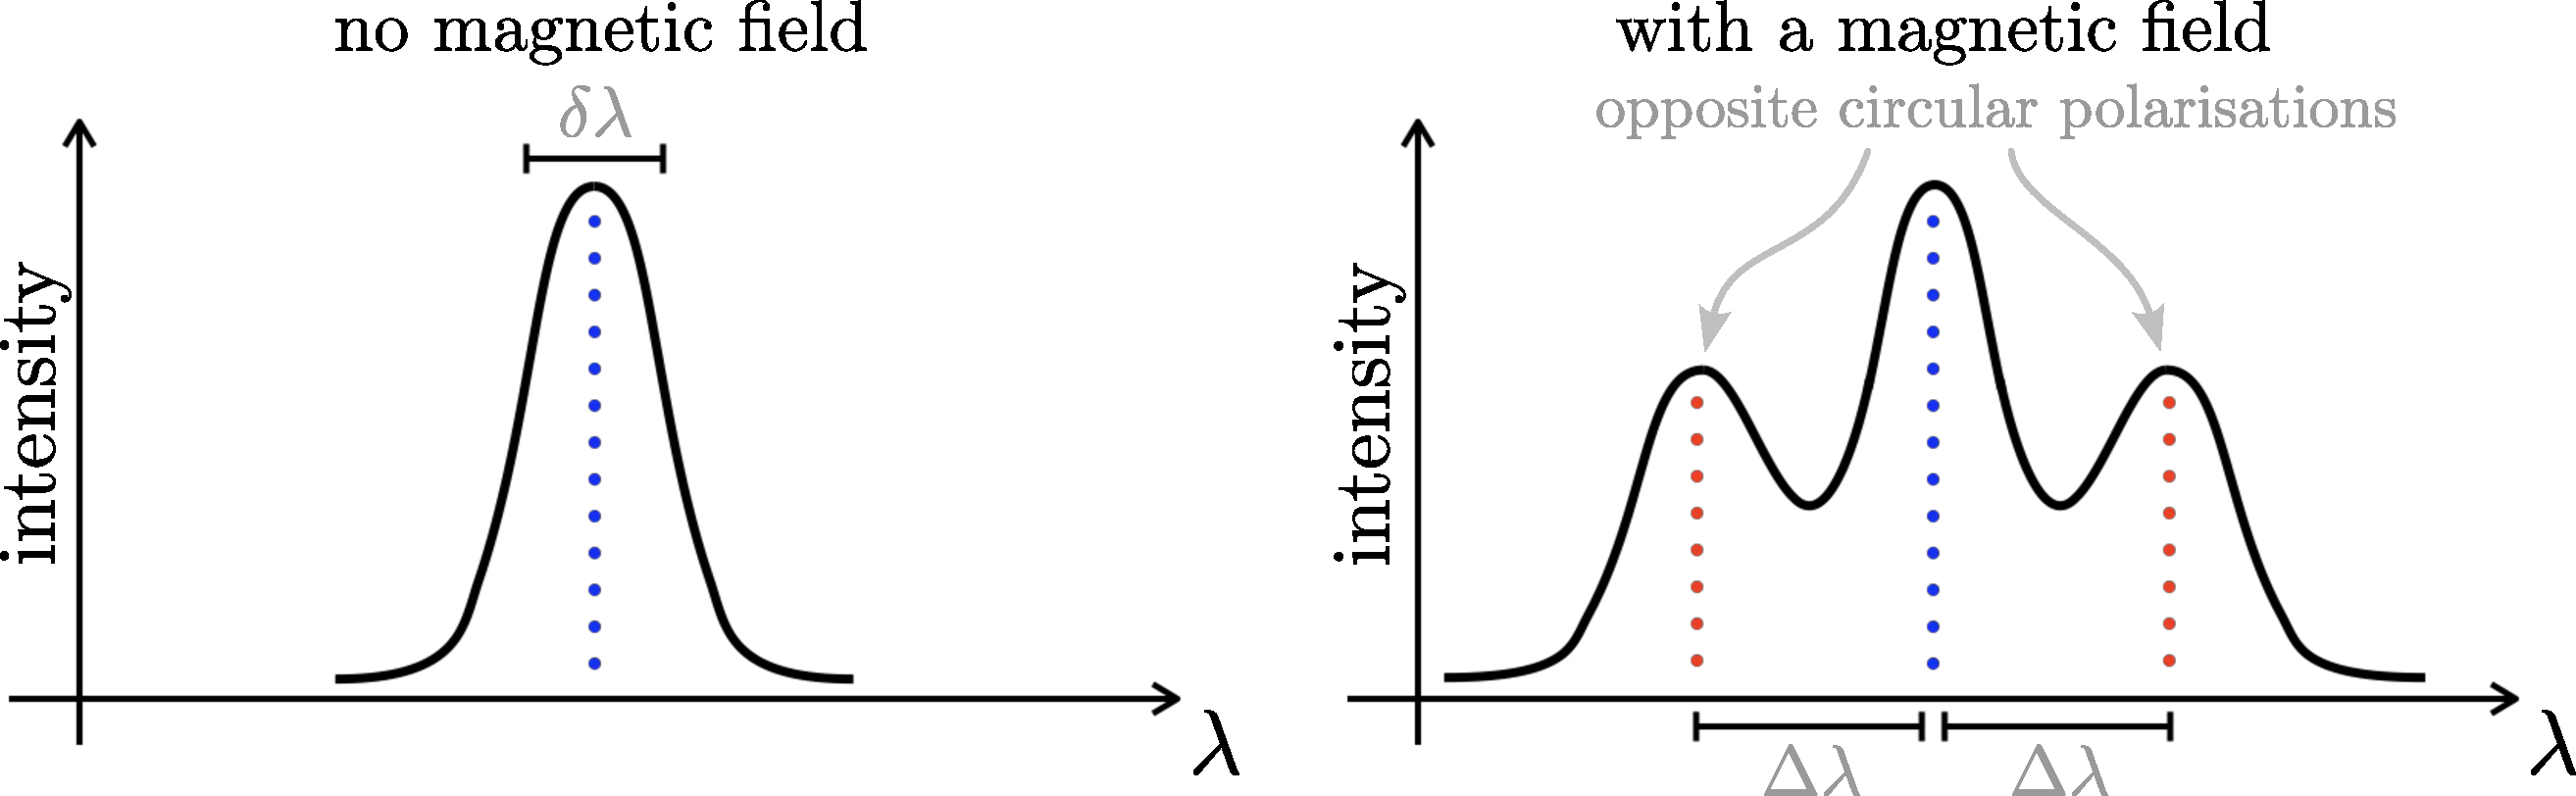
\includegraphics[width=\linewidth]{figures/introduction/zeeman.pdf}
    \caption{Schematic of Zeeman splitting in a spectral line. Without a magnetic field (left), a transition produces a single line with characteristic width $\delta\lambda$ set by thermal and turbulent Doppler broadening. In the presence of a magnetic field (right), the line splits into components with different circular polarisations that are shifted in frequency by $\Delta\lambda \propto b_\parallel$, where $b_\parallel$ is the line-of-sight component of the field. In this figure I have exaggerated the size of the shift for visiblity, but in practice in the interstellar medium, the shift $\Delta\lambda$ is almost always smaller than the intrinsic linewidth $\delta\lambda$, and thus the shift is detected by detecting a residual after differencing the two polarisation components.}
    \label{fig:zeeman}
\end{figure}

This effect arises as a consequence of electrons carrying magnetic moments associated with their spin and orbital motion. In the absence of an external magnetic field, these moments have no preferred orientation, so the magnetic sublevels relevant to a given transition are degenerate, and the transitions only produce spectral lines at a single frequency. \DIFdelbegin \DIFdel{When }\DIFdelend \DIFaddbegin \DIFadd{However, when }\DIFaddend an external magnetic field is present, \DIFdelbegin \DIFdel{however, }\DIFdelend the field couples to the magnetic moments of bound electrons in the emitting or absorbing species, and exerts a torque that causes them to precess about the field\DIFdelbegin \DIFdel{direction}\DIFdelend \DIFaddbegin \DIFadd{'s orientation}\DIFaddend . In these configurations, the field favours orientations that are more closely aligned or anti-aligned, which lifts the degeneracy and shifts the corresponding transition's energy levels by a small amount. In turn, these energy shifts translate into small frequency offsets,
\begin{align}
    \Delta \lambda
        \propto b_\parallel
    ,
\end{align}
in the emitted or absorbed radiation.

Despite its apparent simplicity, Zeeman splitting is not trivial to apply in astronomy \citep[see details by \eg][]{brauer2017magnetic}. This is because the magnitude of the splitting, $\Delta \lambda$, depends on the transition's Zeeman coefficient (set by its effective Land\'e factor), so only a small set of species provide sufficiently large Zeeman sensitivity. In the interstellar medium, where magnetic fields are typically quite weak (at least compared to the plasma environments we can create in laboratories on Earth), this limits us to tracers like the atomic hydrogen 21-cm transition and molecules with large electronic magnetic moments, like OH, CN, CH, CCS, SO, and O$_2$. However, even for these tracers, $\Delta \lambda$ is usually much smaller than the observed line width $\delta \lambda$ set by thermal (and turbulent) Doppler broadening, so the Zeeman components are rarely resolved as separate peaks.

In practice, one therefore measures the associated circular-polarisation signature across the line profile. The split Zeeman components carry opposite circular polarisations, so splitting the signal into left- and right-circular polarisations and differencing them yields a characteristic antisymmetric residual whose amplitude is proportional to $b_\parallel$. Because many instrumental and sky-noise contributions enter both polarisation channels in a similar way, differencing suppresses the shared noise-modes and allows detection of much weaker splitting than would be possible from total intensity alone. Where it can be applied, Zeeman splitting provides a uniquely direct constraint on $b_\parallel$, which can be used to calibrate and validate field estimates inferred from synchrotron emission and Faraday rotation.

\subsubsection{Synchrotron Radiation}
\label{sec:how-we-see:synchrotron}

At radio wavelengths, synchrotron radiation from relativistic electrons provides one of the most widely used tracers of cosmic magnetism \citep{vallee2011magnetic}. As these electrons propagate through magnetised environments, their trajectories are bent by magnetic tugs (the Lorentz force) into gyrating trajectories about magnetic field lines. Since these particles experience a constant acceleration, they radiate, and since they are relativistic, their radiation is strongly beamed along the instantaneous direction of motion. An ensemble of gyrating electrons then produces diffuse radiation whose intensity depends on the magnetic field strength, $b$, and on the energy distribution of the radiating electrons, while its polarisation traces the geometry of the plane-of-sky component, $b_\perp$. \autoref{fig:synchrotron} illustrates the basic geometry of this process.

\begin{figure}
    \centering
    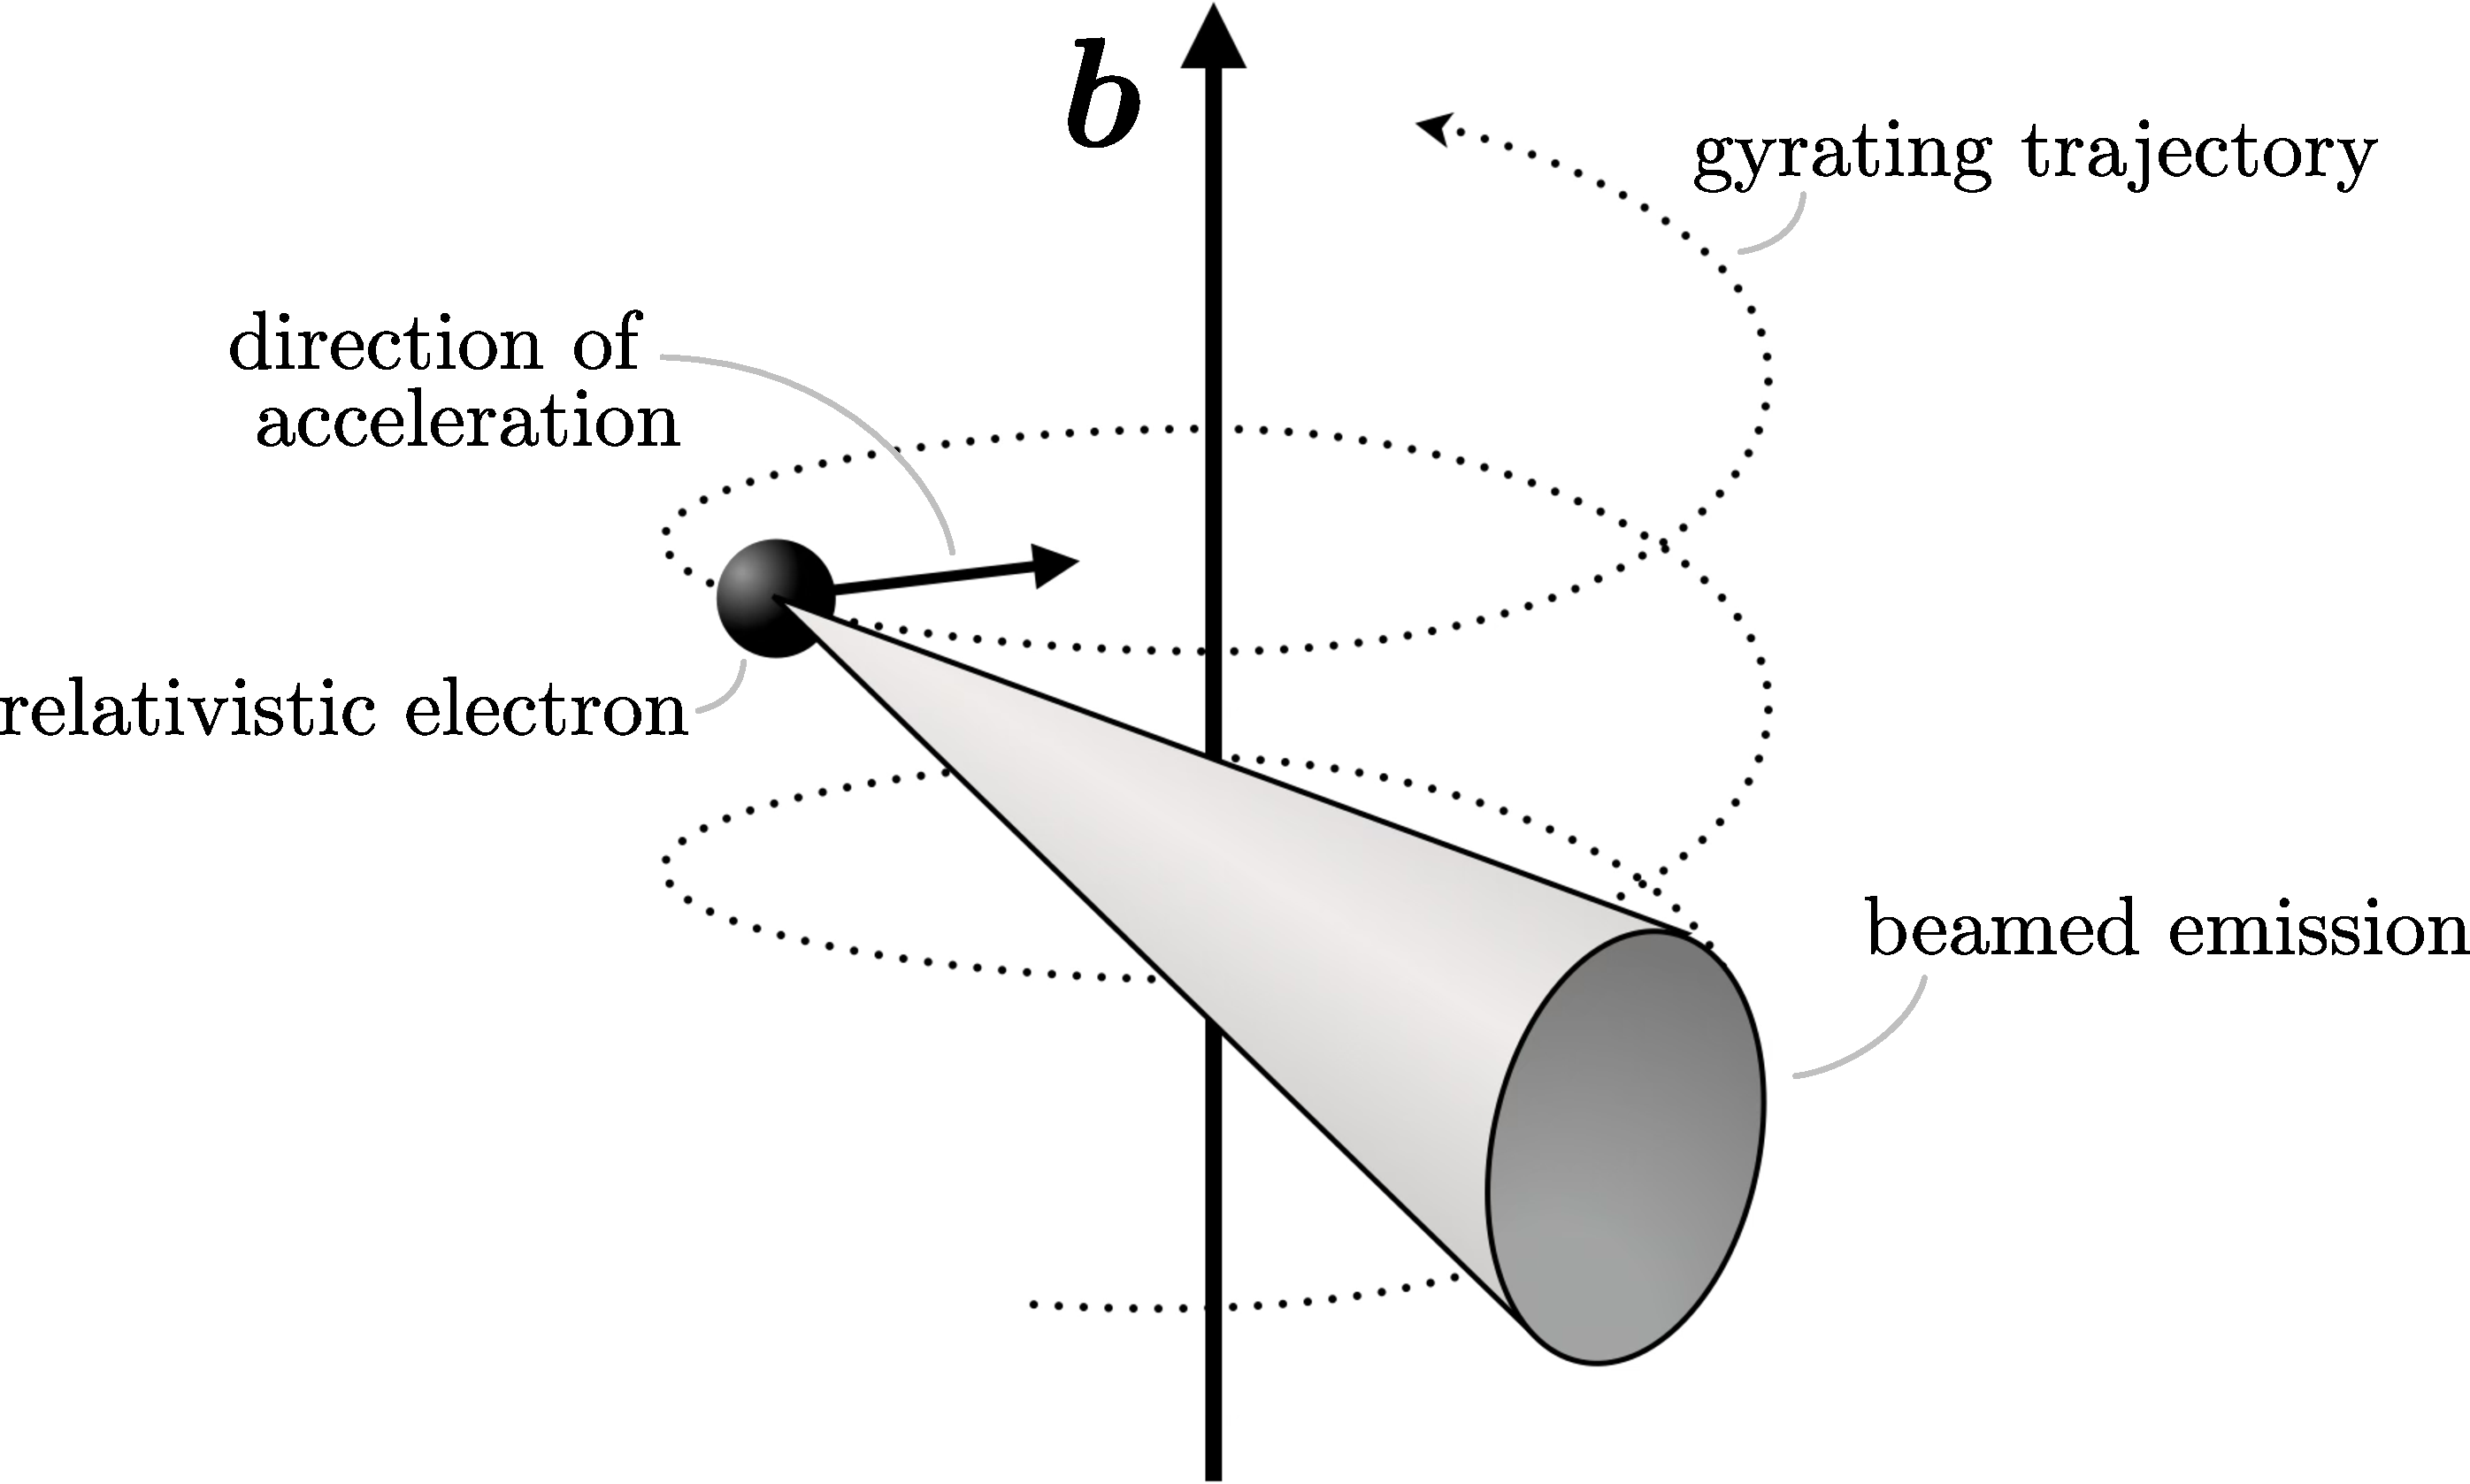
\includegraphics[width=0.85\linewidth]{figures/introduction/synchrotron.pdf}
    \caption{Schematic of synchrotron emission, adapted from \citet{shukurov2021astrophysical}. A relativistic electron gyrates about a magnetic field, $\mVector{b}$, with the Lorentz force providing an acceleration directed toward the local centre of its trajectory. Because the electron is relativistic, the emitted radiation is strongly beamed along the instantaneous direction of motion, producing a narrow emission cone.}
    \label{fig:synchrotron}
\end{figure}

At longer radio wavelengths ($\lambda \sim \mathrm{cm}-\mathrm{m}$), synchrotron emissivity depends on the relativistic electron population and the magnetic field strength,
\begin{align}
    \epsilon_\lambda
        \propto n_\mathrm{re}\, b^{(p+1)/2}\, \lambda^{(p-1)/2}
    ,
\end{align}
for an electron energy distribution $\mdd n / \mdd E_e \propto E_e^{-p}$, where $n_\mathrm{re}$ is the relativistic electron number density, and $p$ is the electron spectral index. Synchrotron emission therefore constrains $b$ only in combination with $n_\mathrm{re}$. The intensity alone cannot be inverted to a magnetic field strength without a closure for $n_\mathrm{re}$ (or, more generally, for the cosmic-ray electron energy density). However, a common closure, and perhaps the simplest choice, is to assume an approximate equipartition between the energy densities of cosmic rays and magnetic fields \citep{beck2005revised}, which yields a practical estimate of $b$, but inherits uncertainty from assumptions about the particle spectrum, filling factors, and the degree to which local energy balance holds true \citep{seta2019revisiting}.

Synchrotron emission is intrinsically linearly polarised, and so polarisation angle provides a second observable probe, alongside the total intensity, revealing the orientation of the ordered component of $b_\perp$. That said, the measured angle is not, in general, the same as the emission angle, because propagation through a magnetised plasma can rotate the plane of polarisation (see Section~\ref{sec:how-we-see:faraday-rotation}). Moreover, the polarisation fraction is also often suppressed, since the observed signal could contain many emitting regions along the line-of-sight (and across the telescope beam), so polarisation contributions may partially cancel. Polarisation, therefore, tends to mainly diagnose the degree of ordering in $b_\perp$, but cannot by itself tell whether the ordered component reflects a truly coherent field, or an anisotropically aligned, turbulent one.

At higher energies, relativistic electrons can also produce X-ray emission through inverse Compton scattering, which in some environments provides a useful complement to synchrotron measurements. For example, in radio-galaxy lobes (where seed photons are dominated by the cosmic microwave background) and in compact hotspots (where synchrotron self-Compton emission can apply), magnetic field strengths can be constrained from the ratio of synchrotron to inverse-Compton flux \citep[see reviews by \eg][]{worrall2002gaseous, hardcastle2020radio}.

\subsubsection{Faraday Rotation}
\label{sec:how-we-see:faraday-rotation}

Faraday rotation probes magnetic fields through their effect on the propagation of linearly polarised radiation, and explains why the polarisation angle (the orientation of the projected electric-field vector) inferred from synchrotron emission may be different from its emitted angle \citep{brentjens2005faraday}. This is because, as polarised radiation propagates through an ionised medium, the linear polarisation plane rotates by an amount proportional to $\lambda^2$, where $\lambda$ is the wavelength of the light (this is illustrated in \autoref{fig:faraday}). The rate of this rotation is quantified by the rotation measure,
\begin{align}
    \mathrm{RM}
        \propto \int n_\mathrm{th}\, b_\parallel \, \mdd l
    , \label{eqn:how-we-see:RM}
\end{align}
where $n_\mathrm{th}$ is the thermal (free) electron number density, and $b_\parallel$ is the line-of-sight component of the magnetic field \citep{haverkorn2014magnetic}. Faraday rotation therefore constrains $b_\parallel$ through the magnitude and sign of $\mathrm{RM}$, but only in combination with an understanding for the thermal electron distribution, since the integral in \autoref{eqn:how-we-see:RM} is weighted by $n_\mathrm{th}$ and by the path length through the plasma.

\begin{figure}
    \centering
    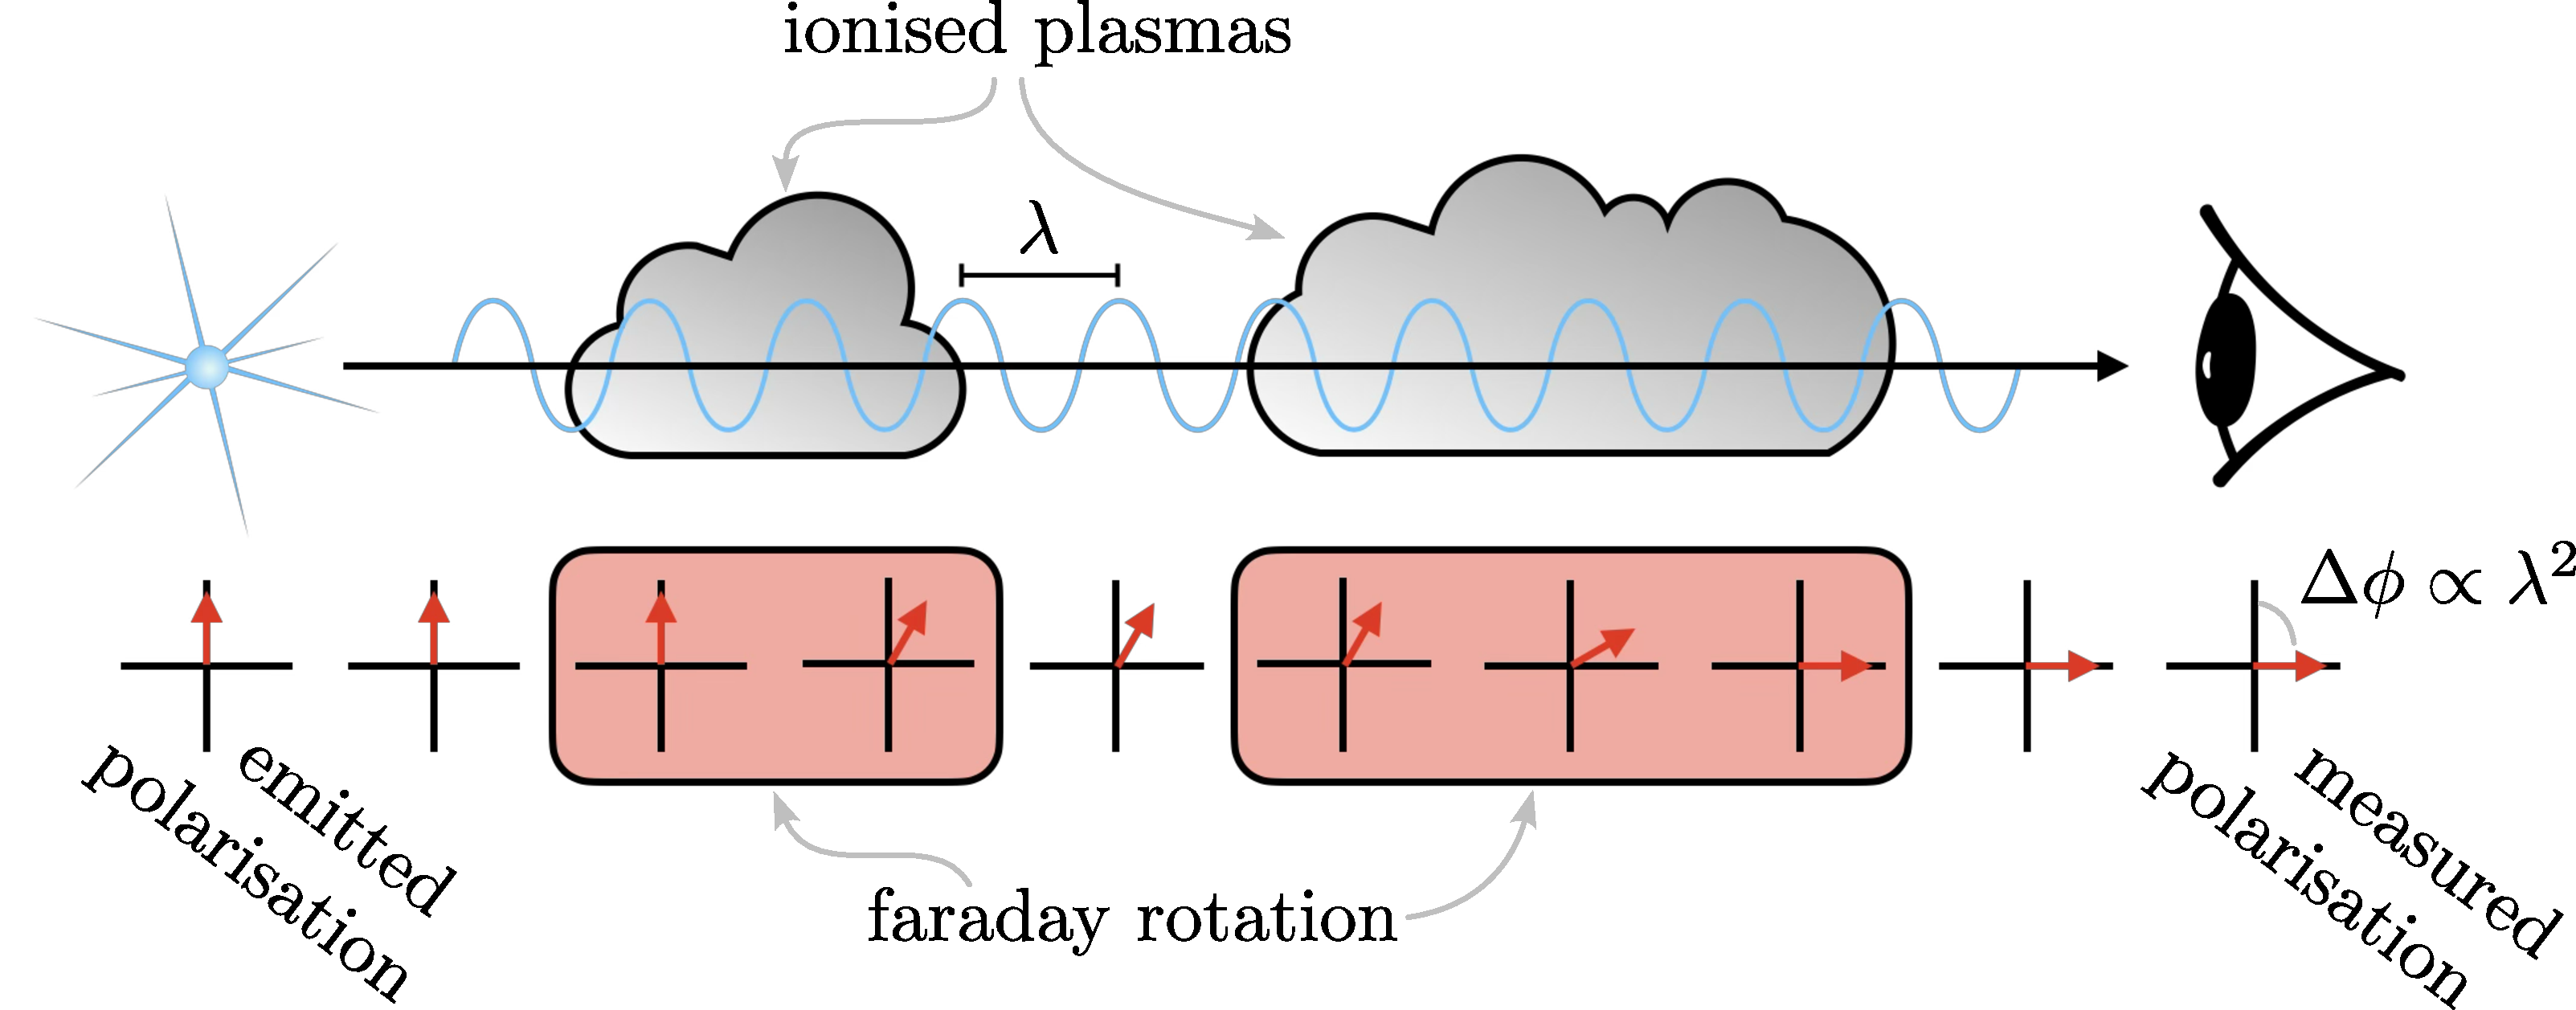
\includegraphics[width=\linewidth]{figures/introduction/faraday.pdf}
    \caption{Schematic of Faraday rotation. Linearly polarised radiation emitted by a background source propagates through regions of ionised plasma, causing the polarisation angle, $\phi$, to rotate. The accumulated rotation depends on wavelength as $\Delta\phi \propto \lambda^{2}$, with the rate of rotation quantified by the rotation measure (see \autoref{eqn:how-we-see:RM}).}
    \label{fig:faraday}
\end{figure}

In realistic astrophysical plasmas, however, $b_\parallel$ can reverse many times along the line of sight, so positive and negative contributions often lead to integrated $\mathrm{RM}$ that nearly cancel \citep{haverkorn2014magnetic}. As a consequence, in practice, $\mathrm{RM}$ primarily traces the net, large-scale component of $b_\parallel$, while small-scale structures are imprinted as fluctuations in $\mathrm{RM}$ across neighbouring sightlines, and as depolarisation of the polarised emission. Interpreting $\mathrm{RM}$ in terms of a field strength \DIFdelbegin \DIFdel{, }\DIFdelend therefore benefits from independent constraints on $n_\mathrm{th}$, and from combining Faraday rotation with synchrotron intensity and polarisation to jointly constrain $b_\parallel$ and $b_\perp$.

\subsubsection{Dust Polarisation}
\label{sec:how-we-see:polarisation}

\begin{figure}
    \centering
    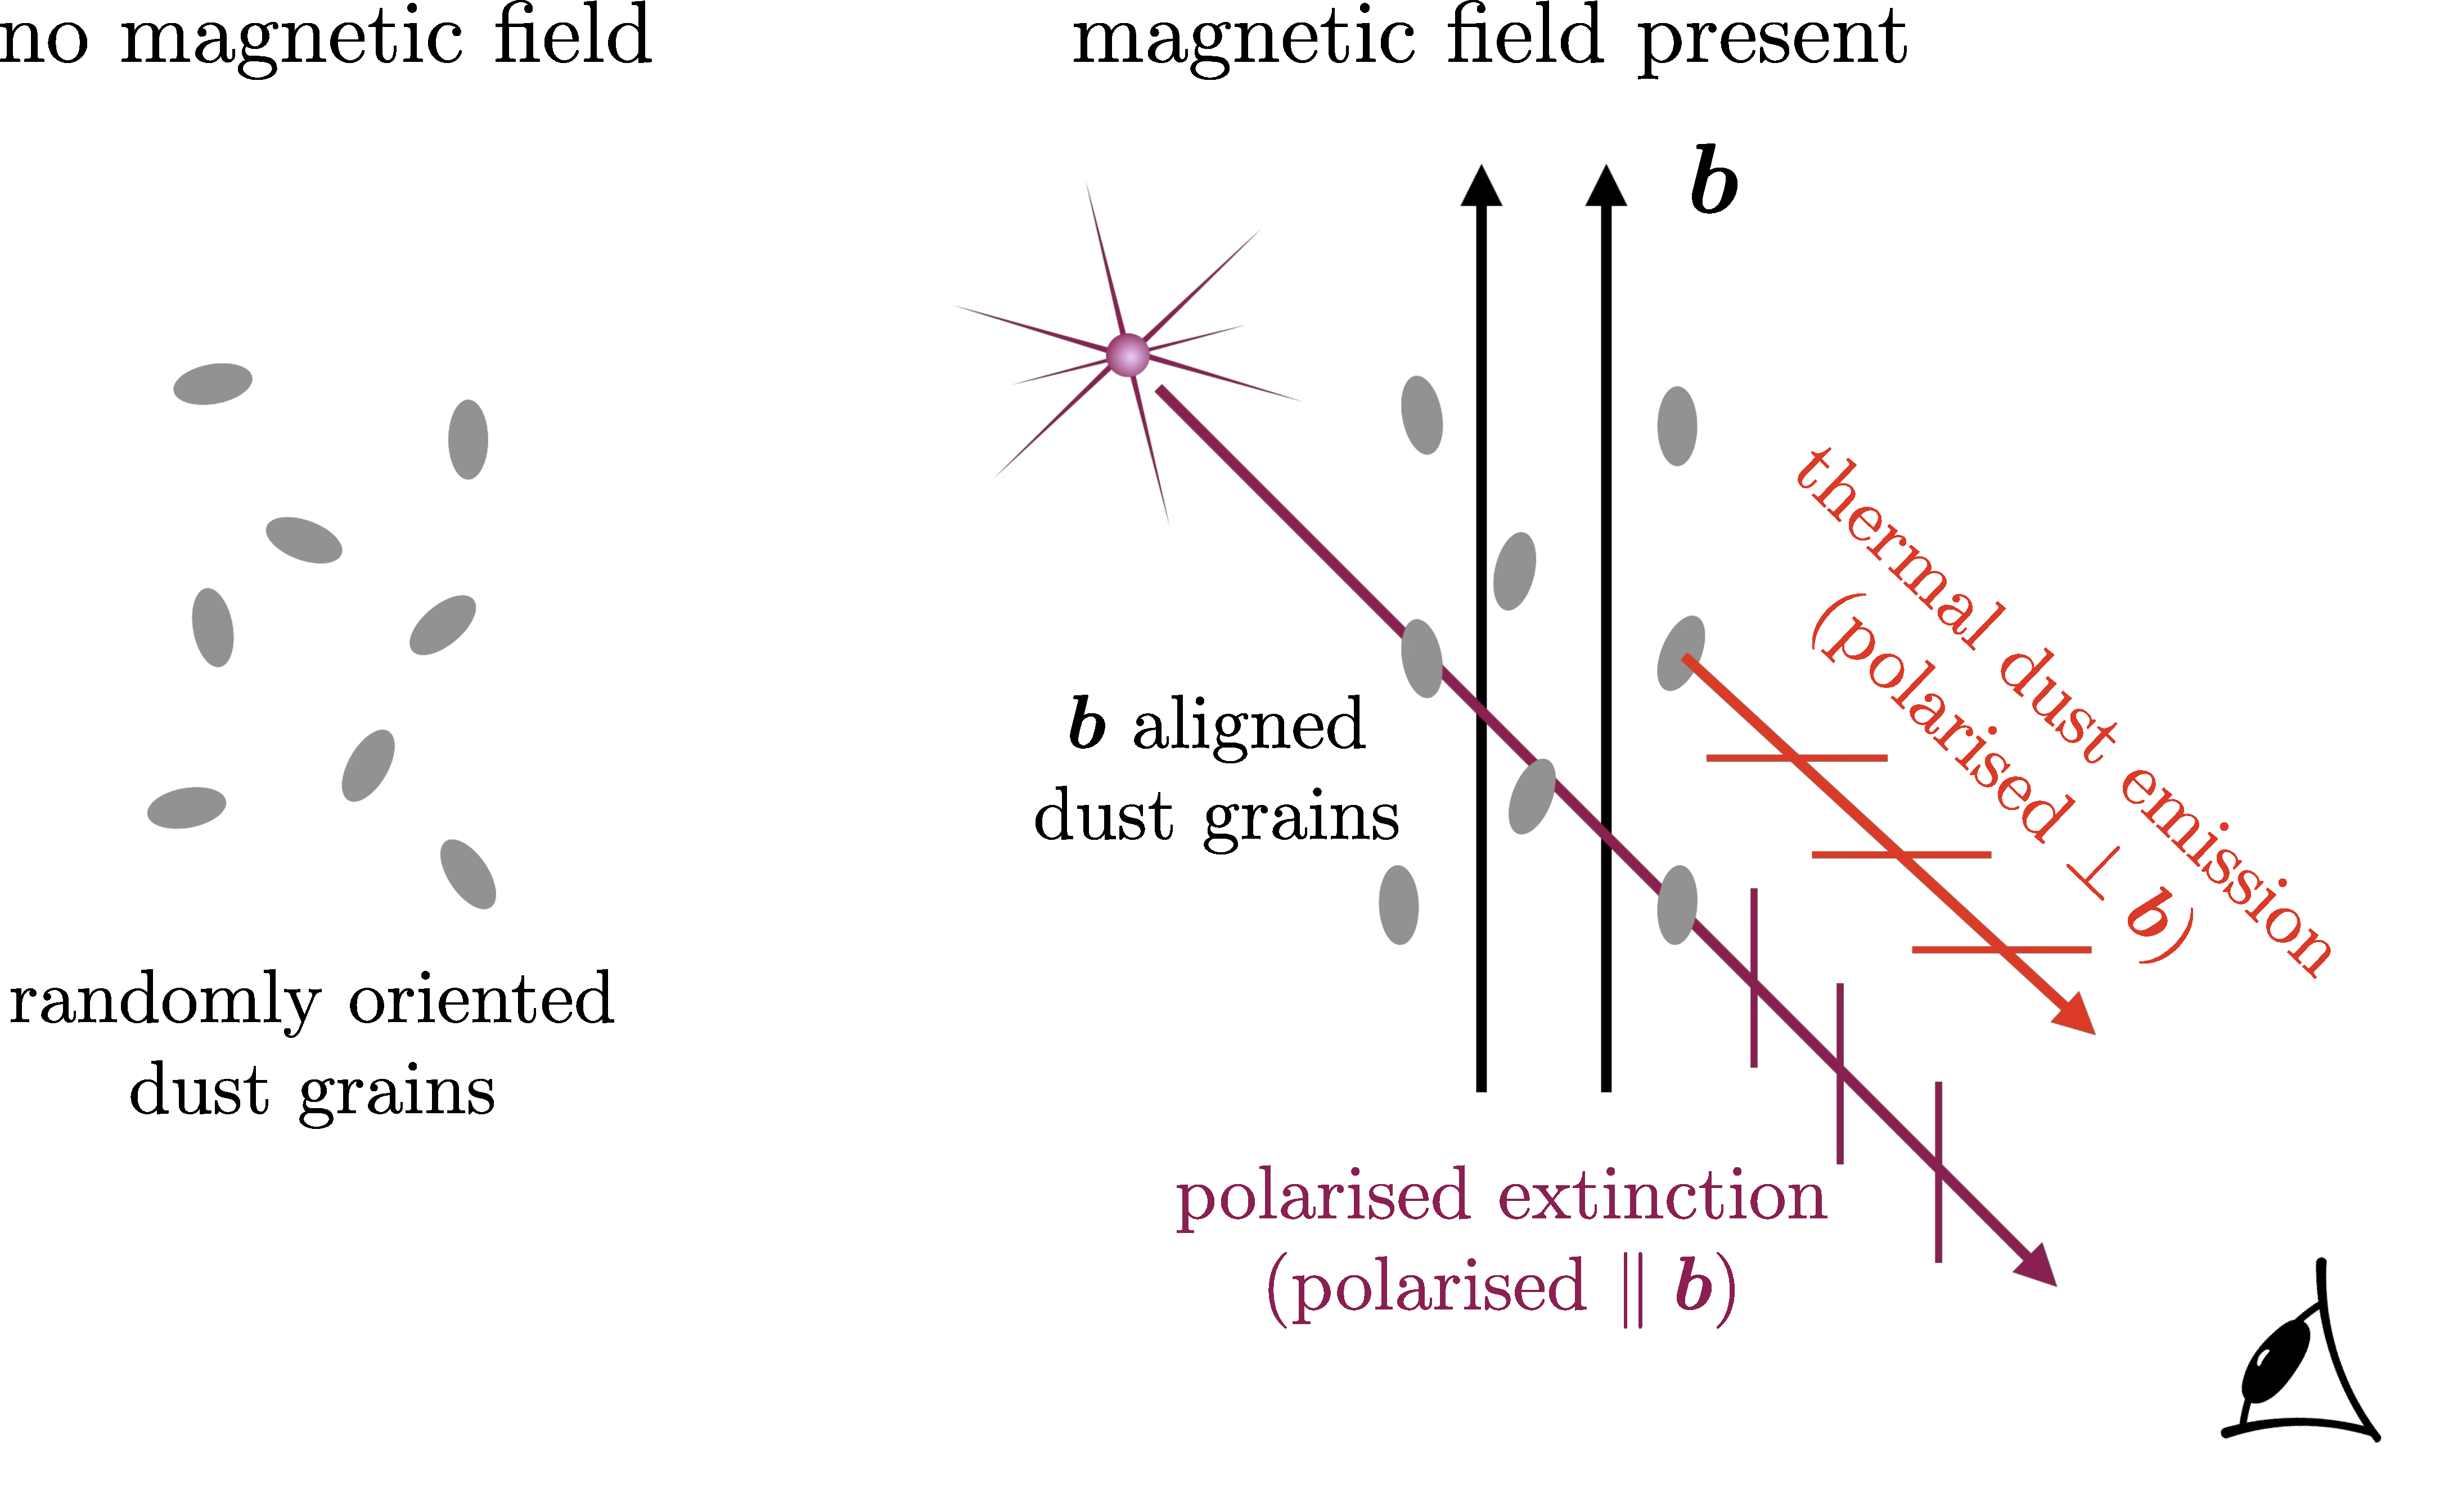
\includegraphics[width=\linewidth]{figures/introduction/dust.pdf}
    \caption{Schematic of dust polarisation, adapted from a lecture by Jennifer Schober. In the absence of a magnetic field (left), dust grains are randomly oriented and produce little net linear polarisation. When a magnetic field is present (right), elongated grains become preferentially aligned with the local field direction, $\mVector{b}$, so that both polarised extinction of background starlight (with polarisation aligned parallel to $\mVector{b}$) and polarised thermal emission (with polarisation aligned perpendicular to $\mVector{b}$) can be used to trace magnetic-field orientation.}
    \label{fig:dust}
\end{figure}

The final probe we will discuss is dust polarisation, which, like synchrotron polarimetry, traces the plane-of-sky magnetic field component, $b_\perp$, through measurements of linear polarisation. At far-infrared and sub-millimeter wavelengths\footnote{
    Faraday rotation is typically negligible at these wavelengths. To see why, consider \autoref{eqn:how-we-see:RM} for a typical diffuse ISM sightline, where $n_\mathrm{th}\sim 0.03~\mathrm{cm^{-3}}$, $b_\parallel\sim 3~\mu\mathrm{G}$, and $L\sim 1~\mathrm{kpc}$. With this, an order-of-magnitude analysis gives $\mathrm{RM}\sim 10^2~\mathrm{rad\,m^{-2}}$. Since the amount of rotation scales as $\lambda^2$, an order-unity rotation requires $\lambda \gtrsim 10^{-1}~\mathrm{m}$, and therefore, at wavelengths associated with dust polarisation, namely $\lambda \lesssim 10^{-3}~\mathrm{m}$, rotation is suppressed; for the same sightline, the rotation at $\lambda\lesssim 10^{-3}~\mathrm{m}$ is smaller than at $\lambda\sim 10^{-1}~\mathrm{m}$ by a factor $\left(10^{-3}/10^{-1}\right)^2 \sim 10^{-4}$, so dust polarisation can usually be interpreted without an $\mathrm{RM}$ correction.
    \label{fnote:faraday}
}, these polarisation measurements are dominated by thermal emission from interstellar dust grains, whereas, at optical and near-infrared wavelengths, they are dominated by the polarised extinction of background starlight by dust. In both regimes, a preferred polarisation emerges because interstellar grains are charged and typically elongated rather than spherically symmetric, which leads to them becoming preferentially aligned with the local magnetic field \citep{andersson2015interstellar}. This alignment makes their absorption and emission anisotropic, producing linearly polarised radiation whose orientation traces the ordered component of $b_\perp$ in the dust-bearing gas (see \autoref{fig:dust}).

Because dust is abundant in the cold and warm phases of the interstellar medium, particularly in filaments and star-forming clouds, dust polarisation is often the most effective cartographer of $b_\perp$ in these environments \citep{collaboration2015planck}. However, dust polarisation on its own only provides a very limited direct constraint on field strength, since the polarisation fraction does not only depend on the field geometry, but also on dust grain properties, alignment efficiency, and line-of-sight averaging. Its primary utility is therefore in constraining the orientation and coherence of $b_\perp$ in dense, dusty environments where synchrotron emission may be weak and Faraday rotation may be hard to interpret.

The \textit{structure} of polarisation maps can nevertheless be used to obtain an estimate of $b_\perp$, where a popular approach is the Davis-Chandrasekhar-Fermi method \citep{davis1951polarization, chandrasekhar1953magnetic}, in which turbulent motions are assumed to perturb the plane-of-sky field, producing a dispersion in polarisation angles, $\sigma_\phi$, whose magnitude reflects the ratio of turbulent to magnetic restoring stresses. Combining $\sigma_\phi$ with an estimate of the gas mass density, $\rho$, and a one-dimensional velocity dispersion, $\sigma_u$, inferred from line widths yields an order-of-magnitude estimate,
\begin{align}
    b_\perp
        \sim Q \, \sqrt{4\pi\rho} \, \frac{\sigma_u}{\sigma_\phi}
    ,
\end{align}
where $Q$ is an order-unity calibration factor that absorbs geometric and line-of-sight effects \citep[\eg][]{ostriker2001density}.

\subsection{A (Brief) Excursion Through Astrophysical Plasmas}
\label{sec:what-we-see}

Zeeman splitting has been successfully applied to star-forming, dense molecular clouds, where measurements indicate $b \sim 10-100 \,\mu\mathrm{G}$ in regions undergoing active collapse and feedback (\eg \citealt{sarma2013very}; see also, \eg \citealt{pattle2022magnetic} for a thorough review). Independent dust polarisation and Faraday-based observations are consistent with these estimates, and indicate that the orientation of $b$ remains ordered over entire \DIFdelbegin \DIFdel{cloud complexes }\DIFdelend \DIFaddbegin \DIFadd{clouds, at least }\DIFaddend on scales of $\sim 10 \,\mathrm{pc}$ \citep{collaboration2015planck, fissel2016balloon, tahani2018helical}. Moreover, dust polarisation measurements at far-infrared wavelengths ($\lambda \sim 50-200 \,\mu\mathrm{m}$) extend this picture to denser regions of the Milky Way, revealing similarly ordered magnetic structures in dense, dust-obscured regions of active star formation \citep{lopez2020sofia}. \DIFdelbegin \DIFdel{While these }\DIFdelend \DIFaddbegin \DIFadd{These }\DIFaddend different probes and surveys point to a common conclusion for magnetic fields in the Milky Way's dense ISM and star-forming clouds: magnetic energy densities fluctuate about equipartition with kinetic and gravitational energy densities\DIFaddbegin \DIFadd{. However}\DIFaddend , one needs to be careful interpreting these measurements directly\DIFdelbegin \DIFdel{. Numerical }\DIFdelend \DIFaddbegin \DIFadd{, since numerical }\DIFaddend simulations have shown that projection effects and intermittency can complicate the mapping between observed and intrinsic field properties \citep{camacho2023kinetic, hu2023sub, seta2025magnetic}.

Beyond the Milky Way, nearby spiral galaxies provide some of the clearest evidence for galactic magnetic fields. In the grand-design spiral galaxy M51, for example, synchrotron polarisation and rotation measure observations at $6 \,\mathrm{cm}$ reveal a magnetic field organised on $\sim \mathrm{kpc}$ scales, closely tracing the spiral arms of the disc \citep{fletcher2011magnetic}. In contrast, dust polarisation measurements at $154 \,\mu\mathrm{m}$ reveal a field that varies on $\sim 10 \,\mathrm{pc}$ scales across regions of dense molecular ISM \citep{borlaff2021extragalactic}. These measurements (see \autoref{fig:m51}) probe different phases of the ISM, with dust polarisation tracing cold, dense gas that is sensitive to the plane-of-sky orientation of $b$, while synchrotron emission and Faraday rotation sample diffuse magnetised plasma distributed across the disc. The coexistence of these signatures suggests that the galactic magnetic field carries a large-scale component organised across the disc, alongside a component that varies across the turbulent, star-forming ISM. Similar dust polarisation observations with ALMA show that this is not unique to M51, and is instead a common feature of present-day spiral galaxies \citep[\eg][]{belfiori2025dust, de2025grand}.

\begin{figure}
    \centering
    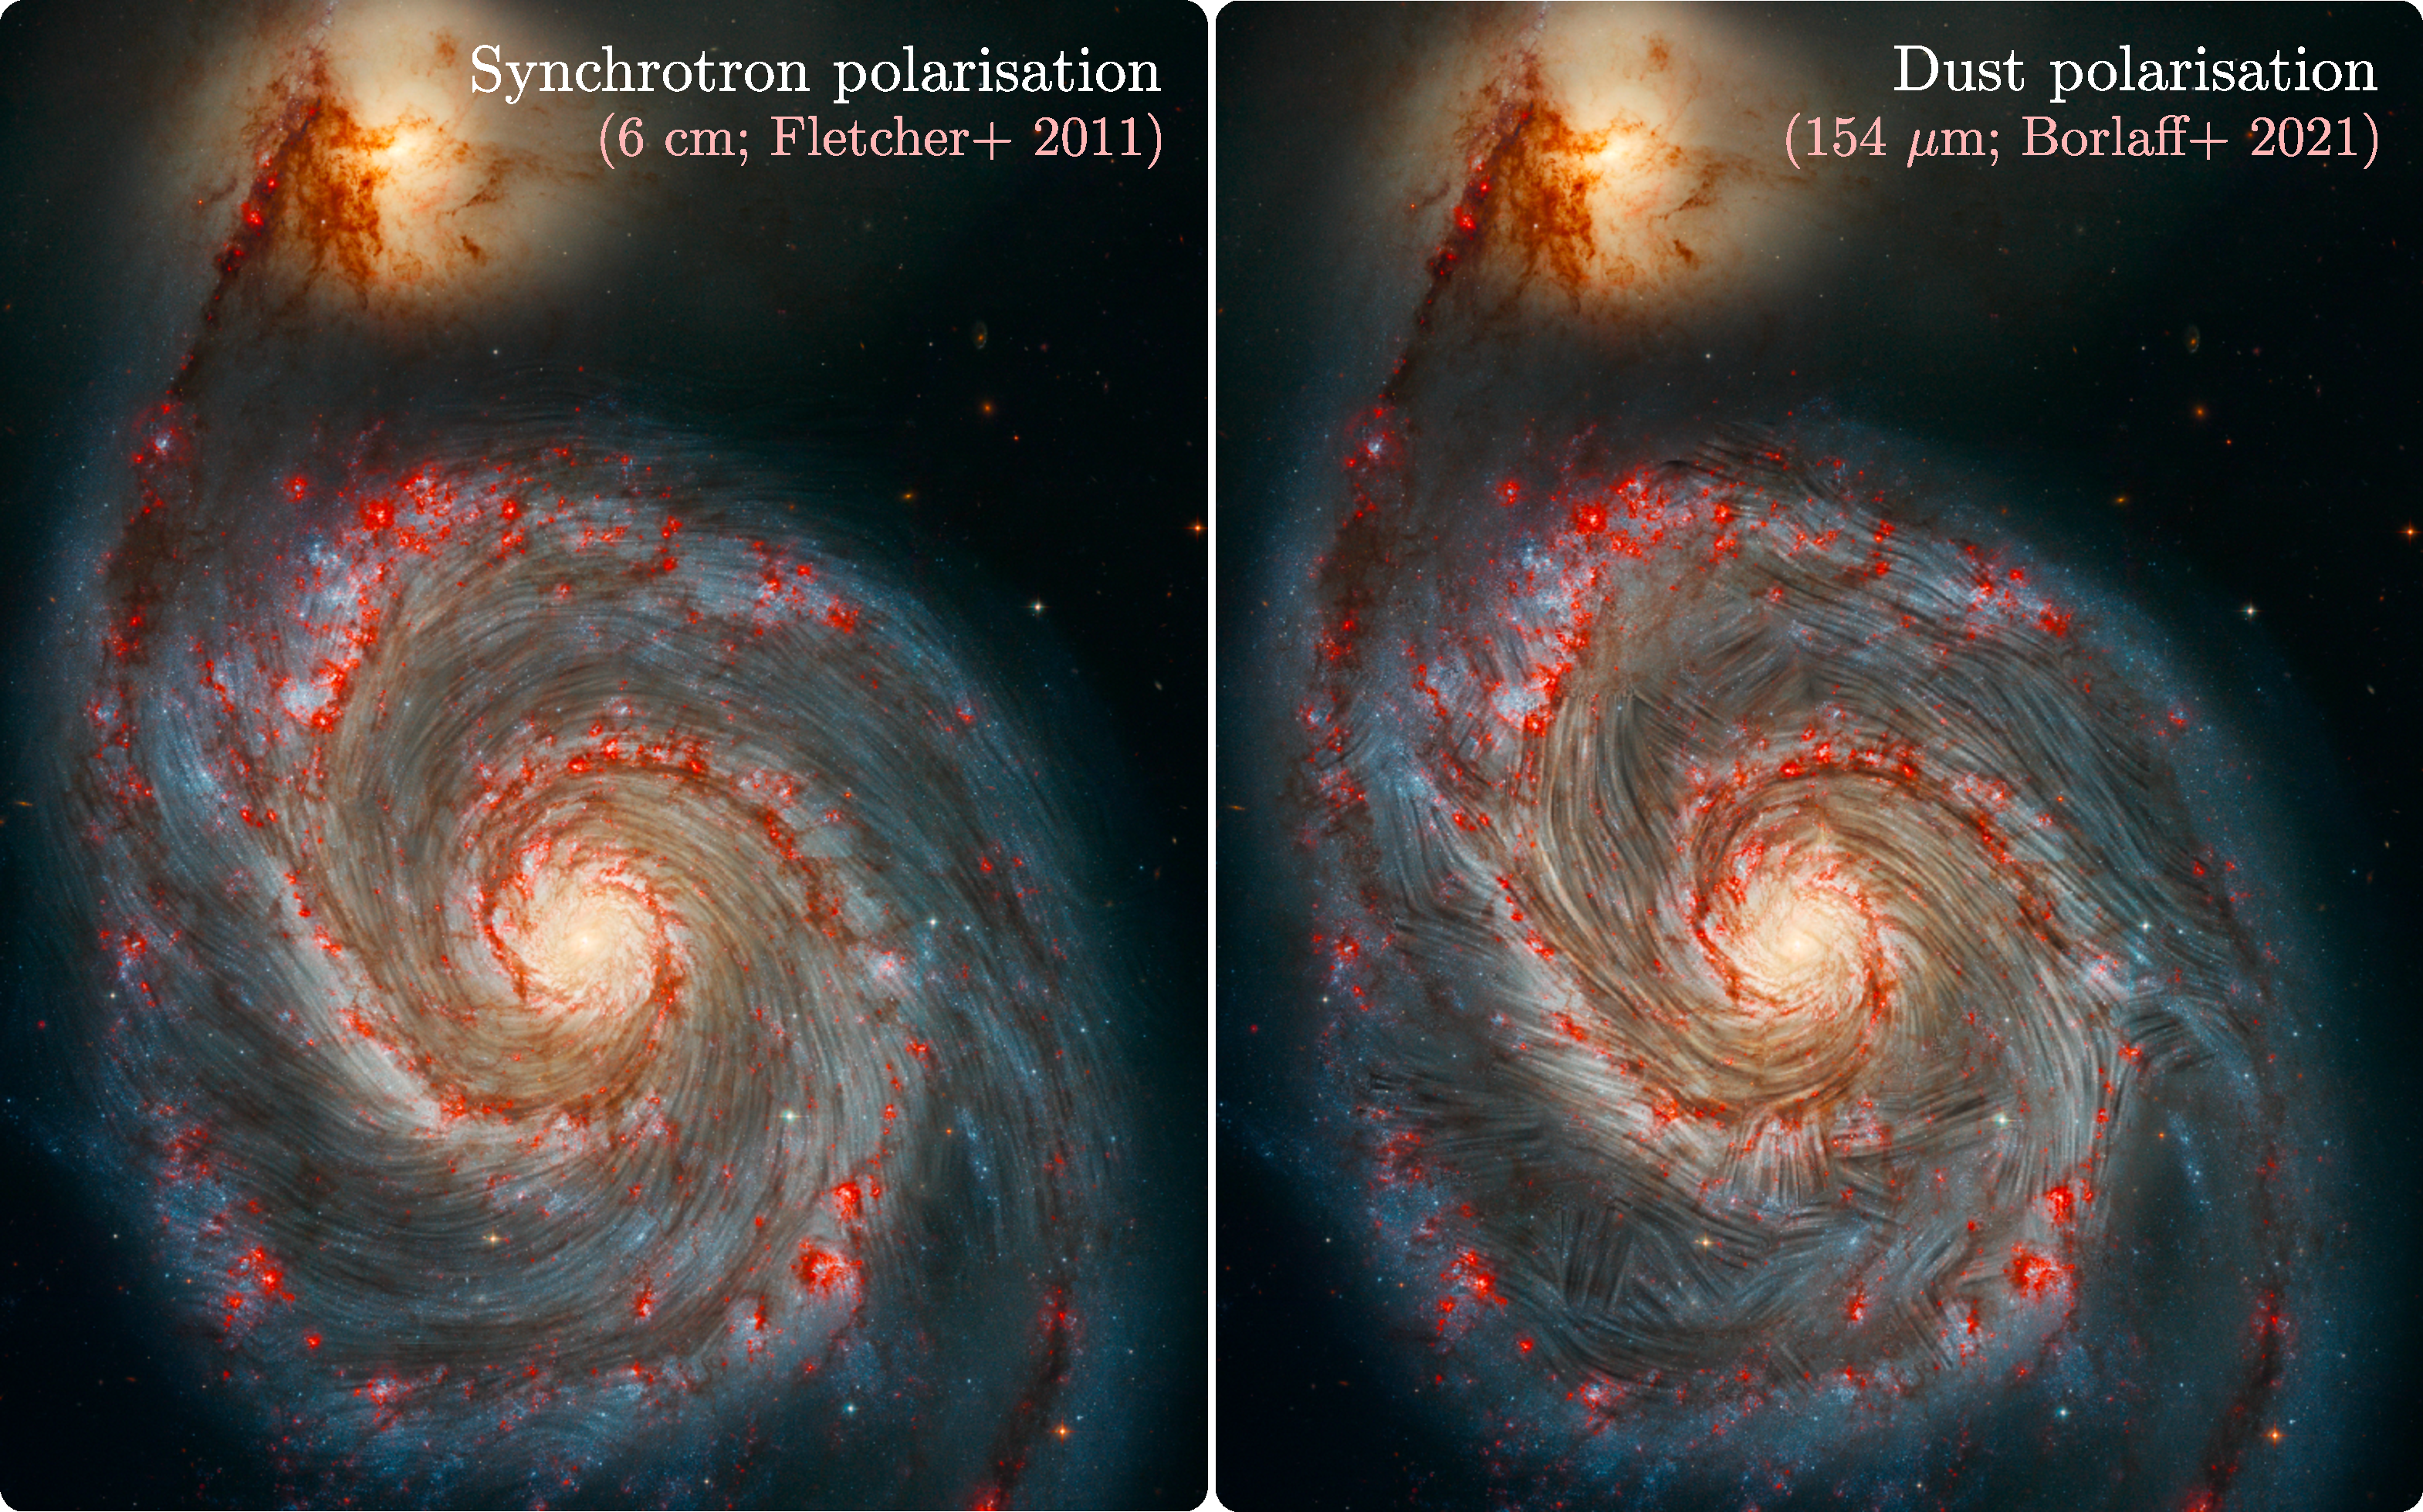
\includegraphics[width=\linewidth]{figures/introduction/M51.pdf}
    \caption{Plane-of-sky magnetic-field orientation in M51 inferred from polarised emission tracing different phases of the interstellar medium. In the left panel, synchrotron polarisation measured at $6\,\mathrm{cm}$ probes the ordered component of the plane-of-sky field, $b_\perp$, in diffuse magnetised plasma \citep{fletcher2011magnetic}; in the right panel, dust polarisation at $154\,\mu\mathrm{m}$ samples colder, denser gas \citep{borlaff2021extragalactic}. In both cases, the polarisation angle constrains the orientation of $b_\perp$ (with only the synchrotron angle susceptible to Faraday rotation along the line of sight; see \autoref{fnote:faraday}).}
    \label{fig:m51}
\end{figure}

Perhaps the most surprising observational result, which\DIFaddbegin \DIFadd{, }\DIFaddend as we discuss below, sits at odds with the current picture of magnetogenesis, is that coherent magnetic fields already appear to be present on $\sim\mathrm{kpc}$ scales in ``young'' galaxies. Rotation-measure studies at $z \sim 1$ indicate ordered line-of-sight field components comparable to those in nearby systems \citep{bernet2008strong, sur2018faraday}. More recently, ALMA detections of polarised dust emission have extended this picture to earlier epochs, revealing ordered plane-of-sky magnetic structures at $z \approx 2.6$ and $z \approx 5.6$ on scales of several $\mathrm{kpc}$ \citep{geach2023polarized, chen2024kiloparsec}. This is particularly surprising, because these ordered fields are usually associated with mechanisms that rely on sustained coherent rotation to organise magnetic structure on galactic scales. These galaxies, however, are placed at epochs where rotationally supported discs are generally not expected to have fully formed (\citealt{geach2023polarized} estimate a dynamo number $\mathcal{D} \approx 3$; see \S\ref{sec:evolve:lsd}). The presence of coherent magnetic fields at such early times therefore poses a significant challenge, and motivates a closer exploration of the circumstances and conditions under which large-scale magnetic structures could be generated in young systems.


\section{Modelling Magnetised Flows}
\label{sec:modelling}

In this chapter we introduce the theoretical framework used to describe the dynamics of magnetised astrophysical flows. Our starting point is a macroscopic fluid description, which is appropriate on the length and timescales relevant for galaxy evolution, where the collective behaviour of large numbers of particles dominates over individual kinetic effects. Since these particles are charged, this naturally leads to the magnetohydrodynamic (MHD) framework, which couples fluid dynamics to electromagnetic fields and provides a self-consistent description of conducting plasmas; these equations form the foundation for the remainder of this thesis.

We begin by introducing the fluid framework and its governing conservation laws (\S\ref{sec:modelling:fluid}), before extending this description to magnetised matter in the MHD framework (\S\ref{sec:modelling:mhd}). We then discuss how magnetic fields can be generated from initially unmagnetised conditions (\S\ref{sec:modelling:magnetogenesis}), and conclude by outlining the principal modes through which magnetic fields subsequently evolve and are maintained in astrophysical systems (\S\ref{sec:evolve}).

\subsection{The Fluid Framework}
\label{sec:modelling:fluid}

Our Universe is made up of many, many particles, each of which is governed, at its most fundamental level, by quantum physics. However, on the astrophysical scales relevant for galaxy dynamics, quantum wave effects are negligible, so particle motion can be described classically, with trajectories determined by Newton's laws of motion. On these scales, tracking trajectories for each particle quickly becomes impractical, since the number of particles in almost all astrophysical systems is enormous. It is instead more useful to adopt a statistical description of particle populations, whereby the collective properties of particles are described through a distribution function $\phi(\mVector{x}, \mVector{v}, t)$, which gives the number density of particles in phase space $(\mVector{x}, \mVector{v})$, where $\mVector{x}$ is the particle's real-space position, $\mVector{v}$ is its velocity, and $t$ is time. At fixed $\mVector{x}$ and $t$, integrating $\phi$ over all velocities gives the local number density,
\begin{align}
    n(\mVector{x}, t)
        \equiv \int \phi(\mVector{x}, \mVector{v}, t)  \mdd^3v .
\end{align}
From this, we can immediately define macroscopic fields describing the fluid of interest through velocity moments of $\phi$. In particular, the fluid density, fluid velocity, and specific (\ie per unit mass) total energy are defined as
\begin{align}
    \rho(\mVector{x}, t)
        &\equiv m \int \phi(\mVector{x}, \mVector{v}, t)  \mdd^3v
        , \\
    \mVector{u}(\mVector{x}, t)
        &\equiv \frac{m}{\rho(\mVector{x}, t)} \int \mVector{v} \phi(\mVector{x}, \mVector{v}, t)  \mdd^3v
        , \\
    \psi^{*}_\mathrm{tot}(\mVector{x}, t)
        &\equiv \frac{m}{2\rho(\mVector{x}, t)}\int \mVector{v}^{ 2} \phi(\mVector{x}, \mVector{v}, t)  \mdd^3v
        ,
\end{align}
with $m$ the particle mass. From this, we can also define other useful quantities, like the specific kinetic energy $\psi^{*}_\mathrm{kin} = u^2 / 2$, and the specific internal energy $\psi^{*}_\mathrm{int} = \psi^{*}_\mathrm{tot} - \psi^{*}_\mathrm{kin}$.

To obtain evolution equations for these macroscopic fields, we require an evolution equation for $\phi$ itself. An intuitive foundation is to realise that conservation of particles in phase space implies a continuity equation of the form
\begin{align}
    \mppFrac{\phi}{t}
        + \nabla_{\mVector{x}} \cdot \rbrac{\mVector{v} \phi}
        + \nabla_{\mVector{v}} \cdot \rbrac{\mppFrac{\mVector{v}}{t} \phi}
        = g(\phi)
        ,  \label{eqn:boltzmann}
\end{align}
where $\mdd_t \mVector{v}$ is the acceleration due to long-range (body) forces, and $g(\phi)$ is a nonlinear operator that captures the net effect of short-range interactions between particles, which, in neutral fluids, are limited to collisions. In collisionless flow regimes (often relevant for diffuse galactic halos and cosmic voids), $g(\phi) \approx 0$ (\autoref{eqn:boltzmann} reduces to the Vlasov equation), but in dense, collisional flow regimes (relevant for the dense interstellar medium and galactic discs), collisions are frequent and drive $\phi$ toward local equilibrium.

Now, notice that the macroscopic conservation laws do not require $g(\phi)$ to be \DIFdelbegin \DIFdel{explicitly stated }\DIFdelend \DIFaddbegin \DIFadd{stated explicitly}\DIFaddend . This is because taking velocity moments of \autoref{eqn:boltzmann} yields conservative evolution equations for mass, momentum, and energy, in which $g(\phi)$ drops out. Ultimately, this occurs because collisions conserve the number of particles, their momentum, and energy. To obtain a closed fluid system we need to relate the higher moments to the evolved fields through a closure; in the ideal-fluid (Euler) limit (where explicit heating and cooling terms are negligible) this enters through an equation of state $p(\rho, \psi^{*}_\mathrm{int})$, which leads to the evolution equations
\begin{align}
    \mppFrac{\rho}{t}
        + \nabla \cdot (\rho \mVector{u})
        &= 0
        , & \mbox{(mass)} \label{eqn:fluid:mass} \\
    \mppFrac{(\rho \mVector{u})}{t}
        + \nabla \cdot \rbrac{
            \rho (\mVector{u}\otimes\mVector{u})
            + p \mTensor{I}
            - \mTensor{V}
        }
        &= \rho \mVector{f}
        , & \mbox{(momentum)} \label{eqn:fluid:momentum} \\
    \mppFrac{(\rho \psi^{*}_\mathrm{tot})}{t}
        + \nabla \cdot \rbrac{
            (\rho \psi^{*}_\mathrm{tot} + p) \mVector{u}
            - \mTensor{V} \cdot \mVector{u}
        }
        &= \rho (\mVector{f}\cdot\mVector{u})
        , & \mbox{(total energy)} \label{eqn:fluid:energy}
\end{align}
that describe the conservative evolution of a single-species, electrically neutral fluid under body forces. Here $\mTensor{V}$ is the viscous stress tensor, which captures the anisotropic part of the pressure (momentum-flux) tensor beyond the Euler closure (isotropic pressure\DIFdelbegin \DIFdel{; stresses }\DIFdelend \DIFaddbegin \DIFadd{, }\ie \DIFadd{stresses that }\DIFaddend are the same in every direction; the interested reader is encouraged to consult Chapter 4 of \citealt{shu2010physics})\DIFdelbegin \DIFdel{, which we take }\DIFdelend \DIFaddbegin \DIFadd{. We take $\mTensor{V}$ }\DIFaddend to be Newtonian with a traceless rate-of-strain form,
\DIFdelbegin %DIFDELCMD < \begin{align}
%DIFDELCMD <     \mTensor{V}
%DIFDELCMD <         \equiv \nu \rho \rbrac{
%DIFDELCMD <             \nabla\otimes\mVector{u} + (\nabla\otimes\mVector{u})^\mathsf{T}
%DIFDELCMD <             - \frac{2}{3}(\nabla\cdot\mVector{u}) \mTensor{I}
%DIFDELCMD <         }
%DIFDELCMD <     ,
%DIFDELCMD < \end{align}%%%
\DIFdelend \DIFaddbegin \begin{align}
    \mTensor{V}
        \equiv \nu \rho \rbrac{
            \nabla\otimes\mVector{u} + (\nabla\otimes\mVector{u})^\mathsf{T}
            - \frac{2}{3}(\nabla\cdot\mVector{u}) \mTensor{I}
        }
    , \label{eqn:fluid:viscosity}
\end{align}\DIFaddend
with kinematic viscosity $\nu$.

\DIFaddbegin \DIFadd{This isotropic closure assumes collisions are frequent enough to erase any directional bias in local velocities before it can imprint on the stress tensor. Once the plasma is magnetised and only weakly collisional, this assumption breaks down: ions gyrate around the magnetic field many times between collisions, $\omega_\mathrm{ci}\tau_\mathrm{i} \gg 1$, where $\omega_\mathrm{ci}$ is the ion cyclotron frequency and $\tau_\mathrm{i}$ is the mean time between ion collisions (the same Lorentz-force gyration responsible for synchrotron emission; \S\ref{sec:how-we-see:synchrotron}), and viscous stresses become anisotropic relative to the field, with those parallel to it greatly exceeding those perpendicular \mbox{%DIFAUXCMD
\citep[Braginskii viscosity;][]{braginskii1965transport}}\hskip0pt%DIFAUXCMD
. \mbox{%DIFAUXCMD
\citet{StOnge2020_weakly_collisional_dynamo} }\hskip0pt%DIFAUXCMD
explore dynamo action directly in this weakly collisional regime. This matters for the hydrodynamic Reynolds numbers shown later in }\autoref{fig:plasma-regimes}\DIFadd{, which assume isotropic viscosity: this holds for most of the environments plotted, but likely not for the intracluster medium, which is hot and dilute enough that $\omega_\mathrm{ci}\tau_\mathrm{i} \gg 1$. Its true (direction-dependent) Reynolds number could therefore be substantially higher than the isotropic estimate suggests, though by how much remains an open question, since it depends on how turbulent motions are oriented relative to the field.
}

\DIFaddend \subsection{The Magnetohydrodynamic Framework}
\label{sec:modelling:mhd}

MHD is the natural extension of the fluid framework developed in the previous section to conducting, magnetised matter, in which a sea of charges are able to carry currents. Conceptually, it retains a macroscopic description of matter in terms of fields like $\rho$, $\mVector{u}$, and the specific gas energy $\psi^{*}_\mathrm{tot}$ (equivalently the conserved gas energy density $\psi_\mathrm{tot} = \rho \psi^{*}_\mathrm{tot}$), but augments it to account for the accompanying electromagnetic fields through Maxwell's equations,
\begin{align}
    \mDiv{\mVector{e}}
        &= 4\pi \rho_q
        , & \mbox{(Gauss's law)} \label{eqn:maxwell:gauss} \\
    \mDiv{\mVector{b}}
        &= 0
        , & \mbox{(no magnetic monopoles)} \label{eqn:mhd:monopoles} \\
    \mCurl{\mVector{e}}
        &= -\frac{1}{c} \mppFrac{\mVector{b}}{t}
        , & \mbox{(Faraday's law)} \label{eqn:maxwell:faraday} \\
    \mCurl{\mVector{b}}
        &= \frac{4\pi}{c} \mVector{j} - \frac{1}{c} \mppFrac{\mVector{e}}{t}
        , & \mbox{(Amp\'ere--Maxwell law)} \label{eqn:maxwell:ampere}
\end{align}
where $\mVector{e}$ is the electric field, $\rho_q$ is the charge density, $\mVector{b}$ is the magnetic field, $c$ is the speed of light, and $\mVector{j}$ is the current density. Historically, this coupling between electric and magnetic fields traces back to Faraday's discovery of induction in 1831, which showed that changing magnetic fields generate electromotive forces and currents. Maxwell, who was born in the same year as this discovery, synthesised these ideas into the local field theory embodied by \autoref{eqn:maxwell:gauss}--\ref{eqn:maxwell:ampere} in 1865. However, it was not until Alfv\'en's work in 1942 that it was truly appreciated that this field theory has direct consequences for the dilute, conducting plasmas in galaxies.

Alfv\'en's key realisation was that, although astrophysical plasmas are often extremely dilute, they are also typically more than sufficiently ionised to be efficient conductors. This means they can carry currents ($\mVector{j}$ need not vanish) even though the net charge remains small ($\mAve{\rho_q}_\mVolume \approx 0$) on macroscopic scales. In these regimes, flows are also non-relativistic ($u \ll c$) and quasi-static, so the displacement current term $\mpp_t \mVector{e} / c$ in \autoref{eqn:maxwell:ampere} is negligible and Amp\`ere's law reduces to
\begin{align}
    \mCurl{\mVector{b}}
        = \frac{4\pi}{c} \mVector{j}
        . \label{eqn:mhd-steps:ampere_reduced}
\end{align}
With this, Faraday's law (\autoref{eqn:maxwell:faraday}) can be worked towards an evolution equation for $\mVector{b}$, by using Ohm's law to relate the electric field to the bulk motion in a conducting plasma,
\begin{align}
    \mVector{e}
        = \frac{1}{\sigma} \mVector{j} - \frac{1}{c} \mVector{u}\times\mVector{b}
        ,
    \label{eqn:mhd-steps:ohm}
\end{align}
where $\sigma$ is the electrical conductivity; this \DIFdelbegin \DIFdel{lab-frame }\DIFdelend form of Ohm's law follows from first writing Ohm's law in the local fluid rest frame, and then transforming it into the lab frame (and making use of $u \ll c$). Substituting \autoref{eqn:mhd-steps:ampere_reduced} and \autoref{eqn:mhd-steps:ohm} into \autoref{eqn:maxwell:faraday} yields
\begin{align}
    \mppFrac{\mVector{b}}{t}
        % &= -c \mCurl{\mVector{e}}
        %     \nonumber \\
        % &= \mCurl{(\mVector{u}\times\mVector{b})}
        %     - \eta \mCurl{\mCurl{\mVector{b}}}
        %     \nonumber \\
        &= \mCurl{(\mVector{u}\times\mVector{b})}
            + \mCurl{(\eta \mCurl{\mVector{b}})}
            , \label{eqn:mhd-steps:induction}
\end{align}
where $\eta = c^2/(4\pi\sigma)$ is the magnetic diffusivity, and $\mDiv{\mVector{b}} = 0$ was used.

Finally, once the fluid carries currents, magnetic fields influence the flow of gas through forces that act on those currents. This is reflected by Lorentz force terms in both \autoref{eqn:fluid:momentum} and \autoref{eqn:fluid:energy}. Taking these updated evolution equations together with the induction equation, \autoref{eqn:mhd-steps:induction}, yields the compressible, visco-resistive MHD equations in conservative form,
\begin{align}
    \mppFrac{\rho}{t} + \nabla \cdot (\rho \mVector{u})
        &= 0
        , \label{eqn:mhd:mass} \\
    \mppFrac{(\rho \mVector{u})}{t}
        + \nabla \cdot \rbrac{
            \rho \mVector{u}\otimes\mVector{u}
            + \rbrac{p + \psi_\mathrm{mag}} \mTensor{I}
            - \frac{\mVector{b}\otimes\mVector{b}}{4\pi}
            - \mTensor{V}
        }
        &= \rho \mVector{f}
        , \label{eqn:mhd:momentum} \\
    \mppFrac{\psi_\mathrm{tot}}{t}
        + \nabla \cdot \left(
            \rbrac{\psi_\mathrm{tot} + p + \psi_\mathrm{mag}} \mVector{u}
            - \frac{(\mVector{u}\cdot\mVector{b})\mVector{b}}{4\pi}
            - \mTensor{V}\cdot\mVector{u}
            \right.\nonumber\nquad[1]&\\
            \left.
            - \frac{\eta}{4\pi} \mVector{b}\times(\mCurl{\mVector{b}})
        \right)
        &= \rho \mVector{f} \cdot \mVector{u}
        , \label{eqn:mhd:energy} \\
    \mppFrac{\mVector{b}}{t}
        + \nabla \cdot \rbrac{
            \mVector{u}\otimes\mVector{b} - \mVector{b}\otimes\mVector{u}
        }
        &= -\mCurl{(\eta \mCurl{\mVector{b}})}
        , \label{eqn:mhd:induction}
\end{align}
where the total energy density,
\begin{align}
    \psi_\mathrm{tot}
        \equiv \rho\rbrac{
                \psi^{*}_\mathrm{int}
                + \psi^{*}_\mathrm{kin}
            }
            + \psi_\mathrm{mag}
    ,
\end{align}
has been updated to include the magnetic energy reservoir $\psi_\mathrm{mag} \equiv b^2 / (8\pi)$.

To close the system, we require an equation of state $p(\rho, \psi^{*}_\mathrm{int})$, so, here, and in the remainder of this thesis, we will adopt an isothermal closure $p = c_s^2 \rho$ (where $c_s$ is the sound speed), and therefore the thermal state becomes directly set by $\rho$, and $\psi^{*}_\mathrm{int}$ is no longer an independent quantity. In this configuration, \autoref{eqn:mhd:energy} does not need to be considered explicitly, with the dynamics fully determined by \autoref{eqn:mhd:mass}-\ref{eqn:mhd:induction}, with \autoref{eqn:mhd:monopoles} remaining an important supplementary constraint.

\subsection{Flavours of Magnetogenesis}
\label{sec:modelling:magnetogenesis}

While the visco-resistive MHD framework developed in \autoref{eqn:mhd:mass}--\ref{eqn:mhd:induction} can successfully describe the evolution of magnetised flows (see \S\ref{sec:evolve}), it implicitly assumes that a magnetic field already exists. However, if $\psi_\mathrm{mag} = 0$ initially, then \autoref{eqn:mhd:induction} does not provide a means through which $\psi_\mathrm{mag} \neq 0$ can be generated. This form of the induction equation is appropriate for the present-day Universe, where magnetic fields appear to be ubiquitous, even when weak. However, magnetic fields are not expected to have existed ab initio. This is because, as Amp\`ere's law (\autoref{eqn:mhd-steps:ampere_reduced}) reveals, magnetic fields are inseparable from electric currents and thereby the organised flow of charges. In the standard $\Lambda$CDM model, the early Universe is expected to have been homogeneous and charge-neutral, and therefore to lack large-scale, organised currents. Thus the generation of $\psi_\mathrm{mag} > 0$ must have involved a process capable of generating currents ex nihilo in an initially unmagnetised plasma. A number of plausible mechanisms have been proposed that can achieve this, but here we will focus on the Biermann battery \DIFaddbegin \DIFadd{\mbox{%DIFAUXCMD
\citep{biermann1950ursprung} }\hskip0pt%DIFAUXCMD
}\DIFaddend as an example, and refer the interested reader to, \eg \citet{widrow2012first} and \citet{subramanian2016origin} for comprehensive reviews of seed mechanisms.

In the context of \autoref{eqn:mhd:induction}, the seeding of $\mVector{b}$ can be traced back to the closure adopted for $\mVector{e}$. For the single-fluid regime, where electron and ion motions are strongly coupled, this closure is provided by Ohm's law\footnote{
    Historically an empirical relation for electrical conductors, but one that naturally extends to the continuum regime.
} (\autoref{eqn:mhd-steps:ohm}), which is appropriate on macroscopic scales. However, electron and ion motions need not remain tightly coupled on sufficiently small scales. This is because ions are much heavier than electrons, and therefore a gas pressure gradient accelerates the two species at (slightly) different rates. The resulting relative drift between these species drives an electric current that introduces extra contributions to $\mVector{e}$, even though the medium remains globally quasi-neutral. These effects lead to a generalised Ohm's law of the form
\begin{align}
    \mVector{e}
        = \overbrace{
                \frac{1}{\sigma} \,\mVector{j}
            }^\text{Ohmic resistivity}
            - \underbrace{
                \frac{1}{c} \,\mVector{u}\times\mVector{b}
            }_\text{induction}
            + \overbrace{
                \frac{1}{q_e n_e c} \,\mVector{j}\times\mVector{b}
            }^\text{Hall effect}
            - \underbrace{
                \frac{1}{q_e n_e} \nabla p_e
            }_\text{electron pressure}
    ,
\end{align}
where $n_e$ and $p_e$ are the electron number density and pressure, respectively. \DIFdelbegin \DIFdel{Substituting this into Faraday}\DIFdelend \DIFaddbegin \DIFadd{When $\psi_\mathrm{mag} = 0$ initially, the induction and Hall terms vanish identically, since the former is directly proportional to $\mVector{b}$, and the latter to $\mVector{j} \propto \nabla\times\mVector{b}$ through Amp\`ere}\DIFaddend 's law\DIFdelbegin \DIFdel{(}%DIFDELCMD < \autoref{eqn:maxwell:faraday}%%%
\DIFdel{) reveals that the }\DIFdelend \DIFaddbegin \DIFadd{; both terms therefore depend on a field that does not exist yet. If $\sigma$ is also spatially uniform, the curl of the Ohmic term reduces, via the same relation, to an expression proportional to $\nabla^2\mVector{b}$, and so it also vanishes. The }\DIFaddend electron pressure-gradient term \DIFdelbegin \DIFdel{can provide $\nabla\times\mVector{e} \neq 0$, leading to a contribution
}%DIFDELCMD < \begin{align}
%DIFDELCMD <     \mCurl{\rfrac{\nabla p_e}{q_e n_e}}
%DIFDELCMD <         = \frac{1}{q_e}\frac{\nabla n_e \times \nabla p_e}{n_e^2}
%DIFDELCMD < \end{align}%%%
\DIFdelend \DIFaddbegin \DIFadd{is therefore the only contribution to $\nabla\times\mVector{e}$ that can survive when no field yet exists, which is precisely what allows it to seed $\mVector{b}$. Substituting this term into Faraday's law (}\autoref{eqn:maxwell:faraday}\DIFadd{) gives
}\begin{align}
    \mCurl{\rfrac{\nabla p_e}{q_e n_e}}
        = \frac{1}{q_e}\frac{\nabla n_e \times \nabla p_e}{n_e^2}
    ,
\end{align}\DIFaddend
\DIFaddbegin \DIFadd{which becomes a source term }\DIFaddend in \autoref{eqn:mhd:induction}. This is the Biermann battery, and it operates in baroclinic flows where $\nabla n_e$ and $\nabla p_e$ are not aligned. \DIFdelbegin \DIFdel{Unlike the Hall term, it can seed }\DIFdelend \DIFaddbegin \DIFadd{The battery term vanishes identically in barotropic plasmas, where $p_e = p_e(n_e)$ and so $\nabla p_e \parallel \nabla n_e$; efficient seeding therefore requires a process that breaks this alignment, such as the reionisation fronts discussed below.
}

\DIFadd{The Biermann battery is one member of a broader family of mechanisms that generate $\nabla\times\mVector{e} \neq 0$ through some channel other than induction or Hall currents. The Durrive battery \mbox{%DIFAUXCMD
\citep{durrive2015intergalactic}}\hskip0pt%DIFAUXCMD
, for example, instead sources }\DIFaddend $\mVector{b}$ \DIFdelbegin \DIFdel{even when $\psi_\mathrm{mag} = 0$ initially}\DIFdelend \DIFaddbegin \DIFadd{through anisotropic radiation pressure imparted by photoionisation fronts, rather than through baroclinic misalignment of $\nabla n_e$ and $\nabla p_e$}\DIFaddend .

\begin{figure}
    \centering
    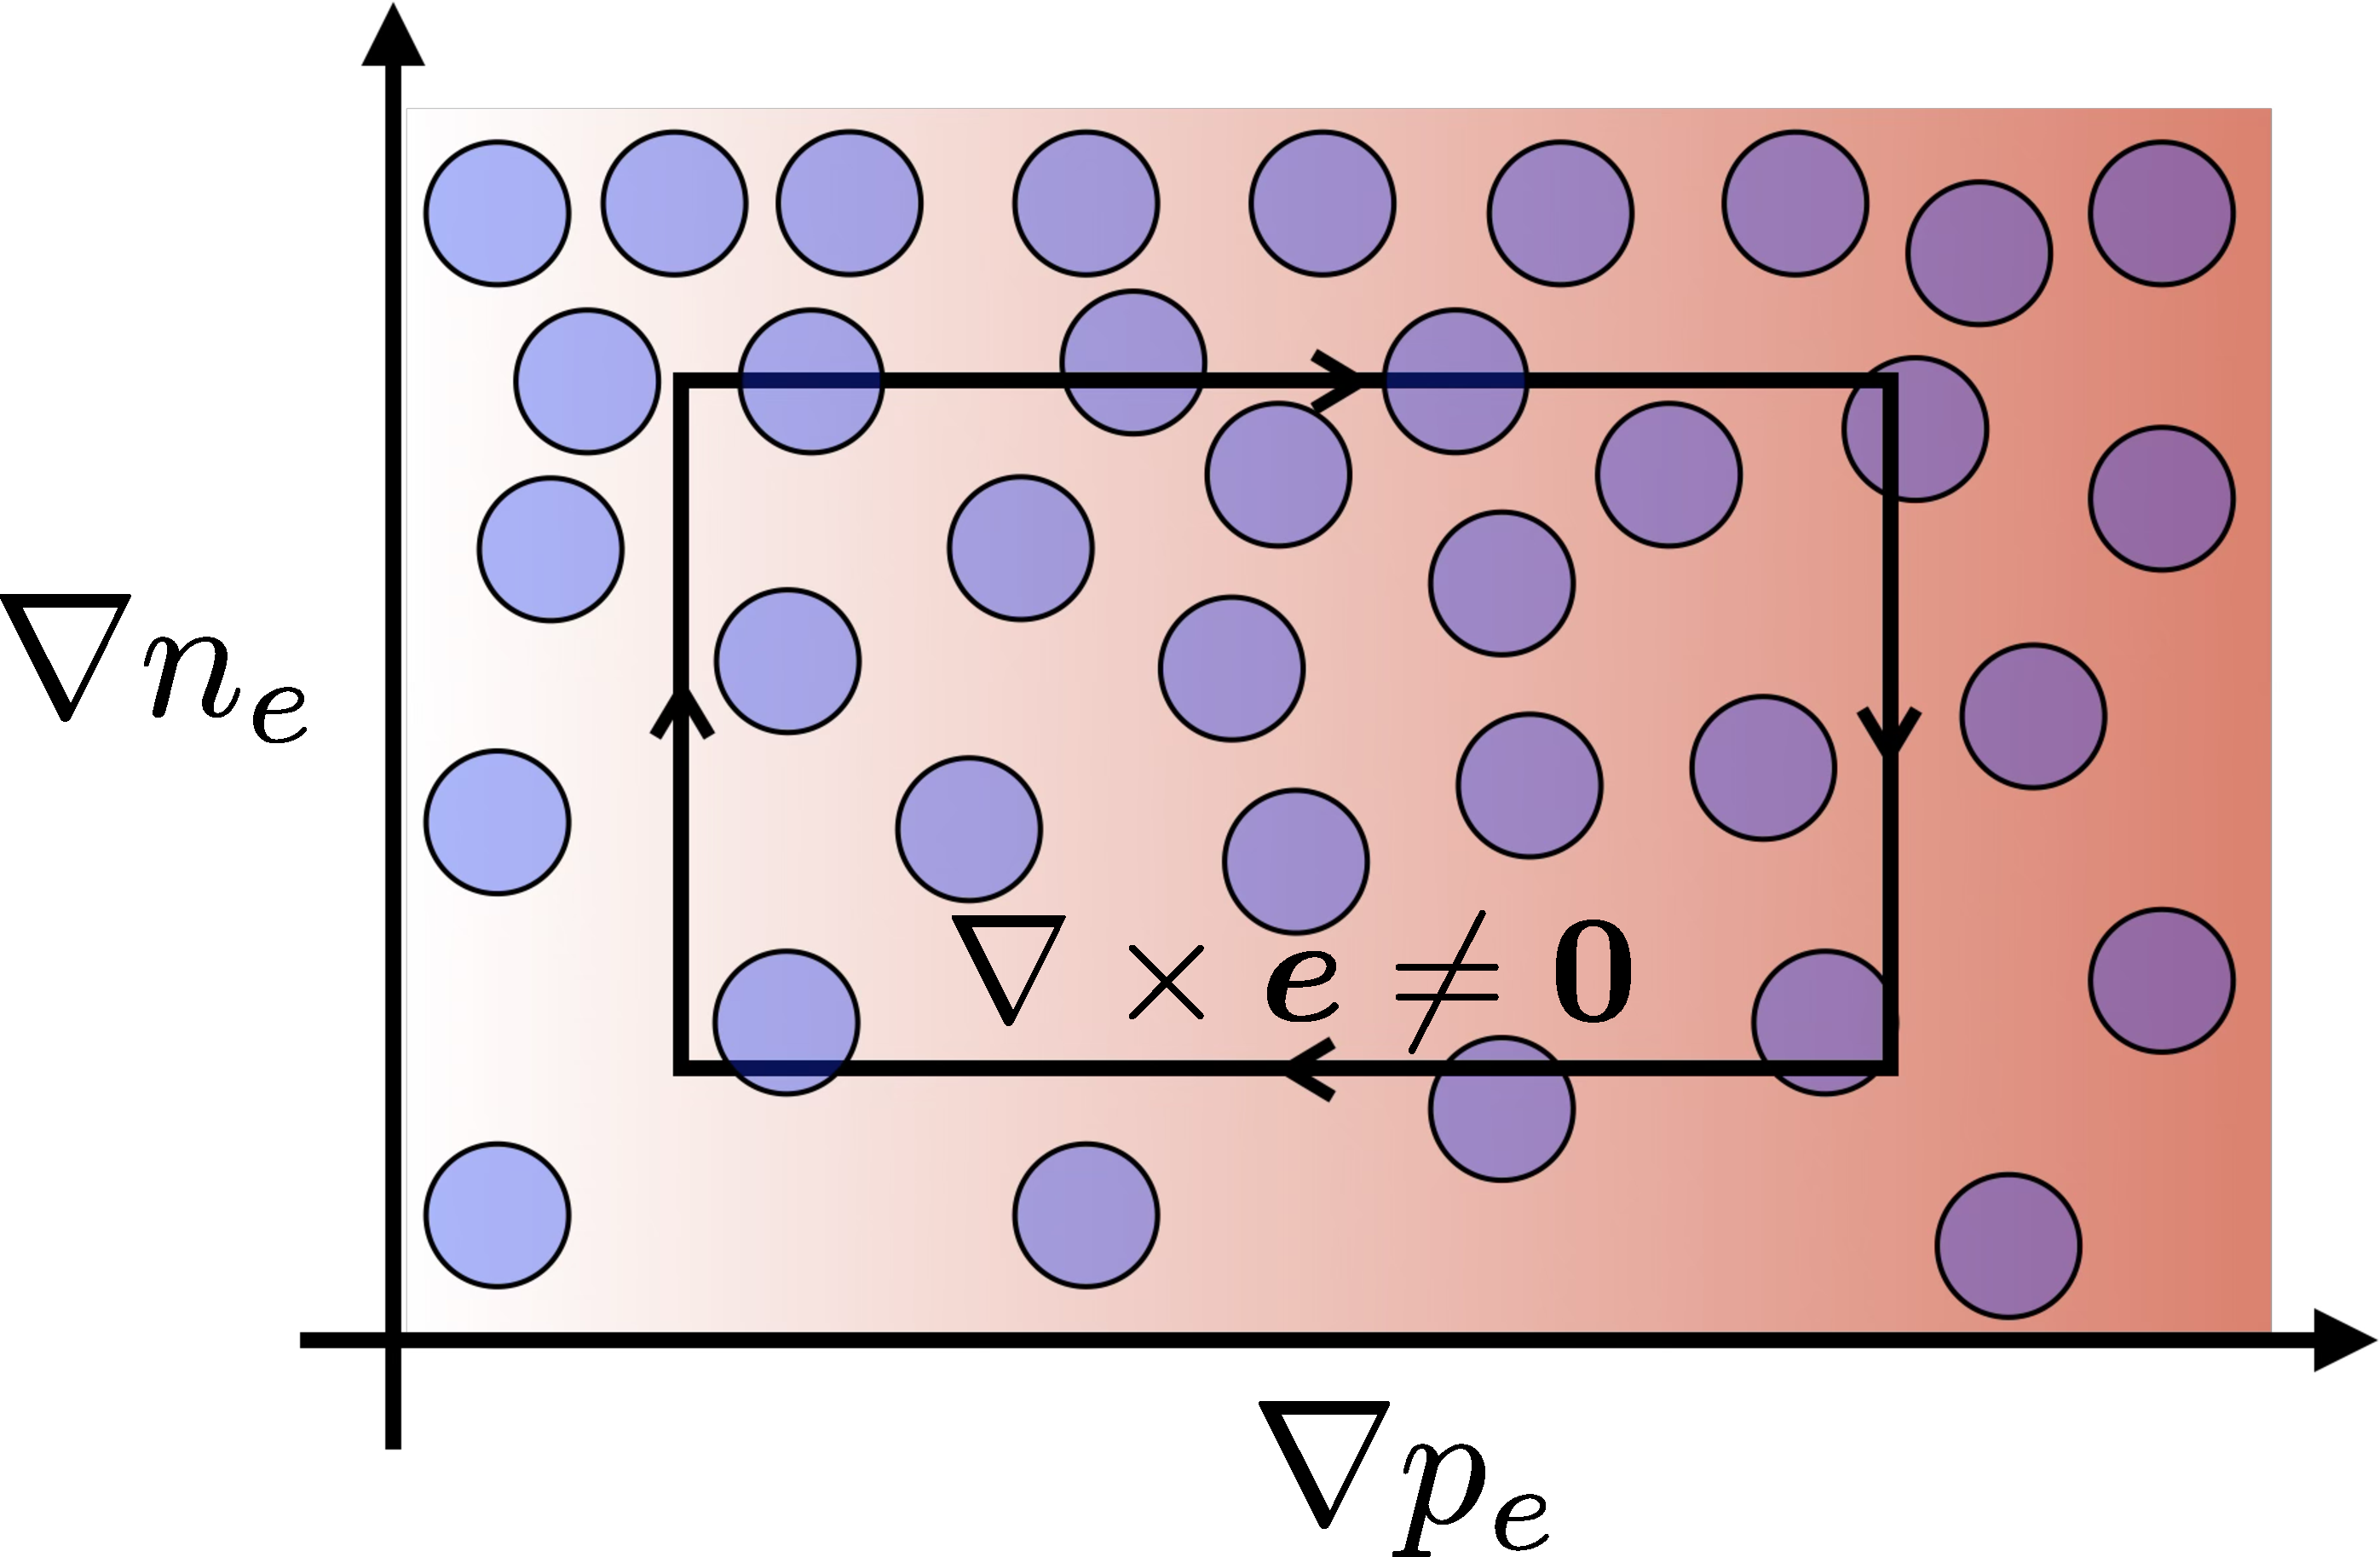
\includegraphics[width=0.65\linewidth]{figures/introduction/biermann.pdf}
    \caption{Schematic of Biermann battery seeding, adapted from a lecture by Jennifer Schober. In a baroclinic plasma, gradients in electron density and electron pressure are not aligned, so $\nabla n_e \times \nabla p_e \neq \mVector{0}$. The electron pressure term in the generalised Ohm's law then produces a non-zero curl of the electric field, $\nabla\times\mVector{e} = (1/q_e)\,(\nabla n_e \times \nabla p_e)/n_e^2$, which yields a non-zero electromotive circulation around a loop. Through Faraday's law, this drives $\partial \mVector{b}/\partial t \neq 0$ and generates a seed magnetic field even when $\mVector{b}=0$ initially.}
    \label{fig:placeholder}
\end{figure}

\citet{gnedin2000generation} was among the first to demonstrate the Biermann battery operating in a cosmological simulation, showing that baroclinic structures naturally form in the reionisation fronts surrounding protogalaxies. They found that this generates volume-filling seed fields of $b \sim 10^{-19} \,\mathrm{G}$, with stronger $b \gtrsim 10^{-18} \,\mathrm{G}$ in actively forming haloes. More recently, \citet{attia2021cosmological} and \citet{garaldi2021magnetogenesis} revisited this problem by solving the coupled radiation-MHD system self-consistently\footnote{
    \citet{gnedin2000generation} followed Biermann seeding in a decoupled, kinematic regime (see its definition in \S\ref{sec:evolve:paths}), evolving $\mVector{b}$ as a passive field. \citet{attia2021cosmological} and \citet{garaldi2021magnetogenesis} instead evolved $\mVector{b}$ self-consistently.
%DIF <  While \citet{gnedin2000generation} followed Biermann seeding in a $4 \, h^{-1} \mathrm{Mpc}$ cosmological volume (where $h$ is the dimensionless Hubble parameter) with a spatial resolution of $\sim 1 \, h^{-1} \mathrm{kpc}$, their magnetic field was evolved as a passive quantity, so, once generated, these fields could not influence the dynamics of the gas. \citet{attia2021cosmological} and \citet{garaldi2021magnetogenesis} both treated magnetic fields self-consistently, but with different numerical treatments motivated by different science goals. \citet{attia2021cosmological} developed a new constrained-transport treatment (this is the same formalism we adopt for our code \textsc{quokkka}; see \S\ref{sec:sims:ct} and Chapter bla) that included the Biermann source term, so that $\mDDiv{\mVector{b}} = 0$ is  preserved by construction (to numerical precision). Combined with adaptive refinement, they were able to reach $\sim 10\,\mathrm{pc}$ resolution in dense gas at $z \sim 6$, which enabled them to identify and separate the different conditions under which the Biermann battery operates efficiently. \citet{garaldi2021magnetogenesis} instead adopted a moving-mesh with $\mDDiv{\mVector{b}}$ controlled via Powell cleaning, which allowed them to follow the transport and reorganisation of seed $\mVector{b}$ during the collapse and assembly of galaxies.
}, confirming that reionisation fronts provide the dominant Biermann seeding channel in cosmological settings. \citet{attia2021cosmological} further showed that the net seed field receives contributions from multiple epochs, including $b \sim 10^{-25} \,\mathrm{G}$ from weak pre-reionisation seeding during linear structure growth, and $b \sim 10^{-18} \,\mathrm{G}$ in hot, shock-heated bubbles driven by stellar feedback around massive galaxies.

Focusing on the subsequent fate of these extremely weak seed fields, \citet{garaldi2021magnetogenesis} showed that the $\mVector{b}$ that ultimately threads galaxies does not retain the structural properties of its seed topology. Instead, $\mVector{b}$ is amplified during galaxy formation by a mixture of collapse-driven compression and chaotic motions that stretch and fold the field (see \S\ref{sec:evolve:paths} for a discussion on evolution channels for galactic magnetic fields), so present-day galactic fields need not resemble their original configuration. \citet{garaldi2021magnetogenesis} further found that even when $\mVector{b}$ is generated through different battery models (including \DIFdelbegin \DIFdel{a }\DIFdelend \DIFaddbegin \DIFadd{the }\DIFaddend photoionisation-driven Durrive battery \DIFaddbegin \DIFadd{\mbox{%DIFAUXCMD
\citep{durrive2015intergalactic}}\hskip0pt%DIFAUXCMD
}\DIFaddend ), the properties of $\mVector{b}$ in dense galactic gas converge toward similar states. This insensitivity to the seed mechanism is not universal, however, and the most diffuse environments remain more sensitive to their initial conditions. \citet{mtchedlidze2022evolution} investigated this explicitly by imposing different primordial seed strengths and topologies in cosmological simulations, and then following the field through large-scale structure formation. They showed that the clearest differences persist in the most rarefied regions of the cosmic web, particularly in cosmic voids. Magnetic fields in voids therefore provide one of the clearest observational tests of competing magnetogenesis scenarios.

\subsection{Flavours of Magnetic Evolution}
\label{sec:evolve}

Once $\psi_\mathrm{mag} > 0$ has been seeded, \autoref{eqn:mhd:mass}--\ref{eqn:mhd:monopoles} become sufficient to describe the evolution of magnetised plasmas. These equations admit a wide range of flow regimes, with various force terms playing different roles. It therefore becomes useful to think about the relative importance of these terms, and the kinds of dynamics they can produce. To expose this, we non-dimensionalise the evolution equations by introducing a characteristic length scale $\ell_0$, bulk velocity $u_0$, density $\rho_0,$ and magnetic amplitude $b_0$, which allow us to define dimensionless variables
\begin{align}
    \tilde{t}
        = \frac{u_0}{\ell_0} t
        , \qquad
    \tilde{\mVector{x}}
        = \frac{\mVector{x}}{\ell_0}
        , \qquad
    \tilde{\rho}
        &= \frac{\rho}{\rho_0}
        , \qquad
    \tilde{\mVector{u}}
        = \frac{\mVector{u}}{u_0}
        , \qquad
    \tilde{\mVector{b}}
        = \frac{\mVector{b}}{b_0}
        \\
    \tilde{\nabla}
        = \ell_0 \nabla
        , \qquad &\mbox{and} \qquad
    \tilde{\mTensor{V}}
        = \frac{\ell_0}{\nu \rho_0 u_0} \mTensor{V}
    .
\end{align}
Substituting these into \autoref{eqn:mhd:momentum} and setting $\mVector{f} = \mVector{0}$ (for convenience) yields the dimensionless momentum equation
\begin{align}
    \mppFrac{(\tilde{\rho} \tilde{\mVector{u}})}{\tilde{t}}
        + \tilde{\nabla} \cdot \rbrac{
            \tilde{\rho} (\tilde{\mVector{u}} \otimes \tilde{\mVector{u}})
            + \frac{1}{\mSonicMach^2} \tilde{\rho} \mTensor{I}
            + \frac{1}{\mAlfvenMach^2} \rbrac{
                \frac{\tilde{b}^2}{2} \mTensor{I}
                - \tilde{\mVector{b}} \otimes \tilde{\mVector{b}}
            }
            + \frac{\tilde{\mTensor{V}}}{\mReh}
        }
        = 0
    ,
\end{align}
where
\begin{align}
    \mSonicMach
        \equiv \frac{u_0}{c_s}
        , \qquad
    \mAlfvenMach
        \equiv \frac{\sqrt{4\pi\rho_0} u_0}{b_0}
        , \qquad \mbox{and} \qquad
    \mReh
        \equiv \frac{u_0\ell_0}{\nu}
        \sim \frac{
            \|\nabla\cdot(\rho\,\mVector{u}\otimes\mVector{u})\|
        }{
            \|\nabla\cdot\mTensor{V}\|
        }
    ,
    \label{defn:Reh}
\end{align}
measure the degree of compressibility, the relative importance of inertial to magnetic stresses, and the relative importance of inertial to viscous stresses (see \S\ref{sec:evolve:ssd}), respectively. It is also useful to compare the relative thermal and magnetic pressure reservoirs, which is captured by
\begin{align}
    \beta
        \equiv 2 \rfrac{\mAlfvenMach}{\mSonicMach}^2
    , \label{defn:plasma-beta}
\end{align}
and indicates when flows are magnetically dominated ($\beta \ll 1$), and conversely when they are hydrodynamically dominated ($\beta \gg 1$).

Similarly, when we non-dimensionalise \autoref{eqn:mhd:induction},
\begin{align}
    \mppFrac{\tilde{\mVector{b}}}{\tilde{t}}
        = \tilde{\nabla} \times \rbrac{\tilde{\mVector{u}}\times\tilde{\mVector{b}}}
            + \frac{1}{\mRem}\,\tilde{\nabla}^2 \tilde{\mVector{b}}
        ,
\end{align}
we are introduced to
\begin{align}
    \mRem
        \equiv \frac{u_0\ell_0}{\eta}
        \sim \frac{
                \|\nabla\times(\mVector{u}\times\mVector{b})\|
            }{
                \|\mCurl{(\eta\mCurl{\mVector{b}})}\|
            }
    ,
    \label{defn:Rem}
\end{align}
which measures the relative importance of inductive advection to resistive diffusion (see \S\ref{sec:evolve:decay}).

\begin{figure}
    \centering
    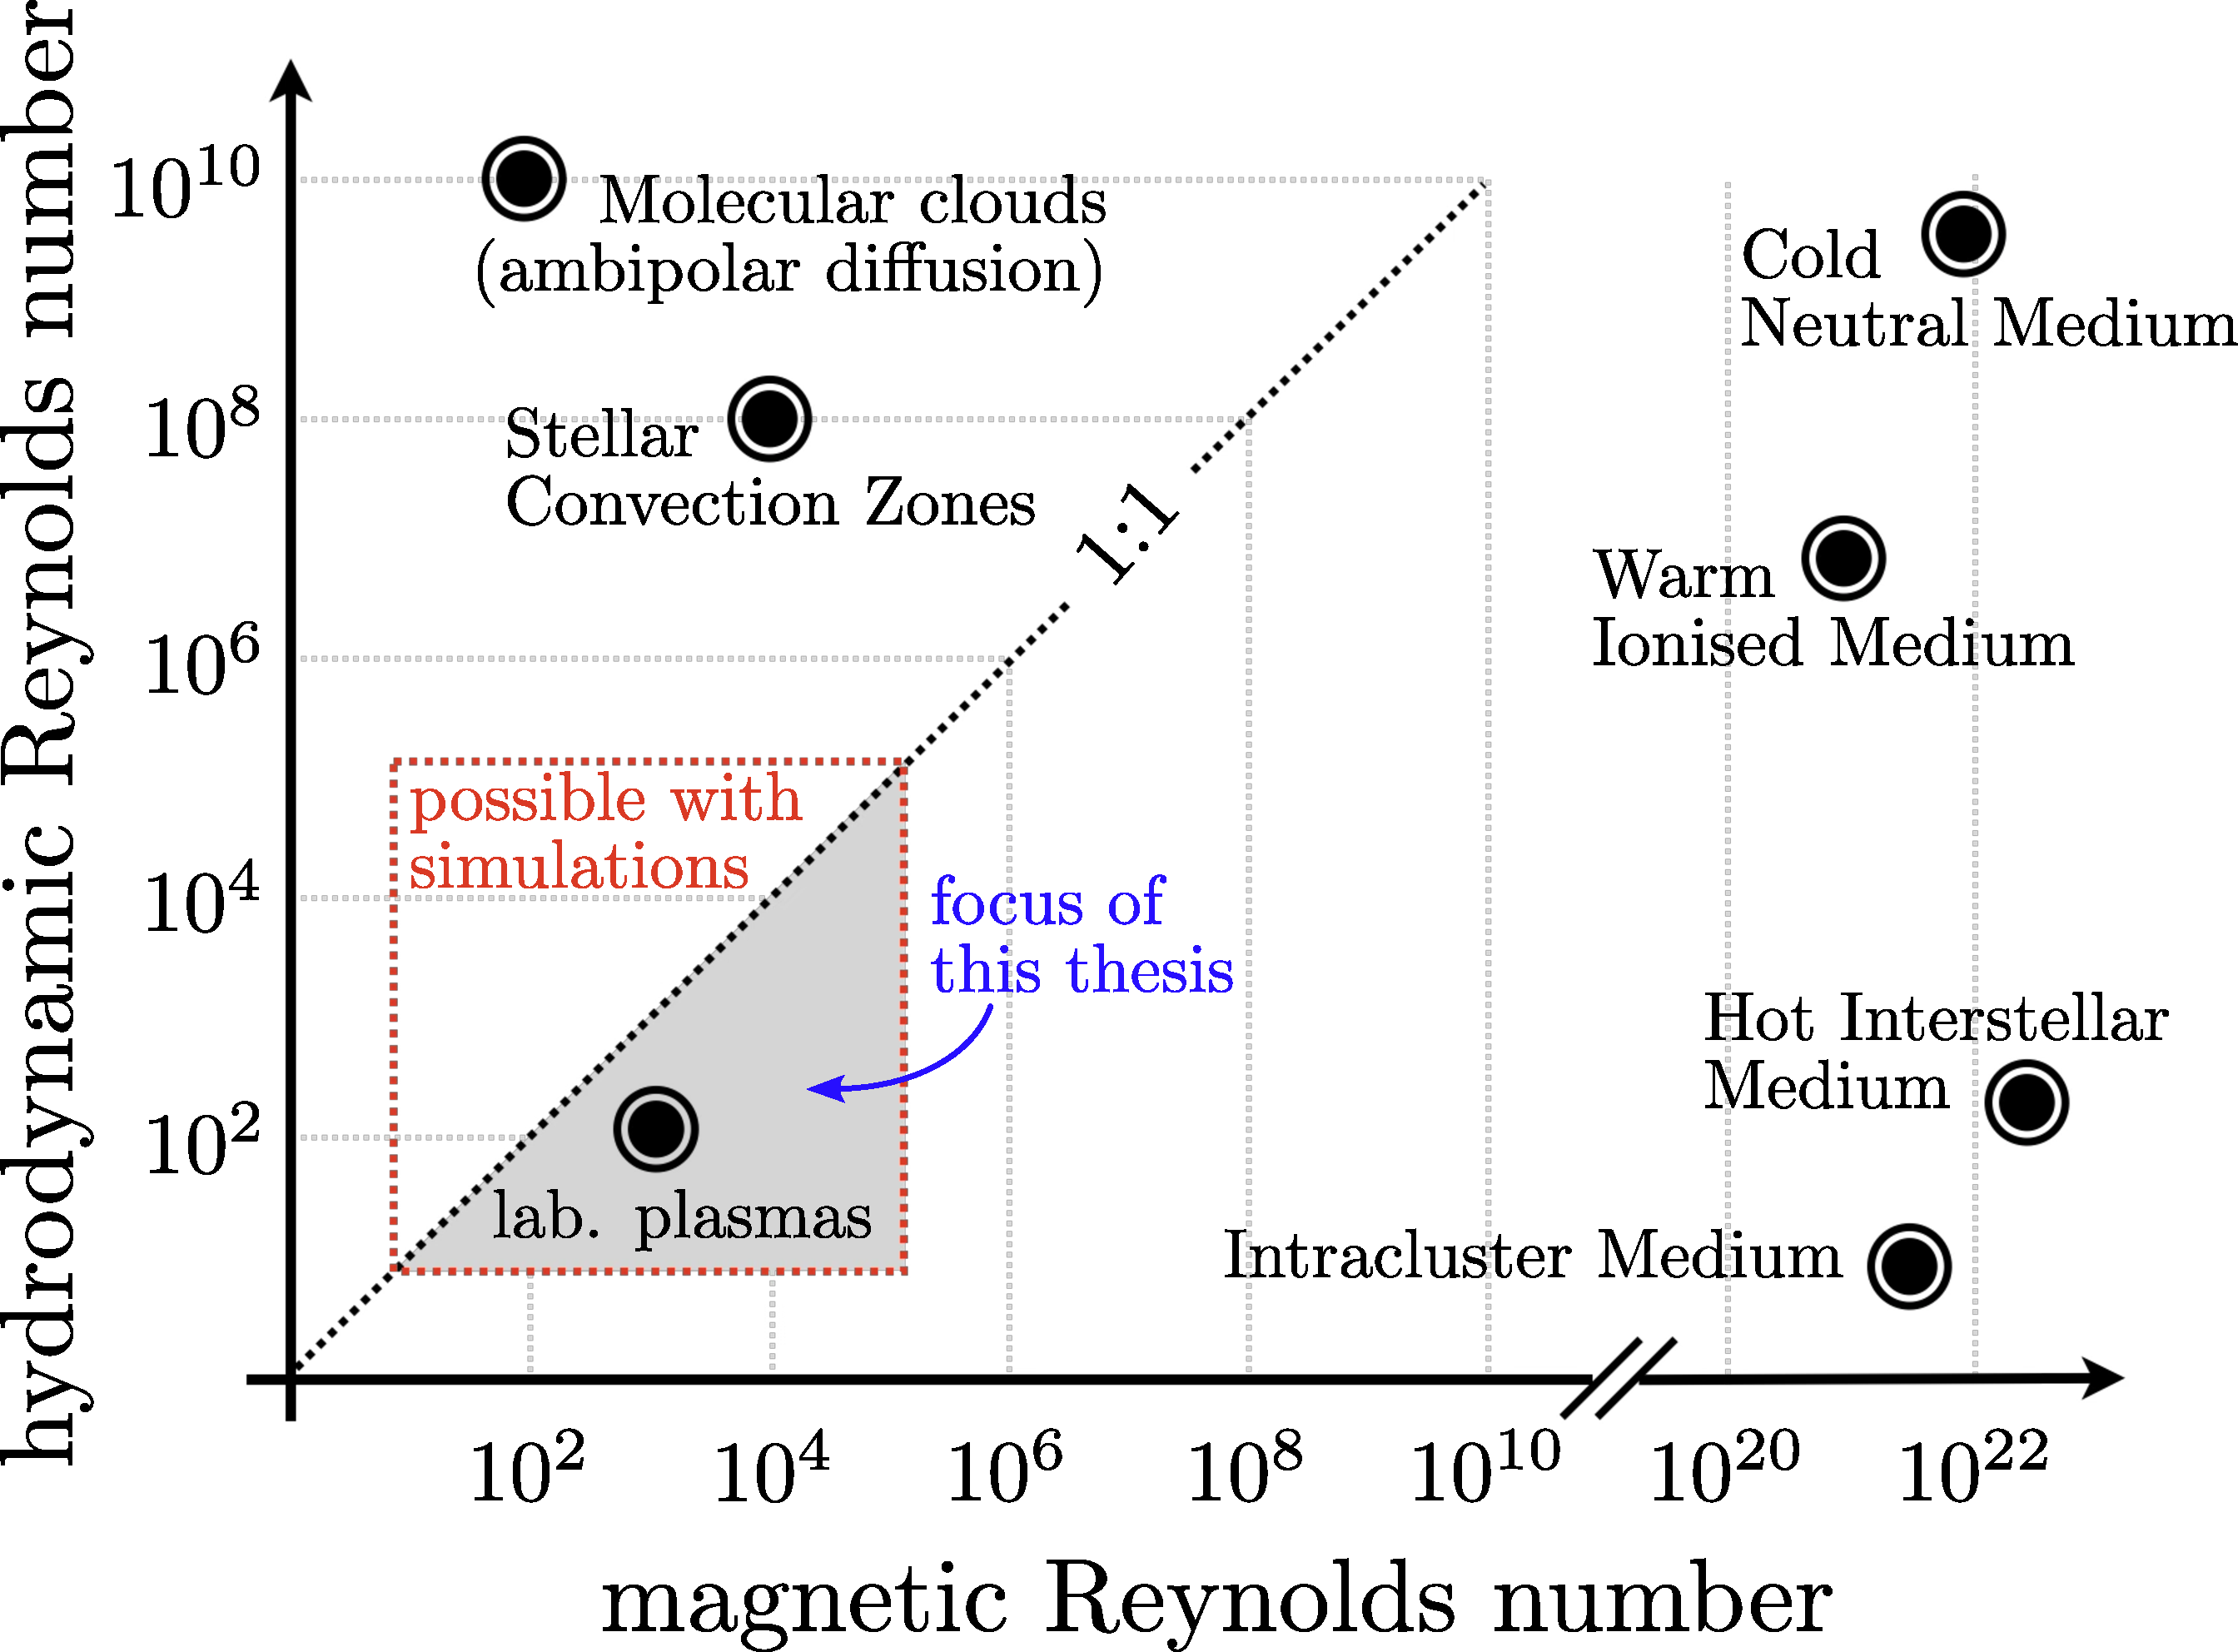
\includegraphics[width=0.8\linewidth]{figures/introduction/regimes.pdf}
    \caption{Order-of-magnitude hydrodynamic (\autoref{defn:Reh}) and magnetic Reynolds numbers (\autoref{defn:Rem}) for a representative selection of astrophysical environments, using parameters compiled from \citet{rincon2019dynamo} and \citet{brandenburg2023galactic}. These two dimensionless numbers are among the key parameters that diagnose the relative importance of different dynamical processes (see also \autoref{defn:plasma-beta}). A diagonal dotted line shows $\mathrm{Pm} = 1$ (see \autoref{defn:Prm}), for which viscous and resistive dissipation take place on comparable scales. Separately, the red box indicates the region of this parameter space that is currently accessible to direct numerical simulations; for the time being, most realistic astrophysical plasmas remain far out-of-reach, but simulations can nevertheless probe the consequences of different dynamical effects. The grey triangle highlights the subset of this accessible space that is the focus of this thesis.}
    \label{fig:plasma-regimes}
\end{figure}

As \citet{rincon2019dynamo} summarises nicely in a schematic much like \autoref{fig:plasma-regimes}, astrophysical plasmas span a vast range of configurations in the parameter space defined by $\mReh$ and $\mRem$, which are often enormous. In these inertial and inductive dominated flow regimes, it is the relative (rather than absolute) magnitudes of these two numbers that becomes relevant, with the magnetic Prandtl number
\begin{align}
    \mPrm
        &= \frac{\mRem}{\mReh}
        \sim \frac{\nu}{\eta}
    , \label{defn:Prm}
\end{align}
providing a convenient measure of the separation between viscous and resistive effects. In this thesis we exclusively focus on the $\mPrm \geq 1$ regime, which is relevant for many diffuse astrophysical plasmas, including the $\mSonicMach \gtrsim 1$, $\mReh \gg 1$ turbulence in the interstellar medium, where galactic magnetic fields are thought to be maintained.

\subsubsection{The Dynamical Roads Along Which Magnetism Walks}
\label{sec:evolve:paths}

One of the key takeaways from our discussion of magnetogenesis in \S\ref{sec:modelling:magnetogenesis} is that, while there are many plausible mechanisms capable of seeding the first magnetic fields, none produced the fields we observe in the present-day Universe (\eg those discussed in \S\ref{sec:what-we-see}) in their present form. For one, seed fields are far weaker than the magnetic fields we infer today. The magnetic fields we see, whether on the scales of molecular clouds in the interstellar medium, or threading galactic discs and halos, must therefore have undergone substantial amplification and reorganisation ever since they were seeded.

For much of this magnetic history, galactic fields are expected to have been dynamically weak compared to the motions of the gas, $\psi_\mathrm{mag} \ll \psi_\mathrm{kin}$. In this limit, Lorentz forces become negligible in \autoref{eqn:mhd:momentum}, so, as far as the momentum budget is concerned, the gas evolves as if it were effectively unmagnetised. To leading order, \autoref{eqn:mhd:momentum} therefore reduces back to its hydrodynamic form,
\begin{align}
    \mppFrac{(\rho \mVector{u})}{t}
        + \nabla \cdot \rbrac{
            \rho \mVector{u}\otimes\mVector{u}
            + p \mTensor{I}
            - \mTensor{V}
        }
        &= \rho \mVector{f}
    .
\end{align}
With this, $\mVector{u}$ evolves independently of $\mVector{b}$, and \autoref{eqn:mhd:induction} becomes linear in $\mVector{b}$. It follows that the instantaneous fractional evolution of magnetic energy density,
\begin{align}
    \mDDFrac{(\ln\psi_\mathrm{mag})}{t}
        = \frac{1}{\psi_\mathrm{mag}} \mDDFrac{\psi_\mathrm{mag}}{t}
        = \frac{2\mVector{b}}{b^2} \cdot \mDDFrac{\mVector{b}}{t}
    ,
\end{align}
does not depend on the magnitude of $\psi_\mathrm{mag}$; here $\mDD / \mDD t \equiv \partial/\partial t + \mVector{u}\cdot\nabla$ is the material derivative. This flow regime is popularly referred to as \textit{kinematic}.

\begin{figure}
    \centering
    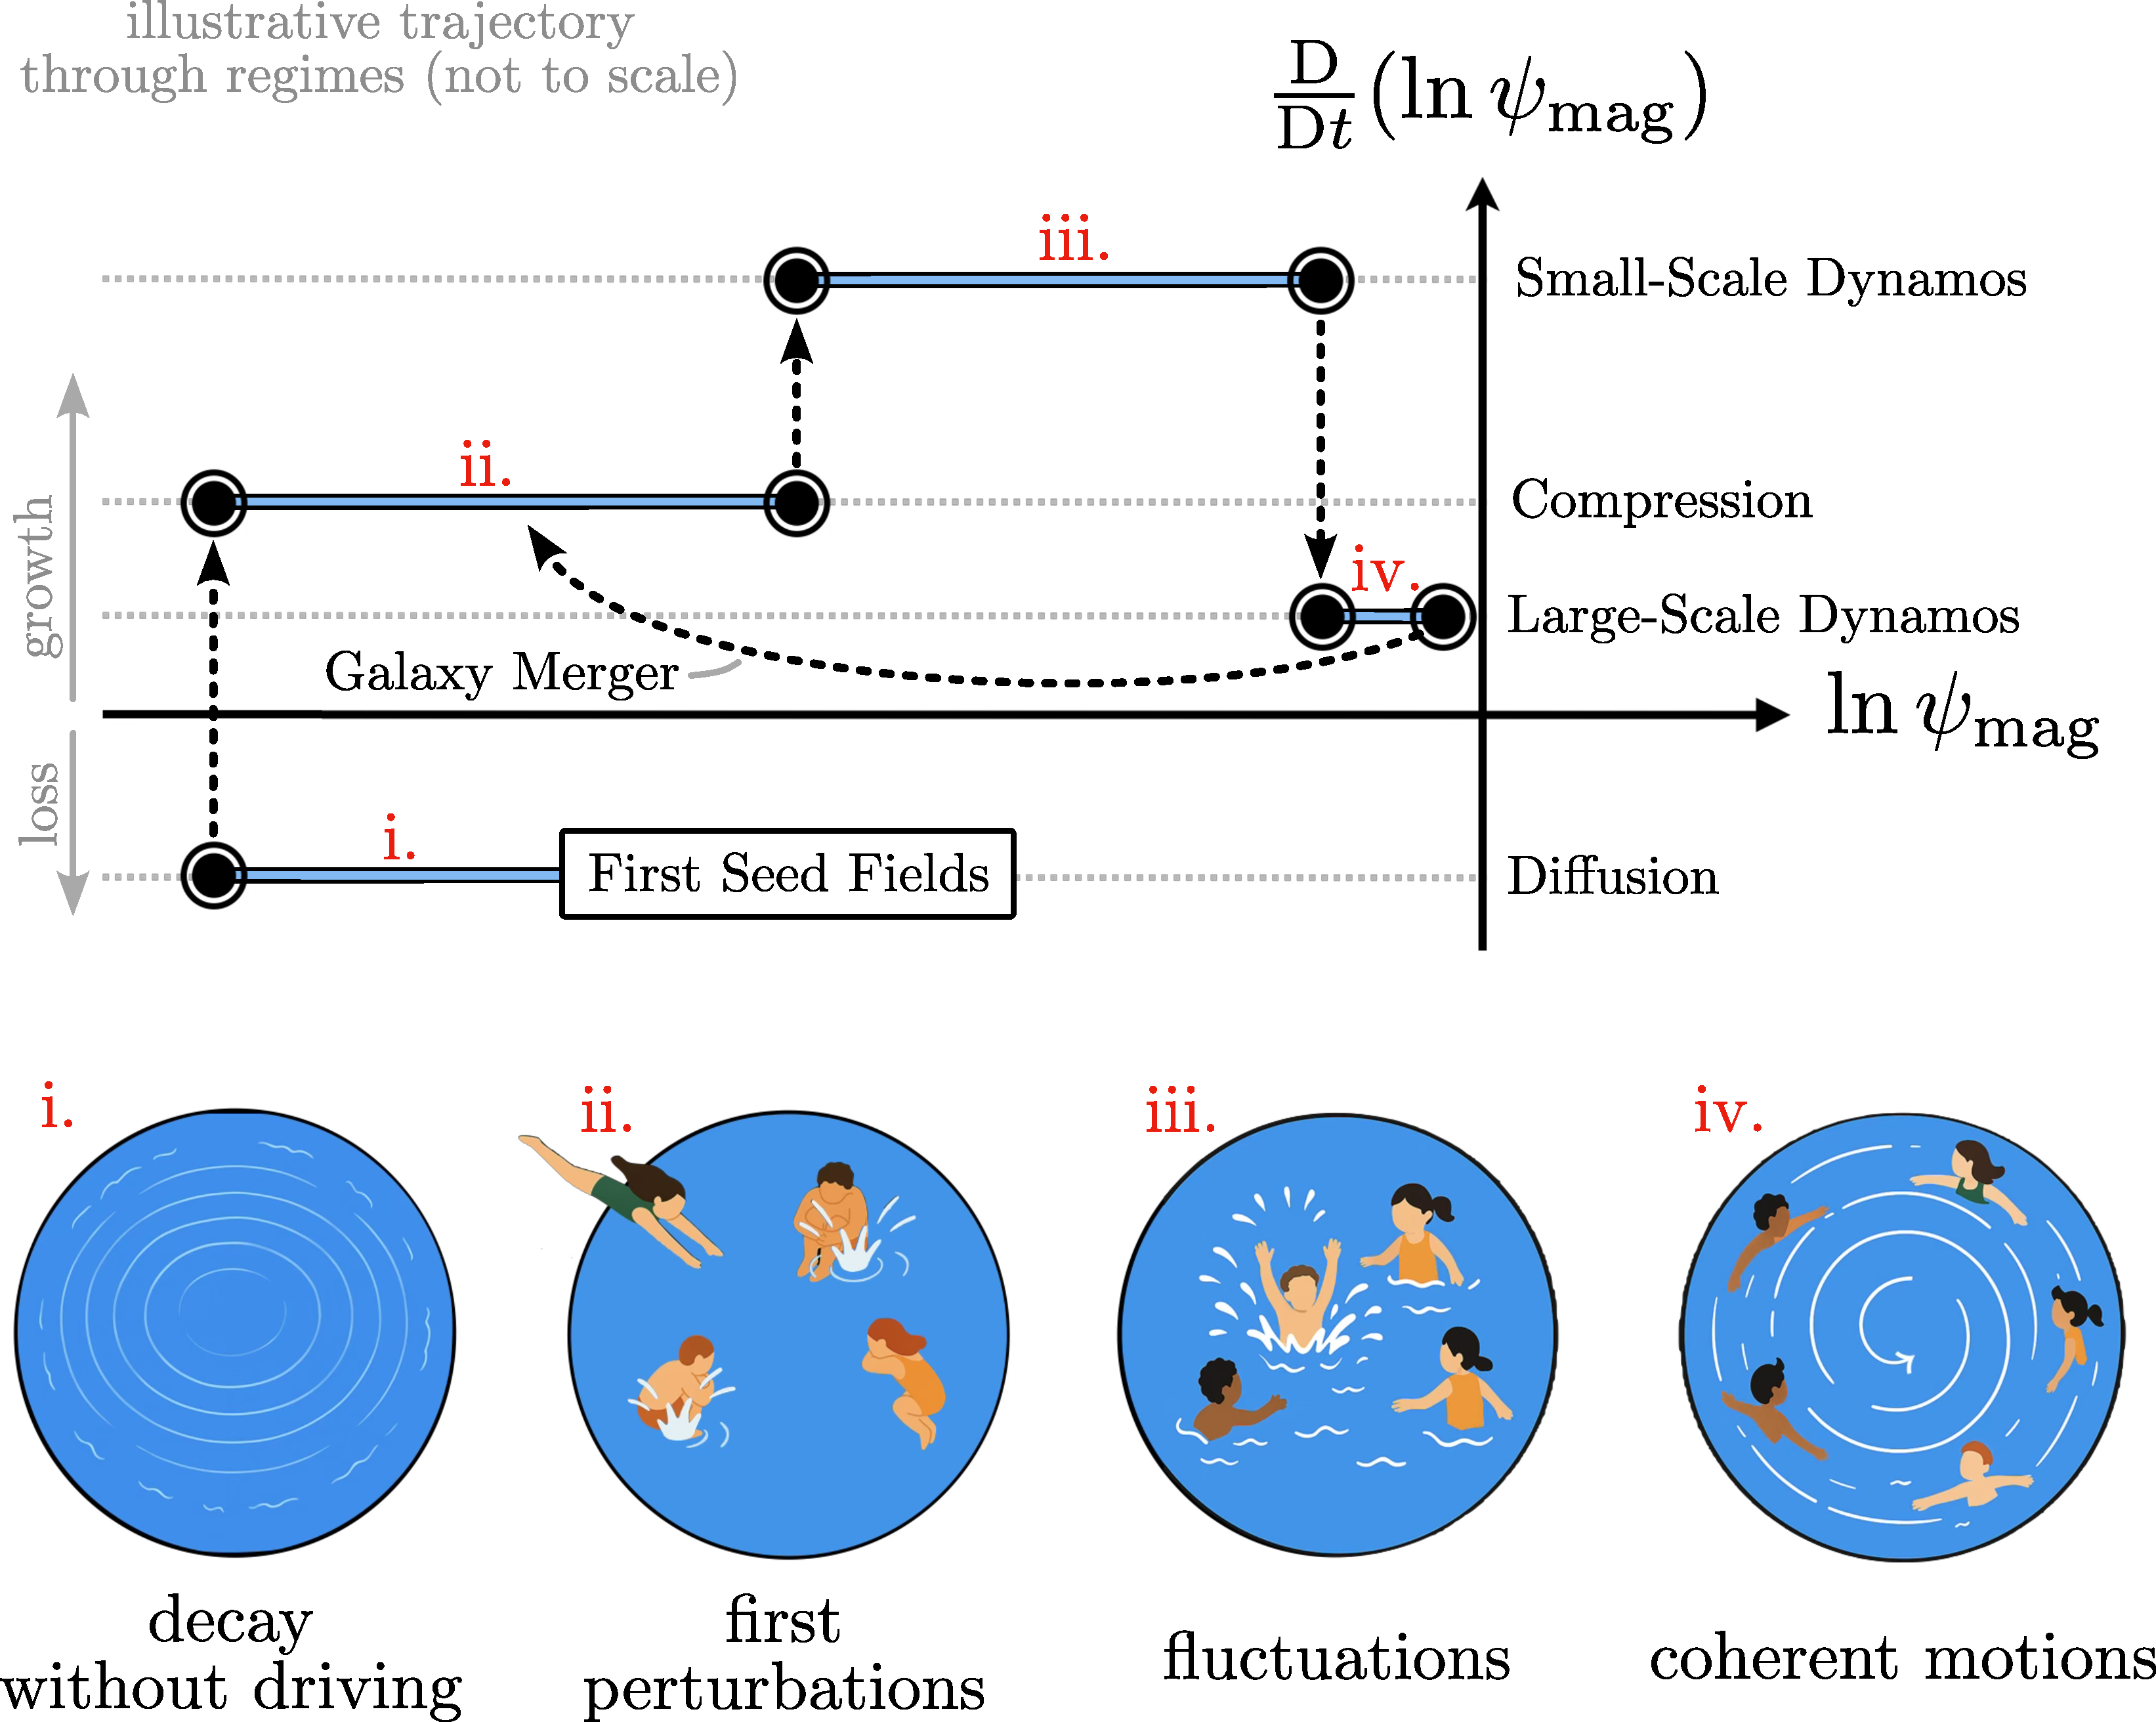
\includegraphics[width=\linewidth]{figures/introduction/dynamical.pdf}
    \caption{Schematic illustration of magnetic evolution channels (top), shown in terms of the log-transformed field strength $\ln\psi_\mathrm{mag}$ and its instantaneous fractional growth rate $\mathrm{D}(\ln\psi_\mathrm{mag}) / \mathrm{D}t$, together with a pool analogy (bottom). In the analogy, water represents magnetic fields in a plasma, and waves represent magnetic energy; it is \textit{currents} in the water that direct how waves are transported. (i) in the absence of active wave generation, waves decay (diffusion); (ii) disturbances injected into the pool grow \textit{the first} waves (\S\ref{sec:modelling:magnetogenesis} and \S\ref{sec:evolve:compression}); (iii) chaotic fluctuations produce many interacting waves, with some constructive (in-phase) and some destructive (out-of-phase) contributions, yielding net growth of waves (\S\ref{sec:evolve:ssd}; this is the most efficient means to grow waves); and (iv) sustained coherent motions develop larger-scale waves (\S\ref{sec:evolve:lsd}; harder to induce in smaller pools). The numbered yellow (brick) road indicates an illustrative trajectory through these attractor channels as the flow conditions evolve (not to scale), including the possibility of returning to earlier regimes as new episodes of compression and turbulence are reintroduced.}
    \label{fig:dynamical}
\end{figure}

The velocity field to which $\mVector{b}$ is subjected in this kinematic regime is not constant through cosmic time. As a galaxy assembles, gas first collapses into haloes and filaments, with radiative cooling and feedback driving the interstellar medium into a turbulent, multiphase state, and, in large Milky Way-like galaxies, long-lived rotation develops a coherent disc. Moreover, for large galaxies like our Milky Way, this path is not travelled just once. Instead, galaxy assembly happens through repeated mergers, which reintroduce strong compression and turbulence, and disrupt coherent rotation-driven structures, pushing the magnetic system back toward earlier flow conditions. Each epoch of magnetic field evolution reshuffles which terms in \autoref{eqn:mhd:momentum} and \autoref{eqn:mhd:induction} dominate, and moves the field onto different evolutionary channels. In \autoref{fig:dynamical} we summarise these channels and the transitions between them. In the remainder of this section we describe these channels in turn, beginning with diffusion (\S\ref{sec:evolve:decay}) and compression (\S\ref{sec:evolve:compression}), before turning to small-scale and large-scale dynamo action (\S\ref{sec:evolve:ssd} and \S\ref{sec:evolve:lsd}, respectively).

\subsubsection{Diffusion}
\label{sec:evolve:decay}

One of the first things one should notice about the induction equation, \autoref{eqn:mhd:induction}, is that it contains two competing terms. The first is inductive stretching, which couples magnetic fields to the flow, and, in the ideal limit ($\eta \to 0$), leaves them to advect flux-frozen\footnote{
    For an arbitrary material surface $\mSurface(t)$ advecting with velocity $\mVector{\chi}$, the Leibniz-Reynolds transport theorem gives
    \begin{align}
    \mppFrac{}{t} \int_{\mSurface(t)} \mVector{\xi} \cdot\mdd\mVector{S}
        &= \int_{\mSurface(t)} \sbrac{
                \mppFrac{\mVector{\xi}}{t}
                - \nabla\times(\mVector{\chi}\times\mVector{\xi})
            }\cdot\mdd\mVector{S}
        .
    \end{align}
    From this statement, it then follows that if $\mVector{\xi}$ evolves according to $\mpp_t\mVector{\xi} = \nabla\times(\mVector{\chi}\times\mVector{\xi})$, then its flux through any material surface is conserved and its topology is frozen into the medium. This condition is satisfied for ideal MHD, since $\mVector{\xi} = \mVector{b}$ obeys this induction form with $\mVector{\chi} = \mVector{u}$.
    \label{fnote:frozen}
} in the gas. The second term is diffusion, which is the inevitable consequence of real plasmas not being perfectly conducting ($\eta$ remains finite). Diffusion provides the default evolutionary channel whenever a flow does not continually regenerate magnetic structure, with the magnetic Reynolds number ($\mRem$; \autoref{defn:Rem}) providing a useful metric for when diffusion can compete with induction on a given scale. In many astrophysical environments $\mRem \gg 1$ on the largest coherent scales, but as the field is driven into smaller-scale structure, gradients sharpen and diffusion can become dynamically important.

The consequence of this is that, unless there exists a flow to stretch and produce magnetic structure, diffusion will act to remove it. In particular, this happens when $\mVector{u} \approx \mVector{0}$, or in the special case where $\mVector{u}\parallel\mVector{b}$, the induction term turns off. In these limits, \autoref{eqn:mhd:induction} reduces to a diffusion equation (assuming $\eta$ constant in space),
\begin{align}
    \mDDFrac{\mVector{b}}{t}
        \sim \eta \nabla^2 \mVector{b}
    .
\end{align}
Magnetic fields therefore decay through resistive diffusion on a characteristic timescale
\begin{align}
    t_\eta
        \sim \frac{\ell_0^2}{\eta}
        \sim \mRem \frac{\ell_0}{u_0}
    .
\end{align}

For the Earth's magnetic field, which is associated with convective motions on $\ell_0 \sim 3\times 10^8~\mathrm{cm}$ in the liquid outer core, with diffusivity $\eta \sim 10^4 \,\mathrm{cm}^2 \,\mathrm{s}^{-1}$, this predicts a decay time of $t_\eta \sim 3 \times 10^5~\mathrm{yr}$ \citep{choudhuri1998physics}, which is much shorter than the age of the Earth. This field, therefore, cannot be a fossil from magentogenesis, since any field produced alongside the Earth would have decayed by now.

If we make a similar estimate for galactic magnetic fields, we instead predict a decay time that is significantly longer than the age of the Universe. At first, one may interpret this to mean that diffusion is not relevant for galactic fields, but this conclusion is misinformed. Unlike the comparatively coherent flows relevant for the Earth, interstellar flows are not coherent. Gas in the ISM is continually stirred by supernovae and violent outflows, which generate sharp gradients and thin current layers on small scales where dissipation becomes more efficient. In this regime, decay is not well described by smooth Ohmic diffusion, which predicts $\psi_\mathrm{mag} \propto \exp(-t/t_\eta)$. Instead, the field is actively reorganised by nonlinear dynamics\footnote{
    I refer the interested reader to \citet{schekochihin2022mhd} Section~12 for a thorough review.
}, with magnetic energy selectively decayed through the formation and reconnection of small-scale structures, even at very large $\mRem$, yielding dynamical decay $\psi_\mathrm{mag} \propto t^{-p}$ with $p \sim \mathcal{O}(1)$ \citep[see \eg][]{hosking2021reconnection}. Thus magnetic erosion in the ISM is far more efficient than the naive estimate would suggest \citep{brandenburg2025turbulent}, and the presence of magnetic structure throughout the ISM therefore leads to the same conclusion as magnetic fields here on Earth, namely that it requires sustained induction.

\subsubsection{Compression}
\label{sec:evolve:compression}

Structure formation provided the first route for seed fields to grow. As baryons collapsed into the first bound objects, converging flows concentrated magnetic flux and amplified $\psi_\mathrm{mag}$. This follows directly from \autoref{eqn:mhd:induction} in the ideal (flux-frozen; see Footnote~\ref{fnote:frozen}) limit, rewritten in Lagrangian form,
\begin{align}
    \mDDFrac{\mVector{b}}{t}
        = (\mVector{b}\cdot\nabla) \mVector{u}
            - (\nabla\cdot\mVector{u}) \mVector{b}
    .
\end{align}
The continuity equation can also be rewritten in this form,
\begin{align}
    \frac{D\rho}{Dt}
        = -\rho \, (\nabla\cdot\mVector{u})
    ,
\end{align}
from which it follows that
\begin{align}
    \mDDFrac{}{t} \rfrac{\mVector{b}}{\rho}
        = \frac{1}{\rho} \mDDFrac{\mVector{b}}{t}
            - \frac{\mVector{b}}{\rho^2} \mDDFrac{\rho}{t}
        = \rbrac{\frac{\mVector{b}}{\rho}\cdot\nabla} \mVector{u}
    ,
\end{align}
and we learn that changes in $\mVector{b} / \rho$ can only arise from velocity gradients along $\mVector{b}$. Compression along $\mVector{b}$ does not change the field strength, whereas compression in directions perpendicular to $\mVector{b}$ concentrates magnetic flux and increases the magnetic field-line density.

For isotropic spherical collapse this implies $b \propto \rho^{2/3}$, and thus $\psi_\mathrm{mag} \propto \rho^{4/3}$, with
\begin{align}
    \mDDFrac{(\ln\psi_\mathrm{mag})}{t}
        = \frac{4}{3} \mDDFrac{(\ln\rho)}{t}
        = -\frac{4}{3} \nabla\cdot\mVector{u}
    .
\end{align}
Ultimately, this growth ends once thermal pressure, turbulent motions, and eventually magnetic stresses provide support against gravity. Turbulent fluctuations, however, can nevertheless continue to amplify $\psi_\mathrm{mag}$, as we will show in the next two sections.

\subsubsection{Large Scale Dynamos}
\label{sec:evolve:lsd}

\S\ref{sec:evolve:decay} revealed a key asymmetry between hydrodynamic and MHD systems\DIFaddbegin \DIFadd{, though not simply that $\mVector{b}$ decays}\DIFaddend : once $\psi_\mathrm{mag} > 0$, resistive diffusion provides an unavoidable channel for magnetic energy to be removed, \DIFdelbegin \DIFdel{whereas in hydrodynamics there is no analogous field that decays simply by existing}\DIFdelend \DIFaddbegin \DIFadd{but temperature and other passive scalars are smoothed out by diffusion too. The real asymmetry follows from how each field grows. The induction equation contains a term linear in $\mVector{b}$ itself, stretching, which lets a seed field amplify purely by feeding on the flow's kinetic energy; no such term exists for a passive scalar, whose value can only be redistributed by advection and smoothed by diffusion}\DIFaddend . For systems like galaxies, stars, and planets, where we see magnetic fields in stable, long-lived states, the question then becomes what conditions support them. Diffusion provides one side of the answer, and growth via induction provides the other. However, anti-dynamo theorems by \citet{cowling1933magnetic} and \citet{zil1957magnetic} showed that only some fluid motions can produce dynamos; they ruled out both axisymmetric and purely planar (two-dimensional) flows. The takeaway, then, is that we should not expect overly simple, effectively two-dimensional, or highly symmetric flows to support persistent $\psi_\mathrm{mag} > 0$. Sustained magnetism requires flows with enough geometric complexity to continually regenerate the components of the field that diffusion erodes. Since Cowling and Zel'dovich, many possible dynamo scenarios have been identified (see the recent excellent reviews by, \eg \citealt{rincon2019dynamo} and \citealt{brandenburg2023galactic}). Here we focus on the standard mean-field picture relevant for Milky Way-like galaxies, and (following similar arguments in \eg \citealt{choudhuri1998physics} and \citealt{rincon2019dynamo}) show how it can generate and sustain a large-scale magnetic field.

In galaxies, radio synchrotron observations reveal magnetic structure on a wide range of scales. Polarised emission traces an ordered component that is coherent across the disc on $L \sim \mathrm{kpc}$ scales, while Faraday rotation measures indicate the presence of fluctuations on smaller $\ell_0 \sim 100 \mathrm{pc}$ scales. It then, perhaps, feels natural to decompose the galactic magnetic field into a large-scale mean component $\bar{\mVector{b}}$, describing the component of the field coherent on galactic scales $L$, and a fluctuating component $\delta\mVector{b}$, for the small-scale fluctuations about this mean on scales $\ell_0$, where $\ell_0 \ll L$. We can do the same decomposition for the velocity field, $\mVector{u} = \bar{\mVector{u}} + \delta\mVector{u}$, which, when substituted into \autoref{eqn:mhd:induction} and averaged over intermediate scales $\ell \in [\ell_0, \,L]$ (using Reynolds averaging rules), yields
\begin{align}
    \overline{\mppFrac{\mVector{b}}{t}}
        =  \mppFrac{\bar{\mVector{b}}}{t}
        = \mCurl{\rbrac{
            \bar{\mVector{u}} \times \bar{\mVector{b}}
            + \overline{\delta\mVector{u} \times \delta\mVector{b}}
            - \eta \mCurl{\bar{\mVector{b}}}
        }}
        . \label{eqn:lsd:average}
\end{align}
The companion evolution equation for magnetic fluctuations, is then
\begin{align}
    \mppFrac{(\delta\mVector{b})}{t}
        &= \mppFrac{\mVector{b}}{t} - \mppFrac{\bar{\mVector{b}}}{t} \\
        &= \mCurl{\rbrac{
            \bar{\mVector{u}}\times\delta\mVector{b}
            + \delta\mVector{u}\times\bar{\mVector{b}}
            + \delta\mVector{u}\times\delta\mVector{b}
            - \overline{\delta\mVector{u}\times\delta\mVector{b}}
            - \eta \mCurl{\delta\mVector{b}}
        }}
    . \label{eqn:lsd:delta:full}
\end{align}
Notice that $\bar{\mVector{b}}$ does not only evolve based on the large-scale features of the system, but also on the fluctuations, $\delta\mVector{b}$ and $\delta\mVector{u}$, and, importantly, the average correlation between them, $\overline{\delta\mVector{u}\times\delta\mVector{b}}$. To put forward a description for how $\bar{\mVector{b}}$ can then be generated in a galaxy, we adopt typical approximation that the contribution to this correlation is dominated by the part of $\delta\mVector{b}$ produced by turbulent distortions of the slowly varying $\bar{\mVector{b}}$. In this picture, the self-interaction of fluctuations, $ \delta\mVector{u}\times\delta\mVector{b} - \overline{\delta\mVector{u}\times\delta\mVector{b}} $, is, to first order, unimportant for the component of $\delta\mVector{b}$ that feeds back into $\bar{\mVector{b}}$. Neglecting these terms reduces \autoref{eqn:lsd:delta:full} to
\begin{align}
    \mppFrac{(\delta\mVector{b})}{t}
        \approx \mCurl{\rbrac{
            \underbrace{
                \bar{\mVector{u}}\times\delta\mVector{b}
            }_\text{mean flow advects $\delta\mVector{b}$}
            + \overbrace{
                \delta\mVector{u}\times\bar{\mVector{b}}
            }^\text{\shortstack{mean field is imprinted\\ onto $\delta\mVector{b}$}}
            - \underbrace{
                \eta \mCurl{\delta\mVector{b}}
            }_\text{diffusion damps $\delta\mVector{b}$}
        }}
    , \label{eqn:lsd:delta:reduced}
\end{align}
and motivates a closure for the average electromotive force in \autoref{eqn:lsd:average}.

Since $\bar{\mVector{b}}$ varies on scales larger than the fluctuating fields, we can approximate $\overline{\delta\mVector{u} \times \delta\mVector{b}}$ via a gradient expansion of $\bar{\mVector{b}}$, which, in index notation, takes the form
\begin{align}
    (\overline{\delta\mVector{u} \times \delta\mVector{b}})_{i}
        = \alpha_{ij} \bar{b_j} - \pi_{ijk} \mppFrac{\bar{b_j}}{x_k} + \cdots
    .
\end{align}
Here, $\alpha_{ij}$ and $\pi_{ijk}$ are transport coefficients that encode the net effect of fluctuations (\eg stratification, and angular velocity). If we assume that $\delta\mVector{u}$ is approximately homogeneous and isotropic, then these tensors simplify considerably to $\alpha_{ij} = \alpha \delta_{ij}$ and $\pi_{ijk} = \eta_{\delta u} \epsilon_{ijk}$, and the expansion simplifies to
\begin{align}
    \overline{\delta\mVector{u} \times \delta\mVector{b}}
        \approx \alpha \bar{\mVector{b}} - \eta_{\delta u} \mCurl{\bar{\mVector{b}}}
    ,
\end{align}
where $\eta_{\delta u}$ is (turbulent) mixing induced diffusion\footnote{
    Consider a sugar cube in a cup. Left unstirred, it dissolves slowly through molecular diffusion, which can take many days. This process is largely inefficient, because the cube quickly surrounds itself with a sugar-rich boundary layer that throttles diffusion. If the water is stirred, however, this layer is advected away and replaced by fresh fluid, which allows the cube to dissolve more efficiently. Turbulent mixing enhances diffusion in the same way.
}. This only holds in the regime where $\delta b \ll \delta u$, but when $\delta b \sim \delta u$, then $\alpha$ will also have a dependence on $\mVector{b}$ \citep[see \eg][]{cattaneo1996nonlinear}.

With this, we now have an evolution equation for $\bar{\mVector{b}}$ in a system where a slowly varying $\bar{\mVector{u}}$ interacts with $\delta\mVector{u}$. In the context of galactic flows, the large scale flow is dominated by differential rotation, best described in cylindrical coordinates $\bar{\mVector{u}} = r \Omega(r) \hat{\mVector{\phi}}$. In this system, the evolution equation becomes
\begin{align}
    \mppFrac{\bar{\mVector{b}}}{t}
        \approx \mCurl{\rbrac{
            \overbrace{
                r \Omega \rbrac{
                    \bar{b}_z \mVectorUnit{r}
                    - \bar{b}_r \mVectorUnit{z}
                }
            }^\text{differential rotation}
            + \underbrace{
                \alpha \bar{\mVector{b}}
            }_\text{kinetic helicity}
            - \overbrace{
                (\eta + \eta_{\delta u}) \mCurl{\bar{\mVector{b}}}
            }^\text{diffusion}
        }}
    ,
\end{align}
which highlights the important, and combined role that differential rotation plays along with kinetic helicity. Differential rotation plays the role of winding magnetic field lines around the rotation axis, producing a toroidal component\footnote{
    Since $\mpp_t \bar{b}_\phi \sim r \bar{b}_r \mppFrac{\Omega}{r}$, any $\bar{b}_r$ component of $\bar{\mVector{b}}$ is ultimately stretched by differential rotation into something toroidal, $\bar{b}_\phi$.
    \label{fnote:lsd:omega}
} about the disc, which, in the absence of helicity, $\alpha \approx 0$, does not lead to a self-sustaining dynamo. This is because differential rotation cannot recover poloidal fields once $\bar{b}$ is primarily $\bar{b}_\phi$, and so the large-scale field ultimately erodes away through diffusion (in the same spirit as Cowling's theorem). Helicity importantly regenerates poloidal fields from toroidal ones\footnote{
    For an axisymmetric disc $(\mpp_\phi = 0)$, the $\alpha$-term converts toroidal fields $\bar{b}_\phi$, back into poloidal ones. To see this, recall that the radial and vertical components of the curl in cylindrical coordinates are
    \begin{align}
    \sbrac{\mCurl{(\alpha\bar{\mVector{b}})}}_r
        = -\mppFrac{(\alpha \bar{b}_\phi)}{z}
    \qquad\mbox{and}\qquad
    \sbrac{\mCurl{(\alpha\bar{\mVector{b}})}}_z
        = \frac{1}{r}\mppFrac{}{r}\sbrac{r \alpha\bar{b}_\phi}
    ,
    \end{align}
    respectively. Therefore, $\mCurl{(\alpha\bar{\mVector{b}})}$ generates $\bar{b}_r$ and $\bar{b}_z$ from gradients of $\bar{b}_\phi$.
    \label{fnote:lsd:alpha}
}, which replenishes poloidal fields for differential rotation to wind up. Together, these two processes couple to form the $\alpha$-$\Omega$ dynamo, capable of sustaining coherent galactic fields.

One way to estimate how efficiently this process can operate is to consider how quickly the $\Omega$-effect generates toroidal fields, and the $\alpha$-effect then regenerates poloidal fields (\ie how quickly the dynamo process passes through the steps of see the schematic in \autoref{fig:galaxy}). We do so by recalling that we had assumed $\bar{\mVector{b}}$ varies on scales of the system $L$, so the radial contribution of the $\alpha$-term in \autoref{eqn:lsd:average} can be estimated to be
\begin{align}
    \mppFrac{\bar{b}_r}{t}
        = \sbrac{\mCurl{(\alpha \bar{\mVector{b}})}}_r
        \sim \frac{\alpha}{L} \bar{b}_\phi
    .
\end{align}
Taking a second time derivative and substituting the rate at which the $\Omega$-term winds fields (see Footnote~\ref{fnote:lsd:omega}), gives
\begin{align}
    \mppFrac{^2 \bar{b}_r}{t^2}
        \sim \frac{\alpha}{L} \mppFrac{\bar{b}_\phi}{t}
        \sim \frac{\alpha}{L} \rbrac{r \mppFrac{\Omega}{r}} \bar{b}_r
    ,
\end{align}
which reveals an estimate for the characteristic growth rate,
\begin{align}
    \gamma
        \sim \sqrt{\frac{\alpha}{L} r \mAbs{\mppFrac{\Omega}{r}}}
    .
\end{align}
This growth rate must compete against turbulent diffusion, which damps the mean field at a rate $\sim (\eta + \eta_{\delta u}) / L^2$, with net growth only possible when
\begin{align}
    \sqrt{\alpha L^3 r \mAbs{\mppFrac{\Omega}{r}}}
        \gtrsim \eta + \eta_{\delta u}
    ,
\end{align}
where this excitation condition is usually expressed in terms of a ``dynamo number''
\begin{align}
    \mathcal{D}
        \equiv \frac{
                L^3 \alpha r \mAbs{\mpp_r \Omega}
            }{
                (\eta + \eta_{\delta u})^2
            }
    ,
\end{align}
with large-scale growth expected when $\mathcal{D} \gtrsim \mathcal{O}(1 - 10)$.

\begin{figure}
    \centering
    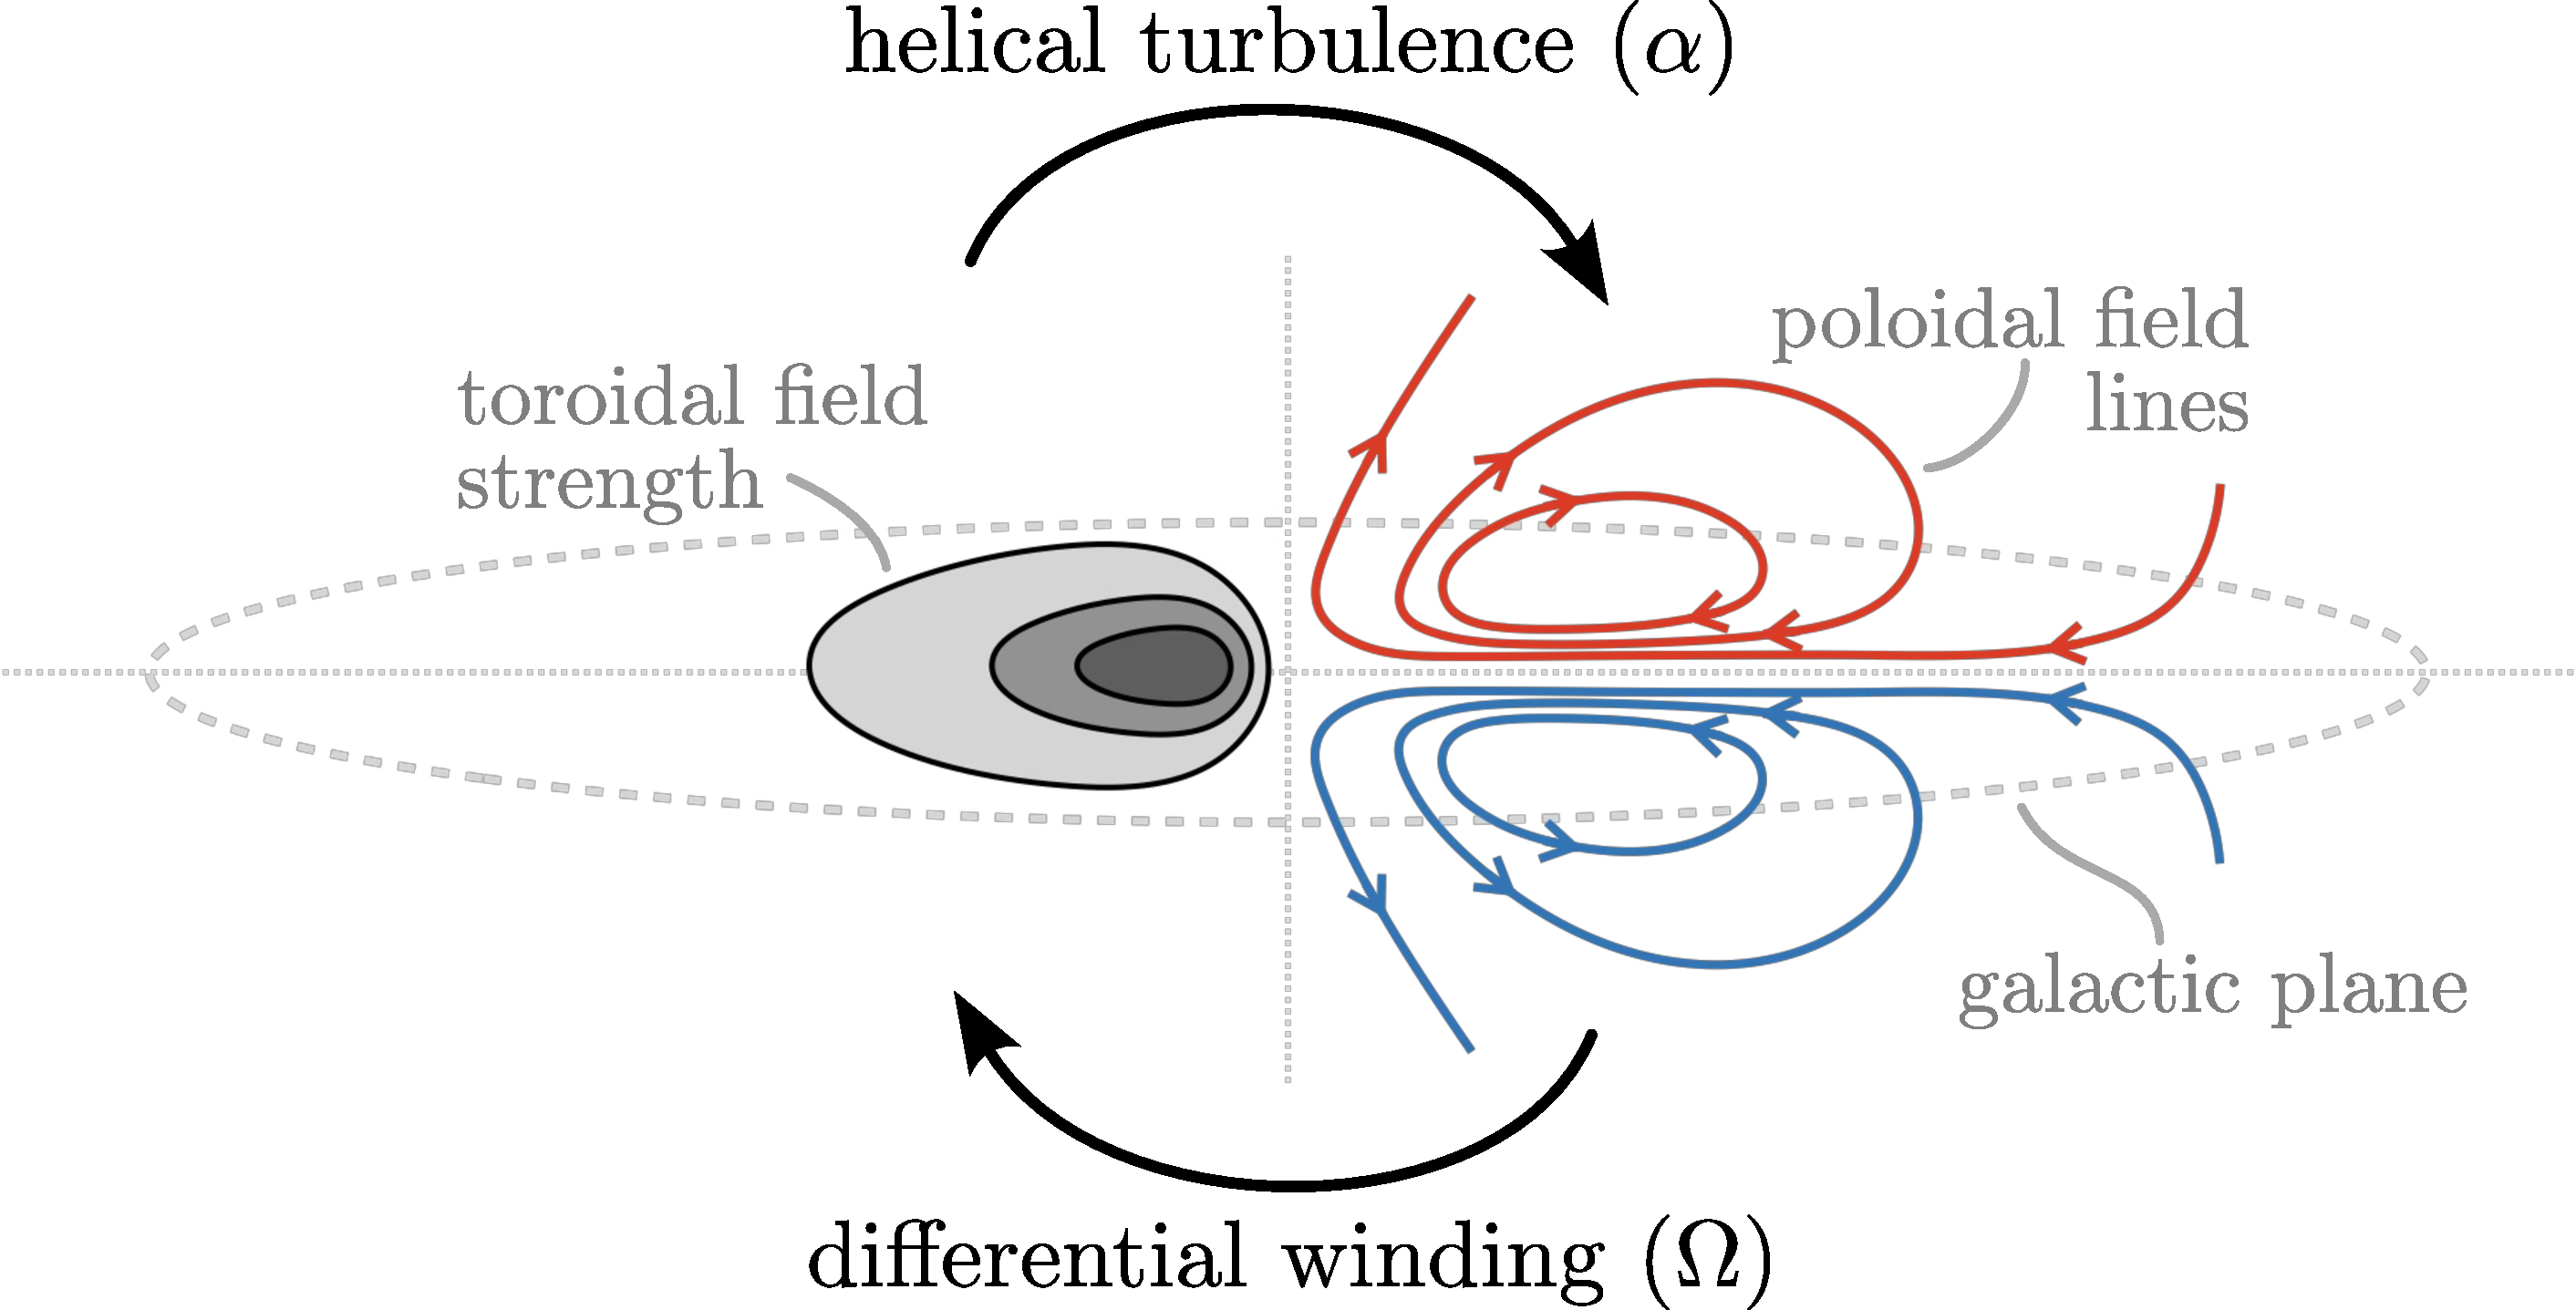
\includegraphics[width=0.9\linewidth]{figures/introduction/galaxy.pdf}
    \caption{Schematic of an $\alpha-\Omega$ dynamo operating in a galaxy, adapted from \citet{klein2014galactic}. The large-scale galactic magnetic field is decomposed into a toroidal component (left; wrapped around the disc's rotation axis) and a poloidal component (right; field lines thread the disc and halo). Differential rotation winds poloidal flux into toroidal flux (the $\Omega$ effect), and helical turbulence regenerates poloidal fields from toroidal ones (the $\alpha$ effect). Together, these two processes create a closed feedback loop that can generate and maintain coherent large-scale structure against turbulent and resistive diffusion.}
    \label{fig:galaxy}
\end{figure}

In large spiral galaxies, where differential rotation is both strong and coherent on $\sim \mathrm{kpc}$ scales, it is easy for this condition to be satisfied. For example, \citet{ntormousi2020dynamo} used direct numerical simulations to show that an $\alpha$-$\Omega$ LSD was active in a Milky Way-like galaxy, where an ordered field was measured to grow over $\sim 0.5 \,\mathrm{Gyr}$. This growth is consistent with our estimate for $\gamma$ above, which, for a typical spiral-galaxy, where $L \sim 10 \,\mathrm{kpc}$, $\alpha \sim 1 \,\mathrm{km} \,\mathrm{s}^{-1}$, and $r |\mdd \Omega / \mdd r| \sim \Omega \sim 30 \,\mathrm{km} \,\mathrm{s}^{-1} \,\mathrm{kpc}^{-1}$, gives $\gamma \approx 2\times 10^{-3} \,\mathrm{Myr}^{-1}$. As we discuss in the next section, this rate of amplification is notably slower than small-scale dynamo growth, which is driven by the same turbulent motions. The LSD is therefore unlikely to be the sole (or primary) mechanism for galactic magnetic field strengths, even in large spiral galaxies. The role of the LSD is even more questionable in smaller galaxies, where differential rotation is weaker and often less coherent. In these systems, the $\Omega$-effect becomes inefficient, and diffusion can more easily overwhelm large-scale growth, so an $\alpha$-$\Omega$ LSD struggles to explain the inferred field amplitudes. Nonetheless, the LSD provides a natural route to generating the coherent large-scale structure observed in spiral discs.

% Parker (1955) phenomenology [Rincon 4.2.2]. Steenbeck, Krause \& Radler (1966), Vainshtein (1970), Moffatt (1970) [Rincon 4.3].

\subsubsection{Small Scale Dynamos}
\label{sec:evolve:ssd}

A key element of the $\alpha$-$\Omega$ dynamo is the role played by velocity fluctuations, $\delta\mVector{u}$. While they contribute an important ingredient for amplifying large-scale magnetic fields via their role in the net correlation $\overline{\delta\mVector{u}\times\delta\mVector{b}}$ in \autoref{eqn:lsd:average}, they can also drive local magnetic amplification on the scales of the fluctuations themselves. Here we will focus on these fluctuations, and show that they produce the fastest, most efficient, and readily \DIFaddbegin \DIFadd{available }\DIFaddend scenario for magnetic amplification.

Working in a locally comoving frame where $\bar{\mVector{u}} \approx \mVector{0}$, we will, for notational convenience, write $\mVector{u} \equiv \delta\mVector{u}$ and $\mVector{b} \equiv \delta\mVector{b}$, and drop the $\delta$ symbol. Local amplification  then follows from the interactions of fluctuating velocity gradients with the magnetic field, where only certain interactions are productive. To see which motions grow the magnetic energy density, consider
\begin{align}
    \mDDFrac{\psi_\mathrm{mag}}{t}
        = \frac{1}{4\pi} \rbrac{
                \overbrace{
                    \mVector{b}\otimes\mVector{b}:\nabla\otimes\mVector{u}
                }^\text{\shortstack{stretching\\ + compression}}
                - \underbrace{
                    b^2 \rbrac{\nabla\cdot\mVector{u}}
                }_\text{compression}
                - \overbrace{
                    \eta \,\mVector{b}\cdot\nabla^2\mVector{b}
                }^\text{diffusion}
            }
        \label{eqn:induction:lagrangian}
    .
\end{align}

Using index notation for the moment, the first term $ b_i b_j \mpp_j u_i $ measures the component of the velocity gradient projected along the local field direction, which contains both strain and compressive contributions. Following \citet{beattie2023bulk}, it is useful to decompose the velocity gradient tensor into $\mpp_j u_i = S_{ij} + R_{ij} + C_{ij}$, where
\begin{align}
    S_{ij}
        &\equiv \frac{1}{2} \rbrac{\mpp_j u_i + \mpp_i u_j}
            - \frac{1}{3} (\mpp_k u_k) \delta_{ij}
        & \mbox{(strain)} \\
    R_{ij}
        &\equiv \frac{1}{2} \rbrac{\mpp_j u_i - \mpp_i u_j}
        & \mbox{(rotation)} \\
    C_{ij}
        &\equiv \frac{1}{3} (\mpp_k u_k) \delta_{ij}
        . & \mbox{(compression)}
\end{align}
This split reveals the three fundamental types of local actions that a flow can perform on a fluid element, namely, volume-preserving deformation $\mTensor{S}$, rigid rotation $\mTensor{R}$, and isotropic volume change $\mTensor{C}$ (with compression or expansion set by the sign of $\theta \equiv \mathrm{Tr}(\mTensor{C})$), respectively.

The first model to demonstrate how fluctuating velocity fields can drive magnetic amplification was put forward by \citet{moffatt1961amplification} for incompressible flows ($\theta = 0$), and later extended by \citet{zel1984kinematic} to flows with finite correlation times. It is popularly referred to as the \textit{stretch-twist-fold} mechanism, and is best viewed as a pedagogical picture that explains how magnetic amplification is possible through a small set of repeatable, local deformations acting on a magnetic flux tube. In the language of \citet{beattie2023bulk} (see also \citealt{schekochihin2002spectra, seta2021saturation, sur2024role}\DIFdelbegin \DIFdel{; see, however, Footnote~4 in \mbox{%DIFAUXCMD
\citealt{beattie2023bulk}}\hskip0pt%DIFAUXCMD
}\DIFdelend ), these actions map naturally onto the strain and rotation tensors, $\mTensor{S}$ and $\mTensor{R}$, together with diffusion.

\begin{figure}
    \centering
    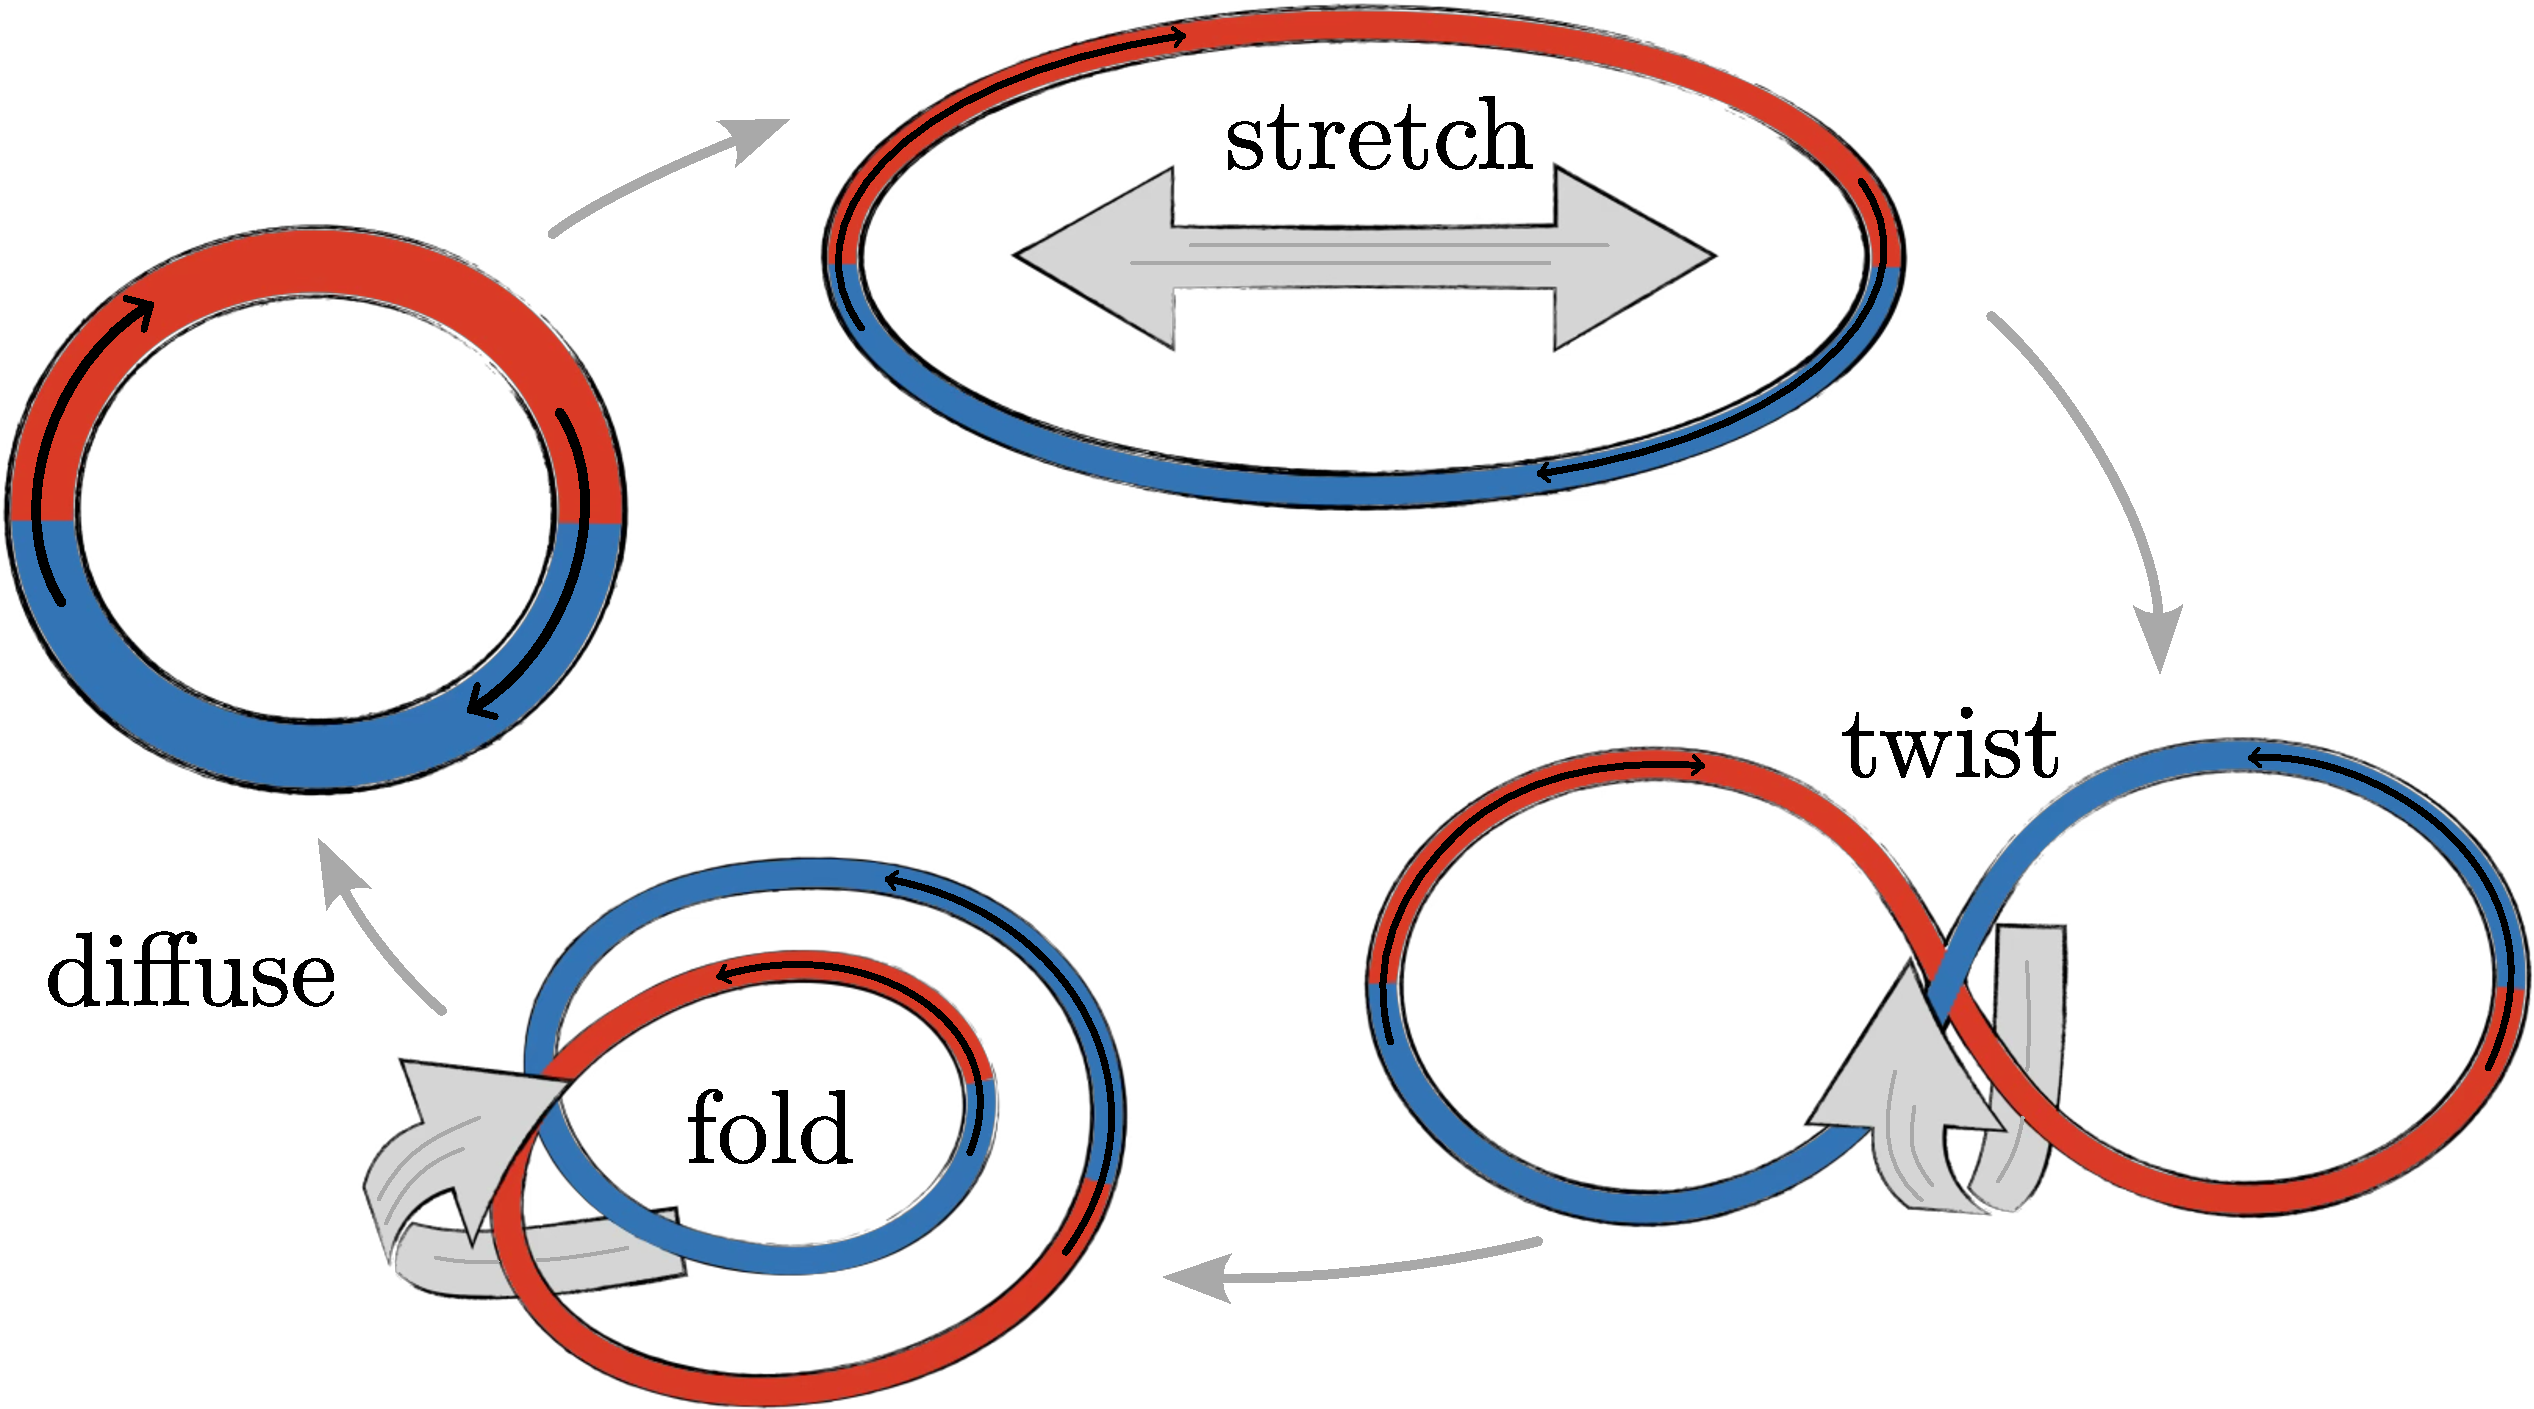
\includegraphics[width=0.8\linewidth]{figures/introduction/STF.pdf}
    \caption{Schematic of the \textit{stretch-twist-fold} (and diffuse) mechanism, adapted from \citet{rincon2019dynamo}. A closed loop of magnetic field is repeatedly (i) stretched by strain, concentrating flux into a smaller cross-section, thereby increasing magnetic energy; (ii) twisted and reoriented by rotational motions; and (iii) folded to bring segments of opposite polarity into close contact; (iv) diffusion merges the folded segments, making this cycle irreversible.}
    \label{fig:STF}
\end{figure}

Stretching is induced when strain acts along the local field direction, $\mVector{b}\otimes\mVector{b}:\mTensor{S}$, which concentrates magnetic flux into progressively thinner cross-sections and thereby increases the local magnetic energy density. Sustained growth then requires repeated stretching events, but repeated, random deformation events need not lead to monotonic amplification, since the evolution remains reversible: random stretching events may counter one-another. Rotation, while unable to change the magnetic energy density directly\footnote{
    Since $b_i b_j$ is symmetric and $R_{ij}$ is antisymmetric, $b_i b_j R_{ij} = 0$, which matches the intuition that pure rotation can reorient $\mVector{b}$ but cannot change its magnitude.
}, plays an important role by reorienting the field loop, which can lead to twisting and folding of the field. Diffusion then provides the final, essential ingredient for making this process irreversible\footnote{
    This should really be called the \textit{stretch-twist-fold-diffuse} mechanism.
}, merging the field after it has been stretched, twisted, and folded. This is summarised in \autoref{fig:STF}.

In real plasma flows, this picture should not be interpreted as a literal, coherent sequence of actions acting on a single magnetic flux tube, but instead as a statistical description of what happens to bundles of magnetic field lines as they are entrained in stochastic, often turbulent flows. \citet{kazantsev1968} successfully turned this statistical idea into a quantitative theory by deriving an evolution equation whose growing solution predicts a magnetic energy spectrum (see \citealt{rincon2019dynamo} for details) with asymptotic form
\begin{align}
    \psi_\mathrm{mag}(k, t)
        \propto \exp(\gamma t) \rfrac{k}{k_\eta}^{3/2} K_0\rfrac{k}{k_\eta}
        ,
        \label{eqn:kazantsev}
\end{align}
where $K_0$ is a Macdonald function, $k \equiv 2\pi / \ell$ is the Fourier wavenumber, $k_\eta$ is the resistive wavenumber (where $\mRem \sim 1$), and $\gamma \sim \mAve{\mVectorUnit{b}\otimes\mVectorUnit{b}:\mTensor{S}}_{\mSurface(t)}$ is the average rate of field-line stretching along advected material surfaces $\mSurface(t)$.

Although it was originally formulated for solar magnetic fields, \autoref{eqn:kazantsev} has since proven remarkably successful at predicting magnetic field statistics in turbulent systems, and, since turbulence is ubiquitous\footnote{
    The ``big power-law in the sky'' suggests turbulent velocity fluctuations span across more than six decades: from $\sim 10^4\,\mathrm{pc}$ down to $\lesssim 10^{-2}\,\mathrm{pc}$; see, \eg \citet{kalberla2019turbulent} and \citet{liu2025tiny}.
}, in astrophysical plasmas, the theory has found widespread success, including in \DIFdelbegin \DIFdel{the interstellar medium}\DIFdelend \DIFaddbegin \DIFadd{supernova-driven, multiphase ISM simulations \mbox{%DIFAUXCMD
\citep{gent2023transition}}\hskip0pt%DIFAUXCMD
}\DIFaddend . \citet{kulsrud1992spectrum} and \citet{schekochihin2001structure}, for example, coupled the Kazantsev \DIFaddbegin \DIFadd{\mbox{%DIFAUXCMD
\citep{kazantsev1968} }\hskip0pt%DIFAUXCMD
}\DIFaddend framework to Kolmogorov turbulence, which led to a picture of magnetic growth where stretching becomes controlled by the fastest, and thus smallest, turbulent eddies, $\ell_\nu$ (where $\mReh \sim 1$; confirmed in, \eg \citealt{kriel2022fundamental}). This leads to growth rate $\gamma \sim 1 / t_\nu \sim u_\nu/\ell_\nu \sim (u_0 / \ell_0) \,\mReh^{1/2}$, which, in the $\mReh \gg 1$ interstellar medium predicts SSD growth on dynamical timescales $\sim \mathrm{Myr}$, which is significantly faster than the $\alpha$-$\Omega$ LSD \citep[\eg][]{gent2023transition}\DIFaddbegin \DIFadd{, though LSD efficiency can be limited by $\alpha$-quenching \mbox{%DIFAUXCMD
\citep{vishniac2001magnetic}}\hskip0pt%DIFAUXCMD
}\DIFaddend .

The current paradigm for galactic magnetism is therefore that SSD action is essentially inevitable, and provides the most efficient route for magnetic amplification. Given its ingredients are readily available across all epochs of galaxy evolution, it believed that SSDs ultimately set the overall magnetic field strength. In galaxies that can also support an LSD, for example the $\alpha$-$\Omega$ dynamo we discussed in \S\ref{sec:evolve:lsd}, large-scale induction then acts on already amplified magnetic fields to organise them into coherent, ordered fields. This coherence is not permanent, however, since mergers can disrupt disc rotation and reintroduce strong turbulence, effectively resetting the large-scale ordering and returning the magnetic system to an SSD-dominated state until coherent rotation re-emerges.


\section{Thesis Roadmap and Remaining Lacunae}
\label{sec:intro:roadmap}

The remainder of this thesis is organised around three paper-chapters. The first two chapters are published papers, and explore aspects of SSD amplification with particular emphasis on the role of compressibility. The final chapter is a code-development paper in the final stages of preparation, wherein we implement \DIFdelbegin \DIFdel{ideal MHD }\DIFdelend \DIFaddbegin \DIFadd{an MHD module }\DIFaddend in a new astrophysical simulation code. Below we briefly motivate each chapter; each chapter also includes a dedicated introduction that provides further context and an overview of the relevant literature.

\uline{\S\ref{chapter:ssd-exp} focuses on kinematic SSD amplification in compressible turbulence.} While the classical Kazantsev formalism provides a quantitative description of kinematic dynamo growth, it is most often (as discussed in \S\ref{sec:evolve:ssd}) interpreted through the lens of incompressible turbulence models. Extensions beyond the incompressible limit have been developed for compressible flows \citep[\eg][]{schober2012magnetic, bovino2013turbulent}, but their consequences for the generated magnetic structures remain comparatively less explored. This matters because compressibility introduces shocks and strong density intermittency that affect how SSDs operate \citep{federrath2016magnetic}. Because shocks potentially organise magnetic fields on large scales, compressibility may help explain the $\sim \mathrm{kpc}$-scale magnetic structure inferred in young galaxies (see \S\ref{sec:what-we-see}) at epochs when LSDs are unlikely to have had time to organise coherent fields. \S\ref{chapter:ssd-exp} explores whether compressibility can indeed help resolve this tension.

\uline{\S\ref{chapter:ssd-nl} focuses on the nonlinear stage of SSD amplification}, when magnetic fields become dynamically important and begin to modify the stretching motions that amplify them. It is well understood that SSD growth is exponential in the kinematic stage, but the subsequent nonlinear evolution remains an active area of debate. While many theories make predictions for the growth rate, efficiency, and timescale of saturation, there has been a lack of systematic work to test them. These uncertainties are further exacerbated in compressible turbulence because shocks and strong intermittency introduce additional couplings. Progress has largely been limited by the fact that the nonlinear stage is transient and mediated by intermittent flows, so measurements from any single realisation are strongly stochastic. \S\ref{chapter:ssd-nl} therefore develops a statistical framework based on ensembles of simulations, designed to extract the deterministic behaviour underlying nonlinear SSD growth and to obtain measurements that can directly test proposed nonlinear theories.

Finally, \DIFdelbegin %DIFDELCMD < \uline{\S\ref{chapter:quokka} implements a new ideal-MHD constrained-transport (CT) scheme in the \textsc{Quokka} codebase}%%%
\DIFdelend \DIFaddbegin \uline{\S\ref{chapter:quokka} implements a new MHD constrained-transport (CT) scheme in the \textsc{Quokka} codebase}\DIFaddend . Following the dynamical roads discussed in \S\ref{sec:evolve:paths}, it is clear that a single, self-consistent simulation of galaxy evolution requires resolving a wide dynamic range, from $\sim 10 \,\mathrm{kpc}$ down to $\sim 10 \,\mathrm{pc}$. This has been difficult to achieve with existing CPU-based codes, but is now becoming practical with next-generation, GPU-accelerated supercomputers, which \textsc{Quokka} was developed for from its outset. Until now, however, \textsc{Quokka} has lacked an MHD module. In \S\ref{chapter:quokka} we discuss our implementation of a new CT-based scheme, and validate that it  is both accurate enough for these applications, while remaining efficient enough to scale to the required resolutions.

    \chapter{Magnetic Structures in Supersonic Small-Scale Dynamos}
\label{chapter:ssd-exp}

\noindent\hfill\parbox{0.865\textwidth}{\raggedleft
This chapter is mildly adapted from:
\textit{Kriel, N., Beattie, J. R., Federrath, C., Krumholz, M. R., \& Hew, J., 2025, Fundamental MHD scales -- II: the kinematic phase of the supersonic small-scale dynamo, MNRAS, 537(3), 2602–2629, doi:\href{https://doi.org/10.1093/mnras/staf188}{10.1093/mnras/staf188}}
}\par

\section{Chapter Abstract}

Many astrophysical small-scale dynamos (SSDs) amplify weak magnetic fields via highly compressible, supersonic turbulence, but most established SSD theories have only considered incompressible flows. To address this gap, we perform visco-resistive SSD simulations across a range of sonic Mach numbers ($\mathcal{M}$), hydrodynamic Reynolds numbers ($\mReh$), and magnetic Prandtl numbers ($\mPrm$), focusing on the exponential growth phase. From these simulations, we develop robust measurements of the kinetic and magnetic energy dissipation scales ($\ell_\nu$ and $\ell_\eta$, respectively), and show that $\ell_\nu/\ell_\eta \sim \mPrm^{1/2}$ is a universal feature of turbulent ($\mReh \geq \mReh_\mathrm{crit} \approx 100$), $\mPrm \geq 1$ SSDs, regardless of $\mathcal{M}$. We also measure the scale of maximum magnetic field strength ($\ell_\mathrm{p}$), where we confirm that incompressible SSDs (where either $\mathcal{M} \leq 1$ or $\mReh < \mReh_\mathrm{crit}$) concentrate magnetic energy at $\ell_\mathrm{p} \sim \ell_\eta$ with inversely correlated field strength and curvature. By contrast, for compressible SSDs (where $\mathcal{M} > 1$ and $\mReh \geq \mReh_\mathrm{crit}$), shocks concentrate magnetic energy in large, over-dense, coherent structures with \DIFdelbegin \DIFdel{$\ell_\mathrm{p} \sim (\ell_0 / \ell_\mathrm{shock})^{1/3} \ell_\eta \gg \ell_\eta$}\DIFdelend \DIFaddbegin \DIFadd{$\ell_\mathrm{p} \sim (\ell_\mathrm{turb} / \ell_\mathrm{shock})^{1/3} \ell_\eta \gg \ell_\eta$}\DIFaddend , where $\ell_\mathrm{shock}$ is the characteristic shock width, and \DIFdelbegin \DIFdel{$\ell_0$ }\DIFdelend \DIFaddbegin \DIFadd{$\ell_\mathrm{turb}$ }\DIFaddend is the outer scale of the turbulent field. When $\mPrm < \mReh^{2/3}$, the shift of $\ell_\mathrm{p}$ (from the incompressible to compressible flow regime) is large enough to move the peak magnetic energy scale out of the subviscous range, and the plasma converges on a hierarchy of scales: \DIFdelbegin \DIFdel{$\ell_0 > \ell_\mathrm{p} > \ell_\mathrm{shock} > \ell_\nu > \ell_\eta$}\DIFdelend \DIFaddbegin \DIFadd{$\ell_\mathrm{turb} > \ell_\mathrm{p} > \ell_\mathrm{shock} > \ell_\nu > \ell_\eta$}\DIFaddend . In the compressible flow regime, more broadly, we also find that magnetic field-line curvature becomes nearly independent of the field strength, not because the field geometry has changed, but instead the field becomes locally amplified through flux-frozen compression by shocks. These results have implications for various astrophysical plasma environments in the early Universe, and cosmic ray transport models in the interstellar medium.

\section{Chapter Introduction}

\subsection{Setting the Stage for Present-Day Galactic Magnetism}

As far as we understand, the Universe was born without magnetic fields. This, however, stands in stark contrast with the present-day Universe, where dynamically important magnetic fields are observed to be ubiquitous \citep[see][for recent reviews on magnetic fields in galaxies and their impact on star formation]{krumholz2019role, brandenburg2023galactic}. While the origin of these fields remains uncertain, two main candidates exist: phase transitions during inflation, which could have generated fields with strengths ranging from $10^{-36}$ to $10^{-8} \,\mathrm{G}$, varying on $\sim \mathrm{Mpc}$ scales \citep{quashnock1989magnetic, sigl1997primordial, kahniashvili2013evolution}, and battery processes during the epoch of re-ionisation ($z \sim 35$--$6$) \citep{biermann1950ursprung, naoz2013generation}, which could have produced fields of around $10^{-24} \,\mathrm{G}$ on $\sim 10 \,\mathrm{kpc}$ scales.

Regardless of which mechanism seeded the first magnetic fields, primordial fields are believed to have decayed until the structure formation era at $z \sim 2$ \citep[\eg][]{brandenburg2017evolution, vachaspati2021progress, hosking2022cosmic, mtchedlidze2022evolution, mtchedlidze2023inflationary, Hosking2023_cosmic_voids_nature}, by which time they would have been more than $15$ orders of magnitude weaker than the $\sim \mu\mathrm{G}$ fields observed on $\sim \mathrm{kpc}$ scales in the Milky Way and in other nearby galaxies \citep[\eg][]{kulsrud1997protogalactic, beck2019synthesizing, shah2021magnetic, lopez2022extragalactic}. Present-day magnetic fields, therefore, cannot simply be relics from electroweak phase transitions or battery processes in the early Universe, and instead some mechanism must have amplified them dramatically.

\subsection{Flavours of Dynamo}

Dynamo action is believed to be the most plausible mechanism for amplifying primordially-produced fields to the levels we observe in the present-day \citep[\eg][]{latif2013small, mtchedlidze2022evolution, mtchedlidze2023inflationary}, and broadly describes the process by which initially weak magnetic fields are amplified and subsequently maintained through the conversion of kinetic into magnetic energy (see \citealt{rincon2019dynamo, brandenburg2023galactic} for recent reviews, and \citealt{tzeferacos2018laboratory, bott2021time, bott2022insensitivity} for recent laboratory experiments). These mechanisms are categorised either as small-scale dynamos (SSDs) or large-scale dynamos (LSDs), determined by the scale on which magnetic fields are grown relative to the fields that amplify them. In the current paradigm for the origin of galactic magnetic fields, both SSDs and LSDs are believed to be important, but are understood to play very different roles \citep[see, \eg][for recent works]{bhat2016unified, pakmor2017magnetic, rieder2017dynamo2, rieder2017dynamo3, steinwandel2023towards, gent2023transition}.

\subsubsection{Small-Scale Dynamos}

SSDs in the interstellar medium (ISM) of galaxies are primarily driven by supersonic turbulence, in turn supported by a combination of supernova feedback and gravitational instabilities \citep{krumholz2016turbulence, bacchini2020evidence}. Starting with initially weak (primordial) seed fields, these SSDs follow roughly a three-stage process: (1) random kinetic motions (or more precisely, random velocity gradients) \citep[\eg][]{vainshtein1972origin, zel1984kinematic, archontis2003numerical} amplify magnetic energy exponentially fast-in-time (termed the kinematic phase); (2), once magnetic fields are strong enough to impart a backreaction on the flow via the Lorentz force, growth slows down to polynomial-in-time \citep[termed the nonlinear phase; \eg][see also \S\ref{sec:discussion:saturation} for a discussion]{schekochihin2004simulations, beresnyak2012universal, Schleicher2013_quadratic_growth, Xu2016_dynamo, seta2020seed}; finally (3), once the magnetic field is in close equipartition with kinetic energy, the field strength saturates and continues to be maintained at this level via the velocity field \citep[\eg][]{schekochihin2002spectra, cho2009growth, seta2021saturation, beattie2022growth}.

\subsubsection{Large-Scale Dynamos}

Galactic LSDs are also capable of exponential magnetic growth over $\sim \mathrm{Gyr}$ timescales, which could be driven by a mix of helical turbulence \citep[\eg][]{bhat2016unified, rincon2021helical}, potentially due in part to galactic differential rotation/shear \citep[\eg][]{vishniac1997incoherent, kapyla2008large, squire2015generation, gent2023transition}, or magnetic instabilities \citep[\eg][]{johansen2008high, qazi2023nonlinear}. While catastrophic quenching at high magnetic resistivity has been a concern, particularly in domains with either closed or periodic boundaries, where magnetic helicity cannot escape \citep[see][]{vishniac2001magnetic}, this effect is believed to be less severe than previously thought, especially in shearing systems \citep{hubbard2012catastrophic}. Moreover, quenching can be alleviated by factors like non-conservation of helicity flux \citep{verma2003energy, sur2007galactic, del2013turbulent}, as would be the case in the presence of outflows (\eg galactic winds) and accreting flows, or with the additional influence of cosmic ray pressure \citep{parker1992fast, hanasz2004amplification}. Nonetheless, LSDs alone are not believed to be solely responsible for amplifying primordial fields to the magnitudes we observe today, as they operate much slower than the kinematic phase of SSDs \citep{schober2012magnetic, gent2023transition} and are less efficient in the presence of low resistivity SSDs \cite[\eg][]{gent2023transition}. However, some LSDs, like the shear-current dynamo \citep{squire2015generation}, can directly feed on the turbulent magnetic fluctuations produced by SSDs \citep[see][for a recent, thorough review of LSDs]{brandenburg2023galactic}.

\subsubsection{Dynamos in Young Galaxies}

Supernova-driven SSDs operating in the ISM of young, isolated Milky Way-like galaxies, have been numerically shown to be capable of amplifying primordial magnetic fields with an e-folding time of $\sim 100\,\mathrm{Myr}$, reaching a saturated field strength of $10$--$50 \,\mu\mathrm{G}$ (corresponding to $\sim 10\%$ of equipartition with the kinetic energy) by $z \sim 3$--$2$ \citep{pakmor2017magnetic, rieder2016dynamo1, rieder2017dynamo2, steinwandel2023towards, Muni2024_seed_field_to_dynamo}. As these galaxies evolve and become more quiescent, some yet unconstrained combination of the aforementioned galactic mechanisms creates a LSD that operates on the SSD-amplified fields, gradually contributing to the total magnetic field amplitude and efficiently developing large-scale, ordered fields observed in present-day galaxies \citep{rieder2017dynamo2, gent2023transition, brandenburg2023galactic}. This was demonstrated by \citet{gent2023transition}, where a rotation-driven LSDs was shown to be capable of amplifying the saturated SSD energy state by a factor $\lesssim 10$, over several $\mathrm{Gyr}$, and in doing so, efficiently reorganise SSD amplified magnetic fields to produce large-scale, coherent structures on scales larger than where the SSD operates.

Galaxy mergers are a example of systems where both a SSD and LSD operates in concert \citep{berlok2019impact, pfrommer2022simulating}. While the exact interaction between these two dynamo processes largely remains an open problem, the interplay between the nonlinear phase of the SSD and the LSD is important for re-establishing large-scale order after temporary merger-induced disruption, and for redistributing kinematic SSD-amplified fields from the inner regions, outward \citep{whittingham2021impact, whittingham2023impact}. Nonetheless, for most of this \DIFdelbegin \DIFdel{paper}\DIFdelend \DIFaddbegin \DIFadd{chapter}\DIFaddend , we focus on the kinematic phase, returning briefly to the nonlinear phase in \S\ref{sec:discussion:saturation}.

\subsection{\DIFdelbegin \DIFdel{The Question: }\DIFdelend Does The Small-Scale Dynamo Always Produce Small-Scale Magnetic Fields?}

Our current paradigm for magnetogenesis has recently been challenged by the detection of \mbox{$\lesssim 500 \,\mu\mathrm{G}$} magnetic fields ordered on $5 \,\mathrm{kpc}$ scales in a distant ($z \sim 2.6$) gravitationally micro-lensed galaxy \texttt{9io9} \citep{geach2023polarized}, as well as $\sim \mathrm{kpc}$ fields in a $z \sim 5.6$ galaxy \citep{chen2024kiloparsec}. While the field strength of \texttt{9io9} remains poorly constrained\footnote{
    \citet{geach2023polarized} arrive at an upper bound for the magnetic field strength based on the assumption of energy equipartition between magnetic and kinetic energy. However, even the most efficient dynamos do not reach perfect equipartition on all scales \citep[\eg][]{federrath2011mach, federrath2014turbulent, kriel2022fundamental, beattie2022growth}. For supersonic dynamos, which are expected to be important in the cold molecular gas traced in \texttt{9io9}, the final saturation is more likely $\sim 1\%$, which means \texttt{9io9} is more likely in a $\sim \,\mu\mathrm{G}$ state, making it consistent with the field strengths of modern galaxies.
}, the fact that it is ordered on $\sim \mathrm{kpc}$ scales poses a problem for the model outlined above, since a LSD would not have had enough time to become established\footnote{
    \citet{geach2023polarized} estimate that the dynamo number for \texttt{9io9} is $\approx 3$, which is lower than the critical value $\approx 7$ which is required for a LSD to be estimated as dynamically important in Milky Way-like disc galaxies \citep{ruzmaikin1988magnetism}.
} at $z \sim 2.6$. Moreover, SSDs have been traditionally thought to produce fields that are chaotic on large scales, only becoming ordered on the smallest scales allowed by magnetic dissipation \citep[\eg][]{schekochihin2004simulations, kriel2022fundamental, brandenburg2023dissipative}, which are expected to be $\ll \mathrm{pc}$ in size for ISM conditions \citep{marchand2016chemical}. A similar problem exists in galaxy mergers, where the rapid growth of magnetic energy seen in simulations points to SSD action, but the fields are correlated on $\sim \mathrm{kpc}$ scales, which have been thought to be too large scale to be generated during the kinematic SSD phase \citep[\eg][]{rodenbeck2016magnetic, basu2017detection, brzycki2019parameter, whittingham2021impact}.

Now, the expectation that SSDs only produce small-scale fields, stems from extensive explorations of SSDs in incompressible (\eg subsonic) flow regimes \citep[see seminal works by, \eg][]{kazantsev1968, vainshtein1982theory, vincenzi2002kraichnan, schekochihin2004simulations, boldyrev2004magnetic}. This expectation was confirmed in Paper I of this series \citep[][herein \citetalias{kriel2022fundamental}]{kriel2022fundamental}, where we used direct numerical simulations (DNSs) to explore the magnetic fields produced during the kinematic phase, and showed that the bulk of magnetic energy becomes concentrated at the smallest possible scales in the incompressible problem, \ie the scale where magnetic fields dissipate. Given that these scales are much smaller than a galactic scale height, and fall within the regime where turbulence becomes independent of the anisotropy imposed by the galactic potential \citep{Kortgen2021_power_spectrum_of_isolated_galaxies}, the presence of large-scale shear, differential rotation or other similar organised galactic flows, does not alter this conclusion. However, this understanding may not fully capture the dynamics of more compressible environments.

Both the first galaxies \citep{maio2011impact, mandelker2020instability} and later galaxy mergers \citep{geng2012magnetic, sparre2022gas}, are expected to host highly compressible (\ie supersonic) turbulence. This is because the great majority of their mass, and a substantial fraction of their volume, consists of dense, atomic and molecular gas \citep{cox2006kinematic, krumholz2009star, popping2014evolution, nandakumar2023large} where rapid cooling keeps the sound speed well below the characteristic flow velocity \citep{rees1977cooling, white1978core, birnboim2003virial, Krumholz2020_cr_transport_starburst, li2020impact}. While it has been shown that supersonic flow decreases the efficiency of SSDs \citep{federrath2011mach, federrath2014turbulent, seta2021saturation, seta2022turbulent, hew2023lagrangian}, there has to date been no systematic study of how compressibility changes magnetic field geometry, characteristic turbulence and dynamo scales, or structure of the magnetic field. Given the discrepancy between the observations and the predictions of incompressible SSD models, there is a clear need for such a study. Our goal in this \DIFdelbegin \DIFdel{paper }\DIFdelend \DIFaddbegin \DIFadd{chapter }\DIFaddend is to carefully explore how magnetic fields become organised during the kinematic phase of SSDs driven by supersonic turbulence, and in turn to explore its implications for galaxy mergers and other phenomena that depend on magnetic field structure, most notably new cosmic ray transport models relying on curvature and gyro-radii resonances \citep[\eg][]{kempski2023cosmic, Lemoine2023_field_reversal_CR_transport}.

\subsection{Structure of this Chapter}

The remainder of this \DIFdelbegin \DIFdel{paper }\DIFdelend \DIFaddbegin \DIFadd{chapter }\DIFaddend is structured as follows. In \S\ref{sec:numerics} we describe the numerical simulation suite we use to develop our theoretical model for compressible SSDs. In \S\ref{sec:results} we present and interpret the simulation results, and in \S\ref{sec:discussion} we discuss the implications of these results for a variety of astrophysical systems. We summarise our results and conclusions in \S\ref{sec:conclusion}.

\section{Simulating Small-Scale Dynamos}
\label{sec:numerics}

In this \DIFdelbegin \DIFdel{study }\DIFdelend \DIFaddbegin \DIFadd{chapter }\DIFaddend we use DNSs to explore the kinematic phase of SSDs in plasma flows ranging from viscous to turbulent, and subsonic to supersonic. In \S\ref{sec:mhd_model} we introduce the basic equations that we solve, the numerical method by which we do so, and the initial conditions for our simulations. In \S\ref{sec:ICs} we introduce the key dimensionless parameters that describe different plasma flow regimes, and how we vary these parameters to explore different flow properties. In \S\ref{sec:ICs:nres}, we then discuss issues of convergence.

\subsection{Numerical Approach}
\label{sec:mhd_model}

\subsubsection{Solving the MHD Equations}

For all the simulations in this \DIFdelbegin \DIFdel{study}\DIFdelend \DIFaddbegin \DIFadd{chapter}\DIFaddend , we solve the compressible set of non-ideal (visco-resistive) magnetohydrodynamical (MHD) fluid equations, which in conservative form are
\DIFdelbegin %DIFDELCMD < \begin{align}
%DIFDELCMD <     \mppFrac{\rho}{t}
%DIFDELCMD <         + \nabla\cdot(\rho \mVector{u})
%DIFDELCMD <         &= 0
%DIFDELCMD <         , \label{mhd:continuity} \\
%DIFDELCMD <     \mppFrac{\rho\mVector{u}}{t}
%DIFDELCMD <         + \nabla\cdot\bigg[
%DIFDELCMD <             \rho\mVector{u}\otimes\mVector{u}
%DIFDELCMD <             - \frac{1}{4\pi}\mVector{b}\otimes\mVector{b}
%DIFDELCMD <             \nquad[7]\nonumber \\
%DIFDELCMD <             + \rbrac{c_\mathrm{s}^2\rho + \frac{b^2}{8\pi}}\mTensor{I}
%DIFDELCMD <             - 2\nu\rho\mTensor{V}
%DIFDELCMD <         \bigg] &= \rho\mVector{f}
%DIFDELCMD <         , \label{mhd:momentum} \\
%DIFDELCMD <     \mppFrac{\mVector{b}}{t}
%DIFDELCMD <         - \nabla\times\rbrac{\mVector{u}\times\mVector{b} - \eta\mVector{j}}
%DIFDELCMD <         &= 0
%DIFDELCMD <         , \label{mhd:induction} \\
%DIFDELCMD <     \nabla\cdot\mVector{b}
%DIFDELCMD <         &= 0
%DIFDELCMD <         , \label{mhd:divb_free}
%DIFDELCMD < \end{align}%%%
\DIFdelend \DIFaddbegin \begin{align}
    \mppFrac{\rho}{t}
        + \nabla\cdot(\rho \mVector{u})
        &= 0
        , \label{mhd:continuity} \\
    \mppFrac{\rho\mVector{u}}{t}
        + \nabla\cdot\bigg[
            \rho\mVector{u}\otimes\mVector{u}
            - \frac{1}{4\pi}\mVector{b}\otimes\mVector{b}
            + \rbrac{c_\mathrm{s}^2\rho + \frac{b^2}{8\pi}}\mTensor{I}
            - 2\nu\rho\mTensor{V}
        \bigg] &= \rho\mVector{f}
        , \label{mhd:momentum} \\
    \mppFrac{\mVector{b}}{t}
        - \nabla\times\rbrac{\mVector{u}\times\mVector{b} - \eta\mVector{j}}
        &= 0
        , \label{mhd:induction} \\
    \nabla\cdot\mVector{b}
        &= 0
        , \label{mhd:divb_free}
\end{align}\DIFaddend
for an isothermal plasma evolving over a uniformly discretised, cubic-domain $\ell_{(x, y, z)} \in [0, \ell_\mathrm{box}]$, with triply periodic boundary conditions. Here we use constant (in both space and time) kinematic shear viscosity and Ohmic resistivity, parameterised by the coefficients $\nu$ and $\eta$, respectively, in combination with an external forcing field $\mVector{f}$, to achieve flows with desired plasma numbers (see \S\ref{sec:ICs} for details). The remaining quantities in the equations are the gas density $\rho$, the gas velocity $\mVector{u}$, the sound speed $c_\mathrm{s}$, the current density $\mVector{j} = \nabla\times\mVector{b} /(4\pi)$, and the magnetic field $\mVector{b} = \mVector{b}_0 + \mVector{\delta b}$, which has mean field $\mVector{b}_0$, and fluctuating (turbulent) field $\mVector{\delta b}$ components. Finally, our viscosity model is based on the traceless strain rate tensor, $\mTensor{V}$, where
\begin{align}
    \mTensor{V}
        = \frac{1}{2} \rbrac{
                \nabla\otimes\mVector{u}
                + \rbrac{\nabla\otimes\mVector{u}}^T
            }
            - \frac{1}{3} \rbrac{\nabla\cdot\mVector{u}} \mTensor{I}
        , \label{eqn:strain_rate_tensor}
\end{align}
and $\otimes$ is the tensor product $\nabla\otimes\mVector{u} \equiv \mpp_i u_j$.

We solve \autoref{mhd:continuity}-\ref{mhd:divb_free} with a modified version of the finite-volume \textsc{flash} code \citep{fryxell2000flash, dubey2008introduction}, employing a second-order conservative MUSCL-Hancock 5-wave approximate Riemann solver, described in \citet{bouchut2007multiwave, bouchut2010multiwave}, and implemented into \textsc{flash} by \citet{waagan2011robust}, who showed that it possesses excellent stability properties for highly supersonic MHD flows, with improved efficiency and stability compared with Roe-type solvers. Since our primary interest lies in studying the effects of shocks (a hallmark of supersonic flows), this solver proves highly suitable. Moreover, we utilise the parabolic divergence-cleaning method described by \citet{Marder1987_fluxcleaning} to enforce that $\nabla\cdot\mVector{b} = 0$ modes are diffused away.

\subsubsection{Initial Conditions}

All our simulations use a dimensionless unit system where the simulation box size $\ell_\mathrm{box} = 1$, mean density $\rho_0 = 1$, the sound speed $c_\mathrm{s} = 1$, and magnetic fields are measured in units of $\rho_0^{1/2} c_\mathrm{s} = 1$. We initialise every simulation with uniform density $\rho = \rho_0 = 1$, zero velocity $\mVector{u} = \mVector{0}$, and zero mean magnetic field $\mVector{b}_0 = \mVector{0}$. Since there is no mean magnetic field, and magnetic flux through the simulation volume is conserved, only a fluctuating component can exist, $\mVector{b} = \mVector{\delta b}$. We initialise this fluctuating component with a spectral distribution \citep[using \mbox{\textsc{TurbGen}};][]{Federrath2022_TurbGen} that is non-zero only over the wavenumber range $1 \leq k \ell_\mathrm{box} / 2\pi \leq 3$, with a parabolic profile that peaks at $k \ell_\mathrm{box}/2\pi = 2$, and goes to zero at $k \ell_\mathrm{box}/2\pi = 1$ and $k \ell_\mathrm{box}/2\pi = 3$. Here, the isotropic wavenumber $k$ is defined as per usual: $k \equiv 2\pi / \ell$. We choose the amplitude of this initial parabolic $\mVector{\delta b}$ profile such that the plasma--$\beta \equiv p_\mathrm{th}/p_\mathrm{mag} = 8\pi c_\mathrm{s}^2 \rho_0 / b^2 = 10^{10}$. We note that the exact configuration of the initial seed $\mVector{\delta b}$ field is not important, because it is quickly forgotten by the Markovian-like flow dynamics, and has been shown to not affect the amplification nor the final saturation of the dynamo \citep{seta2020seed, bott2022insensitivity, beattie2022growth}.

\subsection{Important Dimensionless Numbers and Flow Regimes}
\label{sec:ICs}

In this \DIFdelbegin \DIFdel{study }\DIFdelend \DIFaddbegin \DIFadd{chapter }\DIFaddend we explore 34 different simulation configurations, each parameterised by a set of dimensionless numbers that characterise the flow and plasma regimes. Here we introduce each of these numbers, as well as the range of values over which we vary them, before summarising our full set of simulations in \autoref{table:ssd-exp:summary}.

\subsubsection{Sonic Mach Number}
\label{sec:ICs:Mach}

For all our simulations we produce an isotropic, smoothly varying (in time and space) acceleration field via the forcing term, $\mVector{f}$, in \autoref{mhd:momentum}, which is modelled with a generalisation of the Ornstein-Uhlenbeck process in wavenumber-space \citep{eswaran1988examination, schmidt2006numerical, schmidt2009numerical, federrath2010comparing, Federrath2022_TurbGen} using \textsc{TurbGen}. We choose to drive the acceleration field with purely solenoidal modes, \ie $\nabla\cdot\mVector{f} = 0$, because they produce motions that are the most efficient at amplifying magnetic energy \citep{federrath2011mach, federrath2014turbulent, martins2019kazantsev, chirakkara2021efficient}, and tune the amplitude of $\mVector{f}$ in each of our simulations to achieve a root-mean-squared (rms) gas velocity dispersion, $\mAve{u}_\mVolume^{1/2}$, on the driving (outer) scale, \DIFdelbegin \DIFdel{$\ell_0$}\DIFdelend \DIFaddbegin \DIFadd{$\ell_\mathrm{turb}$}\DIFaddend , that lies within $5\%$ of our desired value, \DIFdelbegin \DIFdel{$u_0$}\DIFdelend \DIFaddbegin \DIFadd{$u_\mathrm{turb}$}\DIFaddend ; the notation $\mAve{q}_{\mVolume}$ indicates the volume average of quantity $q$ over the entire simulation domain $\mVolume \equiv \ell_\mathrm{box}^3$. We choose \DIFdelbegin \DIFdel{$\ell_0 = \ell_\mathrm{box}/2$ }\DIFdelend \DIFaddbegin \DIFadd{$\ell_\mathrm{turb} = \ell_\mathrm{box}/2$ }\DIFaddend for all of our simulations to maximise the scale separation between velocity fields and the small-scale magnetic fields they generate, which we achieve by driving $\mVector{f}$ with a parabolic power spectrum that is non-zero only over the wavenumber range $1 \leq k \ell_\mathrm{box}/2\pi \leq 3$, peaking at $k \ell_\mathrm{box} / 2\pi = 2$, and falling to zero at $k \ell_\mathrm{box}/2\pi = 1$ and $k \ell_\mathrm{box}/2\pi = 3$. The corresponding autocorrelation time of $\mVector{f}$, and hence the velocity field, is
\DIFdelbegin %DIFDELCMD < \begin{align}
%DIFDELCMD <     t_0
%DIFDELCMD <         \sim \frac{\ell_0}{u_0}
%DIFDELCMD <         = \frac{2\pi}{k_0 u_0} .
%DIFDELCMD < \end{align}%%%
\DIFdelend \DIFaddbegin \begin{align}
    t_\mathrm{turb}
        \sim \frac{\ell_\mathrm{turb}}{u_\mathrm{turb}}
        = \frac{2\pi}{k_\mathrm{turb} u_\mathrm{turb}} .
\end{align}\DIFaddend

Even though $c_\mathrm{s} = 1$ in our simulations, it is convenient to express the flow velocity relative to the sound speed, \ie the sonic Mach number
\DIFdelbegin %DIFDELCMD < \begin{align}
%DIFDELCMD <     \mSonicMach
%DIFDELCMD <         &\equiv \frac{u_0}{c_\mathrm{s}}
%DIFDELCMD <         . \label{dfn:Mach}
%DIFDELCMD < \end{align}%%%
\DIFdelend \DIFaddbegin \begin{align}
    \mSonicMach
        &\equiv \frac{u_\mathrm{turb}}{c_\mathrm{s}}
        . \label{dfn:Mach}
\end{align}\DIFaddend
We run simulations spanning a wide range of $\mSonicMach$, with $\mSonicMach = 0.3, 1, 5$, and $10$. To get a baseline for how the plasma behaves in the absence of compressible effects, we first run 11 simulations with $\mSonicMach = 0.3$, where \DIFdelbegin \DIFdel{incompressibility in the probability density function (PDF) of $\mSonicMach$ values in }\DIFdelend \DIFaddbegin \DIFadd{the local Mach number fluctuates across }\DIFaddend $\mVolume$ \DIFdelbegin \DIFdel{holds up to $3$-sigma fluctuations}\footnote{\DIFdel{From the density dispersion-Mach relation we expect $\mSonicMach = 0.3$ fields driven by solenoidal forcing to have $\approx 10\%$ fluctuations in the density field \mbox{%DIFAUXCMD
\citep{padoan1997supersonic, passot2003correlation, federrath2008density, federrath2010comparing, price2010density, gerrard2023new}}\hskip0pt%DIFAUXCMD
.
}} %DIFAUXCMD
\addtocounter{footnote}{-1}%DIFAUXCMD
\DIFdelend \DIFaddbegin \DIFadd{with standard deviation $\sigma$ about this mean, such that the $3\sigma$ tail }\DIFaddend (assuming Gaussianity) \DIFaddbegin \DIFadd{approaches $\mSonicMach \sim 1$}\footnote{
    \DIFadd{From the density dispersion-Mach relation we expect $\mSonicMach = 0.3$ fields driven by solenoidal forcing to have $\approx 10\%$ fluctuations in the density field \mbox{%DIFAUXCMD
\citep{padoan1997supersonic, passot2003correlation, federrath2008density, federrath2010comparing, price2010density, gerrard2023new}}\hskip0pt%DIFAUXCMD
.
}}\DIFaddend . This is the regime we previously explored in \citetalias{kriel2022fundamental}, and is relevant for studying \citet{kolmogorov1941dissipation}-like turbulence. In addition to these simulations, we also run a set of four transsonic simulations, $\mSonicMach = 1$, but then turn most of our attention towards the supersonic flow regime, where we run 16 simulations with $\mSonicMach = 5$ and three simulations with $\mSonicMach = 10$. Here, in the highly-compressible ($\mSonicMach \gtrsim 1$) flow regime, one expects to see \citet{burgers1948_turbulence_model}-like turbulence \citep[see for example][]{federrath2013universality, Federrath2021_sonic_scale}.

\subsubsection{Hydrodynamic Reynolds Number}

The second dimensionless parameter that characterises our simulations is the hydrodynamic Reynolds number
\DIFdelbegin %DIFDELCMD < \begin{align}
%DIFDELCMD <     \mReh
%DIFDELCMD <         \equiv \frac{u_0 \,\ell_0}{\nu}
%DIFDELCMD <         \sim \frac{
%DIFDELCMD <                 \|\nabla\cdot(\rho\mVector{u}\otimes\mVector{u})\|
%DIFDELCMD <             }{
%DIFDELCMD <                 \|\nabla\cdot(2\nu\rho\mTensor{V})\|
%DIFDELCMD <             }
%DIFDELCMD <         , \label{dfn:Reyh}
%DIFDELCMD < \end{align}%%%
\DIFdelend \DIFaddbegin \begin{align}
    \mReh
        \equiv \frac{u_\mathrm{turb} \,\ell_\mathrm{turb}}{\nu}
        \sim \frac{
                \|\nabla\cdot(\rho\mVector{u}\otimes\mVector{u})\|
            }{
                \|\nabla\cdot(2\nu\rho\mTensor{V})\|
            }
        , \label{dfn:Reyh}
\end{align}\DIFaddend
which describes the relative importance of inertial compared to viscous forces in a flow; here $\|\dots\|$ is the 2-norm.

In \citetalias{kriel2022fundamental}, we identified $\mReh_\mathrm{crit} \approx 100$ as a critical threshold for $\mReh$ during the kinematic phase, separating viscous ($\mReh < \mReh_\mathrm{crit}$) from turbulent ($\mReh \geq \mReh_\mathrm{crit}$) flows, with several flow properties changing across this boundary. Above this threshold, the flow becomes more turbulent, leading to intermittent velocity fluctuations\footnote{
    Velocity gradients reflect local deformation rates and energy dissipation, where larger, more intermittent gradients indicating turbulence, and conversely, smaller, more uniform gradients suggest viscous flow \citep{schumacher2014small}.
} (super-Gaussian kurtosis), while flows below this value show sub-Gaussian kurtosis. Similarly, the kinetic energy\footnote{
    In turbulence theory, naming conventions originally inspired by \citet{kolmogorov1941dissipation}, primarily apply to incompressible (\mbox{$\mSonicMach \ll 1$}) flows. In these flows, the time-derivative of the average kinetic energy $\mpp_t\big[\mAve{E_\mathrm{kin}}_\mVolume\big] = 0.5\, \mAve{\rho}_\mVolume \mpp_t\sbrac{\mAve{u^2}_\mVolume} \sim \mpp_t\sbrac{\mAve{u^2}_\mVolume}$, assuming that density fields are roughly constant in time, while velocity fields vary in time. However, for highly compressible ($\mSonicMach \gg 1$) flows, these conventions need to be adjusted to account for the time variation in both $\rho$ and $u$, as well as their covariance. As a result, $\ell_\nu$ represents the characteristic dissipation scale of kinetic energy, not just the velocity field.
    \label{note:naming_convesions}
} dissipation (viscous) scale\footnote{
    While $\ell_\nu$ is the characteristic viscous scale, where kinetic fluctuations transition from inertial dominated to viscous dominated, there are in fact a whole range of scales $\ell \lesssim \ell_\nu$ over which dissipation takes place \citep[\eg][]{frisch1991prediction, chen1993far}. These dissipation scales have also been shown to be directly affected by the degree of intermittency of velocity gradient fluctuations \citep[\eg][]{schumacher2007sub}.
} follows the theoretically-expected scaling $\ell_\nu \sim \mReh^{3/4}$ \citep{kolmogorov1941dissipation} for turbulent flows, and then scales as $\ell_\nu \sim \mReh^{3/8}$ for viscous flows \citepalias{kriel2022fundamental}.


Based on this, we explore $10 \leq \mReh < 3000$, where we run most of our simulations with $\mReh \geq \mReh_\mathrm{crit}$ (in the turbulent regime), and dedicate a small portion of our simulations to $10 \leq \mReh < \mReh_\mathrm{crit}$, to explore the transitional regime towards viscous flows.

\subsubsection{Magnetic Prandtl Number}
\label{sec:ICs:Pm}

Our final two dimensionless numbers\footnote{
    Instead of parameterising our flows with respect to the dimensionless Alfv\'enic Mach number ($\mAlfvenMach$), we follow SSD conventions, and use the magnetic-to-kinetic energy ratio ($E_\mathrm{mag} / E_\mathrm{kin}$). In purely fluctuation plasmas, these two quantities are directly related: $\mAlfvenMach = (4\pi \rho)^{1/2} \mAve{u^2}_\mVolume^{1/2} / \mAve{b^2}_\mVolume^{1/2} = (E_\mathrm{mag} / E_\mathrm{kin})^{-1/2}$. Thus, we choose $E_\mathrm{mag} / E_\mathrm{kin}$ as our measure for the significance of Lorentz forces in the flow, where, during the kinematic phase, $E_\mathrm{mag} / E_\mathrm{kin} \ll 1$, meaning $\mAlfvenMach \gg 1$ and Lorentz forces are negligible.
} are the magnetic Reynolds number and the magnetic Prandtl number. The magnetic Reynolds number is defined as
\DIFdelbegin %DIFDELCMD < \begin{align}
%DIFDELCMD <     \mRem
%DIFDELCMD <         \equiv \frac{u_0 \,\ell_0}{\eta}
%DIFDELCMD <         \sim \frac{
%DIFDELCMD <                 \|\nabla\times(\mVector{u}\times\mVector{b})\|
%DIFDELCMD <             }{
%DIFDELCMD <                 \|\eta\nabla\times\mVector{j}\|
%DIFDELCMD <             }
%DIFDELCMD <         , \label{dfn:Reym}
%DIFDELCMD < \end{align}%%%
\DIFdelend \DIFaddbegin \begin{align}
    \mRem
        \equiv \frac{u_\mathrm{turb} \,\ell_\mathrm{turb}}{\eta}
        \sim \frac{
                \|\nabla\times(\mVector{u}\times\mVector{b})\|
            }{
                \|\eta\nabla\times\mVector{j}\|
            }
        , \label{dfn:Reym}
\end{align}\DIFaddend
which, analogously to the hydrodynamic Reynolds number, characterises the relative importance of magnetic induction compared with magnetic (Ohmic) dissipation. The magnetic Prandtl number is then given by
\begin{align}
    \mPrm
        \equiv \frac{\mRem}{\mReh}
        \sim \frac{\nu}{\eta}
        , \label{dfn:Pranm}
\end{align}
and it characterises the relative strength of the magnetic and kinetic energy dissipation. In collisional plasmas, $\mPrm$ is an intrinsic property of the plasma itself, unlike $\mReh$ and $\mRem$, which depend on the flow properties (\ie \DIFdelbegin \DIFdel{$\ell_0$ and $u_0$}\DIFdelend \DIFaddbegin \DIFadd{$\ell_\mathrm{turb}$ and $u_\mathrm{turb}$}\DIFaddend ). In our simulations, we choose values of $1 \leq \mPrm \leq 300$ to explore plasma regimes relevant for most of the gas in the ISM, with a focus on $\mPrm > 1$ scenarios. However, resolution constraints prevent us from exploring turbulent flows with large $\mPrm$. Regardless, in all cases, the characteristic kinetic and magnetic energy ($\ell_\eta$) dissipation scales are organised such that $\ell_\nu \geq \ell_\eta$.

Now, during the kinematic phase of subsonic, $\mPrm > 1$ SSDs, there exist well-established theoretical predictions for the relationships between key MHD length scales: \DIFdelbegin \DIFdel{$\ell_0$}\DIFdelend \DIFaddbegin \DIFadd{$\ell_\mathrm{turb}$}\DIFaddend , $\ell_\nu$, $\ell_\eta$, and the scale $\ell_\mathrm{p}$ where magnetic fields are strongest. \citet{schekochihin2002spectra, schekochihin2004simulations} predicted -- and \citetalias{kriel2022fundamental} and \citet{brandenburg2023dissipative} confirmed numerically -- that magnetic energy becomes strongest on the smallest scales allowed by magnetic dissipation, yielding an ordering of scales $\ell_\mathrm{p} \sim \ell_\eta \sim \ell_\nu \, \mPrm^{-1/2}$. One of the primary goals of our study is to test whether this hierarchy also holds in the supersonic regime.

\subsubsection{Choice of Simulation Parameters}

The discussion of dimensionless numbers above motivates our choice of simulation parameters. To determine the scaling behaviour of $\ell_\eta$ and $\ell_\mathrm{p}$ in compressible flows, we first run a set of eight simulations with $\mRem = 3000$, where we vary $1 \leq \mPrm \leq 300$ while keeping $\mSonicMach = 5$. To isolate the role of compressibility, we then also run a subset of these simulations with $\mSonicMach = 0.3, 1$, and $10$. Next, we run three $\mReh = 500$, $\mSonicMach = 5$ simulations, with $\mPrm = 1, 2$, and $4$, and four $\mReh = 10$, $\mSonicMach = 5$ simulations with $25 \leq \mPrm \leq 250$. Then, to explore the transition from turbulent to viscous flows, we run a set of four $\mSonicMach = 0.3$ simulations, where we fix $\mRem = 500$ and vary $1 \leq \mPrm \leq 50$. Finally, we run two simulations with $\mReh = 2000$ and $\mPrm = 5$ (which gives $\mRem = 10000$), with $\mSonicMach = 0.3$ and $5$, respectively, to confirm that our findings in both the subsonic and supersonic regimes hold in the high-$\mRem$ limit.

We summarise our full set of simulations in \autoref{table:ssd-exp:summary}, adopting a naming convention whereby each simulation is labeled \SimName{\texttt{MMM}}{\texttt{RRR}}{\texttt{PPP}}. Here, \texttt{MMM}, \texttt{RRR}, and \texttt{PPP} give the numerical values of the sonic Mach number, hydrodynamic Reynolds number, and magnetic Prandtl number, respectively. For example, \SimName{5}{600}{5} corresponds with a simulation where $\mSonicMach = 5.0$, $\mReh=600$, and $\mPrm=5$.

\subsection{Numerical Convergence in Time and Resolution}
\label{sec:ICs:nres}

To ensure well-sampled statistics, we run all of our simulations for a duration of \DIFdelbegin \DIFdel{$t = 100 \,t_0$ }\DIFdelend \DIFaddbegin \DIFadd{$t = 100 \,t_\mathrm{turb}$ }\DIFaddend (\ie 100 autocorrelation times of the forcing field), which we show extends well beyond the kinematic phase and into the saturated state of the dynamo for all of our simulations. We also collect data every \DIFdelbegin \DIFdel{$t = 0.1 \,t_0$ }\DIFdelend \DIFaddbegin \DIFadd{$t = 0.1 \,t_\mathrm{turb}$ }\DIFaddend to ensure well-sampled temporal statistics.

To ensure convergence with regard to spatial resolution, we systematically run each of our simulation setups at progressively higher resolution, until our measurements of key characteristic scales: $\ell_\nu$, $\ell_\eta$, and $\ell_\mathrm{p}$ converge. All our simulations use a uniform, cubic grid of $N_\mathrm{res}^3$ cells, where we test for convergence by carrying out simulations at resolutions $N_\mathrm{res} = 18, 36, 72, 144$, and $288$, and then for a subset of our simulations, we also run at higher resolutions of $N_\mathrm{res} = 576$, $1152$ as required (we indicate these simulations in column 13 of \autoref{table:ssd-exp:summary}); we defer a discussion of how we assess convergence to \S\ref{sec:results:nres}.

\begin{table}
\caption{Main simulation parameters and derived quantities.}
\label{table:ssd-exp:summary}

\renewcommand{\arraystretch}{1.05}
\setlength{\tabcolsep}{2.1pt}

\centeronpage{%
\scalebox{0.65}{%
\begin{threeparttable}
\begin{tabular}{l c c c c c c c c c c c c c c}
\hline
\hline
    Sim. ID
    & $\mReh$ & $\mRem$ & $\mPrm$
    & $\mFracSlant{\nu t_0}{\ell_0^2}$ & $\mFracSlant{\eta t_0}{\ell_0^2}$
    & $\mSonicMach$ & $\gamma \, t_0$ & $\rbrac{\frac{E_\mathrm{mag}}{E_\mathrm{kin}}}_\mathrm{sat}$
    & $k_\nu / k_\mathrm{box}$ & $k_\eta / k_\mathrm{box}$ & $k_\mathrm{p} / k_\mathrm{box}$
    & Extra $N_\mathrm{res}$ \\[0.4em]
    \multicolumn{1}{l}{(1)} & (2) & (3) & (4) & (5) & (6) & (7) & (8) & (9) & (10) & (11) & (12) & (13) \\
\hline
\hline
\multicolumn{13}{c}{$\mSonicMach = 0.3$} \\
\hline
$\mSonicMach$0.3Re500Pm1
	& $500$ & $500$ & $1$
	& $3.0 \times 10^{-4}$ & $3.0 \times 10^{-4}$ & $0.30 \pm 0.01$
	& $0.42 \pm 0.01$ & $0.14 \pm 0.03$
	& $23.9 \pm 0.5$ & $13 \pm 1$ & $4 \pm 1$
	& -- \\
$\mSonicMach$0.3Re100Pm5
	& $100$ & $500$ & $5$
	& $1.5 \times 10^{-3}$ & $3.0 \times 10^{-4}$ & $0.30 \pm 0.02$
	& $0.48 \pm 0.01$ & $0.36 \pm 0.06$
	& $8.4 \pm 0.2$ & $9 \pm 1$ & $4 \pm 1$
	& -- \\
$\mSonicMach$0.3Re50Pm10
	& $50$ & $500$ & $10$
	& $3.0 \times 10^{-3}$ & $3.0 \times 10^{-4}$ & $0.30 \pm 0.02$
	& $0.46 \pm 0.01$ & $0.4 \pm 0.1$
	& $5.8 \pm 0.2$ & $9 \pm 1$ & $4 \pm 1$
	& -- \\
$\mSonicMach$0.3Re10Pm50
	& $10$ & $500$ & $50$
	& $1.5 \times 10^{-2}$ & $3.0 \times 10^{-4}$ & $0.29 \pm 0.02$
	& $0.40 \pm 0.01$ & $0.05 \pm 0.06$
	& $3.0 \pm 0.1$ & $9 \pm 1$ & $4 \pm 1$
	& -- \\
$\mSonicMach$0.3Re3000Pm1
	& $3000$ & $3000$ & $1$
	& $5.0 \times 10^{-5}$ & $5.0 \times 10^{-5}$ & $0.29 \pm 0.01$
	& $0.76 \pm 0.01$ & $0.32 \pm 0.04$
	& $75.5 \pm 1.3$ & $41 \pm 1$ & $16 \pm 1$
	& $576$ \\
$\mSonicMach$0.3Re600Pm5
	& $600$ & $3000$ & $5$
	& $2.5 \times 10^{-4}$ & $5.0 \times 10^{-5}$ & $0.31 \pm 0.01$
	& $1.00 \pm 0.01$ & $0.43 \pm 0.05$
	& $27.7 \pm 0.6$ & $30 \pm 1$ & $10 \pm 1$
	& $576$ \\
$\mSonicMach$0.3Re300Pm10
	& $300$ & $3000$ & $10$
	& $5.0 \times 10^{-4}$ & $5.0 \times 10^{-5}$ & $0.30 \pm 0.01$
	& $0.93 \pm 0.01$ & $0.7 \pm 0.1$
	& $16.7 \pm 0.3$ & $22 \pm 1$ & $8 \pm 1$
	& -- \\
$\mSonicMach$0.3Re100Pm30
	& $100$ & $3000$ & $30$
	& $1.5 \times 10^{-3}$ & $5.0 \times 10^{-5}$ & $0.30 \pm 0.01$
	& $0.76 \pm 0.01$ & $0.9 \pm 0.2$
	& $8.4 \pm 0.2$ & $20 \pm 1$ & $8 \pm 1$
	& -- \\
$\mSonicMach$0.3Re24Pm125
	& $24$ & $3000$ & $125$
	& $6.3 \times 10^{-3}$ & $5.0 \times 10^{-5}$ & $0.31 \pm 0.02$
	& $0.83 \pm 0.01$ & $1.6 \pm 0.3$
	& $4.2 \pm 0.1$ & $16 \pm 1$ & $7 \pm 1$
	& -- \\
$\mSonicMach$0.3Re10Pm300
	& $10$ & $3000$ & $300$
	& $1.5 \times 10^{-2}$ & $5.0 \times 10^{-5}$ & $0.30 \pm 0.02$
	& $0.79 \pm 0.01$ & $2.4 \pm 0.4$
	& $3.0 \pm 0.1$ & $14 \pm 1$ & $7 \pm 1$
	& -- \\
$\mSonicMach$0.3Re2000Pm5
	& $2000$ & $10000$ & $5$
	& $7.0 \times 10^{-5}$ & $1.0 \times 10^{-5}$ & $0.29 \pm 0.01$
	& $1.34 \pm 0.01$ & $0.36 \pm 0.04$
	& $70.6 \pm 1.0$ & $80 \pm 1$ & $26 \pm 1$
	& $576, 1152$ \\
\hline
\multicolumn{13}{c}{$\mSonicMach = 1$} \\
\hline
$\mSonicMach$1Re3000Pm1
	& $3000$ & $3000$ & $1$
	& $1.7 \times 10^{-4}$ & $1.7 \times 10^{-4}$ & $0.97 \pm 0.04$
	& $0.59 \pm 0.01$ & $0.18 \pm 0.03$
	& $78.0 \pm 1.3$ & $38 \pm 1$ & $13 \pm 1$
	& $576$ \\
$\mSonicMach$1Re600Pm5
	& $600$ & $3000$ & $5$
	& $8.5 \times 10^{-4}$ & $1.7 \times 10^{-4}$ & $1.02 \pm 0.03$
	& $0.72 \pm 0.01$ & $0.40 \pm 0.05$
	& $30.7 \pm 0.9$ & $27 \pm 1$ & $8 \pm 1$
	& $576$ \\
$\mSonicMach$1Re300Pm10
	& $300$ & $3000$ & $10$
	& $1.7 \times 10^{-3}$ & $1.7 \times 10^{-4}$ & $1.04 \pm 0.04$
	& $0.78 \pm 0.01$ & $0.45 \pm 0.08$
	& $18.9 \pm 0.8$ & $22 \pm 1$ & $8 \pm 1$
	& -- \\
$\mSonicMach$1Re24Pm125
	& $24$ & $3000$ & $125$
	& $2.1 \times 10^{-2}$ & $1.7 \times 10^{-4}$ & $1.04 \pm 0.06$
	& $0.83 \pm 0.01$ & $1.1 \pm 0.2$
	& $4.4 \pm 0.1$ & $16 \pm 1$ & $8 \pm 1$
	& -- \\
\hline
\multicolumn{13}{c}{$\mSonicMach = 5$} \\
\hline
$\mSonicMach$5Re10Pm25
	& $10$ & $250$ & $25$
	& $2.5 \times 10^{-1}$ & $1.0 \times 10^{-2}$ & $5.1 \pm 0.3$
	& $0.43 \pm 0.01$ & $0.14 \pm 0.05$
	& $3.2 \pm 0.1$ & $7 \pm 1$ & $3 \pm 1$
	& $576$ \\
$\mSonicMach$5Re10Pm50
	& $10$ & $500$ & $50$
	& $2.5 \times 10^{-1}$ & $5.0 \times 10^{-3}$ & $5.1 \pm 0.3$
	& $0.64 \pm 0.01$ & $0.26 \pm 0.06$
	& $3.2 \pm 0.1$ & $9 \pm 1$ & $4 \pm 1$
	& $576$ \\
$\mSonicMach$5Re10Pm125
	& $10$ & $1250$ & $125$
	& $2.5 \times 10^{-1}$ & $2.0 \times 10^{-3}$ & $5.0 \pm 0.3$
	& $0.77 \pm 0.01$ & $0.29 \pm 0.04$
	& $3.2 \pm 0.1$ & $13 \pm 1$ & $6 \pm 1$
	& $576$ \\
$\mSonicMach$5Re10Pm250
	& $10$ & $2500$ & $250$
	& $2.5 \times 10^{-1}$ & $1.0 \times 10^{-3}$ & $5.0 \pm 0.3$
	& $0.81 \pm 0.01$ & $0.40 \pm 0.07$
	& $3.2 \pm 0.1$ & $16 \pm 1$ & $9 \pm 1$
	& $576$ \\
$\mSonicMach$5Re500Pm1
	& $500$ & $500$ & $1$
	& $5.0 \times 10^{-3}$ & $5.0 \times 10^{-3}$ & $5.1 \pm 0.3$
	& $0.19 \pm 0.01$ & $0.01 \pm 0.01$
	& $37.5 \pm 0.7$ & $16 \pm 4$ & $3 \pm 1$
	& -- \\
$\mSonicMach$5Re500Pm2
	& $500$ & $1000$ & $2$
	& $5.0 \times 10^{-3}$ & $2.5 \times 10^{-3}$ & $5.2 \pm 0.3$
	& $0.34 \pm 0.01$ & $0.04 \pm 0.01$
	& $37.8 \pm 0.7$ & $21 \pm 3$ & $4 \pm 2$
	& -- \\
$\mSonicMach$5Re500Pm4
	& $500$ & $2000$ & $4$
	& $5.0 \times 10^{-3}$ & $1.3 \times 10^{-3}$ & $5.1 \pm 0.3$
	& $0.42 \pm 0.01$ & $0.06 \pm 0.01$
	& $37.6 \pm 0.7$ & $25 \pm 2$ & $4 \pm 2$
	& -- \\
$\mSonicMach$5Re3000Pm1
	& $3000$ & $3000$ & $1$
	& $8.3 \times 10^{-4}$ & $8.3 \times 10^{-4}$ & $5.1 \pm 0.2$
	& $0.35 \pm 0.01$ & $0.03 \pm 0.01$
	& $101.5 \pm 1.2$ & $46 \pm 5$ & $5 \pm 2$
	& $576$ \\
$\mSonicMach$5Re1500Pm2
	& $1500$ & $3000$ & $2$
	& $1.7 \times 10^{-3}$ & $8.3 \times 10^{-4}$ & $5.1 \pm 0.3$
	& $0.37 \pm 0.01$ & $0.05 \pm 0.01$
	& $80.8 \pm 1.2$ & $41 \pm 3$ & $4 \pm 2$
	& $576$ \\
$\mSonicMach$5Re600Pm5
	& $600$ & $3000$ & $5$
	& $4.2 \times 10^{-3}$ & $8.3 \times 10^{-4}$ & $5.0 \pm 0.2$
	& $0.44 \pm 0.01$ & $0.07 \pm 0.01$
	& $43.9 \pm 0.8$ & $34 \pm 3$ & $4 \pm 1$
	& $576$ \\
$\mSonicMach$5Re300Pm10
	& $300$ & $3000$ & $10$
	& $8.3 \times 10^{-3}$ & $8.3 \times 10^{-4}$ & $5.1 \pm 0.3$
	& $0.50 \pm 0.01$ & $0.11 \pm 0.04$
	& $27.0 \pm 0.6$ & $25 \pm 2$ & $5 \pm 1$
	& -- \\
$\mSonicMach$5Re120Pm25
	& $120$ & $3000$ & $25$
	& $2.1 \times 10^{-2}$ & $8.3 \times 10^{-4}$ & $5.0 \pm 0.3$
	& $0.57 \pm 0.01$ & $0.13 \pm 0.01$
	& $14.3 \pm 0.4$ & $25 \pm 1$ & $7 \pm 1$
	& $576$ \\
$\mSonicMach$5Re60Pm50
	& $60$ & $3000$ & $50$
	& $4.2 \times 10^{-2}$ & $8.3 \times 10^{-4}$ & $4.9 \pm 0.3$
	& $0.72 \pm 0.01$ & $0.25 \pm 0.03$
	& $9.0 \pm 0.3$ & $23 \pm 1$ & $7 \pm 1$
	& $576$ \\
$\mSonicMach$5Re24Pm125
	& $24$ & $3000$ & $125$
	& $1.0 \times 10^{-1}$ & $8.3 \times 10^{-4}$ & $4.9 \pm 0.3$
	& $0.76 \pm 0.01$ & $0.38 \pm 0.09$
	& $5.0 \pm 0.2$ & $19 \pm 1$ & $8 \pm 1$
	& $576$ \\
$\mSonicMach$5Re12Pm250
	& $12$ & $3000$ & $250$
	& $2.1 \times 10^{-1}$ & $8.3 \times 10^{-4}$ & $4.8 \pm 0.3$
	& $0.72 \pm 0.01$ & $0.42 \pm 0.06$
	& $3.4 \pm 0.1$ & $17 \pm 1$ & $8 \pm 1$
	& $576$ \\
$\mSonicMach$5Re2000Pm5
	& $2000$ & $10000$ & $5$
	& $1.3 \times 10^{-3}$ & $2.5 \times 10^{-4}$ & $4.9 \pm 0.3$
	& $0.49 \pm 0.01$ & $0.09 \pm 0.02$
	& $104.2 \pm 1.5$ & $71 \pm 3$ & $9 \pm 2$
	& $576, 1152$ \\
\hline
\multicolumn{13}{c}{$\mSonicMach = 10$} \\
\hline
$\mSonicMach$10Re3000Pm1
	& $3000$ & $3000$ & $1$
	& $1.7 \times 10^{-3}$ & $1.7 \times 10^{-3}$ & $9.6 \pm 0.5$
	& $0.44 \pm 0.01$ & $0.02 \pm 0.01$
	& $98.5 \pm 1.7$ & $53 \pm 4$ & $5 \pm 2$
	& $576$ \\
$\mSonicMach$10Re600Pm5
	& $600$ & $3000$ & $5$
	& $8.3 \times 10^{-3}$ & $1.7 \times 10^{-3}$ & $9.8 \pm 0.5$
	& $0.55 \pm 0.01$ & $0.05 \pm 0.01$
	& $45.5 \pm 0.8$ & $37 \pm 2$ & $6 \pm 1$
	& $576$ \\
$\mSonicMach$10Re300Pm10
	& $300$ & $3000$ & $10$
	& $1.7 \times 10^{-2}$ & $1.7 \times 10^{-3}$ & $10.1 \pm 0.5$
	& $0.65 \pm 0.01$ & $0.07 \pm 0.02$
	& $28.5 \pm 0.6$ & $26 \pm 2$ & $6 \pm 2$
	& -- \\
\hline
\hline
\end{tabular}

\begin{tablenotes}[para,flushleft]
    \textbf{Column (1):} unique simulation ID. \textbf{Column (2):} the hydrodynamic Reynolds number (\autoref{dfn:Reyh}). \textbf{Column (3):} the magnetic Reynolds number (\autoref{dfn:Reym}). \textbf{Column (4):} the magnetic Prandtl number (\autoref{dfn:Pranm}). \textbf{Columns (5) and (6):} the kinematic viscosity (in \autoref{mhd:momentum}) and magnetic resistivity (in \autoref{mhd:induction}) expressed in units of the turbulent turnover-time ($t_0$), and the driving scale ($\ell_0$). \textbf{Column (7):} the turbulent sonic Mach number ($\mSonicMach = u_0 / c_s$), where $c_s$ is the speed of sound. \textbf{Column (8):} the exponential growth rate of the volume-integrated magnetic energy ($E_{\mathrm{mag}}$) during the exponential-growth (kinematic) phase of the small-scale dynamo (SSD), in units of $t_0$. \textbf{Column (9):} the ratio of the volume-integrated magnetic to kinetic energy ($E_{\mathrm{kin}}$) in the saturated state of the SSD. \textbf{Columns (10), (11), and (12):} the characteristic kinetic dissipation wavenumber ($k_{\nu}$; see \autoref{sec:tools:k_nu}), magnetic dissipation wavenumber ($k_{\eta}$; see \autoref{sec:tools:k_eta}), and peak scale of the magnetic energy power spectrum ($k_{\mathrm{p}}$; see \autoref{sec:tools:k_p}) during the kinematic phase. Note, all scales are expressed in units of $k_{\mathrm{box}} = \ell_{\mathrm{box}}/(2\pi)$. \textbf{Column (13):} extra grid resolutions that were explored in addition to the default $N_\mathrm{res} \in \{18, 36, 72, 144, 288\}$ (see \autoref{sec:ICs:nres} for details).
\end{tablenotes}
\end{threeparttable}%
}%
}
\end{table}


\section{Chapter Results}
\label{sec:results}

Before we detail our methods for characterising field structures in our simulations, we first confirm that we measure dynamo growth for all our simulations in \S\ref{sec:results:dynamo_phases}. We also discuss the effect of compressibility on the efficiency of the dynamo, and define how we isolate the time-range corresponding with the kinematic phase. Then, in \S\ref{sec:results:field_slices}, we compare magnetic field morphologies in the subsonic and supersonic regimes, which motivates our methods for measuring characteristic MHD scales described in \S\ref{sec:results:tools}. We evaluate convergence in \S\ref{sec:results:nres}, and then analyse trends of (converged) characteristic scales in \S\ref{sec:results:dissipation} and \ref{sec:results:peak}.

\subsection{Small-Scale Dynamo Phases}
\label{sec:results:dynamo_phases}

\begin{figure}
    \centering
    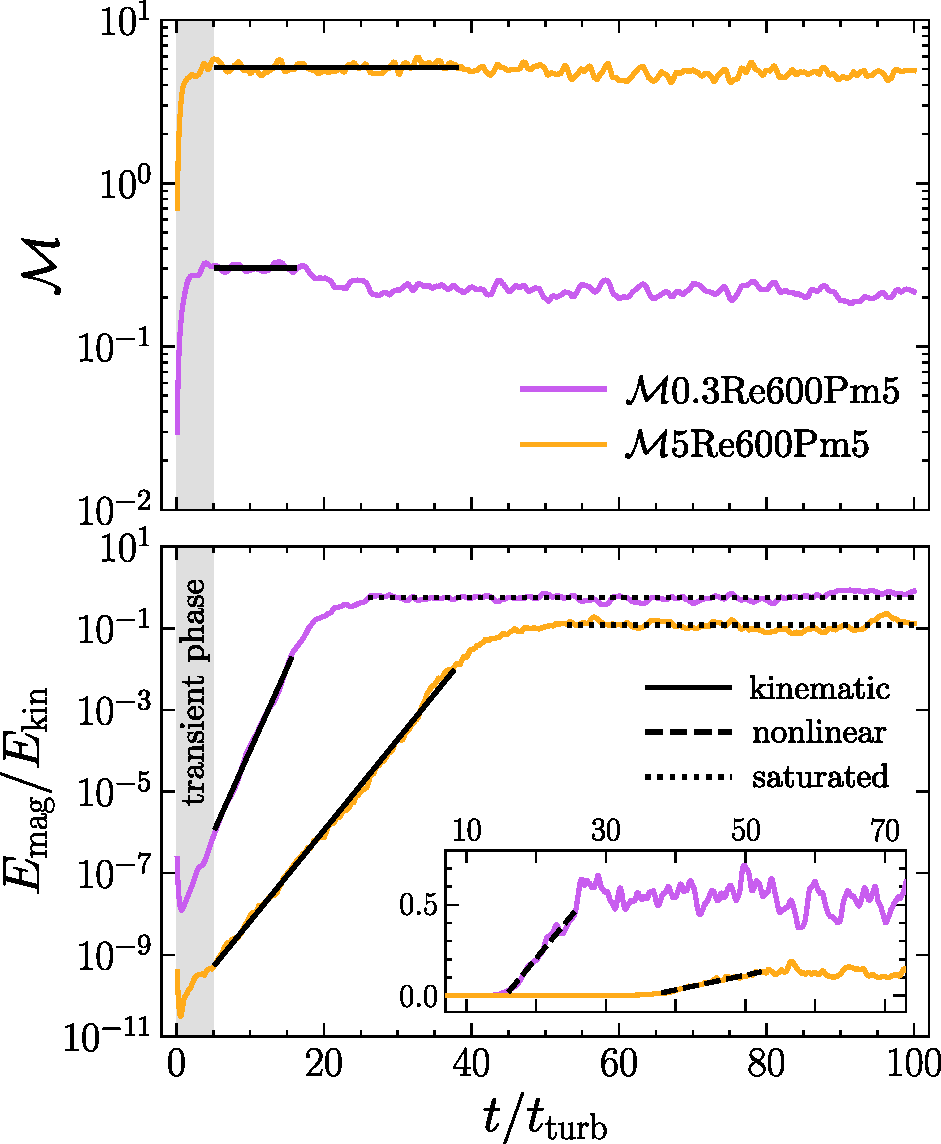
\includegraphics[width=0.65\linewidth]{figures/ssd-exp/time_evolution_updated.pdf}
    \caption{
    Time evolution of the root-mean-squared sonic Mach number ($\mSonicMach$; top panel) and the ratio of the volume-integrated magnetic to kinetic energy ($E_\mathrm{mag}/E_\mathrm{kin}$; bottom panel) for \SimName{0.3}{600}{5} (purple) and \SimName{5}{600}{5} (yellow). Both plasmas have $\mReh = 600 > \mReh_\mathrm{crit} \approx 100$ and $\mPrm = 5$, but $\mSonicMach = 0.3$ and $5$, respectively. We indicate four distinct phases in the simulations: (1) a transient phase where the turbulent velocity field becomes fully established (grey shaded region); (2) a kinematic phase when the magnetic field grows exponentially in time (black solid lines show fits of an exponential model); (3) a polynomial-growth phase that begins once magnetic fields are strong enough to suppress some of the kinetic motions (dashed black lines in the inset panel show linear fits); (4) a saturated phase that begins once the magnetic energy is close to equipartition with the kinetic energy (dotted horizontal lines). We report the measured exponential growth rate, and saturated energy ratio for each of our simulation setups in columns (8) and (9) of \autoref{table:ssd-exp:summary}, respectively.
    }
    \label{fig:time_evolution}
\end{figure}

In \autoref{fig:time_evolution} we plot the time evolution of the rms $\mSonicMach$ and volume-integrated ratio of magnetic to kinetic energy,
\begin{align}
    E_\mathrm{ratio}
        \equiv \frac{
                E_\mathrm{mag}
            }{
                E_\mathrm{kin}
            }
        = \frac{
                \int_{\mVolume} b^2 / (8\pi) \,\mdd\mVolume
            }{
                \int_{\mVolume} \rho u^2 / 2 \,\mdd\mVolume
            }
\end{align}
for two representative simulations, \SimName{0.3}{600}{5} in purple and \SimName{5}{600}{5} in yellow. These runs have identical plasma numbers, $\mReh = 600$ with $\mPrm = 5$, but differ in $\mSonicMach$. In both simulations shown, and in fact for all our simulations (see \autoref{table:ssd-exp:summary}), we identify four distinct phases: a transient phase at the start of the simulation, immediately followed by the kinematic, nonlinear, and finally, maintained phase.

The transient phase roughly spans \DIFdelbegin \DIFdel{$0 \leq t/t_0 \leq 5$}\DIFdelend \DIFaddbegin \DIFadd{$0 \leq t/t_\mathrm{turb} \leq 5$}\DIFaddend , and may be a mixture of the time it takes for our imposed forcing field to accelerate the plasma into a fully developed (statistically stationary) turbulent state, or the so-called diffusion-free regime, where the magnetic field itself moves down to the resistive scale \citep{schekochihin2002spectra}. During this initial phase, the magnetic field reorganises itself out of its initial configuration, and in the case of subsonic turbulence, into a self-similar configuration that has most of its energy concentrated on the smallest scales (\eg \citetalias{kriel2022fundamental} and \citealt{beattie2022growth}). However, we do not focus on this initial, potentially diffusion-free phase, and instead move directly to the classical kinematic stage, which is the focus of this \DIFdelbegin \DIFdel{study}\DIFdelend \DIFaddbegin \DIFadd{chapter}\DIFaddend .

Once the magnetic field progresses past the initial transient state, we see the onset of the kinematic phase. Here, $E_\mathrm{mag}$ grows exponentially fast, amplifying the magnetic energy by more than 7~orders of magnitude, until it reaches $\sim 10\%$ of the kinetic energy. We measure the growth rate, $\gamma$, of magnetic energy during this phase by fitting each simulation with an exponential model, $E_\mathrm{mag}(t) \sim \exp(\gamma t)$, over the time range \DIFdelbegin \DIFdel{$5t_0 \leq t \leq t_\mathrm{end}$}\DIFdelend \DIFaddbegin \DIFadd{$5t_\mathrm{turb} \leq t \leq t_\mathrm{end}$}\DIFaddend , where $t_\mathrm{end}$ is implicitly defined as the time when $E_\mathrm{ratio}(t_\mathrm{end}) = 10^{-2}$. For the two simulations shown, namely \SimName{0.3}{600}{5} and \SimName{5}{600}{5}, we measure growth rates \DIFdelbegin \DIFdel{$\gamma = (1.00 \pm 0.01)t_{0}^{-1}$ and $\gamma = (0.44 \pm 0.01)t_{0}^{-1}$}\DIFdelend \DIFaddbegin \DIFadd{$\gamma = (1.00 \pm 0.01)t_\mathrm{turb}^{-1}$ and $\gamma = (0.44 \pm 0.01)t_\mathrm{turb}^{-1}$}\DIFaddend , and report the measured $\gamma$ for all of our simulations in column 8 of \autoref{table:ssd-exp:summary}. Inspection of these values support the idea that at fixed $\mReh$ and $\mPrm$, $\gamma$ is generally lower in supersonic compared with subsonic SSDs \citep[see, \eg][for more detailed analysis on this effect]{federrath2011mach, schober2012magnetic, federrath2014turbulent, chirakkara2021efficient}. During this (kinematic) phase we also confirm that $\mSonicMach$ remains statistically stationary, and within $5\%$ of our desired value for all our simulations; $\mSonicMach = 0.31 \pm 0.01$ for \SimName{0.3}{600}{5}, and $\mSonicMach = 5.0 \pm 0.2$ for \SimName{5}{600}{5} (see column 7 of \autoref{table:ssd-exp:summary} for all other simulations).

Following the kinematic phase, the magnetic energy growth transitions from an exponential to secular (formally polynomial-in-time \DIFaddbegin \DIFadd{\mbox{%DIFAUXCMD
\citep{beresnyak2012universal, cho2009growth}}\hskip0pt%DIFAUXCMD
}\DIFaddend , but we find it is approximately linear) for both $\mSonicMach <1$ and $\mSonicMach \geq 1$ SSDs. To illustrate this, we plot $E_\mathrm{ratio}$ for our two representative simulations on a linear-linear scale in the inset axis of the bottom panel in \autoref{fig:time_evolution}. Here, for our $\mSonicMach \geq 1$ SSDs, we do not find evidence for a transition into quadratic growth, as has been suggested should be the case by \citet{Schleicher2013_quadratic_growth}. Moreover, as was the case in the kinematic phase, we find that the growth rate in the nonlinear phase is lower for the supersonic, \ie \SimName{5}{600}{5}, compared with the subsonic, \ie \SimName{0.3}{600}{5}, SSDs, which is not directly predicted by any linear growth model based on the energy flux of the hydrodynamical cascade \DIFdelbegin \DIFdel{\mbox{%DIFAUXCMD
\citep[e.g.,]{Xu2016_dynamo,StOnge2020_weakly_collisional_dynamo,beattie2023bulk}}\hskip0pt%DIFAUXCMD
}\DIFdelend \DIFaddbegin \DIFadd{\mbox{%DIFAUXCMD
\citep[e.g.,][]{Xu2016_dynamo,StOnge2020_weakly_collisional_dynamo,beattie2023bulk}}\hskip0pt%DIFAUXCMD
}\DIFaddend . Interestingly, for all of our simulations we find that the duration of the kinematic and nonlinear growth phases are roughly equal. While the duration of the kinematic phase decreases (as the exponential growth rate increases) with plasma numbers (\ie $\mReh$ and $\mPrm$), the duration of the nonlinear phase also decreases by a proportional amount.

Finally, once the magnetic energy approaches equipartition with the kinetic energy, the energy ratio saturates, and is maintained thereafter at a nearly constant value by the forcing field; this defines the saturated phase. We measure \DIFdelbegin \DIFdel{$(E_\mathrm{ratio})_\mathrm{s}at = 0.43 \pm 0.05$ }\DIFdelend \DIFaddbegin \DIFadd{$(E_\mathrm{ratio})_\mathrm{s} = 0.43 \pm 0.05$ }\DIFaddend and $0.07 \pm 0.01$ for \SimName{0.3}{600}{5} and \SimName{5}{600}{5}, respectively, and report this ratio for all simulations in column~9 of \autoref{table:ssd-exp:summary}. Again, these values are generally smaller in the supersonic compared with subsonic regimes.

\subsection{Magnetic Structures}
\label{sec:results:field_slices}

\begin{figure}
    \centering
    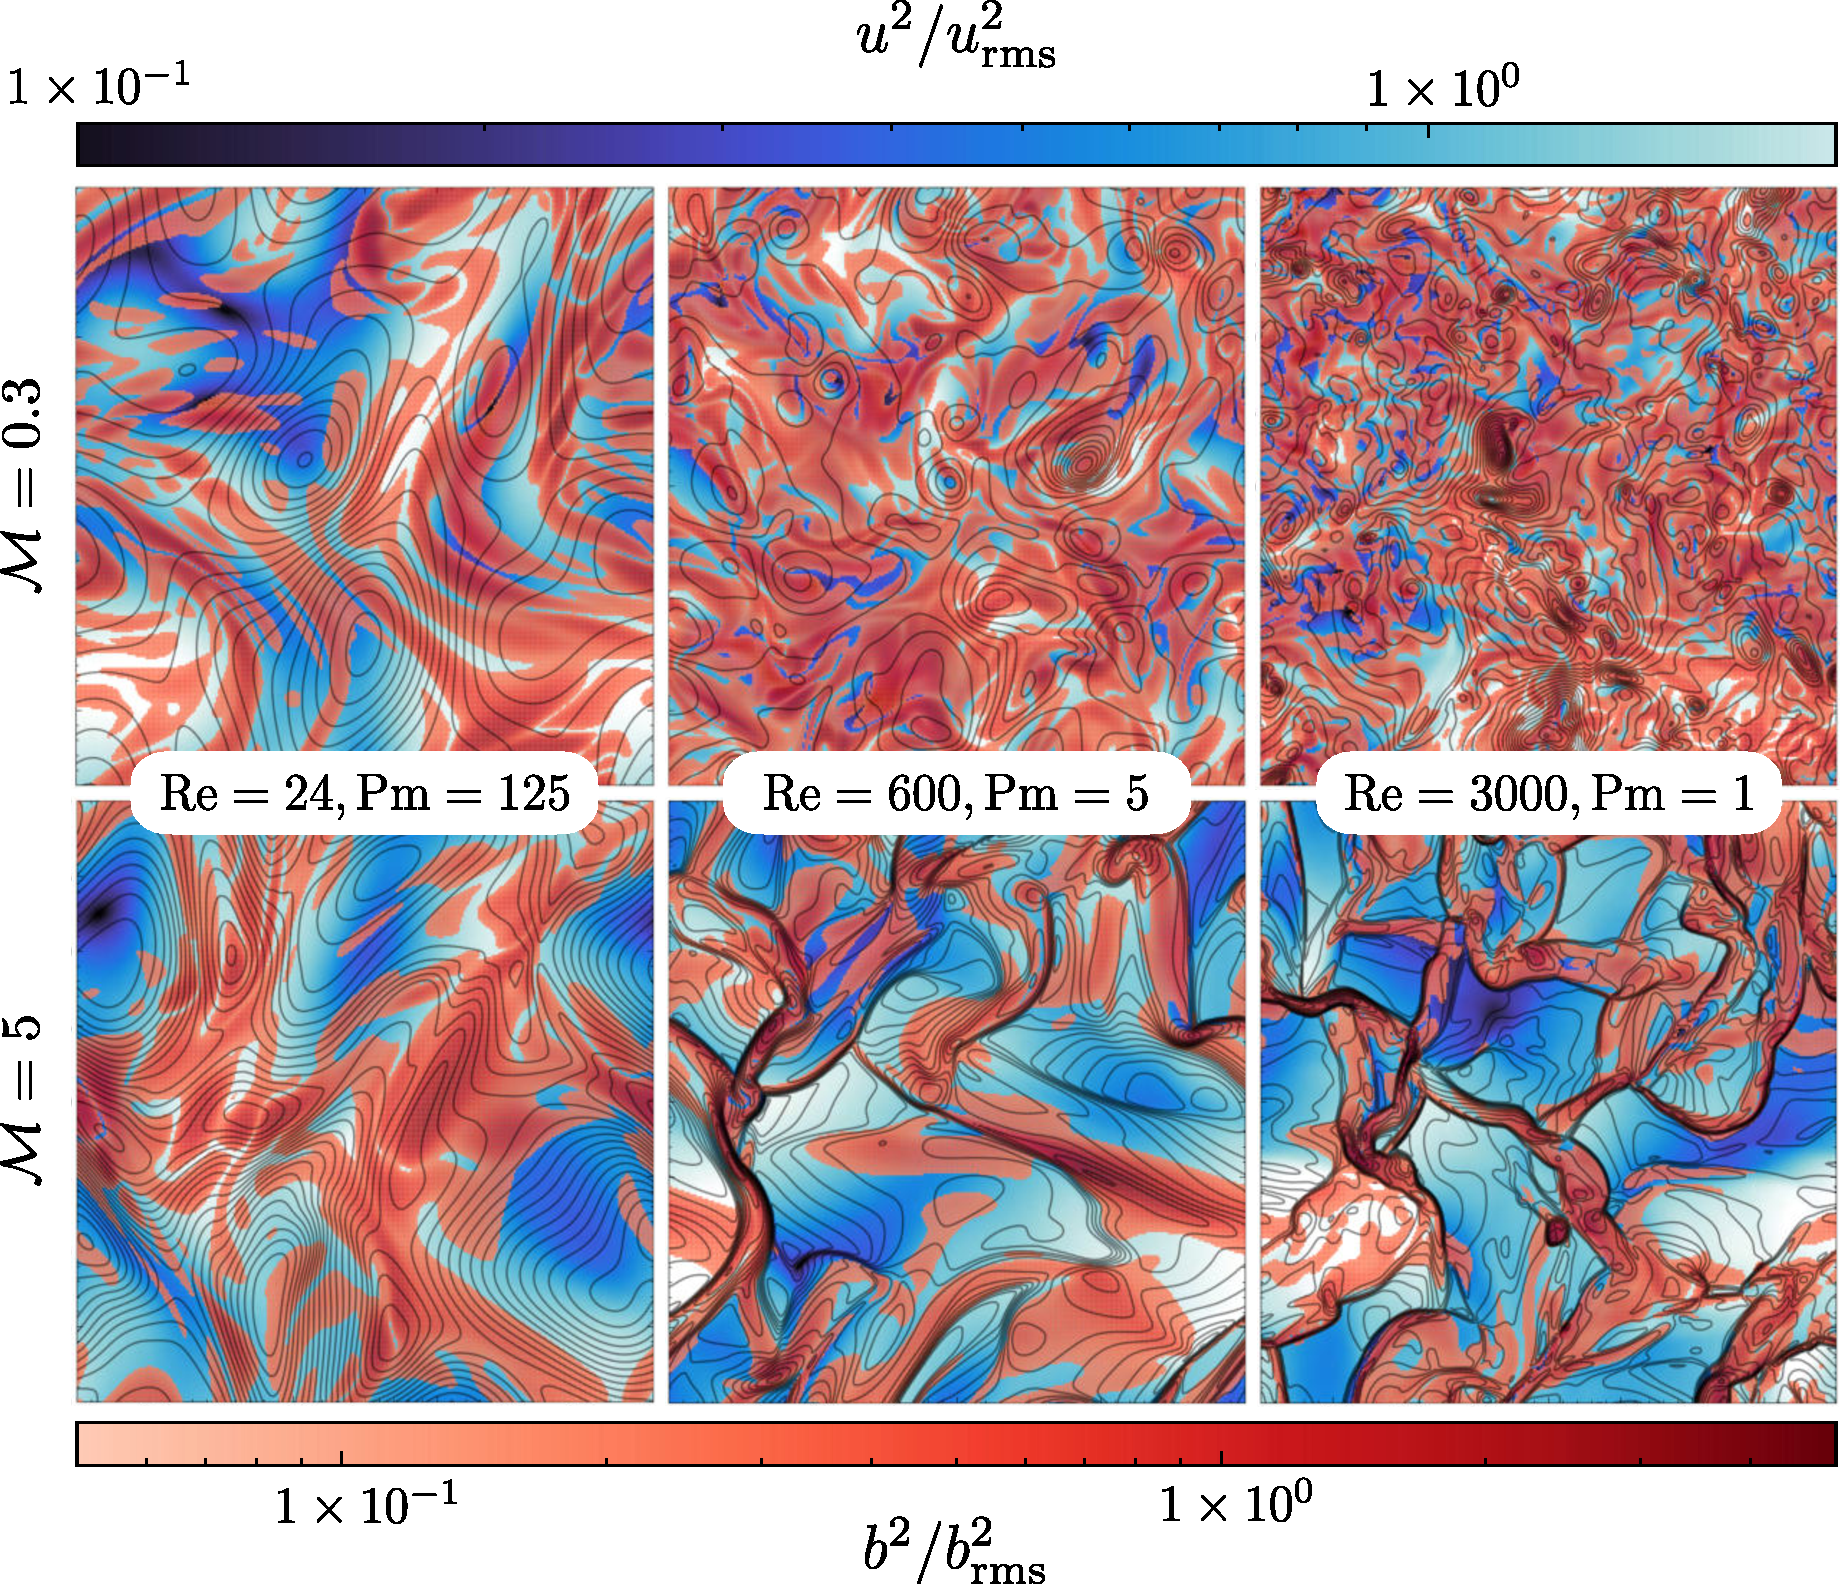
\includegraphics[width=\linewidth]{figures/ssd-exp/field_slices.pdf}
    \caption{Two-dimensional slices of $u^2/u_\mathrm{rms}^2$ (blue), $b^2/b_\mathrm{rms}^2$ (red), and $\rho/\rho_\mathrm{rms}$ (black contours) fields for six different simulations at $N_\mathrm{res} = 576$, spanning a range of plasma regimes. Note that the colourbar for $b^2/b_\mathrm{rms}^2$ is transparent for values $b^2/b_\mathrm{rms}^2 < 0.5$, so regions of low magnetic energy density are not visible. The six simulations shown are \SimName{0.3}{24}{125}, \SimName{0.3}{600}{5}, and \SimName{0.3}{3000}{1} in the top row, and \SimName{5}{24}{125}, \SimName{5}{600}{5}, and \SimName{5}{3000}{1} in the bottom row, respectively, where all simulations have $\mRem = 3000$, with $\mPrm$ (and therefore also $\mReh$) changing, and velocity flows are subsonic ($\mSonicMach = 0.3$) in the top row, and supersonic ($\mSonicMach = 5$) in the bottom row. We see that in the viscous flow regime ($\mReh < \mReh_\mathrm{crit} \approx 100$; left column), both the subsonic and supersonic simulations produce similar, large-scale magnetic structures. Moving towards the turbulent regime ($\mReh \gg \mReh_\mathrm{crit}$; middle and right columns), structures that carry most of the magnetic field energy live on significantly smaller scales compared with the viscous regime. In the subsonic regime (top row), magnetic fields are more uniformly distributed and space-filling, occupying even smaller scales than in the corresponding supersonic simulations (bottom row). In the supersonic simulations, magnetic fields are concentrated in high-density shocked regions bounded by sharp jumps in the velocity magnitude, with an almost constant characteristic length of approximately \DIFdelbeginFL \DIFdelFL{$\ell_0$}\DIFdelendFL \DIFaddbeginFL \DIFaddFL{$\ell_\mathrm{turb}$}\DIFaddendFL , and shock width $\ell_\mathrm{shock}$ decreasing with increasing $\mReh$.}
    \label{fig:field_slices}
\end{figure}

Now that we have confirmed we observe SSD growth in all of our simulations, we turn our attention to field morphologies that are produced during the kinematic phase. In \autoref{fig:field_slices} we plot 2D field slices for six simulations from \autoref{table:ssd-exp:summary} (with the two simulations in \autoref{fig:time_evolution} plotted in the two middle column-panels). All slices are taken from the middle of the simulation domain, $(x, y, z=\ell_\mathrm{box}/2)$, at a time realisation midway through the kinematic phase, \viz $(5 + t_\mathrm{end})/2$, where $t_\mathrm{end}$ is defined as in the previous section. The top and bottom row panels show slices for simulations in two different $\mSonicMach$ regimes, where the top row shows subsonic simulations with $\mSonicMach = 0.3$, and the bottom row shows supersonic simulations with $\mSonicMach = 5$. For all simulations in this figure, we keep \mbox{$\mRem = 3000$} fixed, and vary $\mPrm$ (and thereby $\mReh$, or more explicitly\footnote{
    Because \DIFdelbegin \DIFdel{$\ell_0$ }\DIFdelend \DIFaddbegin \DIFadd{$\ell_\mathrm{turb}$ }\DIFaddend and \DIFdelbegin \DIFdel{$u_0$ }\DIFdelend \DIFaddbegin \DIFadd{$u_\mathrm{turb}$ }\DIFaddend is fixed in each row.
} $\nu$) between the columns.

In the left column we show two simulations in the viscous-flow regime, where $\mReh = 24 < \mReh_\mathrm{crit}$, in the middle column we show mildly turbulent flows, $\mReh = 600 \gtrsim \mReh_\mathrm{crit}$, and the right column we show highly turbulent flows, $\mReh = 3000 \gg \mReh_\mathrm{crit}$. In each panel we plot $u^2 / u_\mathrm{rms}^2$ in blue, $b^2/b_\mathrm{rms}^2$ in red, and $\rho/\rho_\mathrm{rms}$ contours in black, where we have normalised both the velocity and magnetic fields by their rms values to reveal the underlying structure. Note that we truncate the magnetic energy colourbar to only show regions where $b^2/b_\mathrm{rms}^2 > 0.5$, so that the weak-field regions are not shown (\ie transparent).

Qualitatively, the top row of \autoref{fig:field_slices} showcases how the distribution of magnetic energy in subsonic plasmas shifts from being primarily present in large-scale structures in viscous flows (top-left panel), to smaller scale structures in turbulent flows (top-right panel). This systematic transition is characteristic of subsonic SSDs during the kinematic phase, where magnetic fields become stretched, folded, and ultimately organised with most of their energy concentrated at the smallest available scales allowed by Ohmic dissipation.

This is understood to be the result of viscous-scale kinetic fluctuations that most rapidly stretch the magnetic field, giving rise to subviscous magnetic structures that are relatively straight, and become increasingly interspersed with regions of field reversals on smaller scales. \citet{kazantsev1968} showed that the eigenfunction of the induction equation during the kinematic phase of a subsonic SSD, assuming a balance between field stretching and diffusion, leads to a $\ell^{-3/2}$ self-similar scaling of magnetic energy that concentrates energy at the resistive scale. \citet{schekochihin2004simulations} further predicted that the scale on which the magnetic field becomes dominated by dissipation is determined by the balance of the viscous-scale stretching rate and magnetic dissipation rate (more on this in \S\ref{sec:results:dissipation:keta}), which yields $\ell_\mathrm{p} \sim \ell_\eta \sim \ell_\nu \,\mPrm^{-1/2}$. In \citetalias{kriel2022fundamental} we confirmed this predicted scaling using DNSs of subsonic SSDs with resolved physical dissipation, and also measured power-law exponents of the magnetic energy that was consistent with $\ell^{-3/2}$.

Our subsonic simulations (\eg top row of \autoref{fig:field_slices}) once again align with this picture. Here we see that as $\mReh$ increases and $\ell_\nu \sim \mReh^{-3/4}$ shifts to smaller scales, the flow becomes increasingly more turbulent, supporting smaller scale kinetic fluctuations. These turbulent motions give rise to magnetic structures that are significantly smaller scale than the kinetic motions, via the process we described above. For constant $\mReh$ subsonic plasmas, one also expects to see smaller scale magnetic structures emerge, since $\ell_\mathrm{p} \sim \mRem^{1/2}$, however, here our choice to highlight simulations where $\mRem = 3000$ is fixed, is to demonstrate the effect of viscosity, which will become important in \S\ref{sec:results:peak}.

Now, in the supersonic regime (bottom row of \autoref{fig:field_slices}), we observe the magnetic morphology converge on a completely different configuration in the transition from viscous to turbulent plasmas. While both the subsonic and supersonic plasmas shown in the viscous regime (left column) have similar large-scale magnetic structures, the highly turbulent plasmas (right column) produce distinctively different energy distribution patterns. The turbulent, subsonic plasma (top-right panel) produces significantly smaller-scale magnetic energy structures compared with the turbulent, supersonic plasma (bottom-right panel), where magnetic energy becomes primarily concentrated in elongated, coherent, shocked regions of gas, as illustrated by the tightly-packed density contours that coincide with the boundaries of plasma regions where the magnetic energy is strongest.

Embedded within these shocked structures, we still observe sub-structures that appear to have field correlations similar to the subsonic plasma. However, in addition to the smallest scale field structures associated with magnetic dissipation, we now see the emergence of another, larger, scale in the magnetic energy distribution, which appears to be associated with shocks. This scale appears to vary across the supersonic simulations, despite all the supersonic runs being forced on the same scale and with the same strength (\DIFdelbegin \DIFdel{$k_0 = 2$ }\DIFdelend \DIFaddbegin \DIFadd{$k_\mathrm{turb} = 2$ }\DIFaddend and $\mSonicMach = 5$). This suggests that the location of the second scale depends not just on turbulent driving, but also on the visco-resistive properties of the plasma.

While there exist a number of systematic studies of the volume-averaged SSD properties (\eg growth rate and saturated energy ratio) across this transition in the supersonic regime \citep[see for example][]{federrath2011mach, chirakkara2021efficient}, a direct, systematic study of the underlying magnetic field properties has yet to be performed, and therefore we focus on this aspect for the remainder of this \DIFdelbegin \DIFdel{study}\DIFdelend \DIFaddbegin \DIFadd{chapter}\DIFaddend .

\subsection{Measuring Characteristic Scales from Energy Spectra}
\label{sec:results:tools}

To understand the differences in magnetic field characteristic scales that we saw visually in the previous section, we now quantify three key characteristic scales: the size of viscous fluctuations ($\ell_\nu$), which most dominantly drive SSD amplification during the kinematic phase of subsonic SSDs; the resistive scale ($\ell_\eta$), where Ohmic dissipation becomes significant; and the scale where magnetic energy is concentrated ($\ell_\mathrm{p}$). By establishing a relationship between these scales and plasma parameters (\eg $\mSonicMach$, $\mReh$, and $\mPrm$), we aim to compare and contrast subsonic and supersonic plasma SSDs, thereby shedding light on how amplification differs in supersonic SSDs compared with their subsonic counterparts.

Since the flows we are studying are homogeneous and isotropic, we study characteristic scales in Fourier space, where length-scales and wavenumbers are directly related ($k \equiv 2\pi / \ell$). In \citetalias{kriel2022fundamental}, we measured characteristic wavenumbers from our simulations by fitting semi-analytical models for the kinetic ($E_\mathrm{kin}(k)$) and magnetic ($E_\mathrm{mag}(k)$) energy spectra. These spectra were derived from 1D shell-integrated power spectra calculated from our simulations in the usual way of summing the total power in discrete, radial shells in k-space. More explicitly, the energy spectrum of field $\mVector{\psi}$ is computed as
\begin{align}
    E_\psi(k, t)
        = \sum_{k^* < \|\mVector{k}\| < k^* + \Delta k^*}
            4\pi k^2 \widetilde{\psi}(\mVector{k}, t) \, \widetilde{\psi}^*(\mVector{k}, t)
\end{align}
where we choose to bin in integer $k$-bins ($k^* \in \mathds{Z}^+ : k^* \ne 0$) separated by $\Delta k^* = 1$, and
\begin{align}
    \widetilde{\psi}(\mVector{k}, t)
        = \frac{1}{(2 \pi \ell_\mathrm{box})^{3/2}} \int_\mVolume \psi(\mVector{\ell}, t) \exp\rbrac{-i \mVector{k}\cdot\mVector{\ell}} \,\mdd{^3 \ell}
        \label{eqn:kin_fourier}
\end{align}
is the Fourier transform of $\psi(\mVector{\ell}, t)$, with $\widetilde{\psi}^*(\mVector{k}, t)$ its complex conjugate.

We also attempted this \DIFaddbegin \DIFadd{same model-fitting }\DIFaddend approach for the present study, but found that the existing functional models for both energy spectra fail to reliably measure characteristic scales in our supersonic simulations, especially in lower-resolution runs, which were necessary to perform our resolution study. Two main issues arose: (1) due to the limited inertial range for our low-$\mReh$ simulations, we could not effectively constrain $k_\nu$; (2) supersonic simulations had a broader energy spectrum than the subsonic simulations, which was not well-fit by the functional form we had used in \citetalias{kriel2022fundamental} (\ie the $E_{\mathrm{mag}}(k)$ model originally derived by \citet{kulsrud1992spectrum} for a magnetic field coupled to a delta-correlated in time velocity field during the kinematic phase of a subsonic, $\mPrm \gg 1$ SSD). Furthermore, at very high-$\mReh$, as shown in \citet{Beattie2024_10k_MHD}, if there are break scales in the spectrum it is not obvious what the dissipation scales should be if derived directly from a fit.

Prompted by these challenges, we develop new and simpler, spectral model-free methods for measuring $k_\nu$, $k_\eta$, and $k_\mathrm{p}$, based on the underlying turbulence and fluid physics theory, which we apply to all our simulations, and demonstrate yields robust results for all plasma and flow regimes.

\subsubsection{Characteristic Viscous Wavenumber}
\label{sec:tools:k_nu}

\begin{figure}
    \centering
    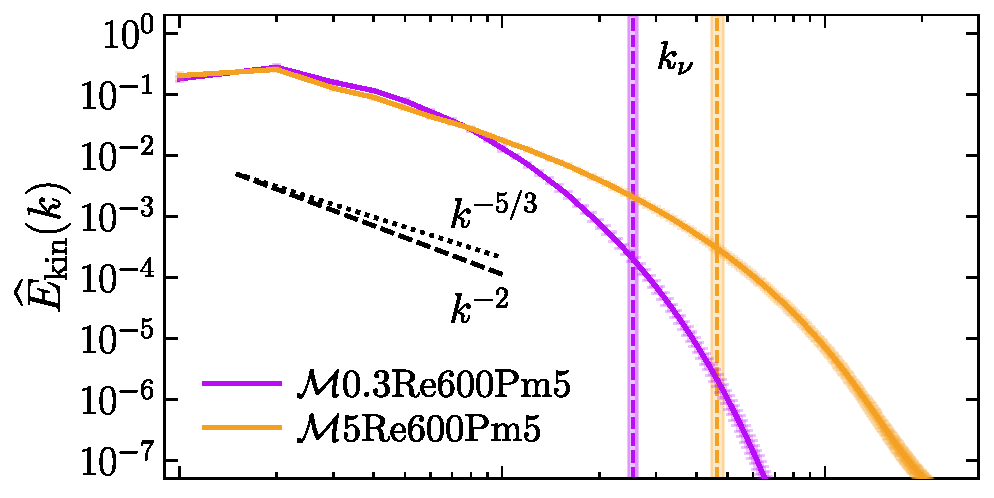
\includegraphics[width=0.65\linewidth]{figures/ssd-exp/spectra_kin.pdf}
    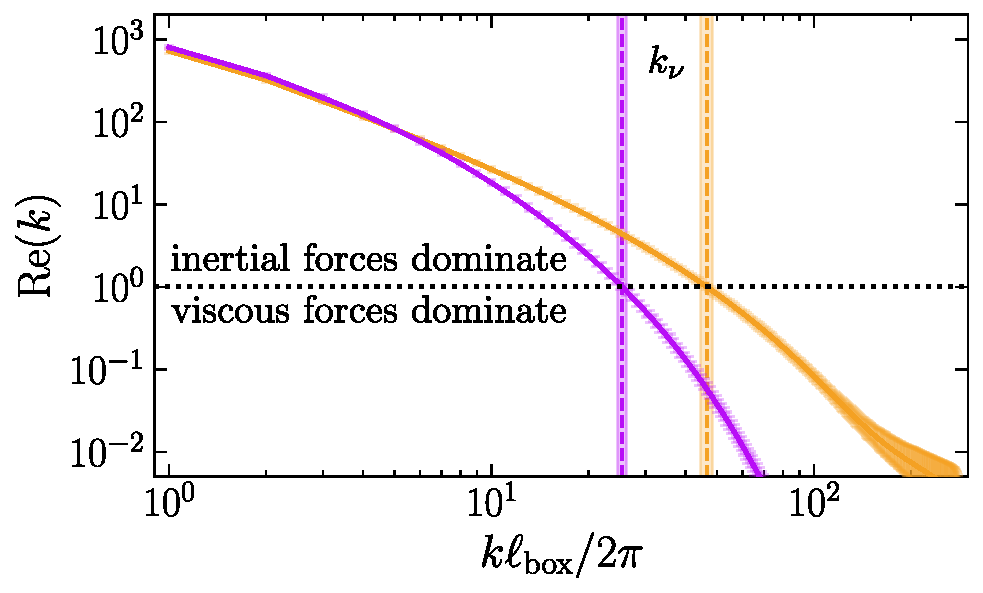
\includegraphics[width=0.65\linewidth]{figures/ssd-exp/spectra_reynolds.pdf}
    \caption{Normalised and time-averaged (over the kinematic phase) kinetic energy spectrum ($\widehat{E}_\mathrm{kin}(k)$; top panel) constructed with $\mVector{\psi} = \mVector{u} / \sqrt{2}$ in \autoref{eqn:kin_fourier}, for the \SimName{0.3}{600}{5} (purple) and \SimName{0.3}{600}{5} (yellow) simulations run at $N_\mathrm{res} = 576$. The solid lines shows the $50^\mathrm{th}$ percentile of the $\widehat{E}_\mathrm{kin}(k)$ spectrum over all snapshots during this phase, and the bands show the $16^\mathrm{th}$ to $84^\mathrm{th}$ percentile variance of $\widehat{E}_\mathrm{kin}(k)$. We also plot the wavenumber-dependent hydrodynamic Reynolds number ($\mReh(k)$ computed via \autoref{eqn:reynolds_spectrum}; bottom panel). From $\mReh(k)$ we measure a characteristic kinetic energy dissipation (viscous) wavenumber ($k_\nu: \mReh(k_\nu) = 1$ via \autoref{eqn:knu_measure}), which we annotate with vertical lines for both simulations in the top and bottom panels. For reference, we also plot $\widehat{E}_\mathrm{kin}(k) \sim k^{-5/3}$ and $\widehat{E}_\mathrm{kin}(k) \sim k^{-2}$ in the top panel, which corresponds with the expected inertial range scaling of \citet{kolmogorov1941dissipation} and \citet{burgers1948_turbulence_model} kinetic energy spectra, respectively.}
    \label{fig:kin_spectra}
\end{figure}

\begin{figure}
    \centering
    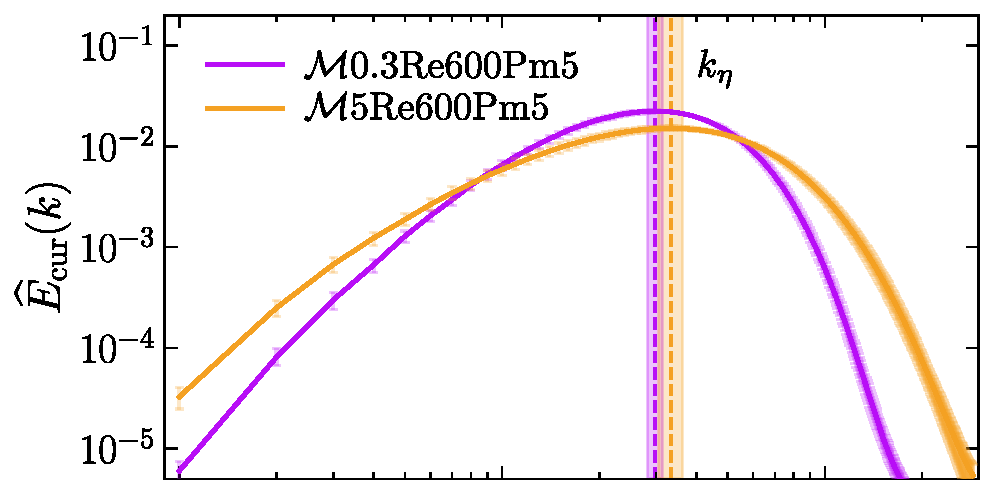
\includegraphics[width=0.65\linewidth]{figures/ssd-exp/spectra_cur.pdf}
    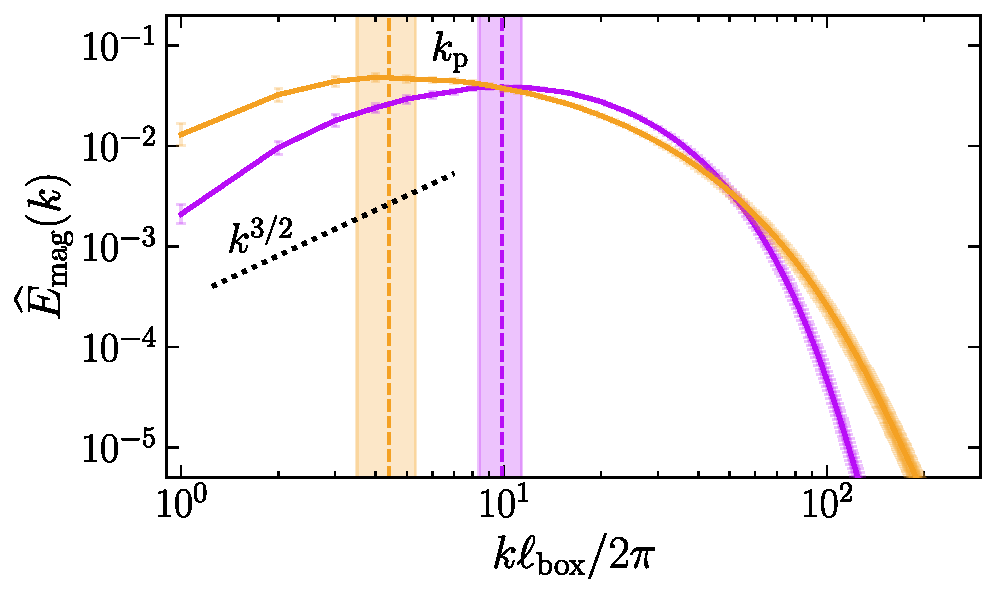
\includegraphics[width=0.65\linewidth]{figures/ssd-exp/spectra_mag.pdf}
    \caption{As in \autoref{fig:kin_spectra}, but for the current density power spectra ($\widehat{E}_\mathrm{cur}(k)$; top panel) and magnetic energy spectrum ($\widehat{E}_\mathrm{mag}(k)$; bottom panel) for \SimName{0.3}{600}{5} and \SimName{5}{600}{5}. We annotate the measured characteristic magnetic dissipation (resistive) wavenumber in the top panel, ($k_\eta$; \autoref{eqn:keta_measure}), and the magnetic peak wavenumber ($k_\mathrm{p}$; \autoref{eqn:kp_measure}), in the bottom panel. We also annotate $\widehat{E}_\mathrm{mag}(k) \sim k^{3/2}$ for reference, which is the expected scaling of $E_\mathrm{mag}(k)$ in the subviscous range during the kinematic phase of a subsonic SSD \citep{kazantsev1968, schekochihin2002model}.}
    \label{fig:cur_mag_spectra}
\end{figure}

We define the viscous wavenumber, $k_\nu$, directly from the definition in Kolmogorov turbulence, \ie the wavenumber where the scale-dependent hydrodynamic Reynolds number equals one, $\mReh(k_\nu) = 1$. This scale marks the transition from inertial forces dominating in the turbulent cascade, \DIFdelbegin \DIFdel{$k_0 < k < k_\nu$}\DIFdelend \DIFaddbegin \DIFadd{$k_\mathrm{turb} < k < k_\nu$}\DIFaddend , to dissipation dominating at \mbox{$k_\nu < k$}. Hence, to measure $k_\nu$, we construct the wavenumber-dependent hydrodynamic Reynolds number,
\DIFdelbegin %DIFDELCMD < \begin{align}
%DIFDELCMD <     \mReh(k, t)
%DIFDELCMD <         = \frac{u_0(k,t)}{\nu k}
%DIFDELCMD <         , \label{eqn:reynolds_spectrum}
%DIFDELCMD < \end{align}%%%
\DIFdelend \DIFaddbegin \begin{align}
    \mReh(k, t)
        = \frac{u_\mathrm{turb}(k,t)}{\nu k}
        , \label{eqn:reynolds_spectrum}
\end{align}\DIFaddend
which follows from the turbulent velocity as a function of $k$,
\DIFdelbegin %DIFDELCMD < \begin{align}
%DIFDELCMD <     u_0 (k, t)
%DIFDELCMD <         = \rbrac{
%DIFDELCMD <             \frac{2}{\rho_0} \int_{k}^{\infty} E_\mathrm{kin}(k^\prime, t) \,\mdd{k^\prime}
%DIFDELCMD <         }^{1/2}
%DIFDELCMD <         . \label{eqn:velocity_k}
%DIFDELCMD < \end{align}%%%
\DIFdelend \DIFaddbegin \begin{align}
    u_\mathrm{turb} (k, t)
        = \rbrac{
            \frac{2}{\rho_0} \int_{k}^{\infty} E_\mathrm{kin}(k^\prime, t) \,\mdd{k^\prime}
        }^{1/2}
        . \label{eqn:velocity_k}
\end{align}\DIFaddend
In practice we solve for $k_\nu$ from our simulations using a root finding method,
\begin{align}
    k_\nu(t)
        = \texttt{argmin}_k\Big[
            \mathcal{I}\Big\{ \Big| \mReh(k, t) - 1 \Big| \Big\}
        \Big]
        , \label{eqn:knu_measure}
\end{align}
where $|\dots|$ is the absolute operator, $\mathcal{I}[\dots]$ is a piecewise cubic polynomial (spline) interpolation operator, as performed in \citet{beattie2022growth}, and $\texttt{argmin}_k[h(k)]$ returns the argument $k$ which minimises the function $h(k)$. For each of our simulations, we evaluate \autoref{eqn:knu_measure} at each time-snapshot during the kinematic phase.

While \autoref{eqn:knu_measure} provides a simple way of extracting the viscous wavenumber from $E_\mathrm{kin}(k)$, there remains the question of which field, $\mVector{\psi}$, to Fourier transform in the supersonic regime. When $\mVector{\psi} = \mVector{u}/\sqrt{2}$ in \autoref{eqn:kin_fourier}, then $E_\mathrm{kin}(k)$ is the velocity power spectrum, which leads \autoref{eqn:reynolds_spectrum} to carry the same units as the usual definition of the hydrodynamic Reynolds number. For incompressible flows, this approach is directly proportional to the kinetic energy spectrum, because the density field is constant. However, this velocity power spectrum definition for $E_\mathrm{kin}(k)$ ignores the covariance between the density field and the square velocity field, \ie $\mAve{\rho u^2}_\mVolume / 2$ (see \autoref{note:naming_convesions}), as well as fluctuations in the density field, which for compressible, isothermal plasmas are a factor of $\mSonicMach$ larger than velocity fluctuations (this factor follows from a unit analysis of the ideal-hydrodynamic momentum equation in steady state). \citet{beattie2020filaments} showed that the density spectrum becomes dominated by high-$k$ modes that can lead to large pressure gradients, which mediate the exchange of kinetic and internal energy \citep[see for example][]{federrath2010comparing, federrath2013universality, schmidt2019kinetic, grete2021matter, grete2023matter}. Therefore, we also check whether density fluctuations affect our measurements of $k_\nu$, by also considering the definition for $E_\mathrm{kin}$ which carries the units of kinetic energy, namely with $\mVector{\psi} = \mVector{u} \sqrt{\rho/2}$ \citep[see, e.g., ][]{federrath2010comparing, grete2021matter, grete2023matter}.

Here, in the main text, we focus on $k_\nu$ derived from \autoref{eqn:reynolds_spectrum} constructed with $\mVector{\psi} = \mVector{u}/\sqrt{2}$, which we demonstrate in \autoref{fig:kin_spectra} for the same two representative simulations shown in \autoref{fig:time_evolution}, namely \SimName{0.3}{600}{5} and \SimName{5}{600}{5}. Then, in \DIFdelbegin \DIFdel{\S\ref{app:knu:density_weighted}}\DIFdelend \DIFaddbegin \DIFadd{End Matter (\S\ref{app:knu:density_weighted})}\DIFaddend , we demonstrate that regardless of the choice of definition for $E_\mathrm{kin}(k)$, whether based on $\mReh(k)$ having dimensionless units (\ie constructed with $\mVector{\psi} = \mVector{u} / \sqrt{2}$), or choosing $\mVector{\psi} = \mVector{u} \sqrt{\rho/2}$ such that $E_\mathrm{kin}(k)$ carries units of kinetic energy, we recover the same scaling behaviour for $k_\nu$, and thus the choice of definition for $E_\mathrm{kin}$ does not affect any of the conclusions presented in our study.

\subsubsection{Characteristic Resistive Wavenumber}
\label{sec:tools:k_eta}

While our approach of defining $k_\nu$ in terms of the wavenumber-dependent hydrodynamic Reynolds number performs well, we find that an analogous approach to defining the resistive wavenumber in terms of the spectrum of $\mRem$ yields results that are inconsistent with those derived from early methods \citep{kulsrud1992spectrum, kriel2022fundamental, brandenburg2023dissipative}; see \DIFdelbegin \DIFdel{\S\ref{app:krm} }\DIFdelend \DIFaddbegin \DIFadd{End Matter (\S\ref{app:krm}) }\DIFaddend for details. For this reason, we adopt a different approach. Recognising that, since we employ Ohmic dissipation in the induction equation (\autoref{mhd:induction}), the magnetic dissipation rate at any point in space is exactly equal to $\eta j^2$. On this basis we define the resistive wavenumber as the wavenumber of maximum $j^2(k)$, corresponding to the maximum magnetic dissipation (since $\eta$ is a constant). Explicitly, we define $k_\eta$ as the value of $k$ corresponding to the maximum of the 1D shell-integrated current density spectrum (which has units of current density squared), $E_\mathrm{cur}(k)$, which is defined similarly to $E_\mathrm{kin}(k)$ in \S\ref{sec:tools:k_nu}, but for the field $\mVector{\psi} = \nabla\times\mVector{b} / (4\pi)$.

In practice we implement this as
\begin{align}
    k_\eta(t)
        = \texttt{argmax}_k\Big[
            \mathcal{I}\Big\{ E_\mathrm{cur}(k, t) \Big\}
        \Big]
        , \label{eqn:keta_measure}
\end{align}
where $\mathcal{I}\{\dots\}$ is defined as in \autoref{eqn:knu_measure}, and $\texttt{argmax}_k[h(k)]$ returns the argument $k$ which maximises $h(k)$. As with $k_\nu$, we compute this quantity for every snapshot during the kinematic phase. We illustrate this procedure in the top panel of \autoref{fig:cur_mag_spectra}, where in analogy with the top panel of \autoref{fig:kin_spectra}, we plot the normalised and time-averaged (over the kinematic phase) $E_\mathrm{cur}$ for our two representative simulations, with the corresponding measured resistive wavenumbers $k_\eta$ indicated with vertical bands.

\subsubsection{Peak Magnetic Wavenumber}
\label{sec:tools:k_p}

Finally, we define the magnetic peak wavenumber as the maximum of $E_\mathrm{mag}(k)$, defined similarly to the current density power spectra but with $\mVector{\psi} = \mVector{b} / {8\pi}$. Explicitly,
\begin{align}
    k_\mathrm{p}(t)
        = \texttt{argmax}_k\Big[
            \mathcal{I}\Big\{ E_\mathrm{mag}(k, t) \Big\}
        \Big]
        . \label{eqn:kp_measure}
\end{align}
We illustrate $E_\mathrm{mag}(k)$ and $k_\mathrm{p}$ for our two representative simulations in the bottom panel of \autoref{fig:cur_mag_spectra}. In \S\ref{app:kcor} we point out that, while the magnetic correlation wavenumber is directly proportional to peak wavenumber during the kinematic phase of a subsonic (both viscous and turbulent) SSD \citep{schekochihin2004simulations, galishnikova2022tearing, beattie2022growth}, this scaling breaks down for supersonic, turbulent SSDs.

\subsection{Convergence of Measured Wavenumbers}
\label{sec:results:nres}

\begin{figure}
    \centering
    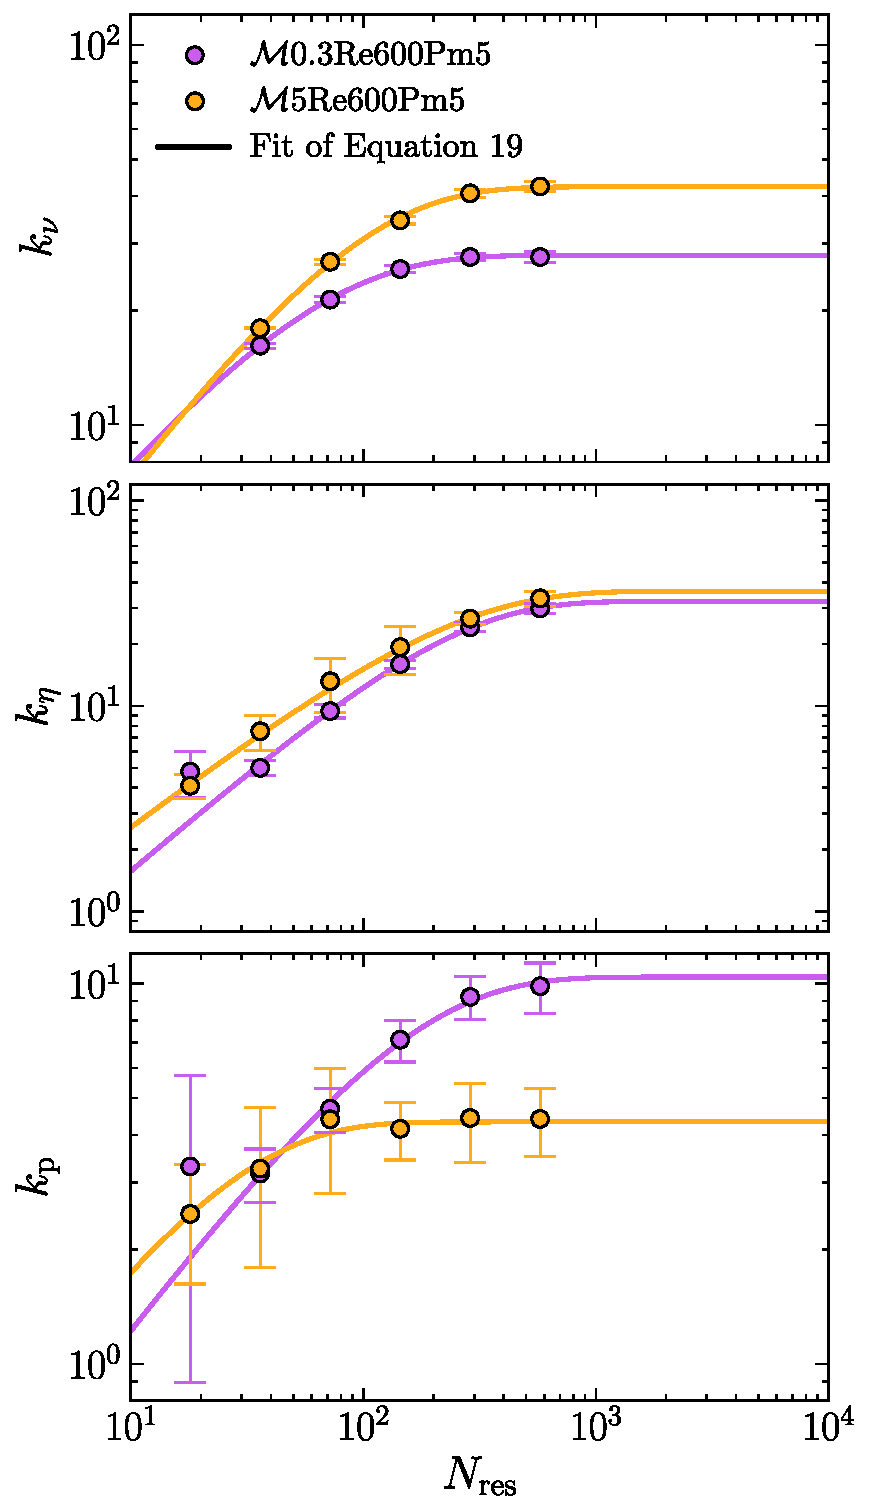
\includegraphics[width=0.65\linewidth]{figures/ssd-exp/nres_scales.pdf}
    \caption{Measured viscous ($k_\nu$; top panel), resistive ($k_\eta$; middle panel), and magnetic peak ($k_\mathrm{p}$; bottom panel) wavenumbers plotted against linear grid resolution for \SimName{0.3}{600}{5} (magenta) and \SimName{5}{600}{5} (yellow) as circles, indicating the 1-sigma standard deviation in the temporal variation of each scale with error-bars. We overlay a best-fit of our convergence model (\autoref{eqn:nres}), to each set of wavenumbers to measure characteristic wavenumbers that have converged with resolution. We report the converged $k_\nu$, $k_\eta$, and $k_\mathrm{p}$ for each of our simulations in columns (10), (11), and (12) of \autoref{table:ssd-exp:summary}, respectively.}
    \label{fig:nres_scales}
\end{figure}

\DIFdelbegin %DIFDELCMD < \begin{figure}
%DIFDELCMD <     \centering
%DIFDELCMD <     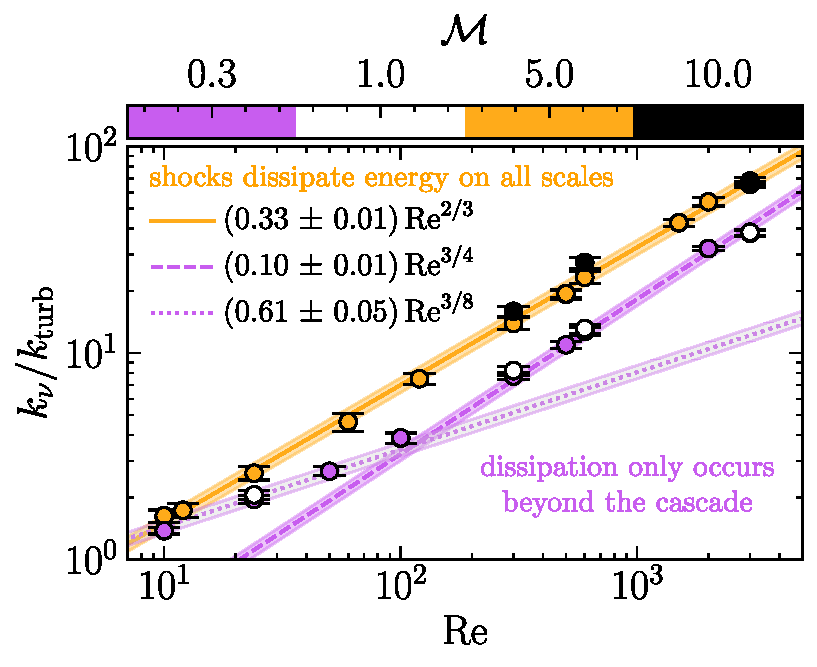
\includegraphics[width=0.49\linewidth]{figures/ssd-exp/scaling_knu_kin_updated.pdf}
%DIFDELCMD <     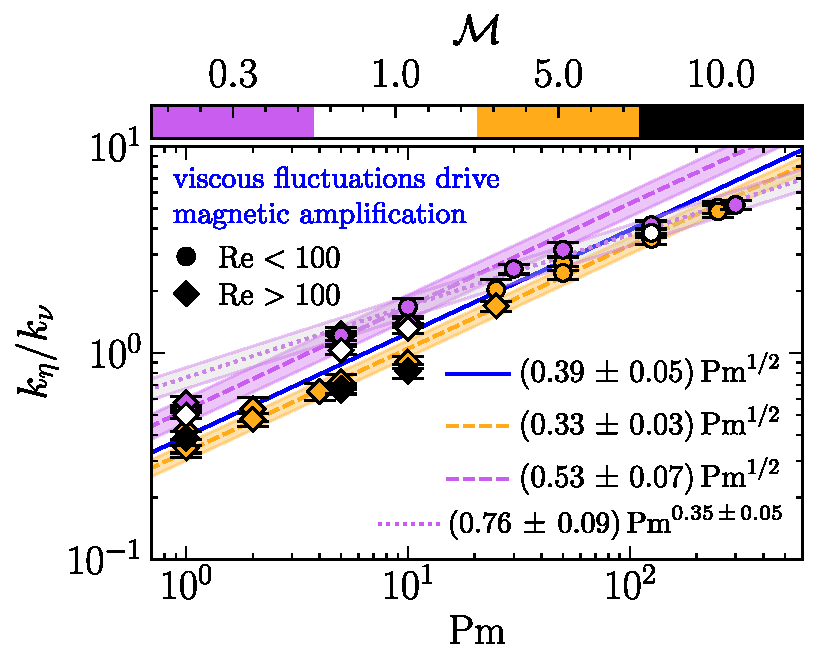
\includegraphics[width=0.49\linewidth]{figures/ssd-exp/scaling_keta_cur_updated.pdf}
%DIFDELCMD <     %%%
%DIFDELCMD < \caption{%
{%DIFAUXCMD
\DIFdelFL{In the left panel we plot the scale separation between the converged kinetic dissipation wavenumber ($k_\nu$) and the external forcing wavenumber ($k_0 = 2$) as a function of the hydrodynamic Reynolds number ($\mReh$) for each simulation setup in }%DIFDELCMD < \autoref{table:ssd-exp:summary}%%%
\DIFdelFL{. In the right panel we also compare the scale separation between the converged magnetic and kinetic dissipation wavenumbers ($k_\eta / k_\nu$) against the magnetic Prandtl number ($\mPrm$). Points are coloured by $\mSonicMach$, where $\mSonicMach = 0.3$ simulations are coloured magenta, $\mSonicMach = 1$ are coloured white, $\mSonicMach = 5$ are coloured yellow, and $\mSonicMach = 10$ are coloured black. To guide the eye in the left panel, we fit theoretical scalings of $k_\nu$ in different flow regimes: $k_\nu \sim \mReh^{2/3}$ to supersonic ($\mSonicMach > 1$) simulations (solid yellow line; expected for \mbox{%DIFAUXCMD
\citealt{burgers1948_turbulence_model} }\hskip0pt%DIFAUXCMD
turbulence), $k_\nu \sim \mReh^{3/4}$ to the turbulent ($\mReh \geq \mReh_\mathrm{crit} \approx 100$) subset of trans- and subsonic ($\mSonicMach \leq 1$) simulations (dashed magenta line; expected for \mbox{%DIFAUXCMD
\citealt{kolmogorov1941dissipation} }\hskip0pt%DIFAUXCMD
turbulence), and $k_\nu \sim \mReh^{3/8}$ to viscous ($\mReh < \mReh_\mathrm{crit}$), trans- and subsonic velocity fields (dotted magenta line; see \mbox{%DIFAUXCMD
\citetalias{kriel2022fundamental}}\hskip0pt%DIFAUXCMD
). In the right panel we plot viscous simulations ($\mReh < \mReh_\mathrm{crit}$) as circles, and turbulent simulations ($\mReh \geq \mReh_\mathrm{crit}$) as diamonds. We also fit a $k_\eta/k_\nu \sim \mPrm^{1/2}$ scaling to the full dataset (solid blue line), the supersonic simulations (dashed yellow line), and the turbulent subset of the trans- and subsonic simulations (dashed magenta line). Finally, we also fit a general power-law model to the viscous subset of trans- and subsonic simulations, and recover a fit (dotted magenta line) that is consistent with our findings in \mbox{%DIFAUXCMD
\citetalias{kriel2022fundamental}}\hskip0pt%DIFAUXCMD
, where the range of subviscous scales has a shallower dependence on $\mPrm$ than in the turbulent regime. We report all fitted parameters and their 1-sigma uncertainties in their respective labels.}}
    %DIFAUXCMD
%DIFDELCMD < \label{fig:dissipation_scaling}
%DIFDELCMD < \end{figure}
%DIFDELCMD <

%DIFDELCMD < %%%
\DIFdelend As previously discussed in \S\ref{sec:ICs:nres}, we ensure that all the characteristic wavenumbers we measure from our different simulation setups are converged with respect to the grid resolution $N_\mathrm{res}$. We do this by running each simulation setup in \autoref{table:ssd-exp:summary} across a wide range of $N_\mathrm{res}$, measuring our three wavenumbers of interest, $k_\mathrm{scale} \in \{k_\nu, k_\eta, k_\mathrm{p}\}$ in the kinematic phase, and then fitting a generalised logistic model of the functional form
\begin{align}
    k_\mathrm{scale}(N_\mathrm{res})
        = k_\mathrm{scale}(\infty) \rbrac{
                1 - \exp\cbrac{ -\rbrac{\frac{N_\mathrm{res}}{N_\mathrm{res, crit}}}^R }
            }
        , \label{eqn:nres}
\end{align}
to the resolution-dependent wavenumbers. The parameters in our fits are $k_\mathrm{scale}(\infty)$, which represents the converged ($N_\mathrm{res} \to \infty$) value of each wavenumber $\{k_\nu, k_\eta, k_\mathrm{p}\}$, the rate of convergence $R$, and the critical resolution $N_\mathrm{res, crit}$ at which characterises the resolution where convergence begins.

As discussed in \S\ref{sec:ICs:nres}, we start by running each simulation configuration across $N_\mathrm{res} = 18 - 288$, separated by factors of 2, and then we fit those data for $N_\mathrm{res,crit}$. If we find that our best-fit value of $N_\mathrm{res,crit}$ is larger than 288, or that our data does not yield a fit for $N_\mathrm{res,crit}$ with reasonable uncertainty, we rerun that setup at the higher resolution $N_\mathrm{res} = 576$. We then repeat the convergence test, doubling the resolution until we obtain a well-constrained value of $N_\mathrm{res,crit}$, such that our highest-resolution run for each setup satisfies $\texttt{max}[\{N_\mathrm{res}\}] > N_\mathrm{res, crit}$.

In \autoref{fig:nres_scales} we plot the resolution ($N_\mathrm{res}$) dependent $k_\nu$, $k_\eta$, and $k_\mathrm{p}$, and our best fits to these wavenumbers, for our two representative simulations. Broadly, for both simulations, we find evidence of convergence at $N_\mathrm{res} \approx 576$, but since $k_\nu$, $k_\eta$, and $k_\mathrm{p}$ may all exist on different scales, one would expect the convergence properties of each wavenumber to be different, since small-scale (high-$k$) structures are expected to require higher resolution to converge than larger-scale (low-$k$) structures. This is what we find. For \SimName{0.3}{600}{5} we find $k_\nu$ begins to converge at $N_\mathrm{res, crit} = 43.0 \pm 2.2$, while $k_\eta$ and $k_\mathrm{p}$ begin converging at $N_\mathrm{res, crit} = 190.4 \pm 20.2$ and $N_\mathrm{res, crit} = 117.2 \pm 40.0$, respectively. This is expected, since we are operating in the $\mPrm \geq 1$ regime where magnetic structures are smaller-scale than velocity structures, \viz \mbox{$k_\nu < k_\eta \sim k_\mathrm{p}$}, and therefore require a higher grid resolution to resolve. By contrast, for \SimName{5}{600}{5}, we find that $k_\nu$ shows convergence at $N_\mathrm{res, crit} = 79.4 \pm 4.6$, whereas $k_\eta$ requires $N_\mathrm{res, crit} = 173.5 \pm 40.7$ and $k_\mathrm{p}$ requires $N_\mathrm{res, crit} = 20.6 \pm 18.3$. Comparing the subsonic and supersonic cases, it is noteworthy that $k_\eta$ shows similar convergence behaviour, but that $k_\mathrm{p}$ converges at significantly lower grid resolution, consistent with the visual differences in size-scale visible in \autoref{fig:field_slices}.

We report the converged values $k_\mathrm{scale}(\infty)$ (extrapolated to infinite resolution) for all our simulations in columns 10--12 of \autoref{table:ssd-exp:summary}, and use this in all of our analysis that follows, but for compactness from this point on (and in the header of \autoref{table:ssd-exp:summary}) we drop the notation $(\infty)$. We also report the measured $N_\mathrm{res, crit}$ and $R$ for all three derived characteristic wavenumbers, from each of our simulations, in \autoref{table:ssd-exp:nres}. These fits are based on using all data up to the highest resolution we have run for each simulation configuration.

\DIFaddbegin \begin{figure}
    \centering
    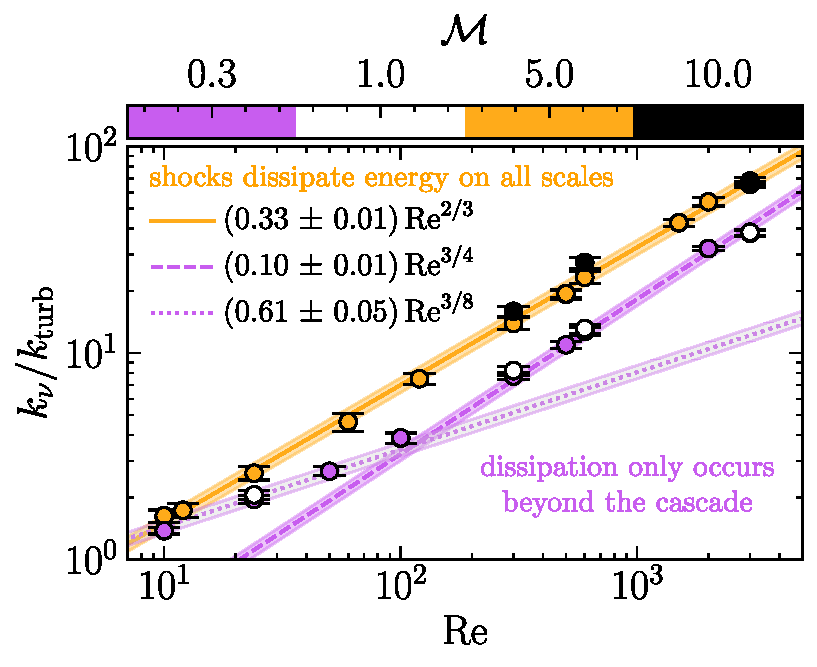
\includegraphics[width=0.49\linewidth]{figures/ssd-exp/scaling_knu_kin_updated.pdf}
    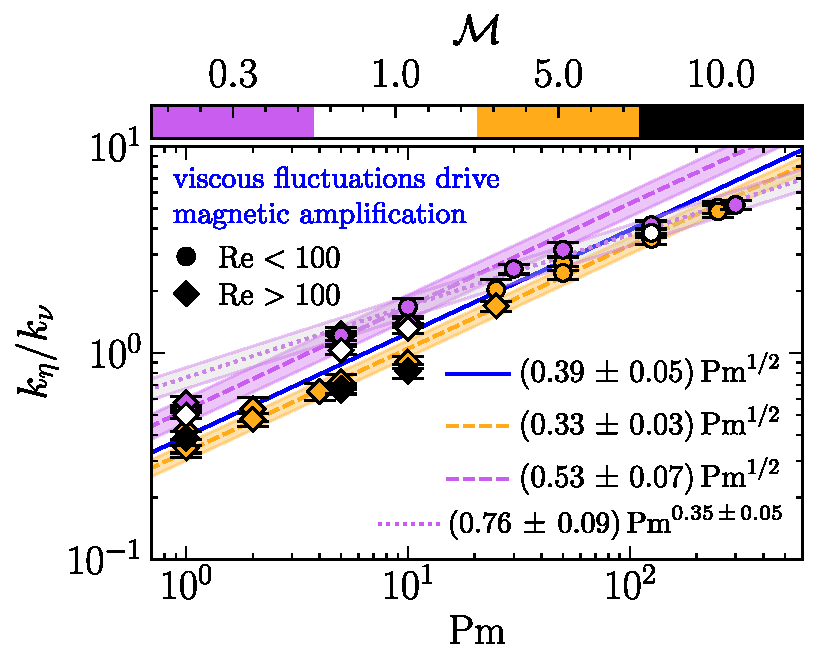
\includegraphics[width=0.49\linewidth]{figures/ssd-exp/scaling_keta_cur_updated.pdf}
    \caption{\DIFaddFL{In the left panel we plot the scale separation between the converged kinetic dissipation wavenumber ($k_\nu$) and the external forcing wavenumber ($k_\mathrm{turb} = 2$) as a function of the hydrodynamic Reynolds number ($\mReh$) for each simulation setup in }\autoref{table:ssd-exp:summary}\DIFaddFL{. In the right panel we also compare the scale separation between the converged magnetic and kinetic dissipation wavenumbers ($k_\eta / k_\nu$) against the magnetic Prandtl number ($\mPrm$). Points are coloured by $\mSonicMach$, where $\mSonicMach = 0.3$ simulations are coloured magenta, $\mSonicMach = 1$ are coloured white, $\mSonicMach = 5$ are coloured yellow, and $\mSonicMach = 10$ are coloured black. To guide the eye in the left panel, we fit theoretical scalings of $k_\nu$ in different flow regimes: $k_\nu \sim \mReh^{2/3}$ to supersonic ($\mSonicMach > 1$) simulations (solid yellow line; expected for \mbox{%DIFAUXCMD
\citealt{burgers1948_turbulence_model} }\hskip0pt%DIFAUXCMD
turbulence), $k_\nu \sim \mReh^{3/4}$ to the turbulent ($\mReh \geq \mReh_\mathrm{crit} \approx 100$) subset of trans- and subsonic ($\mSonicMach \leq 1$) simulations (dashed magenta line; expected for \mbox{%DIFAUXCMD
\citealt{kolmogorov1941dissipation} }\hskip0pt%DIFAUXCMD
turbulence), and $k_\nu \sim \mReh^{3/8}$ to viscous ($\mReh < \mReh_\mathrm{crit}$), trans- and subsonic velocity fields (dotted magenta line; see \mbox{%DIFAUXCMD
\citetalias{kriel2022fundamental}}\hskip0pt%DIFAUXCMD
). In the right panel we plot viscous simulations ($\mReh < \mReh_\mathrm{crit}$) as circles, and turbulent simulations ($\mReh \geq \mReh_\mathrm{crit}$) as diamonds. We also fit a $k_\eta/k_\nu \sim \mPrm^{1/2}$ scaling to the full dataset (solid blue line), the supersonic simulations (dashed yellow line), and the turbulent subset of the trans- and subsonic simulations (dashed magenta line). Finally, we also fit a general power-law model to the viscous subset of trans- and subsonic simulations, and recover a fit (dotted magenta line) that is consistent with our findings in \mbox{%DIFAUXCMD
\citetalias{kriel2022fundamental}}\hskip0pt%DIFAUXCMD
, where the range of subviscous scales has a shallower dependence on $\mPrm$ than in the turbulent regime. We report all fitted parameters and their 1-sigma uncertainties in their respective labels.}}
    \label{fig:dissipation_scaling}
\end{figure}

\DIFaddend \subsection{Where Does Kinetic and Magnetic Energy Dissipate?}
\label{sec:results:dissipation}

Now that we have obtained converged dissipation wavenumbers, we are prepared to explore how these scales depend on the dimensionless plasma parameters $\mSonicMach$, $\mReh$ and $\mPrm$. In the kinematic phase of the dynamo, where magnetic fields are subdominant on all scales, we expect the separation between \DIFdelbegin \DIFdel{$k_0$ }\DIFdelend \DIFaddbegin \DIFadd{$k_\mathrm{turb}$ }\DIFaddend and $k_\nu$ (\ie the inertial range) to depend only on the velocity field properties (\ie $\mReh$), and the separation between $k_\nu$ and $k_\eta$ (\ie the sub-viscous range) to be a function of only $\mPrm$. The exact relationship between these dissipation scales and the principal plasma parameters should change between the subsonic and supersonic regimes, an effect we explore in \autoref{fig:dissipation_scaling}. Here we plot \DIFdelbegin \DIFdel{$k_\nu / k_0$ }\DIFdelend \DIFaddbegin \DIFadd{$k_\nu / k_\mathrm{turb}$ }\DIFaddend against $\mReh$ in the left panel and $k_\eta / k_\nu$ against $\mPrm$ in the right panel, in both cases colour-coding the simulations by $\mSonicMach$.

\subsubsection{Viscous Scaling (Inertial Range)}
\label{sec:results:dissipation:knu}

We first consider the scaling behaviour of $k_\nu$, and its dependence on $\mReh$ (left hand panel of \autoref{fig:dissipation_scaling}). Here, for our turbulent ($\mReh \gtrsim \mReh_\mathrm{crit}$), subsonic ($\mSonicMach = 0.3$; plotted in yellow) and transsonic ($\mSonicMach = 1$; plotted in white) simulations, we recover \DIFdelbegin \DIFdel{$k_\nu / k_0 \sim \mReh^{3/4}$ }\DIFdelend \DIFaddbegin \DIFadd{$k_\nu / k_\mathrm{turb} \sim \mReh^{3/4}$ }\DIFaddend as expected for \citet{kolmogorov1941dissipation} turbulence where $E_{\mathrm{kin}}(k) \sim k^{-5/3}$. This is the same scaling behaviour we had previously demonstrated in \citetalias{kriel2022fundamental} using our previous methods, and now, here, we confirm that our new method (\autoref{eqn:knu_measure}) recovers the same scaling in the same flow regime. This scaling has also been extensively demonstrated in both numerical simulations \citep{yeung1997universality, schumacher2007sub, schumacher2014small} and laboratory experiments \citep{barenblatt1997scaling}, and reflects the conservation of energy flux through the self-similar, inertial cascade, with dissipation only becoming significant at the viscous scale.

For our viscous ($\mReh < \mReh_\mathrm{crit}$), trans- and subsonic ($\mSonicMach \leq 1$) simulations, we recover \DIFdelbegin \DIFdel{$k_\nu / k_0 \sim \mReh^{3/8} = (\mReh^{3/4})^{1/2}$}\DIFdelend \DIFaddbegin \DIFadd{$k_\nu / k_\mathrm{turb} \sim \mReh^{3/8} = (\mReh^{3/4})^{1/2}$}\DIFaddend . This result again agrees with our previous findings in \citetalias{kriel2022fundamental}, where we had found that viscous, subsonic flows have sub-Gaussian velocity gradients. These gradients reflect a lack of intense, localised dissipation events, characteristic of more stable, laminar-like flow regimes \citep[\eg][]{schumacher2007sub, schumacher2014small}, where energy cascade is less efficient compared with \citet{kolmogorov1941dissipation} turbulence.

Finally, for our supersonic ($\mSonicMach = 5$ and $10$) simulations we measure \DIFdelbegin \DIFdel{$k_\nu / k_0 \sim \mReh^{2/3}$}\DIFdelend \DIFaddbegin \DIFadd{$k_\nu / k_\mathrm{turb} \sim \mReh^{2/3}$}\DIFaddend , which corresponds with \citet{burgers1948_turbulence_model} turbulence where $E_{\mathrm{kin}}(k) \sim k^{-2}$ \citep{schober2012magnetic, Federrath2021_sonic_scale}. This scaling of $k_\nu$ sits intermediate between that expected for \citet{kolmogorov1941dissipation} turbulence and the scaling for a viscous, subsonic velocity field \citepalias{kriel2022fundamental}. It reflects shock-dominated energy transfer, where dissipation occurs on all inertial scales, unlike in \citet{kolmogorov1941dissipation} turbulence, where dissipation only occurs on and below the viscous scale.

\DIFdelbegin %DIFDELCMD < \begin{figure}
%DIFDELCMD <     \centering
%DIFDELCMD <     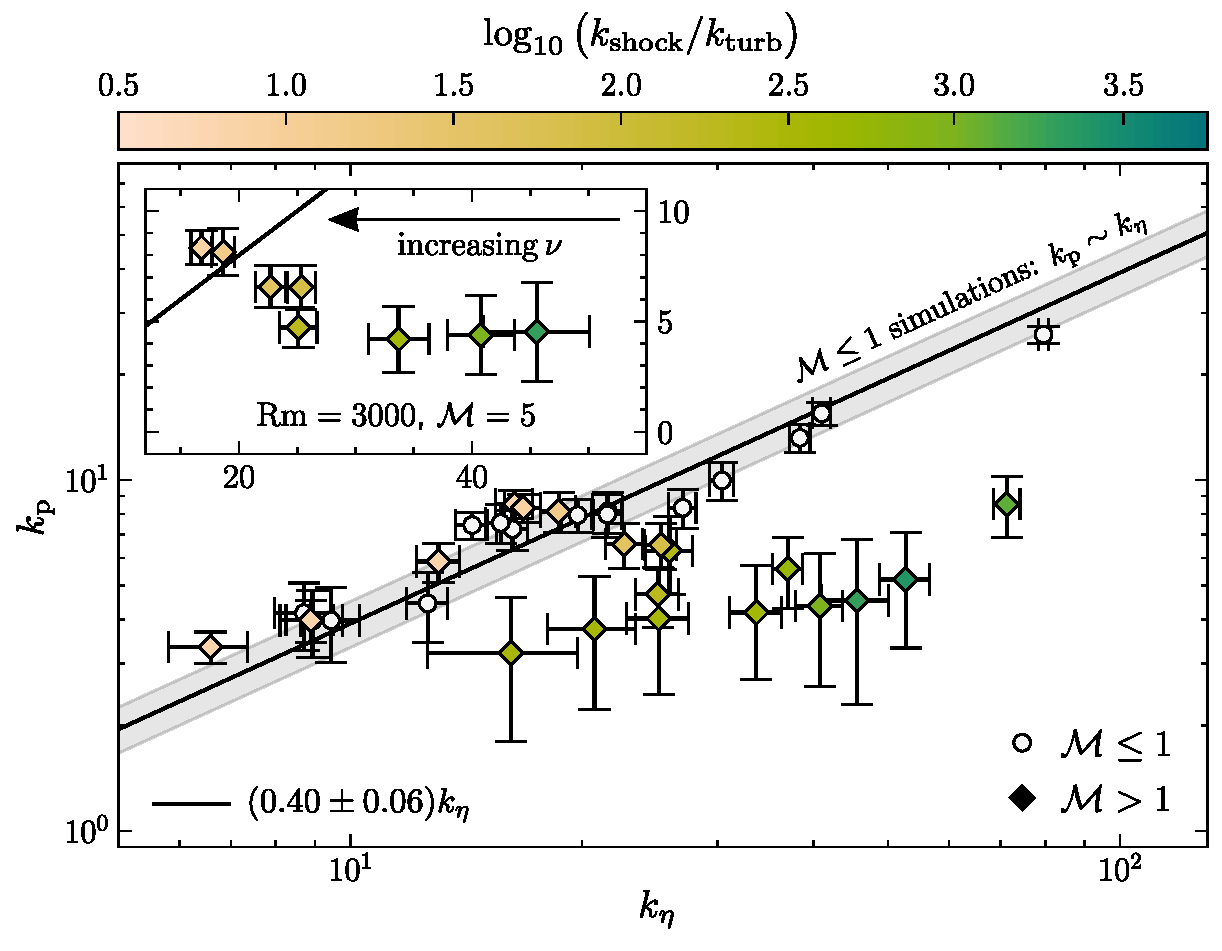
\includegraphics[width=\linewidth]{figures/ssd-exp/scaling_kp.pdf}
%DIFDELCMD <     %%%
%DIFDELCMD < \caption{%
{%DIFAUXCMD
\DIFdelFL{Converged magnetic peak wavenumber ($k_\mathrm{p}$), plotted against the converged characteristic magnetic dissipation wavenumber ($k_\eta$), for each simulation setup in }%DIFDELCMD < \autoref{table:ssd-exp:summary}%%%
\DIFdelFL{. In the main panel, we plot sub- and transsonic simulations with white circles, and in both (main as well as inset) panels, we plot supersonic simulations with diamonds that are coloured based on the reciprocal of our characteristic shock width model ($k_\mathrm{shock}$; see }%DIFDELCMD < \autoref{eqn:shock_width}%%%
\DIFdelFL{). To provide further insights into the supersonic dynamics, we add an inset panel where we focus on a subset of the supersonic simulations. In this inset, we plot the set of $\mSonicMach = 5$ simulations where $\mRem = 3000$ is fixed, and $\mReh$ is changed via $\nu$. In both panels, we also annotate the same $k_\mathrm{p} \sim k_\eta$ fit in black, indicating the 1-sigma standard deviation of $k_\mathrm{p} / k_\eta$ in the $\mSonicMach \leq 1$ subset of points, using a grey coloured band in the main panel.}}
    %DIFAUXCMD
%DIFDELCMD < \label{fig:kp_scaling}
%DIFDELCMD < \end{figure}
%DIFDELCMD <

%DIFDELCMD < %%%
\DIFdelend To summarise these three regimes, we find
\DIFdelbegin %DIFDELCMD < \begin{align}
%DIFDELCMD <     \frac{k_{\nu}}{k_{0}}
%DIFDELCMD <         \sim \left\{\begin{matrix}
%DIFDELCMD <             \mReh^{3/8}, & \mSonicMach \leq 1, & \mReh < \mReh_\mathrm{crit}, \\
%DIFDELCMD <             \mReh^{3/4}, & \mSonicMach \leq 1, & \mReh \geq \mReh_\mathrm{crit}, \\
%DIFDELCMD <             \mReh^{2/3}, & \mSonicMach > 1 .
%DIFDELCMD <         \end{matrix}\right.
%DIFDELCMD <     \label{eqn:knu_scaling}
%DIFDELCMD < \end{align}%%%
\DIFdelend \DIFaddbegin \begin{align}
    \frac{k_{\nu}}{k_\mathrm{turb}}
        \sim \left\{\begin{matrix}
            \mReh^{3/8}, & \mSonicMach \leq 1, & \mReh < \mReh_\mathrm{crit}, \\
            \mReh^{3/4}, & \mSonicMach \leq 1, & \mReh \geq \mReh_\mathrm{crit}, \\
            \mReh^{2/3}, & \mSonicMach > 1 .
        \end{matrix}\right.
    \label{eqn:knu_scaling}
\end{align}\DIFaddend

The fact that during the kinematic phase of our SSD simulations, we have, in all cases, recovered well-known viscous scaling results for purely hydrodynamic turbulence, is not surprising, since during the kinematic phase \mbox{$E_\mathrm{mag}(k) \ll E_\mathrm{kin}(k)$} for all $k$ (see \citealt{beattie2022growth} for the sub-sonic $E_\mathrm{mag}(k)/E_\mathrm{kin}(k)$ functions showing this), and therefore the magnetic field exerts a negligible Lorentz force\footnote{
    \citet{brandenburg2023dissipative}, for example, recognised this simplification and explicitly removed the Lorentz force from the momentum conservation equation, thereby allowing them to indefinitely explore the kinematic SSD phase, as the plasma has no means to become aware of the magnetic field.
}. Thus \autoref{mhd:momentum} becomes independent of $\mVector{b}$, and approximately hydrodynamical. Once $\mVector{b}$ is strong enough (as the SSD process transitions into the nonlinear and saturated phases), we do not expect these dissipation scalings to persist, but measuring these scalings in the other growth regimes is beyond the scope of the current study.

\subsubsection{Resistive Scaling (Sub-Viscous Range)}
\label{sec:results:dissipation:keta}

Next, in the right hand panel of \autoref{fig:dissipation_scaling} we consider the subviscous range of scales ($k_\nu < k < k_\eta)$, and determine how the scale-separation between $k_\eta$ and $k_\nu$ depends upon $\mPrm$. This is the most direct way to test whether, even in supersonic flows, the smallest scale kinetic fluctuations are responsible for amplifying (shearing) magnetic fields (see \S\ref{sec:ICs:Pm} for details). And in fact, we find evidence that the size of the subviscous range of scales is directly proportional to $\mPrm^{1/2}$ in the turbulent, subsonic regime, as well as in the supersonic flow regime. However, as in \citetalias{kriel2022fundamental}, we find that this scaling does not appear to hold in the viscous, trans- and subsonic flow regimes.

Now, perhaps this is not completely unexpected, because the theoretical expectation that $k_\eta \sim k_\nu \,\mPrm^{1/2}$ follows from arguments that do not make any assumption about the underlying flow properties of the velocity field (\ie if the flow is subsonic or supersonic). For example, \citet{schekochihin2002spectra} predicted this scaling by assuming that viscous-scale fluctuations most dominantly amplify the magnetic field, with characteristic shearing (or stretching) rate $u_\nu / \ell_\nu$; where $u_\nu$ is the velocity on scale $\ell_\nu$. Balancing this rate of energy injection (into the magnetic field) with the rate of magnetic (Ohmic) dissipation, $\eta / \ell_\eta^2$, rearranges to give
\begin{align}
    \ell_\eta
        \sim \rbrac{\frac{\eta \, \ell_\nu}{u_\nu}}^{1/2}
        = \rbrac{\ell_\nu^2 \frac{\eta}{\nu} \frac{\nu}{\ell_\nu u_\nu}}^{1/2}
        \sim \ell_\nu \, \mPrm^{-1/2}
    , \label{eqn:keta:result}
\end{align}
where $\ell_\nu \sim \nu / u_\nu$ follows from a straightforward unit analysis.

Here, the key assumption is the existence of a characteristic viscous scale, where shearing occurs fastest, while the fluctuations still carry a significant amount of energy. For simple plasma flows in the kinematic SSD phase, where there is a single turbulent cascade, this corresponds with the smallest scale in the turbulent cascade. At smaller scales, fluctuations may induce shearing on faster timescales, but their energy dissipates to the point where they contribute negligibly to magnetic amplification. The nature of the energy transfer process that leads to the viscous scale is also not important, as long as the concept of a viscous scale -- below which the kinetic energy cascade dissolves -- remains meaningful. Moreover, the relation $\ell_\nu \sim \nu / u_\nu$, derived from dimensional considerations, represents a general balance between viscous forces and inertial effects. Therefore, while the model of \citet{schekochihin2002spectra} draws upon concepts inspired by \citet{kolmogorov1941dissipation}-like turbulence, its applicability also extends beyond, as we have shown, for example, to the supersonic regime.

On this basis, we conclude that \mbox{$k_\eta \sim k_\nu\, \mPrm^{1/2}$} is a universal scaling in the kinematic phase of turbulent ($\mReh \geq \mReh_\mathrm{crit}$), $\mPrm \geq 1$ SSDs, invariant to the presence of shocks (\ie $\mSonicMach$). This result supports the idea that the smallest (viscous) fluctuations are always responsible for converting kinetic into magnetic energy, regardless of whether the kinetic energy cascade follows a \citet{burgers1948_turbulence_model}-like or \citet{kolmogorov1941dissipation}-like behaviour. However, we find that the scale separation between $k_\nu$ and $k_\eta$ is generally larger for subsonic compared with supersonic flows (evidenced by larger fitted coefficients in the right panel of \autoref{fig:dissipation_scaling}). This aligns with previous works which have shown that turbulent, subsonic flows are more efficient at driving SSD growth than their supersonic counterparts, even for plasmas with the same $\mPrm$ \citep{schober2012magnetic}.

\subsection{What Sets the Scale Where Magnetic Energy Peaks?}
\label{sec:results:peak}

\DIFaddbegin \begin{figure}
    \centering
    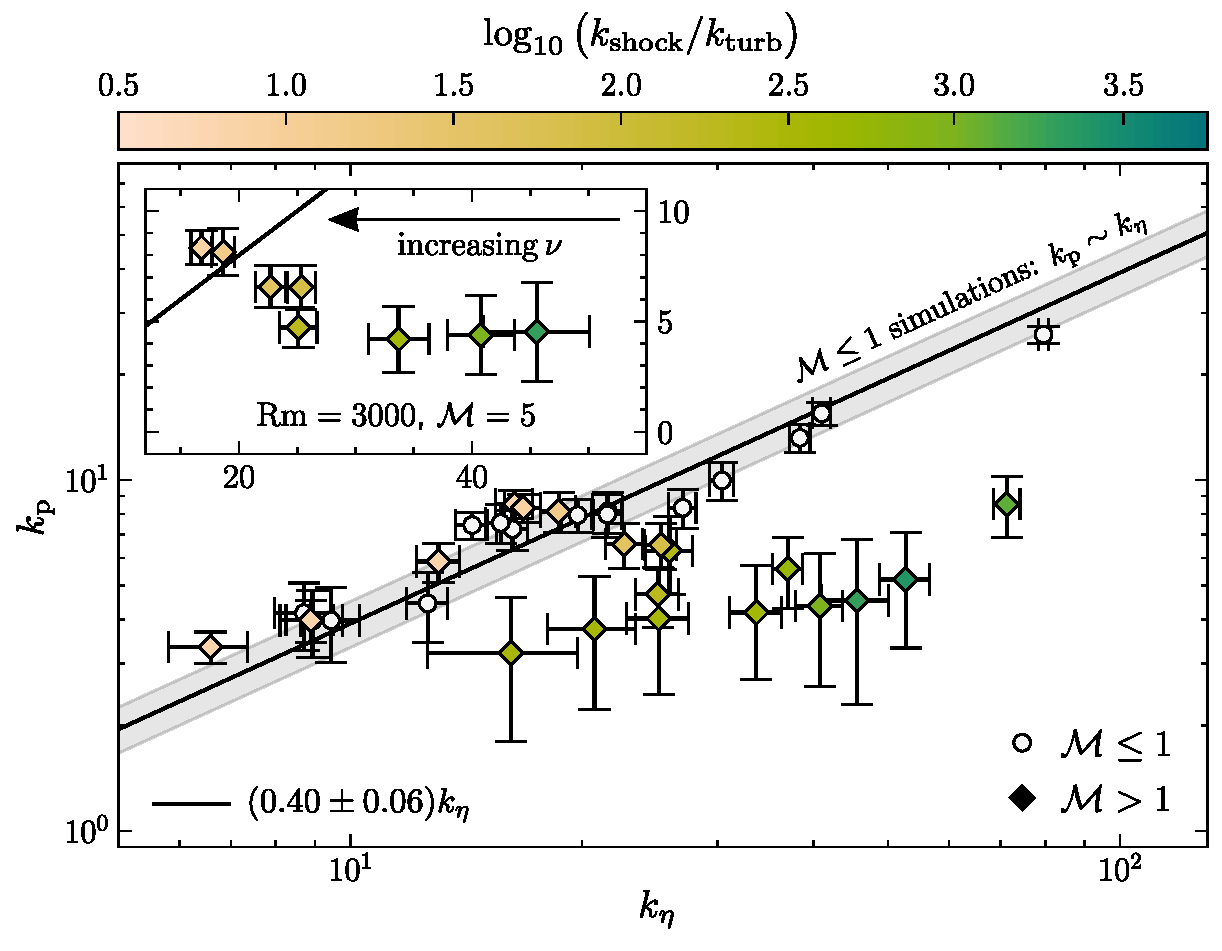
\includegraphics[width=\linewidth]{figures/ssd-exp/scaling_kp.pdf}
    \caption{\DIFaddFL{Converged magnetic peak wavenumber ($k_\mathrm{p}$), plotted against the converged characteristic magnetic dissipation wavenumber ($k_\eta$), for each simulation setup in }\autoref{table:ssd-exp:summary}\DIFaddFL{. In the main panel, we plot sub- and transsonic simulations with white circles, and in both (main as well as inset) panels, we plot supersonic simulations with diamonds that are coloured based on the reciprocal of our characteristic shock width model ($k_\mathrm{shock}$; see }\autoref{eqn:shock_width}\DIFaddFL{). To provide further insights into the supersonic dynamics, we add an inset panel where we focus on a subset of the supersonic simulations. In this inset, we plot the set of $\mSonicMach = 5$ simulations where $\mRem = 3000$ is fixed, and $\mReh$ is changed via $\nu$. In both panels, we also annotate the same $k_\mathrm{p} \sim k_\eta$ fit in black, indicating the 1-sigma standard deviation of $k_\mathrm{p} / k_\eta$ in the $\mSonicMach \leq 1$ subset of points, using a grey coloured band in the main panel.}}
    \label{fig:kp_scaling}
\end{figure}

\DIFaddend In \autoref{fig:kp_scaling} we plot the wavenumber where the magnetic energy spectrum peaks ($k_\mathrm{p}$), and compare it with the characteristic resistive wavenumber ($k_\eta$), for all of our simulations. As in \autoref{fig:field_slices}, we again notice an interesting dichotomy between the subsonic and supersonic simulations, with the scaling of $k_\mathrm{p}$ derived from the $\mSonicMach \leq 1$ (sub- and transsonic) behaving differently to the $\mSonicMach > 1$ (supersonic) simulations. To make this difference between these two flow regimes clear, we introduce a new colouring criteria for all our simulations, one where we colour all the $\mSonicMach \leq 1$ simulations white, and colour the $\mSonicMach > 1$ simulations based on a colour map that we will discuss and motivate below.

Before we move to the supersonic simulations, we again verify that our new methods for measuring $k_\mathrm{p}$ and $k_\eta$ are robust and reliable. To demonstrate this, we highlight that we find $k_\mathrm{p} = (0.40 \pm 0.06)\, k_\eta$, which recovers $k_\mathrm{p} \sim k_\eta$ for our $\mSonicMach \leq 1$ subset of SSD simulations (white points). This is a well known theoretical result \citep[\eg][]{schekochihin2002spectra}, which was confirmed in previous numerical simulations (\DIFaddbegin \DIFadd{\mbox{%DIFAUXCMD
\citealt{schekochihin2004simulations}}\hskip0pt%DIFAUXCMD
; \mbox{%DIFAUXCMD
\citealt{haugen2004simulations}}\hskip0pt%DIFAUXCMD
; }\DIFaddend \citetalias{kriel2022fundamental}; \citealt{brandenburg2023dissipative}), and tells us that in the kinematic phase of (even approximately) incompressible SSDs, magnetic energy becomes concentrated at the smallest scales allowed by magnetic dissipation \citep[\eg][]{schekochihin2002spectra, Xu2016_dynamo, kriel2022fundamental, brandenburg2023dissipative}. Now, notice that the $0.40 \pm 0.06$ constant of proportionality in this relation is dependent upon the models used to measure $k_\mathrm{p}$ and $k_\eta$, and therefore expectantly, it is different from the $1.2 \pm 0.2$ found in \citetalias{kriel2022fundamental} (see \S\ref{sec:results:tools} for a discussion on our choice of new models for $k_\eta$ and $k_\mathrm{p}$).

The behaviour of $k_\mathrm{p}$ for supersonic SSDs during the kinematic phase is dramatically different from the subsonic scaling, though. While a portion of our $\mSonicMach > 1$ simulations follow the same $k_\mathrm{p} \sim k_\eta$ scaling as the subsonic cases, the rest deviate significantly to smaller wavenumbers, \viz $k_\mathrm{p} < k_\eta$. To develop an intuition for why this happens, we briefly turn our attention back to the bottom row panels in \autoref{fig:field_slices}, which show runs \SimName{5}{24}{125}, \SimName{5}{600}{5}, and \SimName{5}{3000}{1}, respectively. In \SimName{5}{3000}{1}, for example, magnetic energy (red) seems to be preferentially concentrated inside of shocked regions of gas, where there are large jumps in the density field (black contours), that have previously been shown to be coherent up to \DIFdelbegin \DIFdel{$k_0$ }\DIFdelend \DIFaddbegin \DIFadd{$k_\mathrm{turb}$ }\DIFaddend (and even beyond, depending upon how strong the magnetic field is;  \citealt{beattie2020filaments,Beattie2021_multi_shock_model}), even though they fill very little of the volume \citep[e.g.,][]{Hopkins2013_s_pdf, Robertson2018_dense_regions, Mocz2019_s_pdf, Beattie2022_spdf}. Based on $k_\mathrm{p}$, shocks do not seem to be present in \SimName{5}{24}{125}, where, even though the velocity dispersion is large (\DIFdelbegin \DIFdel{$u_0 \gtrsim 5 c_\mathrm{s}$}\DIFdelend \DIFaddbegin \DIFadd{$u_\mathrm{turb} \gtrsim 5 c_\mathrm{s}$}\DIFaddend ), the kinetic energy diffusion coefficient, $\nu$, is large enough to dissipate supersonic velocities before they form shocks. A likely criteria for this effect is that the shock lifetime, \DIFdelbegin \DIFdel{$t_\mathrm{shock} \sim \ell/u_0$ }\DIFdelend \DIFaddbegin \DIFadd{$t_\mathrm{shock} \sim \ell/u_\mathrm{turb}$ }\DIFaddend (which is a fraction of the sound crossing time across the shocked region, $\ell/c_s$; \citealt{Robertson2018_dense_regions}), is shorter than the diffusion timescale, $t_\nu \sim \ell_\nu^2 / \nu$. When this condition is met, shocks, which naturally occur at scales larger than the viscous fluctuations, are able to create and sustain large-scale structure in the magnetic field faster than the viscosity diffuses them away, and generates subviscous scale magnetic structure.

\begin{figure}
    \centering
    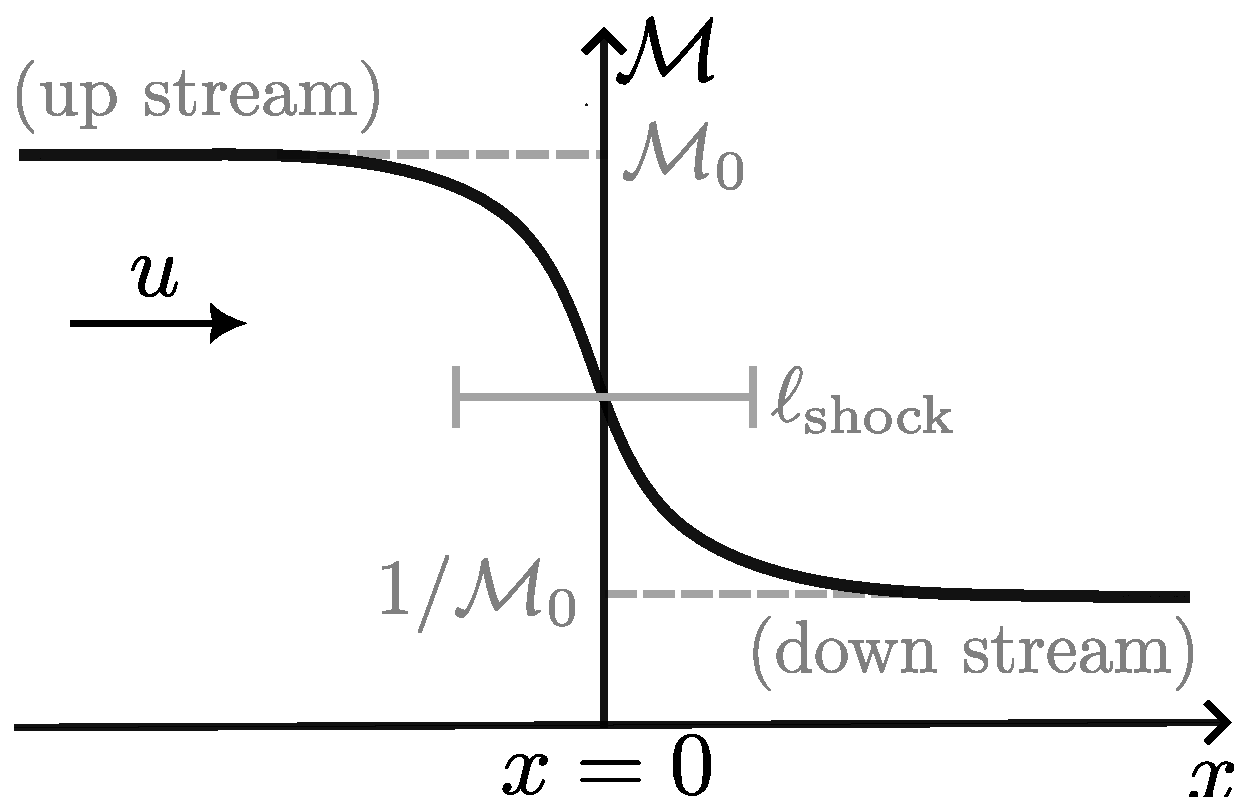
\includegraphics[width=0.5\linewidth]{figures/ssd-exp/schematic_shock.pdf}
    \caption{Schematic of a 1D velocity shock, in the reference frame of the shock: the up stream material ($x < 0$), with up stream sonic Mach number, $\mSonicMach_0$, approaches the shock located at $x = 0$ with a velocity $u$.}
    \label{fig:schematic:1D_shock}
\end{figure}

\subsubsection{The Role of Isotropic Hydrodynamic Shocks}

Our supersonic simulations appear to support a hypothesis that, when shocks are present, $\ell_\mathrm{p}$ approaches a value much larger than $\ell_\eta$, which depends somehow on the typical width of shocks, $\ell_\mathrm{shock}$. To test this conjecture, we estimate $\ell_\mathrm{shock}$ from the quasi-equilibrium state of the momentum equation, omitting the magnetic terms because the Lorentz force is unimportant in the kinematic phase, even in shocked regions ($E_\mathrm{mag}(k)/E_\mathrm{kin}(k) \ll 1,$ for all $k$; \citealt{beattie2022growth}), and excluding external forcing, but not setting viscosity or the sound speed to zero (\eg not going to the pressureless, Burgers' equation limit, $\nabla P/\mSonicMach^2 \to 0$ as $\mSonicMach \to \infty$), namely,
\begin{align}
    \nabla\cdot\rbrac{
            \rho\mVector{u}\otimes\mVector{u}
            + c_\mathrm{s}^2 \rho\mTensor{I}
            - 2\nu\rho\mTensor{V}
        } &= 0 . \label{eqn:momntum:steady_state}
\end{align}
Since shocks are generated isotropically in our supersonic turbulent simulations, we simplify \autoref{eqn:momntum:steady_state} by considering a single characteristic shock travelling in 1D (adopting the usual convention that $x < 0$ and $x > 0$ are the up and down stream directions, respectively; see \autoref{fig:schematic:1D_shock} for a schematic of this setup). It follows that
\begin{align}
    \mddFrac{}{x}\sbrac{
        \rho u^2 + c_\mathrm{s}^2 \rho - \frac{4\nu \rho}{3} \mddFrac{u}{x}
    } = 0 .
    \label{eq:momentum_flux}
\end{align}
The quantity in square brackets represents the momentum flux, which remains constant (conserved) across the shock. Since the velocity gradient vanishes far up stream of the shock, \ie \mbox{$\mdd u/\mdd x \to 0$} as \mbox{$x \to -\infty$}, the momentum flux there must be \DIFdelbegin \DIFdel{$\rho_0 u_0^2 + c_s^2 \rho_0$}\DIFdelend \DIFaddbegin \DIFadd{$\rho_0 u_\mathrm{turb}^2 + c_s^2 \rho_0$}\DIFaddend , where subscript $0$ indicates quantities in the far up stream region. Conservation of mass flux further implies that \DIFdelbegin \DIFdel{$\rho u = \rho_0 u_0 = \mathrm{constant}$}\DIFdelend \DIFaddbegin \DIFadd{$\rho u = \rho_0 u_\mathrm{turb} = \mathrm{constant}$}\DIFaddend , which allows us to write position-dependent quantities (without subscripts), in terms of the upstream values. Making use of these relationships, we integrate \autoref{eq:momentum_flux} and solve for
\begin{align}
    \mddFrac{\mSonicMach}{x}
        = \frac{3 c_\mathrm{s}}{4 \nu} \rbrac{
            \mSonicMach^2 - \rfrac{\mSonicMach_0^2 + 1}{\mSonicMach_0} \mSonicMach + 1
        } ,
        \label{eqn:shock_width:ode}
\end{align}
which captures how $\mSonicMach$ varies across the shocked region.

\begin{figure}
    \centering
    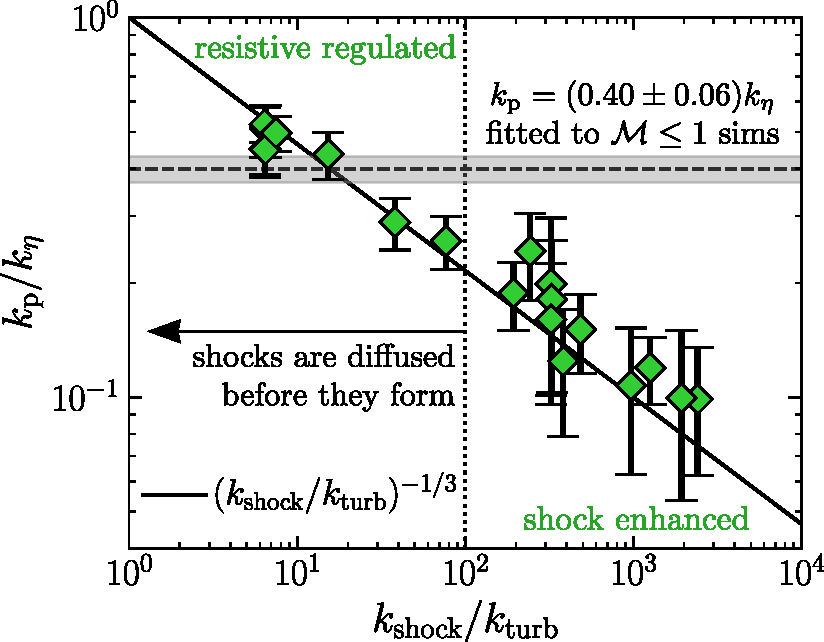
\includegraphics[width=0.65\linewidth]{figures/ssd-exp/scaling_kshock.pdf}
    \caption{For each of our $\mSonicMach > 1$ simulations we compare $k_\mathrm{p}/k_\eta$ with the reciprocal of our model for the shock aspect ratio (\DIFdelbeginFL \DIFdelFL{$k_\mathrm{shock}/k_0$ }\DIFdelendFL \DIFaddbeginFL \DIFaddFL{$k_\mathrm{shock}/k_\mathrm{turb}$ }\DIFaddendFL via \autoref{eqn:shock_width}) plotted as green diamonds. We annotate the scaling relation \DIFdelbeginFL \DIFdelFL{$k_\mathrm{p}/k_\eta = (k_\mathrm{shock}/k_0)^{-1/3}$ }\DIFdelendFL \DIFaddbeginFL \DIFaddFL{$k_\mathrm{p}/k_\eta = (k_\mathrm{shock}/k_\mathrm{turb})^{-1/3}$ }\DIFaddendFL with a solid line, and the measured average $k_\mathrm{p}/k_\eta = 0.40 \pm 0.06$ from the $\mSonicMach \leq 1$ simulations with a dashed line. We also indicate the 1-sigma standard deviation in the $\mSonicMach \leq 1$ subset of $k_\mathrm{p}/k_\eta$ points with a grey band, and annotate \DIFdelbeginFL \DIFdelFL{$k_\mathrm{shock}/k_0 = 10^2$ }\DIFdelendFL \DIFaddbeginFL \DIFaddFL{$k_\mathrm{shock}/k_\mathrm{turb} = 10^2$ }\DIFaddendFL with a vertical dotted line. We find that the scale-separation between $k_\mathrm{p}$ and $k_\eta$ for the supersonic transitions from incompressible (\DIFdelbeginFL \DIFdelFL{$k_\mathrm{shock}/k_0 < 10^2$}\DIFdelendFL \DIFaddbeginFL \DIFaddFL{$k_\mathrm{shock}/k_\mathrm{turb} < 10^2$}\DIFaddendFL ) to compressible (\DIFdelbeginFL \DIFdelFL{$k_\mathrm{shock}/k_0 > 10^2$}\DIFdelendFL \DIFaddbeginFL \DIFaddFL{$k_\mathrm{shock}/k_\mathrm{turb} > 10^2$}\DIFaddendFL ) scaling behaviour when the aspect ratio of filamentary shocks becomes large (captured by \autoref{eqn:shock_width} when $\mSonicMach \gtrsim 1$ and $\mReh \gtrsim \mReh_\mathrm{crit} \approx 100$; \DIFdelbeginFL \DIFdelFL{$k_\mathrm{shock}/k_0 \sim 10^2$}\DIFdelendFL \DIFaddbeginFL \DIFaddFL{$k_\mathrm{shock}/k_\mathrm{turb} \sim 10^2$}\DIFaddendFL ). This is because, in the compressible regime, supersonic flows support and become dominated by shocks, where flux-frozen magnetic fields become compressed by shocks into larger-scale, filamentary structures (see for example the bottom-right panel in \autoref{fig:field_slices}), which brings $k_\mathrm{p}$ from $k_\eta$ towards larger scales (smaller wavenumbers, $k$) by an amount proportional to the reciprocal shock aspect ratio, \DIFdelbeginFL \DIFdelFL{$k_\mathrm{shock}/k_0$ }\DIFdelendFL \DIFaddbeginFL \DIFaddFL{$k_\mathrm{shock}/k_\mathrm{turb}$ }\DIFaddendFL (see \autoref{eqn:shock_width}). Conversely, in the incompressible, supersonic regime, where even though $\mSonicMach > 1$, the flow is so viscous ($\mReh < \mReh_\mathrm{crit}$), that shocks are dissipated before they form (\DIFdelbeginFL \DIFdelFL{$\nu > u_0 \ell_0$}\DIFdelendFL \DIFaddbeginFL \DIFaddFL{$\nu > u_\mathrm{turb} \ell_\mathrm{turb}$}\DIFaddendFL ), and therefore compressed structures do not form, and magnetic energy remains organised in a ``folded field'' configuration (see \S\ref{sec:results:kappa}).}
    \label{fig:kshock_scaling}
\end{figure}

\autoref{eqn:shock_width:ode} has the form of a Riccati equation (nonlinear, quadratic differential equation of first-order) with constant coefficients, and has the solution that $\mdd \mSonicMach/\mdd x = 0$ when $\mSonicMach = \mSonicMach_0$ or $1/\mSonicMach_0$; the former solution represents the up stream region, and the latter the down stream region. Since $x$ does not explicitly appear on the right-hand side of \autoref{eqn:shock_width:ode}, we are free to choose our coordinate system such that $\mSonicMach = 1$ at $x=0$ (as we have done in \autoref{fig:schematic:1D_shock}). From this, we estimate the characteristic shock width as
\DIFdelbegin %DIFDELCMD < \begin{align}
%DIFDELCMD <     \frac{\ell_\mathrm{shock}}{\ell_0}
%DIFDELCMD <         &\sim \frac{1}{\ell_0} \left|
%DIFDELCMD <                 \frac{\mSonicMach}{\mdd\mSonicMach/\mdd x}
%DIFDELCMD <             \right|_{x=0}
%DIFDELCMD <         \sim \frac{\nu}{u_0 \ell_0} \frac{\mSonicMach_0^2}{(\mSonicMach_0 - 1)^2}
%DIFDELCMD <     .
%DIFDELCMD < \end{align}%%%
\DIFdelend \DIFaddbegin \begin{align}
    \frac{\ell_\mathrm{shock}}{\ell_\mathrm{turb}}
        &\sim \frac{1}{\ell_\mathrm{turb}} \left|
                \frac{\mSonicMach}{\mdd\mSonicMach/\mdd x}
            \right|_{x=0}
        \sim \frac{\nu}{u_\mathrm{turb} \ell_\mathrm{turb}} \frac{\mSonicMach_0^2}{(\mSonicMach_0 - 1)^2}
    .
\end{align}\DIFaddend
Now, in supersonic turbulence, one expects to see a population of shocks that take on a wide distribution of $\ell_\mathrm{shock}$ \citep[\eg][]{smith2000distribution, brunt2002interstellar, donzis2012shock, lesaffre2013low, squire2017distribution, Park2019_pops_MHD_shocks, Beattie2020_ansotropic_shocks, Beattie2022_spdf}, where each of the different $\ell_\mathrm{shock}$ are determined by the $\mSonicMach_0$ that is up stream from it. That being said, the distribution of shock widths is regulated by the turbulent properties on \DIFdelbegin \DIFdel{$\ell_0$ }\DIFdelend \DIFaddbegin \DIFadd{$\ell_\mathrm{turb}$ }\DIFaddend \citep{Park2019_pops_MHD_shocks}, where on average, \mbox{$\mSonicMach_0 \approx \mSonicMach$}, and \mbox{\DIFdelbegin \DIFdel{$u_0 \approx u_0$}\DIFdelend \DIFaddbegin \DIFadd{$u_\mathrm{turb} \approx u$}\DIFaddend }. Therefore, we model the characteristic aspect ratio of a shock in our isotropic turbulent simulations as
\DIFdelbegin %DIFDELCMD < \begin{align}
%DIFDELCMD <     \frac{k_0}{k_\mathrm{shock}}
%DIFDELCMD <         = \frac{\ell_\mathrm{shock}}{\ell_0}
%DIFDELCMD <         \sim \frac{\mSonicMach^2}{\mReh\, (\mSonicMach - 1)^2}
%DIFDELCMD <     . \label{eqn:shock_width}
%DIFDELCMD < \end{align}%%%
\DIFdelend \DIFaddbegin \begin{align}
    \frac{k_\mathrm{turb}}{k_\mathrm{shock}}
        = \frac{\ell_\mathrm{shock}}{\ell_\mathrm{turb}}
        \sim \frac{\mSonicMach^2}{\mReh\, (\mSonicMach - 1)^2}
    . \label{eqn:shock_width}
\end{align}\DIFaddend

In the inset axis of \autoref{fig:kp_scaling} we test whether this shock aspect ratio model can explain the difference between $k_\mathrm{p}$ and $k_\eta$ (note that we colour points by the reciprocal of \autoref{eqn:shock_width}, to emphasise that in our experiments, the numerator, $k_\mathrm{shock}$, is changing, and \DIFdelbegin \DIFdel{$k_0 = 2$ }\DIFdelend \DIFaddbegin \DIFadd{$k_\mathrm{turb} = 2$ }\DIFaddend remains fixed in the denominator). Here we plot the full set of $\mSonicMach = 5$ and $\mRem = 3000$ simulations. Within this collection of runs, $\mReh$ is varied via changing $\nu$ (\ie \DIFdelbegin \DIFdel{$u_0$ and $k_0$ }\DIFdelend \DIFaddbegin \DIFadd{$u_\mathrm{turb}$ and $k_\mathrm{turb}$ }\DIFaddend are fixed), and we find that the most turbulent simulation in this set, \SimName{5}{3000}{1}, lies farthest from the $k_\mathrm{p} \sim k_\eta$ relation, while the most viscous simulation, \SimName{5}{24}{125}, lies on the relation. Between these two limits, the inverse shock width (\autoref{eqn:shock_width}) scales directly proportional to the deviation of each point from the $k_\mathrm{p} \sim k_\eta$ relation.

We demonstrate this more explicitly in \autoref{fig:kshock_scaling}, which shows $k_\mathrm{p}/k_\eta$ as a function of \DIFdelbegin \DIFdel{$k_\mathrm{shock}/k_0$}\DIFdelend \DIFaddbegin \DIFadd{$k_\mathrm{shock}/k_\mathrm{turb}$}\DIFaddend , and here it is clear that all the $\mSonicMach > 1$ simulations (green diamond points) are well-fit by the empirical relationship
\DIFdelbegin %DIFDELCMD < \begin{align}
%DIFDELCMD <     \frac{k_\mathrm{p}}{k_\eta}
%DIFDELCMD <         = \rfrac{k_\mathrm{shock}}{k_0}^{-1/3}
%DIFDELCMD <     . \label{eqn:kp_scaling}
%DIFDELCMD < \end{align}%%%
\DIFdelend \DIFaddbegin \begin{align}
    \frac{k_\mathrm{p}}{k_\eta}
        = \rfrac{k_\mathrm{shock}}{k_\mathrm{turb}}^{-1/3}
    . \label{eqn:kp_scaling}
\end{align}\DIFaddend
We interpret this to mean that shocks compress flux-frozen magnetic fields into filamentary structures, bringing $k_\mathrm{p}$ from $k_\eta$ towards larger scales by an amount determined by the aspect ratio of typical shocks, \ie the ratio of shock length (\DIFdelbegin \DIFdel{$\ell_0$}\DIFdelend \DIFaddbegin \DIFadd{$\ell_\mathrm{turb}$}\DIFaddend ), compared with shock width ($\ell_\mathrm{shock}$).

Now, while compressions of flux-frozen magnetic fields do not yield irreversible growth in the magnetic field (see, for example, the top panel of Figure 7 in \citealt{beattie2023bulk}; because growth due to compression is soon negated by dilation), we do see that the compressions introduce qualitatively different and lasting imprints on the field amplitude structure (see, for example, the bottom row panels in \autoref{fig:field_slices}). Because the forcing modes in all of our simulations are \DIFdelbegin \DIFdel{$\ell_0 = \ell_\mathrm{box}/2$}\DIFdelend \DIFaddbegin \DIFadd{$\ell_\mathrm{turb} = \ell_\mathrm{box}/2$}\DIFaddend , the aspect ratio of the shocks, \ie \DIFdelbegin \DIFdel{$\ell_\mathrm{shock}/\ell_0$}\DIFdelend \DIFaddbegin \DIFadd{$\ell_\mathrm{shock}/\ell_\mathrm{turb}$}\DIFaddend , can only change via the shock width, which is mediated by the properties of the medium (\ie $\nu$) and flow ($\mReh$ and $\mSonicMach$). The exact nature in which the aspect ratio of shocks, and thereafter, the scale on which magnetic energy becomes concentrated, depends on fundamental plasma numbers, is well captured by \autoref{eqn:shock_width} and \autoref{eqn:kp_scaling}, respectively\footnote{
    We hypothesise that the exponent $1/3$ in \autoref{eqn:kp_scaling} is likely associated with shocks concentrating magnetic energy into filamentary structures \citep{das2024magnetic}. Therefore, the slope of the $\ell_\mathrm{p}/\ell_\eta$ scaling reflects how magnetic energy is distributed within the plasma, and would likely differ if the shocked regions were not filamentary, but, for example, sheet-like instead.
}.

Moreover, in \autoref{fig:kshock_scaling} we once again see evidence for a critical hydrodynamic Reynolds number $\mReh_\mathrm{crit} \approx 100$ that separates the $\mSonicMach > 1$ flows that are able to support shocks ($\mReh \geq \mReh_\mathrm{crit}$), from those flows where strong viscosity prevents shocks from forming ($\mReh < \mReh_\mathrm{crit}$). This becomes clear in the high $\mSonicMach$ limit, where \mbox{\DIFdelbegin \DIFdel{$k_\mathrm{shock}/k_0 \to \mReh$}\DIFdelend \DIFaddbegin \DIFadd{$k_\mathrm{shock}/k_\mathrm{turb} \to \mReh$}\DIFaddend }, and thus $\mReh = \mReh_\mathrm{crit} \approx 100$ corresponds with \DIFdelbegin \DIFdel{$k_\mathrm{shock}/k_0 \approx 100$}\DIFdelend \DIFaddbegin \DIFadd{$k_\mathrm{shock}/k_\mathrm{turb} \approx 100$}\DIFaddend ; we highlight this value with a dotted vertical line in \autoref{fig:kshock_scaling}. It is clear from the figure that this line roughly identifies where the $\mSonicMach > 1$ simulations transition from $k_\mathrm{p}/k_\eta \approx \mathrm{constant}$ to \DIFdelbegin \DIFdel{$k_\mathrm{p}/k_\eta = (k_\mathrm{shock}/k_0)^{-1/3}$}\DIFdelend \DIFaddbegin \DIFadd{$k_\mathrm{p}/k_\eta = (k_\mathrm{shock}/k_\mathrm{turb})^{-1/3}$}\DIFaddend . Indeed, one should notice that the seven red points that lie to the left of the vertical line in \autoref{fig:kshock_scaling} correspond with the seven that lie along the $k_\mathrm{p} \sim k_\eta$ relation in \autoref{fig:kp_scaling}, where in all seven cases $\mReh < 100$.

\begin{figure}
    \centering
    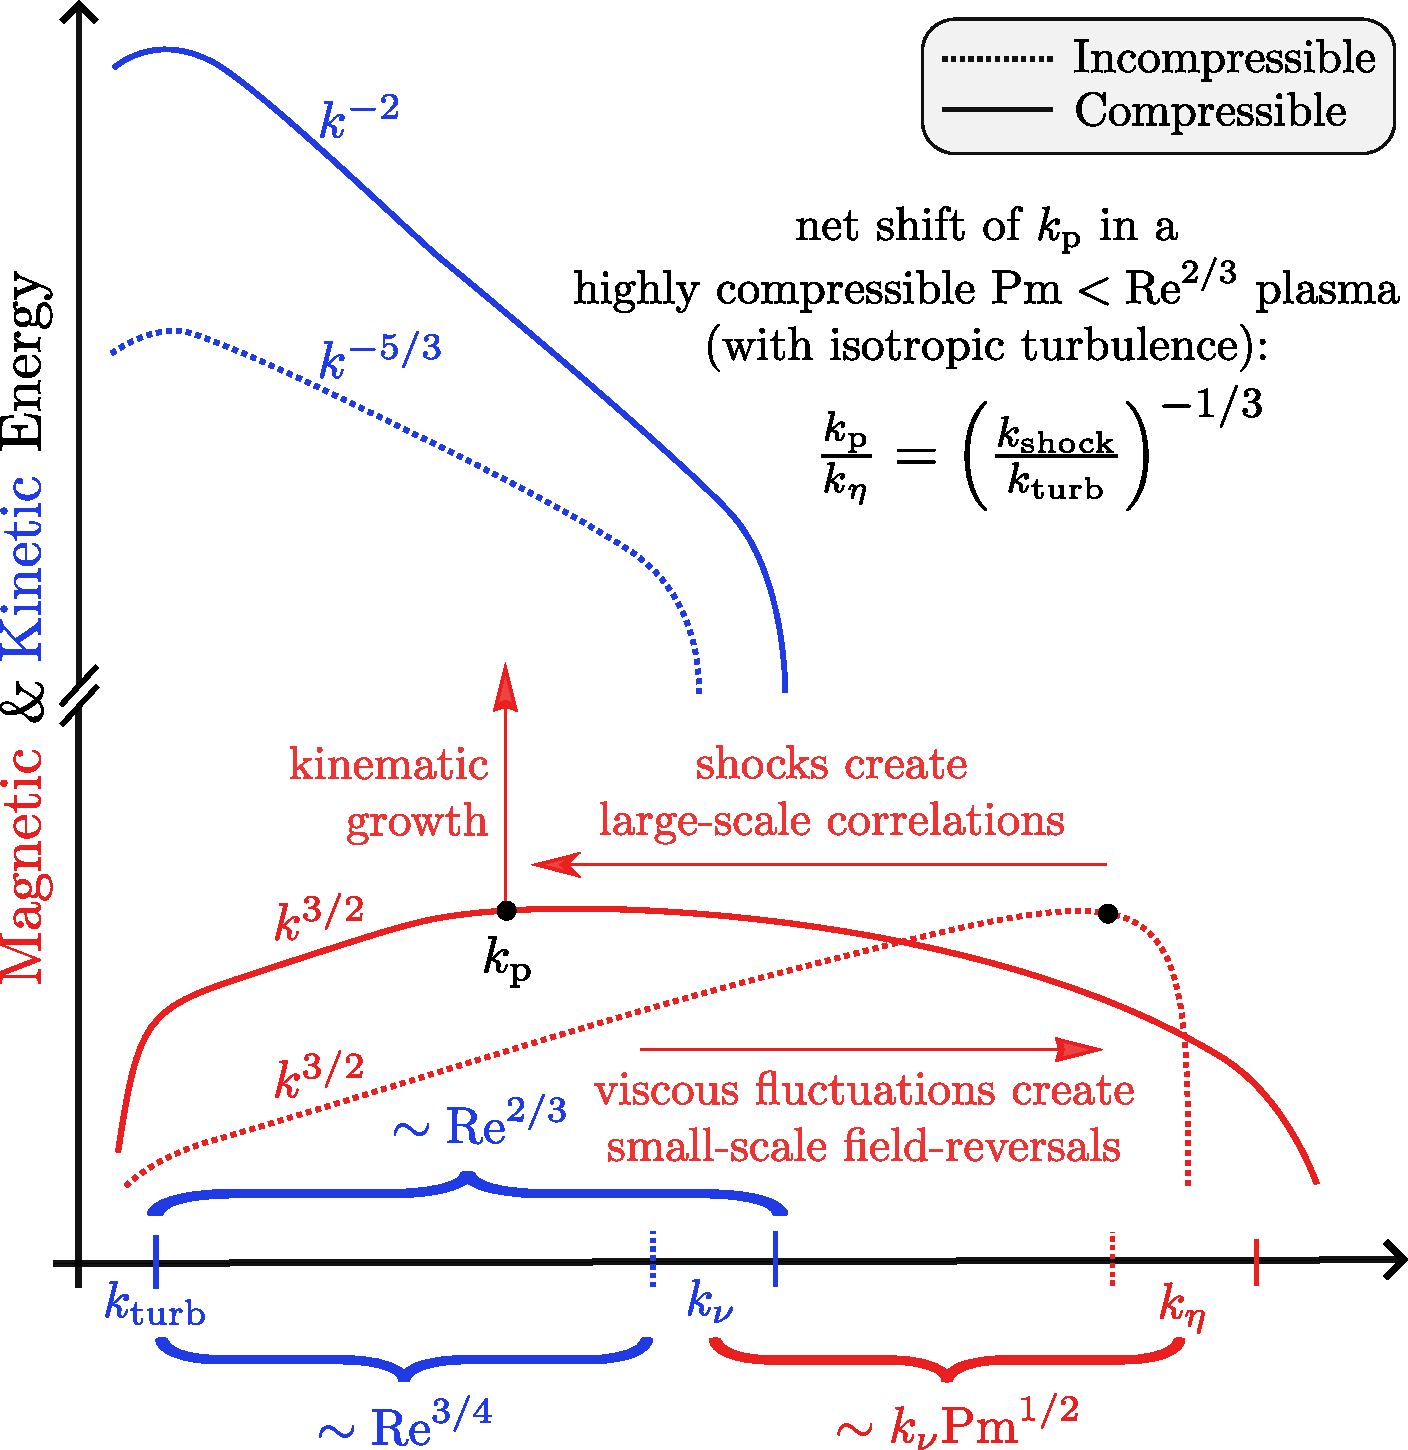
\includegraphics[width=0.8\linewidth]{figures/ssd-exp/schematic_spectra.pdf}
    \caption{Schematic of the important scaling properties of the kinetic (blue) and magnetic (red) energy spectra during the kinematic phase of a turbulent SSD. We summarise our main findings in \autoref{fig:dissipation_scaling} and \ref{fig:kshock_scaling} for incompressible (dotted line) and highly compressible ($\mSonicMach \to \infty$; solid line) plasmas with the same dimensionless plasma parameters $\mReh \geq \mReh_\mathrm{crit}$ and $1 \leq \mPrm < \mReh^{2/3}$. Here we highlight a compressible plasma where the subviscous range is smaller than the net shift in $k_\mathrm{p}$ ($\mPrm < \mReh^{2/3}$), and thus the magnetic tug-of-war between shocks and viscous-scale fluctuations shifts $k_\mathrm{p}$ from $k_\eta$ to beyond $k_\nu$.}
    \label{fig:schematic:energy_spectrum}
\end{figure}

\subsubsection{A Hierarchy of MHD Scales}

We conclude that \autoref{fig:kp_scaling} and \autoref{fig:kshock_scaling} can be explained simply by two distinct flow regimes (see \autoref{fig:schematic:energy_spectrum}). In the first, \textit{incompressible} regime, the development of shocks is not supported by the plasma, whether it is because the velocity dispersion is too small ($\mSonicMach \leq 1$) or because the viscosity is large enough to dissipate the supersonic velocities before shocks are able to form (\ie $\mSonicMach > 1$ and $\mReh < \mReh_\mathrm{crit}$). This results in the well-known hierarchy
\DIFdelbegin %DIFDELCMD < \begin{align}
%DIFDELCMD <    \ell_0 > \ell_\nu > \ell_\eta \sim \ell_\mathrm{p}
%DIFDELCMD <    . \label{eqn:kp:subsonic}
%DIFDELCMD < \end{align}%%%
\DIFdelend \DIFaddbegin \begin{align}
   \ell_\mathrm{turb} > \ell_\nu > \ell_\eta \sim \ell_\mathrm{p}
   . \label{eqn:kp:subsonic}
\end{align}\DIFaddend
In the second, \textit{compressible} (shock-dominated; $\mSonicMach > 1$ and $\mReh \geq \mReh_\mathrm{crit}$) flow regime, shocks concentrate magnetic energy in large-scale, filamentary structures. As a result, the peak magnetic field scale shifts from the resistive scale to \DIFdelbegin \DIFdel{$\ell_\mathrm{p} \sim (\ell_0/\ell_\mathrm{shock})^{1/3} \ell_\eta \gg \ell_\eta$}\DIFdelend \DIFaddbegin \DIFadd{$\ell_\mathrm{p} \sim (\ell_\mathrm{turb}/\ell_\mathrm{shock})^{1/3} \ell_\eta \gg \ell_\eta$}\DIFaddend , approaching $\ell_\mathrm{p} \sim \mReh^{1/3} \ell_\eta$ as \mbox{$\mSonicMach \to \infty$}.

A key question then becomes whether magnetic structures can grow larger than the viscous scale, since scales smaller than $\ell_\nu$ (the subviscous range) are generally on relatively small scales (but not always, e.g., the intracluster medium, with low $\mReh \sim 10^2 \iff k_\nu^{-1} \sim 3\;\mathrm{kpc}$ and extremely high $\mPrm \gtrsim 10^{29}$; \citealt{Schekochihin2006_ICM,StOnge2020_weakly_collisional_dynamo}). Our analysis shows that this can occur, but only when the subviscous range is not too large. To be precise, in the $\mSonicMach \to \infty$ limit, our results (\autoref{eqn:kp_scaling}) indicate that the scale separation between the peak magnetic energy and viscous scales is $\ell_\mathrm{p}/\ell_\nu \sim \mReh^{1/3} \mPrm^{1/2}$, and therefore $\ell_\mathrm{p} > \ell_\nu$ when $\mPrm < \mReh^{2/3}$. This yields the following hierarchy of scales
\DIFdelbegin %DIFDELCMD < \begin{align}
%DIFDELCMD <     \ell_0 > \ell_\mathrm{p} > \ell_\mathrm{shock} > \ell_\nu > \ell_\eta
%DIFDELCMD <     , \label{eqn:kp:supersonic}
%DIFDELCMD < \end{align}%%%
\DIFdelend \DIFaddbegin \begin{align}
    \ell_\mathrm{turb} > \ell_\mathrm{p} > \ell_\mathrm{shock} > \ell_\nu > \ell_\eta
    , \label{eqn:kp:supersonic}
\end{align}\DIFaddend
which we contrast in \autoref{fig:schematic:energy_spectrum} with the hierarchy of scales produced by an incompressible SSD. On the other hand, if $\mPrm > \mReh^{2/3}$ then $\ell_\mathrm{p}$ still shifts from $\ell_\eta$ toward larger scales, but it remains contained in the subviscous range, producing
\DIFdelbegin %DIFDELCMD < \begin{align}
%DIFDELCMD <     \ell_0 > \ell_\nu > \ell_\mathrm{p} > \ell_\mathrm{shock} > \ell_\eta
%DIFDELCMD <     .
%DIFDELCMD < \end{align}%%%
\DIFdelend \DIFaddbegin \begin{align}
    \ell_\mathrm{turb} > \ell_\nu > \ell_\mathrm{p} > \ell_\mathrm{shock} > \ell_\eta
    .
\end{align}\DIFaddend

Here we have shown that shocks in compressible (\mbox{$\mReh \geq \mReh_\mathrm{crit}$} and $\mSonicMach > 1$) flow regimes are able to move the magnetic peak scale out of the subviscous range when $1 \leq \mPrm < \mReh^{2/3}$. Physically, this condition can be understood as a statement that shock lifetimes are longer than the characteristic timescale associated with kinetic fluctuations at the viscous scale (follows from comparing $\ell_\nu/\ell_\eta$ given by \autoref{eqn:keta:result} and $\ell_\mathrm{p}/\ell_\eta$ given by \autoref{eqn:kp_scaling}). If this condition is met, then large scale correlations in the magnetic field are produced through flux freezing in shocks faster than by kinetic amplification on the viscous scale, the mechanism that dominates in all incompressible SSDs. This distinction has important implications for the transition to the saturated regime, which we discuss in \S\ref{sec:discussion:saturation}.

\subsection{Underlying Field Structure}
\label{sec:results:kappa}

\begin{figure}
    \centering
    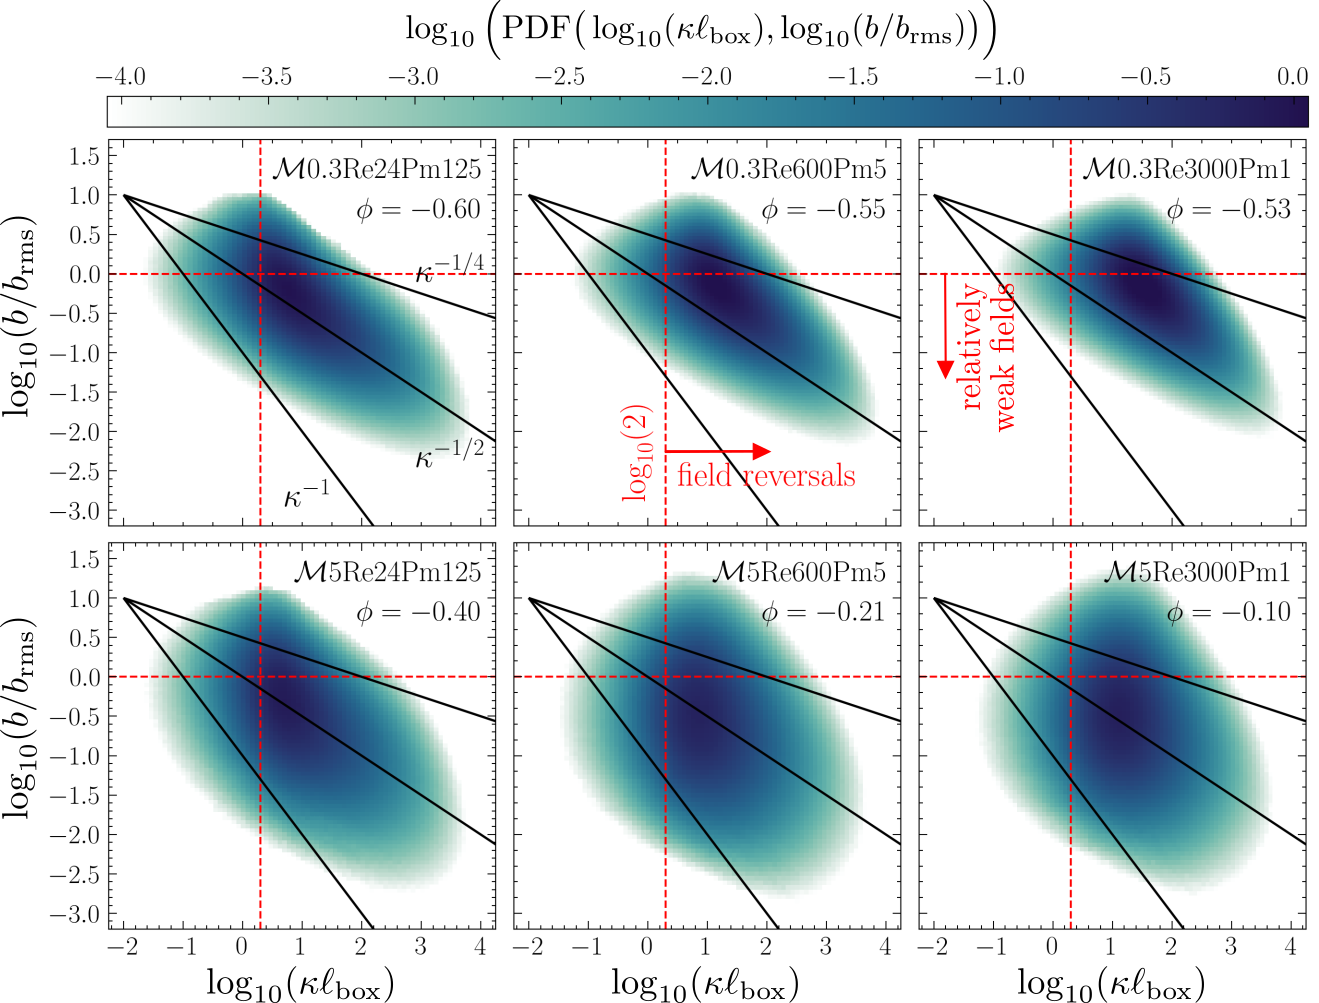
\includegraphics[width=\linewidth]{figures/ssd-exp/2D_jpdfs.png}
    \caption{Joint distributions of the relative magnetic field strength ($b/b_\mathrm{rms}$), and the magnetic field-line curvature ($\kappa$; measured in units of inverse box-length, $\ell_{\mathrm{box}}$), for the same six simulations as in \autoref{fig:field_slices}. In all panels we report the Pearson correlation coefficient $\phi$ (given by \autoref{eq:pearson_correlation}) between $\log_{10}(b/b_\mathrm{rms})$ and $\log_{10}(\kappa/\kappa_\mathrm{rms})$. We also annotate a $b \sim \kappa^{-1/2}$ scaling, which is associated with a curvature relation where the magnetic tension is exactly balanced by the turbulent stretching (the symmetric rate of shear component in $\nabla\otimes\mVector{u}$; \citealt{schekochihin2001structure, schekochihin2004simulations}); see \S\ref{sec:results:kappa} for a discussion. We also show $b \sim \kappa^{-1/4}$ and $b \sim \kappa^{-1}$ to guide the eye. The red, horizontal, dashed lines indicates $b = b_\mathrm{rms}$, while the red, vertical, dashed lines indicate $\kappa \ell_\mathrm{box} = 2$, which marks the transition between fields that can ($\kappa \ell_\mathrm{box} \geq 2$) and cannot ($\kappa \ell_\mathrm{box} < 2$) reverse within the box-domain. The $b\sim \kappa^{-1/2}$ scaling holds well (on average) for the subsonic plasmas (top row), but breaks down for the supersonic plasmas (bottom two right panels), which is most likely due to the presence of shocks being able to compress and grow the field without necessarily modifying the curvature.}
    \label{fig:curvature}
\end{figure}

\begin{figure}
    \centering
    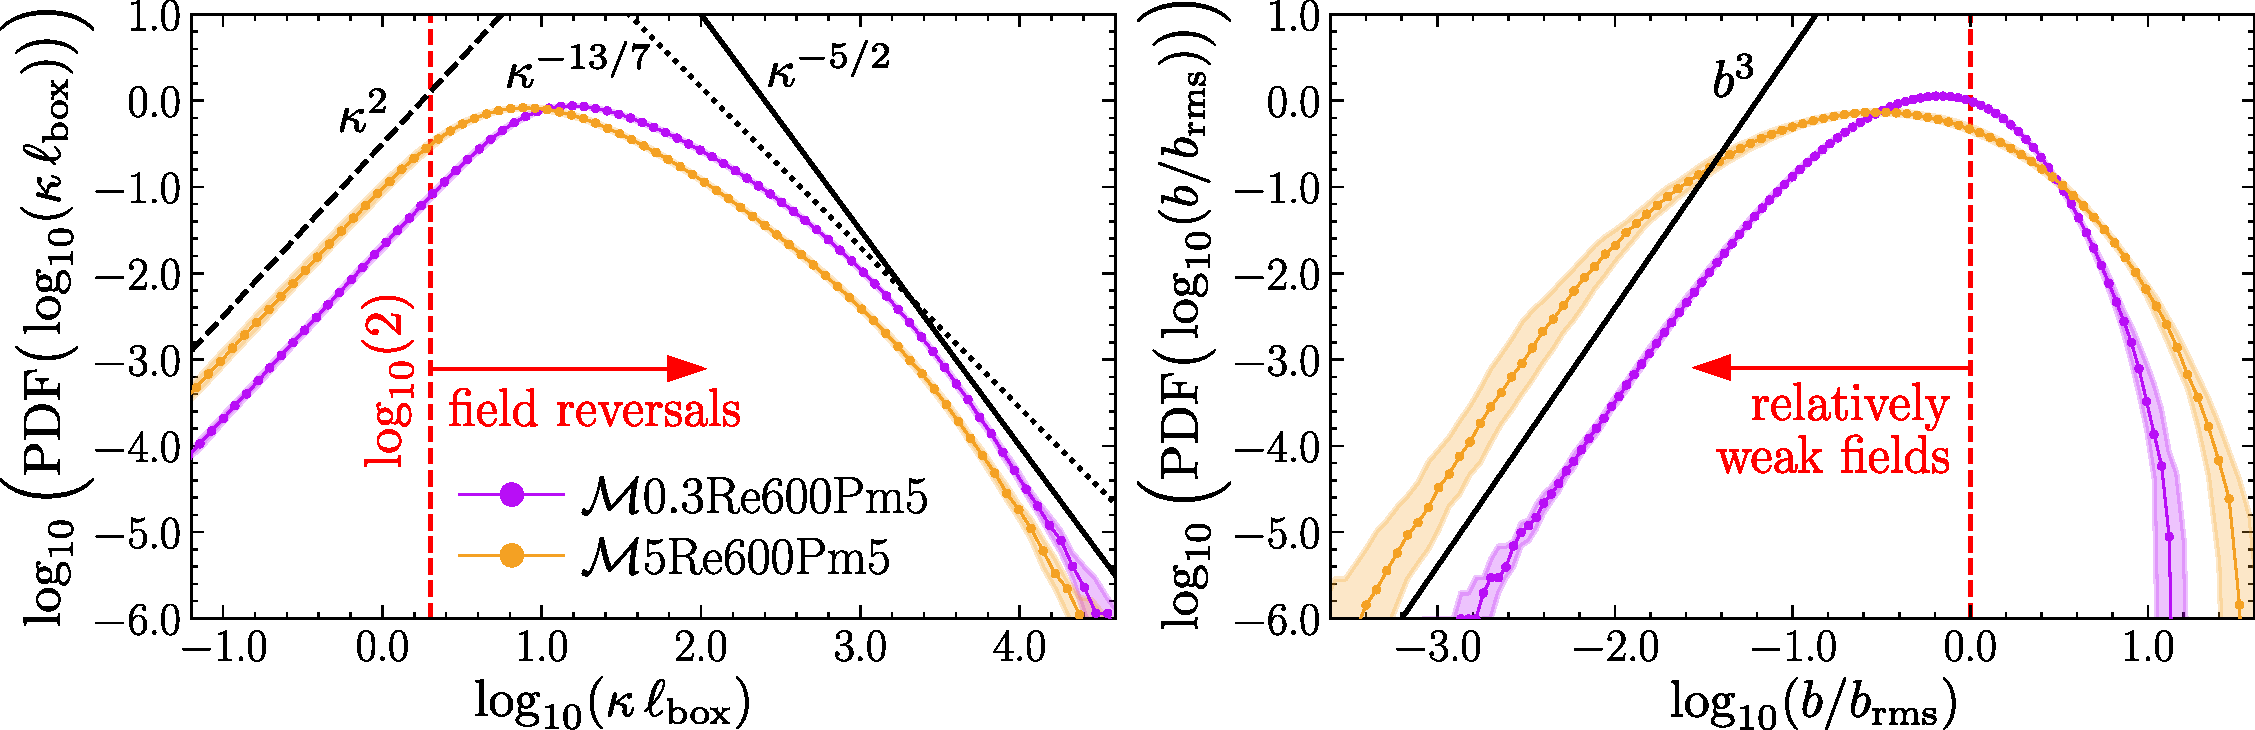
\includegraphics[width=\linewidth]{figures/ssd-exp/1D_pdfs.pdf}
    \caption{Volume-weighted PDFs of the magnetic field-line curvature ($\kappa$, measured in units of $\ell_\mathrm{box}$; left panel), and the normalised magnetic field amplitude ($b/b_\mathrm{rms}$; right panel), for \SimName{0.3}{600}{5} and \SimName{5}{600}{5}. We annotate $\kappa^2$ (dotted), $\kappa^{-13/7}$ (solid; \citealt{schekochihin2002small}), and $\kappa^{-5/2}$ (dash-dotted; \citealt{yang2019role} and \citealt{pfrommer2022simulating}) in the left panel, and $b^{3}$ in the right panel. We only find a negligible difference between the PDFs of $\log_{10}(\kappa \ell_{\mathrm{box}})$ for the $\mSonicMach < 1$ (purple) and $\mSonicMach > 1$ (yellow) simulations, but there is significantly more low and high $b/b_\mathrm{rms}$ probability densities in the $\mSonicMach > 1$ simulation. Hence we conclude that the weakening correlation between $\kappa$ and $b$ (shown in \autoref{fig:curvature}) is caused from shock compressions that grow and shrink $b$ without influencing $\kappa$.}
    \label{fig:pdfs}
\end{figure}

While we have shown that shocks reorganise and concentrate magnetic energy into large-scale, filamentary structures, here we want to show that, in doing so, they also completely change the underlying magnetic field-line properties. To quantify field geometry, we compute the curvature of magnetic field-lines,
\begin{align}
    \kappa
        = \nbrac{ \rbrac{\mVectorBase{t}\cdot\nabla}\mVectorBase{t} }
        , \label{eqn:kappa}
\end{align}
at every point in a simulation domain, where $\mVectorBase{t} = \mVector{b}/\|\mVector{b}\|$ is the tangent vector to the field\footnote{
    Note that in regions where the field changes substantially over the scale of a single cell, as it does in shocked regions, numerical evaluation of $\kappa$ requires some care in choosing a stencil that maintains exact orthogonality of the tangent-normal-binormal basis vectors. See \S\ref{app:kappa} for a discussion of our method, and \citet{schekochihin2004simulations} for a brief acknowledgement of this issue.
}, and curvature points in the $\mVectorBase{n} = (\mVectorBase{t}\cdot\nabla)\mVectorBase{t} / \kappa$ direction. Note that the radius of curvature of the field in units of box length is then $\ell_\mathrm{box}/\kappa$.

\subsubsection{Relationship Between Magnetic Field Strength and Field-Line Curvature}

In \autoref{fig:curvature} we plot the time-averaged, joint distributions of the relative magnetic field strength, $b/b_\mathrm{rms}$ (normalising out the dynamo growth in $b$), and the field-line curvature magnitude, $\kappa \ell_\mathrm{box}$, for the same six simulations as in \autoref{fig:field_slices}, namely \SimName{0.3}{24}{125}, \SimName{0.3}{600}{5}, and \SimName{0.3}{3000}{1} in the top row, and \SimName{5}{24}{125}, \SimName{5}{600}{5}, and \SimName{5}{3000}{1} in the bottom row, respectively. Focusing first, only on the three subsonic simulations (top row of \autoref{fig:curvature}), we find that the $(\kappa,b)$ distributions in both the viscous (left panel) and turbulent SSDs (middle and right panels) appear to have the same overall shape, where the weakest magnetic fields have the largest curvature, \eg have the most field reversals, and conversely the strongest fields are the straightest. Here we find evidence of a scaling consistent with $b \sim \kappa^{-1/2}$, which was first demonstrated by \citet{schekochihin2004simulations} (as opposed to $b \sim \kappa^{-1}$ as previously suggested by \citealt{brandenburg1995size} and \citealt{schekochihin2002small}) for incompressible SSDs, and more recently by \citet{kempski2023cosmic} using $\mSonicMach < 1$ SSD and weak mean-field simulations to study cosmic ray propagation.

\citet{schekochihin2004simulations} associates the $b \sim \kappa^{-1/2}$ anti-correlation with a ``folded field'' geometry\footnote{
    A term coined by \citet{schekochihin2004simulations} to describe the configuration of magnetic fields in the incompressible flow regime.
}, where the incompressible components of the velocity gradient tensor \citep[see][]{beattie2023bulk} and the magnetic tension are balanced. This $1/2$ exponent is a unique solution that produces a steady-state $(\kappa, b)$ configuration in the co-moving frame of the fluid, based on the cancellation of the $\widehat{\mVector{b}}\otimes\widehat{\mVector{b}}:\nabla\mVector{u}$ term in the co-moving, evolution equation for the correlation between the magnetic field amplitude and magnitude of the magnetic field-line curvature (see Equation 25 in \citealt{schekochihin2004simulations}).

In contrast, the supersonic SSDs (bottom row of \autoref{fig:curvature}), show a significantly weaker relationship between the field strength and field-line curvature, with the relative statistical independence of $b$ and $\kappa$ increasing as we evolve from the most viscous plasmas (bottom-left panel) to the most turbulent (bottom-right panel). In the turbulent, supersonic flow regime, it is clear that both strong ($b > b_\mathrm{rms}$) and weak ($b < b_\mathrm{rms}$) field-lines can maintain a straight configuration ($\kappa \ell_\mathrm{box} < 2$), although we still see a dearth of low curvature ($\kappa \ell_\mathrm{box} < 2$) for strong magnetic fields ($b > b_\mathrm{rms}$; \ie the upper left quadrant of the plot is empty). We quantify this growing independence between $b$ and $\kappa$ for each of our simulations in \autoref{fig:curvature} by computing the Pearson correlation coefficient between $\log_{10}(b/b_{\mathrm{rms}})$ and $\log_{10}(\kappa)$,
\begin{align}\label{eq:pearson_correlation}
    \phi = \frac{
            \mathrm{cov}\big[ \log_{10}(b/b_{\mathrm{rms}}) \log_{10}(\kappa\ell_{\mathrm{box}}) \big]
        }{
            \sqrt{
                \mathrm{var}\big[ \log_{10}(b/b_{\mathrm{rms}}) \big]
                \, \mathrm{var}\big[ \log_{10}(\kappa\ell_{\mathrm{box}}) \big]
            }
        }
        ,
\end{align}
where $\mathrm{cov}[\hdots]$ and $\mathrm{var}[\hdots]$ are the covariance and variance operators, respectively. We annotate these values in each panel of \autoref{fig:curvature}.

The numerical results confirm our qualitative, visual impression: $b$ and $\kappa$ are strongly anti-correlated (and in the $\log$-$\log$ domain, this translates to being linearly anti-correlated, as one expects for the \citealt{schekochihin2004simulations}-type models) in both the subsonic, viscous flow regime (upper left panel, $\phi = -0.60$) and subsonic, turbulent flow regimes (upper middle and right panels; $\phi = -0.55$ and $\phi = -0.53$, respectively). The anti-correlation remains, but becomes weaker for supersonic flows that are too viscous to support shocks (lower left panel, $\phi = -0.40$), and then the anti-correlation almost completely disappears once strong shocks become ubiquitous (lower middle and right panels; $\phi = -0.21$ and $\phi = -0.10$, respectively).

\subsubsection{Sensitivity to Compressibility}

We find that the field which drives this anti-correlation in \autoref{fig:curvature} is \textit{not} the distribution of $\log_{10}(\kappa)$, but the distribution of $\log_{10}(b)$. We demonstrate this in \autoref{fig:pdfs}, where we plot the time-averaged (over the kinematic phase) PDF of $\log_{10}(\kappa)$ (left panel) and $\log_{10}(b)$ (right panel) for our two representative simulations (again, \SimName{0.3}{600}{5} and \SimName{0.3}{600}{5}). Notice that while the $\log_{10}(\kappa)$ distributions look very similar\footnote{
    We annotate a $\sim \kappa^2$ scaling for the $\log_{10}(\kappa)$ PDF at low values of curvature, and for large values of curvature we contrast \citet{schekochihin2002small}'s \mbox{$\sim \kappa^{-13/7}$} model derived from the Fokker-Planck equation for the one-point PDF of $\kappa$, with the \mbox{$\sim \kappa^{-5/2}$} scaling found both in decaying, incompressible 3D MHD simulations \citep{yang2019role} and also throughout most regions (\ie in the galaxy centre, disc, and halo) of merging galaxy simulations \citep{pfrommer2022simulating}. The $\sim \kappa^{-5/2}$ scaling agrees with theoretical modelling of magnetic field fluctuations as quasi-Gaussian distributions (each spatial component is independent of one another, but still satisfying $\nabla\cdot\mVector{b} = 0$), with the curvature force, $\|\mVector{f}_\mathrm{c}\|$ (see \S\ref{app:kappa}), becoming independent of $\kappa$ \citep{yang2019role, pfrommer2022simulating}. In the kinematic phase of both the incompressible and compressible SSD, we find that the $\sim \kappa^{-5/2}$ scaling better represents the observed high-$\kappa$ end of the PDFs derived from our simulations (we also find that this is true in the saturated phase). At low-$\kappa$ we find $\sim \kappa^2$, which is steeper than the $\sim \kappa$ found by \citet{schekochihin2002small} using incompressible SSD simulations with \DIFdelbegin \DIFdel{$k_0 = k_\mathrm{box}$}\DIFdelend \DIFaddbegin \DIFadd{$k_\mathrm{turb} = k_\mathrm{box}$}\DIFaddend , and \citet{yang2019role} in their decaying simulations. We suspect that the shallower scaling in their simulations could be a consequence of flow statistics that are not turbulent. Moreover, in the inner (turbulent) portion ($< 1 \mathrm{kpc}$) of their galaxy merger, where most of the dynamo growth occurs \citep[\eg][]{whittingham2021impact}, \citet{pfrommer2022simulating} found some evidence at moderate values of curvature for a $\sim \kappa$ scaling, however, the scaling at low-$\kappa$ is $\sim \kappa^{3/2}$--$\kappa^3$, which is steeper than $\sim \kappa$ and more consistent with our $\sim \kappa^2$ observed scaling.
}, the $\log_{10}(b)$ distribution changes significantly between the two flow regimes, with the magnetic-amplitude distribution becoming much broader (a greater proportion of the field is weaker or stronger than $b_\mathrm{rms}$) in the supersonic compared with the subsonic SSD. This is likely due to shocks growing magnetic energy via compression, $\sim b^2(\nabla\cdot\mVector{u})$, from magnetic energy equation \citep{beattie2023bulk}, and flux-freezing, which do not significantly change the underlying field-line structure of the magnetic field. There is, however, a marginal increase in straight fields, with low $\kappa/\kappa_\mathrm{rms}$ in the compressible regime, but for our $\mSonicMach \leq 10$ simulations, this effect is largely negligible, therefore it would be worth checking whether this effect becomes more pronounced in simulations with much larger $\mSonicMach$ flows.

This picture is supported by \autoref{fig:cube}, where we plot $100$ magnetic field streamlines for our two representative simulations at a time realisation midway through the kinematic phase. \SimName{0.3}{600}{5} is plotted on the left half of the cube, and \SimName{5}{600}{5} is plotted on the right half. The key takeaway is, in line with our findings above, that while magnetic field-lines in both regimes thread the simulation domain with an equally ``chaotic structure'' (the field-line curvature distribution remains largely unchanged between the two flow regimes), the magnitude of the field corresponding with different field-line structures is different in the incompressible, compared with the compressible flow regime. In \SimName{0.3}{600}{5}, for example, all strong ($b > b_\mathrm{rms}$; red) field-lines are straight, and all weak ($b < b_\mathrm{rms}$; blue) field-lines are located in regions with intense curvature. In contrast, for \SimName{5}{600}{5} we see that some curved fields are strong and others are weak, and likewise, some straight fields are weak, although most straight fields are still strong. Phenomenologically, this is expected, since shocks are able to bend all but the strongest magnetic field-lines, and, conversely, even weak fields can be relatively straight if they happen to lie in regions of the flow far from shocks.

\begin{figure}
    \centering
    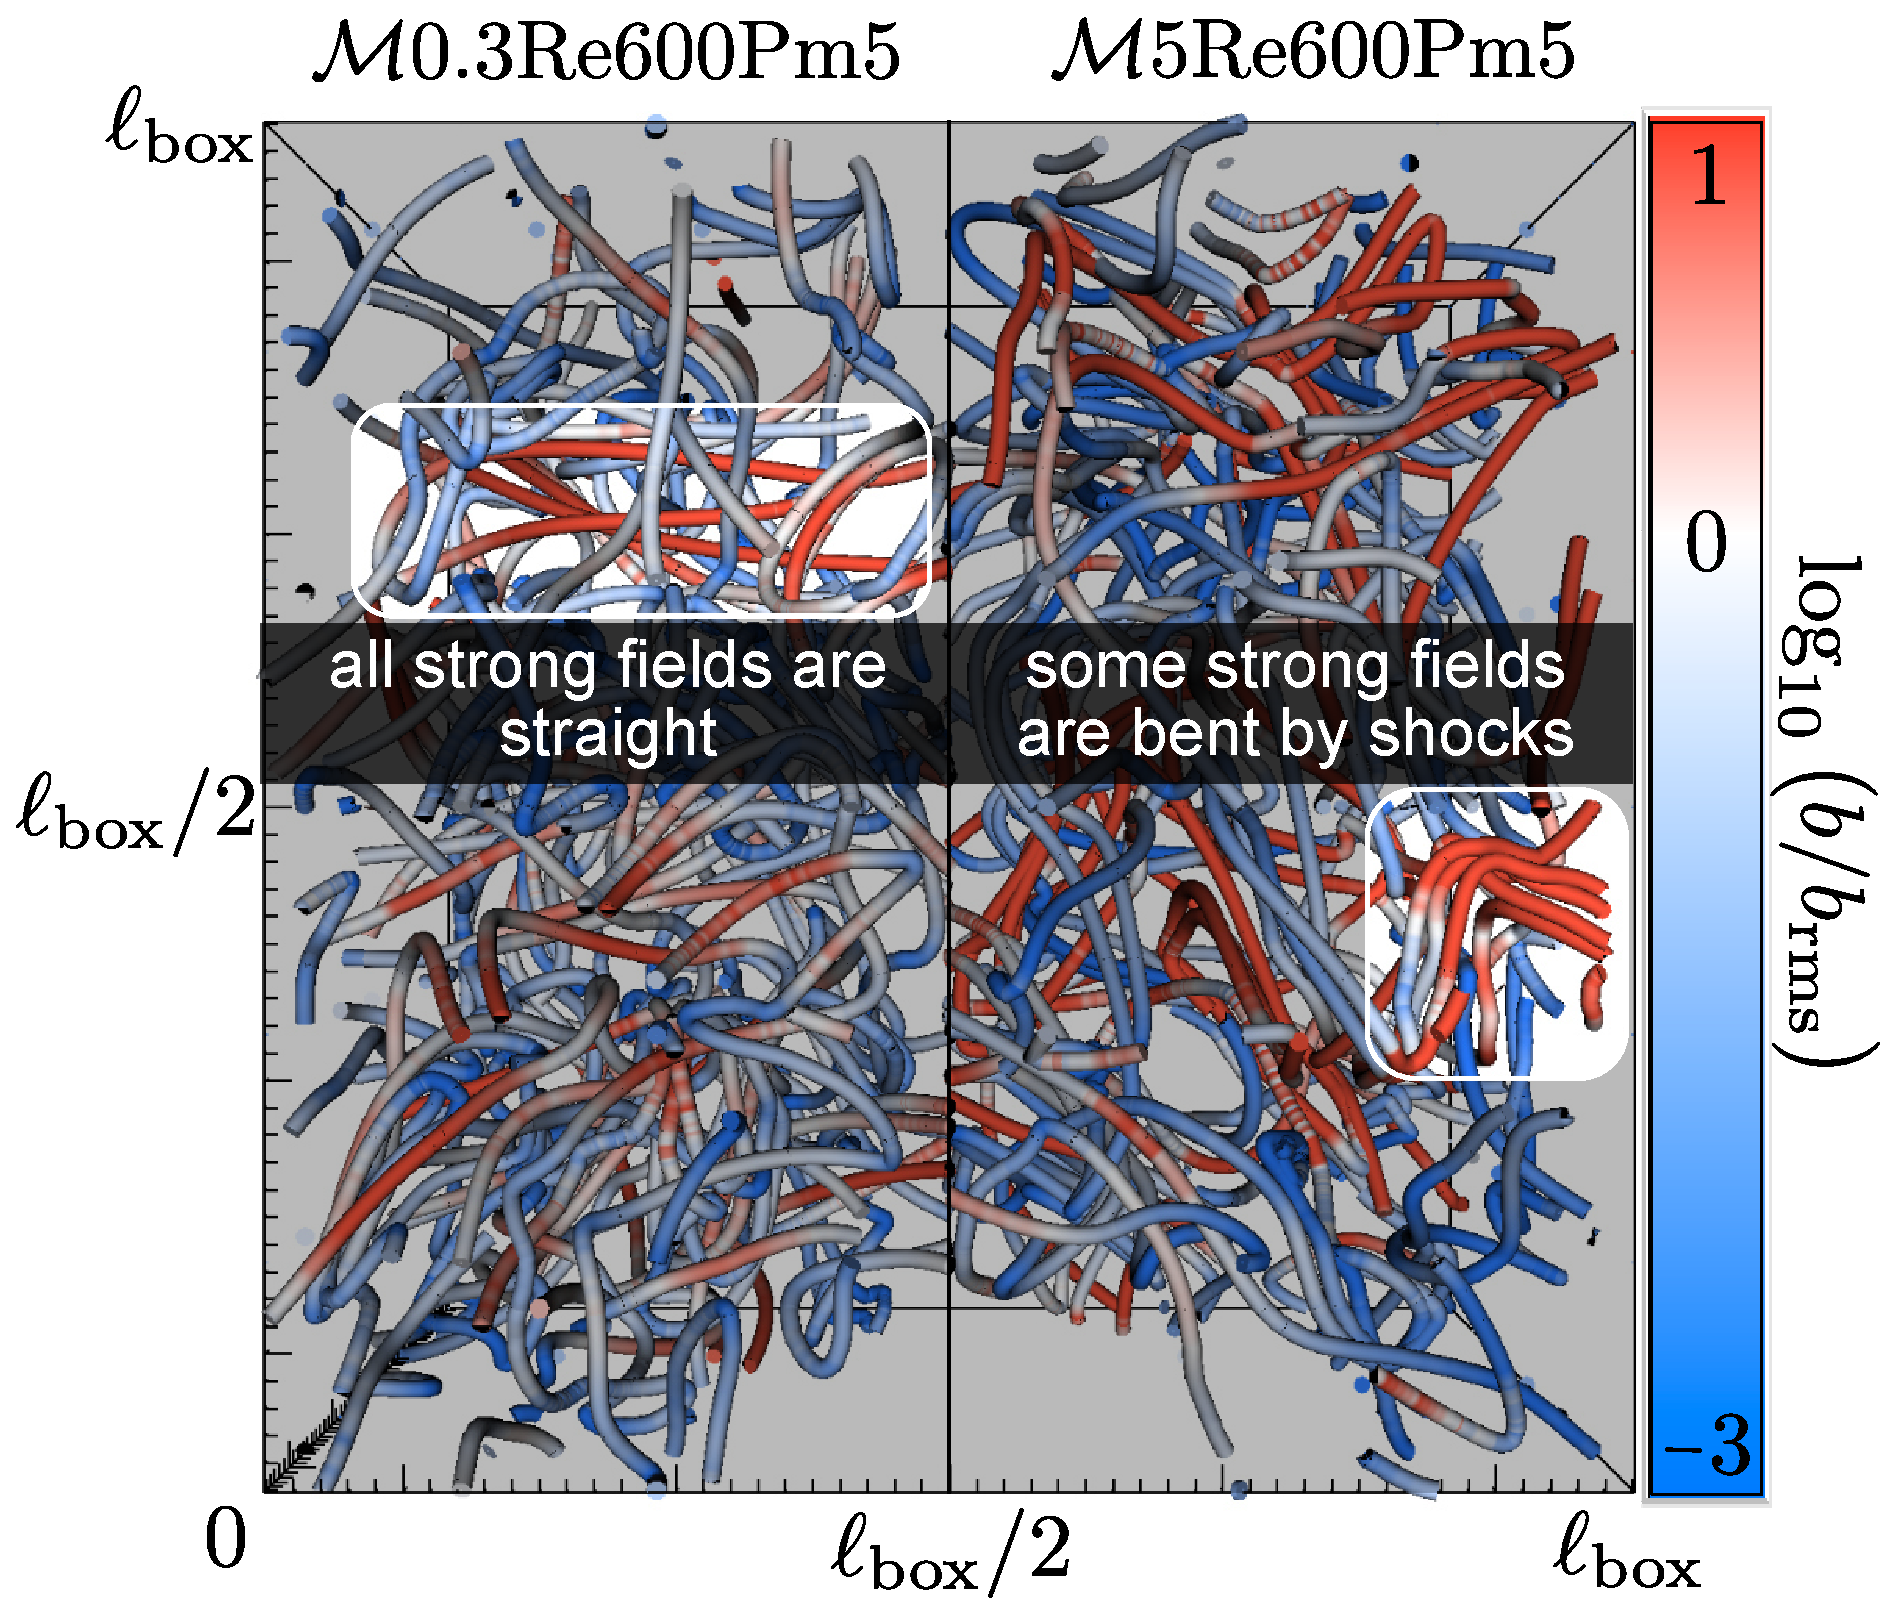
\includegraphics[width=0.65\linewidth]{figures/ssd-exp/field_lines_updated.pdf}
    \caption{Magnetic field streamlines for \SimName{0.3}{600}{5} and \SimName{5}{600}{5} plotted on the left- and right-hand side of the cube, respectively, for a time realisation midway through the kinematic phase of each simulation. Streamlines are coloured based on the normalised magnetic field magnitude, $b / b_\mathrm{rms}$, using a colour-range that spans across the same range of $b / b_\mathrm{rms}$ as plotted in the right panel of \autoref{fig:pdfs}. Notice how the relationship between field magnitude and field-line curvature (see \autoref{fig:curvature}) for \SimName{0.3}{600}{5} is readily apparent, with strong fields (red) being straight and weak fields (blue) bent, whereas for \SimName{5}{600}{5}, this relationship weakens, and some strong fields are bent significantly, and some weak fields are straight.}
    \label{fig:cube}
\end{figure}

\subsubsection{Compressible vs. Incompressible Field Geometry}

Overall, our quantitative analysis of the field geometry supports our interpretation and \citet{schekochihin2004simulations, schekochihin2002spectra}'s models for the relationship between the magnetic peak energy scale and resistive dissipation scale in the previous section: in the incompressible flow regime (where shocks are absent), the SSD in the kinematic phase produces a ``folded field'' geometry where magnetic energy becomes concentrated at $k_\eta$ -- the smallest scales possible (a state that \citet{schekochihin2004simulations} shows persists into the saturated phase), and $b \sim \kappa^{-1/2}$, but in the compressible flow regime (where shocks are ubiquitous), this correlation between the amplitude and the field geometry disappears. Again, we emphasise that the distribution of magnetic field-line curvature remains essentially the same, regardless of the flow regime, but the magnetic field amplitude distribution changes significantly, reducing the amplitude - correlation covariance and giving rise to strong deviations away from the incompressible $b \sim \kappa^{-1/2}$ relation. It would be an interesting additional avenue of exploration to understand if the correlation is re-established at small enough $\ell$, perhaps $\ell_\mathrm{s}$, the sonic scale, where the plasma transitions from supersonic to subsonic, and becomes highly-magnetised and fundamentally incompressible (see \eg \citealt{Beattie2024_10k_MHD} for an $\mReh \sim 10^6$ simulation that resolves this transition). We leave this investigation for future studies.

\section{Chapter Discussion}
\label{sec:discussion}

Our findings for the scaling behaviour of velocity and magnetic fields generated during the kinematic phase of SSDs are relevant to a wide range of astrophysical systems, but here we highlight galaxy mergers and cosmic ray propagation as two particularly interesting cases. The former case creates an environment that excites a kinematic SSD, and the latter has recently been explored in terms of underlying curvature statistics of the magnetic field. In both of these examples we highlight how it is of key importance to differentiate between the incompressible and compressible SSD regimes (see the end of \S\ref{sec:results:peak} for our distinction between these two regimes) for these astrophysical processes, since the underlying fields are completely different in these two regimes, even based on the power spectrum alone. We also motivate the importance of this distinction in regime for the transition of magnetic fields out of the kinematic phase, and into the saturated phase, which is ultimately the phase the Milky Way's ISM is in today.

\subsection{Small-Scale Dynamos in Galaxy Mergers}

Young galaxies \citep{geach2023polarized} and galaxy mergers are two environments where turbulent SSD amplified magnetic fields play a critical role in shaping the plasma dynamics \citep[\eg][]{pakmor2014magnetic, pakmor2017magnetic, martin2018three, martin2022towards, brzycki2019parameter, whittingham2021impact, whittingham2023impact, pfrommer2022simulating}. Merger events, particularly those involving gas-rich disc galaxies, are highly transformative, with strong magnetic fields influencing angular momentum transport and providing pressure support against collapse \citep{whittingham2021impact}. However, in these environments, a notable but as-yet unexplained property of the amplified magnetic fields is that magnetic energy peaks on scales of $\ell_\mathrm{p} \gtrsim \mathrm{kpc}$ during even the kinematic phase of the SSD \citep[\eg][]{rodenbeck2016magnetic, basu2017detection, brzycki2019parameter, whittingham2021impact, pfrommer2022simulating}, which is much larger than predicted by incompressible SSD theory, which limits field growth to smaller scales (\ie magnetic dissipation scale, $\ell_\eta$).

Since, \DIFdelbegin \DIFdel{here, in this study}\DIFdelend \DIFaddbegin \DIFadd{in this chapter}\DIFaddend , we have found that compressible SSDs can drive fields to larger scales than incompressible ones, it is natural to ask if considering compressibility resolves this problem. To answer this question, recall that we found that compressibility in the highly turbulent, supersonic plasma flows can shift the peak magnetic scales $\ell_\mathrm{p}$ from $\ell_\eta$ to much larger scales, even larger than the viscous scale $\ell_\nu$. The condition for this to occur is $\mPrm < \mReh^{2/3}$, where $\mReh$ and $\mPrm$ varies with plasma density, temperature, and ionisation throughout different phases of the ISM \citep{rincon2019dynamo, ferriere2019plasma, shukurov2021astrophysical, brandenburg2023galactic}. This condition is met in some phases (most notably the cold neutral medium, CNM), but not others, and it is unclear how to extend our condition to a realistic environment where different phases are intermixed and thus there is no single value of $\mReh$ and $\mPrm$. Nonetheless, even if we are generous and assume that this condition is satisfied, it is clear that compressibility alone cannot explain the large observed scales of magnetic fields in mergers, simply because the ratio $\ell_\mathrm{p}/\ell_\nu \sim \mReh^{1/3}\mPrm^{1/2}$ is not large enough -- even for the most favourable case of the CNM, for which \citet{brandenburg2023galactic} estimate $\mReh\sim 10^{10}$ and $\mPrm \sim 10^{4}$, we only have $\ell_\mathrm{p}/\ell_\nu \sim 10^5$, whereas \DIFdelbegin \DIFdel{$\ell_0/\ell_\nu \sim \mReh^{2/3} \sim 10^{7}$}\DIFdelend \DIFaddbegin \DIFadd{$\ell_\mathrm{turb}/\ell_\nu \sim \mReh^{2/3} \sim 10^{7}$}\DIFaddend . Thus, even using the most generous possible characteristic numbers, a compressible SSD would still yield a peak magnetic scale that is $\sim 2$ orders of magnitude smaller than the turbulent driving scale, which is much too small to explain the observed $\sim\mathrm{kpc}$-scale fields observed in galaxy mergers. Adopting values of $\mReh$ and $\mPrm$ for other ISM phases (especially the warm and hot phases, which are volume-filling in the disc) only strengthen this conclusion.

That said, the fact that compressibility \textit{alone} cannot explain the existence of large-scale fields in galaxy merger does not mean that it is irrelevant. While compressible SSDs still leave \DIFdelbegin \DIFdel{$\ell_0 \gg \ell_\mathrm{p}$}\DIFdelend \DIFaddbegin \DIFadd{$\ell_\mathrm{turb} \gg \ell_\mathrm{p}$}\DIFaddend , they nonetheless produce $\ell_\mathrm{p}$ that are larger than in the incompressible case by a factor of $\mReh^{1/3}$ (in \DIFdelbegin \DIFdel{highlight }\DIFdelend \DIFaddbegin \DIFadd{highly }\DIFaddend compressible, $\mSonicMach\to\infty$ plasma flows) -- a factor that, depending on the ISM phase and the large-scale velocity dispersion, ranges from hundreds to tens of thousands. The resulting intermediate-scale fields can then serve as seeds for processes such as shear from galactic rotation or gravitational and buoyancy instabilities \citep[e.g.][]{pakmor2017magnetic, steinwandel2023towards} that drive the field to yet larger scales, significantly reducing the time required for this growth compared to what would be expected if one had to begin from the smaller seed fields produce by an incompressible SSD.

\subsection{Cosmic Ray Propagation in Compressible Plasmas}

Cosmic ray propagation is a longstanding problem, the bulk of which is far beyond the scope of this \DIFdelbegin \DIFdel{paper}\DIFdelend \DIFaddbegin \DIFadd{chapter}\DIFaddend . However, there is a class of propagation models for which our conclusions regarding curvature statistics have important implications. For example, \citet{butsky2023galactic} has recently suggested that intermittent magnetic field fluctuations are necessary for regulating low-energy ($\sim \mathrm{MeV}$ -- $\mathrm{TeV}$) cosmic ray scattering in the Milky Way. \citet{kempski2023cosmic} and \citet{Lemoine2023_field_reversal_CR_transport} provide a potential source of magnetic field intermittency: intense regions of curved magnetic fields that reverse upon themselves, \ie magnetic field reversals. They argue that if magnetic fields are dominated by their fluctuating field ($\delta b/b_0 \gg 1$; as is the case for our simulations because there is no $\mVector{b}_0$) then there is an energy dependent diffusion process associated with cosmic ray particles scattering off of magnetic fields due to the field's reversal being on scales that are resonant with the gyroradius of the cosmic ray.

The \citet{kempski2023cosmic} model contains a resonance criterion derived from the assumption that $b \sim \kappa^{-1/2}$, which we have shown holds during the kinematic phase of incompressible SSDs but breaks down in compressible (\ie supersonic, turbulent) SSDs\footnote{
    It is not immediately clear whether this breakdown is relevant for cosmic ray propagation in galaxies like the Milky Way, where magnetic fields are maintained in a saturated dynamo state. While one might consider the possibility that $b \sim \kappa^{-1/2}$ breaks down for supersonic SSDs during the kinematic phase but holds in the saturated phase, this seems unlikely. In fact, \citet{schekochihin2004simulations} showed that for incompressible SSDs, the relationship between magnetic field-line curvature and field strength remains largely unchanged from the kinematic to the saturated phase, with the main difference being simply that high values of $b/b_\mathrm{rms}$ are suppressed as $b_\mathrm{rms}$ converges towards the saturated value. In a forthcoming paper we extend this result to the compressible regime, meaning that our conclusions about the implications of a breakdown in the $b\sim\kappa^{-1/2}$ relation for cosmic ray propagation apply to both high-redshift galaxies and present-day galaxies like the Milky Way.
}. Instead, \S\ref{sec:results:kappa} shows that magnetic field strength and curvature tend towards being independent in the compressible regime. That is not to say that the magnetic field does not also support reversals in the compressible regime; in probability density, it has just as many as the incompressible regime (see \autoref{fig:pdfs}). However the magnetic field amplitude is no longer constrained to a curvature relation, and hence the gyroradii of the CRs are free to vary more independently of the curvature than would be true for the incompressible case. Therefore these models will need to be modified for the $\mSonicMach > 1$ turbulent regime, where parts of the volume will have no resonances. The caveat being, we do not know how these relations scale as a function of length scale, and it could be that the required correlations emerge on small enough scales and the resonances are restored.

\subsection{The Transition out of Kinematic Growth}
\label{sec:discussion:saturation}

Finally, we would like to briefly motivate the importance of performing an analysis similar to the present study for the dynamo transition through the nonlinear and into the saturated phase. This would not only reveal the hierarchy of scales ultimately produced and sustained by SSDs in steady state, but would also determine what mechanism mediates the magnetic backreaction onto the velocity field as the magnetic energy saturates. This exercise carries direct relevance for galaxy formation, where repeated mergers induce SSD action that evolve through the kinematic phase, which we have studied here, and converge on a remnant ISM where the post-merger galaxy is maintained in the saturated phase of the SSD. It is therefore important for building an understanding of the magnetic fields that provide the backdrop for all post-merger interstellar processes.

For an incompressible SSD, \citet{schekochihin2001structure, schekochihin2002small, schekochihin2004simulations} first predicted, and \citetalias{kriel2022fundamental} confirmed with DNSs, that during the kinematic phase where $E_\mathrm{mag}(\ell) \ll E_\mathrm{kin}(\ell)$ for all $\ell$, magnetic fields naturally become organised into a folded field geometry with magnetic energy concentrated at the smallest scales allowed by magnetic dissipation \citep[see also \eg][]{brandenburg2023dissipative}, namely $\ell_\mathrm{p} \sim \ell_\eta$. In this phase magnetic fields are most rapidly grown through stretching motions \DIFdelbegin \DIFdel{\mbox{%DIFAUXCMD
\citep{beattie2023bulk} }\hskip0pt%DIFAUXCMD
}\DIFdelend \DIFaddbegin \DIFadd{\mbox{%DIFAUXCMD
\citep{cho2009growth, beattie2023bulk} }\hskip0pt%DIFAUXCMD
}\DIFaddend induced by viscous fluctuations, since these fluctuations have the shortest turnover time (see \S\ref{sec:results:dissipation:keta}). These fluctuations, however, cannot remain the most efficient driver of SSD growth indefinitely. Once the magnetic field reaches an amplitude where $\mVector{u}\cdot\nabla\mVector{u} \sim \mVector{b}\cdot\nabla\mVector{b}$, it suppresses hydrodynamic motions on that scale. Following \citet{schekochihin2002model}, this happens when $E_\mathrm{mag} \sim E_\mathrm{kin}(\ell_\mathrm{s})$, where in the kinematic phase, the stretching scale is $\ell_\mathrm{s} \sim \ell_\nu$. Once stretching on $\ell_\nu$ becomes suppressed, SSD action is expected to transition into a reduced growth regime. For incompressible SSDs, there is a theoretical consensus that magnetic energy growth transitions to linear-in-time \citep{cho2009growth, beresnyak2012universal, Xu2016_dynamo, seta2020saturation}, characterised by $E_\mathrm{mag} \sim \varepsilon t$ (see \autoref{fig:time_evolution}).

The situation is less clear for compressible SSDs, where there is an ongoing debate about whether the growth mechanism is universal, or if SSDs in the presence of \citet{burgers1948_turbulence_model}-like turbulence transition into quadratic-in-time regime, $E_\mathrm{mag} \sim t^2$, as proposed by \citet{Schleicher2013_quadratic_growth}. Regardless of the answer to this question, the mechanism behind the backreaction is thought to be generally similar to the incompressible case: $\ell_\mathrm{s}$ shifts from $\ell_\nu$ to the next smallest unsuppressed turbulent fluctuations. Since these fluctuations are larger than the viscous-scale fluctuations, they have longer turnover times, and thus generate magnetic flux at a slower rate \DIFdelbegin \DIFdel{\mbox{%DIFAUXCMD
\citep{Schober2015_dynamo_saturation}}\hskip0pt%DIFAUXCMD
}\DIFdelend \DIFaddbegin \DIFadd{\mbox{%DIFAUXCMD
\citep{Schober2015_dynamo_saturation, galishnikova2022tearing}}\hskip0pt%DIFAUXCMD
}\DIFaddend . Magnetic amplification continues to suppress progressively larger scales \textit{ad infinitum}, until the dynamo saturates at the driving scale, with $\ell_\mathrm{p} > \ell_\nu$. This has very clearly been shown in the time-dependent spectral ratios in \citet{beattie2022growth} and \citet{beattie2023bulk}. Various phenomenological models that describe the details of this process have been proposed, but they have never been tested at a fundamental level using DNSs, and it is unclear exactly which details of the incompressible picture are extensible to the compressible regime. Thus, in the \DIFdelbegin \DIFdel{third part of this series}\DIFdelend \DIFaddbegin \DIFadd{next chapter}\DIFaddend , we will explore the statistics of the nonlinear and saturated phase using the comprehensive dataset we have built in this \DIFdelbegin \DIFdel{study}\DIFdelend \DIFaddbegin \DIFadd{chapter}\DIFaddend , as well as in \citetalias{kriel2022fundamental}. Where it is important to reveal the mechanism, and thereby the timescale, of the backreaction, as this process also provides an avenue for generating ``large-scale'' magnetic fields, in addition to LSDs (see the Introduction and the previous section for a discussion), and thus play an important role in the context of explaining $\sim \mathrm{kpc}$ fields observed in young and merger-disturbed galaxies.

\section{Chapter Summary \& Conclusions}
\label{sec:conclusion}

In this \DIFdelbegin \DIFdel{study }\DIFdelend \DIFaddbegin \DIFadd{chapter }\DIFaddend we explore how both the energy spectrum (see \S\ref{sec:results:peak}) and field-line curvature (see \S\ref{sec:results:kappa}) of magnetic fields produced during the exponential-growing (kinematic) phase of small-scale dynamos (SSDs) depend upon the plasma flow regime (from subsonic $\mSonicMach < 1$ to supersonic $\mSonicMach > 1$, and viscous $\mReh < \mReh_\mathrm{crit} \approx 100$ to turbulent $\mReh \geq \mReh_\mathrm{crit}$ flows). To do so, we have used DNSs where we explicitly control the velocity field magnitude, as well as the dissipation rates of kinetic and magnetic energy to explore a wide range of $\mSonicMach$, hydrodynamic Reynolds number, $\mReh$, and magnetic Prandtl number, $\mPrm$. This has allowed us to extend our understanding of $\mPrm \geq 1$ SSD-amplified magnetic fields into the previously poorly-understood regime of supersonic SSDs. In particular, we have identified new relationships between the important characteristic length scales in a SSD -- the outer scale of turbulence \DIFdelbegin \DIFdel{$\ell_0$}\DIFdelend \DIFaddbegin \DIFadd{$\ell_\mathrm{turb}$}\DIFaddend , the kinetic energy dissipation scale $\ell_\nu$, the magnetic energy dissipation scale $\ell_\eta$, and the peak magnetic energy scale $\ell_\mathrm{p}$ -- as a function of the fundamental plasma numbers: $\mSonicMach$, $\mReh$, and $\mPrm$. We complement this with a study of the statistics of magnetic field-line curvature, which support our findings.

We list our key results below:
\begin{itemize}
    \item During the kinematic phase of SSDs, the kinetic energy dissipation scale $\ell_\nu$ varies with $\mReh$ and $\mSonicMach$ as expected for hydrodynamic flows (see the left panel in \autoref{fig:dissipation_scaling}). That is, we find three regimes: \DIFdelbegin \DIFdel{$\ell_\nu \sim \ell_0 \,\mReh^{-3/4}$ }\DIFdelend \DIFaddbegin \DIFadd{$\ell_\nu \sim \ell_\mathrm{turb} \,\mReh^{-3/4}$ }\DIFaddend for subsonic, turbulent flows (where $\mSonicMach \leq 1$ and $\mReh \geq \mReh_\mathrm{crit}$), which corresponds with \citet{kolmogorov1941dissipation}-like scaling, \DIFdelbegin \DIFdel{$\ell_\nu \sim \ell_0 \,\mReh^{-2/3}$ }\DIFdelend \DIFaddbegin \DIFadd{$\ell_\nu \sim \ell_\mathrm{turb} \,\mReh^{-2/3}$ }\DIFaddend for supersonic ($\mSonicMach > 1$) flows, which corresponds with \citet{burgers1948_turbulence_model}-like scaling, and finally \DIFdelbegin \DIFdel{$\ell_\nu \sim \ell_0 \,\mReh^{-3/8}$ }\DIFdelend \DIFaddbegin \DIFadd{$\ell_\nu \sim \ell_\mathrm{turb} \,\mReh^{-3/8}$ }\DIFaddend for viscous, subsonic flows (where $\mSonicMach \leq 1$ and $\mReh < \mReh_\mathrm{crit}$ first shown in \citetalias{kriel2022fundamental}). \\

    \item The magnetic dissipation scale $\ell_\eta$ is related to the kinetic dissipation scale as $\ell_\eta \sim \ell_\nu \,\mPrm^{-1/2}$ in all $\mPrm \geq 1$ turbulent plasma flow regimes. Since this scaling relation, first proposed by \citet{schekochihin2002spectra}, follows from assuming that $\ell_\eta$ is located on the scale where the viscous shearing rate is balanced by Ohmic dissipation, we conclude that the viscous (smallest-scale) kinetic fluctuations are always the most efficient at amplifying magnetic energy during the kinematic phase of $\mPrm \geq 1$ SSDs, invariant to the $\mSonicMach$ of the plasma. \\

    \item The magnetic peak scale $\ell_\mathrm{p}$ and the associated statistics of the magnetic field-line curvature $\kappa$ produced by SSDs are very different for \textit{incompressible} (\ie either $\mSonicMach \leq 1$, or $\mSonicMach > 1$ and $\mReh < \mReh_\mathrm{crit}$) and \textit{compressible} (\ie $\mSonicMach > 1$ and $\mReh \geq \mReh_\mathrm{crit}$) flows. The incompressible case behaves as predicted by the ``folded field'' model of \citet{schekochihin2002spectra, schekochihin2004simulations}, where the field-line curvature $\kappa$ and the field magnitude $b$ are strongly anti-correlated (see \autoref{fig:curvature}) as $b \sim \kappa^{-1/2}$, and the magnetic energy becomes concentrated on the smallest scales allowed by magnetic dissipation, which results in the hierarchy of characteristic length scales \DIFdelbegin \DIFdel{$\ell_0 > \ell_\nu > \ell_\eta \sim \ell_\mathrm{p}$}\DIFdelend \DIFaddbegin \DIFadd{$\ell_\mathrm{turb} > \ell_\nu > \ell_\eta \sim \ell_\mathrm{p}$}\DIFaddend . By contrast, in the compressible regime, supersonic turbulence naturally gives rise to shocks with characteristic shock width $\ell_\mathrm{shock} \sim \mSonicMach^2 / (\mReh\, (\mSonicMach-1)^2)$, which we derive in \S\ref{sec:results:peak}. These shocks create magnetic structures via flux-freezing and compression, which change the distribution of $b$ amplitudes, essentially destroying the anti-correlation between $b$ and $\kappa$, but notably, does not change the distribution of field-line curvature. These (isotropic) shocks also concentrate magnetic fields on a scale \DIFdelbegin \DIFdel{$\ell_\mathrm{p} \sim (\ell_0/\ell_\mathrm{shock})^{1/3} \ell_\eta \gg \ell_\eta$}\DIFdelend \DIFaddbegin \DIFadd{$\ell_\mathrm{p} \sim (\ell_\mathrm{turb}/\ell_\mathrm{shock})^{1/3} \ell_\eta \gg \ell_\eta$}\DIFaddend , where, in the $\mSonicMach\to\infty$ limit, this produces $\ell_\mathrm{p} \sim \mReh^{1/3} \ell_\eta$. In plasmas where $\mPrm < \mReh^{2/3}$, the subviscous range is smaller than the net shift in $\ell_\mathrm{p}$ to larger scales (from $\ell_\eta$), which gives rise to a hierarchy \DIFdelbegin \DIFdel{$\ell_0 > \ell_\mathrm{p} > \ell_\mathrm{shock} > \ell_\nu > \ell_\eta$}\DIFdelend \DIFaddbegin \DIFadd{$\ell_\mathrm{turb} > \ell_\mathrm{p} > \ell_\mathrm{shock} > \ell_\nu > \ell_\eta$}\DIFaddend . Moreover, in the compressible regime, magnetic field-line curvature and magnitude tend towards independence, $b \sim \kappa^0$. \\

    \item We discuss a longstanding problem about the generation of large-scale magnetic fields in the context of galaxy mergers (but potentially can be more broadly applied to other young galaxies, such as the recent observation of a young starburst galaxy with a large-scale field in \citealt{geach2023polarized}). Since the turbulence in these galaxies is likely supersonic due to high gas densities that favour rapid cooling, the SSDs within them are likely compressible rather than incompressible. We show that this is not by itself sufficient to explain the large-scale fields observed in these galaxies, because, while compressibility increases the characteristic field size by many orders of magnitude compared to the incompressible case (at least for some combinations of plasma parameters), this increase still leaves fields concentrated on scales much smaller than those observed. Nonetheless, we argue that the increase in field size scale enabled by compressibility have the potential to help accelerate other, larger-scale dynamo mechanisms that produce large-scale fields. \\

    \item We discuss the implications our results have on models of cosmic ray scattering based on resonances between the size-scale of magnetic field reversals and the gyro-radius of the cosmic ray, \citep[e.g.,][]{kempski2023cosmic}. We suggest that for supersonic plasmas, which may be a significant portion of the interstellar medium of the Milky Way, these resonances may not work, since the magnetic field amplitude ($\sim$ gyro-radius) and underlying field curvature become independent from one another, at least in the sense that the global correlation reduces between the curvature and field amplitude.
\end{itemize}

\section*{Chapter Acknowledgements}
We thank the reviewer for their feedback, as well as Amitava Bhattacharjee, Axel Brandenburg, Frederick Gent, Pierre Lesaffre, Philipp Kempski, Mordecai-Mark Mac Low, Sergio Martin Alvarez, Christoph Pfrommer, Bart Ripperda, Alexander Schekochihin, Anvar Shukurov, Juan Diego Soler, and Enrique V\'azquez-Semadeni, along with Naomi M. McClure-Griffiths' research group, especially Yik Ki (Jackie) Ma, Hilay Shah, and Lindsey Oberhelman, for helpful discussions which have greatly improved the quality of this \DIFdelbegin \DIFdel{study}\DIFdelend \DIFaddbegin \DIFadd{chapter}\DIFaddend .

N.~K. acknowledges financial support from the Australian Government via the Australian Government Research Training Program Fee-Offset Scholarship and the Research School of Astronomy \& Astrophysics for the Joan Duffield Research Award. J.~R.~B.~acknowledges financial support from the Australian National University, via the Deakin PhD and Dean's Higher Degree Research (theoretical physics) Scholarships, the Australian Government via the Australian Government Research Training Program Fee-Offset Scholarship, and the Australian Capital Territory Government funded Fulbright scholarship. C.~F.~acknowledges funding provided by the Australian Research Council (Future Fellowship FT180100495 and Discovery Project DP230102280), and the Australia-Germany Joint Research Cooperation Scheme (UA-DAAD). C.~F.~further acknowledges high-performance computing resources provided by the Leibniz Rechenzentrum and the Gauss Centre for Supercomputing (grants~pr32lo, pr48pi and GCS Large-scale project~10391), the Australian National Computational Infrastructure (grant~ek9) and the Pawsey Supercomputing Centre (project~pawsey0810) in the framework of the National Computational Merit Allocation Scheme and the ANU Merit Allocation Scheme. M.~R.~K acknowledges support from the Australian Research Council through its Discovery Projects and Laureate Fellowships funding schemes, awards DP230101055 and FL220100020 and from the Australian National Computational Merit Allocation Scheme awards at the National Computational Infrastructure and the Pawsey Supercomputing Centre (award jh2). J.~K.~J.~H. acknowledges funding via the ANU Chancellor’s International Scholarship, the Space Plasma, Astronomy \& Astrophysics Higher Degree Research Award, and the Boswell Technologies Endowment Fund.

The authors acknowledge valuable discussions that took place during the Nordita workshop, ``Towards a Comprehensive Model of the Galactic Magnetic Field,'' which was supported by NordForsk and the Royal Astronomical Society, as well as the Interstellar Institute's program ``II6,'' hosted at the Institut Pascal at Paris-Saclay University, which nourished the development of the ideas in this work.

The simulation software, \textsc{flash}, was in part developed by the Flash Centre for Computational Science at the Department of Physics and Astronomy of the University of Rochester. As discussed in \S\ref{sec:ICs:Mach}, we produce a turbulent forcing field, $\mVector{f}$, via \textsc{TurbGen} developed by \citet{federrath2010comparing}. We also relied on the following programming languages/packages to analyse our simulation data and produce visualisations: \textsc{C++} \citep{stroustrup2013cpp}, \textsc{python} along with \textsc{numpy} \citep{oliphant2006guide, van2011numpy, harris2020array}, \textsc{matplotlib} \citep{hunter2007matplotlib, bisong2019matplotlib}, and \textsc{cython} \citep{behnel2010cython, smith2015cython}, as well as the \textsc{WebPlotDigitizer} app \citep{Rohatgi2022} and \textsc{visit} \citep{childs2012visit}.

\section{Chapter End Matter}

\subsection{Density-Weighted Hydrodynamic Reynolds Number}
\label{app:knu:density_weighted}

\begin{figure}
    \centering
    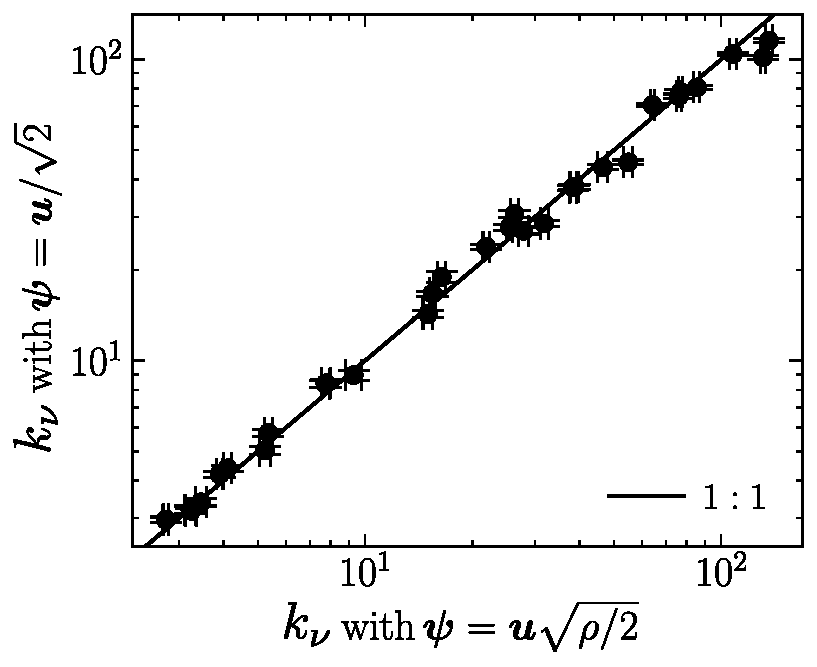
\includegraphics[width=0.65\linewidth]{figures/ssd-exp/scaling_knu_comparison.pdf}
    \caption{For each simulation setup in \autoref{table:ssd-exp:summary}, we compare the converged (see \S\ref{sec:results:nres} for details) characteristic viscous wavenumber, $k_\nu$, measured from \autoref{eqn:knu_measure} constructed with $\mVector{\psi} = \mVector{u} / \sqrt{2}$ (y-axis; studied in the main text), and $k_\nu$ constructed with $\mVector{\psi} = \mVector{u} \sqrt{\rho/2}$ (x-axis). We find that our measurement of $k_\nu$ is insensitive to the inclusion of density ($\rho$) variations in the plasma.}
    \label{fig:hydro_reynolds_compared}
\end{figure}

In the main text (see \S\ref{sec:tools:k_nu}) we measured characteristic viscous wavenumbers, $k_\nu$, from kinetic energy spectra, $E_\mathrm{kin}(k)$, constructed only from the velocity field (that is, $\mVector{\psi} = \mVector{u}/\sqrt{2}$ in \autoref{eqn:kin_fourier}). An alternative, popular definition for compressible flows \citep[see for example][]{federrath2010comparing, federrath2013universality, schmidt2019kinetic, grete2021matter, grete2023matter}, which accounts for density fluctuations, is $E_\mathrm{kin}(k)$ constructed from \autoref{eqn:kin_fourier} with $\mVector{\psi} = \mVector{u} \sqrt{\rho/2}$. This definition is based on the idea that $E_\mathrm{kin}$ should have units of kinetic energy, and such that $\psi^2$ needs to be a positive definite quantity \citep{kida1990energy}.

In \autoref{fig:hydro_reynolds_compared} we compare converged (with numerical resolution; see \S\ref{sec:results:nres}) $k_\nu$ measured from both definitions for $E_\mathrm{kin}(k)$, for all our simulations, plotting $k_\nu$ derived from the $\mVector{\psi} = \mVector{u} \sqrt{\rho/2}$ spectrum on the x-axis, and $\mVector{\psi} = \mVector{u} / \sqrt{2}$ on the y-axis. We show that $k_\nu$ measured from the different definitions for $E_\mathrm{kin}(k)$ scales 1:1, and therefore our measurements for $k_\nu$ in the kinematic phase of the SSD are robust and insensitive to density fluctuations, even for our $\mSonicMach > 1$ simulations.

\subsection{Resistive Scale Measured from the Magnetic Reynolds Spectrum}
\label{app:krm}

\begin{figure}
    \centering
    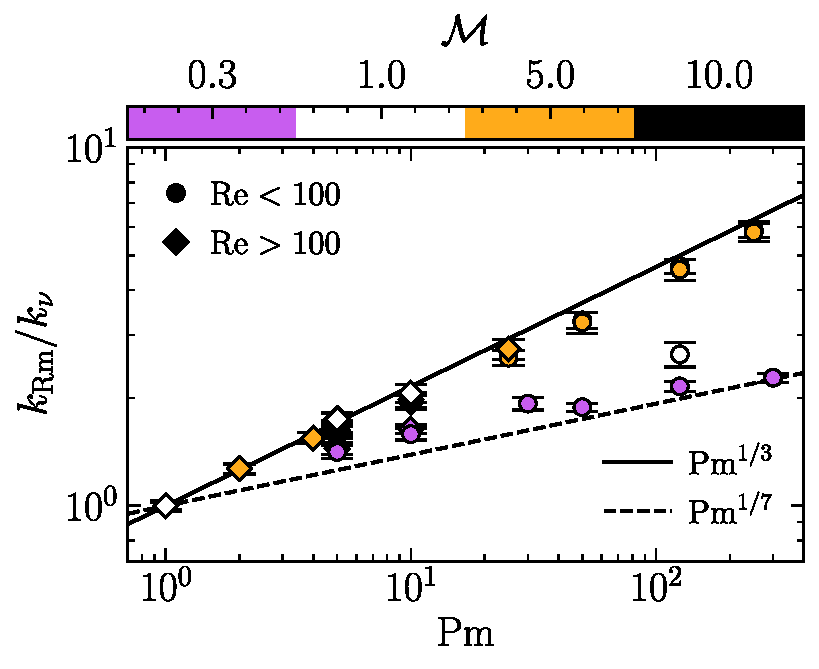
\includegraphics[width=0.65\linewidth]{figures/ssd-exp/scaling_keta_mag.pdf}
    \caption{For each simulation in \autoref{table:ssd-exp:summary}, we plot the separation between the wavenumber where the magnetic Reynolds number is one ($k_\mathrm{Rm} : \mRem(k) = 1$), and the viscous wavenumber ($k_\nu$; using the definition in the main text, see \S\ref{sec:tools:k_nu}), via $k_\mathrm{Rm}/k_\nu$, and compare this scale separation with the magnetic Prandtl number. We plot simulations with $\mReh < \mReh_\mathrm{crit} \approx 100$ as circles, and $\mReh \geq \mReh_\mathrm{crit}$ as diamonds, and colour points by the sonic Mach number. We also annotate two power laws $\mPrm^{1/3}$ (solid line) and $\mPrm^{1/7}$ (dashed line) to highlight the different empirical scaling of $k_\mathrm{Rm}/k_\nu$ for subsonic and supersonic SSDs. Since $k_\mathrm{Rm}$ does not return a scaling consistent with $\mPrm^{1/2}$, as we previously found in \citetalias{kriel2022fundamental} for $\mSonicMach < 1$ flows, we conclude that this measurement does not effectively probe magnetic dissipation, unlike $k_\nu : \mReh(k) = 1$, which accurately probes the dissipation of the kinetic flow.}
    \label{fig:Rm_scaling}
\end{figure}

Given the success of our definition for the viscous scale (\autoref{eqn:knu_measure}), one may be tempted to define the resistive scale analogously. That is
\begin{align}
    k_\mathrm{Rm}(t)
        = \texttt{argmin}_k\Big[
            \mathcal{I}\Big\{ \Big| \mRem(k, t) - 1 \Big| \Big\}
        \Big]
        , \label{eqn:Rm_measure}
\end{align}
where \DIFdelbegin \DIFdel{$\mRem(k, t) \equiv u_0(k, t) / \eta k$}\DIFdelend \DIFaddbegin \DIFadd{$\mRem(k, t) \equiv u_\mathrm{turb}(k, t) / \eta k$}\DIFaddend . However, in \autoref{fig:Rm_scaling} we show that this wavenumber, $k_\mathrm{Rm}$, does not correspond with $k_\eta$ derived from \autoref{eqn:keta_measure}. In this figure we plot the separation between the converged (with numerical resolution; see \S\ref{sec:results:nres}), time averaged (over the kinematic phase) $k_\mathrm{Rm}$ and $k_\nu$, for each of our simulations in \autoref{table:ssd-exp:summary}, and show that this separation does not scale like $\mPrm^{1/2}$, which we showed in \autoref{fig:dissipation_scaling} is the case irrespective of the flow regime.

We interpret this to mean that, whilst a unit analysis of the magnetic Reynolds number gives \DIFdelbegin \DIFdel{$\mRem \sim u_0 \ell_0 / \eta$}\DIFdelend \DIFaddbegin \DIFadd{$\mRem \sim u_\mathrm{turb} \ell_\mathrm{turb} / \eta$}\DIFaddend , more directly, $\mRem$ (\autoref{dfn:Reym}) controls the relative importance of the induction term, $\nabla\times(\mVector{u}\times\mVector{b})$, compared with magnetic dissipation, $\eta\nabla\times\mVector{j}$. However, each of these terms operate on different characteristic scales, (scales associated with $\ell_\nu$ for the induction, as we showed in \autoref{fig:dissipation_scaling}, and scales associated with $\ell_\eta$ for the dissipation). These details are not captured by only considering the influence of \DIFdelbegin \DIFdel{$u_0 \ell_0 / \eta$}\DIFdelend \DIFaddbegin \DIFadd{$u_\mathrm{turb} \ell_\mathrm{turb} / \eta$}\DIFaddend , \ie only considering the velocity structures for building the scale dependence (as we did with \autoref{eqn:reynolds_spectrum}). In fact, we know from \S\ref{sec:results:dissipation} that $k_\eta$ should be largely independent of the kinetic cascade statistics, which \autoref{eqn:Rm_measure} is completely dependent upon (along with the material properties of the magnetic field).

\subsection{Magnetic correlation scale}
\label{app:kcor}

\begin{figure}
    \centering
    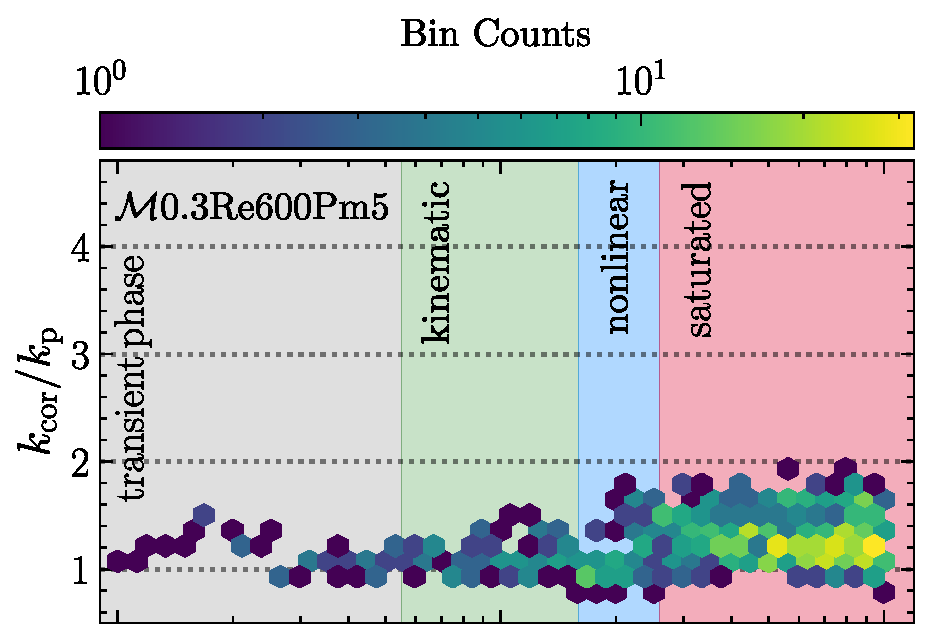
\includegraphics[width=0.65\linewidth]{figures/ssd-exp/kcor_Mach0.3_updated.pdf}
    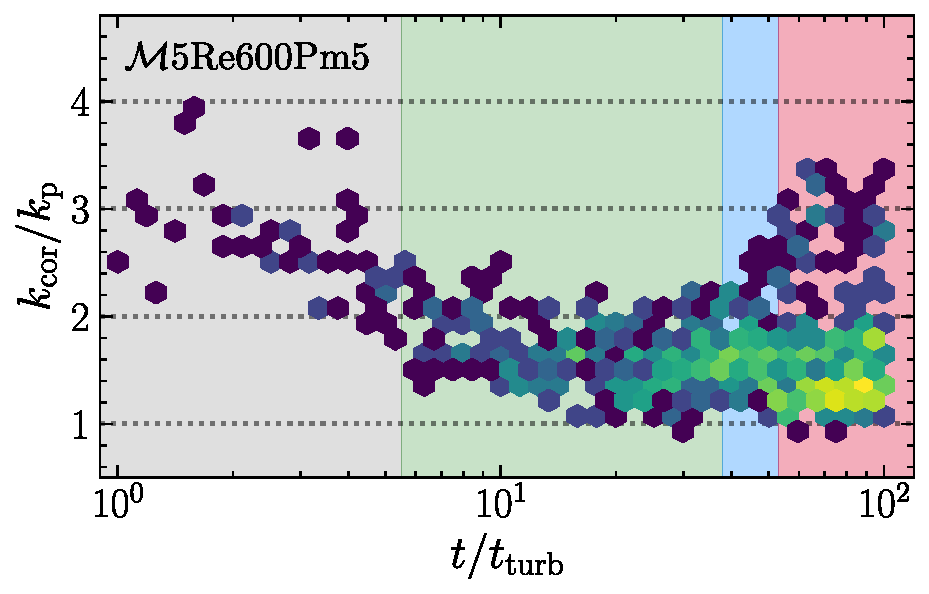
\includegraphics[width=0.65\linewidth]{figures/ssd-exp/kcor_Mach5.pdf}
    \caption{Time evolution of the magnetic correlation scale ($k_\mathrm{cor}$; from \autoref{eqn:cor_scale}), compared with the magnetic peak scale ($k_\mathrm{p}$; from \autoref{eqn:kp_measure}), for \SimName{0.3}{600}{5} and \SimName{5}{600}{5} in the top and bottom panels, respectively. We highlight the transient phase of the simulation in grey, followed by the kinematic, nonlinear, and saturated SSD phases in green, blue, and red, respectively.}
    \label{fig:mag_scales}
\end{figure}

\citet{schekochihin2004simulations} and \citet{galishnikova2022tearing} assume that the magnetic correlation (coherence) wavenumber,
\begin{align}
    k_\mathrm{cor}(t)
        &= \frac{
                \int_{0}^{\infty} E_\mathrm{mag}(k, t) \,\mdd{k}
            }{
                \int_{0}^{\infty} k^{-1} E_\mathrm{mag}(k, t) \,\mdd{k}
            }
        , \label{eqn:cor_scale}
\end{align}
is proportional to the magnetic peak wavenumber, $k_\mathrm{p}$, which \citet{beattie2022growth} showed seemed to be qualitatively true not only in the kinematic phase, but also in the saturated phase. It is not clear whether this assumption would be valid for supersonic SSD amplified fields, where the magnetic energy spectrum is broadened by shocks when $\mSonicMach > 1$ (see the bottom panel in \autoref{fig:cur_mag_spectra}). To test this, we compute $k_\mathrm{cor}$ and $k_\mathrm{p}$ for our two representative simulations, \SimName{0.3}{600}{5} and \SimName{5}{600}{5} at $N_\mathrm{res} = 576$. In \autoref{fig:mag_scales} we compare the time evolution of these two scales by plotting $k_\mathrm{cor}/k_\mathrm{p}$ computed throughout the simulation for both setups. We colour individual hexagon-bins based on the number of occurrences, and shade the time range corresponding with the transient, kinematic, nonlinear, and saturated phases grey, green, blue, and red, respectively.

As expected for \SimName{0.3}{600}{5}, we find evidence that during the kinematic phase $k_\mathrm{cor} \sim k_\mathrm{p}$, however, this relationship appears to weaken in the saturated state. For \SimName{5}{600}{5} we find that $k_\mathrm{cor} > k_\mathrm{p}$ at all times, where initially $k_\mathrm{cor} \gg k_\mathrm{p}$ due to shocks compressing magnetic energy into long, thin (\ie filamentary) structures, which broaden the magnetic energy distribution. The typical length of these shocked regions contributes energy to low-$k$ modes, while their typical width (see our model \autoref{eqn:shock_width}) contributes energy to high-$k$ modes. As the magnetic energy gradually amplifies and approaches saturation, the magnetic field becomes strong enough to suppress deformation on the smallest scales. Consequently, the ratio $k_\mathrm{cor} / k_\mathrm{p}$ tends toward $\gtrsim 1$.

\subsection{Fit Parameters Derived from Measuring Scale Convergence}

In \S\ref{sec:results:nres} we highlighted numerical convergence for two of our representative simulations, namely \SimName{0.3}{600}{5} and \SimName{5}{600}{5}. We also performed the same convergence study for all of our other simulation setups in \autoref{table:ssd-exp:summary}, so here, for each of our simulation setups, we list the two fitted parameters: (1) critical numerical resolution, $N_{\mathrm{res}, \mathrm{crit}}$, required for wavenumber convergence, and (2) the rate of convergence, $R$, for the viscous (column 2), resistive (column 3), and magnetic peak wavenumbers (column 4).

For all of our viscous simulations, where $\mReh < \mReh_\mathrm{crit} \approx 100$, we find that our measurement for $k_\nu$ (and $k_\mathrm{p}$ in the case of \SimName{5}{10}{25}) converged at even our lowest resolution runs (\ie as expected, we do not need much resolution to resolve low-$\mReh$ dynamics). In these cases, we report the lowest resolution run we performed as $N_{\mathrm{res}, \mathrm{crit}}$, and report no value for $R$, in \autoref{table:ssd-exp:nres}.

\begin{table}
\caption{Convergence properties of characteristic MHD wavenumbers.}
\label{table:ssd-exp:nres}

\renewcommand{\arraystretch}{1.05}
\setlength{\tabcolsep}{5pt}

\centeronpage{%
\scalebox{0.85}{%
\begin{threeparttable}
\begin{tabular}{l cc l cc l cc}
\hline
\hline
    \multicolumn{1}{c}{Sim. ID}
        & \multicolumn{2}{c}{$k_\nu$}
        && \multicolumn{2}{c}{$k_\eta$}
        && \multicolumn{2}{c}{$k_\mathrm{p}$} \\
    \cline{2-3} \cline{5-6} \cline{8-9} \\[-1.5ex]
        &  $N_\mathrm{res, crit}$ & $R$
        && $N_\mathrm{res, crit}$ & $R$
        && $N_\mathrm{res, crit}$ & $R$ \\
    \multicolumn{1}{c}{(1)}
        & \multicolumn{2}{c}{(2)}
        && \multicolumn{2}{c}{(3)}
        && \multicolumn{2}{c}{(4)} \\
\hline
\hline
\multicolumn{9}{c}{$\mSonicMach = 0.3$} \\
\hline
$\mSonicMach$0.3Re500Pm1
	& $34.7 \pm 1.9$ & $0.8 \pm 0.1$
	&& $67.8 \pm 8.7$ & $1.0 \pm 0.2$
	&& $31.6 \pm 13.4$ & $0.9 \pm 0.8$ \\
$\mSonicMach$0.3Re100Pm5
	& $18.0$ & --
	&& $54.4 \pm 10.4$ & $1.0 \pm 0.2$
	&& $31.4 \pm 14.7$ & $0.9 \pm 1.0$ \\
$\mSonicMach$0.3Re50Pm10
	& $18.0$ & --
	&& $49.9 \pm 7.5$ & $1.1 \pm 0.3$
	&& $32.5 \pm 12.0$ & $1.2 \pm 1.0$ \\
$\mSonicMach$0.3Re10Pm50
	& $18.0$ & --
	&& $54.5 \pm 12.6$ & $0.8 \pm 0.2$
	&& $25.8 \pm 15.3$ & $0.8 \pm 0.8$ \\
$\mSonicMach$0.3Re3000Pm1
	& $116.8 \pm 5.0$ & $1.0 \pm 0.1$
	&& $229.2 \pm 19.0$ & $1.1 \pm 0.1$
	&& $169.7 \pm 32.4$ & $1.0 \pm 0.1$ \\
$\mSonicMach$0.3Re600Pm5
	& $43.0 \pm 2.2$ & $0.8 \pm 0.1$
	&& $190.4 \pm 20.2$ & $1.0 \pm 0.1$
	&& $117.2 \pm 40.1$ & $0.8 \pm 0.2$ \\
$\mSonicMach$0.3Re300Pm10
	& $23.9 \pm 0.9$ & $0.9 \pm 0.1$
	&& $120.3 \pm 15.0$ & $1.1 \pm 0.1$
	&& $84.8 \pm 26.6$ & $1.0 \pm 0.3$ \\
$\mSonicMach$0.3Re100Pm30
	& $18.0$ & --
	&& $124.3 \pm 21.0$ & $1.0 \pm 0.1$
	&& $89.2 \pm 35.2$ & $0.9 \pm 0.3$ \\
$\mSonicMach$0.3Re24Pm125
	& $18.0$ & --
	&& $102.4 \pm 12.9$ & $1.0 \pm 0.1$
	&& $77.3 \pm 37.5$ & $0.8 \pm 0.3$ \\
$\mSonicMach$0.3Re10Pm300
	& $18.0$ & --
	&& $102.4 \pm 21.6$ & $0.9 \pm 0.1$
	&& $82.2 \pm 27.1$ & $0.9 \pm 0.2$ \\
$\mSonicMach$0.3Re2000Pm5
	& $130.3 \pm 4.3$ & $0.8 \pm 0.1$
	&& $534.9 \pm 33.1$ & $1.0 \pm 0.1$
	&& $317.4 \pm 51.9$ & $0.9 \pm 0.1$ \\
\hline
\multicolumn{9}{c}{$\mSonicMach = 1$} \\
\hline
$\mSonicMach$1Re3000Pm1
	& $116.4 \pm 4.5$ & $1.1 \pm 0.1$
	&& $205.2 \pm 19.8$ & $1.0 \pm 0.1$
	&& $148.7 \pm 36.5$ & $0.9 \pm 0.2$ \\
$\mSonicMach$1Re600Pm5
	& $48.5 \pm 3.5$ & $0.7 \pm 0.1$
	&& $159.8 \pm 19.0$ & $0.9 \pm 0.1$
	&& $90.8 \pm 36.2$ & $0.7 \pm 0.2$ \\
$\mSonicMach$1Re300Pm10
	& $18.0$ & --
	&& $117.4 \pm 17.0$ & $1.0 \pm 0.1$
	&& $103.2 \pm 81.7$ & $0.7 \pm 0.3$ \\
$\mSonicMach$1Re24Pm125
	& $18.0$ & --
	&& $96.7 \pm 16.1$ & $0.9 \pm 0.1$
	&& $95.4 \pm 111.2$ & $0.6 \pm 0.3$ \\
\hline
\multicolumn{9}{c}{$\mSonicMach = 5$} \\
\hline
$\mSonicMach$5Re10Pm25
	& $18.0$ & --
	&& $35.2 \pm 7.8$ & $0.8 \pm 0.4$
	&& $18.0$ & -- \\
$\mSonicMach$5Re10Pm50
	& $18.0$ & --
	&& $56.5 \pm 12.1$ & $0.8 \pm 0.2$
	&& $26.1 \pm 9.8$ & $0.8 \pm 0.5$ \\
$\mSonicMach$5Re10Pm125
	& $18.0$ & --
	&& $101.5 \pm 24.1$ & $0.8 \pm 0.1$
	&& $63.9 \pm 38.9$ & $0.6 \pm 0.2$ \\
$\mSonicMach$5Re10Pm250
	& $18.0$ & --
	&& $144.2 \pm 36.8$ & $0.8 \pm 0.1$
	&& $151.9 \pm 124.8$ & $0.6 \pm 0.2$ \\
$\mSonicMach$5Re500Pm1
	& $61.9 \pm 4.0$ & $0.8 \pm 0.1$
	&& $64.6 \pm 35.3$ & $1.0 \pm 0.4$
	&& $14.1 \pm 27.5$ & $1.0 \pm 6.9$ \\
$\mSonicMach$5Re500Pm2
	& $62.7 \pm 4.2$ & $0.8 \pm 0.1$
	&& $84.1 \pm 32.8$ & $1.0 \pm 0.3$
	&& $11.2 \pm 20.5$ & $0.6 \pm 1.8$ \\
$\mSonicMach$5Re500Pm4
	& $62.1 \pm 3.8$ & $0.8 \pm 0.1$
	&& $100.3 \pm 28.7$ & $1.0 \pm 0.2$
	&& $22.0 \pm 14.8$ & $0.7 \pm 1.2$ \\
$\mSonicMach$5Re3000Pm1
	& $146.7 \pm 3.9$ & $1.2 \pm 0.1$
	&& $200.1 \pm 60.5$ & $1.0 \pm 0.1$
	&& $20.1 \pm 18.1$ & $0.7 \pm 1.6$ \\
$\mSonicMach$5Re1500Pm2
	& $143.6 \pm 8.0$ & $0.9 \pm 0.1$
	&& $199.8 \pm 45.1$ & $1.0 \pm 0.1$
	&& $21.6 \pm 13.1$ & $0.8 \pm 1.6$ \\
$\mSonicMach$5Re600Pm5
	& $79.4 \pm 4.6$ & $0.8 \pm 0.1$
	&& $173.5 \pm 40.7$ & $0.9 \pm 0.1$
	&& $20.6 \pm 18.3$ & $0.6 \pm 0.8$ \\
$\mSonicMach$5Re300Pm10
	& $43.1 \pm 3.5$ & $0.7 \pm 0.1$
	&& $120.1 \pm 26.5$ & $0.9 \pm 0.1$
	&& $31.1 \pm 35.0$ & $0.5 \pm 0.5$ \\
$\mSonicMach$5Re120Pm25
	& $20.3 \pm 1.2$ & $0.7 \pm 0.1$
	&& $157.0 \pm 29.2$ & $0.8 \pm 0.1$
	&& $84.3 \pm 112.4$ & $0.5 \pm 0.3$ \\
$\mSonicMach$5Re60Pm50
	& $18.0$ & --
	&& $159.8 \pm 36.9$ & $0.8 \pm 0.1$
	&& $75.7 \pm 99.4$ & $0.5 \pm 0.3$ \\
$\mSonicMach$5Re24Pm125
	& $18.0$ & --
	&& $143.7 \pm 33.1$ & $0.8 \pm 0.1$
	&& $134.4 \pm 169.0$ & $0.5 \pm 0.3$ \\
$\mSonicMach$5Re12Pm250
	& $18.0$ & --
	&& $137.4 \pm 30.7$ & $0.8 \pm 0.1$
	&& $112.5 \pm 54.6$ & $0.6 \pm 0.2$ \\
$\mSonicMach$5Re2000Pm5
	& $208.5 \pm 10.1$ & $0.8 \pm 0.1$
	&& $457.0 \pm 68.8$ & $0.9 \pm 0.1$
	&& $146.1 \pm 161.6$ & $0.5 \pm 0.2$ \\
\hline
\multicolumn{9}{c}{$\mSonicMach = 10$} \\
\hline
$\mSonicMach$10Re3000Pm1
	& $137.8 \pm 4.0$ & $1.2 \pm 0.1$
	&& $228.8 \pm 55.0$ & $1.0 \pm 0.1$
	&& $26.2 \pm 12.2$ & $0.8 \pm 0.6$ \\
$\mSonicMach$10Re600Pm5
	& $83.7 \pm 5.0$ & $0.8 \pm 0.1$
	&& $198.1 \pm 32.0$ & $0.9 \pm 0.1$
	&& $35.1 \pm 34.6$ & $0.5 \pm 0.4$ \\
$\mSonicMach$10Re300Pm10
	& $45.7 \pm 3.6$ & $0.7 \pm 0.1$
	&& $125.9 \pm 32.3$ & $0.9 \pm 0.1$
	&& $60.7 \pm 98.6$ & $0.5 \pm 0.4$ \\
\hline
\hline
\end{tabular}

\begin{tablenotes}[para,flushleft]
    \textit{\textbf{Note:}} All parameters are derived from fits of \autoref{eqn:nres} to the time averaged (over the kinematic phase of the SSD) characteristic wavenumbers derived for each simulation. \textbf{Column (1):} unique simulation ID. \textbf{Column (2):} the characteristic grid resolution, $N_{\mathrm{res}, \mathrm{crit}}$ (scale-height parameter in \autoref{eqn:nres}), where the viscous wavenumber, $k_{\nu}$ (derived from \autoref{eqn:knu_measure} with $\mVector{\psi} = \mVector{u} / \sqrt{2}$), shows evidence of convergence, and the rate of convergence, $R$. \textbf{Column (3) and (4):} the same as column (2) but for the resistive wavenumber, $k_\eta$ (derived from \autoref{eqn:keta_measure}), and the magnetic peak wavenumber, $k_\mathrm{p}$ (derived from \autoref{eqn:kp_measure}), respectively.
\end{tablenotes}
\end{threeparttable}%
}%
}
\end{table}


\subsection{Computing Field-Line Curvature}
\label{app:kappa}

As mentioned in the main text (and very briefly mentioned in \citet{schekochihin2004simulations}), when computing the curvature $\|\mVector{\kappa}\|$ of the magnetic field $\mVector{b}$ in the presence of grid-scale structures, it is necessary to take some care to preserve the exact orthogonality of the tangent and normal basis-vectors,
\begin{align}
    \mVectorBase{t}
        &= \frac{\mVector{b}}{\|\mVector{b}\|} , \\
    \mVectorBase{n}
        &= \frac{\mVector{\kappa}}{\|\mVector{\kappa}\|}
    , \label{eqn:nbasis}
\end{align}
respectively. Here the non-normalised normal vector,
\begin{align}
    \mVector{\kappa}
        = (\mVectorBase{t}\cdot\nabla)\mVectorBase{t}
        = \cancelto{0}{\frac{1}{2} \nabla(\|\mVectorBase{t}\|^2)}
            + (\nabla\times\mVectorBase{t}) \times \mVectorBase{t}
        ,
\end{align}
points in the direction of maximum curvature, and carries magnitude equal to the inverse-radius of curvature $\|\mVector{\kappa}\|^{-1}$.

In the following subsections we will discuss two different approaches for computing $\|\mVector{\kappa}\|$. In \S\ref{app:kappa:flawed} we demonstrate how directly calculating $\mVector{\kappa}$ from $\mVectorBase{t}$ produces measurements polluted with significant numerical errors (through a violation of orthogonality between $\mVectorBase{t}$ and $\mVectorBase{n}$), whereas the improved expression that is evaluated in this \DIFdelbegin \DIFdel{study}\DIFdelend \DIFaddbegin \DIFadd{chapter}\DIFaddend , and derived in \S\ref{app:kappa:stencil}, inherently preserves orthogonality. Finally, in \S\ref{app:kappa:improved} we describe how we compute $\|\mVector{\kappa}\|$ in practice. Note that when discussing these algorithms (in \S\ref{app:kappa:flawed} and \S\ref{app:kappa:improved}), we denote the $x$-component of $\mVector{b}$ in cell $(i,j,k)$ as $\mVector{b}_x^{i,j,k}$, which should not be confused for the index notation used in \S\ref{app:kappa:stencil}.

\subsection{Flawed Algorithm}
\label{app:kappa:flawed}

The following is a straightforward, but flawed algorithm for computing $\|\mVector{\kappa}\|$:
\begin{enumerate}
    \item Define the tangent vector in every cell:
        \begin{align}
            \mVectorBase{t}^{i,j,k}
                = \frac{\mVector{b}^{i,j,k}}{\|\mVector{b}^{i,j,k}\|} .
        \end{align}
    \item Construct the magnetic gradient tensor by approximating the derivative of each component in each spacial direction, via second-order centered differences, for example the derivative of the $y$-component in the $z$-direction:
        \begin{align}
            (\nabla\otimes\mVectorBase{t})^{i,j,k}_{z,y}
                = \frac{1}{2\Delta x} \rbrac{\widehat{b}^{i,j,k+1}_y - \widehat{b}^{i,j,k-1}_y} .
        \end{align}
    \item Compute the curvature vector in every cell as:
        \begin{align}
            \mVector{\kappa}^{i,j,k}
                = \mVectorBase{t}^{i,j,k} \cdot (\nabla\otimes\mVectorBase{t})^{i,j,k}
                . \label{eqn:kappa:flawed}
        \end{align}
    \item Finally, compute the curvature-magnitude as:
        \begin{align}
            \kappa^{i,j,k}
                = \|\mVector{\kappa}^{i,j,k}\| .
        \end{align}
\end{enumerate}
The difficulty in this algorithm is that there is no guarantee that the vector $\mVector{\kappa}^{i,j,k}$ produced by \autoref{eqn:kappa:flawed} will be exactly orthogonal to $\mVector{b}^{i,j,k}$; instead, the degree to which orthogonality is maintained depends on the accuracy of the finite difference approximation used to construct $(\nabla\otimes\mVectorBase{t})^{i,j,k}$.

Based on numerical experiments, we find that in regions where $\mVector{b}^{i,j,k}$ is smooth, this algorithm computes $\mVectorBase{n}^{i,j,k}$ that is very close to orthogonal to $\mVectorBase{t}^{i,j,k}$, but in regions where $\mVector{b}$ changes directions over length scales of order $\Delta x$ (\eg in shocked regions), these two (basis) vectors deviate away from orthogonality (see \autoref{fig:kappa_error}).

\subsection{A Stable Approach to Compute Curvature}
\label{app:kappa:stencil}

As an alternative approach, we expand the expression for $\kappa_i$ in such a way to ensure that any numerical errors introduced by the finite difference approximation are eliminated by construction. Through some algebra-gymnastics, it is straightforward to show that $\kappa_i$ can equivalently be expressed as
\begin{align}
    \kappa_i
        = \frac{b_j}{b_k b_k} \frac{\mpp b_i}{\mpp x_j}
            - \frac{b_i b_m  b_j}{(b_k b_k)^2}\frac{\mpp b_m}{\mpp x_j} ,
    \label{eqn:nbasis:formula}
\end{align}
or in vector notation
\begin{align}
    \mVector{\kappa}
        &= \frac{1}{\|\mVector{b}\|^2} \rbrac{\mTensor{I} - \frac{\mVector{b}\otimes\mVector{b}}{\|\mVector{b}\|^2}} \cdot \big(\mVector{b}\cdot\nabla\big)\mVector{b}
        ,
\end{align}
which, while algebraically equivalent to $(\mVectorBase{t}\cdot\nabla)\mVectorBase{t}$, is significantly more accurate when evaluated numerically. To see why, consider the inner product between $\mVector{b}$ and $\mVector{\kappa}$ (given by \autoref{eqn:nbasis:formula}), \viz
\begin{align}
    b_i \kappa_i
        = \frac{b_i b_j}{b_k b_k} \frac{\mpp b_i}{\mpp x_j}
            - \frac{b_j b_m}{b_k b_k}\frac{\mpp b_m}{\mpp x_j} = 0
    .
\end{align}
The critical point to notice, is that $\mVector{b}\cdot\mVector{\kappa}$ vanishes by construction, \textit{regardless} of the finite difference approximation used to compute the $\mpp b_i/\mpp x_j$ and $\mpp b_m/\mpp x_j$ tensors. These approximations need not be accurate, they merely need to be the same for both gradient tensors.

This property is not guaranteed for $\mVector{\kappa}$ computed via \autoref{eqn:kappa:flawed}, since
\begin{align}
    b_i \kappa_i
        = \frac{b_i b_j}{(b_k b_k)^{1/2}} \frac{\mpp}{\mpp x_j}\sbrac{\frac{b_i}{(b_m b_m)^{1/2}}}
\end{align}
is only zero if the finite difference approximation for $\mpp [b_i / (b_k b_k)^{1/2}]/\mpp x_j$ is exact. Of course, in practice this is never the case. Moreover, in our testing, we found that evaluating \autoref{eqn:kappa:flawed} yielded results polluted with significant numerical errors, even when employing a fourth order accurate finite difference stencil, whereas a second order stencil was sufficient to converge on numerically exact results when evaluating \autoref{eqn:nbasis:formula} instead.

\subsection{Improved Algorithm}
\label{app:kappa:improved}

In practice, the algorithm we adopt is:
\begin{enumerate}
    \item Compute the tensor field $(\nabla\otimes\mVector{b})^{i,j,k}$ as in \S\ref{app:kappa:flawed}, for example, for the derivative of the $y$-component in the $z$-direction:
        \begin{align}
            (\nabla\otimes\mVectorBase{t})^{i,j,k}_{z,y}
                = \frac{1}{2\Delta x} \rbrac{\widehat{b}^{i,j,k+1}_y - \widehat{b}^{i,j,k-1}_y}
            .
        \end{align}
    \item Compute $\mVector{\kappa}^{i,j,k}$ as:
        \begin{align}
            \mVector{\kappa}^{i,j,k}
                &= \left\|\mVector{b}^{i,j,k}\right\|^{-2} \rbrac{\mVector{b}^{i,j,k} \cdot (\nabla\otimes\mVector{b})^{i,j,k}} \nonumber\\
                &\nquad[1] - \left\|\mVector{b}^{i,j,k}\right\|^{-4} \rbrac{(\mVector{b}^{i,j,k}\otimes\mVector{b}^{i,j,k}) : (\nabla\otimes\mVector{b})^{i,j,k}}
            ,
        \end{align}
        where the colon-operator represents the double contraction (double inner product) of tensors, \ie $\mTensor{M}:\mTensor{N} \equiv M_{ij} N_{ij}$.
    \item Compute the curvature as:
        \begin{align}
            \kappa^{i,j,k}
                = \|\mVector{\kappa}^{i,j,k}\|
            .
        \end{align}
\end{enumerate}

In line with our discussion above, we find that this algorithm maintains the orthogonality of $\mVectorBase{t}$ and $\mVectorBase{n}$ to machine precision, in every cell, which sits in contrast to the flawed implementation, as demonstrated in \autoref{fig:kappa_error} for \SimName{0.3}{600}{5} at a snapshot during the kinematic phase.

\begin{figure}
    \centering
    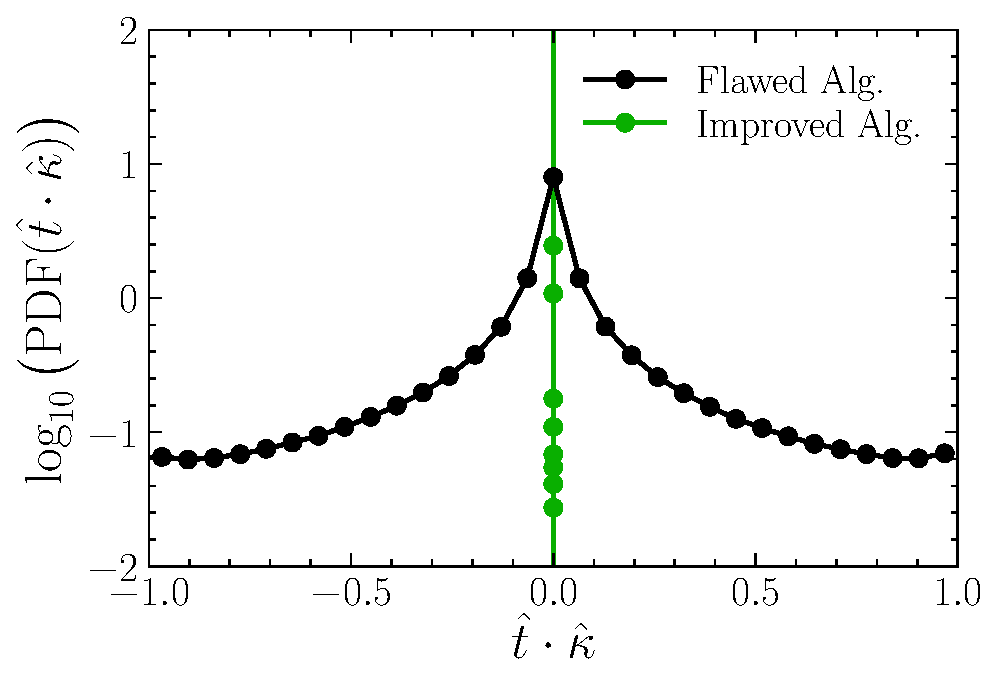
\includegraphics[width=0.65\linewidth]{figures/ssd-exp/kappa_numerical_error_pdf.pdf}
    \caption{Comparison of how well the orthogonality is maintained between the tangent ($\mVectorBase{t}$) and normal ($\mVectorBase{n}$) basis vectors when computed using a straight-forward, but flawed algorithm (plotted in black; see \S\ref{app:kappa:flawed}) versus our improved algorithm (plotted in green; see \S\ref{app:kappa:improved}). The volume weighted PDFs of $\mVectorBase{t}\cdot\mVectorBase{n}$ is shown for the \SimName{0.3}{600}{5} simulation run at $N_\mathrm{res} = 576$, at a snapshot midway through the kinematic phase. Notice that our improved algorithm maintains orthogonality to machine precision.}
    \label{fig:kappa_error}
\end{figure}

    \chapter{The Universal Growth of Small-Scale Dynamos}
\label{chapter:ssd-nl}

\noindent\hfill\parbox{0.815\textwidth}{\raggedleft
This chapter is mildly adapted from:
\textit{Kriel, N., Beattie, J. R., Krumholz, M. R., Schober, J., \& Armstrong, P. J., The universal growth of magnetic energy during the nonlinear phase of subsonic and supersonic small-scale dynamos/, Phys. Rev. E, accepted}
}\par

\section{Chapter Abstract}

    Small-scale dynamos (SSDs) amplify magnetic fields in turbulent plasmas. Theory predicts nonlinear magnetic energy growth $E_\mathrm{mag} \propto t^{p_\mathrm{nl}}$, but this scaling has not been tested across flow regimes. Using a large ensemble of SSD simulations spanning subsonic to supersonic turbulence, we measure linear growth ($p_\mathrm{nl} = 1$) in subsonic flows and quadratic growth ($p_\mathrm{nl} = 2$) in supersonic flows. In all cases, the nonlinear dynamo converts a nearly constant fraction $\sim 1/100$ of the turbulent kinetic energy flux into magnetic energy, and the nonlinear phase has a characteristic duration \DIFdelbegin \DIFdel{$\Delta t \approx 20\,t_0$, where $t_0$ }\DIFdelend \DIFaddbegin \DIFadd{$\Delta t \approx 20\,t_\mathrm{turb}$, where $t_\mathrm{turb}$ }\DIFaddend is the outer-scale turnover time. By isolating the onset of magnetic backreaction in SSDs, our statistical ensemble approach identifies a robust efficiency and duration for the nonlinear SSD that can be used to interpret more complex astrophysical and laboratory plasmas.

\section{Chapter Introduction}

    Small-scale dynamo (SSD) action describes the process by which motions in a plasma with dynamically weak magnetic fields amplify and then maintain the magnetic energy density, $E_\mathrm{mag}$, to levels comparable to the turbulent kinetic energy density, $E_\mathrm{kin}$ \citep{brandenburg2012current, rincon2019dynamo, rempel2023small}. This process is ubiquitous across astrophysical, geophysical, and laboratory environments, both those where the plasma supports turbulent subsonic motions (turbulent sonic Mach number \DIFdelbegin \DIFdel{$\mSonicMach = u_0/c_s < 1$, where $u_0$ }\DIFdelend \DIFaddbegin \DIFadd{$\mSonicMach = u_\mathrm{turb}/c_s < 1$, where $u_\mathrm{turb}$ }\DIFaddend is the rest-frame root-mean-squared velocity and $c_s$ the sound speed) and where they are supersonic ($\mSonicMach > 1$). The fields generated in this process magnetize the plasma between galaxies \citep{Roh2019_galaxy_clusters, tevlin2025magnetic}, provide pressure support against collapse in galaxy mergers \citep{whittingham2021impact}, enable rapid spin-down of stellar merger remnants \citep{palenzuela2022turbulent, ryu2025magnetic}, and modify cosmic ray propagation via curvature acceleration in the interstellar medium (ISM) \DIFdelbegin \DIFdel{\mbox{%DIFAUXCMD
\citep{kempski2023cosmic, Lemoine2023_curvature_accleration}}\hskip0pt%DIFAUXCMD
}\DIFdelend \DIFaddbegin \DIFadd{\mbox{%DIFAUXCMD
\citep{kempski2023cosmic, Lemoine2023_field_reversal_CR_transport}}\hskip0pt%DIFAUXCMD
}\DIFaddend . Direct evidence for SSD action comes both from \textit{in situ} observations in the Earth's subsonic magnetosheath \citep{voros2025turbulent} and from supersonic laboratory laser experiments \citep{Meinecke2014_SSD_lab_Nature, tzeferacos2018laboratory, Bott2021_supersonic_dynamo_in_lab, Bott2021_time_resolved_lab_dynamo}.

    SSDs evolve through a number of distinct phases \citep{moffatt1970dynamo, vainshtein1972origin, kulsrud1992spectrum, schekochihin2002model, schekochihin2004simulations, maron2004nonlinear, rincon2019dynamo}. At first the magnetic field is too weak to exert significant forces on the plasma and thus the velocity field is kinematic, which leads to exponential amplification of the magnetic energy density, $E_\mathrm{mag} \propto \exp(\gamma_\mathrm{exp} t)$. Here $\gamma_\mathrm{exp}$ is the kinematic growth rate (with units of inverse time), and the dimensionless product \DIFdelbegin \DIFdel{$\gamma_\mathrm{exp} t_0$ }\DIFdelend \DIFaddbegin \DIFadd{$\gamma_\mathrm{exp} t_\mathrm{turb}$ }\DIFaddend measures how efficiently kinetic energy is converted into magnetic energy over one outer-scale eddy turnover time \DIFdelbegin \DIFdel{$t_0 = \ell_0/u_0$, where $u_0$ }\DIFdelend \DIFaddbegin \DIFadd{$t_\mathrm{turb} = \ell_\mathrm{turb}/u_\mathrm{turb}$, where $u_\mathrm{turb}$ }\DIFaddend is the flow velocity on the outer scale \DIFdelbegin \DIFdel{$\ell_0$ }\DIFdelend \DIFaddbegin \DIFadd{$\ell_\mathrm{turb}$ }\DIFaddend \citep{moffatt1970dynamo, kulsrud1992spectrum}. For magnetic Prandtl numbers $\mPrm \gtrsim 1$, the dimensionless growth rate is predicted to scale as \DIFdelbegin \DIFdel{$\gamma_\mathrm{exp} t_0 \propto \mReh^{1/2}$ }\DIFdelend \DIFaddbegin \DIFadd{$\gamma_\mathrm{exp} t_\mathrm{turb} \propto \mReh^{1/2}$ }\DIFaddend for $\mSonicMach < 1$ and \DIFdelbegin \DIFdel{$\gamma_\mathrm{exp} t_0 \propto \mReh^{1/3}$ }\DIFdelend \DIFaddbegin \DIFadd{$\gamma_\mathrm{exp} t_\mathrm{turb} \propto \mReh^{1/3}$ }\DIFaddend for $\mSonicMach > 1$, where \DIFdelbegin \DIFdel{$\mReh \sim u_0 \ell_0 / \nu$ }\DIFdelend \DIFaddbegin \DIFadd{$\mReh \sim u_\mathrm{turb} \ell_\mathrm{turb} / \nu$ }\DIFaddend is the hydrodynamic Reynolds number \citep{schober2012magnetic} and $\nu$ is the kinematic viscosity. Field amplification is driven by chaotic stretching \citep{rincon2019dynamo}, which occurs on an eddy turnover timescale $t_\ell \sim \ell/u_\ell$, where $u_\ell$ is the flow speed on size scale $\ell$, and thus is fastest on the viscous scale $\ell_\nu$, which, for Kolmogorov turbulence, is the scale on which eddies evolve on the shortest timescales \citep{bian2019decoupled, brandenburg2019reversed, grete2021matter, kriel2022fundamental, kriel2025fundamental, beattie2025taking}. However, once the kinematic dynamo amplifies the field such that $E_\mathrm{mag} \approx E_\mathrm{kin}$ on scale $\ell_\nu$, the magnetic field begins to back react on the velocity, marking the end of the kinematic phase and the start of the nonlinear phase. During this phase the dominant stretching scale $\ell_s$ shifts to larger $\ell$ with longer $t_\ell$, driving a slower, secular dynamo. As the field grows, it suppresses stretching on ever-larger scales, until $\ell_s$ reaches a maximum scale. At this point the dynamo reaches the saturated phase, and becomes statistically steady, driven MHD turbulence \citep{beattie2025spectrum}.

    Both numerical simulations \citep{schekochihin2004simulations, kriel2022fundamental, kriel2025fundamental}, and laboratory experiments \citep{tzeferacos2018laboratory, Bott2021_supersonic_dynamo_in_lab, Bott2021_time_resolved_lab_dynamo} confirm that the evolution of $E_\mathrm{mag}$ during the kinematic phase agrees well with both the Kazanstev, Anderson \& Kulsrud SSD theory \citep{kazantsev1968, kulsrud1992spectrum} as well as with numerical works in the $\mSonicMach > 1$ regime \citep{Federrath2011_supersonic_dynamo, Federrath2014_supersonic_dynamo, kriel2025fundamental}. However, this well-understood phase likely ends almost immediately in real astrophysical plasmas. This is because the growth rate is \DIFdelbegin \DIFdel{$\gamma_\mathrm{exp} t_0 \propto \mReh^{1/2}$}\DIFdelend \DIFaddbegin \DIFadd{$\gamma_\mathrm{exp} t_\mathrm{turb} \propto \mReh^{1/2}$}\DIFaddend , and many warm or cold astrophysical plasmas, at least in our Galaxy and its surrounding medium, often have $\mReh \sim 10^3-10^{10}$, thus making the kinematic phase persist for only a small fraction of the outer dynamical timescale. Hence, almost any observable astrophysical system where the field is growing will instead be in the nonlinear phase, which is a regime that has not yet been explored with the same level of numerical detail as the kinematic dynamo.

    While there is indication that the nonlinear phase yields secular growth for the magnetic energy \citep{beresnyak2012universal, cho2009growth, seta2020seed, galishnikova2022tearing, kriel2025fundamental}, $E_\mathrm{mag} = \alpha_\mathrm{nl} t^{p_\mathrm{nl}}$, there are no simulations to date that have measured the efficiency $\alpha_\mathrm{nl}$ and growth order $p_\mathrm{nl}$ across a wide range of plasma Reynolds number $\mReh$ and Mach number $\mSonicMach$. For incompressible Kolmogorov-like turbulence, where $E_\mathrm{kin}(\ell) \propto \ell^{5/3}$, the prevailing expectation and hint from numerical simulations is that $p_\mathrm{nl} = 1$ \citep{kulsrud1992spectrum, schekochihin2002model, cho2009growth, beresnyak2012universal, xu2016turbulent}, and $\alpha_\mathrm{nl} \propto \varepsilon$, where $\varepsilon \sim \rho_\ell u_\ell^3/\ell$ is the turbulent energy flux through scale $\ell$, with $\rho_\ell$ the density associated with motions on that scale (which is constant in the incompressible limit). In contrast, for highly-compressible, shock-dominated turbulence, where $E_\mathrm{kin}(\ell) \propto \ell^2$ (as in Burgers-like turbulence \citep{Federrath2013_universality, Federrath2021_the_sonic_scale, kriel2025fundamental, beattie2025taking}), the outcome is debated: some models \citep{schleicher2013small, schober2015saturation} predict quadratic growth ($p_\mathrm{nl} = 2$), while others suggest universal linear growth ($p_\mathrm{nl} = 1$) \citep{beresnyak2012universal}.

    This lack of consensus about the nonlinear growth order $p_\mathrm{nl}$ and efficiency $\alpha_\mathrm{nl}$, particularly in highly-compressible turbulence, is largely due to a dearth of numerical and experimental guidance, which is missing in large part because it is extremely challenging to accurately measure the nonlinear phase. At the modest values of $\mReh$ accessible to numerical simulations and laboratory experiments, the nonlinear phase is hard to identify, due in part to the strong fluctuations of integral quantities that can easily mask underlying trends, especially in supersonic flows. Our goal in this \DIFdelbegin \DIFdel{study, }\DIFdelend \DIFaddbegin \DIFadd{chapter }\DIFaddend is to take on these challenges by focusing on plasmas with $\mPrm = 1$, for which the nonlinear phase we resolve \DIFdelbegin \DIFdel{, }\DIFdelend can only be the backreaction stage that begins once $E_\mathrm{mag} \approx E_\mathrm{kin}$ on the viscous scale. This choice also maximizes the computational dynamic range over which the nonlinear backreaction can operate, because the viscous and resistive dissipation scales for any choice of $\mReh$ or $\mRem$ coincide with one-another ($\ell_\nu \approx \ell_\eta$). Within this setting we directly measure $\alpha_\mathrm{nl}$ and $p_\mathrm{nl}$ across a broad range of plasma parameters (in $\mReh$ and $\mSonicMach$), allowing us, for the first time, to confront theoretical predictions for the backreaction during the nonlinear phase with highly-detailed measurements from simulations. At the same time, our results provide a well-controlled reference point for future studies of more realistic hot astrophysical plasmas with $\mPrm \gg 1$, where this backreaction stage may be preceded by an additional nonlinear, secular growth phase in the sub-viscous range (see the discussion in the Conclusion).

\section{Numerical Methods}

\subsection{Numerical Simulations} \label{sec:methods:sims}

    \begin{figure}
        \centering
        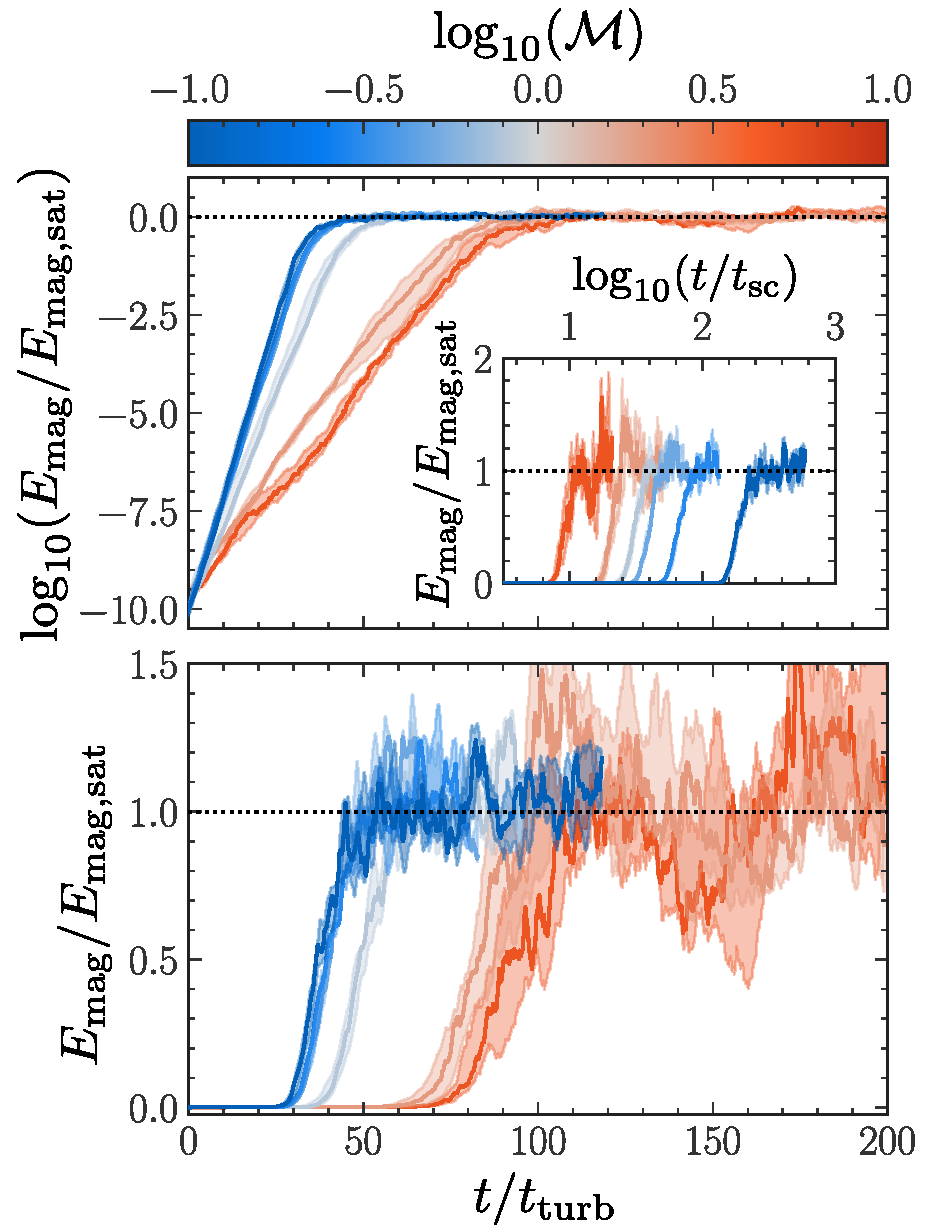
\includegraphics[width=0.65\linewidth]{figures/ssd-nl/time_evolution.pdf}
        \caption{Time evolution of the volume-averaged magnetic energy $E_\mathrm{mag}$, normalized by the final saturated value $E_{\mathrm{mag},\mathrm{sat}}$, for a subset of SSD simulations with $\mReh = 1500$. The top panel shows the energy in logarithmic scale, and the bottom panel (and inset) shows it in linear scale. Each simulation configuration is repeated five times with independent random seeds for the turbulent forcing; we plot the median trend across realizations as a solid line, with the 16th to 84th percentile range indicated by a shaded band. Colors indicate the average sonic Mach number $\mSonicMach$ of each configuration. In the main axes, time is shown in units of the turbulent turnover time on the outer scale, \DIFdelbeginFL \DIFdelFL{$t_0$}\DIFdelendFL \DIFaddbeginFL \DIFaddFL{$t_\mathrm{turb}$}\DIFaddendFL , and rescaled to the sound-crossing time, $t_\mathrm{sc}$, in the inset.}
        \label{fig:time_series}
    \end{figure}

    We used a modified version of the \textsc{flash} code \citep{Fryxell2000, Dubey2008, Waagan2011, Federrath2021_the_sonic_scale} to run a series of direct numerical simulations that solve the compressible, non-ideal MHD equations for an isothermal plasma in a three-dimensional periodic box \citep{kriel2025fundamental}; the full set of equations we solve is provided in End Matter \DIFaddbegin \DIFadd{(\S\ref{app:ssd-nl:simulation-setup})}\DIFaddend . We work in dimensionless units where the box size $L$, mean density $\rho_0$, $c_s$, and mean thermal energy $\rho_0 c_s^2$ are unity. The natural unit of time for this system is the sound-crossing time, $t_\mathrm{sc} = L / c_\mathrm{s} = 1$, and the turbulent velocity \DIFdelbegin \DIFdel{$u_0$ }\DIFdelend \DIFaddbegin \DIFadd{$u_\mathrm{turb}$ }\DIFaddend directly sets the sonic Mach number, \DIFdelbegin \DIFdel{$\mSonicMach = u_0/c_s$}\DIFdelend \DIFaddbegin \DIFadd{$\mSonicMach = u_\mathrm{turb}/c_s$}\DIFaddend . By varying \DIFdelbegin \DIFdel{$u_0$}\DIFdelend \DIFaddbegin \DIFadd{$u_\mathrm{turb}$}\DIFaddend , we control the speed of the flow relative to $t_\mathrm{sc}$, and in turn can explore subsonic (\DIFdelbegin \DIFdel{$t_\mathrm{sc} < t_0$}\DIFdelend \DIFaddbegin \DIFadd{$t_\mathrm{sc} < t_\mathrm{turb}$}\DIFaddend ) and supersonic (\DIFdelbegin \DIFdel{$t_0 < t_\mathrm{sc}$}\DIFdelend \DIFaddbegin \DIFadd{$t_\mathrm{turb} < t_\mathrm{sc}$}\DIFaddend ) regimes. We use the \textsc{turbgen} \citep{Federrath2022_TurbGen} forcing-module to drive purely-solenoidal ($\mVector{\nabla}\cdot\mVector{f}=0$) turbulence with momentum source term $\mVector{f}$, following the standard protocol outlined in \citet{kriel2022fundamental}, allowing us to set $\mSonicMach \in [5\times 10^{-2}, 5]$\DIFdelbegin \DIFdel{(}\DIFdelend \DIFaddbegin \DIFadd{; }\DIFaddend see End Matter \DIFaddbegin \DIFadd{(\S\ref{app:ssd-nl:simulation-setup}) }\DIFaddend for more details\DIFdelbegin \DIFdel{)}\DIFdelend .

    By varying the (constant in space and time) kinematic viscosity coefficient, $\nu$, across different simulation configurations, we explore a range of hydrodynamic Reynolds numbers, $\mReh \in [10^3, 5\times 10^3]$, where we set the magnetic Prandtl number $\mPrm \equiv \nu/\eta = \mRem/\mReh = 1$; $\eta$ is the magnetic resistivity coefficient and $\mRem$ is the magnetic Reynolds number. We quote $\mReh$ and $\mRem$ using \DIFdelbegin \DIFdel{$u_0$}\DIFdelend \DIFaddbegin \DIFadd{$u_\mathrm{turb}$}\DIFaddend , which is the rest-frame root-mean-squared velocity measured in the statistically steady kinematic phase. For convenience, we use these kinematic values to label simulations and compare across the parameter space. During the nonlinear and saturated phases, magnetic backreaction slightly suppresses the velocity amplitude, so the instantaneous effective values of $\mReh$ and $\mRem$ may be smaller than their nominal kinematic values. This effect, however, is minor for $\mPrm = 1$, becoming more prominent for $\mPrm \gg 1$ \citep{seta2021saturation, shivakumar2025numerical}. Because $\mReh = \mRem \gtrsim \mRem_\mathrm{crit} \approx 100$, all simulations are above the critical $\mRem$ required to undergo all phases of the SSD \citep{schekochihin2007fluctuation, schober2015saturation, Seta2020_critical_Rm}. In total we consider $12$ distinct (but over many different statistical realizations of $\mVector{f}$, detailed in the next paragraph) combinations of $\mSonicMach$ and $\mReh$ -- see End Matter \DIFaddbegin \DIFadd{(\S\ref{app:ssd-nl:simulation-setup}) }\DIFaddend for a complete list of simulations. We also ran pilot simulations at lower $\mReh$, but found that the volume-integrated kinetic and magnetic energies had relative fluctuations that were too large for our analysis. When the viscous and resistive dissipation scales $\ell_\nu$ and $\ell_\eta$ lie close to the forcing scale \DIFdelbegin \DIFdel{$\ell_0$}\DIFdelend \DIFaddbegin \DIFadd{$\ell_\mathrm{turb}$}\DIFaddend , the cascade is truncated and fluctuations remain confined to large scales. The effective number of independent eddies contributing to volume averages, $N_{\rm eddies} \sim (L/\ell_\nu)^3$, is then small, so the fractional fluctuations $\propto N_{\rm eddies}^{-1/2}$ remain large in the nonlinear phase. For this reason we adopt moderately turbulent flows with $\mReh \gtrsim 10^3$ as our practical lower bound. Finally, we caution readers that there are two different conventions in use in the literature to define the Reynolds number; our definition, \DIFdelbegin \DIFdel{$\mReh \sim u_0 \ell_0 / \nu$}\DIFdelend \DIFaddbegin \DIFadd{$\mReh \sim u_\mathrm{turb} \ell_\mathrm{turb} / \nu$}\DIFaddend , is a factor of $2\pi$ larger than that used by some authors \citep[\eg][]{brandenburg2023dissipative, galishnikova2022tearing}, so in the convention used by these authors, our simulations span $\mReh \in [1.5\times 10^2, 8\times 10^2]$.

    In all our simulations we initialize a weak seed magnetic field $E_{\mathrm{mag}, 0} \equiv E_\mathrm{mag}(t=0) = 10^{-10} E_\mathrm{kin}$, where $E_\mathrm{kin}$ is the kinetic energy once turbulence is fully established in the kinematic phase. We evolve each simulation instance long enough to unambiguously identify the onset and transition out of the nonlinear phase (see next section). To reduce the impact of fluctuations during the nonlinear phase on our fit parameters, we repeat each configuration at least five times with different random seeds for $\mVector{f}$. We perform runs at three resolutions, $N_\mathrm{res} \in \{288^3, 576^3, 1152^3\}$, and run a total of $89$ independent simulation instances. We plot the time evolution for the integral magnetic field energy of a representative subset of our simulations ($\mSonicMach$-varied with $\mReh = 1500$) in Fig.~\ref{fig:time_series}, where the classical SSD phases are clear to see. The main panels use \DIFdelbegin \DIFdel{$t_0$ }\DIFdelend \DIFaddbegin \DIFadd{$t_\mathrm{turb}$ }\DIFaddend to emphasize the evolution in outer-scale turnover times, while the inset re-normalizes the same curves in units of the sound-crossing time $t_\mathrm{sc}$, highlighting how the ordering of the nonlinear phase onset changes when measured against $t_\mathrm{sc}$ rather than \DIFdelbegin \DIFdel{$t_0$}\DIFdelend \DIFaddbegin \DIFadd{$t_\mathrm{turb}$}\DIFaddend .

\subsection{Fitting Procedure} \label{sec:methods:fitting}

    To constrain growth timescales during the nonlinear phase, we begin by binning the raw time series of volume-averaged magnetic energy density $E_\mathrm{mag}$, for each of our simulations, into intervals of \DIFdelbegin \DIFdel{$t_0$}\DIFdelend \DIFaddbegin \DIFadd{$t_\mathrm{turb}$}\DIFaddend . Within each time bin $t_i$, we compute the mean $\mu_i$ and standard deviation $\sigma_i$ of both $E_\mathrm{mag}$ and $\ln(E_\mathrm{mag})$ in bin $i$; $\mu_i^{(\ln)}$ and $\sigma_i^{(\ln)}$ indicate the mean and standard deviation of $\ln(E_\mathrm{mag})$ in bin $i$. This yields, for each simulation $j$, a dataset $\mVector{\mathcal{D}}_j \equiv (t_i, \mu_i, \mu_i^{(\ln)}, \sigma_{i}, \sigma_i^{(\ln)})$, where data points are (approximately) uncorrelated, given that the turbulence correlation time is \DIFdelbegin \DIFdel{$t_0$}\DIFdelend \DIFaddbegin \DIFadd{$t_\mathrm{turb}$}\DIFaddend .

    Using a hierarchical two-stage strategy, we then employ a Bayesian approach to fit each $\mVector{\mathcal{D}}_j$ to models for the time evolution of magnetic energy. In the first stage we only constrain the exponential and saturated behavior, and in the second stage we fit the full three-phase model with priors informed by the first. This ensures that the more complex nonlinear-phase dynamics remain stable and well-constrained, especially in our supersonic simulations, where large fluctuations can make the nonlinear phase difficult to identify. Anchoring in this way also improves the sampling efficiency.

    Our first stage models only the kinematic and saturated phases, approximating the transition between these phases as instantaneous,
    \begin{align}
        f_1(t \mid \mVector{\theta}_1) =
            \begin{cases}
                E_0 \exp(\gamma_\mathrm{exp} t) , & t < t_\mathrm{sat} \\
                E_0 \exp(\gamma_\mathrm{exp} t_\mathrm{sat}) , & t \geq t_\mathrm{sat}
            \end{cases}
    \end{align}
    with $\mVector{\theta}_1 = (E_0, \gamma_\mathrm{exp}, t_\mathrm{sat})$, and the second stage models all dynamo phases self-consistently as
    \begin{align}
        f_2(t \mid \mVector{\theta}_2) =
            \begin{cases}
                E_0 \exp(\gamma_\mathrm{exp} t) , &
                    t < t_\mathrm{nl} \\
                E_0 \exp(\gamma_\mathrm{exp} t_\mathrm{nl})
                    + \alpha_\mathrm{nl} (t - t_\mathrm{nl})^{p_\mathrm{nl}} , & t_\mathrm{nl} \leq t < t_\mathrm{sat} \\
                E_\mathrm{sat} , &
                    t \geq t_\mathrm{sat}
            \end{cases} \label{eqn:integral_energy_model}
    \end{align}
    where $\mVector{\theta}_2 = (E_0, E_\mathrm{sat}, \gamma_\mathrm{exp}, t_\mathrm{nl}, t_\mathrm{sat}, p_\mathrm{nl})$. Here, $\alpha_\mathrm{nl}$ is not a fit parameter in the second stage, because it is implicitly set by the requirement that $f_2$ must remain continuous at $t = t_\mathrm{sat}$.

    \begin{figure}
        \centering
        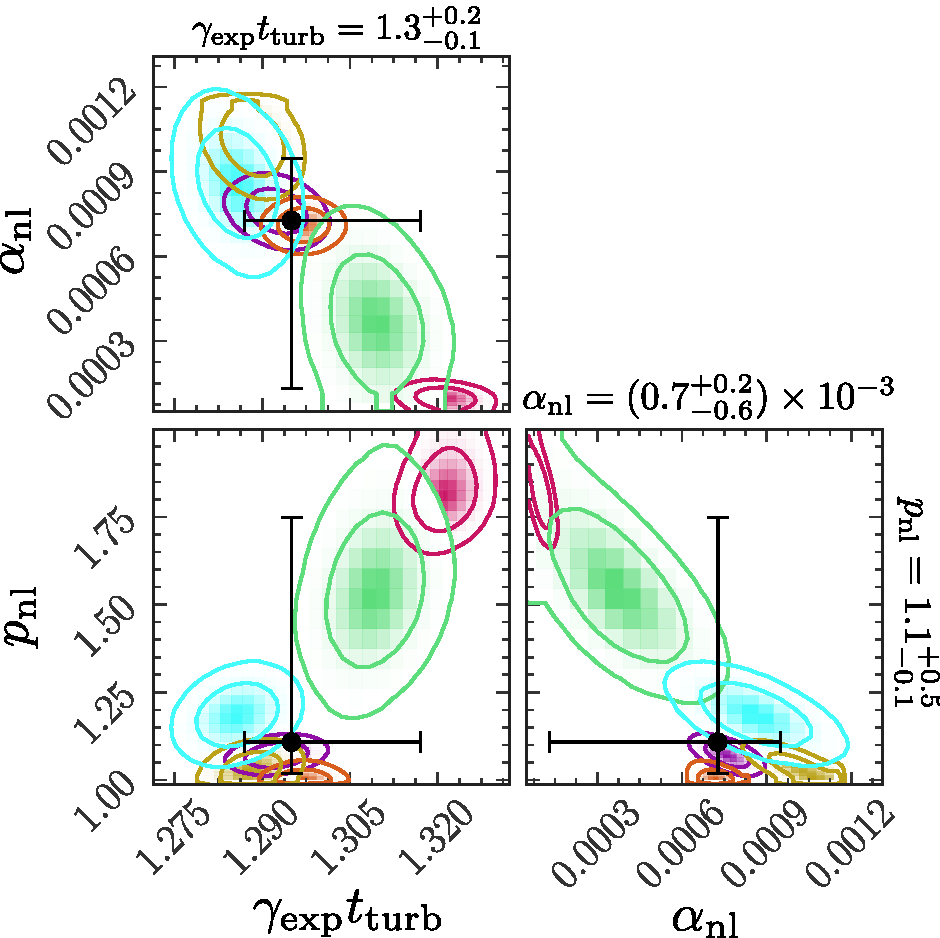
\includegraphics[width=0.75\linewidth]{figures/ssd-nl/posteriors.pdf}
        \caption{Joint posterior distributions for three key parameters (from Eqn.~\ref{eqn:integral_energy_model}) describing the evolution of magnetic energy, inferred from the six independent realizations of the $\mSonicMach = 0.5$, $\mReh = 1500$ simulation at $N_\mathrm{res} = 576^3$. Panels show the correlations between the dimensionless kinematic growth rate \DIFdelbeginFL \DIFdelFL{$\gamma_\mathrm{exp} t_0$}\DIFdelendFL \DIFaddbeginFL \DIFaddFL{$\gamma_\mathrm{exp} t_\mathrm{turb}$}\DIFaddendFL , the nonlinear growth coefficient $\alpha_\mathrm{nl}$, and the nonlinear growth exponent $p_\mathrm{nl}$. Colored contours show (one color per realization) the posteriors inferred for each individual realization using the fitting procedure described in Section~\ref{sec:methods:fitting}. The black marker with error bars indicates the aggregated posterior inferred by combining samples from all six realizations with equal weight, plotted as the median and 16th--84th percentile range for each parameter.}
        \label{fig:posterioirs}
    \end{figure}

    For our fits in both stages, we assume that each data point $d_i$ in the time series is an independent sample from a Gaussian distribution around a mean trend, so for any given time series of simulation data $\mVector{\mathcal{D}}_j$, the log likelihood function is
    \begin{align}
        \ln \mathcal{L}(\mVector{\theta}_s \mid \mVector{\mathcal{D}}_j)
            = -\frac{1}{2} \sum_{i} \sbrac{
                \frac{ \left( d_i - f_s(t_i \mid \mVector{\theta}_s)\right)^2 }{ e_i^2 }
            } ,
    \end{align}
    where we fit $(d_i, e_i) = (\mu_i^{(\ln)}, \sigma_i^{(\ln)})$ in stage one ($s = 1$), and we fit $(d_i, e_i) = (\mu_i, \sigma_i)$ in stage two ($s = 2$). This is because, as is apparent from Fig.~\ref{fig:time_series}, it is much easier to identify the kinematic (exponential growing) phase in logarithmic space, and the nonlinear (backreaction) phase in linear space.

    We fit using a Markov Chain Monte Carlo method \cite{Foreman-Mackey13a}; see End Matter \DIFaddbegin \DIFadd{(\S\ref{app:ssd-nl:mcmc}) }\DIFaddend for details on our sampling parameters. In the first stage we adopt uniform (unbiased) priors on $\gamma_\mathrm{exp} \in (0, 10]$ and $t_\mathrm{sat} \in (0, t_\mathrm{end})$, where $t_\mathrm{end}$ is the final time bin, and a log-uniform prior on $E_0 \in [10^{-30}, 10^{-5}]$ (due to its wide dynamic range). In the second stage, the \textit{priors} for $E_0$, $\gamma_\mathrm{exp}$ and $E_\mathrm{sat}$ are taken to be the \textit{posteriors} from stage one. We assign a uniform prior $p_\mathrm{nl} \in [1,2]$, consistent with existing theories, while, for $t_\mathrm{nl}$ and $t_\mathrm{sat}$ we use priors that are uniform on the intervals $[0,t_{\mathrm{nl}, \mathrm{max}}]$ and $[t_\mathrm{nl},t_{\mathrm{sat},\mathrm{max}}]$, where $t_{\mathrm{nl}, \mathrm{max}}$ is the time bin where $dE_\mathrm{mag}/dt$ is its maximum, and $t_{\mathrm{sat},\mathrm{max}}$ is the earliest time $t_i$ for which $dE_\mathrm{mag}/dt < 0$.

    After fitting each individual simulation, we aggregate posteriors across runs with the same resolution and plasma parameters. This is the key step in our procedure, where we average out the inevitably large fluctuations in any single realization. This is illustrated in Fig.~\ref{fig:posterioirs} for our set of six independent realizations of the $\mSonicMach = 0.5$, $\mReh = 1500$ simulation at $N_\mathrm{res} = 576^3$. For any given configuration, then, all realizations are statistically equivalent and differ only in their random driving, so we combine their posterior samples with equal weighting. Fitting each simulation separately preserves the phase structure of each realization, while still averaging over ensemble variability. This is crucial, because identical realizations may enter the nonlinear and saturated phases at slightly different times relative to one another. Accurately constraining these transition times is essential for robustly measuring the nonlinear growth dynamics, which would be averaged out if all instances of a configuration were fit simultaneously. All the results we present in the remainder of this \DIFdelbegin \DIFdel{study }\DIFdelend \DIFaddbegin \DIFadd{chapter }\DIFaddend are derived from these aggregated samples; percentiles of these derived quantities are reported in Table~\ref{table:ssd-nl:summary}, and the raw data, along with our implementation of the routines discussed here, are publicly available online \citep{mydata}.

\section{Chapter Results}

\subsection{Kinematic dynamo growth}

    \begin{figure}
        \centering
        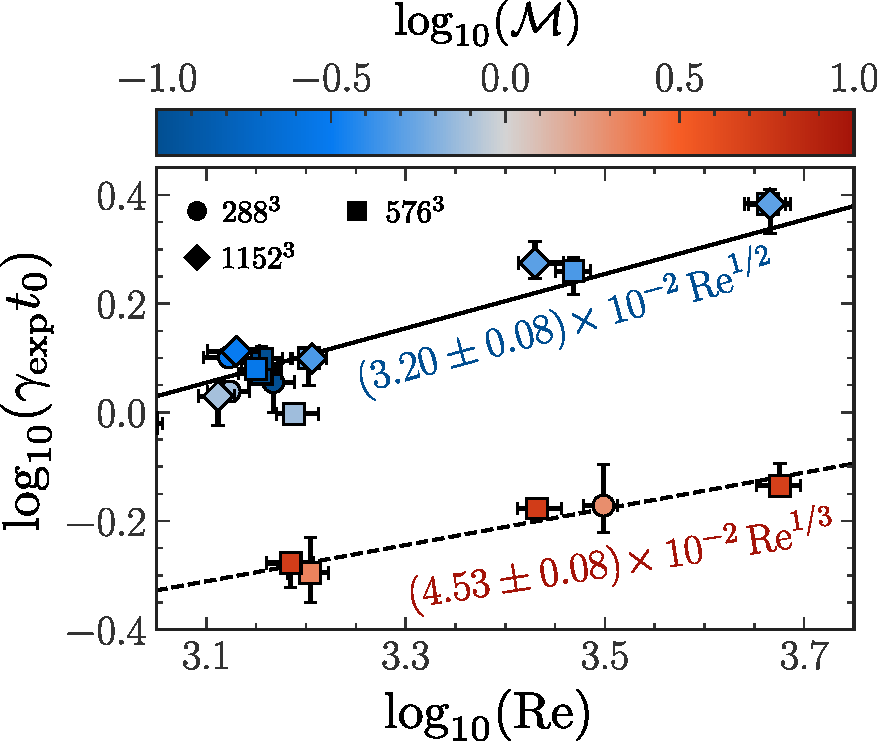
\includegraphics[width=0.65\linewidth]{figures/ssd-nl/gamma_exp_scaling.pdf}
        \caption{Kinematic growth rates, $\gamma_\mathrm{exp}$, as a function of plasma Reynolds number, $\mReh$, with markers indicating different $N_\mathrm{res}$, and colors showing $\mSonicMach$. Each data point shows the median marginal posterior probability for $\gamma_\mathrm{exp}$ derived by fitting Eqn.~\ref{eqn:integral_energy_model} to each plasma combination, $(N_\mathrm{res},\mSonicMach,\mReh)$. The vertical error bars show the 16th to 84th percentile range from the fits and the horizontal error bars show the same for the fluctuations measure in \DIFdelbeginFL \DIFdelFL{$\mReh = u_0 \ell_0/\nu$ }\DIFdelendFL \DIFaddbeginFL \DIFaddFL{$\mReh = u_\mathrm{turb} \ell_\mathrm{turb}/\nu$ }\DIFaddendFL over time. Lines show fits of $\gamma_\mathrm{exp} \propto \mReh^{1/2}$ to subsonic points (solid line) and $\gamma_\mathrm{exp} \propto \mReh^{1/3}$ to supersonic points (dashed line), which match predictions from \cite{schober2012small, schober2012magnetic}, indicating that the viscous scale is the engine for growth in the kinematic regime.}
        \label{fig:gamma_exp_scaling}
    \end{figure}

    In Fig.~\ref{fig:gamma_exp_scaling} we show our inferred kinematic-phase growth rates, \DIFdelbegin \DIFdel{$\gamma_\mathrm{exp} t_0$}\DIFdelend \DIFaddbegin \DIFadd{$\gamma_\mathrm{exp} t_\mathrm{turb}$}\DIFaddend , for each plasma configuration. Consistent with both theoretical expectation and prior work, we find that the data follow $\gamma_\mathrm{exp} \propto \mReh^{1/2}$ for $\mSonicMach \lesssim 1$ and $\gamma_\mathrm{exp} \propto \mReh^{1/3}$ for $\mSonicMach > 1$ simulations. Both scalings align with the expectation that magnetic growth is regulated by the stretching on the viscous scale of the hydrodynamical cascade, $\gamma_\mathrm{exp} \sim u_\nu/\ell_\nu \sim \mReh^{(1-\vartheta)/(1+\vartheta)}$, with $\vartheta = 1/2$ for Kolmogorov-like, and $\vartheta = 1/3$ for Burgers-like turbulence \citep{kulsrud1992spectrum, schekochihin2002model, schober2012magnetic}. We find that the growth rate transitions sharply between the two regimes, \ie as soon as the turbulence becomes even mildly supersonic the growth rate follows $\gamma_\mathrm{exp} \propto \mReh^{1/3}$.

    While the scaling of $\gamma_\mathrm{exp}$ with $\mReh$ in our simulations is in agreement with theoretical expectations, the proportionality constants we measure, of order $\sim 1/100$, are systematically smaller than expected. A simple least-squares fit of the dimensionless kinematic growth rate, \DIFdelbegin \DIFdel{$\gamma_\mathrm{exp} t_0$}\DIFdelend \DIFaddbegin \DIFadd{$\gamma_\mathrm{exp} t_\mathrm{turb}$}\DIFaddend , as a function of $\mReh$, gives $(3.22 \pm 0.06) \times 10^{-2} \,\mReh^{1/2}$ for our $\mSonicMach \lesssim 1$ simulations, and $(4.48 \pm 0.06) \times 10^{-2} \,\mReh^{1/3}$ for our $\mSonicMach > 1$ simulations. These fits indicate that the kinematic dynamo only converts $\sim 1/100$ of the hydrodynamical energy flux, $\varepsilon$, into magnetic energy. We show in the next section that this same conversion efficiency also holds in the nonlinear dynamo phase. These values are significantly smaller than predicted for $\mPrm \gg 1$ flows ($37/36$ for Kolmogorov flows, and $11/60$ for Burgers \citep{schober2012small, schober2012magnetic}) and instead align more closely with predictions for $\mPrm \ll 1$ flows, where $0.03$ is expected for Kolmogorov, and $5\times10^{-3}$ for Burgers \citep{schober2012small, schober2012magnetic, bovino2013turbulent}.

\subsection{Nonlinear dynamo growth}

    Fig.~\ref{fig:nl_exponent} shows our measured growth-exponent, $p_\mathrm{nl}$, for $E_\mathrm{mag}$ during the nonlinear phase, and Fig.~\ref{fig:nl_scalings} shows both the growth-efficiency coefficient, $\alpha_\mathrm{nl}$, in the top panel, and duration, $t_\mathrm{sat} - t_\mathrm{nl}$, of the nonlinear phase in the bottom panel. For our $\mSonicMach \lesssim 1$ simulations, we find that growth is close to linear-in-time, $p_\mathrm{nl} \approx 1$, and a least-squares fit to the median results shows that the growth coefficient is $\alpha_\mathrm{nl} = (9.4 \pm 0.7) \times 10^{-3} \mSonicMach^3 \approx 5\times 10^{-3}\varepsilon$, where \DIFdelbegin \DIFdel{$\varepsilon \sim u_0^3 /\ell_0 = 2 \mSonicMach^3$ }\DIFdelend \DIFaddbegin \DIFadd{$\varepsilon \sim u_\mathrm{turb}^3 /\ell_\mathrm{turb} = 2 \mSonicMach^3$ }\DIFaddend is the hydrodynamic energy flux in our simulations. Critically, the growth rate is independent of $\mReh$, suggesting that, even though we have explored only a finite range $\mReh \in [10^3, 5\times 10^3]$, the results are likely to be valid for all turbulent flows (where $\mReh > \mReh_\mathrm{crit} \approx 100$; see \citet{kriel2022fundamental}). This is qualitatively consistent with previous works that have shown only a small, fixed fraction of $\varepsilon$ is converted into magnetic energy \citep{cho2009growth, beresnyak2012universal}, but it has never been measured with this accuracy and precision, across a broad range of plasma parameters. By comparison, \citet{beresnyak2012universal} measured $\alpha_\mathrm{nl} /\varepsilon \approx 0.05$ (compared to our $9.4 \pm 0.7 \times 10^{-3} \sim 10^{-2}$) from ensemble averaged $\mSonicMach \ll 1$, $\mPrm = 1$ simulations, and \citet{xu2016turbulent} predicted $\alpha_\mathrm{nl} /\varepsilon = 3/38$ for $\mSonicMach \ll 1$, $\mPrm \gg 1$ SSDs. We show both of these predictions in Fig.~\ref{fig:nl_scalings}, and while our measured efficiency is a factor of $\approx 10$ lower than both predictions, as was also the case for the growth rate measured during the kinematic phase, the difference, at least compared with \citet{xu2016turbulent}, can be explained by our finite $\mPrm = 1$ simulations. Regardless, the overall results are consistent with the phenomenology of inefficient conversion of turbulent to magnetic energy in the nonlinear phase.

    \begin{figure}
        \centering
        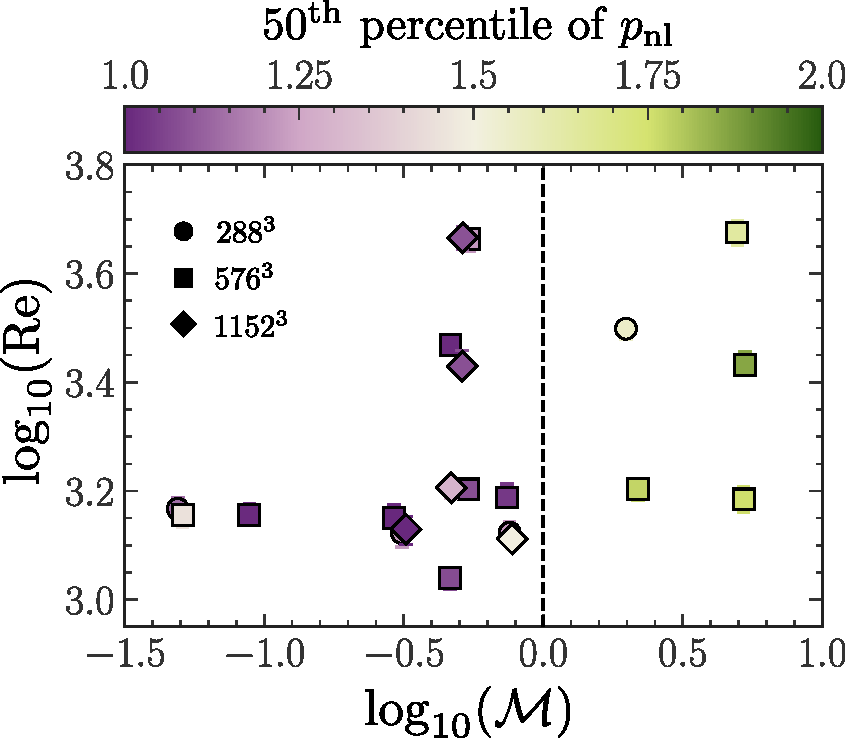
\includegraphics[width=0.65\linewidth]{figures/ssd-nl/nl_exponent.pdf}
        \caption{Secular dynamo growth exponent $p_\mathrm{nl}$, measured during the nonlinear phase, as a function of $\mSonicMach$ and $\mReh$ for each plasma configuration. For $\mSonicMach \lesssim 1$ simulations we unanimously recover linear growth ($p_\mathrm{nl} \approx 1$; purple), and quadratic growth ($p_\mathrm{nl} \approx 2$; green) for all $\mSonicMach > 1$ simulations.}
        \label{fig:nl_exponent}
    \end{figure}

    \DIFaddbegin \clearpage
    \DIFaddend All of our $\mSonicMach > 1$ simulations yield $p_\mathrm{nl} \approx 2$, consistent with quadratic-in-time growth \footnote{A complementary model-comparison analysis\DIFdelbegin \DIFdel{(see }\DIFdelend \DIFaddbegin \DIFadd{, described in }\DIFaddend End Matter \DIFaddbegin \DIFadd{(\S\ref{app:ssd-nl:aic}}\DIFaddend )\DIFaddbegin \DIFadd{, }\DIFaddend confirms that subsonic results are best described by linear growth, while quadratic growth captures the supersonic regime.} of $E_\mathrm{mag}$, aligned with the model of \citet{schleicher2013small}, which predicts that \DIFdelbegin \DIFdel{$E_\mathrm{mag}(t) \sim E_\mathrm{kin}^{1/2} (t/t_0)^2$ }\DIFdelend \DIFaddbegin \DIFadd{$E_\mathrm{mag}(t) \sim E_\mathrm{kin}^{1/2} (t/t_\mathrm{turb})^2$ }\DIFaddend for Burgers-like turbulence. Indeed, as predicted by \citet{schleicher2013small}, this breaks the universality of $p_\mathrm{nl}$ across different $\mSonicMach$ regimes. Moreover, unlike the subsonic case, $\varepsilon$ no longer scales with $\mSonicMach^3$, but instead follows a shallower trend $\alpha_\mathrm{nl} \propto \varepsilon \propto \mSonicMach^2$. Empirically, the trends we measure can be understood if the conversion of $E_{\mathrm{kin}}$ into $E_{\mathrm{mag}}$ is modified by the presence of acoustic modes and shocks, \ie if the flux is transferred on $t_\mathrm{sc}$ timescales, due to a fraction of the energy being directly deposited into shock heating, $\varepsilon \sim u^2/t_{\mathrm{sc}} \sim u^2 c_s / \ell \sim \mSonicMach^2$, which acts to reduce the available hydrodynamical flux by a factor of $\mSonicMach^{-1}$. This is consistent with the idea that in the compressible regime, some fraction of the $E_{\mathrm{kin}}$ fills compressible mode degrees of freedom, which do not contribute to irreversible field amplification \citep{Federrath2011_supersonic_dynamo, Federrath2014_supersonic_dynamo, seta2021saturation, sur2024role, beattie2025taking}.

    \begin{figure}
        \centering
        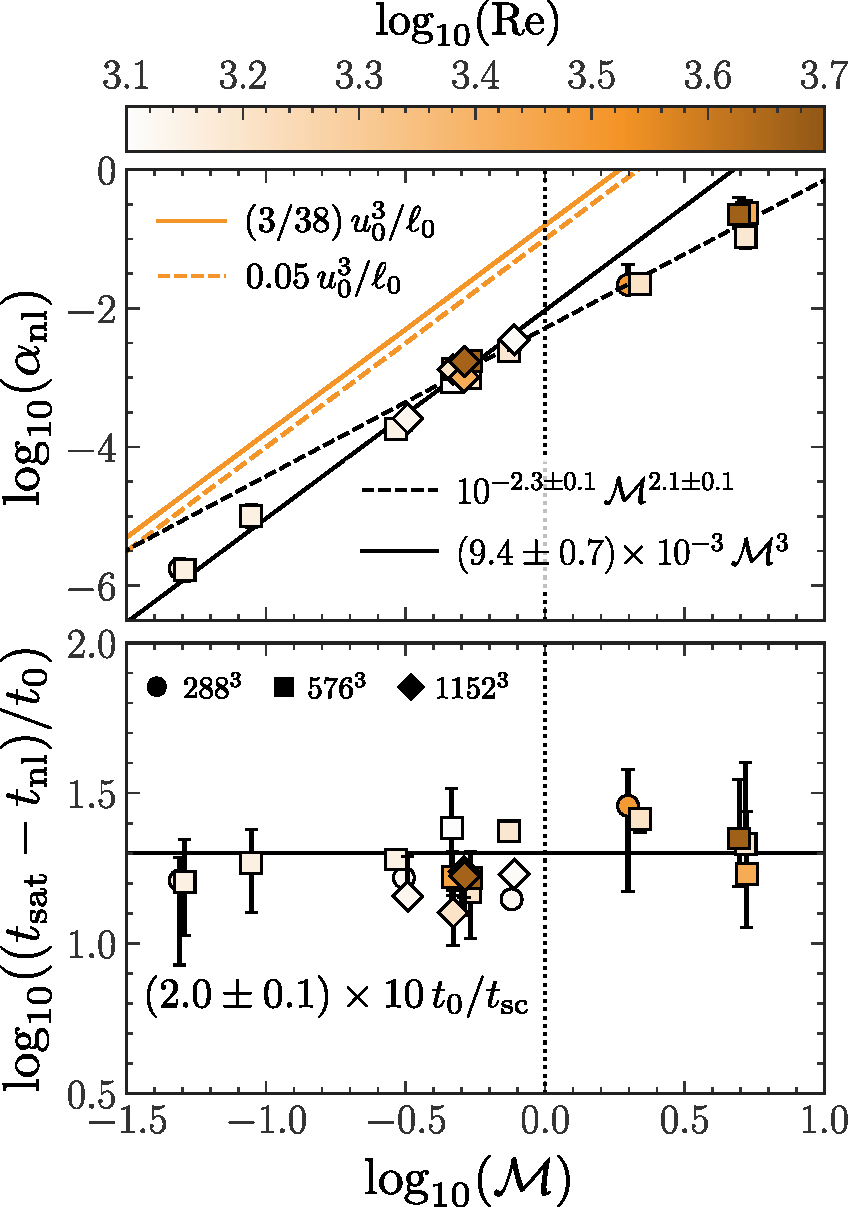
\includegraphics[width=0.65\linewidth]{figures/ssd-nl/nl_scalings.pdf}
        \caption{Nonlinear growth coefficient $\alpha_\mathrm{nl}$ (top panel) and duration of the nonlinear phase normalized by \DIFdelbeginFL \DIFdelFL{$t_0$ }\DIFdelendFL \DIFaddbeginFL \DIFaddFL{$t_\mathrm{turb}$ }\DIFaddendFL (bottom panel), as a function of $\mSonicMach$, and colored by $\mReh$. Points show median posterior values as derived from the MCMC, while error bars show the 16th to 84th percentile range, although in some cases the error bars are not visible because they are smaller than the plot markers. For $\mSonicMach \lesssim 1$ we find $\alpha_\mathrm{nl} \propto \mSonicMach^3$ (black solid line), consistent with turbulent energy-flux-regulated models of nonlinear growth: \DIFdelbeginFL \DIFdelFL{$0.05 u_0^3/\ell_0$ }\DIFdelendFL \DIFaddbeginFL \DIFaddFL{$0.05 u_\mathrm{turb}^3/\ell_\mathrm{turb}$ }\DIFaddendFL from \citep{beresnyak2012universal} (dot-dashed orange) and \DIFdelbeginFL \DIFdelFL{$(3/38)u_0^3/\ell_0$ }\DIFdelendFL \DIFaddbeginFL \DIFaddFL{$(3/38)u_\mathrm{turb}^3/\ell_\mathrm{turb}$ }\DIFaddendFL from \citep{xu2016turbulent} (dotted orange). By contrast, for $\mSonicMach > 1$, we find $\alpha_\mathrm{nl} \propto \mSonicMach^2$ (black dashed), which is shallower than the flux-regulated prediction. Critically, $\alpha_\mathrm{nl}$ in both $\mSonicMach$-regimes becomes independent of $\mReh$, and the cascade itself becomes the dynamo engine, where we find that only a roughly constant fraction of the turbulent kinetic energy flux is converted into magnetic energy, \viz $(dE_\mathrm{mag}/dt)/\varepsilon \approx 1/100$. Across all simulations the nonlinear phase persists for a universal \DIFdelbeginFL \DIFdelFL{$t_\mathrm{sat} - t_\mathrm{nl} \approx 20 t_0$ }\DIFdelendFL \DIFaddbeginFL \DIFaddFL{$t_\mathrm{sat} - t_\mathrm{nl} \approx 20 t_\mathrm{turb}$ }\DIFaddendFL (solid black line in lower panel) duration, invariant to all plasma parameters explored in this \DIFdelbeginFL \DIFdelFL{study}\DIFdelendFL \DIFaddbeginFL \DIFaddFL{chapter}\DIFaddendFL .}
        \label{fig:nl_scalings}
    \end{figure}

    Despite the differences in scaling and $\mSonicMach$-dependence between the $\mSonicMach \lesssim 1$ and $\mSonicMach > 1$ regimes, we find two aspects of the nonlinear SSD that are universal across plasma parameters and $\mSonicMach$-regimes: firstly, the proportionality coefficient, which is associated with the nonlinear SSD efficiency, is universal across all $\mSonicMach$ and $\mReh$, with $\varepsilon / 100$ efficiency consistent with what was found previously \citep{beresnyak2012universal}, even though $p_\mathrm{nl}$ is not always unity. And secondly, across the full parameter space, we find that the nonlinear phase persists for \DIFdelbegin \DIFdel{$t_\mathrm{sat} - t_\mathrm{nl} \approx (20 \pm 1) \,t_0$}\DIFdelend \DIFaddbegin \DIFadd{$t_\mathrm{sat} - t_\mathrm{nl} \approx (20 \pm 1) \,t_\mathrm{turb}$}\DIFaddend , independent of $\mSonicMach$ or $\mReh$ (see Fig.~\ref{fig:nl_scalings}, bottom panel), making the duration in the nonlinear dynamo also universal. This suggests that once the nonlinear phase begins, $E_\mathrm{mag} \approx E_{\mathrm{kin}}(\ell_\nu)$, the system saturates after \DIFdelbegin \DIFdel{$\approx 20 t_0$}\DIFdelend \DIFaddbegin \DIFadd{$\approx 20 t_\mathrm{turb}$}\DIFaddend , regardless of flow compressibility. This universal nonlinear window is visually apparent in both the bottom and inset panels of Fig.~\ref{fig:time_series}, where the nonlinear phase occupies a comparable interval when time is expressed as \DIFdelbegin \DIFdel{$t/t_0$ }\DIFdelend \DIFaddbegin \DIFadd{$t/t_\mathrm{turb}$ }\DIFaddend or $\log_{10}(t/t_\mathrm{sc})$. This is likely because, although $\varepsilon$ and $\alpha_\mathrm{nl}$ have different $\mSonicMach$-dependencies, their ratio remains $\alpha_\mathrm{nl} / \varepsilon \approx 1/100$ for all dynamo (both kinematic and nonlinear) and flow regimes (sub- and supersonic) (Fig.~\ref{fig:nl_scalings}, top panel). The implication is that while the algebraic order and $\mSonicMach$ dependence of $E_\mathrm{mag}$ growth depends on the turbulent regime, the path to saturation is set by a robust and universal dynamical clock.

\section{Chapter Discussion and Conclusions}

    In this \DIFdelbegin \DIFdel{study }\DIFdelend \DIFaddbegin \DIFadd{chapter }\DIFaddend we present a detailed statistical analysis of small-scale dynamo (SSD) growth across a range of hydrodynamic Reynolds, $\mReh$, and sonic Mach numbers $\mSonicMach$, focusing on the poorly-explored nonlinear phase of field growth. In order to access this regime, we (1) simulate many statistical realizations of each set of plasma parameters, allowing our measurements to become less sensitive to large statistical fluctuations that make this phase challenging to explore, and (2) use a hierarchical Bayesian model fitting technique that allows us to precisely model the dynamo phase transitions. We find that in this regime the growth rate depends on $\mSonicMach$, but is liberated from any visco-resistive dynamics. $\mSonicMach < 1$ nonlinear SSDs grow $\propto t$ with an efficiency of order $\approx 1/100$ of the hydrodynamic energy flux from the turbulence cascade, consistent with the phenomenological models with the incompressible nonlinear SSD \citep{schekochihin2002model, xu2016turbulent}. Further, $\mSonicMach > 1$ dynamos grow $\propto t^2$, predicted by existing theories \citep{schober2012magnetic, schleicher2013small}, and with the same SSD efficiency $\approx 1/100$, making both the sub- and supersonic nonlinear dynamos universally inefficient in their parasitism of the hydrodynamical cascade \citep{beresnyak2012universal}.

    Following from the universal efficiency, we find that the nonlinear phase has an approximately universal duration of \DIFdelbegin \DIFdel{$\approx 20t_0$, where $t_0$ }\DIFdelend \DIFaddbegin \DIFadd{$\approx 20t_\mathrm{turb}$, where $t_\mathrm{turb}$ }\DIFaddend is the outer-scale turbulence turnover time, independent of both the $\mReh$ and $\mSonicMach$. Consequently, the time it takes systems to evolve through the nonlinear phase and reach $E_{\mathrm{mag}}$ saturation is always roughly an order of magnitude longer than the time it takes systems to reach mechanical equilibrium \DIFdelbegin \DIFdel{$\sim t_0$}\DIFdelend \DIFaddbegin \DIFadd{$\sim t_\mathrm{turb}$}\DIFaddend , but no more. This implies that most observed astrophysical systems, which persist for many \DIFdelbegin \DIFdel{$t_0$}\DIFdelend \DIFaddbegin \DIFadd{$t_\mathrm{turb}$}\DIFaddend , are likely to have reached SSD saturation; only those that have undergone large perturbations very recently, or that are very dynamically young, are likely to be in the nonlinear phase. Why the efficiency of the nonlinear SSD is $\sim 1/100$, and the characteristic duration of the phase \DIFdelbegin \DIFdel{$\approx 20 t_0$}\DIFdelend \DIFaddbegin \DIFadd{$\approx 20 t_\mathrm{turb}$}\DIFaddend , rather than any other values, remains an open theoretical question.

    We note that \DIFdelbegin \DIFdel{our study }\DIFdelend \DIFaddbegin \DIFadd{this chapter }\DIFaddend has focused on $\mPrm = 1$ plasmas, while many hot astrophysical plasmas are $\mPrm \gg 1$ ($\mPrm \propto T^4/n_e$, where $T$ is the plasma temperature and $n_e$ is the electron number density). Our choice of $\mPrm = 1$ is motivated by the fact that in this \DIFdelbegin \DIFdel{study }\DIFdelend \DIFaddbegin \DIFadd{chapter }\DIFaddend we target the nonlinear phase that begins once $E_\mathrm{mag} \approx E_\mathrm{kin}$ on the viscous scale, and the backreaction that operates on dynamically important (viscous and larger) scales. In $\mPrm \gg 1$ systems, theory predicts that the nonlinear phase studied here may be preceded by another nonlinear, secular dynamo phase, where the magnetic field traverses the sub-viscous range of scales before reaching the viscous scale \citep{schekochihin2002model}. Our results therefore provide a useful anchor for future studies that explore this earlier stage of nonlinear evolution.

    Finally, we note that our $\mSonicMach > 1$ simulations do not resolve a $u_{\ell_s} = c_s$ sonic scale, where the velocity spectrum transitions between a subsonic and supersonic cascade \citep{Federrath2021_the_sonic_scale, Beattie2025_nature_astronomy}. It may be that the nonlinear SSD transitions smoothly between the $E_\mathrm{mag} \sim \mSonicMach^3 t$ and $E_\mathrm{mag} \sim \mSonicMach^2 t^2$ growth phase, as in Fig.~\ref{fig:nl_scalings}, which may be relevant for $\mSonicMach \gg 1$, $\mReh \gg 1$ astrophysical plasmas. We leave the study of this regime for future, extremely high-resolution nonlinear SSD investigations.

\section*{Chapter Acknowledgments}

    We are deeply grateful to Christoph Federrath for allowing us to use his version of the \textsc{flash} code \citep{Federrath2021_the_sonic_scale, Federrath2022_TurbGen}, which enabled this project. We also thank Tomasz Rozanski and Cameron Van Eck for many helpful discussions surrounding our Bayesian analysis. N.~K. and M.~R.~.K acknowledge support from the Australian Research Council through Laureate Fellowship award FL220100020. This research was undertaken with the assistance of resources from the National Computational Infrastructure (NCI Australia), an NCRIS enabled capability supported by the Australian Government, through award jh2. J.~R.~B. acknowledges funding from the Natural Sciences and Engineering Research Council of Canada (NSERC, funding reference number 568580); support from NSF Award 2206756; and high-performance computing resources provided by the Leibniz Rechenzentrum and the Gauss Center for Supercomputing (grants pn76gi, pr73fi, and pn76ga).

\section{Chapter End Matter}

\subsection{Simulation Setup}
\DIFaddbegin \label{app:ssd-nl:simulation-setup}
\DIFaddend

    For all simulations we solve the compressible set of non-ideal (visco-resistive) magnetohydrodynamical fluid equations,
    \DIFdelbegin %DIFDELCMD < \begin{align}
%DIFDELCMD <         \mppFrac{\rho}{t}
%DIFDELCMD <             + \mVector{\nabla}\cdot(\rho \mVector{u})
%DIFDELCMD <             &= 0
%DIFDELCMD <             , \\
%DIFDELCMD <         \mppFrac{\rho\mVector{u}}{t}
%DIFDELCMD <             + \mVector{\nabla}\cdot\bigg[
%DIFDELCMD <                 \rho\mVector{u}\otimes\mVector{u}
%DIFDELCMD <                 - \frac{1}{4\pi}\mVector{b}\otimes\mVector{b}
%DIFDELCMD <                 \nquad[5]\nonumber \\
%DIFDELCMD <                 + \rbrac{c_\mathrm{s}^2\rho + \frac{b^2}{8\pi}} \mTensor{I}
%DIFDELCMD <                 - 2\nu\rho \mTensor{V}
%DIFDELCMD <             \bigg] &= \rho\mVector{f}
%DIFDELCMD <             , \\
%DIFDELCMD <         \mppFrac{\mVector{b}}{t}
%DIFDELCMD <             + \mVector{\nabla}\cdot\rbrac{\mVector{u}\otimes\mVector{b}-\mVector{b}\otimes\mVector{u}}
%DIFDELCMD <             &= \eta \mVector{\nabla}^2\mVector{b}
%DIFDELCMD <             , \\
%DIFDELCMD <         \mVector{\nabla}\cdot\mVector{b}
%DIFDELCMD <             &= 0
%DIFDELCMD <             ,
%DIFDELCMD <     \end{align}%%%
\DIFdelend \DIFaddbegin \begin{align}
        \mppFrac{\rho}{t}
            + \mVector{\nabla}\cdot(\rho \mVector{u})
            &= 0
            , \\
        \mppFrac{\rho\mVector{u}}{t}
            + \mVector{\nabla}\cdot\bigg[
                \rho\mVector{u}\otimes\mVector{u}
                - \frac{1}{4\pi}\mVector{b}\otimes\mVector{b}
                + \rbrac{c_\mathrm{s}^2\rho + \frac{b^2}{8\pi}} \mTensor{I}
                - 2\nu\rho \mTensor{V}
            \bigg] &= \rho\mVector{f}
            , \\
        \mppFrac{\mVector{b}}{t}
            + \mVector{\nabla}\cdot\rbrac{\mVector{u}\otimes\mVector{b}-\mVector{b}\otimes\mVector{u}}
            &= \eta \mVector{\nabla}^2\mVector{b}
            , \\
        \mVector{\nabla}\cdot\mVector{b}
            &= 0
            ,
    \end{align}\DIFaddend
    where $\rho$ is gas density, $\mVector{u}$ is the gas velocity, $\mVector{b}$ is the the magnetic field, $c_\mathrm{s}$ is sound speed, $\nu$ is the kinematic viscosity, $\eta$ is the magnetic resistivity, $\mTensor{\bm{I}} = \delta^i_j$ is the identity tensor. We model our viscosity via the traceless strain rate tensor,
    \begin{align}
        \mTensor{V}
            = \frac{1}{2} \rbrac{\mVector{\nabla}\otimes\mVector{u}
                + \rbrac{\mVector{\nabla}\otimes\mVector{u}}^T}
                - \frac{1}{3} \rbrac{\mVector{\nabla}\cdot\mVector{u}} \mTensor{\bm{I}}
            ,
    \end{align}
    where $\otimes$ is the tensor product $\mVector{\nabla}\otimes\mVector{u} \equiv \mpp^i u_j$. Our simulations span a broad range of $\mSonicMach$ and $\mReh$, and are run at a range of resolutions; see Section~\ref{sec:methods:sims} for details and Table~\ref{table:ssd-nl:summary} for a full list. The forcing function $\mVector{f}$ is Gaussian-random and the phases are evolved in time using the \textsc{turbgen} implementation \citep{Federrath2022_TurbGen} of an Ornstein-Uhlenbeck process, where the correlation time sets to outer-scale of the turbulence, \DIFdelbegin \DIFdel{$t_0$}\DIFdelend \DIFaddbegin \DIFadd{$t_\mathrm{turb}$}\DIFaddend . We set the injection to peak on \DIFdelbegin \DIFdel{$\ell_0 = L/2$}\DIFdelend \DIFaddbegin \DIFadd{$\ell_\mathrm{turb} = L/2$}\DIFaddend , and tune the forcing amplitude so that the velocity field on \DIFdelbegin \DIFdel{$\ell_0$ }\DIFdelend \DIFaddbegin \DIFadd{$\ell_\mathrm{turb}$ }\DIFaddend stays within 5\% of a chosen target value during the kinematic phase; we explore $\mSonicMach \in [5\times 10^{-2}, 5]$.

\begin{table}
\caption{Summary of simulation configurations. Columns 1-3 list key plasma parameters, column 4 the number of instances at a particular resolution, and columns 5-8 the dimensionless parameters inferred from our MCMC fitting routine for the ensemble-averaged runs at the respective resolution. Note, we report columns 5-8 in dimensionless units.}
\label{table:ssd-nl:summary}

\renewcommand{\arraystretch}{1.25}
\setlength{\tabcolsep}{3.5pt}

\centeronpage{%
\scalebox{0.85}{%
\begin{tabular}{
    c c c c
    c c c c
}
\hline
\hline
    $\mSonicMach$
    & $\mReh$
    & $\nu\,t_0/\ell_0^2$
    & Runs
    & $\gamma_\mathrm{exp} t_0$
    & $\alpha_\mathrm{nl}$
    & $p_\mathrm{nl}$
    & $(t_\mathrm{sat} - t_\mathrm{nl}) / t_0$
    \\[0.4em]
    (1) & (2) & (3) & (4) & (5) & (6) & (7) & (8) \\
\hline
\hline

0.05 & 1500 & $1.7\times 10^{-5}$ & 5\,$\times$\,288 & $1.1_{-0.1}^{+0.1}$ & $\left(1.8_{-0.4}^{+0.7}\right)\times 10^{-6}$ & $1.1_{-0.1}^{+0.8}$ & $16.2_{-7.7}^{+3.1}$ \\

0.05 & 1500 & $1.7\times 10^{-5}$ & 5\,$\times$\,576 & $1.2_{-0.1}^{+0.1}$ & $\left(1.7_{-0.5}^{+0.6}\right)\times 10^{-6}$ & $1.4_{-0.4}^{+0.4}$ & $16.0_{-5.4}^{+6.1}$ \\

0.1 & 1500 & $3.3\times 10^{-5}$ & 5\,$\times$\,576 & $1.26_{-0.07}^{+0.05}$ & $\left(1.0_{-0.3}^{+0.5}\right)\times 10^{-5}$ & $1.0_{-0.1}^{+0.7}$ & $18.5_{-5.9}^{+5.5}$ \\

0.3 & 1500 & $1\times 10^{-4}$ & 1\,$\times$\,288 & $1.3_{-0.1}^{+0.1}$ & $\left(2.22_{-0.02}^{+0.02}\right)\times 10^{-4}$ & $1.22_{-0.03}^{+0.03}$ & $16.5_{-0.2}^{+0.3}$ \\

0.3 & 1500 & $1\times 10^{-4}$ & 1\,$\times$\,576 & $1.2_{-0.1}^{+0.1}$ & $\left(1.82_{-0.01}^{+0.01}\right)\times 10^{-4}$ & $1.0_{-0.1}^{+0.1}$ & $19.0_{-0.1}^{+0.1}$ \\

0.3 & 1500 & $1\times 10^{-4}$ & 3\,$\times$\,1152 & $1.30_{-0.02}^{+0.01}$ & $\left(2.6_{-0.4}^{+0.4}\right)\times 10^{-4}$ & $1.00_{-0.10}^{+0.01}$ & $14.3_{-0.3}^{+5.1}$ \\

0.5 & 1000 & $2.5\times 10^{-4}$ & 9\,$\times$\,576 & $\left(9.5_{-0.4}^{+0.3}\right)\times 10^{-1}$ & $\left(9_{-2}^{+5}\right)\times 10^{-4}$ & $1.1_{-0.1}^{+0.9}$ & $24.3_{-11.8}^{+8.5}$ \\

0.5 & 1500 & $1.7\times 10^{-4}$ & 6\,$\times$\,576 & $1.3_{-0.1}^{+0.2}$ & $\left(0.7_{-0.6}^{+0.2}\right)\times 10^{-3}$ & $1.1_{-0.1}^{+0.5}$ & $14.9_{-4.5}^{+5.4}$ \\

0.5 & 1500 & $1.7\times 10^{-4}$ & 3\,$\times$\,1152 & $1.26_{-0.04}^{+0.06}$ & $\left(1.3_{-0.1}^{+0.4}\right)\times 10^{-3}$ & $1.3_{-0.3}^{+0.6}$ & $12.7_{-2.8}^{+2.3}$ \\

0.5 & 3000 & $8.3\times 10^{-5}$ & 9\,$\times$\,576 & $1.8_{-0.2}^{+0.1}$ & $\left(1.3_{-0.1}^{+0.2}\right)\times 10^{-3}$ & $1.0_{-0.1}^{+0.2}$ & $16.6_{-2.2}^{+3.6}$ \\

0.5 & 3000 & $8.3\times 10^{-5}$ & 3\,$\times$\,1152 & $1.9_{-0.1}^{+0.2}$ & $\left(1.0_{-0.1}^{+0.2}\right)\times 10^{-3}$ & $1.08_{-0.08}^{+0.10}$ & $17.3_{-3.0}^{+0.9}$ \\

0.5 & 5000 & $5\times 10^{-5}$ & 1\,$\times$\,576 & $2.42_{-0.01}^{+0.01}$ & $\left(1.73_{-0.01}^{+0.02}\right)\times 10^{-3}$ & $1.22_{-0.03}^{+0.03}$ & $16.5_{-0.2}^{+0.2}$ \\

0.5 & 5000 & $5\times 10^{-5}$ & 5\,$\times$\,1152 & $2.4_{-0.3}^{+0.2}$ & $\left(1.7_{-0.3}^{+0.4}\right)\times 10^{-3}$ & $1.1_{-0.1}^{+0.2}$ & $16.7_{-4.3}^{+1.3}$ \\

0.8 & 1500 & $2.7\times 10^{-4}$ & 1\,$\times$\,288 & $1.1_{-0.1}^{+0.1}$ & $\left(3.06_{-0.04}^{+0.05}\right)\times 10^{-3}$ & $1.22_{-0.02}^{+0.02}$ & $14.0_{-0.3}^{+0.2}$ \\

0.8 & 1500 & $2.7\times 10^{-4}$ & 1\,$\times$\,576 & $\left(9.9_{-0.1}^{+0.1}\right)\times 10^{-1}$ & $\left(2.40_{-0.01}^{+0.01}\right)\times 10^{-3}$ & $1.03_{-0.01}^{+0.01}$ & $23.6_{-0.1}^{+0.1}$ \\

0.8 & 1500 & $2.7\times 10^{-4}$ & 3\,$\times$\,1152 & $1.1_{-0.1}^{+0.1}$ & $\left(4_{-1}^{+1}\right)\times 10^{-3}$ & $1.5_{-0.5}^{+0.4}$ & $17.0_{-1.0}^{+0.3}$ \\

2.0 & 1500 & $6.7\times 10^{-4}$ & 5\,$\times$\,576 & $\left(5.1_{-0.6}^{+0.8}\right)\times 10^{-1}$ & $\left(2.3_{-0.4}^{+0.2}\right)\times 10^{-2}$ & $1.8_{-0.8}^{+0.2}$ & $25.9_{-2.6}^{+2.2}$ \\

2.0 & 3000 & $3.3\times 10^{-4}$ & 5\,$\times$\,288 & $\left(7_{-1}^{+1}\right)\times 10^{-1}$ & $\left(2_{-1}^{+2}\right)\times 10^{-2}$ & $1.6_{-0.5}^{+0.3}$ & $28.7_{-13.8}^{+9.3}$ \\

5.0 & 1500 & $1.7\times 10^{-3}$ & 5\,$\times$\,576 & $\left(5.3_{-0.5}^{+0.3}\right)\times 10^{-1}$ & $\left(1.1_{-0.3}^{+0.5}\right)\times 10^{-1}$ & $1.8_{-0.6}^{+0.2}$ & $21.5_{-1.5}^{+18.4}$ \\

5.0 & 3000 & $8.3\times 10^{-4}$ & 5\,$\times$\,576 & $\left(6.7_{-0.3}^{+0.2}\right)\times 10^{-1}$ & $\left(2_{-1}^{+1}\right)\times 10^{-1}$ & $1.9_{-0.8}^{+0.1}$ & $17.0_{-5.7}^{+10.4}$ \\

5.0 & 5000 & $5\times 10^{-4}$ & 5\,$\times$\,576 & $\left(7.3_{-0.3}^{+0.7}\right)\times 10^{-1}$ & $\left(2_{-1}^{+2}\right)\times 10^{-1}$ & $1.6_{-0.4}^{+0.4}$ & $22.3_{-6.8}^{+12.8}$ \\
\hline
\hline
\end{tabular}
}%
}
\end{table}


\subsection{MCMC parameters}
\DIFaddbegin \label{app:ssd-nl:mcmc}
\DIFaddend

    We carried out all fits using the \texttt{emcee} ensemble sampler \citep{Foreman-Mackey13a}. For each parameter vector we employed $10$ walkers per free parameter, each evolved for $10^4$ steps, where the first $3\times 10^3$ steps were discarded as burn-in, with no thinning applied. In the first stage, walkers were initialized with small, $1\%$ Gaussian scatter around the prior ranges, while in the second stage we initialized them with a $1\%$ Gaussian scatter relative to the median parameters inferred from stage~1. Convergence was verified by monitoring the integrated auto-correlation time of the chains, by inspecting the stability of the posterior distributions, and by checking that the median acceptance fraction across walkers lay within the recommended range of $0.2$-$0.5$. As discussed in the main text, all posteriors are based on the combined post-burn-in samples, and the measurements reported are of percentiles over the combined ensembles.

\subsection{Model comparison with AIC}
\DIFaddbegin \label{app:ssd-nl:aic}
\DIFaddend

    To further test the robustness of our inference, we employed the Akaike Information Criterion (AIC). For each dataset $i$ and candidate model \mbox{$j \in \mathcal{N} \equiv \{p_\mathrm{nl}=1, \,p_\mathrm{nl}=2\}$}, we calculate
    \begin{align}
        \mathrm{AIC}_{ij}
            = 2k - 2\ln \mathcal{L}(d_i \mid \bm{\hat{\theta}}_j) ,
    \end{align}
    where $d_i$ denotes a unique plasma configuration instance, $\bm{\hat{\theta}}_j$ are the maximum-likelihood parameters for model $j$, and $k = 5$ is the number of free parameters (which is the same for both models). Model comparison is then based on the relative AIC weights,
    \begin{align}
        w_{ij}
            = \frac{
                \exp\!\rbrac{-\tfrac{1}{2} \Delta_{ij}}
            }{
                \sum_{n \in \mathcal{N}} \exp\!\rbrac{-\tfrac{1}{2} \Delta_{in}}
            } ,
    \end{align}
    with
    \begin{align}
        \Delta_{ij}
            = \mathrm{AIC}_{ij} - \min_{n \in \mathcal{N}} \mathrm{AIC}_{in} .
    \end{align}
    The weights $w_{ij}$ quantify the probability that model $j$ is preferred for dataset $i$. In practice, for many datasets the weight of the favored model is numerically $w \approx 1$ while the alternative has $w \approx 0$ (to machine precision). This outcome is expected when the number of independent data points is large, and gives us confidence that the nonlinear phase has been sufficiently resolved to independently constrain the dynamics in this transitionary regime.

    Among the $\mSonicMach \lesssim 1$ simulations we find that most cases ($19/30 \approx 63\%$) favor the linear model ($p_\mathrm{nl} = 1$), while the quadratic model ($p_\mathrm{nl} = 2$) is preferred ($29/40 \approx 73\%$) by the $\mSonicMach > 1$ simulations. These findings independently confirm the dichotomy in nonlinear growth behavior shown in Figs.~\ref{fig:nl_exponent} and \ref{fig:nl_scalings}, and the relative fractions are consistent with those inferred from our MCMC fits within their statistical uncertainties.

    \chapter{Enabling Next Generation Small-Scale Dynamo Simulations}
\label{chapter:quokka}

\noindent\hfill\parbox{0.75\textwidth}{\raggedleft
This chapter is adapted from a manuscript in preparation:
\DIFdelbegin \textit{\DIFdel{Kriel, N., Cole-Kodikara, E., Wibking, B., Krumholz, M. R., He, C.-C., Sarkar, A., \& Li, P. S. Magnetising the }\textsc{\DIFdel{Quokka}} %DIFAUXCMD
\DIFdel{code with fast, second-order accurate, error-correcting schemes for ideal magnetohydrodynamics on GPUs.}}
%DIFAUXCMD
\DIFdelend \DIFaddbegin \textit{\DIFadd{Kriel, N., Cole-Kodikara, E., Wibking, B., Krumholz, M. R., He, C.-C., Sarkar, A., \& Li, P. S. Magnetising the }\textsc{\DIFadd{Quokka}} \DIFadd{code with fast, second-order accurate, error-correcting schemes for magnetohydrodynamics on GPUs.}}
\DIFaddend }\par

\section{Chapter Abstract}

We implement a second-order accurate constrained transport (CT) \DIFdelbegin \DIFdel{ideal }\DIFdelend magnetohydrodynamics (MHD) module \DIFaddbegin \DIFadd{with first-order flux correction }\DIFaddend in the open-source, adaptive mesh refinement \DIFdelbegin \DIFdel{code }\textsc{\DIFdel{Quokka}}%DIFAUXCMD
\DIFdel{. As part of this implementationwe introduce and test two significant methodological innovations. The first is a flux correction strategy that improves stability by locally and self-consistently falling back to a more dissipative, first-order in space and time scheme in regions where the higher-order update would produce an unphysical state; the second is a new method for reconstructing }\DIFdelend \DIFaddbegin \DIFadd{(AMR) code \quokka, supporting both ideal and resistive (constant Ohmic) regimes. To support this implementation, we experiment with a wide range of recent, state-of-the-art schemes for computing and averaging the }\DIFaddend electromotive forces (EMFs) at cell edges\DIFdelbegin \DIFdel{-- a necessary part }\DIFdelend \DIFaddbegin \DIFadd{, the basis }\DIFaddend of any CT-MHD \DIFdelbegin \DIFdel{scheme. We carry out a systematic comparison between our new scheme and two existing state-of-the-art methods for EMF reconstruction from \mbox{%DIFAUXCMD
\citet{Felker18a} }\hskip0pt%DIFAUXCMD
and \mbox{%DIFAUXCMD
\citet{Balsara25b}}\hskip0pt%DIFAUXCMD
. We find that all schemes recover solutions of comparable accuracy, but }\DIFdelend \DIFaddbegin \DIFadd{method, together with different reconstruction schemes. We also develop our own EMF compute scheme, which requires fewer reconstruction steps than existing approaches. We evaluate these scheme combinations on the basis of accuracy, stability, and GPU throughput, and demonstrate }\DIFaddend that our new scheme \DIFdelbegin \DIFdel{is $1.6\times$ and $1.3\times$ faster on GPU architectures, respectively, albeit with somewhat reduced stability in the most challenging non-linear problems}\DIFdelend \DIFaddbegin \DIFadd{achieves accuracy comparable to the best-in-class existing methods, together with greater stability in reconnection-dominated flows and roughly $30$--$60\%$ higher GPU throughput}\DIFaddend . We show that\DIFdelbegin \DIFdel{our new schemeprovides excellent results for }\DIFdelend \DIFaddbegin \DIFadd{, using this scheme, \quokka~achieves excellent results across }\DIFaddend a wide range of \DIFdelbegin \DIFdel{standard MHD tests, and that with it, }\textsc{\DIFdel{Quokka}} %DIFAUXCMD
\DIFdel{achieves }\DIFdelend \DIFaddbegin \DIFadd{MHD flow regimes, reaching }\DIFaddend $>50$ million cell updates per GPU per second\DIFdelbegin \DIFdel{.
}\DIFdelend \DIFaddbegin \DIFadd{, with $>70\%$ parallel efficiency out to $>500$ GPUs. We finally show that our CT implementation preserves divergence-free magnetic fields (to machine precision) under AMR.
}\DIFaddend

\section{Chapter Introduction}

\DIFdelbegin \textsc{\DIFdel{Quokka}} %DIFAUXCMD
\DIFdelend \DIFaddbegin \DIFadd{\quokka~}\DIFaddend is a new, open-source, GPU-accelerated radiation-hydrodynamics code aimed at modelling radiating, highly compressible flows across a wide range of scales \citep[hereafter \citetalias{Wibking22a}]{Wibking22a}. In this \DIFdelbegin \DIFdel{paper we extend }\textsc{\DIFdel{Quokka}} %DIFAUXCMD
\DIFdel{to include an ideal }\DIFdelend \DIFaddbegin \DIFadd{chapter we extend \quokka~to include a }\DIFaddend magnetohydrodynamics (MHD) module, and in the process test a broad combination of Riemann solvers, constrained-transport (CT) schemes, and error-correction strategies \DIFdelbegin \DIFdel{-- some previously-published and some new to this work -- }\DIFdelend in order to identify ones that offer a good combination of accuracy and performance in these complex flow regimes. This comparison of available approaches in the literature will not only inform our design choices for implementing MHD into \DIFdelbegin \textsc{\DIFdel{Quokka}}%DIFAUXCMD
\DIFdelend \DIFaddbegin \DIFadd{\quokka}\DIFaddend , but we anticipate that it will also be directly useful to others implementing MHD in similar GPU-oriented codes. \DIFaddbegin \DIFadd{Moreover, we introduce a new EMF compute scheme that is more efficient on GPU with comparable accuracy; paired with our recommended EMF averaging scheme, we also find it to be more stable than the alternatives we test in reconnection-dominated flows. }\DIFaddend To this end, the remainder of this Introduction will be dedicated to first situating \DIFdelbegin \textsc{\DIFdel{Quokka}} %DIFAUXCMD
\DIFdelend \DIFaddbegin \DIFadd{\quokka~}\DIFaddend within the broader landscape of astrophysical simulation codes, before we turn to the numerical challenges posed by highly compressible MHD flows, which \DIFdelbegin \textsc{\DIFdel{Quokka}} %DIFAUXCMD
\DIFdelend \DIFaddbegin \DIFadd{\quokka~}\DIFaddend aims to simulate.

\subsection{Why \DIFdelbegin \textsc{\DIFdel{Quokka}}%DIFAUXCMD
\DIFdelend \DIFaddbegin \DIFadd{\quokka}\DIFaddend ?}

While a number of mature grid-based codes already provide rich multiphysics capabilities for galaxy formation and the interstellar medium (ISM), including \textsc{Athena++} \citep{Stone20a}, \textsc{Enzo} \citep{Bryan14a}, \textsc{Flash} \citep{Fryxell00a}, \textsc{Orion} \citep{Li21b}, \textsc{Pencil} \citep{Brandenburg02a}, and \textsc{Ramses} \citep{Teyssier02a}, these codebases are primarily CPU-based, with GPU support still an active area of development. There are also newer codes like \textsc{Cholla} \citep{Schneider15a} and \textsc{AthenaK} \citep{Stone24a} that were developed from the outset for GPU architectures, and already include MHD solvers. However, they lack many of the multiphysics features required for simulations of galaxies, star formation, and ISM physics more broadly. For example, \textsc{AthenaK} focuses on applications in high-energy astrophysics, and therefore does not provide modules for ISM cooling, star formation, or stellar feedback, and only includes radiative transfer for relativistic flows. Similarly, while \textsc{Cholla} does include ISM-relevant cooling, it does not include either radiative transfer or self-consistent star formation and feedback, and also does not provide adaptive mesh refinement (AMR), a \DIFdelbegin \DIFdel{crucial capability for simulations of collapse in self-gravitating flows}\DIFdelend \DIFaddbegin \DIFadd{capability crucial for resolving the evolution of collapse under self-gravity}\DIFaddend . Taken together, this highlights a gap in the current code landscape: there is a lack of GPU-native, AMR-enabled codes that combine non-relativistic radiation-hydrodynamics with the broader multiphysics required for ISM and star-formation applications.

\DIFdelbegin \textsc{\DIFdel{Quokka}} %DIFAUXCMD
\DIFdelend \DIFaddbegin \DIFadd{\quokka~}\DIFaddend attempts to bridge this gap. It is a GPU-native\footnote{
    \DIFdelbegin \textsc{\DIFdel{Quokka}} %DIFAUXCMD
\DIFdelend \DIFaddbegin \DIFadd{\quokka~}\DIFaddend can also be built and run on CPU-only systems.
} radiation-hydrodynamics code built on \textsc{AMReX} \citep{Zhang19b}, designed for high-resolution AMR studies of non-relativistic, radiating, compressible flows. Recently, the codebase has grown to include a broader set of physics modules, including multi-group, non-relativistic radiation transport \citep{He24a, He24b}, complex gas-particle interactions \citep{He25a}, and subgrid models aimed at ISM, circumgalactic, and star-formation applications, which has been successfully deployed in simulations of galactic winds launched by supernovae \DIFdelbegin \DIFdel{\mbox{%DIFAUXCMD
\citep{Vijayan24a, Vijayan25a}}\hskip0pt%DIFAUXCMD
}\DIFdelend \DIFaddbegin \DIFadd{\mbox{%DIFAUXCMD
\citep{Vijayan24a, Vijayan25a, huang2026quokka}}\hskip0pt%DIFAUXCMD
}\DIFaddend . However, what \DIFdelbegin \textsc{\DIFdel{Quokka}} %DIFAUXCMD
\DIFdelend \DIFaddbegin \DIFadd{\quokka~}\DIFaddend has lacked so far is the ability to simulate magnetised flows, so one goal of this \DIFdelbegin \DIFdel{paper }\DIFdelend \DIFaddbegin \DIFadd{chapter }\DIFaddend is to add and \DIFdelbegin \DIFdel{test }\DIFdelend \DIFaddbegin \DIFadd{validate }\DIFaddend this capability.

\subsection{Design considerations for highly compressible MHD}
\label{sec:intro:goals}

The systems that \DIFdelbegin \textsc{\DIFdel{Quokka}} %DIFAUXCMD
\DIFdelend \DIFaddbegin \DIFadd{\quokka~}\DIFaddend was designed to model \DIFdelbegin \DIFdel{-- }\DIFdelend \DIFaddbegin \DIFadd{(}\DIFaddend from flows during cosmological structure formation and galaxy assembly, to star-forming interstellar gas, protostellar and protoplanetary discs, and planetary flows\DIFdelbegin \DIFdel{-- }\DIFdelend \DIFaddbegin \DIFadd{) }\DIFaddend are highly compressible, with dynamics that evolve over a wide range of spatial and temporal scales. In these environments the sonic Mach number $\mathcal{M}$ (flow speed relative to the sound speed), Alfv\'en Mach number (relative to the Alfv\'en speed), and plasma-$\beta$ (gas-to-magnetic pressure ratio) can each vary by many orders of magnitude. The gas in these systems is also often at least partially ionised, leading to dynamically important magnetic fields threading these flows. A code that aims to explore these \DIFdelbegin \DIFdel{regimes }\DIFdelend \DIFaddbegin \DIFadd{systems }\DIFaddend must therefore satisfy several competing requirements: it must be (i) robust in the presence of high-$\mathcal{M}$ flows and strong shocks, (ii) accurate enough to capture low-$\mathcal{M}$, instability-driven dynamics, and (iii) scalable to very high resolutions on modern hardware, particularly on GPUs, and often in combination with AMR.

A common \DIFdelbegin \DIFdel{strategy }\DIFdelend \DIFaddbegin \DIFadd{approach }\DIFaddend for satisfying these challenges is to use a Godunov finite-volume scheme \citep{Toro97a}. This is the approach adopted by \DIFdelbegin \textsc{\DIFdel{Quokka}}%DIFAUXCMD
\DIFdelend \DIFaddbegin \DIFadd{\quokka}\DIFaddend , where conserved quantities are stored as cell averages and updated through fluxes across cell interfaces. In such a scheme one collects the evolved fields into a conservative state vector $\mVector{S}_\mathrm{c}$ obeying
\DIFdelbegin %DIFDELCMD < \begin{align}
%DIFDELCMD <     \mppFrac{\mVector{S}_\mathrm{c}}{t}
%DIFDELCMD <         + \nabla\cdot\mVector{F}\sbrac{\mVector{S}_\mathrm{c}}
%DIFDELCMD <         &= \mVector{G}\sbrac{\mVector{S}_\mathrm{c}}
%DIFDELCMD <     , \label{eqn:conservative_form}
%DIFDELCMD < \end{align}%%%
\DIFdelend \DIFaddbegin \begin{align}
    \mpFrac{\mVector{S}_\mathrm{c}}{t}
        + \nabla\cdot\mVector{F}\sbrac{\mVector{S}_\mathrm{c}}
        &= \mVector{G}\sbrac{\mVector{S}_\mathrm{c}}
    , \label{eqn:godunov:conservation-law}
\end{align}\DIFaddend
where $\mVector{F}[\mVector{S}_\mathrm{c}]$ provides the fluxes of conserved quantities, and $\mVector{G}[\mVector{S}_\mathrm{c}]$ collects explicit sources and sinks (\eg gravity and radiation couplings\DIFaddbegin \DIFadd{, or momentum forcing together with the corresponding energy injection it implies}\DIFaddend ). Integrating over cell volumes $\mathcal{V}$, one obtains the semi-discrete evolution equation
\DIFdelbegin %DIFDELCMD < \begin{align}
%DIFDELCMD <     \mppFrac{}{t} \langle \mVector{S}_\mathrm{c}\rangle_\mathcal{V}
%DIFDELCMD <         + \frac{1}{|\mathcal{V}|} \int_{\partial\mathcal{V}}
%DIFDELCMD <             \mVector{F} \cdot \mVectorUnit{n}
%DIFDELCMD <        \, \mathrm{d} A
%DIFDELCMD <         &= \langle \mVector{G} \rangle_\mathcal{V}
%DIFDELCMD <     , \label{eqn:godunov:integral}
%DIFDELCMD < \end{align}%%%
\DIFdelend \DIFaddbegin \begin{align}
    \mpFrac{}{t} \langle \mVector{S}_\mathrm{c}\rangle_\mathcal{V}
        + \frac{1}{|\mathcal{V}|} \int_{\partial\mathcal{V}}
            \mVector{F} \cdot \mVectorUnit{n}
       \, \mathrm{d} A
        &= \langle \mVector{G} \rangle_\mathcal{V}
    , \label{eqn:godunov:integral}
\end{align}\DIFaddend
where
\begin{align}
    \langle \mVector{S}_\mathrm{c}\rangle_\mathcal{V}
        \equiv \frac{1}{|\mathcal{V}|} \int_\mathcal{V}
            \mVector{S}_\mathrm{c}
       \, \mathrm{d} V
\end{align}
is the average value of $\mVector{S}_\mathrm{c}$ over a cell volume (\DIFdelbegin \DIFdel{and }\DIFdelend a similar definition follows for $\langle\mVector{G}\rangle_\mathcal{V}$) and $\partial\mathcal{V}$ is the surface of the cell face, with area $A$. The second term on the left-hand side of \DIFdelbegin %DIFDELCMD < \autoref{eqn:godunov:integral} %%%
\DIFdelend \DIFaddbegin \DIFadd{\mbox{%DIFAUXCMD
\cref{eqn:godunov:integral} }\hskip0pt%DIFAUXCMD
}\DIFaddend follows from the divergence theorem, and for cuboid cells (\DIFdelbegin \DIFdel{as used in }\textsc{\DIFdel{Quokka}}%DIFAUXCMD
\DIFdelend \DIFaddbegin \DIFadd{which is used by \quokka}\DIFaddend ) this integral can be \DIFdelbegin \DIFdel{expressed as }\DIFdelend \DIFaddbegin \DIFadd{simplified to }\DIFaddend a sum over the area-averaged fluxes across the six faces adjoining each cell and its neighbours. It then follows that, because these interfaces in turn each carry a single flux that leaves one cell and enters its neighbour, conservation is enforced by construction.

Schemes in this family have proven \DIFdelbegin \DIFdel{very robust for handling }\DIFdelend \DIFaddbegin \DIFadd{robust at capturing }\DIFaddend strong shocks, \DIFdelbegin \DIFdel{with higher-order accuracy still attainable }\DIFdelend \DIFaddbegin \DIFadd{while still able to retain high levels of accuracy }\DIFaddend in smooth flows \citep{kritsuk2011comparing}\DIFdelbegin \DIFdel{. Moreover, because Godunov schemes }\DIFdelend \DIFaddbegin \DIFadd{, and, because they }\DIFaddend operate directly on the conserved variables, \DIFdelbegin \DIFdel{it is straightforward to extend }\DIFdelend \DIFaddbegin \DIFadd{extend straightforwardly }\DIFaddend to AMR. The main numerical choices \DIFdelbegin \DIFdel{then lie with }\DIFdelend \DIFaddbegin \DIFadd{lie in }\DIFaddend how one approximates the face-averaged fluxes, which typically involves (i) reconstructing interface states from the cell averages and (ii) solving a local Riemann problem to obtain an upwinded flux\DIFdelbegin \DIFdel{. Different choices represent different trade-offs between }\DIFdelend \DIFaddbegin \DIFadd{; different combinations trade off }\DIFaddend stability, accuracy, and computational cost.

In ideal MHD\DIFaddbegin \DIFadd{, considering an isolated system with $\mVector{G} = 0$ (}\ie \DIFadd{no external mass, momentum, or energy sources), }\DIFaddend the conservative system can be written compactly\footnote{
    Here, and throughout this \DIFdelbegin \DIFdel{paper}\DIFdelend \DIFaddbegin \DIFadd{chapter}\DIFaddend , we adopt the usual rationalised-Gaussian unit system\DIFaddbegin \DIFadd{, }\DIFaddend whereby all non-magnetic quantities are \DIFaddbegin \DIFadd{expressed }\DIFaddend in CGS units\DIFaddbegin \DIFadd{, }\DIFaddend and the magnetic field $\mVector{b}$ is expressed in \DIFdelbegin \DIFdel{units of }\DIFdelend Gauss \DIFaddbegin \DIFadd{units }\DIFaddend divided by $\sqrt{4\pi}$.
    \DIFaddbegin \label{fnote:b-units}
\DIFaddend } as
\DIFdelbegin %DIFDELCMD < \begin{align}
%DIFDELCMD <     \mppFrac{}{t}\begin{Bmatrix}
%DIFDELCMD <             \rho \\
%DIFDELCMD <             \rho\mVector{u} \\
%DIFDELCMD <             e_\mathrm{tot} \\
%DIFDELCMD <             \mVector{b}
%DIFDELCMD <         \end{Bmatrix}
%DIFDELCMD <             = -\nabla\cdot\begin{Bmatrix}
%DIFDELCMD <                 \rho\mVector{u} \\
%DIFDELCMD <                 \rho(\mVector{u}\otimes\mVector{u})
%DIFDELCMD <                     + \rbrac{p + b^2/2} \mTensor{I}
%DIFDELCMD <                     - \mVector{b}\otimes\mVector{b} \\
%DIFDELCMD <                 \rbrac{e_\mathrm{int} + p + b^2/2}\mVector{u}
%DIFDELCMD <                     - (\mVector{u}\cdot\mVector{b})\, \mVector{b} \\
%DIFDELCMD <                 \mVector{u}\otimes\mVector{b}
%DIFDELCMD <                     - \mVector{b}\otimes\mVector{u}
%DIFDELCMD <             \end{Bmatrix}
%DIFDELCMD <     , \label{eqn:mhd_system}
%DIFDELCMD < \end{align}%%%
\DIFdelend \DIFaddbegin \begin{align}
    \mpFrac{}{t}\begin{Bmatrix}
            \rho \\
            \rho\mVector{u} \\
            e_\mathrm{tot} \\
            \mVector{b}
        \end{Bmatrix}
            = -\nabla\cdot\begin{Bmatrix}
                \rho\mVector{u} \\
                \rho(\mVector{u}\otimes\mVector{u})
                    + \rbrac{p + \dfrac{b^2}{2}} \mTensor{I}
                    - \mVector{b}\otimes\mVector{b} \\
                \rbrac{e_\mathrm{int} + p + \dfrac{b^2}{2}}\mVector{u}
                    - (\mVector{u}\cdot\mVector{b})\, \mVector{b} \\
                \mVector{u}\otimes\mVector{b}
                    - \mVector{b}\otimes\mVector{u}
            \end{Bmatrix}
    , \label{eqn:mhd:conservation-laws}
\end{align}\DIFaddend
since there are no explicit source or sink terms in ideal MHD. Here $\rho$, $\mVector{u}$, and $\mVector{b}$ are the fluid density, fluid velocity, and magnetic field, respectively, with total energy density $e_\mathrm{tot} = e_\mathrm{int} + (1/2)\rbrac{\rho u^2 + b^2}$, and internal energy $e_\mathrm{int}$; here, also, $b^2 \equiv \mVector{b}\cdot\mVector{b}$ and $\otimes$ is the tensor (or outer) product such that, for example, \DIFdelbegin \DIFdel{$\mVector{b}\otimes\mVector{u} \equiv b_i u_j$ }\DIFdelend \DIFaddbegin \DIFadd{$\mVector{u}\otimes\mVector{b} \equiv u_i b_j$ }\DIFaddend in index notation.

On the surface, this system of equations might look like a straightforward extension of the Euler system (\ie inviscid hydrodynamics), which may lead one to naively assume that evolving \DIFdelbegin %DIFDELCMD < \autoref{eqn:mhd_system} %%%
\DIFdelend \DIFaddbegin \DIFadd{\mbox{%DIFAUXCMD
\cref{eqn:mhd:conservation-laws} }\hskip0pt%DIFAUXCMD
}\DIFaddend in a Godunov framework simply requires the hydro-Riemann solver be replaced with an MHD-aware Riemann solver. However, magnetised flows face a unique constraint that is not automatically satisfied by a standard Godunov scheme: the numerical method must \DIFdelbegin \DIFdel{respect }\DIFdelend \DIFaddbegin \DIFadd{satisfy }\DIFaddend $\nabla\cdot\mVector{b} = 0$. This is not guaranteed for a purely cell-centred flux update of $\mVector{b}$, which is a well known numerical problem to which many approaches have been attempted \citep{kritsuk2011comparing}, including the development of CT methods \citep{Evans88a}.

In many ways CT can be viewed as a natural extension of the Godunov approach to magnetic fields\DIFdelbegin \DIFdel{on Cartesian meshes}\DIFdelend , where, rather than evolving cell-averaged components of $\mVector{b}$ from face fluxes, one instead evolves face-averaged normal-components of $\mVector{b}$ from edge-centred electromotive forces (EMFs) in a way that preserves the discrete divergence by construction. This follows from the central fact that, for ideal MHD, the magnetic field evolves according to the induction equation
\DIFdelbegin %DIFDELCMD < \begin{align}
%DIFDELCMD <     \mppFrac{\mVector{b}}{t}
%DIFDELCMD <         &= -\nabla\times\mVector{\varepsilon}
%DIFDELCMD <     , \label{eqn:induction_intro}
%DIFDELCMD < \end{align}%%%
\DIFdelend \DIFaddbegin \begin{align}
    \mpFrac{\mVector{b}}{t}
        &= -\nabla\times\mVector{\varepsilon}
    , \label{eqn:induction:continuous}
\end{align}\DIFaddend
where $\mVector{\varepsilon} = -\mVector{u}\times\mVector{b}$ is the ideal EMF. Integrating the normal component of \DIFdelbegin %DIFDELCMD < \autoref{eqn:induction_intro} %%%
\DIFdelend \DIFaddbegin \DIFadd{\mbox{%DIFAUXCMD
\cref{eqn:induction:continuous} }\hskip0pt%DIFAUXCMD
}\DIFaddend over a cell face $\partial\mathcal{V}$ with unit normal direction $\mVectorUnit{n}$, gives
\DIFdelbegin %DIFDELCMD < \begin{align}
%DIFDELCMD <     \int_{\partial\mathcal{V}} \mppFrac{\mVector{b}}{t}\cdot\mVectorUnit{n}\, \mathrm{d} A
%DIFDELCMD <         &= -\int_{\partial\mathcal{V}}
%DIFDELCMD <             \rbrac{\nabla\times\mVector{\varepsilon}}
%DIFDELCMD <             \cdot\mVectorUnit{n}\, \mathrm{d} A
%DIFDELCMD <     . \label{eqn:step:integrate-dbdt}
%DIFDELCMD < \end{align}%%%
\DIFdelend \DIFaddbegin \begin{align}
    \int_{\partial\mathcal{V}} \mpFrac{\mVector{b}}{t}\cdot\mVectorUnit{n}\, \mathrm{d} A
        &= -\int_{\partial\mathcal{V}}
            \rbrac{\nabla\times\mVector{\varepsilon}}
            \cdot\mVectorUnit{n}\, \mathrm{d} A
    . \label{eqn:step:integrate-dbdt}
\end{align}\DIFaddend
Commuting the time derivative on the left-hand side motivates the definition of the face-averaged normal field,
\begin{align}
    \langle{b_n}\rangle_{\partial\mathcal{V}}
        &\equiv \frac{1}{|\partial\mathcal{V}|}
            \int_{\partial\mathcal{V}}
            \mVector{b}\cdot\mVectorUnit{n}\, \mathrm{d} A
    ,
\end{align}
while Stokes' theorem converts the surface integral of the curl, on the right-hand side of \DIFdelbegin %DIFDELCMD < \autoref{eqn:step:integrate-dbdt}%%%
\DIFdelend \DIFaddbegin \DIFadd{\mbox{%DIFAUXCMD
\cref{eqn:step:integrate-dbdt}}\hskip0pt%DIFAUXCMD
}\DIFaddend , into a circulation (\ie closed line integral) of the EMF around the face boundary $\partial\mathcal{A}$, giving the semi-discrete evolution equation
\DIFdelbegin %DIFDELCMD < \begin{align}
%DIFDELCMD <     \mppFrac{}{t}\langle{b_n}\rangle_{\partial\mathcal{V}}
%DIFDELCMD <         &= -\frac{1}{|\partial\mathcal{V}|}
%DIFDELCMD <             \oint_{\partial\mathcal{A}}
%DIFDELCMD <             \mVector{\varepsilon}\cdot\mathrm{d}\mVector{\ell}
%DIFDELCMD <     . \label{eqn:ct_stokes_intro}
%DIFDELCMD < \end{align}%%%
\DIFdelend \DIFaddbegin \begin{align}
    \mpFrac{}{t}\langle{b_n}\rangle_{\partial\mathcal{V}}
        &= -\frac{1}{|\partial\mathcal{V}|}
            \oint_{\partial\mathcal{A}}
            \mVector{\varepsilon}\cdot\mathrm{d}\mVector{\ell}
    . \label{eqn:ct:circulation-update}
\end{align}\DIFaddend
CT is then a discrete realisation of \DIFdelbegin %DIFDELCMD < \autoref{eqn:ct_stokes_intro}%%%
\DIFdelend \DIFaddbegin \DIFadd{\mbox{%DIFAUXCMD
\cref{eqn:ct:circulation-update}}\hskip0pt%DIFAUXCMD
}\DIFaddend , in which $\mVector{b}$ is stored directly as face-averaged normal components, and EMFs as edge-averaged \DIFdelbegin \DIFdel{tangential components }\DIFdelend \DIFaddbegin \DIFadd{components tangent to the boundary edge}\DIFaddend . From this, the magnetic update is obtained by approximating the line integral (in \DIFdelbegin %DIFDELCMD < \autoref{eqn:ct_stokes_intro}%%%
\DIFdelend \DIFaddbegin \DIFadd{\mbox{%DIFAUXCMD
\cref{eqn:ct:circulation-update}}\hskip0pt%DIFAUXCMD
}\DIFaddend ) as a sum of \DIFdelbegin \DIFdel{tangential EMF components over the four face edges }\DIFdelend \DIFaddbegin \DIFadd{the EMF components at the edges bounding the face}\DIFaddend . With this staggering, each edge EMF contributes to exactly two neighbouring face updates\DIFaddbegin \DIFadd{, }\DIFaddend with opposite sign, so the discrete divergence (defined by the oriented sum of face-averaged fluxes over the cell boundary) is preserved by construction; \DIFaddbegin \DIFadd{thus the update leaves the value of }\DIFaddend $\nabla\cdot\mVector{b}$ \DIFdelbegin \DIFdel{is conserved over the discrete stencil (to numerical }\DIFdelend \DIFaddbegin \DIFadd{unchanged (to machine }\DIFaddend precision), and \DIFdelbegin \DIFdel{so, if it }\DIFdelend \DIFaddbegin \DIFadd{if this quantity }\DIFaddend is initially zero \DIFdelbegin \DIFdel{, then it remains zero up}\DIFdelend \DIFaddbegin \DIFadd{it will remain so thereafter}\DIFaddend .

With this context, it then follows that enabling ideal MHD in \DIFdelbegin \textsc{\DIFdel{Quokka}}  %DIFAUXCMD
\DIFdelend \DIFaddbegin \DIFadd{\quokka~}\DIFaddend amounts to extending its finite-volume flux update in two coupled ways. First, we replace the purely hydrodynamic flux function with an MHD-aware Riemann solver\DIFdelbegin \DIFdel{. From the cell-averaged conserved variables we reconstruct }\DIFdelend \DIFaddbegin \DIFadd{, so we can compute upwinded face-centred fluxes from reconstructed }\DIFaddend left and right \DIFdelbegin \DIFdel{states at cell faces and solve the corresponding MHD Riemann problem to obtain upwinded, face-centered fluxes for the conservative update of cell-centred quantities}\DIFdelend \DIFaddbegin \DIFadd{interface states}\DIFaddend . Second, we compute the magnetic update using CT. In the sections that follow we \DIFdelbegin \DIFdel{will }\DIFdelend describe our choice of MHD-aware Riemann solver and suite of CT schemes.

\subsection{Outline of this \DIFdelbegin \DIFdel{paper}\DIFdelend \DIFaddbegin \DIFadd{chapter}\DIFaddend }

The remainder of this \DIFdelbegin \DIFdel{paper }\DIFdelend \DIFaddbegin \DIFadd{chapter }\DIFaddend is organised as follows. In \DIFdelbegin %DIFDELCMD < \autoref{sec:method} %%%
\DIFdelend \DIFaddbegin \DIFadd{\sref{sec:method} }\DIFaddend we present the \DIFdelbegin \DIFdel{new ideal MHD module }\DIFdelend \DIFaddbegin \DIFadd{MHD module added to \quokka}\DIFaddend , describing the set of (Riemann and CT) solvers, \DIFdelbegin \DIFdel{interpolation }\DIFdelend \DIFaddbegin \DIFadd{reconstruction }\DIFaddend schemes, and \DIFdelbegin \DIFdel{flux correction schemes that we implement. In }%DIFDELCMD < \autoref{sec:performance} %%%
\DIFdelend \DIFaddbegin \DIFadd{our flux correction strategy. In \sref{sec:scheme-comparisons} }\DIFaddend we compare the accuracy and performance of \DIFdelbegin \DIFdel{these }\DIFdelend different schemes, before recommending our preferred scheme combination for \DIFdelbegin \textsc{\DIFdel{Quokka}}%DIFAUXCMD
\DIFdel{. In }%DIFDELCMD < \autoref{sec:tests} %%%
\DIFdel{we then compare }\DIFdelend \DIFaddbegin \DIFadd{\quokka. In \sref{sec:stress-tests} we demonstrate the correctness, robustness, and broader capability of }\DIFaddend our recommended scheme \DIFdelbegin \DIFdel{against }\DIFdelend \DIFaddbegin \DIFadd{across }\DIFaddend a more comprehensive set of MHD \DIFaddbegin \DIFadd{stress }\DIFaddend tests, and then finally summarise our findings and discuss future extensions of MHD for \DIFdelbegin \textsc{\DIFdel{Quokka}} %DIFAUXCMD
\DIFdel{in }%DIFDELCMD < \autoref{sec:conclusions}%%%
\DIFdel{. Because}\DIFdelend \DIFaddbegin \DIFadd{\quokka~in \sref{sec:conclusions}. Because, }\DIFaddend in what follows\DIFaddbegin \DIFadd{, }\DIFaddend we will need to track quantities with many different types of indices \DIFdelbegin \DIFdel{-- }\DIFdelend \DIFaddbegin \DIFadd{(}\DIFaddend indicating grid position, time, direction, \DIFdelbegin \DIFdel{etc.}\DIFdelend \DIFaddbegin \etc\DIFadd{)}\DIFaddend , we will use notation as described in \DIFdelbegin %DIFDELCMD < \autoref{sec:notation}%%%
\DIFdelend \DIFaddbegin \DIFadd{End Matter (\sref{sec:notation})}\DIFaddend .


\section{Numerical implementation}
\label{sec:method}

Here we introduce the different parts of our MHD \DIFdelbegin \DIFdel{scheme (summarised in }%DIFDELCMD < \autoref{fig:schematic:flowchart}%%%
\DIFdel{)}\DIFdelend \DIFaddbegin \DIFadd{module}\DIFaddend . We first describe the mesh \DIFdelbegin \footnote{\DIFdel{In addition to the ideal MHD variables described below, }\textsc{\DIFdel{Quokka}} %DIFAUXCMD
\DIFdel{also supports a dual-energy formalism, in which the internal energy is evolved alongside the total energy, and (optionally) passive scalars. These quantities trivially augment the conservative state vector, $\mVector{S}_\mathrm{c}$, with extra cell-centred quantities. For clarity, however, we restrict the discussion in this paper to the minimal set of conserved variables relevant for ideal MHD.
    }%DIFDELCMD < \label{fnote:dual-energy}
%DIFDELCMD < %%%
} %DIFAUXCMD
\addtocounter{footnote}{-1}%DIFAUXCMD
\DIFdelend we use to discretise the equations in \DIFdelbegin %DIFDELCMD < \autoref{sec:methods:mesh}%%%
\DIFdelend \DIFaddbegin \DIFadd{\sref{sec:methods:mesh}}\DIFaddend . We then describe the method we use to compute the fluxes of cell-centred variables in \DIFdelbegin %DIFDELCMD < \autoref{sec:methods:flux}%%%
\DIFdelend \DIFaddbegin \DIFadd{\sref{sec:methods:flux}}\DIFaddend , and to compute EMFs for the face-centred magnetic fields in \DIFdelbegin %DIFDELCMD < \autoref{sec:methods:emf}%%%
\DIFdelend \DIFaddbegin \DIFadd{\sref{sec:methods:emf}}\DIFaddend . We explain how we chain these calculations together within our overall time-stepping \DIFdelbegin \DIFdel{scheme}\DIFdelend \DIFaddbegin \DIFadd{strategy}\DIFaddend , including our implementation of flux correction \DIFdelbegin \DIFdel{, in }%DIFDELCMD < \autoref{sec:methods:time-stepping}%%%
\DIFdel{, and }\DIFdelend in \DIFdelbegin %DIFDELCMD < \autoref{sec:methods:amr} %%%
\DIFdel{we conclude }\DIFdelend \DIFaddbegin \DIFadd{\sref{sec:methods:time-stepping}, and conclude in \sref{sec:methods:amr} }\DIFaddend with a discussion of how the \DIFdelbegin \DIFdel{scheme }\DIFdelend \DIFaddbegin \DIFadd{module }\DIFaddend was extended to AMR. \DIFaddbegin \DIFadd{Because the description that follows involves a large number of quantities, we collect all the symbols we use, along with their meanings and units, in \mbox{%DIFAUXCMD
\cref{tab:symbols}}\hskip0pt%DIFAUXCMD
; the notational conventions governing indices, brackets, and superscripts are separately discussed in \sref{sec:notation}.
}\DIFaddend

\DIFaddbegin \begin{table}
\centering
\caption{\DIFaddFL{Symbols used throughout our description of \quokka's MHD module.
}\label{tab:symbols}}
\footnotesize
\setlength{\tabcolsep}{4pt}
\begin{tabular}{l p{0.55\textwidth} l l}
\hline\hline
\DIFaddFL{Symbol
    }& \DIFaddFL{Description
    }& \DIFaddFL{Units
    }& \DIFaddFL{Introduced in }\\
\hline
\multicolumn{4}{l}{\textit{\DIFaddFL{Domain variables}}} \\
\hline
\DIFaddFL{$[i, j, k]$
    }& \DIFaddFL{Mesh indices; integers denote cell centres
    }& \DIFaddFL{--
    }& \DIFaddFL{\mbox{%DIFAUXCMD
\cref{eqn:state:conserved} }\hskip0pt%DIFAUXCMD
}\\
\DIFaddFL{$x_d$
    }& \DIFaddFL{Directions $d \in \{0, 1, 2\}$; follow the right-hand rule
    }& \DIFaddFL{$\mathrm{cm}$
    }& \DIFaddFL{\mbox{%DIFAUXCMD
\cref{fig:schematic:grid} }\hskip0pt%DIFAUXCMD
}\\
\DIFaddFL{$\Delta{x_d}$
    }& \DIFaddFL{Cell width along the $x_d$-direction
    }& \DIFaddFL{$\mathrm{cm}$
    }& \DIFaddFL{\mbox{%DIFAUXCMD
\cref{eqn:dbdt:discrete} }\hskip0pt%DIFAUXCMD
}\\
\DIFaddFL{$\Delta{x}_\mathrm{min}$
    }& \DIFaddFL{Smallest cell width on a given AMR level
    }& \DIFaddFL{$\mathrm{cm}$
    }& \DIFaddFL{\mbox{%DIFAUXCMD
\cref{eqn:resistivity:cfl} }\hskip0pt%DIFAUXCMD
}\\
\DIFaddFL{$\mathcal{V}$
    }& \DIFaddFL{Cell volume, with measure $|\mathcal{V}|$
    }& \DIFaddFL{$\mathrm{cm^{3}}$
    }& \DIFaddFL{\mbox{%DIFAUXCMD
\cref{eqn:godunov:integral} }\hskip0pt%DIFAUXCMD
}\\
\DIFaddFL{$\partial\mathcal{V}$
    }& \DIFaddFL{Cell face, with area $|\partial\mathcal{V}|$ and area element $A$
    }& \DIFaddFL{$\mathrm{cm^{2}}$
    }& \DIFaddFL{\mbox{%DIFAUXCMD
\cref{eqn:godunov:integral} }\hskip0pt%DIFAUXCMD
}\\
\DIFaddFL{$\partial\mathcal{A}$
    }& \DIFaddFL{Closed circuit traced by the four edges bounding a face
    }& \DIFaddFL{--
    }& \DIFaddFL{\mbox{%DIFAUXCMD
\cref{eqn:ct:circulation-update} }\hskip0pt%DIFAUXCMD
}\\
\DIFaddFL{$\mVectorUnit{n}$
    }& \DIFaddFL{Unit vector normal to a face
    }& \DIFaddFL{--
    }& \DIFaddFL{\mbox{%DIFAUXCMD
\cref{eqn:godunov:integral} }\hskip0pt%DIFAUXCMD
}\\
\DIFaddFL{$\mathrm{d}\mVector{\ell}$
    }& \DIFaddFL{Line element directed along a face boundary
    }& \DIFaddFL{$\mathrm{cm}$
    }& \DIFaddFL{\mbox{%DIFAUXCMD
\cref{eqn:ct:circulation-update} }\hskip0pt%DIFAUXCMD
}\\
\hline
\multicolumn{4}{l}{\textit{\DIFaddFL{Time stepping}}} \\
\hline
\DIFaddFL{$t$
    }& \DIFaddFL{Time value
    }& \DIFaddFL{$\mathrm{s}$
    }& \DIFaddFL{\mbox{%DIFAUXCMD
\cref{eqn:godunov:conservation-law} }\hskip0pt%DIFAUXCMD
}\\
\DIFaddFL{$\Delta t$
    }& \DIFaddFL{Time step
    }& \DIFaddFL{$\mathrm{s}$
    }& \DIFaddFL{\mbox{%DIFAUXCMD
\cref{eqn:resistivity:cfl} }\hskip0pt%DIFAUXCMD
}\\
\DIFaddFL{$[n]$
    }& \DIFaddFL{Old time level; }\eg\DIFaddFL{~$[n + 1/2]$ is the intermediate time
    }& \DIFaddFL{--
    }& \DIFaddFL{\sref{sec:methods:time-stepping} }\\
\DIFaddFL{$\mathrm{CFL}$
    }& \DIFaddFL{Courant-Friedrichs-Lewy number
    }& \DIFaddFL{--
    }& \DIFaddFL{\mbox{%DIFAUXCMD
\cref{eqn:resistivity:cfl} }\hskip0pt%DIFAUXCMD
}\\
\DIFaddFL{HO, FO
    }& \DIFaddFL{Acronyms for high-order and first-order estimates of fluxes and EMFs
    }& \DIFaddFL{--
    }& \DIFaddFL{\mbox{%DIFAUXCMD
\cref{fig:schematic:flowchart} }\hskip0pt%DIFAUXCMD
}\\
\hline
\multicolumn{4}{l}{\textit{\DIFaddFL{Reconstructed-state labels}}} \\
\hline
\DIFaddFL{$S_\mathrm{I}$
    }& \DIFaddFL{States either side of an $x_0$-face, $S_\mathrm{I} \in \{L, R\}$
    }& \DIFaddFL{--
    }& \DIFaddFL{\mbox{%DIFAUXCMD
\cref{fig:schematic:b-common} }\hskip0pt%DIFAUXCMD
}\\
\DIFaddFL{$S_\mathrm{II}$
    }& \DIFaddFL{States either side of an $x_1$-face, $S_\mathrm{II} \in \{B, T\}$
    }& \DIFaddFL{--
    }& \DIFaddFL{\mbox{%DIFAUXCMD
\cref{fig:schematic:b-common} }\hskip0pt%DIFAUXCMD
}\\
\DIFaddFL{$Q_\mathrm{I}$
    }& \DIFaddFL{Four sides at an edge, $Q_\mathrm{I} \in \{L, T, R, B\}$
    }& \DIFaddFL{--
    }& \DIFaddFL{\mbox{%DIFAUXCMD
\cref{fig:schematic:q26} }\hskip0pt%DIFAUXCMD
}\\
\DIFaddFL{$Q_\mathrm{II}$
    }& \DIFaddFL{Four corners at an edge, $Q_\mathrm{II} \in \{LT, RT, RB, LB\}$
    }& \DIFaddFL{--
    }& \DIFaddFL{\mbox{%DIFAUXCMD
\cref{fig:schematic:fs18} }\hskip0pt%DIFAUXCMD
}\\
\DIFaddFL{$[x_0 x_1]$
    }& \DIFaddFL{Sequence of 1D reconstructions; $[x_1 x_0]$ is the reverse
    }& \DIFaddFL{--
    }& \DIFaddFL{\mbox{%DIFAUXCMD
\cref{eqn:emf:fs18-average} }\hskip0pt%DIFAUXCMD
}\\
\hline
\multicolumn{4}{l}{\textit{\DIFaddFL{State vectors, fluxes, and operators}}} \\
\hline
\DIFaddFL{$\mVector{S}_\mathrm{c}$
    }& \DIFaddFL{Vector of conserved quantities
    }& \DIFaddFL{mixed
    }& \DIFaddFL{\mbox{%DIFAUXCMD
\cref{eqn:state:conserved} }\hskip0pt%DIFAUXCMD
}\\
\DIFaddFL{$\mVector{S}_\mathrm{p}$
    }& \DIFaddFL{Vector of primitive quantities
    }& \DIFaddFL{mixed
    }& \DIFaddFL{\mbox{%DIFAUXCMD
\cref{eqn:state:primitive} }\hskip0pt%DIFAUXCMD
}\\
\DIFaddFL{$\mVector{F}$
    }& \DIFaddFL{Flux of the conserved quantities across a face
    }& \DIFaddFL{mixed
    }& \DIFaddFL{\mbox{%DIFAUXCMD
\cref{eqn:godunov:conservation-law} }\hskip0pt%DIFAUXCMD
}\\
\DIFaddFL{$\mVector{G}$
    }& \DIFaddFL{Explicit sources and sinks of the conserved quantities
    }& \DIFaddFL{mixed
    }& \DIFaddFL{\mbox{%DIFAUXCMD
\cref{eqn:godunov:conservation-law} }\hskip0pt%DIFAUXCMD
}\\
\DIFaddFL{$\mTensor{I}$
    }& \DIFaddFL{Identity tensor
    }& \DIFaddFL{--
    }& \DIFaddFL{\mbox{%DIFAUXCMD
\cref{eqn:mhd:conservation-laws} }\hskip0pt%DIFAUXCMD
}\\
\DIFaddFL{$\otimes$
    }& \DIFaddFL{Tensor (outer) product, $\mVector{u}\otimes\mVector{b} \equiv u_i b_j$
    }& \DIFaddFL{--
    }& \DIFaddFL{\mbox{%DIFAUXCMD
\cref{eqn:mhd:conservation-laws} }\hskip0pt%DIFAUXCMD
}\\
\DIFaddFL{$D^{[m]}$
    }& \DIFaddFL{Update increment evaluated at time step $[m]$
    }& \DIFaddFL{set by argument
    }& \DIFaddFL{\mbox{%DIFAUXCMD
\cref{eqn:rk:increment-state} }\hskip0pt%DIFAUXCMD
}\\
\DIFaddFL{$\langle\,\cdot\,\rangle_\mathcal{V}$
    }& \DIFaddFL{Volume-average over a cell
    }& \DIFaddFL{set by argument
    }& \DIFaddFL{\mbox{%DIFAUXCMD
\cref{eqn:godunov:integral} }\hskip0pt%DIFAUXCMD
}\\
\DIFaddFL{$\langle\,\cdot\,\rangle_{\partial\mathcal{V}}$
    }& \DIFaddFL{Average over a cell face
    }& \DIFaddFL{set by argument
    }& \DIFaddFL{\mbox{%DIFAUXCMD
\cref{eqn:godunov:integral} }\hskip0pt%DIFAUXCMD
}\\
\hline
\multicolumn{4}{l}{\textit{\DIFaddFL{Field variables}}} \\
\hline
\DIFaddFL{$\rho$
    }& \DIFaddFL{Mass density
    }& \DIFaddFL{$\mathrm{g\,cm^{-3}}$
    }& \DIFaddFL{\mbox{%DIFAUXCMD
\cref{eqn:state:conserved} }\hskip0pt%DIFAUXCMD
}\\
\DIFaddFL{$\mVector{u}$
    }& \DIFaddFL{Fluid velocity
    }& \DIFaddFL{$\mathrm{cm\,s^{-1}}$
    }& \DIFaddFL{\mbox{%DIFAUXCMD
\cref{eqn:mhd:conservation-laws} }\hskip0pt%DIFAUXCMD
}\\
\DIFaddFL{$p$
    }& \DIFaddFL{Gas (thermal) pressure
    }& \DIFaddFL{$\mathrm{erg\,cm^{-3}}$
    }& \DIFaddFL{\mbox{%DIFAUXCMD
\cref{eqn:state:primitive} }\hskip0pt%DIFAUXCMD
}\\
\DIFaddFL{$\mVector{b}$
    }& \DIFaddFL{Magnetic field
    }& \DIFaddFL{$\mathrm{G}/\sqrt{4\pi}$
    }& \DIFaddFL{\mbox{%DIFAUXCMD
\cref{eqn:mhd:conservation-laws} }\hskip0pt%DIFAUXCMD
}\\
\DIFaddFL{$e_\mathrm{int}$
    }& \DIFaddFL{Internal energy density
    }& \DIFaddFL{$\mathrm{erg\,cm^{-3}}$
    }& \DIFaddFL{\mbox{%DIFAUXCMD
\cref{eqn:mhd:conservation-laws} }\hskip0pt%DIFAUXCMD
}\\
\DIFaddFL{$e_\mathrm{tot}$
    }& \DIFaddFL{Total energy density, $e_\mathrm{int} + (\rho u^2 + b^2)/2$
    }& \DIFaddFL{$\mathrm{erg\,cm^{-3}}$
    }& \DIFaddFL{\mbox{%DIFAUXCMD
\cref{eqn:mhd:conservation-laws} }\hskip0pt%DIFAUXCMD
}\\
\DIFaddFL{$\mVector{\varepsilon}$
    }& \DIFaddFL{Electromotive force (EMF), $\mVector{u}\times\mVector{b}$
    }& \DIFaddFL{$\mathrm{G\,cm\,s^{-1}}/\sqrt{4\pi}$
    }& \DIFaddFL{\mbox{%DIFAUXCMD
\cref{eqn:induction:continuous} }\hskip0pt%DIFAUXCMD
}\\
\DIFaddFL{$\mVector{j}$
    }& \DIFaddFL{Current density, $\nabla\times\mVector{b}$
    }& \DIFaddFL{$\mathrm{G\,cm^{-1}}/\sqrt{4\pi}$
    }& \DIFaddFL{\mbox{%DIFAUXCMD
\cref{eqn:resistivity:ohms-law} }\hskip0pt%DIFAUXCMD
}\\
\DIFaddFL{$\eta$
    }& \DIFaddFL{Ohmic resistivity, constant in space and time
    }& \DIFaddFL{$\mathrm{cm^{2}\,s^{-1}}$
    }& \DIFaddFL{\mbox{%DIFAUXCMD
\cref{eqn:resistivity:ohms-law} }\hskip0pt%DIFAUXCMD
}\\
\DIFaddFL{$\gamma$
    }& \DIFaddFL{Adiabatic index
    }& \DIFaddFL{--
    }& \DIFaddFL{\sref{sec:scheme-comparison:waves} }\\
\DIFaddFL{$\mathcal{M}$
    }& \DIFaddFL{Sonic Mach number, $u / c_\mathrm{s}$
    }& \DIFaddFL{--
    }& \DIFaddFL{\sref{sec:intro:goals} }\\
\hline
\multicolumn{4}{l}{\textit{\DIFaddFL{Wave speeds}}} \\
\hline
\DIFaddFL{$c_\mathrm{s}$
    }& \DIFaddFL{Adiabatic sound speed, $\sqrt{\gamma p / \rho}$
    }& \DIFaddFL{$\mathrm{cm\,s^{-1}}$
    }& \DIFaddFL{\sref{sec:scheme-comparison:waves:fast} }\\
\DIFaddFL{$c_\mathrm{A}$
    }& \DIFaddFL{Alfv\'en speed, $b / \sqrt{\rho}$
    }& \DIFaddFL{$\mathrm{cm\,s^{-1}}$
    }& \DIFaddFL{\sref{sec:scheme-comparison:waves:alfven-linear} }\\
\DIFaddFL{$c_\mathrm{fm}$
    }& \DIFaddFL{Fast magnetosonic speed
    }& \DIFaddFL{$\mathrm{cm\,s^{-1}}$
    }& \DIFaddFL{\mbox{%DIFAUXCMD
\cref{eqn:waves:fast-speed} }\hskip0pt%DIFAUXCMD
}\\
\DIFaddFL{$c_\mathrm{sm}$
    }& \DIFaddFL{Slow magnetosonic speed
    }& \DIFaddFL{$\mathrm{cm\,s^{-1}}$
    }& \DIFaddFL{\mbox{%DIFAUXCMD
\cref{eqn:waves:slow-speed} }\hskip0pt%DIFAUXCMD
}\\
\DIFaddFL{$\alpha_{d}^{[\pm]}$
    }& \DIFaddFL{Non-negative bounding wavespeeds on the $x_d$-face
    }& \DIFaddFL{$\mathrm{cm\,s^{-1}}$
    }& \DIFaddFL{\mbox{%DIFAUXCMD
\cref{eqn:emf:alpha-pm} }\hskip0pt%DIFAUXCMD
}\\
\hline
\hline
\end{tabular}
\end{table}


\DIFaddend \subsection{Mesh}
\label{sec:methods:mesh}

\DIFdelbegin %DIFDELCMD < \begin{figure}
%DIFDELCMD <     %%%
\DIFdelendFL \DIFaddbeginFL \begin{figure*}
    \DIFaddendFL \centering
    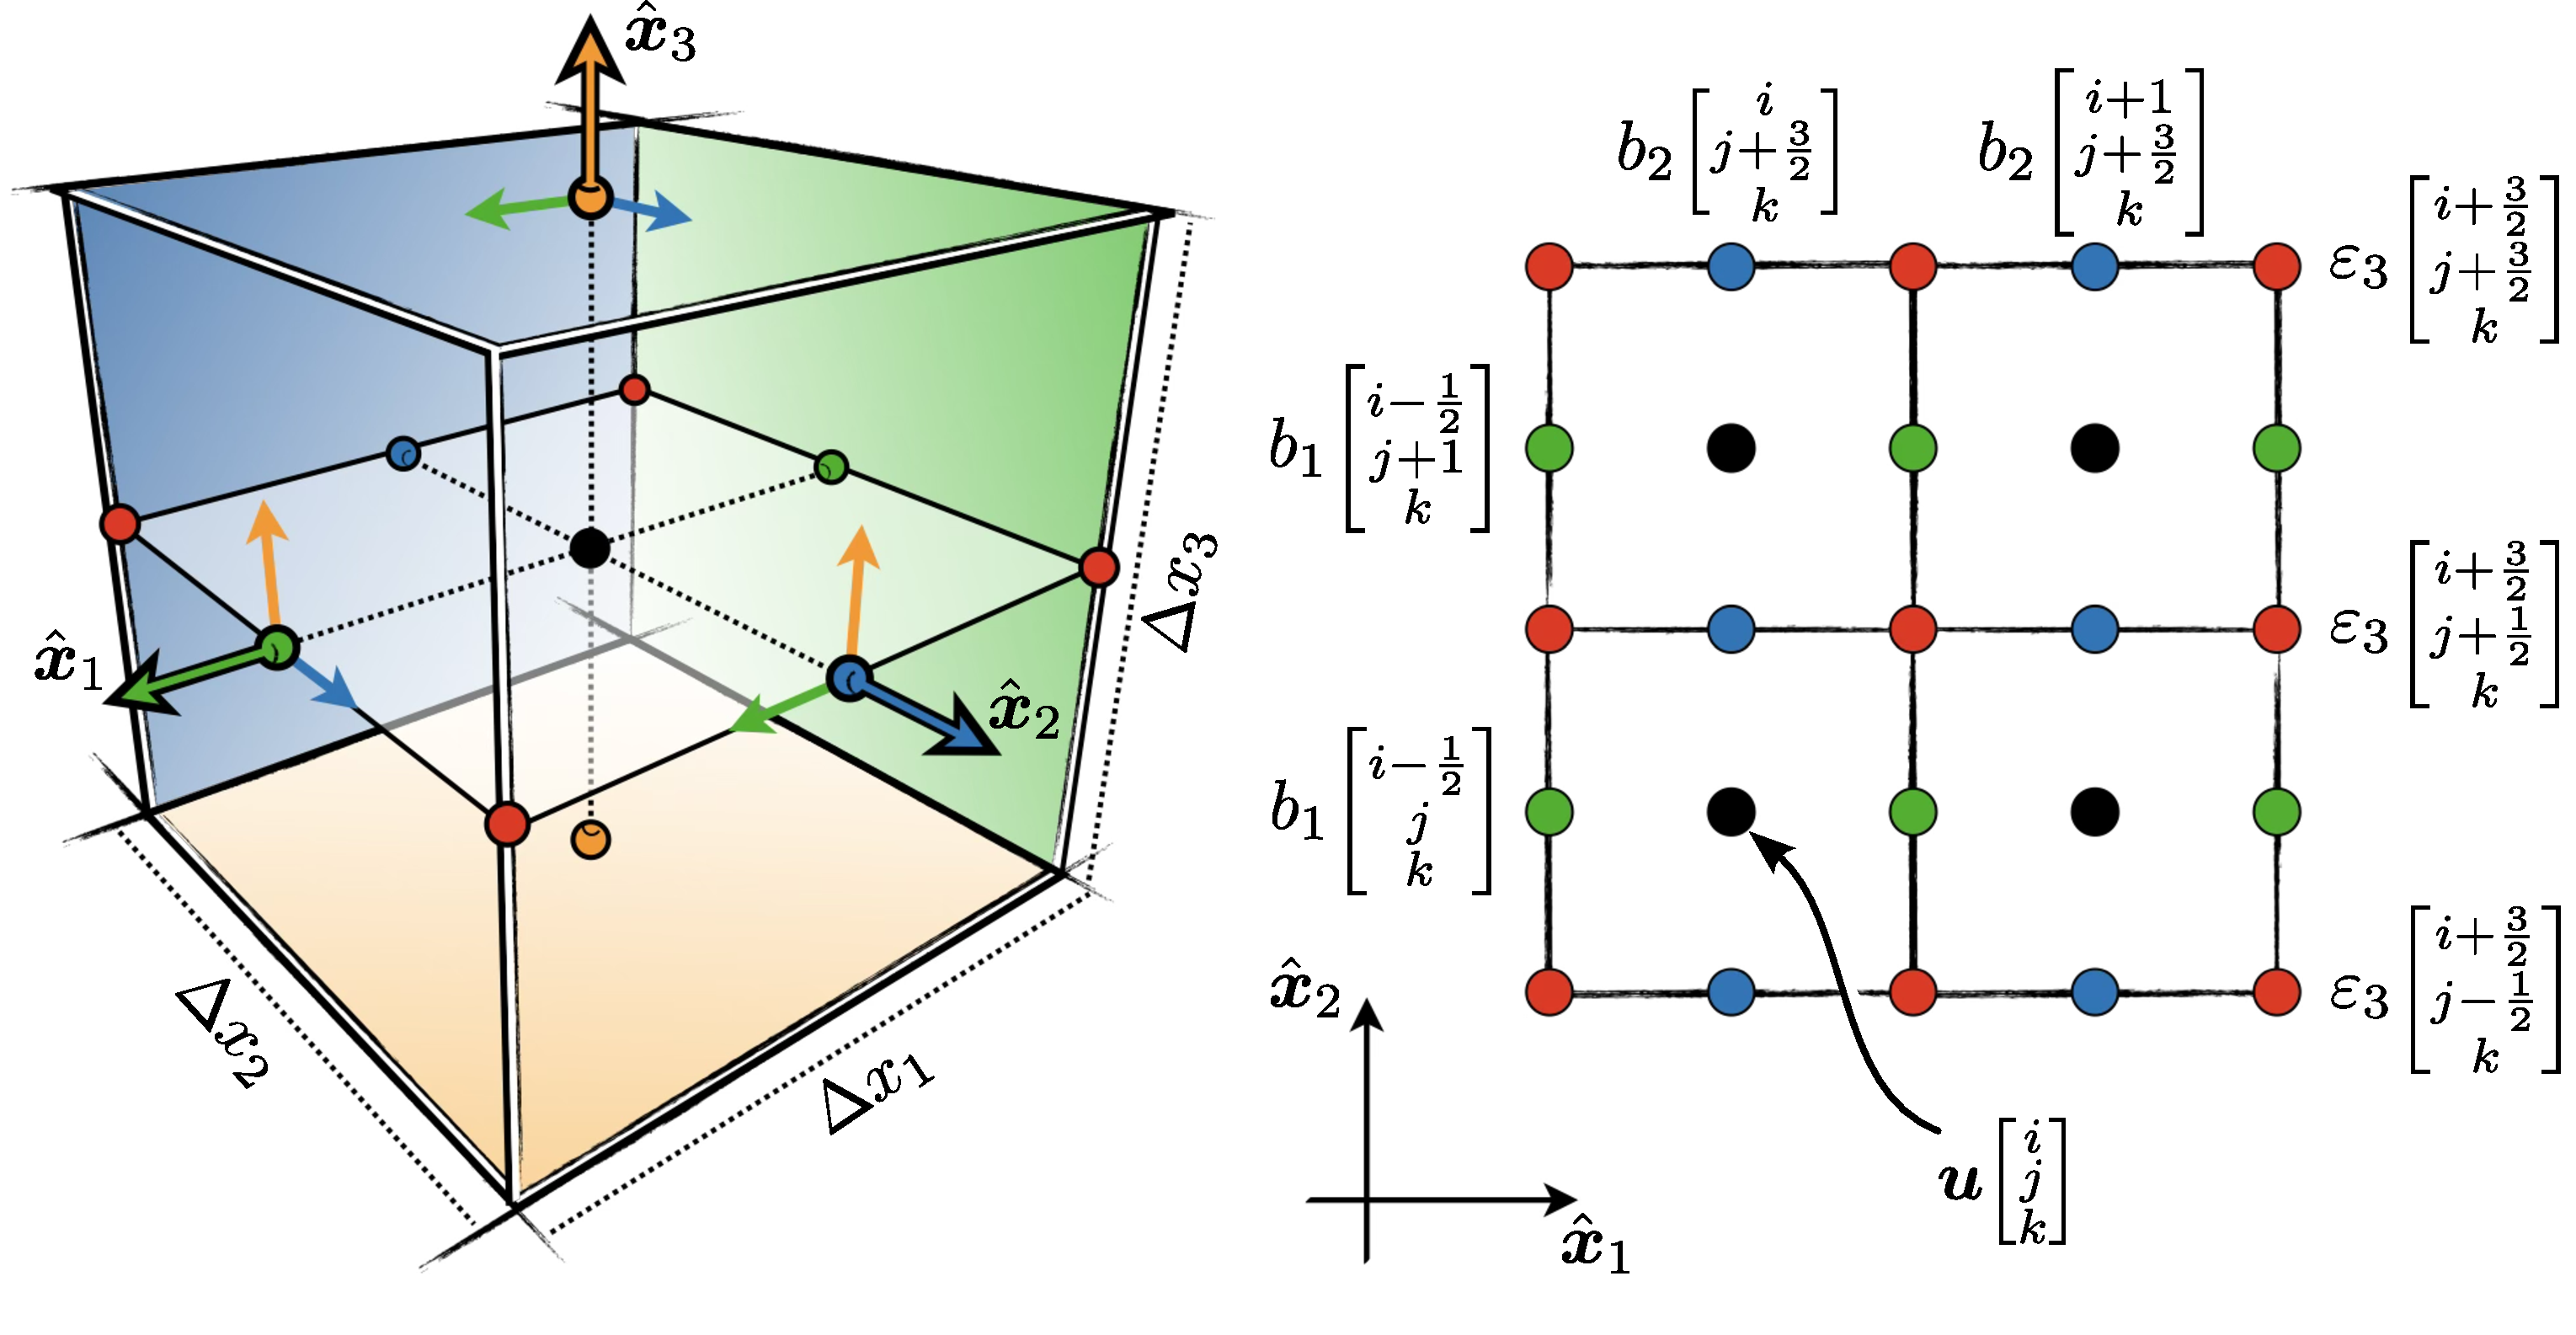
\includegraphics[width=\linewidth]{figures/quokka-mhd/schematics/grid.pdf}
    \caption{The \DIFdelbeginFL \textsc{\DIFdelFL{Quokka}} %DIFAUXCMD
\DIFdelendFL \DIFaddbeginFL \DIFaddFL{\quokka~}\DIFaddendFL mesh shown in perspective view (left) and a slice in the \DIFdelbeginFL \DIFdelFL{$(x_1,x_2)$}\DIFdelendFL \DIFaddbeginFL \DIFaddFL{$(x_0,x_1)$}\DIFaddendFL -plane (right). \DIFdelbeginFL \DIFdelFL{All non-magnetic conserved and primitive variables, for example the fluid velocity $\mVector{u}$, are stored at cell centres }\DIFdelendFL \DIFaddbeginFL \DIFaddFL{Cell-centred quantities }\DIFaddendFL (\DIFdelbeginFL \DIFdelFL{black }\DIFdelendFL \DIFaddbeginFL \DIFaddFL{white }\DIFaddendFL points) \DIFdelbeginFL \DIFdelFL{, denoted by integer indices $ijk$. The three components of the }\DIFdelendFL \DIFaddbeginFL \DIFaddFL{are shown alongside face-centred }\DIFaddendFL magnetic field \DIFdelbeginFL \DIFdelFL{are stored at faces corresponding to their direction }\DIFdelendFL \DIFaddbeginFL \DIFaddFL{components }\DIFaddendFL (blue, \DIFdelbeginFL \DIFdelFL{green}\DIFdelendFL \DIFaddbeginFL \DIFaddFL{yellow}\DIFaddendFL , and \DIFdelbeginFL \DIFdelFL{orange }\DIFdelendFL \DIFaddbeginFL \DIFaddFL{red }\DIFaddendFL points\DIFaddbeginFL \DIFaddFL{, }\DIFaddendFL for the \DIFdelbeginFL \DIFdelFL{faces in the }\DIFdelendFL \DIFaddbeginFL \DIFaddFL{$x_0$, }\DIFaddendFL $x_1$, \DIFdelbeginFL \DIFdelFL{$x_2$, }\DIFdelendFL and \DIFdelbeginFL \DIFdelFL{$x_3$ directions}\DIFdelendFL \DIFaddbeginFL \DIFaddFL{$x_2$ faces respectively}\DIFaddendFL ) \DIFdelbeginFL \DIFdelFL{with one half-integer index }\DIFdelendFL and \DIFdelbeginFL \DIFdelFL{two integer indices; thus for example $b_1$ is stored at $(i - 1/2,j,k)$ and $b_2$ at $(i,j - 1/2,k)$. Finally, the three components of the }\DIFdelendFL \DIFaddbeginFL \DIFaddFL{edge-centred }\DIFaddendFL EMF \DIFdelbeginFL \DIFdelFL{$\mVector{\varepsilon}$ are stored at cell edges }\DIFdelendFL \DIFaddbeginFL \DIFaddFL{components }\DIFaddendFL (\DIFdelbeginFL \DIFdelFL{red }\DIFdelendFL \DIFaddbeginFL \DIFaddFL{green }\DIFaddendFL points)\DIFdelbeginFL \DIFdelFL{with two half-integer indices and one integer index, with the direction of the EMF component parallel to the direction of the cell edge; thus for example $\varepsilon_3$ is stored at $(i - 1/2,j - 1/2,k)$}\DIFdelendFL .}
    \label{fig:schematic:grid}
\DIFdelbeginFL %DIFDELCMD < \end{figure}
%DIFDELCMD < %%%
\DIFdelend \DIFaddbegin \end{figure*}
\DIFaddend

Our implementation uses the staggered mesh scheme first introduced for astrophysical MHD by \citet{Evans88a}, which had precursors in other MHD fields \citep[\eg][]{Yee66a, Brecht81a}; today, this approach is standard in essentially all \DIFdelbegin \DIFdel{three-dimensional }\DIFdelend \DIFaddbegin \DIFadd{3D }\DIFaddend CT schemes \citep[\eg][]{Fromang06a, Gardiner08a, Li12a}. As \DIFdelbegin \DIFdel{illustrate in }%DIFDELCMD < \autoref{fig:schematic:grid}%%%
\DIFdelend \DIFaddbegin \DIFadd{illustrated in \mbox{%DIFAUXCMD
\cref{fig:schematic:grid}}\hskip0pt%DIFAUXCMD
}\DIFaddend , we store all the conserved quantities\DIFaddbegin \DIFadd{, }\DIFaddend except for magnetic fields\DIFaddbegin \DIFadd{, }\DIFaddend at cell centres,\DIFaddbegin \footnote{
    \DIFadd{In addition to the MHD variables described in \mbox{%DIFAUXCMD
\cref{eqn:state:conserved}}\hskip0pt%DIFAUXCMD
, \quokka~also supports a dual-energy formalism, in which the internal energy is evolved alongside the total energy, and (optionally) passive scalars. These quantities extend the conservative state vector, $\mVector{S}_\mathrm{c}$, trivially with extra cell-centred quantities. However, for simplicity in this chapter, we restrict the discussion in this chapter to the minimal set of conserved variables relevant for MHD.
    }\label{fnote:dual-energy}
}
\DIFaddend and thus our vector of conserved cell-centred quantities is
\DIFdelbegin %DIFDELCMD < \begin{align}
%DIFDELCMD <     \mVector{S}_\mathrm{c}\EvalAtH{i}{j}{k}
%DIFDELCMD <         = \begin{Bmatrix}
%DIFDELCMD <             \rho\EvalAtH{i}{j}{k} \\
%DIFDELCMD <             \rho\EvalAtH{i}{j}{k} \mVector{u}\EvalAtH{i}{j}{k} \\
%DIFDELCMD <             e_\mathrm{tot}\EvalAtH{i}{j}{k}
%DIFDELCMD <         \end{Bmatrix}
%DIFDELCMD <     , \label{defn:state-vector}
%DIFDELCMD < \end{align}%%%
\DIFdelend \DIFaddbegin \begin{align}
    \mVector{S}_\mathrm{c}\EvalAtV{i}{j}{k}
        = \begin{Bmatrix}
            \rho\EvalAtH{i}{j}{k} \\
            \rho\EvalAtH{i}{j}{k} \mVector{u}\EvalAtH{i}{j}{k} \\
            e_\mathrm{tot}\EvalAtH{i}{j}{k}
        \end{Bmatrix}
    , \label{eqn:state:conserved}
\end{align}\DIFaddend
where we use integer indices $i$, $j$, and $k$ to denote cell-centred quantities. Each of these quantities should be understood as an average over cell \DIFdelbegin \DIFdel{$(i, j, k)$}\DIFdelend \DIFaddbegin \DIFadd{$\EvalAtH{i}{j}{k}$}\DIFaddend , but for compactness we will omit the angle bracket notation used in \DIFdelbegin %DIFDELCMD < \autoref{eqn:godunov:integral} %%%
\DIFdelend \DIFaddbegin \DIFadd{\mbox{%DIFAUXCMD
\cref{eqn:godunov:integral} }\hskip0pt%DIFAUXCMD
}\DIFaddend from this point forward. \DIFdelbegin \DIFdel{Moreover, for clarity, we define $\mVector{S}_\mathrm{c}$ here for the minimal ideal-MHD system, and note that our dual-energy and passive-scalar extensions correspond with extra cell-centred components (see footnote \ref{fnote:dual-energy}).
 }%DIFDELCMD <

%DIFDELCMD < %%%
\DIFdelend We store the magnetic field on cell faces, with the component normal to a face stored at the face centre (see \DIFdelbegin %DIFDELCMD < \autoref{fig:schematic:grid}%%%
\DIFdelend \DIFaddbegin \DIFadd{\mbox{%DIFAUXCMD
\cref{fig:schematic:grid}}\hskip0pt%DIFAUXCMD
}\DIFaddend ). Thus \DIFdelbegin \DIFdel{$b_1$ }\DIFdelend \DIFaddbegin \DIFadd{$b_0$ }\DIFaddend is indexed as $\,\EvalAtH{i + 1/2}{j}{k}$, \DIFdelbegin \DIFdel{$b_2$ }\DIFdelend \DIFaddbegin \DIFadd{$b_1$ }\DIFaddend as $\,\EvalAtH{i}{j + 1/2}{k}$, and \DIFdelbegin \DIFdel{$b_3$ }\DIFdelend \DIFaddbegin \DIFadd{$b_2$ }\DIFaddend as $\,\EvalAtH{i}{j}{k + 1/2}$. In general, a half-integer index together with two integer indices corresponds with a face-centred quantity that has been face-averaged. We also use edge-centred quantities\DIFdelbegin \DIFdel{which is }\DIFdelend \DIFaddbegin \DIFadd{, which are }\DIFaddend associated with two half-integer indices, for example $\EvalAtH{i + 1/2}{j + 1/2}{k}$, which indicates an edge-averaged \DIFdelbegin \DIFdel{values}\DIFdelend \DIFaddbegin \DIFadd{value stored on the $x_2$-edge}\DIFaddend .

%DIF <  Our implementation also supports the use of a dual energy formalism, in which we treat the internal energy as a quantity distinct from the total energy, and the use of passive scalars to represent mass fractions of different species. Either of these options adds additional conserved quantities to the state vector $\mVector{S}_\mathrm{c}$. For simplicity, however, we will limit our discussion here to the case where the only conserved quantities are the five listed in \autoref{defn:state-vector}. Extension to additional conserved quantities is no different for MHD than it is for hydrodynamics.
\DIFdelbegin %DIFDELCMD <

%DIFDELCMD < %%%
\DIFdelend \subsection{Flux calculation}
\label{sec:methods:flux}

As discussed in \DIFdelbegin %DIFDELCMD < \autoref{sec:intro:goals}%%%
\DIFdelend \DIFaddbegin \DIFadd{\sref{sec:intro:goals}}\DIFaddend , the first \DIFdelbegin \DIFdel{required }\DIFdelend step for a Godunov scheme \DIFdelbegin \DIFdel{for ideal MHD }\DIFdelend is a recipe to compute the fluxes of the cell-averaged quantities across cell faces. This step in turn has two parts: \DIFdelbegin \DIFdel{an interpolation }\DIFdelend \DIFaddbegin \DIFadd{a reconstruction }\DIFaddend scheme used to \DIFdelbegin \DIFdel{compute interface }\DIFdelend \DIFaddbegin \DIFadd{reconstruct primitive }\DIFaddend states on either side of \DIFdelbegin \DIFdel{the face, and }\DIFdelend \DIFaddbegin \DIFadd{cell interfaces, and then }\DIFaddend a Riemann solver to compute \DIFdelbegin \DIFdel{fluxes from those interfacestates}\DIFdelend \DIFaddbegin \DIFadd{the resulting flux through the interface}\DIFaddend .

\DIFdelbegin \DIFdel{For the interpolation part of the scheme, our approach }\DIFdelend \DIFaddbegin \DIFadd{The reconstruction part of our scheme }\DIFaddend closely follows the \DIFdelbegin \DIFdel{one }\textsc{\DIFdel{Quokka}} %DIFAUXCMD
\DIFdelend \DIFaddbegin \DIFadd{approach \quokka~already }\DIFaddend uses for pure hydrodynamics, as described in \citetalias{Wibking22a}. \DIFdelbegin \DIFdel{Thus here we only summarise and identify points of difference necessitated }\DIFdelend \DIFaddbegin \DIFadd{We therefore only summarise it here, and highlight the differences introduced }\DIFaddend by the inclusion of magnetic fields. We first convert our vector of conserved variables to a vector of cell-centred primitive variables that includes the magnetic field:
\DIFdelbegin %DIFDELCMD < \begin{align}
%DIFDELCMD <     \mVector{S}_\mathrm{p}\EvalAtH{i}{j}{k}
%DIFDELCMD <         = \begin{Bmatrix}
%DIFDELCMD <             \rho\EvalAtH{i}{j}{k} \\
%DIFDELCMD <             \mVector{u}\EvalAtH{i}{j}{k} \\
%DIFDELCMD <             p\EvalAtH{i}{j}{k} \\
%DIFDELCMD <             \mVector{b}\EvalAtH{i}{j}{k}
%DIFDELCMD <         \end{Bmatrix}
%DIFDELCMD <     ,
%DIFDELCMD < \end{align}%%%
\DIFdelend \DIFaddbegin \begin{align}
    \mVector{S}_\mathrm{p}\EvalAtV{i}{j}{k}
        = \begin{Bmatrix}
            \rho\EvalAtH{i}{j}{k} \\
            \mVector{u}\EvalAtH{i}{j}{k} \\
            p\EvalAtH{i}{j}{k} \\
            \mVector{b}\EvalAtH{i}{j}{k}
        \end{Bmatrix}
    , \label{eqn:state:primitive}
\end{align}\DIFaddend
where $p$ is the gas pressure. We compute the magnetic field in this step by \DIFdelbegin \DIFdel{simple averaging of }\DIFdelend \DIFaddbegin \DIFadd{simply averaging }\DIFaddend the adjacent face-centred data, \ie we take
\DIFdelbegin %DIFDELCMD < \begin{align}
%DIFDELCMD <     b_1\EvalAtH{i}{j}{k}
%DIFDELCMD <         = \frac{1}{2} \rbrac{
%DIFDELCMD <             b_1\EvalAtH{i + 1/2}{j}{k} + b_1\EvalAtH{i - 1/2}{j}{k}
%DIFDELCMD <         }
%DIFDELCMD < \end{align}%%%
\DIFdelend \DIFaddbegin \begin{align}
    b_0\EvalAtV{i}{j}{k}
        = \frac{1}{2} \rbrac{
            b_0\EvalAtV{i + 1/2}{j}{k} + b_0\EvalAtV{i - 1/2}{j}{k}
        }
\end{align}\DIFaddend
and similarly for \DIFdelbegin \DIFdel{$b_2\EvalAtH{i}{j}{k}$ and $b_3\EvalAtH{i}{j}{k}$}\DIFdelend \DIFaddbegin \DIFadd{$b_1\EvalAtH{i}{j}{k}$ and $b_2\EvalAtH{i}{j}{k}$}\DIFaddend .

Next\DIFaddbegin \DIFadd{, }\DIFaddend we reconstruct $\mVector{S}_\mathrm{p}$ \DIFaddbegin \DIFadd{at faces }\DIFaddend from cell centres \DIFdelbegin \DIFdel{to faces in order to obtain the left and right states at each interface, We compute the interface states using one-dimensional }\DIFdelend \DIFaddbegin \DIFadd{using 1D }\DIFaddend polynomial reconstruction along each coordinate direction\DIFdelbegin \DIFdel{. }\textsc{\DIFdel{Quokka}} %DIFAUXCMD
\DIFdelend \DIFaddbegin \DIFadd{, obtaining left and right states at each interface. \quokka~}\DIFaddend supports piecewise-constant reconstruction (\ie we take the primitive state vector at the face of each cell to be equal to the cell-centred primitive state), a piecewise linear method (PLM) using either a monotonized-central or minmod slope limiter \citep{van-Leer74a}, a piecewise parabolic method (PPM) similar to that of \citet{Colella84a} but with a modified approach to monotonicity preservation (see \citetalias{Wibking22a} for details), and the extremum-preserving PPM method (PPM-EP) described by \citet{Rider07a}. We will test several of these choices in \DIFdelbegin %DIFDELCMD < \autoref{sec:performance}%%%
\DIFdelend \DIFaddbegin \DIFadd{\sref{sec:scheme-comparisons}}\DIFaddend . Note that, for the magnetic fields\DIFaddbegin \DIFadd{, }\DIFaddend we reconstruct only the components transverse to the reconstruction direction, since \DIFdelbegin \DIFdel{we }\DIFdelend the normal component is already available at the face. \DIFdelbegin \DIFdel{Thus for example}\DIFdelend \DIFaddbegin \DIFadd{For example, }\DIFaddend if we are reconstructing in the \DIFdelbegin \DIFdel{$x_1$ }\DIFdelend \DIFaddbegin \DIFadd{$x_0$ }\DIFaddend direction, we reconstruct only \DIFdelbegin \DIFdel{$b_2$ and $b_3$ to }\DIFdelend \DIFaddbegin \DIFadd{$b_1$ and $b_2$ at }\DIFaddend the face, and \DIFdelbegin \DIFdel{we directly }\DIFdelend use the value of \DIFdelbegin \DIFdel{$b_1$ stored at the face}\DIFdelend \DIFaddbegin \DIFadd{$b_0$ already stored there directly}\DIFaddend .

The final step of the flux calculation is \DIFdelbegin \DIFdel{solution of }\DIFdelend \DIFaddbegin \DIFadd{to solve }\DIFaddend the Riemann problem. Our default method for this is the HLLD Riemann solver \citep{Miyoshi05a}. HLLD returns (i) the face-centred fluxes $\mVector{F}$ that enter the finite-volume updates of $\rho$, $\rho\mVector{u}$, and $e_\mathrm{tot}$, and (ii) a set of resolved interface states, including the normal and transverse components of $\mVector{u}$ and $\mVector{b}$ associated with the intermediate waves in the Riemann fan. In our CT formulation we do not use the magnetic part of the HLLD flux to advance $\mVector{b}$; instead, we use the upwinded interface states when constructing edge-centred EMFs for the magnetic update, as described in \DIFdelbegin %DIFDELCMD < \autoref{sec:methods:emf}%%%
\DIFdelend \DIFaddbegin \DIFadd{\sref{sec:methods:emf}}\DIFaddend . We therefore store these interface states for use in the next step.

To improve robustness in challenging flows\DIFaddbegin \DIFadd{, }\DIFaddend we also apply two local stabilisation corrections at the level of the numerical fluxes in the HLLD solver. The first is a carbuncle fix for grid-aligned strong shocks, based on a pressure-sensitive blending of transverse dissipation. The second is a low-Mach pressure rescaling that restores the correct \DIFdelbegin \DIFdel{$\mathcal{O}(\mathcal{M}^2)$ }\DIFdelend \DIFaddbegin \DIFadd{$\bigO{\mathcal{M}^2}$ }\DIFaddend scaling of pressure perturbations in the limit $\mathcal{M} \rightarrow 0$. For both these fixes we follow the method of \citet{Minoshima21a}.

\DIFdelbegin \DIFdel{Finally, in }\DIFdelend \DIFaddbegin \DIFadd{In }\DIFaddend addition to the HLLD Riemann solver, we also implement a Local Lax-Friedrichs (LLF) solver \citep{Rusanov62a}\DIFdelbegin \DIFdel{. This }\DIFdelend \DIFaddbegin \DIFadd{, which }\DIFaddend returns the same quantities \DIFdelbegin \DIFdel{as the HLLD solver, }\DIFdelend but is much more dissipative. We \DIFdelbegin \DIFdel{will make use of }\DIFdelend \DIFaddbegin \DIFadd{use }\DIFaddend this more dissipative flux in our flux correction \DIFdelbegin \DIFdel{scheme, which we describe in full below in }%DIFDELCMD < \autoref{sec:methods:time-stepping}%%%
\DIFdelend \DIFaddbegin \DIFadd{strategy, described in full in \sref{sec:methods:time-stepping}}\DIFaddend .

\subsection{EMF calculation}
\label{sec:methods:emf}

The second step in advancing the MHD equations in time, which occurs after the flux calculation described in the previous section, is calculation of the EMFs required to update the magnetic field. As with the flux calculation, this involves two steps: first reconstructing either the EMFs or the quantities required to compute them \DIFdelbegin \DIFdel{to }\DIFdelend \DIFaddbegin \DIFadd{at }\DIFaddend the cell edges where the EMFs are needed, and then combining the results of this reconstruction into a single EMF that can be used to update the magnetic field. In what follows, we will for notational simplicity specialise to the case of an update in the \DIFdelbegin \DIFdel{$x_1$ }\DIFdelend \DIFaddbegin \DIFadd{$x_0$ }\DIFaddend direction, for which the face has edges oriented in the \DIFdelbegin \DIFdel{$x_2$}\DIFdelend \DIFaddbegin \DIFadd{$x_1$}\DIFaddend - and \DIFdelbegin \DIFdel{$x_3$-direction}\DIFdelend \DIFaddbegin \DIFadd{$x_2$-directions}\DIFaddend ; the corresponding procedures for other directions can be obtained by cyclic permutation of the indices. Thus our goal for cell \DIFdelbegin \DIFdel{$(i, j, k)$ }\DIFdelend \DIFaddbegin \DIFadd{$\EvalAtH{i}{j}{k}$ }\DIFaddend is to arrive at estimates for the four average EMFs on the edges surrounding face \DIFdelbegin \DIFdel{$(i + 1/2, j, k)$}\DIFdelend \DIFaddbegin \DIFadd{$\EvalAtH{i + 1/2}{j}{k}$}\DIFaddend , so that we can write the semi-discrete evolution equation (\DIFdelbegin %DIFDELCMD < \autoref{eqn:ct_stokes_intro}%%%
\DIFdel{) as
}%DIFDELCMD < \begin{align}
%DIFDELCMD <     &\mppFrac{b_1}{t}\EvalAtH{i + 1/2}{j}{k}
%DIFDELCMD <         =  \frac{-1}{\Delta{x_2}\, \Delta{x_3}} \Bigg(
%DIFDELCMD <             \Delta{x_2} \, \varepsilon_2\EvalAtH{i + 1/2}{j - 1/2}{k}
%DIFDELCMD <         \nonumber \\
%DIFDELCMD <         &\nquad[3]
%DIFDELCMD <             + \Delta{x_3} \, \varepsilon_3\EvalAtH{i + 1/2}{j}{k - 1/2}
%DIFDELCMD <             - \Delta{x_2} \, \varepsilon_2 \EvalAtH{i + 1/2}{j + 1/2}{k}
%DIFDELCMD <         \nonumber \\
%DIFDELCMD <         &\nquad[5]
%DIFDELCMD <             - \Delta{x_3} \, \varepsilon_3\EvalAtH{i + 1/2}{j}{k + 1/2}
%DIFDELCMD <         \Bigg)
%DIFDELCMD <     , \label{eqn:dbdt:discrete}
%DIFDELCMD < \end{align}%%%
\DIFdelend \DIFaddbegin \DIFadd{\mbox{%DIFAUXCMD
\cref{eqn:ct:circulation-update}}\hskip0pt%DIFAUXCMD
) as
}\begin{align}
    \mpFrac{b_0}{t}\EvalAtV{i + 1/2}{j}{k}
        &=  \frac{1}{\Delta{x_1}\, \Delta{x_2}} \Bigg(
            \Delta{x_2} \, \varepsilon_2\EvalAtV{i + 1/2}{j - 1/2}{k}
            + \Delta{x_1} \, \varepsilon_1\EvalAtV{i + 1/2}{j}{k + 1/2}
        \nonumber \\
        &\nquad[5]
            - \Delta{x_2} \, \varepsilon_2\EvalAtV{i + 1/2}{j + 1/2}{k}
            - \Delta{x_1} \, \varepsilon_1\EvalAtV{i + 1/2}{j}{k - 1/2}
        \Bigg)
    , \label{eqn:dbdt:discrete}
\end{align}\DIFaddend
where \DIFdelbegin \DIFdel{$\Delta{x_2}$ and $\Delta{x_3}$ }\DIFdelend \DIFaddbegin \DIFadd{$\Delta{x_1}$ and $\Delta{x_2}$ }\DIFaddend are the cell widths in the \DIFdelbegin \DIFdel{$x_2$}\DIFdelend \DIFaddbegin \DIFadd{$x_1$}\DIFaddend - and \DIFdelbegin \DIFdel{$x_3$}\DIFdelend \DIFaddbegin \DIFadd{$x_2$}\DIFaddend -directions.

\subsubsection{The \DIFdelbegin \DIFdel{reconstruction }\DIFdelend \DIFaddbegin \DIFadd{EMF compute }\DIFaddend scheme}
\DIFdelbegin %DIFDELCMD < \label{sec:methods:emf:reconstruction}
%DIFDELCMD < %%%
\DIFdelend \DIFaddbegin \label{sec:methods:emf:compute}
\DIFaddend

In \DIFdelbegin \DIFdel{explaining our reconstruction method, we will further specialise to explaining the procedure to reconstruct the EMFs }\DIFdelend \DIFaddbegin \DIFadd{the following we will explain the procedure for computing the EMF component }\DIFaddend only on the \DIFdelbegin \DIFdel{$x_3$}\DIFdelend \DIFaddbegin \DIFadd{$x_2$}\DIFaddend -edge, \DIFdelbegin \DIFdel{$\varepsilon_3\EvalAtH{i + 1/2}{j \pm 1/2}{k}$}\DIFdelend \DIFaddbegin \DIFadd{$\varepsilon_2\EvalAtH{i + 1/2}{j \pm 1/2}{k}$}\DIFaddend , since one can then \DIFdelbegin \DIFdel{generate the corresponding procedure to }\DIFdelend compute the EMFs on \DIFdelbegin \DIFdel{other edges by }\DIFdelend \DIFaddbegin \DIFadd{the other edges through }\DIFaddend cyclic index permutation. We \DIFaddbegin \DIFadd{will }\DIFaddend consider three schemes\DIFdelbegin \DIFdel{to reconstruct this quantity: two that have previously appeared }\DIFdelend \DIFaddbegin \DIFadd{: two implemented as published }\DIFaddend in the literature, and \DIFdelbegin \DIFdel{one new one that we introduce}\DIFdelend \DIFaddbegin \DIFadd{a third that is a modified version of an existing approach}\DIFaddend .

\begin{figure}
    \centering
    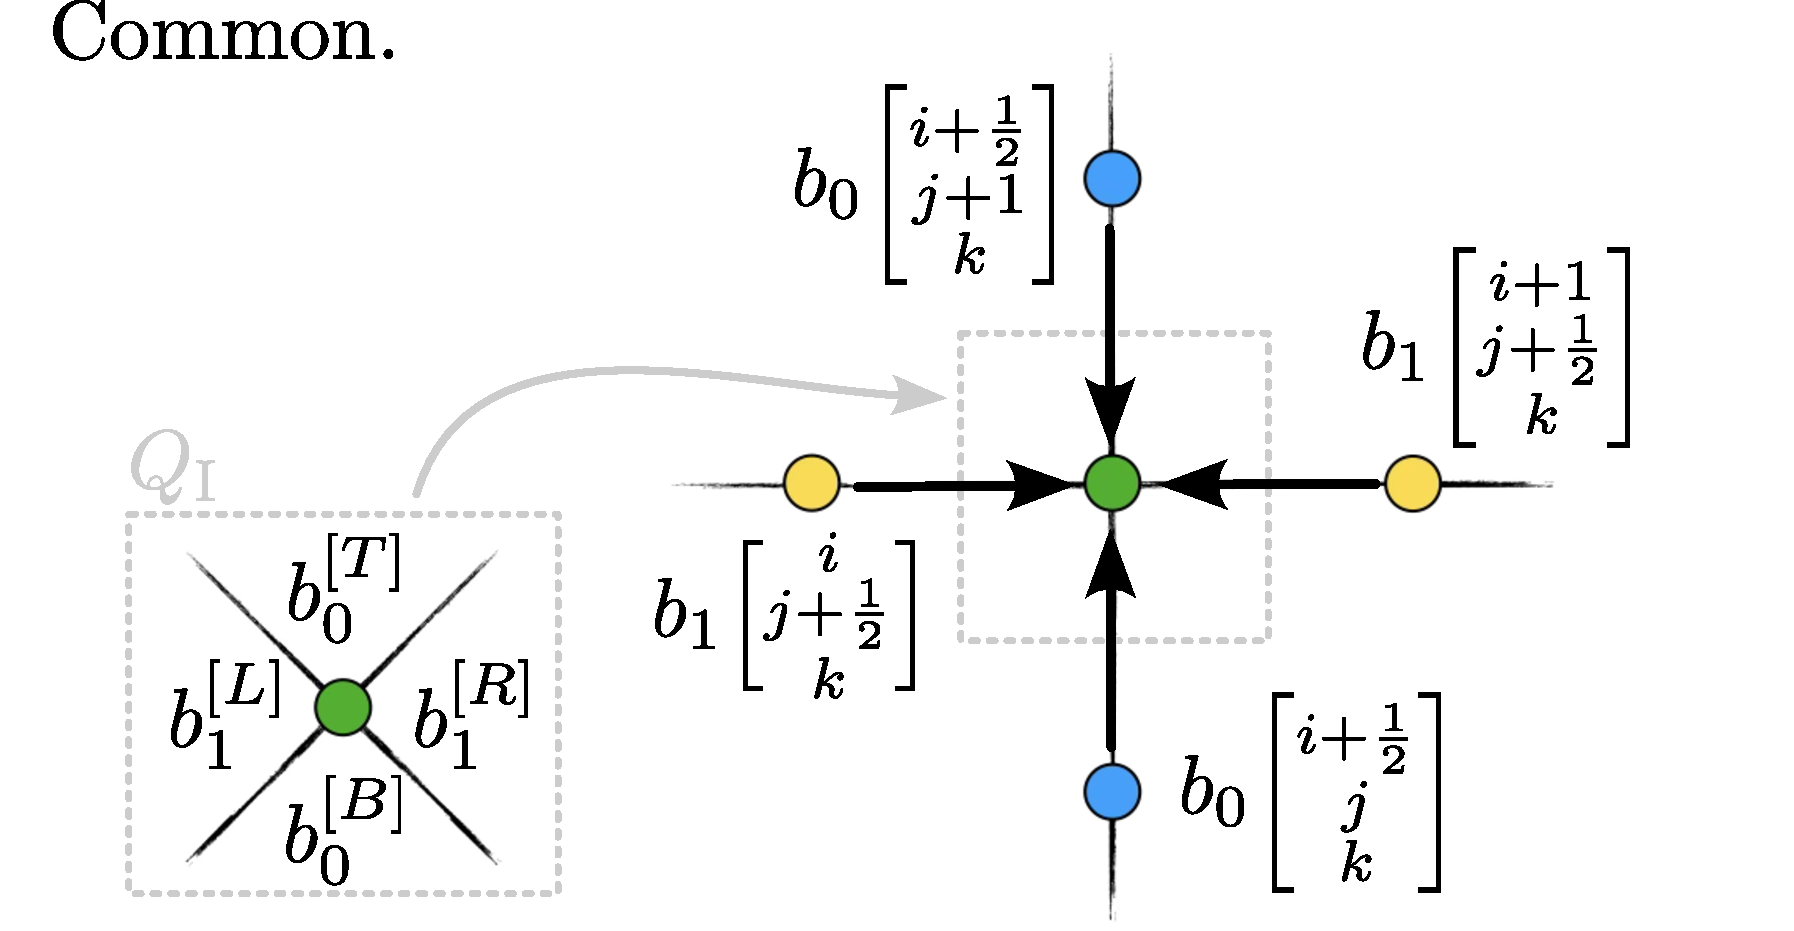
\includegraphics[width=0.65\linewidth]{figures/quokka-mhd/schematics/b-common.pdf}
    \caption{\DIFdelbeginFL \DIFdelFL{Schematic representation }\DIFdelendFL \DIFaddbeginFL \DIFaddFL{Reconstruction }\DIFaddendFL of \DIFdelbeginFL \DIFdelFL{the magnetic field reconstruction step, which is common to all our EMF reconstruction schemes. In this step, }\DIFdelendFL face-centred magnetic fields \DIFdelbeginFL \DIFdelFL{are interpolated }\DIFdelendFL to \DIFdelbeginFL \DIFdelFL{cell corners. In }\DIFdelendFL the \DIFdelbeginFL \DIFdelFL{example shown above, the face-centred magnetic field component $b_1$, stored at the $x_1$ }\DIFdelendFL cell \DIFdelbeginFL \DIFdelFL{faces }\DIFdelendFL \DIFaddbeginFL \DIFaddFL{edge }\DIFaddendFL (\DIFdelbeginFL \DIFdelFL{blue points}\DIFdelendFL \DIFaddbeginFL \DIFaddFL{green point}\DIFaddendFL ), \DIFdelbeginFL \DIFdelFL{is interpolated }\DIFdelendFL \DIFaddbeginFL \DIFaddFL{common }\DIFaddendFL to \DIFdelbeginFL \DIFdelFL{the cell edge }\DIFdelendFL \DIFaddbeginFL \DIFaddFL{all EMF compute schemes: $b_0$ }\DIFaddendFL (\DIFdelbeginFL \DIFdelFL{red point)}\DIFdelendFL \DIFaddbeginFL \DIFaddFL{blue points}\DIFaddendFL , \DIFdelbeginFL \DIFdelFL{yielding magnetic field components $b_1^{\{B\}}$ and $b_1^{\{T\}}$ at the bottom and top of the edge. Similarly, component $b_2$, stored at $x_2$ cell }\DIFdelendFL \DIFaddbeginFL \DIFaddFL{$x_0$ }\DIFaddendFL faces\DIFaddbeginFL \DIFaddFL{) yields $b_0^{[B]}$ and $b_0^{[T]}$; $b_1$ }\DIFaddendFL (\DIFdelbeginFL \DIFdelFL{green }\DIFdelendFL \DIFaddbeginFL \DIFaddFL{yellow }\DIFaddendFL points\DIFdelbeginFL \DIFdelFL{)}\DIFdelendFL , \DIFdelbeginFL \DIFdelFL{is interpolated to the cell edge to yield $b_2^{\{L\}}$ }\DIFdelendFL \DIFaddbeginFL \DIFaddFL{$x_1$ faces) yields $b_1^{[L]}$ }\DIFaddendFL and \DIFdelbeginFL \DIFdelFL{$b_2^{\{R\}}$, values on the left and right side of the edge}\DIFdelendFL \DIFaddbeginFL \DIFaddFL{$b_1^{[R]}$}\DIFaddendFL .}
    \label{fig:schematic:b-common}
\end{figure}

All of the schemes start in the same way, which we illustrate in \DIFdelbegin %DIFDELCMD < \autoref{fig:schematic:b-common}%%%
\DIFdelend \DIFaddbegin \DIFadd{\mbox{%DIFAUXCMD
\cref{fig:schematic:b-common}}\hskip0pt%DIFAUXCMD
}\DIFaddend . We first reconstruct the face-centred magnetic field component \DIFdelbegin \DIFdel{$b_1\EvalAtH{i \pm 1/2}{j}{k}$ in the $x_2$}\DIFdelend \DIFaddbegin \DIFadd{$b_0\EvalAtH{i \pm 1/2}{j}{k}$ in the $x_1$}\DIFaddend - direction to yield \DIFdelbegin \DIFdel{$b_{1}^{\cbrac{S_\mathrm{II}}}\EvalAtH{i \pm 1/2}{j \pm 1/2}{k}$}\DIFdelend \DIFaddbegin \DIFadd{$b_{0}^{[S_\mathrm{II}]}\EvalAtH{i \pm 1/2}{j \pm 1/2}{k}$}\DIFaddend , and reconstruct the face-centred magnetic field component \DIFdelbegin \DIFdel{$b_2\EvalAtH{i}{j \pm 1/2}{k}$ in the $x_1$}\DIFdelend \DIFaddbegin \DIFadd{$b_1\EvalAtH{i}{j \pm 1/2}{k}$ in the $x_0$}\DIFaddend -direction to yield \DIFdelbegin \DIFdel{$b_{2}^{\cbrac{S_\mathrm{I}}}\EvalAtH{i \pm 1/2}{j \pm 1/2}{k}$}\DIFdelend \DIFaddbegin \DIFadd{$b_{1}^{[S_\mathrm{I}]}\EvalAtH{i \pm 1/2}{j \pm 1/2}{k}$}\DIFaddend . Here the subscripts \DIFdelbegin \DIFdel{$L$ or $R$ }\DIFdelend \DIFaddbegin \DIFadd{$S_\mathrm{I} \in \{L, R\}$ }\DIFaddend indicate values on the left and right side of an \DIFdelbegin \DIFdel{$x_1$}\DIFdelend \DIFaddbegin \DIFadd{$x_0$}\DIFaddend -face, and similarly \DIFdelbegin \DIFdel{the subscripts $B$ and $T$ }\DIFdelend \DIFaddbegin \DIFadd{$S_\mathrm{II} \in \{B, T\}$ }\DIFaddend indicate the values on the bottom and top of \DIFdelbegin \DIFdel{a $x_2$}\DIFdelend \DIFaddbegin \DIFadd{an $x_1$}\DIFaddend -face.\footnote{
    Formally there is of course no difference between ``left'' and ``bottom'', or between ``right'' and ``top'', but we use different terminology to help make clear whether we are discussing an interface oriented in the \DIFdelbegin \DIFdel{$x_1$}\DIFdelend \DIFaddbegin \DIFadd{$x_0$}\DIFaddend -direction, which uses left and right, and one in the \DIFdelbegin \DIFdel{$x_2$}\DIFdelend \DIFaddbegin \DIFadd{$x_1$}\DIFaddend -direction, which uses top and bottom.
} The $L$ and $R$ values, and the $B$ and $T$ values, may be different due to limiting in the reconstruction. This reconstruction, and all the other reconstruction steps we will describe below, can be done using any of the PC, PLM, PPM, or PPM-EP \DIFdelbegin \DIFdel{interpolators described in }%DIFDELCMD < \autoref{sec:methods:flux} %%%
\DIFdel{-- }\DIFdelend \DIFaddbegin \DIFadd{reconstruction methods described in \sref{sec:methods:flux}; }\DIFaddend the choices of \DIFdelbegin \DIFdel{reconstruction scheme and interpolator }\DIFdelend \DIFaddbegin \DIFadd{EMF compute scheme and reconstruction method }\DIFaddend are independent. Below in \DIFdelbegin %DIFDELCMD < \autoref{sec:performance} %%%
\DIFdelend \DIFaddbegin \DIFadd{\sref{sec:scheme-comparisons} }\DIFaddend we will test multiple combinations of \DIFdelbegin \DIFdel{interpolator and reconstruction scheme}\DIFdelend \DIFaddbegin \DIFadd{EMF compute scheme and reconstruction method}\DIFaddend .

Once the magnetic fields are reconstructed \DIFdelbegin \DIFdel{to }\DIFdelend \DIFaddbegin \DIFadd{at }\DIFaddend the cell edges, the remaining steps differ depending on the scheme.

\begin{figure}
    \centering
    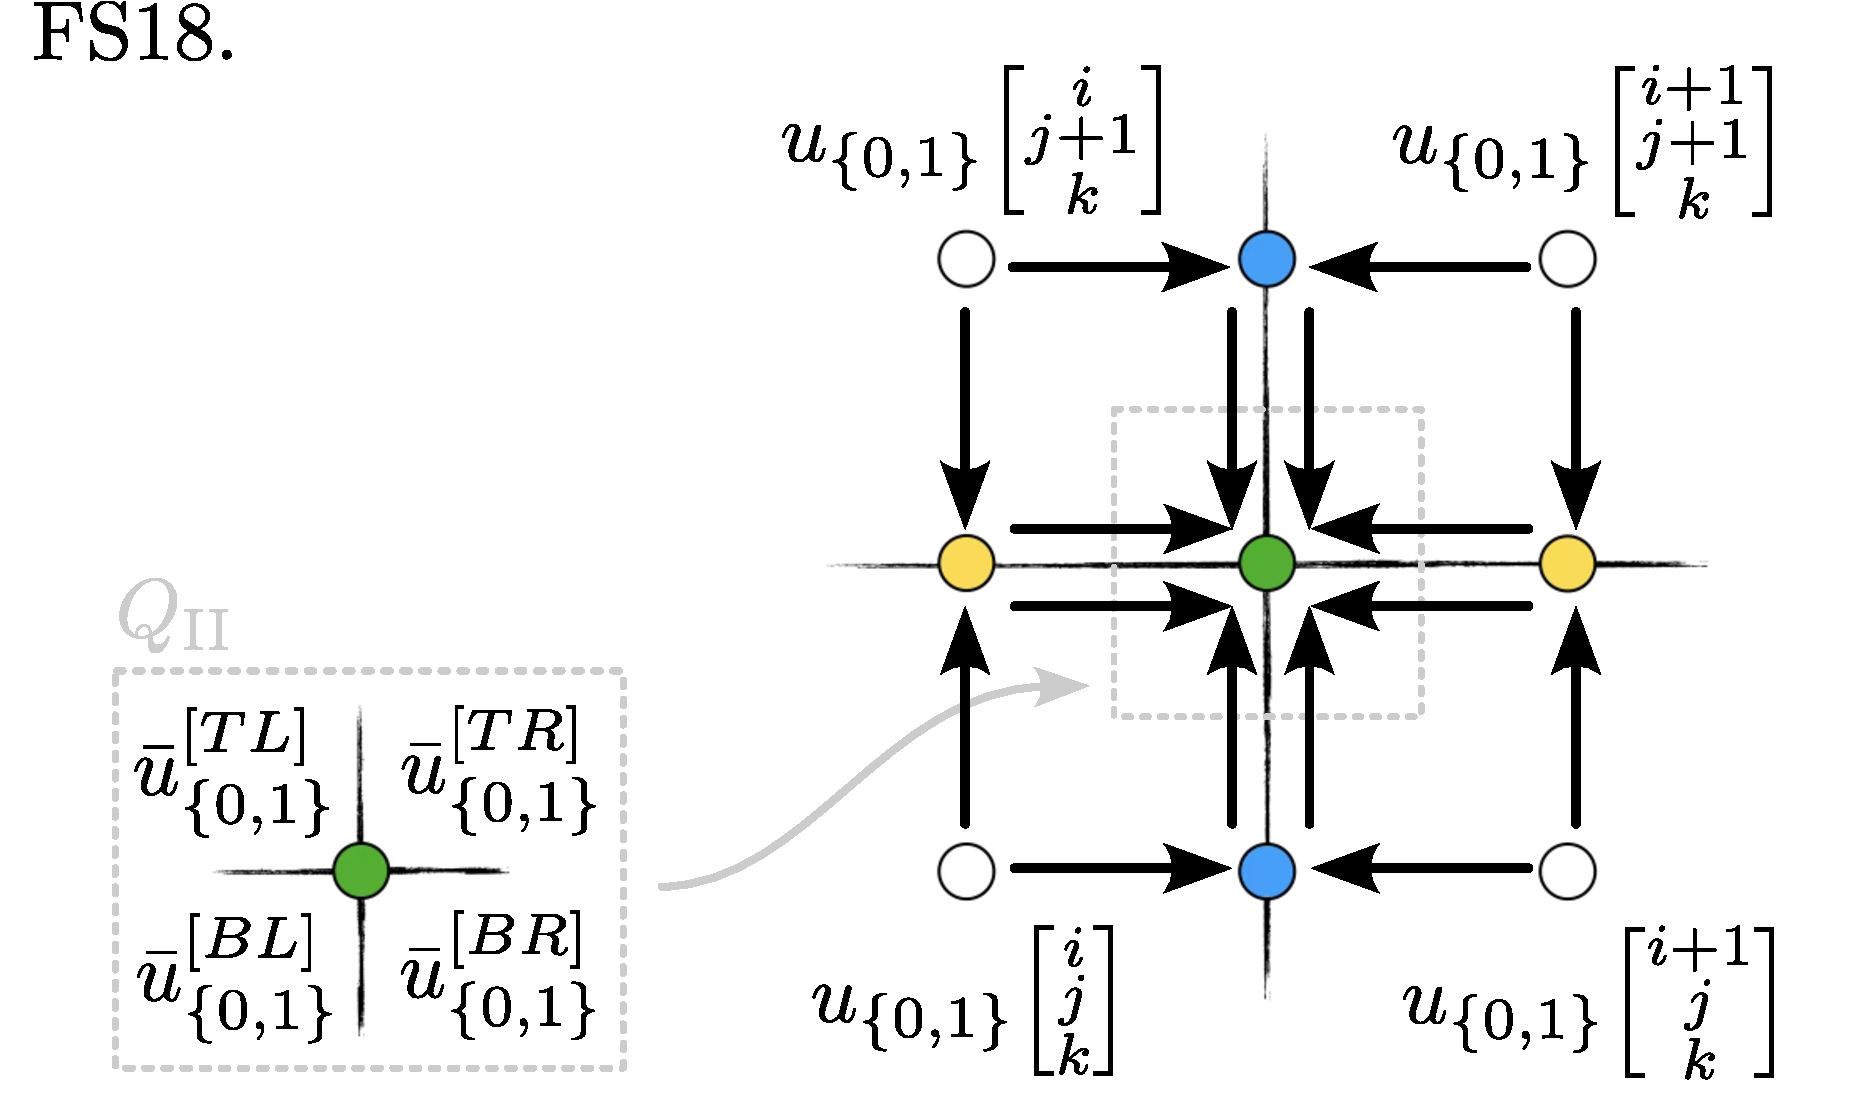
\includegraphics[width=0.65\linewidth]{figures/quokka-mhd/schematics/u-fs18.pdf}
    \caption{\DIFdelbeginFL \DIFdelFL{Schematic representation of }\DIFdelendFL \DIFaddbeginFL \DIFaddFL{Velocity reconstruction for }\DIFaddendFL the \DIFdelbeginFL \DIFdelFL{velocity interpolation part of the }\DIFdelendFL \citetalias{Felker18a} \DIFdelbeginFL \DIFdelFL{EMF reconstruction }\DIFdelendFL \DIFaddbeginFL \DIFaddFL{compute }\DIFaddendFL scheme\DIFdelbeginFL \DIFdelFL{. In this scheme, the velocity components $u_1$ }\DIFdelendFL \DIFaddbeginFL \DIFaddFL{: cell-centred $u_0$ }\DIFaddendFL and \DIFdelbeginFL \DIFdelFL{$u_2$ stored at cell centres }\DIFdelendFL \DIFaddbeginFL \DIFaddFL{$u_1$ }\DIFaddendFL (\DIFdelbeginFL \DIFdelFL{black points}\DIFdelendFL \DIFaddbeginFL \DIFaddFL{white point}\DIFaddendFL ) are \DIFdelbeginFL \DIFdelFL{interpolated }\DIFdelendFL \DIFaddbeginFL \DIFaddFL{reconstructed }\DIFaddendFL to \DIFdelbeginFL \DIFdelFL{the edge (red point) in two steps -- first by interpolating to the }\DIFdelendFL cell faces \DIFdelbeginFL \DIFdelFL{in the $x_1$ and $x_2$ directions }\DIFdelendFL (blue and \DIFdelbeginFL \DIFdelFL{green }\DIFdelendFL \DIFaddbeginFL \DIFaddFL{yellow }\DIFaddendFL points) \DIFdelbeginFL \DIFdelFL{, then by interpolating in the $x_2$ }\DIFdelendFL and \DIFdelbeginFL \DIFdelFL{$x_1$ directions }\DIFdelendFL \DIFaddbeginFL \DIFaddFL{then }\DIFaddendFL to \DIFdelbeginFL \DIFdelFL{reach }\DIFdelendFL the cell edge \DIFaddbeginFL \DIFaddFL{(green point)}\DIFaddendFL , yielding \DIFdelbeginFL \DIFdelFL{two estimates of the velocity at the edge. The two estimates are then averaged to yield $\bar{u}_{1,2}$. This process occurs in each of the }\DIFdelendFL four \DIFdelbeginFL \DIFdelFL{corners adjacent to the edge, yielding four values $\bar{u}_{1,2}^{Q_\mathrm{II}}$ at the cell edge. These four velocity }\DIFdelendFL estimates \DIFdelbeginFL \DIFdelFL{are combined }\DIFdelendFL \DIFaddbeginFL \DIFaddFL{$\bar{u}_{\cbrac{0,1}}^{[Q_\mathrm{II}]}$ (\mbox{%DIFAUXCMD
\cref{eqn:emf:fs18-average}}\hskip0pt%DIFAUXCMD
), which combine }\DIFaddendFL with the \DIFdelbeginFL \DIFdelFL{two }\DIFdelendFL magnetic field estimates (\DIFdelbeginFL %DIFDELCMD < \autoref{fig:schematic:b-common}%%%
\DIFdelendFL \DIFaddbeginFL \DIFaddFL{\mbox{%DIFAUXCMD
\cref{fig:schematic:b-common}}\hskip0pt%DIFAUXCMD
}\DIFaddendFL ) to \DIFdelbeginFL \DIFdelFL{yield }\DIFdelendFL \DIFaddbeginFL \DIFaddFL{give }\DIFaddendFL the EMF \DIFdelbeginFL \DIFdelFL{at the cell edge }\DIFdelendFL (\DIFdelbeginFL %DIFDELCMD < \autoref{eqn:emf:fs18}%%%
\DIFdelendFL \DIFaddbeginFL \DIFaddFL{\mbox{%DIFAUXCMD
\cref{eqn:emf:fs18}}\hskip0pt%DIFAUXCMD
}\DIFaddendFL ).}
    \label{fig:schematic:fs18}
\end{figure}

\DIFdelbegin \paragraph{\DIFdel{The \mbox{%DIFAUXCMD
\citet[hereafter \citetalias{Felker18a}]{Felker18a} }\hskip0pt%DIFAUXCMD
strategy.}}
%DIFAUXCMD
\addtocounter{paragraph}{-1}%DIFAUXCMD
\DIFdel{This strategy is illustrated in }%DIFDELCMD < \autoref{fig:schematic:fs18}%%%
\DIFdel{. We }\DIFdelend \DIFaddbegin \DIFadd{Following the \mbox{%DIFAUXCMD
\citet[hereafter \citetalias{Felker18a}]{Felker18a} }\hskip0pt%DIFAUXCMD
scheme, illustrated in \mbox{%DIFAUXCMD
\cref{fig:schematic:fs18}}\hskip0pt%DIFAUXCMD
, we }\DIFaddend begin from the cell-centred velocity \DIFdelbegin \DIFdel{$\mVector{u}\EvalAtH{i}{j}{k}$ and reconstruct to }\DIFdelend \DIFaddbegin \DIFadd{components $u_0\EvalAtH{i}{j}{k}$ and $u_1\EvalAtH{i}{j}{k}$, the only two velocity components that contribute to $\varepsilon_2$, which we denote jointly as $\mVector{u}_{\cbrac{0,1}}\EvalAtH{i}{j}{k}$. We reconstruct at }\DIFaddend the cell faces where the magnetic fields are stored, then reconstruct \DIFdelbegin \DIFdel{to }\DIFdelend \DIFaddbegin \DIFadd{at }\DIFaddend the cell edges where they are required to compute the EMF. Quantitatively\DIFdelbegin \DIFdel{the steps are:
}%DIFDELCMD < \begin{enumerate}
%DIFDELCMD <     \item %%%
\DIFdel{Reconstruct cell-centred velocities to cell faces. We reconstruct $\mVector{u}\EvalAtH{i}{j}{k}$ in the $x_1$}\DIFdelend \DIFaddbegin \DIFadd{, we first reconstruct $\mVector{u}_{\cbrac{0,1}}\EvalAtH{i}{j}{k}$ in the $x_0$}\DIFaddend - and \DIFdelbegin \DIFdel{$x_2$}\DIFdelend \DIFaddbegin \DIFadd{$x_1$}\DIFaddend -directions to obtain \DIFdelbegin \DIFdel{$\mVector{u}^{\cbrac{S_\mathrm{I}: x_1}}\EvalAtH{i \pm 1/2}{j}{k}$ and $\mVector{u}^{\cbrac{S_\mathrm{II}: x_2}}\EvalAtH{i}{j \pm 1/2}{k}$}\DIFdelend \DIFaddbegin \DIFadd{the face-centred velocities $\mVector{u}_{\cbrac{0,1}}^{[S_\mathrm{I}: x_0]}\EvalAtH{i \pm 1/2}{j}{k}$ and $\mVector{u}_{\cbrac{0,1}}^{[S_\mathrm{II}: x_1]}\EvalAtH{i}{j \pm 1/2}{k}$}\DIFaddend , where the superscript \DIFdelbegin \DIFdel{$x_1$ or $x_2$ }\DIFdelend \DIFaddbegin \DIFadd{$x_0$ or $x_1$ }\DIFaddend indicates the direction in which reconstruction was performed.
\DIFdelbegin \footnote{\DIFdel{Note that only the 1- and 2-components of $\mVector{u}$ are needed, but for notational simplicity we describe the procedure as acting on the full vector $\mVector{u}$. Our code implementation only acts on the two components that are needed.
    }}
    %DIFAUXCMD
\addtocounter{footnote}{-1}%DIFAUXCMD
%DIFDELCMD < \item %%%
\DIFdel{Reconstruct }\DIFdelend \DIFaddbegin

\DIFadd{We then reconstruct these }\DIFaddend face-centred velocities \DIFdelbegin \DIFdel{to cell edges. We reconstruct the $x_1$}\DIFdelend \DIFaddbegin \DIFadd{at cell edges, reconstructing the $x_0$}\DIFaddend -face-centred velocities in the \DIFdelbegin \DIFdel{$x_2$}\DIFdelend \DIFaddbegin \DIFadd{$x_1$}\DIFaddend -direction \DIFdelbegin \DIFdel{, and the $x_2$}\DIFdelend \DIFaddbegin \DIFadd{and the $x_1$}\DIFaddend -face-centred velocities in the \DIFdelbegin \DIFdel{$x_1$}\DIFdelend \DIFaddbegin \DIFadd{$x_0$}\DIFaddend -direction. This yields eight quantities at each edge, which we denote \DIFdelbegin \DIFdel{$\mVector{u}^{\cbrac{Q_\mathrm{II}: x_1 x_2}}\EvalAtH{i \pm 1/2}{j \pm 1/2}{k}$ and $\mVector{u}^{\cbrac{Q_\mathrm{II}: x_2 x_1}}\EvalAtH{i \pm 1/2}{j \pm 1/2}{k}$. Here the four possible subscripts $LB$, $RB$, $LT$, and $RT$, }\DIFdelend \DIFaddbegin \DIFadd{$\mVector{u}_{\cbrac{0,1}}^{[Q_\mathrm{II}: x_0 x_1]}\EvalAtH{i \pm 1/2}{j \pm 1/2}{k}$ and $\mVector{u}_{\cbrac{0,1}}^{[Q_\mathrm{II}: x_1 x_0]}\EvalAtH{i \pm 1/2}{j \pm 1/2}{k}$, where the corner subscripts $Q_\mathrm{II} \in \{LB, RB, LT, RT\}$ }\DIFaddend indicate the four possible corners adjacent to the edge, \DIFdelbegin \DIFdel{while the superscripts $x_1 x_2$ and $x_2 x_1$ }\DIFdelend \DIFaddbegin \DIFadd{and the superscripts $x_0 x_1$ and $x_1 x_0$ }\DIFaddend indicate the reconstruction order\DIFdelbegin \DIFdel{, with $x_1 x_2$ indicating a quantity that was }\DIFdelend \DIFaddbegin \DIFadd{: $x_0 x_1$ denotes a quantity }\DIFaddend produced by reconstructing first in the \DIFdelbegin \DIFdel{$x_1$}\DIFdelend \DIFaddbegin \DIFadd{$x_0$}\DIFaddend -direction \DIFdelbegin \DIFdel{to reach the $x_1$}\DIFdelend \DIFaddbegin \DIFadd{at the $x_0$}\DIFaddend -face and then in the \DIFdelbegin \DIFdel{$x_2$}\DIFdelend \DIFaddbegin \DIFadd{$x_1$}\DIFaddend -direction, \DIFdelbegin \DIFdel{and $x_2 x_1$ indicating }\DIFdelend \DIFaddbegin \DIFadd{to arrive at the edge joining the $x_0$- and $x_1$-faces; $x_1 x_0$ indicates reconstructing in }\DIFaddend the opposite order. \DIFdelbegin \DIFdel{Note that }\DIFdelend \DIFaddbegin \DIFadd{Since }\DIFaddend reconstruction is not a commutative operation \DIFdelbegin \DIFdel{, so these two possible }\DIFdelend \DIFaddbegin \DIFadd{(due to limiting), these two }\DIFaddend orderings in general yield distinct values\DIFdelbegin \DIFdel{.
    }%DIFDELCMD < \item %%%
\DIFdel{Average over reconstruction orderings. The previous step produces }\DIFdelend \DIFaddbegin \DIFadd{, giving }\DIFaddend two estimates for each \DIFdelbegin \DIFdel{of the four corner quantities $LB$}\DIFdelend \DIFaddbegin \DIFadd{corner quantity $Q_\mathrm{II} \in \{LB, RB, LT, RT\}$: one from reconstructing in $x_0$ then $x_1$}\DIFaddend , \DIFdelbegin \DIFdel{$RB$, $LT$, and $RT$ -- one produced by reconstructing in $x_1$ then $x_2$, }\DIFdelend and one \DIFdelbegin \DIFdel{produced by reconstructing in the opposite }\DIFdelend \DIFaddbegin \DIFadd{from the reverse }\DIFaddend order. We \DIFdelbegin \DIFdel{now average those }\DIFdelend \DIFaddbegin \DIFadd{average these }\DIFaddend two estimates,
\DIFdelbegin \DIFdel{computing
    }%DIFDELCMD < \begin{align*}
%DIFDELCMD <         \bar{\mVector{u}}^{\cbrac{Q_\mathrm{II}}}\EvalAtH{i \pm 1/2}{j \pm 1/2}{k}
%DIFDELCMD <             &= \frac{1}{2} \Big(
%DIFDELCMD <                 \mVector{u}^{\cbrac{Q_\mathrm{II}: x_1 x_2}}\EvalAtH{i \pm 1/2}{j \pm 1/2}{k}
%DIFDELCMD <             \\
%DIFDELCMD <             &\nquad[4]
%DIFDELCMD <                 + \mVector{u}^{\cbrac{Q_\mathrm{II}: x_2 x_1}}\EvalAtH{i \pm 1/2}{j \pm 1/2}{k}
%DIFDELCMD <             \Big)
%DIFDELCMD <         .
%DIFDELCMD <     \end{align*}%%%
\DIFdelend \DIFaddbegin \begin{align}
    \bar{\mVector{u}}_{\cbrac{0,1}}^{[Q_\mathrm{II}]}\EvalAtV{i \pm 1/2}{j \pm 1/2}{k}
        &= \frac{1}{2} \Bigg(
            \mVector{u}_{\cbrac{0,1}}^{[Q_\mathrm{II}: x_0 x_1]}\EvalAtV{i \pm 1/2}{j \pm 1/2}{k}
            + \mVector{u}_{\cbrac{0,1}}^{[Q_\mathrm{II}: x_1 x_0]}\EvalAtV{i \pm 1/2}{j \pm 1/2}{k}
        \Bigg)
    , \label{eqn:emf:fs18-average}
\end{align}\DIFaddend
\DIFdelbegin \DIFdel{This reduces }\DIFdelend \DIFaddbegin \DIFadd{reducing }\DIFaddend the number of distinct \DIFdelbegin \DIFdel{estimates of $\mVector{u}$ }\DIFdelend \DIFaddbegin \DIFadd{velocity estimates }\DIFaddend at each cell edge from eight to four.
\DIFdelbegin %DIFDELCMD < \item %%%
\DIFdel{Compute the EMFs at the edges. We now have }\DIFdelend \DIFaddbegin

\DIFadd{Finally, with }\DIFaddend four velocity estimates and two magnetic field estimates \DIFaddbegin \DIFadd{now available }\DIFaddend at each edge\DIFdelbegin \DIFdel{. The final step is to }\DIFdelend \DIFaddbegin \DIFadd{, we }\DIFaddend combine these to produce four EMF estimates at each edge:
\DIFdelbegin %DIFDELCMD < \begin{align}
%DIFDELCMD <     &\varepsilon_{3}^{\{Q_\mathrm{II}\}}\EvalAtH{i \pm 1/2}{j \pm 1/2}{k}
%DIFDELCMD <         = -\bar{u}_{1}^{\{Q_\mathrm{II}\}}\EvalAtH{i \pm 1/2}{j \pm 1/2}{k}
%DIFDELCMD <             b_{2}^{\cbrac{S_\mathrm{I}}}\EvalAtH{i \pm 1/2}{j \pm 1/2}{k}
%DIFDELCMD <         \nonumber \\
%DIFDELCMD <         &\nquad[5] + \bar{u}_{2}^{\{Q_\mathrm{II}\}}\EvalAtH{i \pm 1/2}{j \pm 1/2}{k}
%DIFDELCMD <             b_{1}^{\cbrac{S_\mathrm{II}}}\EvalAtH{i \pm 1/2}{j \pm 1/2}{k}
%DIFDELCMD <     , \label{eqn:emf:fs18}
%DIFDELCMD < \end{align}%%%
\DIFdelend \DIFaddbegin \begin{align}
    \varepsilon_{2}^{[Q_\mathrm{II}]}\EvalAtV{i \pm 1/2}{j \pm 1/2}{k}
        &= -\bar{u}_{0}^{[Q_\mathrm{II}]}\EvalAtV{i \pm 1/2}{j \pm 1/2}{k}
            b_{1}^{[S_\mathrm{I}]}\EvalAtV{i \pm 1/2}{j \pm 1/2}{k}
        \nonumber \\
        &\nquad[1]
            + \bar{u}_{1}^{[Q_\mathrm{II}]}\EvalAtV{i \pm 1/2}{j \pm 1/2}{k}
            b_{0}^{[S_\mathrm{II}]}\EvalAtV{i \pm 1/2}{j \pm 1/2}{k}
    , \label{eqn:emf:fs18}
\end{align}\DIFaddend
where \DIFdelbegin \DIFdel{$S_\mathrm{I}$ can be either $L$ or $R$, and $S_\mathrm{II}$ can be either $B$ or $T$. These represent four estimates of the EMF , which we will combine }\DIFdelend \DIFaddbegin \DIFadd{$S_\mathrm{I} \in \{L, R\}$ and $S_\mathrm{II} \in \{B, T\}$. These four EMF estimates will be combined }\DIFaddend using one of the averaging methods described in \DIFdelbegin %DIFDELCMD < \autoref{sec:methods:emf:averaging}%%%
\DIFdel{.
}%DIFDELCMD < \end{enumerate}
%DIFDELCMD < %%%
\DIFdelend \DIFaddbegin \DIFadd{\sref{sec:methods:emf:averaging}.
}\DIFaddend

\begin{figure}
    \centering
    \DIFdelbeginFL %DIFDELCMD < 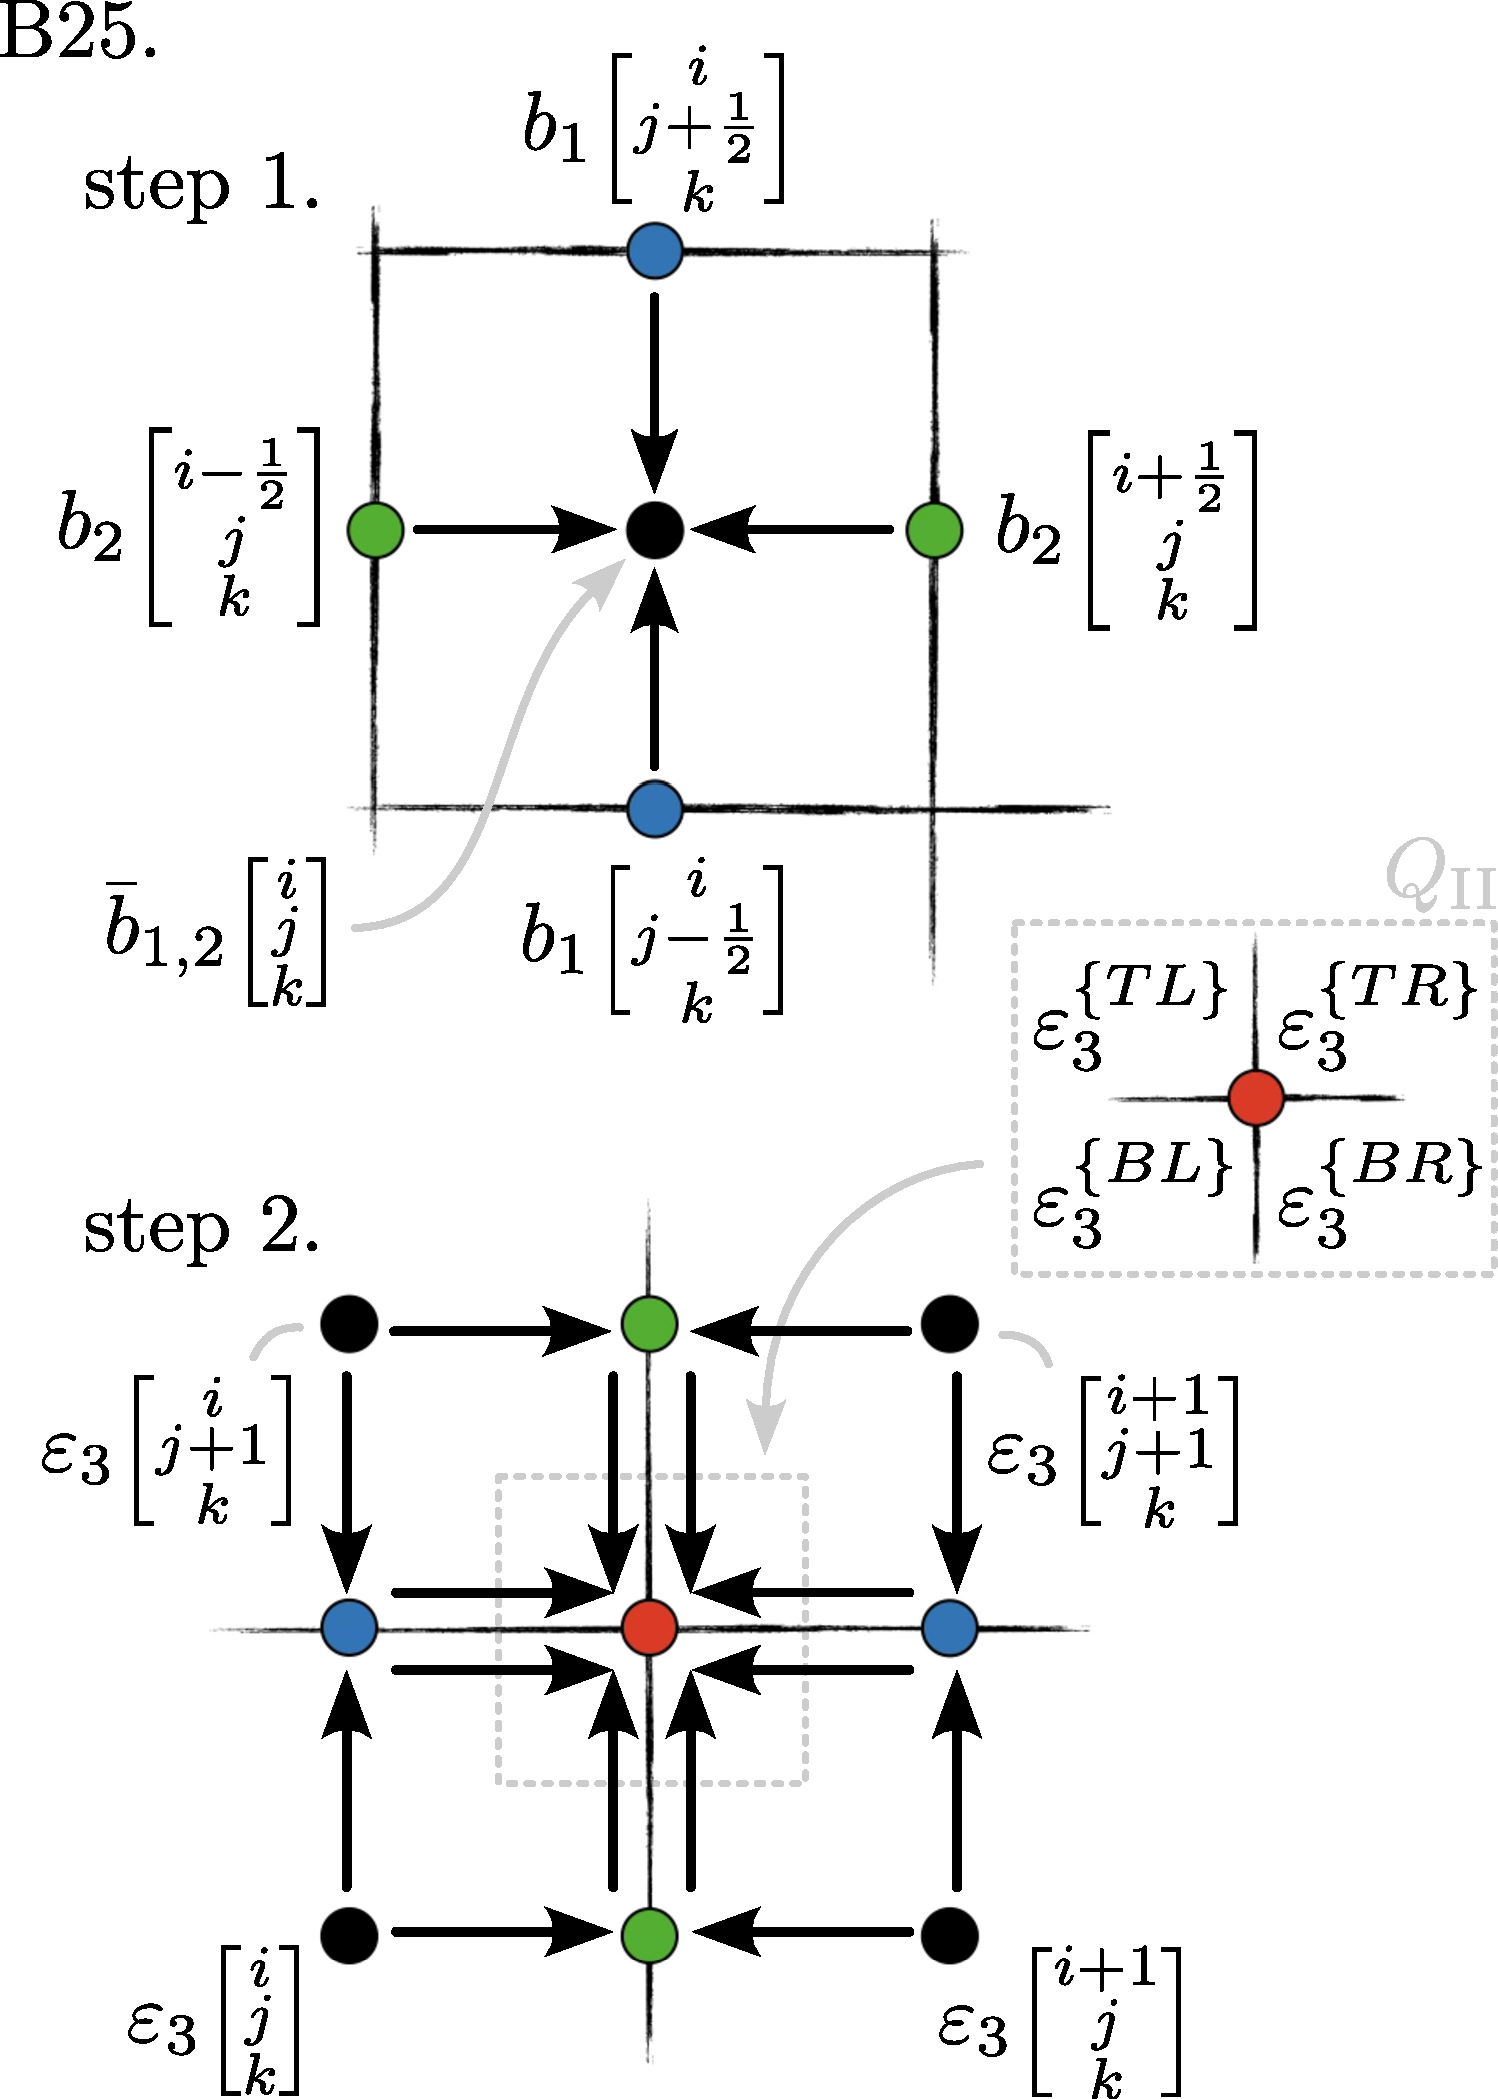
\includegraphics[width=0.65\linewidth]{figures/quokka-mhd/schematics/B25.pdf}
%DIFDELCMD <     %%%
\DIFdelendFL \DIFaddbeginFL 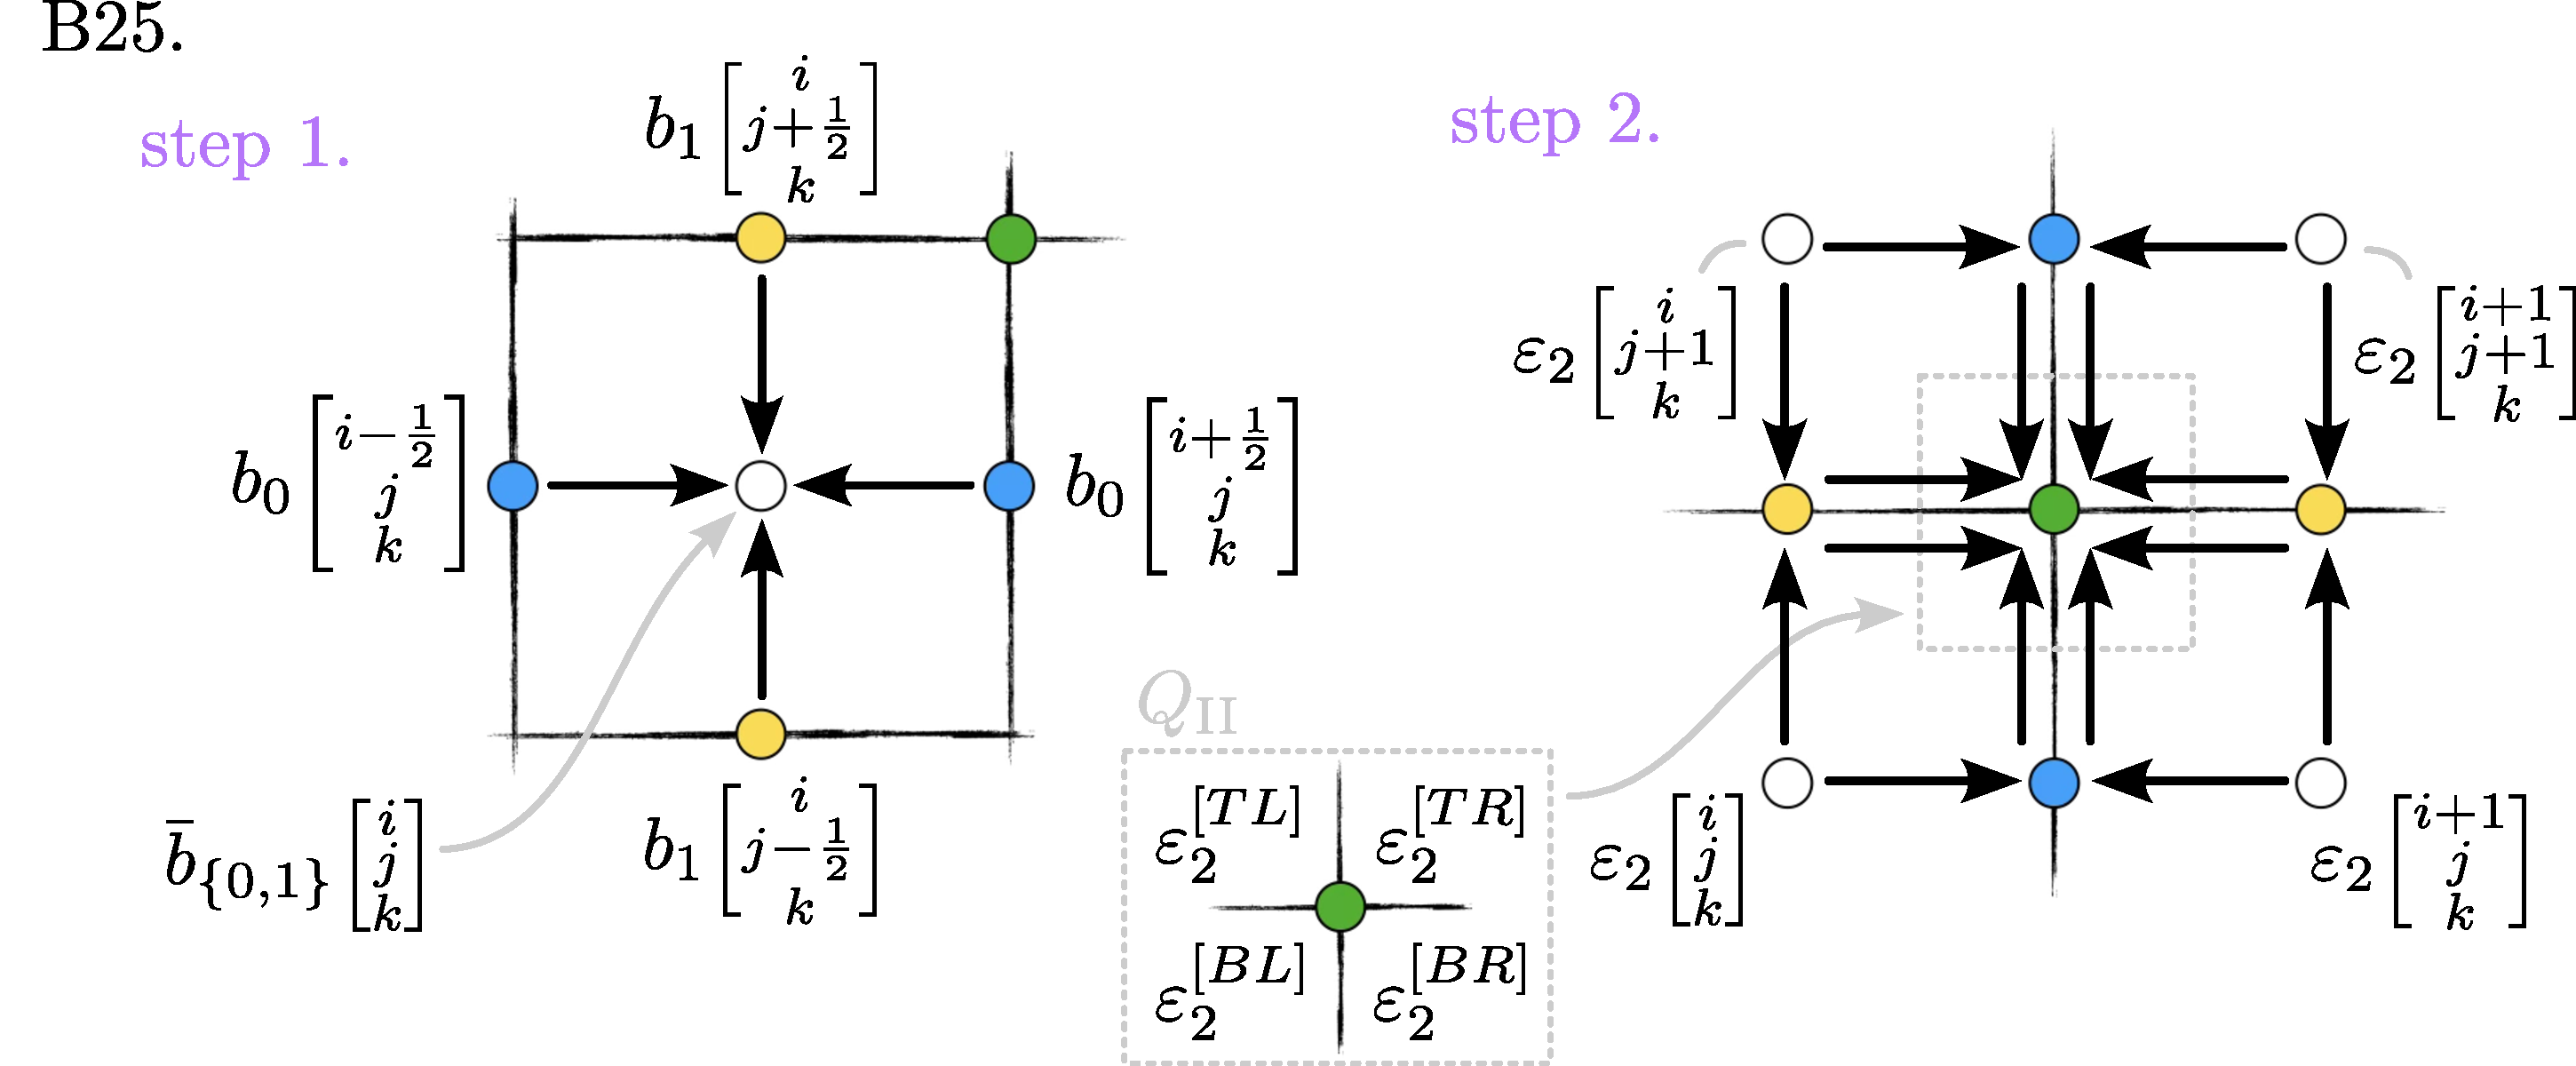
\includegraphics[width=\linewidth]{figures/quokka-mhd/schematics/b25.pdf}
    \DIFaddendFL \caption{\DIFdelbeginFL \DIFdelFL{Schematic representation of }\DIFdelendFL \DIFaddbeginFL \DIFaddFL{Two-step EMF construction for }\DIFaddendFL the \citetalias{Balsara25a} \DIFdelbeginFL \DIFdelFL{EMF reconstruction }\DIFdelendFL \DIFaddbeginFL \DIFaddFL{compute }\DIFaddendFL scheme\DIFdelbeginFL \DIFdelFL{. In the first step, the magnetic field components $b_1$ }\DIFdelendFL \DIFaddbeginFL \DIFaddFL{: $b_0$ }\DIFaddendFL and \DIFdelbeginFL \DIFdelFL{$b_2$ stored at the $x_1$ and $x_2$ cell faces }\DIFdelendFL \DIFaddbeginFL \DIFaddFL{$b_1$ }\DIFaddendFL (\DIFdelbeginFL \DIFdelFL{green and }\DIFdelendFL blue \DIFaddbeginFL \DIFaddFL{and yellow }\DIFaddendFL points) are averaged to the cell centre (\DIFdelbeginFL \DIFdelFL{black }\DIFdelendFL \DIFaddbeginFL \DIFaddFL{white }\DIFaddendFL point) \DIFdelbeginFL \DIFdelFL{, yielding mean magnetic fields $\bar{b}_{1,2}$ there. These are then combined with the cell centre velocity }\DIFdelendFL to \DIFdelbeginFL \DIFdelFL{get a cell-centre EMF component $\epsilon_3$. In the second step, this EMF component is interpolated to the cell edge }\DIFdelendFL \DIFaddbeginFL \DIFaddFL{compute $\varepsilon_2$ there }\DIFaddendFL (\DIFdelbeginFL \DIFdelFL{red point}\DIFdelendFL \DIFaddbeginFL \DIFaddFL{\mbox{%DIFAUXCMD
\cref{eqn:emf:b25a-b-avg,eqn:emf:b25a-emf-centre}}\hskip0pt%DIFAUXCMD
}\DIFaddendFL )\DIFdelbeginFL \DIFdelFL{in two steps -- it is first interpolated in the $x_1$ }\DIFdelendFL \DIFaddbeginFL \DIFaddFL{, }\DIFaddendFL and \DIFdelbeginFL \DIFdelFL{$x_2$ directions }\DIFdelendFL \DIFaddbeginFL \DIFaddFL{then reconstructed }\DIFaddendFL to the cell \DIFdelbeginFL \DIFdelFL{faces }\DIFdelendFL \DIFaddbeginFL \DIFaddFL{edge }\DIFaddendFL (\DIFdelbeginFL \DIFdelFL{blue and }\DIFdelendFL green \DIFdelbeginFL \DIFdelFL{points}\DIFdelendFL \DIFaddbeginFL \DIFaddFL{point}\DIFaddendFL ), \DIFdelbeginFL \DIFdelFL{then in the $x_2$ and $x_1$ directions to the cell edge. The two interpolation orderings are averaged to produce mean EMF $\bar{\epsilon}_3$. This procedure happens in all four corners of the cell, }\DIFdelendFL yielding four \DIFdelbeginFL \DIFdelFL{EMF }\DIFdelendFL estimates \DIFdelbeginFL \DIFdelFL{$\bar{\varepsilon}_3^{Q_\mathrm{II}}$}\DIFdelendFL \DIFaddbeginFL \DIFaddFL{$\bar{\varepsilon}_2^{[Q_\mathrm{II}]}$ (\mbox{%DIFAUXCMD
\cref{eqn:emf:b25a-average}}\hskip0pt%DIFAUXCMD
).}\DIFaddendFL }
    \label{fig:schematic:b25}
\end{figure}

\DIFdelbegin \paragraph{\DIFdel{The \mbox{%DIFAUXCMD
\citet[hereafter \citetalias{Balsara25a}]{Balsara25a} }\hskip0pt%DIFAUXCMD
strategy.}}
%DIFAUXCMD
\addtocounter{paragraph}{-1}%DIFAUXCMD
\DIFdel{In this strategy, which is illustrated in }%DIFDELCMD < \autoref{fig:schematic:b25}%%%
\DIFdelend \DIFaddbegin \DIFadd{Following the \mbox{%DIFAUXCMD
\citeauthor{Balsara25a} }\hskip0pt%DIFAUXCMD
(2025, hereafter \mbox{%DIFAUXCMD
\citetalias{Balsara25a}}\hskip0pt%DIFAUXCMD
) scheme, illustrated in \mbox{%DIFAUXCMD
\cref{fig:schematic:b25}}\hskip0pt%DIFAUXCMD
}\DIFaddend , we first average the face-centred magnetic fields to the cell centre, compute the EMFs from the cell-centred velocities and magnetic fields, and then \DIFdelbegin \DIFdel{interpolate the EMFs to }\DIFdelend \DIFaddbegin \DIFadd{reconstruct the EMFs at }\DIFaddend the cell edges. In detail, \DIFdelbegin \DIFdel{the steps are:
}%DIFDELCMD < \begin{enumerate}
%DIFDELCMD <     \item %%%
\DIFdel{Average the }\DIFdelend \DIFaddbegin \DIFadd{we average the }\DIFaddend face-centred magnetic fields to cell centres\DIFdelbegin \DIFdel{. Thus we compute
    }%DIFDELCMD < \begin{align*}
%DIFDELCMD <         b_1\EvalAtH{i}{j}{k}
%DIFDELCMD <             = \frac{1}{2} \Big(
%DIFDELCMD <                     b_1\EvalAtH{i + 1/2}{j}{k}
%DIFDELCMD <                         + b_1\EvalAtH{i - 1/2}{j}{k}
%DIFDELCMD <                 \Big)
%DIFDELCMD <     \end{align*}%%%
\DIFdelend \DIFaddbegin \DIFadd{,
}\begin{align}
    b_0\EvalAtV{i}{j}{k}
        = \frac{1}{2}\rbrac{
                b_0\EvalAtV{i + 1/2}{j}{k}
                + b_0\EvalAtV{i - 1/2}{j}{k}
            }
    , \label{eqn:emf:b25a-b-avg}
\end{align}\DIFaddend
and similarly for \DIFdelbegin \DIFdel{$b_2\EvalAtH{i}{j}{k}$. }%DIFDELCMD < \item %%%
\DIFdel{Evaluate the $x_3$}\DIFdelend \DIFaddbegin \DIFadd{$b_1\EvalAtH{i}{j}{k}$. We then evaluate the $x_2$}\DIFaddend -component of the cell-centred EMF\DIFdelbegin \DIFdel{as
    }%DIFDELCMD < \begin{align*}
%DIFDELCMD <         \varepsilon_3\EvalAtH{i}{j}{k}
%DIFDELCMD <             = -u_1\EvalAtH{i}{j}{k} b_2\EvalAtH{i}{j}{k}
%DIFDELCMD <                 + u_2\EvalAtH{i}{j}{k} b_1\EvalAtH{i}{j}{k}
%DIFDELCMD <         .
%DIFDELCMD <     \end{align*}%%%
\DIFdelend \DIFaddbegin \DIFadd{,
}\begin{align}
    \varepsilon_2\EvalAtV{i}{j}{k}
        = -u_0\EvalAtV{i}{j}{k} b_1\EvalAtV{i}{j}{k} + u_1\EvalAtV{i}{j}{k} b_0\EvalAtV{i}{j}{k}
    , \label{eqn:emf:b25a-emf-centre}
\end{align}\DIFaddend
\DIFdelbegin %DIFDELCMD < \item %%%
\DIFdel{Reconstruct the }\DIFdelend \DIFaddbegin

\DIFadd{We next reconstruct these }\DIFaddend cell-centred EMFs \DIFdelbegin \DIFdel{to }\DIFdelend \DIFaddbegin \DIFadd{at }\DIFaddend the cell faces\DIFdelbegin \DIFdel{. This yields $\varepsilon_{3}^{\cbrac{S_\mathrm{I}: x_1}}\EvalAtH{i \pm 1/2}{j}{k}$, $\varepsilon_{3}^{\cbrac{S_\mathrm{II}: x_2}}\EvalAtH{i}{j \pm 1/2}{k}$, where}\DIFdelend \DIFaddbegin \DIFadd{, yielding $\varepsilon_{2}^{[S_\mathrm{I}: x_0]}\EvalAtH{i \pm 1/2}{j}{k}$ and $\varepsilon_{2}^{[S_\mathrm{II}: x_1]}\EvalAtH{i}{j \pm 1/2}{k}$, where, }\DIFaddend as in the \citetalias{Felker18a} method\DIFaddbegin \DIFadd{, }\DIFaddend the subscripts $L$ and $R$ indicate the reconstructed quantities on the left and right side of an \DIFdelbegin \DIFdel{$x_1$}\DIFdelend \DIFaddbegin \DIFadd{$x_0$}\DIFaddend -face, $B$ and $T$ indicate the bottom and top of a \DIFdelbegin \DIFdel{$x_2$}\DIFdelend \DIFaddbegin \DIFadd{$x_1$}\DIFaddend -face, and the superscripts \DIFdelbegin \DIFdel{$x_1$ and $x_2$ }\DIFdelend \DIFaddbegin \DIFadd{$x_0$ and $x_1$ }\DIFaddend indicate the direction of reconstruction used to produce that quantity. \DIFdelbegin %DIFDELCMD < \item %%%
\DIFdel{Reconstruct the }\DIFdelend \DIFaddbegin \DIFadd{We then reconstruct these }\DIFaddend face-centred EMFs \DIFdelbegin \DIFdel{to cell edges. In this step we reconstruct }\DIFdelend \DIFaddbegin \DIFadd{at the cell edges, in }\DIFaddend the $x_1$\DIFaddbegin \DIFadd{-direction for the $x_0$}\DIFaddend -face-centred EMF \DIFdelbegin \DIFdel{in the $x_2$}\DIFdelend \DIFaddbegin \DIFadd{and in the $x_0$}\DIFaddend -direction \DIFdelbegin \DIFdel{and the $x_2$}\DIFdelend \DIFaddbegin \DIFadd{for the $x_1$}\DIFaddend -face-centred EMF\DIFdelbegin \DIFdel{in the $x_1$ direction. This yields }\DIFdelend \DIFaddbegin \DIFadd{, yielding }\DIFaddend eight estimates of each EMF at the edge, which we denote \DIFdelbegin \DIFdel{$\varepsilon_{3}^{\cbrac{Q_\mathrm{II}: x_1 x_2}}\EvalAtH{i \pm 1/2}{j \pm 1/2}{k}$ and $\varepsilon_{3}^{\cbrac{Q_\mathrm{II}: x_2 x_1}}\EvalAtH{i \pm 1/2}{j \pm 1/2}{k}$, where}\DIFdelend \DIFaddbegin \DIFadd{$\varepsilon_{2}^{[Q_\mathrm{II}: x_0 x_1]}\EvalAtH{i \pm 1/2}{j \pm 1/2}{k}$ and $\varepsilon_{2}^{[Q_\mathrm{II}: x_1 x_0]}\EvalAtH{i \pm 1/2}{j \pm 1/2}{k}$, where, as before, the superscripts $x_0 x_1$ and $x_1 x_0$ indicate }\DIFaddend the \DIFdelbegin \DIFdel{superscripts $x_1 x_2$ and $x_2 x_1$ indicate whether we reconstructed first in the $x_1$ and then the $x_2$ direction, or the reverse.
    }%DIFDELCMD < \item %%%
\DIFdel{Average over reconstruction orderings.
}\DIFdelend \DIFaddbegin \DIFadd{reconstruction order.
}

\DIFaddend As in the \citetalias{Felker18a} method, we have two estimates for each of the four corners LB, RB, LT, and RT, resulting from the two possible orderings of the \DIFdelbegin \DIFdel{one-dimensional }\DIFdelend \DIFaddbegin \DIFadd{1D }\DIFaddend reconstructions. We \DIFdelbegin \DIFdel{now }\DIFdelend average these two orderings,
\DIFdelbegin \DIFdel{yielding $\varepsilon_{3}^{\cbrac{Q_\mathrm{II}}}\EvalAtH{i \pm 1/2}{j \pm 1/2}{k} = (\varepsilon_{3}^{\cbrac{Q_\mathrm{II}: x_1 x_2}}\EvalAtH{i \pm 1/2}{j \pm 1/2}{k} + \varepsilon_{3}^{\cbrac{Q_\mathrm{II}: x_2 x_1}}\EvalAtH{i \pm 1/2}{j \pm 1/2}{k})/2$. This leaves }\DIFdelend \DIFaddbegin \begin{align}
    \varepsilon_{2}^{[Q_\mathrm{II}]}\EvalAtV{i \pm 1/2}{j \pm 1/2}{k}
        &= \frac{1}{2}\Bigg(
            \varepsilon_{2}^{[Q_\mathrm{II}: x_0 x_1]}\EvalAtV{i \pm 1/2}{j \pm 1/2}{k}
            + \varepsilon_{2}^{[Q_\mathrm{II}: x_1 x_0]}\EvalAtV{i \pm 1/2}{j \pm 1/2}{k}
        \Bigg)
    , \label{eqn:emf:b25a-average}
\end{align}
\DIFadd{leaving }\DIFaddend the four final EMF estimates at the edge that we will combine using one of the averaging methods from \DIFdelbegin %DIFDELCMD < \autoref{sec:methods:emf:averaging}%%%
\DIFdel{.
}%DIFDELCMD < \end{enumerate}
%DIFDELCMD <     %%%
\DIFdelend \DIFaddbegin \DIFadd{\sref{sec:methods:emf:averaging}.
}\DIFaddend

Note that \DIFdelbegin \DIFdel{in the \mbox{%DIFAUXCMD
\citetalias{Balsara25a} }\hskip0pt%DIFAUXCMD
reconstruction }\DIFdelend \DIFaddbegin \DIFadd{the \mbox{%DIFAUXCMD
\citetalias{Balsara25a} }\hskip0pt%DIFAUXCMD
compute }\DIFaddend scheme does not directly make use of the face-centred magnetic fields reconstructed \DIFdelbegin \DIFdel{to }\DIFdelend \DIFaddbegin \DIFadd{at }\DIFaddend the cell edges, which we compute as a first step in all \DIFdelbegin \DIFdel{reconstruction }\DIFdelend \DIFaddbegin \DIFadd{EMF compute }\DIFaddend schemes. However, since these reconstructed magnetic fields are required for both the EMF averaging schemes described in \DIFdelbegin %DIFDELCMD < \autoref{sec:methods:emf:averaging}%%%
\DIFdelend \DIFaddbegin \DIFadd{\sref{sec:methods:emf:averaging}}\DIFaddend , we carry out this step anyway.

\begin{figure}
    \centering
    \DIFdelbeginFL %DIFDELCMD < 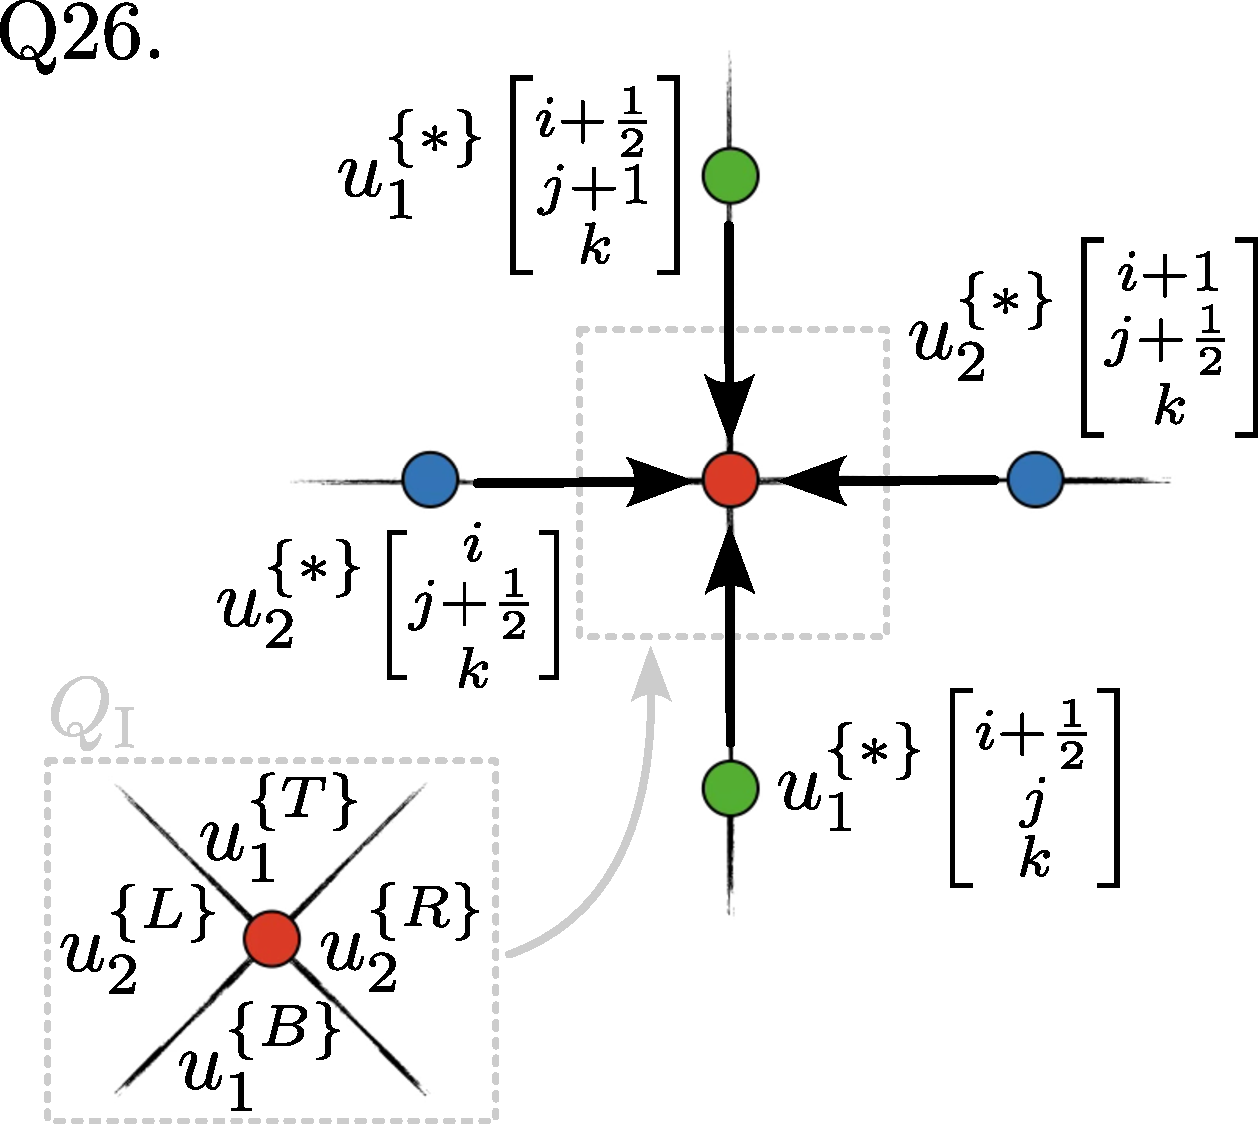
\includegraphics[width=0.6\linewidth]{figures/quokka-mhd/schematics/u-Q26.pdf}
%DIFDELCMD <     %%%
\DIFdelendFL \DIFaddbeginFL 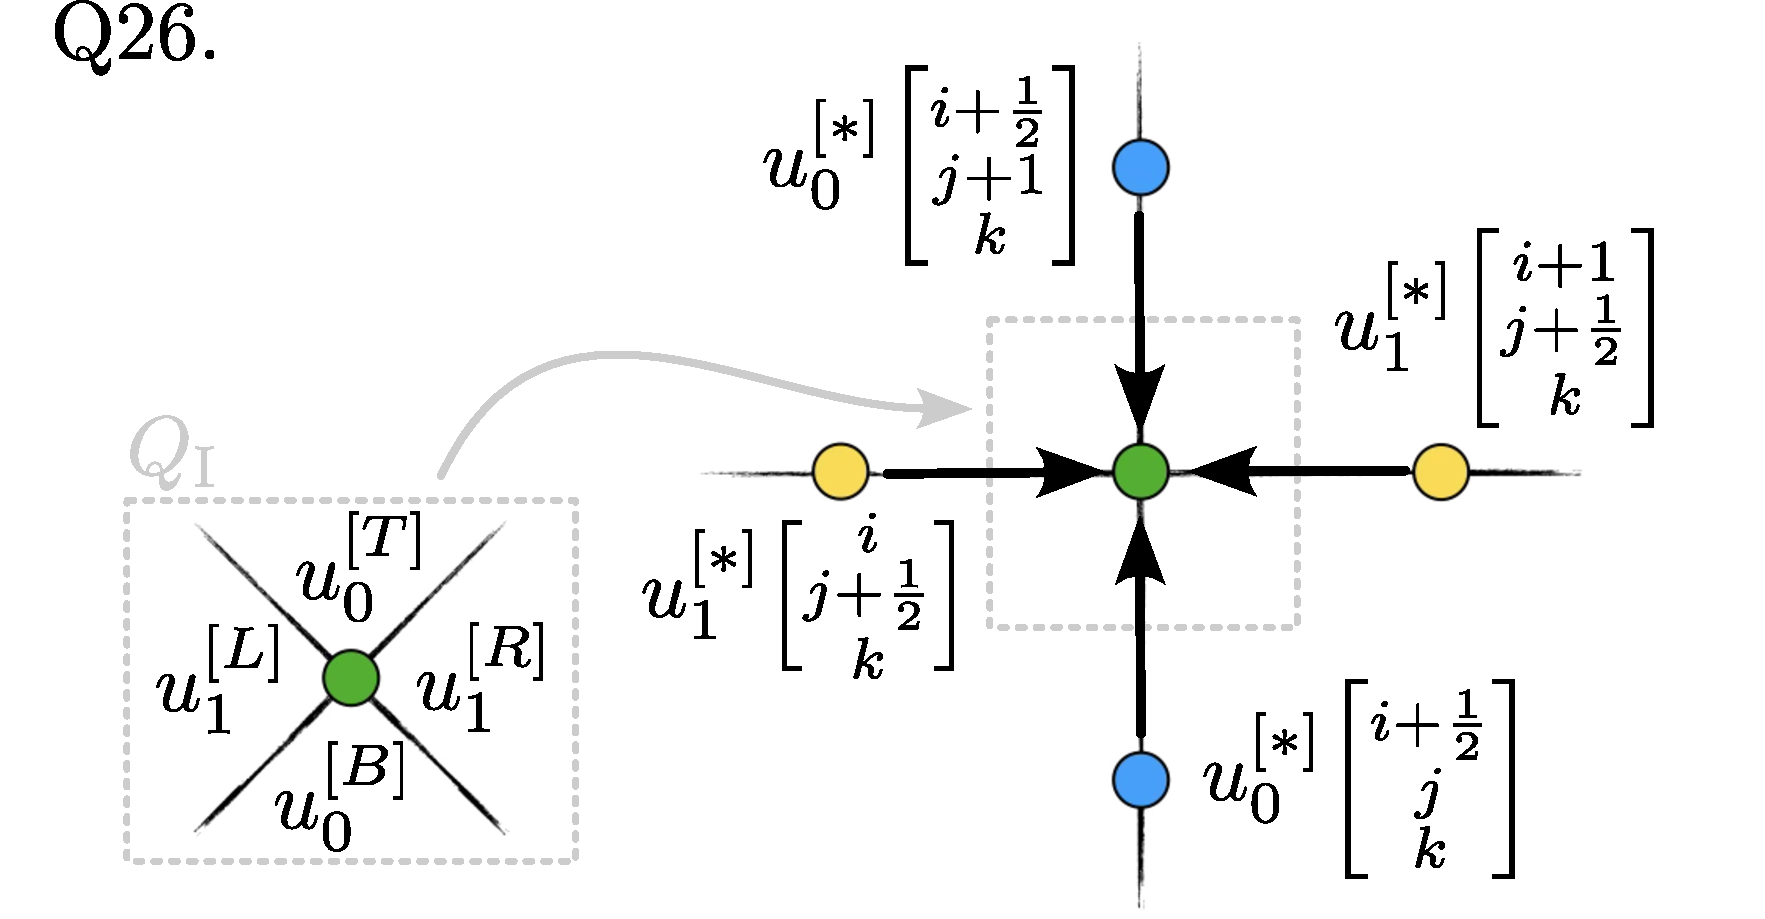
\includegraphics[width=0.65\linewidth]{figures/quokka-mhd/schematics/u-q26.pdf}
    \DIFaddendFL \caption{\DIFdelbeginFL \DIFdelFL{Schematic representation of }\DIFdelendFL \DIFaddbeginFL \DIFaddFL{Velocity reconstruction for }\DIFaddendFL the \DIFdelbeginFL \DIFdelFL{velocity interpolation part of the }\DIFdelendFL Q26 EMF \DIFdelbeginFL \DIFdelFL{reconstruction }\DIFdelendFL \DIFaddbeginFL \DIFaddFL{compute }\DIFaddendFL scheme. \DIFdelbeginFL \DIFdelFL{The scheme starts }\DIFdelendFL \DIFaddbeginFL \DIFaddFL{Starting }\DIFaddendFL from \DIFdelbeginFL \DIFdelFL{the face }\DIFdelendFL \DIFaddbeginFL \DIFaddFL{face-normal }\DIFaddendFL velocities \DIFdelbeginFL \DIFdelFL{derived from the Riemann solver mass flux }\DIFdelendFL \DIFaddbeginFL \DIFaddFL{$u_0^{[*]}$ }\DIFaddendFL and \DIFdelbeginFL \DIFdelFL{upwind density, which we denote $u_1^{\cbrac{*}}$ and $u_2^{\cbrac{*}}$, }\DIFdelendFL \DIFaddbeginFL \DIFaddFL{$u_1^{[*]}$ (\mbox{%DIFAUXCMD
\cref{eqn:emf:q26-facevel}}\hskip0pt%DIFAUXCMD
) }\DIFaddendFL at the \DIFdelbeginFL \DIFdelFL{$x_1$ }\DIFdelendFL \DIFaddbeginFL \DIFaddFL{$x_0$ }\DIFaddendFL and \DIFdelbeginFL \DIFdelFL{$x_2$ }\DIFdelendFL \DIFaddbeginFL \DIFaddFL{$x_1$ }\DIFaddendFL cell faces (blue and \DIFdelbeginFL \DIFdelFL{green }\DIFdelendFL \DIFaddbeginFL \DIFaddFL{yellow }\DIFaddendFL points)\DIFdelbeginFL \DIFdelFL{. These }\DIFdelendFL \DIFaddbeginFL \DIFaddFL{, these }\DIFaddendFL are \DIFdelbeginFL \DIFdelFL{then interpolated to }\DIFdelendFL \DIFaddbeginFL \DIFaddFL{reconstructed at }\DIFaddendFL the cell edge (\DIFdelbeginFL \DIFdelFL{red }\DIFdelendFL \DIFaddbeginFL \DIFaddFL{green }\DIFaddendFL point) \DIFdelbeginFL \DIFdelFL{, yielding estimates $u_1^{\{B\}}$ }\DIFdelendFL \DIFaddbeginFL \DIFaddFL{to yield $u_0^{[B]}$ }\DIFaddendFL and \DIFdelbeginFL \DIFdelFL{$u_1^{\{T\}}$ for the velocity in the $x_1$ direction}\DIFdelendFL \DIFaddbeginFL \DIFaddFL{$u_0^{[T]}$}\DIFaddendFL , and \DIFdelbeginFL \DIFdelFL{$u_2^{\{L\}}$ }\DIFdelendFL \DIFaddbeginFL \DIFaddFL{$u_1^{[L]}$ }\DIFaddendFL and \DIFdelbeginFL \DIFdelFL{$u_2^{\{R\}}$ for the velocity in the $x_2$ direction}\DIFdelendFL \DIFaddbeginFL \DIFaddFL{$u_1^{[R]}$}\DIFaddendFL . These \DIFdelbeginFL \DIFdelFL{are then combined }\DIFdelendFL \DIFaddbeginFL \DIFaddFL{combine }\DIFaddendFL with the \DIFdelbeginFL \DIFdelFL{interpolated }\DIFdelendFL magnetic fields \DIFaddbeginFL \DIFaddFL{reconstructed at the edge }\DIFaddendFL (\DIFdelbeginFL %DIFDELCMD < \autoref{fig:schematic:b-common} %%%
\DIFdelendFL \DIFaddbeginFL \DIFaddFL{\mbox{%DIFAUXCMD
\cref{fig:schematic:b-common}}\hskip0pt%DIFAUXCMD
) }\DIFaddendFL to yield \DIFdelbeginFL \DIFdelFL{an estimate of }\DIFdelendFL the \DIFdelbeginFL \DIFdelFL{cell edge }\DIFdelendFL EMF (\DIFdelbeginFL %DIFDELCMD < \autoref{eqn:emf:q26}%%%
\DIFdelendFL \DIFaddbeginFL \DIFaddFL{\mbox{%DIFAUXCMD
\cref{eqn:emf:q26}}\hskip0pt%DIFAUXCMD
}\DIFaddendFL ).}
    \label{fig:schematic:q26}
\end{figure}

\DIFdelbegin \paragraph{\DIFdel{The Quokka 2026 (Q26) strategy.}} %DIFAUXCMD
\addtocounter{paragraph}{-1}%DIFAUXCMD
\DIFdel{The final strategy }\DIFdelend \DIFaddbegin \DIFadd{We refer to the final scheme }\DIFaddend that we consider \DIFdelbegin \DIFdel{, illustrated in }%DIFDELCMD < \autoref{fig:schematic:q26}%%%
\DIFdel{, is new, though it is similar in spirit to an approach taken }\DIFdelend \DIFaddbegin \DIFadd{as the Quokka 2026 (Q26) scheme. Illustrated in \mbox{%DIFAUXCMD
\cref{fig:schematic:q26}}\hskip0pt%DIFAUXCMD
, it is a modified version of an approach inspired }\DIFaddend by \citet{Mignone21a}. As with the \citetalias{Felker18a} method, we \DIFdelbegin \DIFdel{bring }\DIFdelend \DIFaddbegin \DIFadd{independently reconstruct }\DIFaddend the velocity and magnetic field \DIFdelbegin \DIFdel{to }\DIFdelend \DIFaddbegin \DIFadd{at }\DIFaddend the cell edge\DIFdelbegin \DIFdel{separately }\DIFdelend \DIFaddbegin \DIFadd{, }\DIFaddend and combine them there to compute the EMF, but with an important difference: rather than reconstructing velocities \DIFaddbegin \DIFadd{at the face }\DIFaddend from the cell centre \DIFdelbegin \DIFdel{to the face and then }\DIFdelend \DIFaddbegin \DIFadd{and then at the edge }\DIFaddend from the face\DIFdelbegin \DIFdel{to the edge}\DIFdelend , we instead begin from face velocities obtained directly from the \DIFdelbegin \DIFdel{Riemann solver (}%DIFDELCMD < \autoref{sec:methods:flux}%%%
\DIFdel{). Specifically, we obtain a velocity at each face by dividing the mass flux returned by the Riemann solver by the left or right state density, depending on which is the upwind direction at that face. We denote the velocities }\DIFdelend \DIFaddbegin \DIFadd{flux calculation (\sref{sec:methods:flux}), and therefore only require a single reconstruction to reach cell edges.}\footnote{
    \DIFadd{We originally attempted to compute the face velocity by dividing the mass flux returned by the Riemann solver by the upwind-state density, but found that this was unstable for the complex magnetic field geometries resolved in high-resolution, turbulent systems such as the Orszag-Tang vortex and the current sheet tested later in this chapter.
}} \DIFadd{We estimate this face-normal velocity, which we denote $u_{0}^{[*]}\EvalAtH{i \pm 1/2}{j}{k}$ on the $x_0$-faces (and similarly $u_1^{[*]}\EvalAtH{i}{j \pm 1/2}{k}$ }\DIFaddend on the $x_1$\DIFdelbegin \DIFdel{- and $x_2$}\DIFdelend -faces\DIFdelbegin \DIFdel{derived via this procedure as $u_{1}^{\cbrac{*}}\EvalAtH{i \pm 1/2}{j}{k}$ and $u_{2}^{\cbrac{*}}\EvalAtH{i}{j \pm 1/2}{k}$. This means that we start will all the quantities required to compute the EMF already stored at cell faces, and we require only a single reconstruction to reach cell edges. The steps in detail are:
}%DIFDELCMD < \begin{enumerate}
%DIFDELCMD <     \item %%%
\DIFdel{Reconstruct the face velocities to cell edges.
We reconstruct $u_{1}^{\cbrac{*}}$ in the $x_2$}\DIFdelend \DIFaddbegin \DIFadd{, }\etc\DIFadd{), via a fast-magnetosonic-wavespeed-weighted average of the reconstructed left and right normal-velocity states at the face,
}\begin{align}
    u_{0}^{[*]}
        = \frac{\alpha_0^{[+]} u_{0}^{[L]} + \alpha_0^{[-]} u_{0}^{[R]}}{\alpha_0^{[+]} + \alpha_0^{[-]}}
    , \label{eqn:emf:q26-facevel}
\end{align}
\DIFadd{where every quantity in this equation is evaluated at the shared face $\EvalAtH{i + 1/2}{j}{k}$, and $u_0^{[L]}$ and $u_0^{[R]}$ are the reconstructed left and right states of the normal velocity component. Following \mbox{%DIFAUXCMD
\citet{Miyoshi05a} }\hskip0pt%DIFAUXCMD
(their eqn. 67), we estimate the non-negative bounding wavespeeds of the Riemann fan at the $x_0$-face as
}\begin{align}
    \alpha_0^{[+]}
        &= \max\sbrac{0,\ \max\sbrac{u_0^{[L]}, u_0^{[R]}} + \max\sbrac{c_\mathrm{fm}^{[L]}, c_\mathrm{fm}^{[R]}}}
    \\
    \alpha_0^{[-]}
        &= \max\sbrac{0,\ \max\sbrac{c_\mathrm{fm}^{[L]}, c_\mathrm{fm}^{[R]}} - \min\sbrac{u_0^{[L]}, u_0^{[R]}}}
    , \label{eqn:emf:alpha-pm}
\end{align}
\DIFadd{where $c_\mathrm{fm}^{[L]}$ and $c_\mathrm{fm}^{[R]}$ are the fast-magnetosonic speed (\sref{sec:scheme-comparison:waves:fast}) evaluated at the reconstructed left and right states; we use these same face-level quantities, maximised over the faces adjacent to each edge (\mbox{%DIFAUXCMD
\cref{eqn:emf:alpha-edge}}\hskip0pt%DIFAUXCMD
), for EMF averaging in \sref{sec:methods:emf:averaging}. The wavespeed averaging we use here is the same as that proposed in equation 29 of \mbox{%DIFAUXCMD
\citet{Mignone21a}}\hskip0pt%DIFAUXCMD
, but here we apply it to the normal component of the velocity rather than to the transverse components as in their work.
}

\DIFadd{Once we have computed the face velocities $u_0^{[*]}$ and $u_1^{[*]}$, we reconstruct $u_{0}^{[*]}$ in the $x_1$}\DIFaddend -direction to yield \DIFdelbegin \DIFdel{$u_{1}^{\cbrac{*;S_\mathrm{II}}}\EvalAtH{i \pm 1/2}{j \pm 1/2}{k}$}\DIFdelend \DIFaddbegin \DIFadd{$u_{0}^{[*;S_\mathrm{II}]}\EvalAtH{i \pm 1/2}{j \pm 1/2}{k}$}\DIFaddend , and reconstruct \DIFdelbegin \DIFdel{$u_{2}^{\cbrac{*}}$ in the $x_1$}\DIFdelend \DIFaddbegin \DIFadd{$u_{1}^{[*]}$ in the $x_0$}\DIFaddend -direction to yield \DIFdelbegin \DIFdel{$u_{2}^{\cbrac{*;S_\mathrm{I}}}\EvalAtH{i \pm 1/2}{j \pm 1/2}{k}$. As }\DIFdelend \DIFaddbegin \DIFadd{$u_{1}^{[*;S_\mathrm{I}]}\EvalAtH{i \pm 1/2}{j \pm 1/2}{k}$, where, as }\DIFaddend previously, $L$, $R$, $T$, and $B$ indicate states on the left, right, top, and bottom of the edge. \DIFdelbegin %DIFDELCMD < \item %%%
\DIFdel{Compute the EMFs at the edges. }\DIFdelend For the $x_2$ edges, we can \DIFaddbegin \DIFadd{then }\DIFaddend compute four estimates of the EMF as
\DIFdelbegin \DIFdel{:
}%DIFDELCMD < \begin{align}
%DIFDELCMD <     &\varepsilon_{3}^{\{Q_\mathrm{II}\}}\EvalAtH{i \pm 1/2}{j \pm 1/2}{k}
%DIFDELCMD <         = -u_{1}^{\cbrac{*;S_\mathrm{II}}}\EvalAtH{i \pm 1/2}{j \pm 1/2}{k}
%DIFDELCMD <             b_{2}^{\cbrac{S_\mathrm{I}}}\EvalAtH{i \pm 1/2}{j \pm 1/2}{k}
%DIFDELCMD <         \nonumber \\
%DIFDELCMD <         &\nquad[7] + u_{2}^{\cbrac{*;S_\mathrm{I}}}\EvalAtH{i \pm 1/2}{j \pm 1/2}{k}
%DIFDELCMD <             b_{1}^{\cbrac{S_\mathrm{II}}}\EvalAtH{i \pm 1/2}{j \pm 1/2}{k}
%DIFDELCMD <     , \label{eqn:emf:q26}
%DIFDELCMD < \end{align}%%%
\DIFdelend \DIFaddbegin \begin{align}
    \varepsilon_{2}^{[Q_\mathrm{II}]}\EvalAtV{i \pm 1/2}{j \pm 1/2}{k}
        &= -u_{0}^{[*;S_\mathrm{II}]}\EvalAtV{i \pm 1/2}{j \pm 1/2}{k}
            b_{1}^{[S_\mathrm{I}]}\EvalAtV{i \pm 1/2}{j \pm 1/2}{k}
        \nonumber \\
        &\nquad[1]
            + u_{1}^{[*;S_\mathrm{I}]}\EvalAtV{i \pm 1/2}{j \pm 1/2}{k}
            b_{0}^{[S_\mathrm{II}]}\EvalAtV{i \pm 1/2}{j \pm 1/2}{k}
    , \label{eqn:emf:q26}
\end{align}\DIFaddend
where \DIFdelbegin \DIFdel{$S_\mathrm{I}$ can be either $L$ or $R$, and $S_\mathrm{II}$ can be either $B$ or $T$}\DIFdelend \DIFaddbegin \DIFadd{$S_\mathrm{I} \in \cbrac{L, R}$ and $S_\mathrm{II} \in \cbrac{T, B}$, and $Q_\mathrm{II}$, the quadrant label of each corner estimate, is given by the concatenation $S_\mathrm{I} S_\mathrm{II}$}\DIFaddend . These are the four quadrant estimates on which our EMF averaging scheme will act.
\DIFdelbegin %DIFDELCMD < \end{enumerate}
%DIFDELCMD < %%%
\DIFdelend

In comparison to the \citetalias{Felker18a} and \citetalias{Balsara25a} schemes, it is clear that the Q26 scheme involves significantly fewer reconstructions and fewer temporary variables. However, this is partially offset by an increase in the cost of the flux calculation associated with ghost zones. For reasons we discuss in \DIFdelbegin %DIFDELCMD < \autoref{sec:methods:emf:averaging}%%%
\DIFdelend \DIFaddbegin \DIFadd{\sref{sec:methods:emf:averaging}}\DIFaddend , our EMF averaging schemes require that we calculate the fluxes not just in the real cells of the domain, but \DIFdelbegin \DIFdel{for }\DIFdelend \DIFaddbegin \DIFadd{also for at least }\DIFaddend one ghost cell. The Q26 scheme in general requires more, at least if we wish to use a higher-order reconstruction method: we must be able to reconstruct \DIFdelbegin \DIFdel{$u_{1}^{\cbrac{*}}$ in the $x_2$}\DIFdelend \DIFaddbegin \DIFadd{$u_{0}^{[*]}$ in the $x_1$}\DIFaddend -direction, which requires knowledge of the star state not just at the one ghost face adjacent to the real cells, but in two ghost zones for PLM \DIFdelbegin \DIFdel{interpolation}\DIFdelend \DIFaddbegin \DIFadd{reconstruction}\DIFaddend , and three for PPM or PPM-EP. We are therefore required to solve the Riemann problem in this many more ghost zones. We will test the performance impact of this trade-off \DIFdelbegin \DIFdel{-- }\DIFdelend \DIFaddbegin \DIFadd{(}\DIFaddend fewer reconstruction steps but more ghost zones\DIFdelbegin \DIFdel{-- in }%DIFDELCMD < \autoref{sec:performance}%%%
\DIFdelend \DIFaddbegin \DIFadd{) in \sref{sec:scheme-comparisons}}\DIFaddend .

\subsubsection{The EMF averaging scheme}
\label{sec:methods:emf:averaging}

Each of the \DIFdelbegin \DIFdel{reconstruction }\DIFdelend \DIFaddbegin \DIFadd{EMF compute }\DIFaddend schemes described in \DIFdelbegin %DIFDELCMD < \autoref{sec:methods:emf:reconstruction} %%%
\DIFdel{yields estimates }\DIFdelend \DIFaddbegin \DIFadd{\sref{sec:methods:emf:compute} yields four quadrant-estimates }\DIFaddend of the EMF around each corner of the cell edge; for the \DIFdelbegin \DIFdel{$x_3$}\DIFdelend \DIFaddbegin \DIFadd{$x_2$}\DIFaddend -edges, these are denoted \DIFdelbegin \DIFdel{$\varepsilon_{3}^{\{Q_\mathrm{II}\}}\EvalAtH{i \pm 1/2}{j \pm 1/2}{k}$}\DIFdelend \DIFaddbegin \DIFadd{$\varepsilon_{2}^{[Q_\mathrm{II}]}\EvalAtH{i \pm 1/2}{j \pm 1/2}{k}$}\DIFaddend . The final step is to average these together to yield a single estimate of the EMF, \DIFdelbegin \DIFdel{$\varepsilon_{3}\EvalAtH{i \pm 1/2}{j \pm 1/2}{k}$. We consider two schemes }\DIFdelend \DIFaddbegin \DIFadd{$\varepsilon_{2}\EvalAtH{i \pm 1/2}{j \pm 1/2}{k}$, at the edge. Below we describe the two schemes we consider }\DIFaddend for doing so\DIFdelbegin \DIFdel{below.
In addition to the EMFs, these schemes make use of }\DIFdelend \DIFaddbegin \DIFadd{.
}

\DIFadd{Both schemes also require }\DIFaddend the magnetic fields reconstructed \DIFdelbegin \DIFdel{to }\DIFdelend \DIFaddbegin \DIFadd{at }\DIFaddend the cell edges, \DIFdelbegin \DIFdel{$b_{1}^{\cbrac{S_\mathrm{II}}}\EvalAtH{i \pm 1/2}{j \pm 1/2}{k}$ and $b_{2}^{\cbrac{S_\mathrm{I}}}\EvalAtH{i \pm 1/2}{j \pm 1/2}{k}$}\DIFdelend \DIFaddbegin \DIFadd{$b_{0}^{[S_\mathrm{II}]}\EvalAtH{i \pm 1/2}{j \pm 1/2}{k}$ and $b_{1}^{[S_\mathrm{I}]}\EvalAtH{i \pm 1/2}{j \pm 1/2}{k}$}\DIFaddend , and the \DIFdelbegin \DIFdel{minimum and maximum wavespeeds on the four }\DIFdelend \DIFaddbegin \DIFadd{wavespeed magnitudes at the edge, taken as the maximum of the corresponding face-level magnitudes (\sref{sec:methods:emf:compute}) on the two }\DIFaddend faces adjacent to \DIFdelbegin \DIFdel{the edgeas computed during the flux update. We denote these wavespeeds $\alpha_{1,2}^{\cbrac{\pm}}$,
where $x_1$ or $x_2$ indicates the direction of the face across which the speed is calculated, and $\pm$ indicates the minimum (most negative) or maximum wavespeed. We compute $\alpha_{1,2}^{\cbrac{\pm}}$ following the procedure outlined in Appendix A of \mbox{%DIFAUXCMD
\citetalias{Felker18a}}\hskip0pt%DIFAUXCMD
. }\DIFdelend \DIFaddbegin \DIFadd{that edge,
}\begin{align}
    \alpha_0^{[\pm]}\EvalAtV{i + 1/2}{j + 1/2}{k}
        &= \max\sbrac{
            \alpha_0^{[\pm]}\EvalAtV{i + 1/2}{j}{k},
            \alpha_0^{[\pm]}\EvalAtV{i + 1/2}{j + 1}{k}
        }
    , \label{eqn:emf:alpha-edge}
\end{align}
\DIFadd{and analogously for $\alpha_1^{[\pm]}$ by cyclic permutation. }\DIFaddend Note that computing these wavespeeds requires that we solve the Riemann problem not just over the real cells of the domain, but for one ghost cell as well.

\DIFdelbegin \paragraph{\DIFdel{The \mbox{%DIFAUXCMD
\citet[hereafter \citetalias{Londrillo04a}]{Londrillo04a} }\hskip0pt%DIFAUXCMD
strategy.}}
%DIFAUXCMD
\addtocounter{paragraph}{-1}%DIFAUXCMD
\DIFdel{Our first option }\DIFdelend \DIFaddbegin \DIFadd{Our first scheme, following the \mbox{%DIFAUXCMD
\citet[hereafter \citetalias{Londrillo04a}]{Londrillo04a} }\hskip0pt%DIFAUXCMD
approach, }\DIFaddend combines the four corner EMFs using the solution to a 2D HLL Riemann solver\DIFdelbegin \DIFdel{, following the approach developed by \mbox{%DIFAUXCMD
\citetalias{Londrillo04a}}\hskip0pt%DIFAUXCMD
}\DIFdelend . Our exact implementation of this solution is given by equation 41 of \citetalias{Felker18a}\DIFaddbegin \DIFadd{,
}\begin{align}
    \varepsilon_{2}\EvalAtV{i \pm 1/2}{j \pm 1/2}{k}
        &= \frac{
            \alpha_0^{[+]}\alpha_1^{[+]} \varepsilon_2^{[LB]}
                + \alpha_0^{[-]}\alpha_1^{[+]} \varepsilon_2^{[RB]}
        }{
            \rbrac{\alpha_0^{[+]}+\alpha_0^{[-]}} \rbrac{\alpha_1^{[+]}+\alpha_1^{[-]}}
        }
            + \frac{
                \alpha_0^{[+]}\alpha_1^{[-]} \varepsilon_2^{[LT]}
                + \alpha_0^{[-]}\alpha_1^{[-]} \varepsilon_2^{[RT]}
            }{
                \rbrac{\alpha_0^{[+]}+\alpha_0^{[-]}} \rbrac{\alpha_1^{[+]}+\alpha_1^{[-]}}
            }
        \nonumber \\
        &\nquad[1]
            - \frac{\alpha_1^{[+]}\alpha_1^{[-]}}{\alpha_1^{[+]}+\alpha_1^{[-]}} \rbrac{b_0^{[T]} - b_0^{[B]}}
            + \frac{\alpha_0^{[+]}\alpha_0^{[-]}}{\alpha_0^{[+]}+\alpha_0^{[-]}} \rbrac{b_1^{[R]} - b_1^{[L]}}
    , \label{eqn:emf:ld04}
\end{align}
\DIFadd{where every quantity in this equation is evaluated at the shared edge $\EvalAtH{i \pm 1/2}{j \pm 1/2}{k}$}\DIFaddend . This yields a single upwinded EMF estimate \DIFdelbegin \DIFdel{$\varepsilon_3\EvalAtH{i \pm 1/2}{j \pm 1/2}{k}$ }\DIFdelend \DIFaddbegin \DIFadd{$\varepsilon_2\EvalAtH{i \pm 1/2}{j \pm 1/2}{k}$ }\DIFaddend at each cell edge.

\DIFdelbegin \paragraph{\DIFdel{The \mbox{%DIFAUXCMD
\citet[hereafter \citetalias{Balsara25b}]{Balsara25b} }\hskip0pt%DIFAUXCMD
strategy.}}
%DIFAUXCMD
\addtocounter{paragraph}{-1}%DIFAUXCMD
\DIFdel{Our second option uses a }\DIFdelend \DIFaddbegin \DIFadd{Our second scheme uses the }\DIFaddend new 2D Riemann solver developed by \DIFdelbegin \DIFdel{\mbox{%DIFAUXCMD
\citetalias{Balsara25b} }\hskip0pt%DIFAUXCMD
}\DIFdelend \DIFaddbegin \DIFadd{\mbox{%DIFAUXCMD
\citeauthor{Balsara25b} }\hskip0pt%DIFAUXCMD
(2025, hereafter \mbox{%DIFAUXCMD
\citetalias{Balsara25b}}\hskip0pt%DIFAUXCMD
) }\DIFaddend to combine the EMFs. \DIFdelbegin \DIFdel{The implementation of this Riemann solver that we follow is given by equation 3.10 of \mbox{%DIFAUXCMD
\citetalias{Balsara25a}}\hskip0pt%DIFAUXCMD
. Note that although both this Riemann solver method and the interpolation scheme we have described as the \mbox{%DIFAUXCMD
\citetalias{Balsara25a} }\hskip0pt%DIFAUXCMD
strategy were introduced together, they are independent in the sense that }\DIFdelend \DIFaddbegin \DIFadd{Unlike \mbox{%DIFAUXCMD
\cref{eqn:emf:ld04}}\hskip0pt%DIFAUXCMD
, this cannot be expressed as a single average of the four corner EMFs: instead, depending on the signs of the one-sided wavespeeds bounding the edge, it selects among a raw corner EMF, a one-sided (single-direction) resolved state, or a fully 2D resolved state analogous to \mbox{%DIFAUXCMD
\cref{eqn:emf:ld04}}\hskip0pt%DIFAUXCMD
. We do not reproduce this full case structure here, and instead refer the reader to equations 3.2-3.10 of \mbox{%DIFAUXCMD
\citetalias{Balsara25a} }\hskip0pt%DIFAUXCMD
for its complete definition and discussion.
}

\DIFadd{The EMF averaging scheme (\mbox{%DIFAUXCMD
\citetalias{Balsara25b}}\hskip0pt%DIFAUXCMD
) and the EMF compute scheme (\mbox{%DIFAUXCMD
\citetalias{Balsara25a}}\hskip0pt%DIFAUXCMD
) are independent choices within our framework: }\DIFaddend we can apply the \citetalias{Balsara25b} Riemann solver to any combination of four corner EMFs\DIFaddbegin \DIFadd{, }\DIFaddend regardless of the \DIFdelbegin \DIFdel{reconstruction }\DIFdelend \DIFaddbegin \DIFadd{EMF compute }\DIFaddend scheme used to obtain them\DIFdelbegin \DIFdel{, and, }\DIFdelend \DIFaddbegin \DIFadd{; }\DIFaddend conversely, we are free to use the \citetalias{Londrillo04a} \DIFdelbegin \DIFdel{rather than the \mbox{%DIFAUXCMD
\citetalias{Balsara25b} }\hskip0pt%DIFAUXCMD
averaging strategy on the }\DIFdelend \DIFaddbegin \DIFadd{averaging scheme rather than \mbox{%DIFAUXCMD
\citetalias{Balsara25b} }\hskip0pt%DIFAUXCMD
on }\DIFaddend corner EMFs even if they were derived using the \citetalias{Balsara25a} \DIFdelbegin \DIFdel{reconstruction method}\DIFdelend \DIFaddbegin \DIFadd{compute scheme}\DIFaddend . Below in \DIFdelbegin %DIFDELCMD < \autoref{sec:performance} %%%
\DIFdelend \DIFaddbegin \DIFadd{\sref{sec:scheme-comparisons} }\DIFaddend we will in fact test multiple such combinations.

\subsection{\DIFdelbegin \DIFdel{Time stepping with flux correction}\DIFdelend \DIFaddbegin \DIFadd{Constant Ohmic resistivity}\DIFaddend }
\DIFdelbegin %DIFDELCMD < \label{sec:methods:time-stepping}
%DIFDELCMD < %%%
\DIFdelend \DIFaddbegin \label{sec:methods:resistivity}
\DIFaddend

\DIFdelbegin \DIFdel{Now that we have describe our method for compute the fluxes through faces and }\DIFdelend \DIFaddbegin \DIFadd{Up to this point we have described our scheme for }\DIFaddend the \DIFdelbegin \DIFdel{EMFs around cell edges , we are in a position to describe an overall time stepping scheme.
As discussed }\DIFdelend \DIFaddbegin \DIFadd{ideal MHD equations. To extend the scheme to also handle resistive MHD flows, where a controlled magnetic Reynolds number is desired, we include a constant (in space and time) Ohmic resistivity $\eta$. With this, Ohm's law becomes:
}\begin{align}
    \mVector{\varepsilon}
        &= -\mVector{u}\times\mVector{b} + \eta\, \mVector{j}
    , \label{eqn:resistivity:ohms-law}
\end{align}
\DIFadd{where $\mVector{j} = \nabla\times\mVector{b}$ is the current density in (rationalised-Gaussian units). Since $\eta\, \mVector{j}$ lives at the same edges where we already store EMFs, the resistive term acts as an explicit magnetic-diffusion source that can be incorporated directly during the existing EMF calculation in \sref{sec:methods:emf}. Doing so reuses the existing EMF calculation's kernel launches and memory footprint, and leaves the CT update (\mbox{%DIFAUXCMD
\cref{eqn:ct:circulation-update}}\hskip0pt%DIFAUXCMD
) unaffected; thus $\nabla\cdot\mVector{b} = 0$ is preserved by construction.
}

\begin{figure}
    \centering
    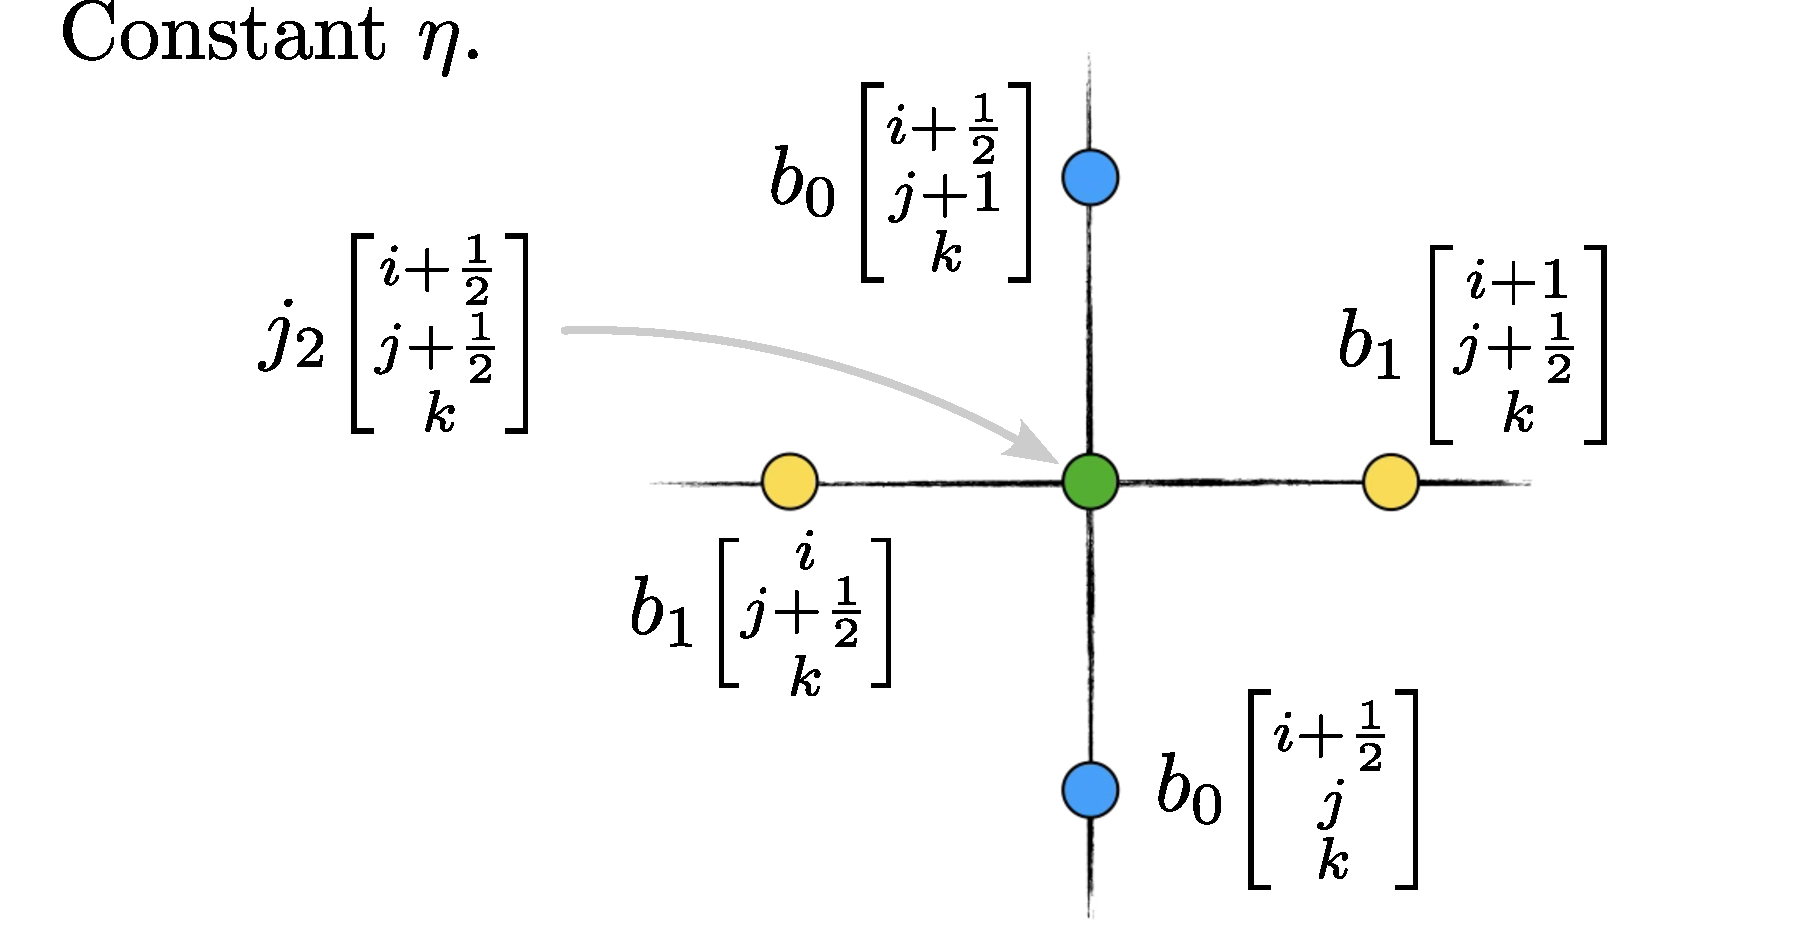
\includegraphics[width=0.65\linewidth]{figures/quokka-mhd/schematics/eta-constant.pdf}
    \caption{\DIFaddFL{The constant-$\eta$ stencil for the Ohmic contribution to the edge-centred EMF $\varepsilon_2$ (green point), constructed from the four adjacent face-centred magnetic field values: $b_0$ (blue points) and $b_1$ (yellow points) (\mbox{%DIFAUXCMD
\cref{eqn:resistivity:current-stencil}}\hskip0pt%DIFAUXCMD
). The corresponding stencils for $j_0$ and $j_1$ follow by cyclic permutation.}}
    \label{fig:schematic:eta-constant}
\end{figure}

\DIFadd{For scalar $\eta$, only the component of $\mVector{j}$ aligned with each edge enters the EMF correction. As in earlier sections, we highlight, without loss of generality, the $x_2$-edge centred at $\EvalAtH{i + 1/2}{j + 1/2}{k}$ (see also \mbox{%DIFAUXCMD
\cref{fig:schematic:eta-constant}}\hskip0pt%DIFAUXCMD
), where
}\begin{align}
    j_2
        &= \mpFrac{b_1}{x_0} - \mpFrac{b_0}{x_1}
    .
\end{align}
\DIFadd{The staggered mesh places each partial derivative exactly at the edge, so a centred difference of the adjacent face-centred values requires no interpolation; doing so gives
}\begin{align}
    j_2\EvalAtV{i + 1/2}{j + 1/2}{k}
        &= \frac{1}{\Delta{x_0}} \rbrac{
                b_1\EvalAtV{i + 1}{j + 1/2}{k}
                - b_1\EvalAtV{i}{j + 1/2}{k}
            } \nonumber \\
        &\nquad[1]
            - \frac{1}{\Delta{x_1}} \rbrac{
                b_0\EvalAtV{i + 1/2}{j + 1}{k}
                - b_0\EvalAtV{i + 1/2}{j}{k}
            }
        , \label{eqn:resistivity:current-stencil}
\end{align}
\DIFadd{and corresponding expressions for $j_0$ and $j_1$ follow by cyclic permutation of the indices. The resistive contribution is then added to the EMF computed in \sref{sec:methods:emf:averaging},
}\begin{align}
    \varepsilon_2\EvalAtV{i + 1/2}{j + 1/2}{k}
        &= -(\mVector{u}\times\mVector{b})_2\EvalAtV{i + 1/2}{j + 1/2}{k}
            + \eta\, j_2\EvalAtV{i + 1/2}{j + 1/2}{k}
    , \label{eqn:resistivity:emf-update}
\end{align}
\DIFadd{so that the resistive term enters the same line-integral update of the face-centred magnetic field as the ideal EMF (\mbox{%DIFAUXCMD
\cref{eqn:ct:circulation-update}}\hskip0pt%DIFAUXCMD
). This treatment is explicit in time, and reduces exactly to the ideal scheme when $\eta = 0$.
}

\DIFadd{Note that, since the energy flux associated with the induction equation is linear in the EMF, adding the resistive term $\eta\,\mVector{j}$ to $\mVector{\varepsilon}$ (\mbox{%DIFAUXCMD
\cref{eqn:resistivity:ohms-law}}\hskip0pt%DIFAUXCMD
) adds a corresponding $\eta\,\mVector{j}\times\mVector{b}$ term to the total-energy flux of \mbox{%DIFAUXCMD
\cref{eqn:mhd:conservation-laws}}\hskip0pt%DIFAUXCMD
, on top of its existing ideal-MHD terms. Without this addition, energy would still be conserved by construction, but the flux across each face would be wrong: the magnetic energy that \mbox{%DIFAUXCMD
\cref{eqn:resistivity:emf-update} }\hskip0pt%DIFAUXCMD
removes from $\mVector{b}$ would not be correctly transferred into internal energy, so energy would be split incorrectly between the two cells bordering that face. With this term, the dissipated magnetic energy is instead correctly converted into internal energy (Joule heating) at the rate $\eta\, j^2$ implied by \mbox{%DIFAUXCMD
\cref{eqn:resistivity:current-stencil}}\hskip0pt%DIFAUXCMD
. We add this contribution to the flux on each cell face by gathering the resistive EMFs already computed on its four bounding edges.
}

\DIFadd{Treating the resistive term explicitly comes with a diffusive (parabolic) time-step constraint: stability requires
}\begin{align}
    \Delta t
        &\leq \mathrm{CFL}\, \frac{(\Delta{x}_\mathrm{min})^2}{6\, \eta}
    , \label{eqn:resistivity:cfl}
\end{align}
\DIFadd{where $\Delta{x}_\mathrm{min}$ is the smallest cell width on the AMR-level and $\mathrm{CFL}$ is the Courant-Friedrichs-Lewy (CFL) number. We incorporate this constraint into the existing CFL machinery by treating $2\, \eta / \Delta{x}_\mathrm{min}$ as an effective signal speed contributed to the per-cell maximum alongside the MHD wave speeds, so that the hyperbolic and parabolic constraints share the same user-controlled CFL number. Note that, as for the hyperbolic constraint, the dimensional factor is absorbed into the CFL number: satisfying \mbox{%DIFAUXCMD
\cref{eqn:resistivity:cfl} }\hskip0pt%DIFAUXCMD
in 3D therefore requires $\mathrm{CFL} < 1/3$. We currently disable AMR subcycling-in-time when $\eta \ne 0$ to keep the resistive constraint consistent across refinement levels; relaxing this restriction to allow a per-level resistive time step is left as future work.
}

\subsection{\DIFadd{Time stepping with flux correction}}
\label{sec:methods:time-stepping}

\begin{figure}
    \centering
    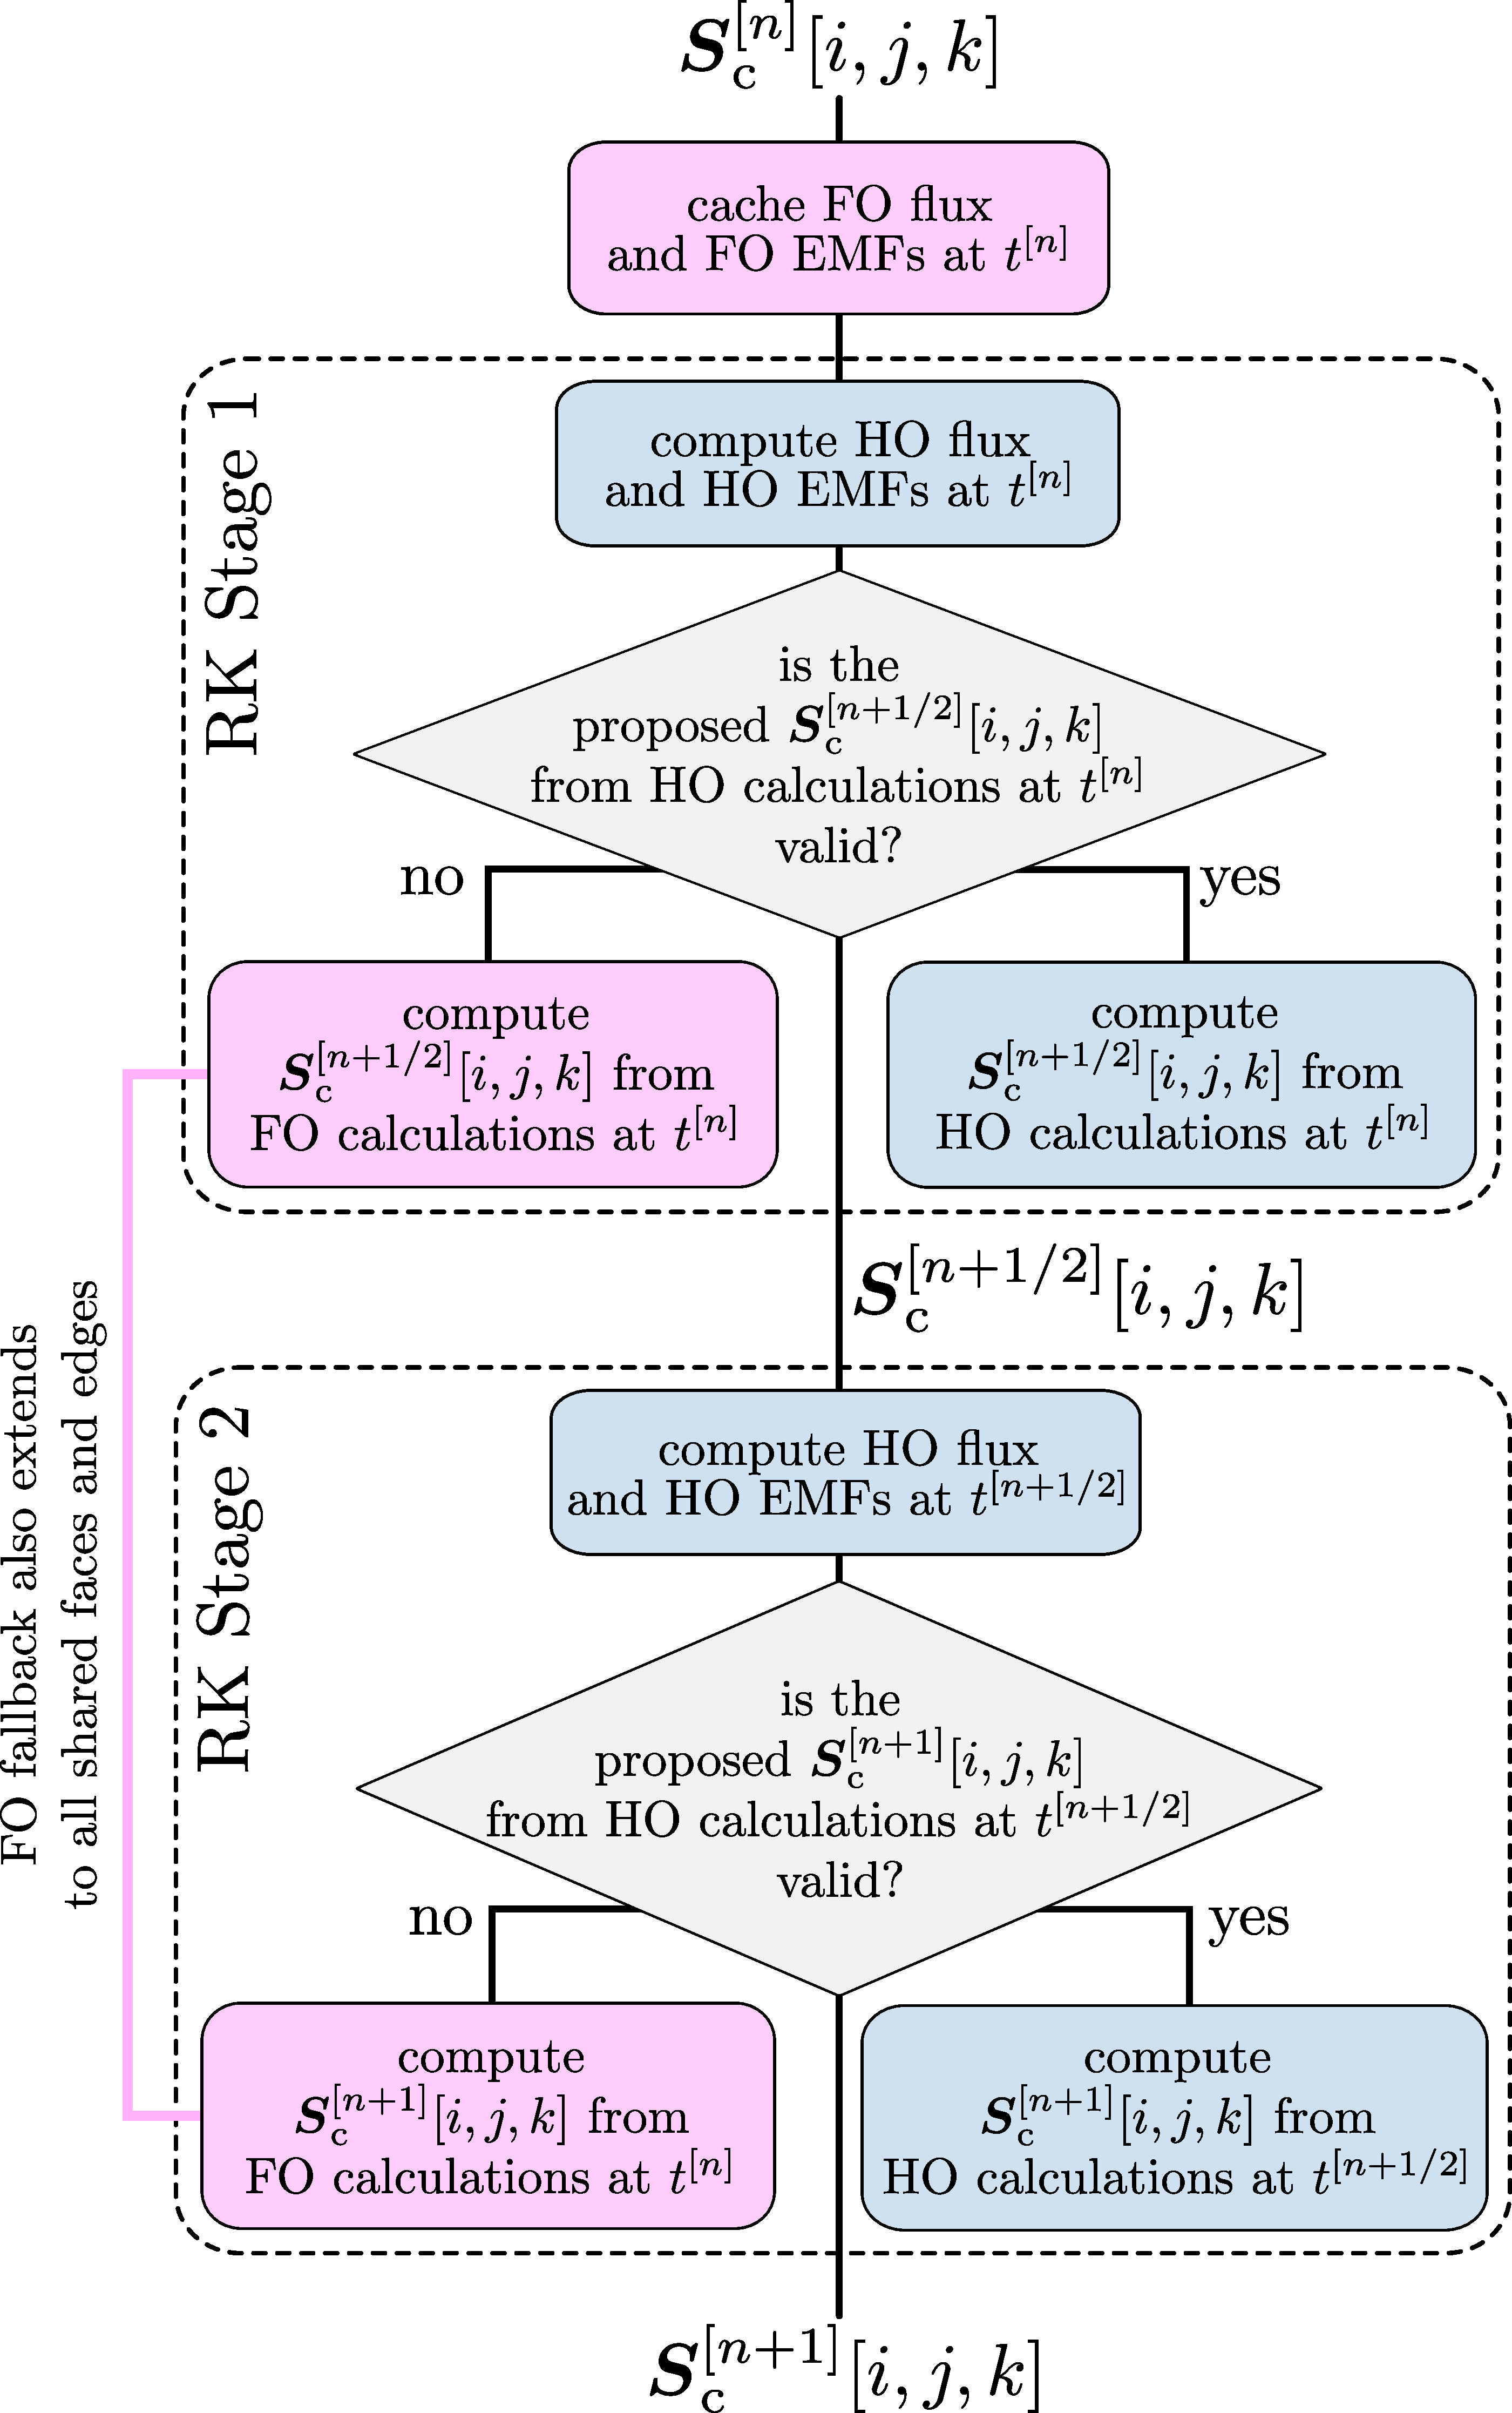
\includegraphics[width=0.65\linewidth]{figures/quokka-mhd/schematics/flowchart.pdf}
    \caption{\DIFaddFL{Flow chart of the \quokka~time stepping strategy combining RK2-SSP with first order flux correction. Here quantities labelled as high-order (HO) are computed using either PLM, PPM, or PPM-EP reconstruction and the HLLD Riemann solver, while those labelled first-order (FO) are computed using PC reconstruction and the LLF Riemann solver.}}
    \label{fig:schematic:flowchart}
\end{figure}

\begin{figure}
    \centering
    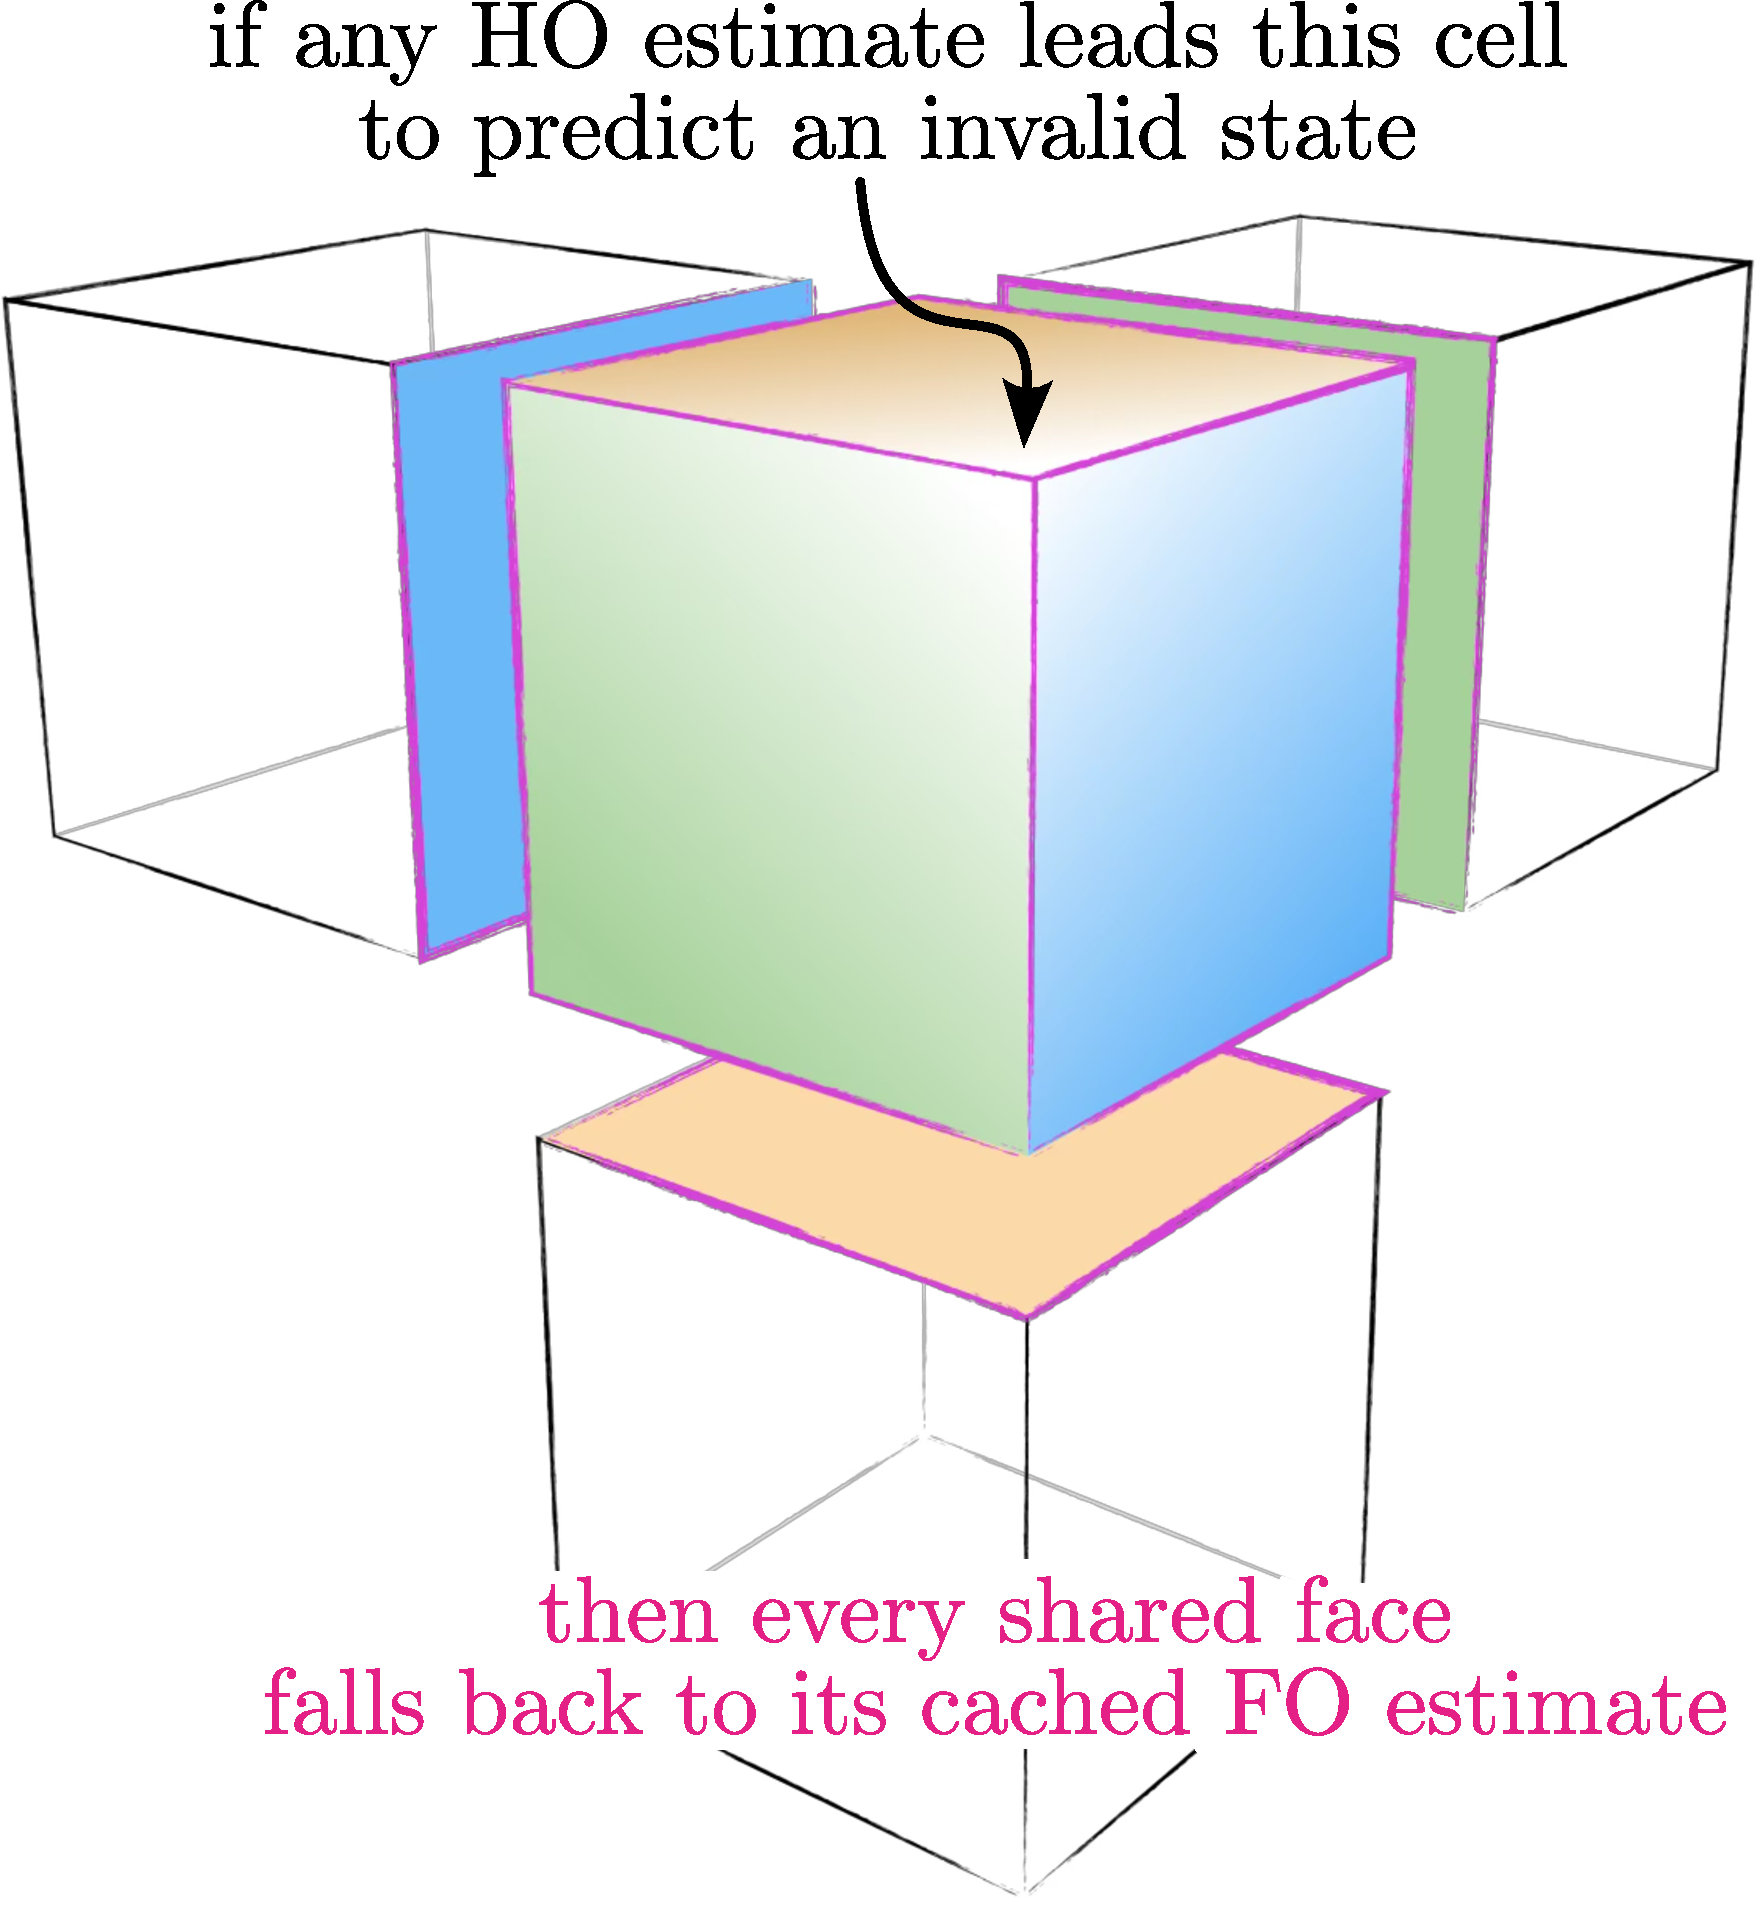
\includegraphics[width=0.5\linewidth]{figures/quokka-mhd/schematics/fofc.pdf}
    \caption{\DIFaddFL{Illustration of the first-order flux correction (FOFC) strategy. The central cell is highlighted; its shared faces with neighbouring cells fall back to cached first-order (FO) estimates if the cell's high-order (HO) update predicts an invalid state.}}
    \label{fig:fofc}
\end{figure}

\DIFadd{As }\DIFaddend in \citetalias{Wibking22a}, by default\DIFdelbegin \textsc{\DIFdel{Quokka}} %DIFAUXCMD
\DIFdel{uses }\DIFdelend \DIFaddbegin \DIFadd{, \quokka~uses a strong-stability-preserving, second-order-accurate Runge-Kutta (}\DIFaddend RK2-SSP\DIFdelbegin \footnote{\DIFdel{In problems that include the radiation submodule, we change to asymptotic-preserving IMEX PD-ARS method following \mbox{%DIFAUXCMD
\citet{Chu19a}}\hskip0pt%DIFAUXCMD
, implemented as described by \mbox{%DIFAUXCMD
\citet{He24a}}\hskip0pt%DIFAUXCMD
. However, this method reduces to RK2-SSP for the non-radiation parts of the update, including MHD, and we therefore will not bother to distinguish the two schemes here.
}} %DIFAUXCMD
\addtocounter{footnote}{-1}%DIFAUXCMD
\DIFdel{time stepping \mbox{%DIFAUXCMD
\citep{Shu88a}}\hskip0pt%DIFAUXCMD
. However, even for time steps that }\DIFdelend \DIFaddbegin \DIFadd{) time stepping strategy}\footnote{
    \DIFadd{In problems that include the radiation submodule, we change to the asymptotic-preserving IMEX PD-ARS method following \mbox{%DIFAUXCMD
\citet{Chu19a}}\hskip0pt%DIFAUXCMD
, implemented as described by \mbox{%DIFAUXCMD
\citet{He24a}}\hskip0pt%DIFAUXCMD
. However, this method reduces to RK2-SSP for the non-radiation parts of the update, including MHD, and we therefore will not distinguish the two schemes here.
}} \DIFadd{\mbox{%DIFAUXCMD
\citep{Shu88a} }\hskip0pt%DIFAUXCMD
that is robust under the standard hyperbolic CFL restriction. Even so, for strong shocks or high-Mach-number flows, this scheme can become unstable even while time steps }\DIFaddend obey the CFL condition\DIFdelbegin \DIFdel{, this method can become unstable for extreme problems}\DIFdelend ; indeed, there is no known method for guaranteeing stability in multidimensional schemes with accuracies greater than first order \DIFaddbegin \DIFadd{\mbox{%DIFAUXCMD
\citep{Godunov59a}}\hskip0pt%DIFAUXCMD
}\DIFaddend . To mitigate this problem, we introduce a modified time stepping strategy featuring a method for first order flux correction (FOFC) that maintains stability even in difficult-to-integrate flows.

\DIFdelbegin %DIFDELCMD < \begin{figure}
%DIFDELCMD <     \centering
%DIFDELCMD <     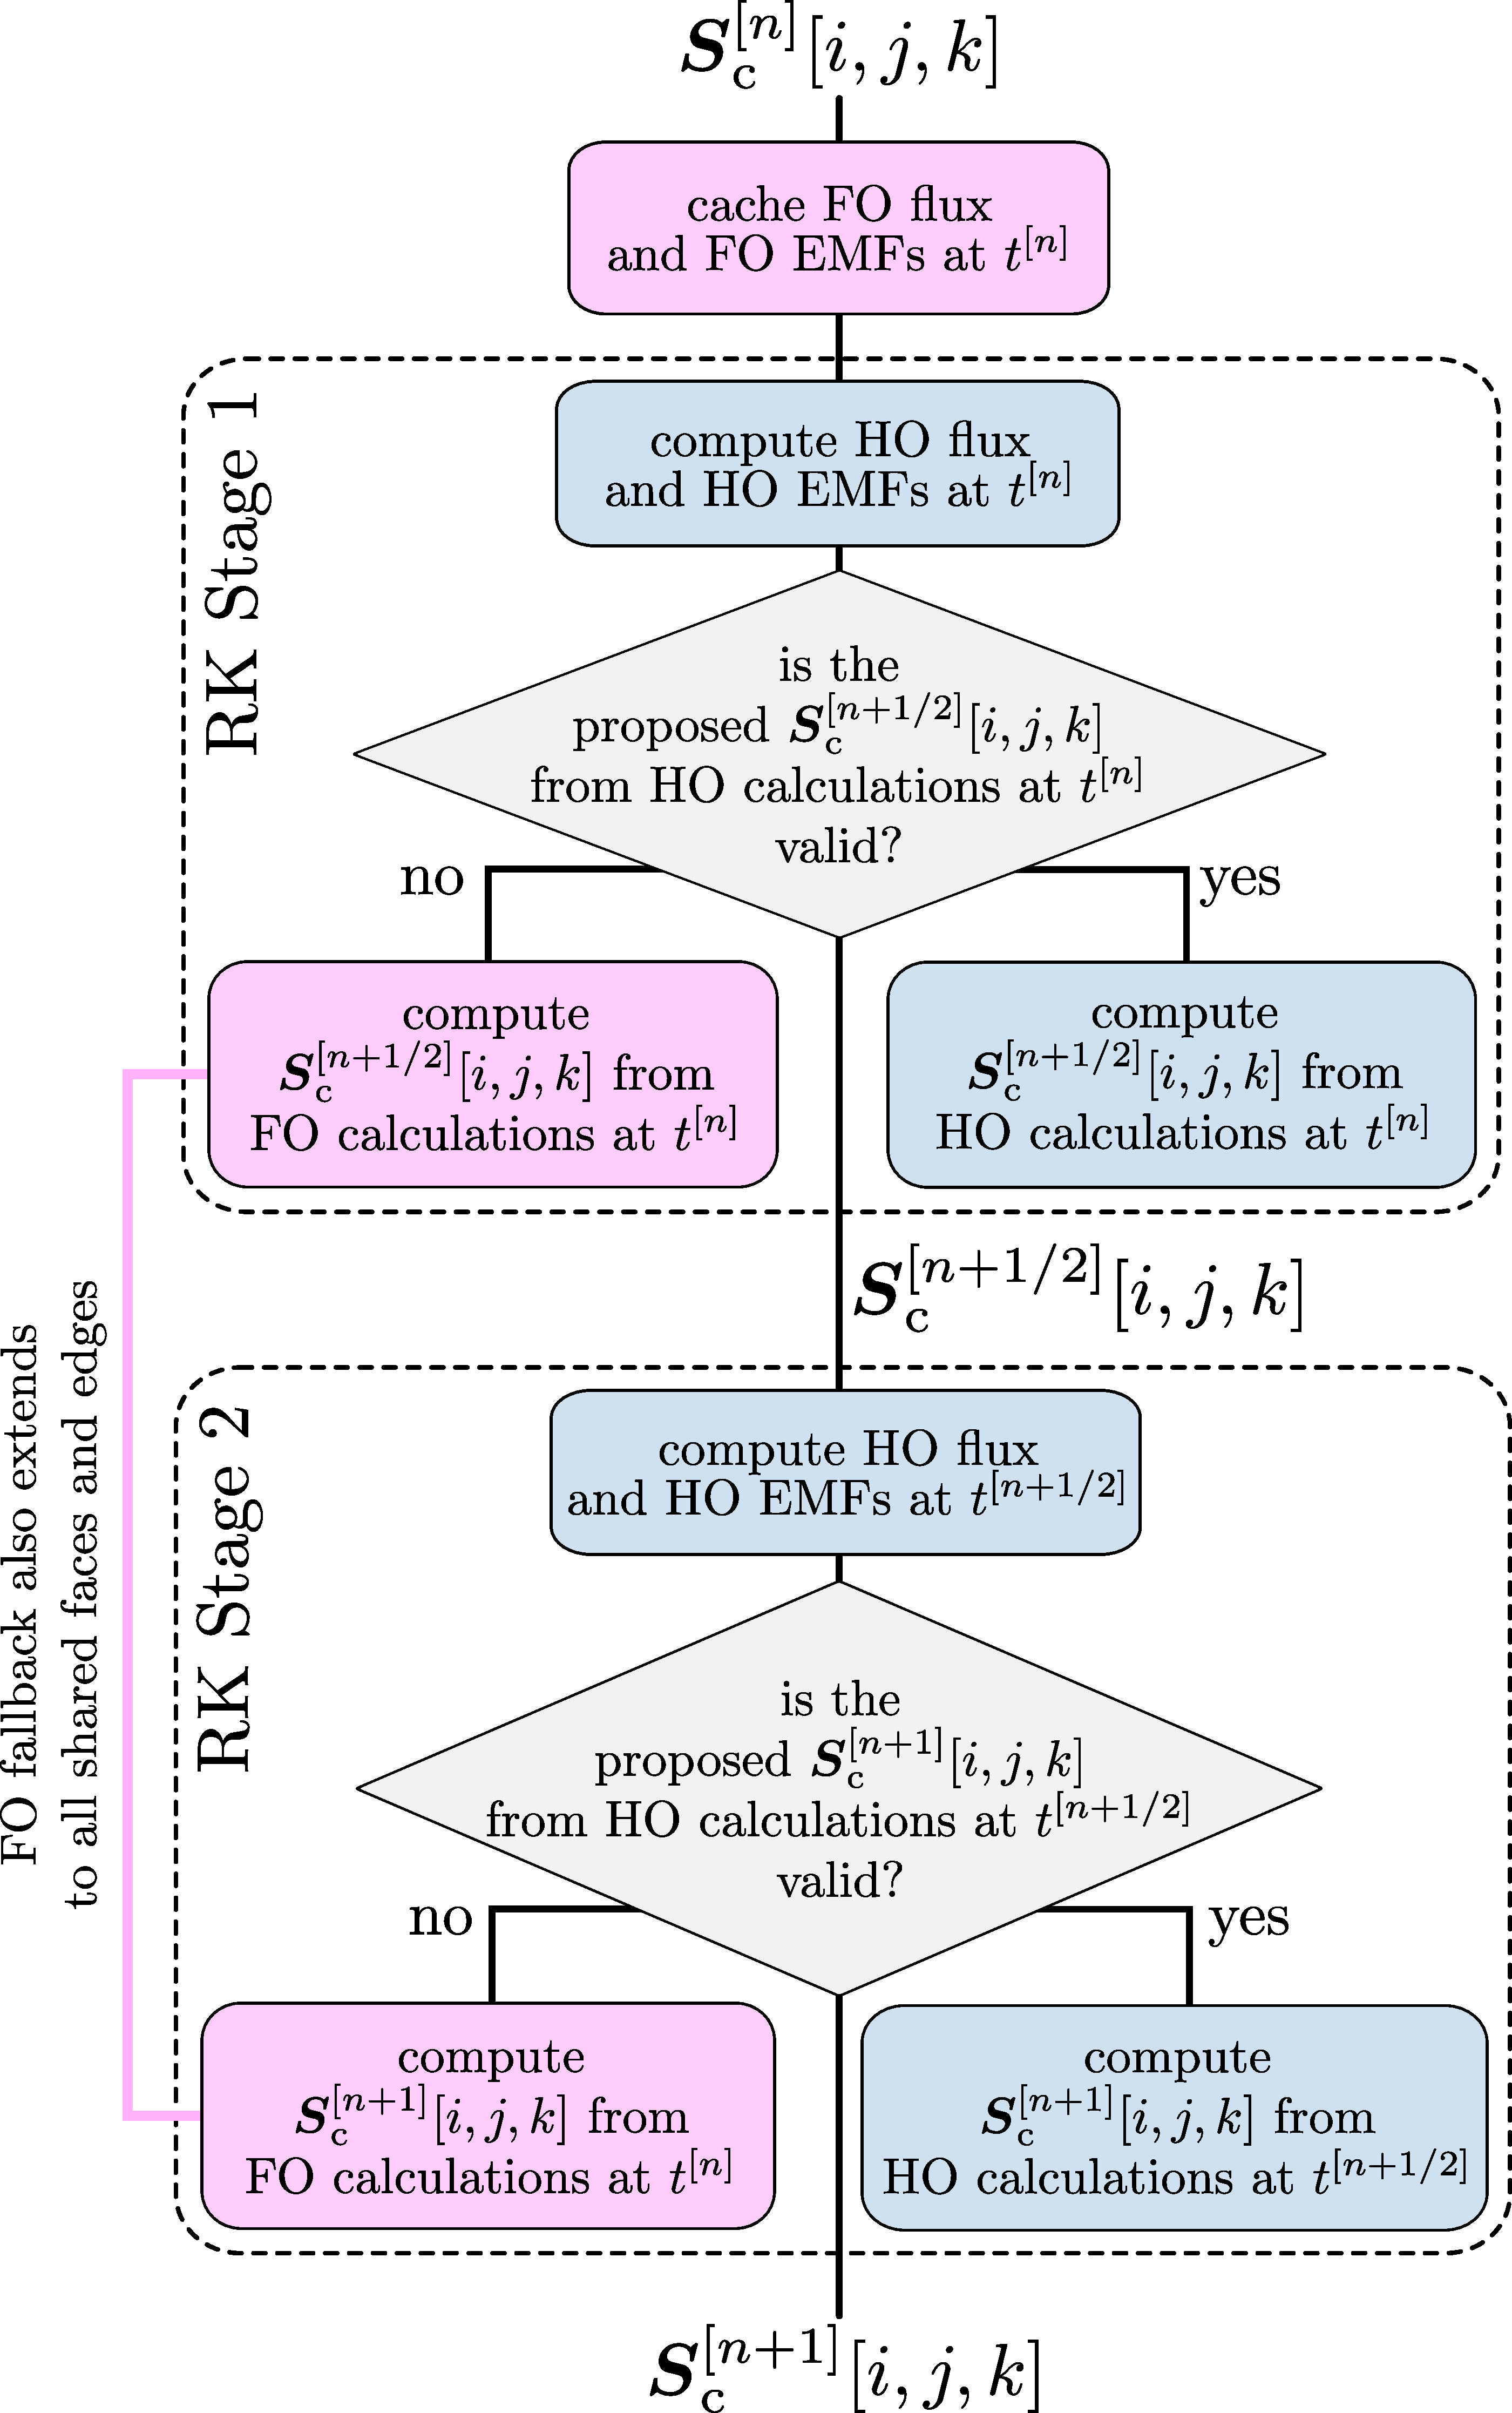
\includegraphics[width=0.7\linewidth]{figures/quokka-mhd/schematics/flowchart.pdf}
%DIFDELCMD <     %%%
%DIFDELCMD < \caption{%
{%DIFAUXCMD
\DIFdelFL{Flow chart of the }\textsc{\DIFdelFL{Quokka}} %DIFAUXCMD
\DIFdelFL{time stepping strategy combining RK2-SSP with first order flux correction. Here quantities labelled as high-order (HO) are computed using either PLM, PPM, or PPM-EP interpolation and the HLLD Riemann solver, while those labelled first-order (FO) are computed using PC interpolation and the LLF Riemann solver.}}
    %DIFAUXCMD
%DIFDELCMD < \label{fig:schematic:flowchart}
%DIFDELCMD < \end{figure}
%DIFDELCMD <

%DIFDELCMD < %%%
\DIFdel{We summarise the steps in our }\DIFdelend \DIFaddbegin \DIFadd{We describe this }\DIFaddend time stepping strategy in \DIFdelbegin %DIFDELCMD < \autoref{fig:schematic:flowchart}%%%
\DIFdel{. We start }\DIFdelend \DIFaddbegin \DIFadd{detail below, drawing attention to the different spatial stencils that the cell-centred hydrodynamic quantities and face-centred magnetic fields each depend on; the key steps of the strategy are summarised in \mbox{%DIFAUXCMD
\cref{fig:schematic:flowchart}}\hskip0pt%DIFAUXCMD
. Starting }\DIFaddend at time $t^{[n]}$ with a set of cell-centred conserved quantities $\mVector{S}_\mathrm{c}^{[n]}\EvalAtH{i}{j}{k}$ and face-centred magnetic fields \DIFdelbegin \DIFdel{$b_1^{[n]}\EvalAtH{i + 1/2}{j}{k}$, and similarly for $b_2$ and $b_3$. The steps are carry out to }\DIFdelend \DIFaddbegin \DIFadd{$b_0^{[n]}\EvalAtH{i + 1/2}{j}{k}$ (and similarly $b_1^{[n]}$ and $b_2^{[n]}$, though we will only highlight $b_0^{[n]}$ explicitly, below), we }\DIFaddend advance to time $t^{[n + 1]} = t^{[n]} + \Delta t$ \DIFdelbegin \DIFdel{are:}\DIFdelend \DIFaddbegin \DIFadd{as follows.}\DIFaddend \footnote{
    For simplicity we omit the extra steps involved if we are using \DIFdelbegin \textsc{\DIFdel{Quokka}}%DIFAUXCMD
\DIFdelend \DIFaddbegin \DIFadd{\quokka}\DIFaddend 's dual energy formalism. If dual energy is in use, we apply the dual energy correction \DIFaddbegin \DIFadd{described in \mbox{%DIFAUXCMD
\citetalias{Wibking22a} }\hskip0pt%DIFAUXCMD
}\DIFaddend following each calculation of a cell-centred state\DIFdelbegin \DIFdel{\mbox{%DIFAUXCMD
\citep{Wibking22a}}\hskip0pt%DIFAUXCMD
}\DIFdelend .
}
\DIFdelbegin %DIFDELCMD < \begin{enumerate}
%DIFDELCMD <     \item %%%
\DIFdel{First compute }\DIFdelend \DIFaddbegin

\DIFadd{At the start of each time step (see the first, pink box in \mbox{%DIFAUXCMD
\cref{fig:schematic:flowchart}}\hskip0pt%DIFAUXCMD
), we begin by computing }\DIFaddend a set of first-order, highly-dissipative fluxes of conserved cell-centred quantities and EMFs\DIFdelbegin \DIFdel{at }\DIFdelend \DIFaddbegin \DIFadd{, for }\DIFaddend each cell face and edge \DIFaddbegin \DIFadd{respectively, }\DIFaddend using the old-time state $\mVector{S}_\mathrm{c}^{[n]}\EvalAtH{i}{j}{k}$ and \DIFdelbegin \DIFdel{$b_1^{[n]}\EvalAtH{i + 1/2}{j}{k}$}\DIFdelend \DIFaddbegin \DIFadd{$b_0^{[n]}\EvalAtH{i + 1/2}{j}{k}$}\DIFaddend . We carry out \DIFdelbegin \DIFdel{the flux computation }\DIFdelend \DIFaddbegin \DIFadd{this flux calculation }\DIFaddend as described in \DIFdelbegin %DIFDELCMD < \autoref{sec:methods:flux}%%%
\DIFdelend \DIFaddbegin \DIFadd{\sref{sec:methods:flux}}\DIFaddend , using PC \DIFdelbegin \DIFdel{interpolation }\DIFdelend \DIFaddbegin \DIFadd{reconstruction }\DIFaddend and the LLF Riemann solver, and then \DIFdelbegin \DIFdel{we }\DIFdelend use the resulting wavespeeds \DIFdelbegin \DIFdel{(and for the Q26 method star states) to compute the }\DIFdelend \DIFaddbegin \DIFadd{to compute first-order }\DIFaddend EMFs as described in \DIFdelbegin %DIFDELCMD < \autoref{sec:methods:emf}%%%
\DIFdelend \DIFaddbegin \DIFadd{\sref{sec:methods:emf}}\DIFaddend . We denote the \DIFaddbegin \DIFadd{resulting }\DIFaddend first-order fluxes of conserved cell-centred quantities \DIFdelbegin \DIFdel{that result from this procedure }\DIFdelend as $\mVector{F}_\mathrm{FO}^{[n]}\EvalAtH{i \pm 1/2}{j}{k}$ and the corresponding EMFs as $\mVector{\varepsilon}_\mathrm{FO}^{[n]}\EvalAtH{i \pm 1/2}{j \pm 1/2}{k}$, and similarly for faces and edges in other directions\DIFdelbegin \DIFdel{.
    }%DIFDELCMD < \label{step:fo:cache}
%DIFDELCMD <     \item %%%
\DIFdel{First RK stage :
        }%DIFDELCMD < \begin{enumerate}
%DIFDELCMD <             \item %%%
\DIFdel{Compute }\DIFdelend \DIFaddbegin \DIFadd{; we cache these first-order estimates, to fall back on later in the update, should the high-order scheme produce an invalid state.
}

\DIFadd{For the first RK stage (see the first set of grouped steps in \mbox{%DIFAUXCMD
\cref{fig:schematic:flowchart}}\hskip0pt%DIFAUXCMD
), we compute }\DIFaddend a set of high-order, low-dissipation fluxes and EMFs as described in \DIFdelbegin %DIFDELCMD < \autoref{sec:methods:flux} %%%
\DIFdel{and }%DIFDELCMD < \autoref{sec:methods:emf}%%%
\DIFdel{. This }\DIFdelend \DIFaddbegin \DIFadd{\sref{sec:methods:flux} and \sref{sec:methods:emf}; this }\DIFaddend calculation is identical to \DIFdelbegin \DIFdel{that in }%DIFDELCMD < \autoref{step:fo:cache} %%%
\DIFdelend \DIFaddbegin \DIFadd{the one used to compute $\mVector{F}_\mathrm{FO}^{[n]}$ and $\mVector{\varepsilon}_\mathrm{FO}^{[n]}$ above, }\DIFaddend except that we use a higher-order \DIFdelbegin \DIFdel{interpolation }\DIFdelend \DIFaddbegin \DIFadd{reconstruction }\DIFaddend scheme (PLM, PPM, or PPM-EP as \DIFdelbegin \DIFdel{specified }\DIFdelend \DIFaddbegin \DIFadd{chosen }\DIFaddend by the user) and the HLLD Riemann solver\DIFaddbegin \DIFadd{, }\DIFaddend rather than PC \DIFdelbegin \DIFdel{and LLF . We }\DIFdelend \DIFaddbegin \DIFadd{reconstruction coupled with the LLF Riemann solver; we }\DIFaddend denote the resulting fluxes and EMFs as $\mVector{F}_\mathrm{HO}^{[n]}\EvalAtH{i \pm 1/2}{j}{k}$ and $\mVector{\varepsilon}_\mathrm{HO}^{[n]}\EvalAtH{i \pm 1/2}{j \pm 1/2}{k}$. \DIFdelbegin %DIFDELCMD < \label{step:rk1:ho}
%DIFDELCMD <             \item %%%
\DIFdel{Compute a proposed intermediate set of }\DIFdelend \DIFaddbegin \DIFadd{From a generic set of fluxes and EMFs at time step $[m]$, we define the update increment for the }\DIFaddend conserved cell-centred \DIFdelbegin \DIFdel{conserved quantitiesand }\DIFdelend \DIFaddbegin \DIFadd{quantities,
}\begin{align}
    D^{[m]}\sbrac{\mVector{S}_\mathrm{c}}\EvalAtV{i}{j}{k}
        &= \Delta t \Bigg(
            \, \frac{1}{\Delta{x_0}} \rbrac{
                \mVector{F}^{[m]}\EvalAtV{i - 1/2}{j}{k}
                - \mVector{F}^{[m]}\EvalAtV{i + 1/2}{j}{k}
            }
        \nonumber \\
        &\nquad[2]
            + \frac{1}{\Delta{x_1}} \rbrac{
                \mVector{F}^{[m]}\EvalAtV{i}{j - 1/2}{k}
                - \mVector{F}^{[m]}\EvalAtV{i}{j + 1/2}{k}
            }
        \nonumber \\
        &\nquad[2]
            + \frac{1}{\Delta{x_2}} \rbrac{
                \mVector{F}^{[m]}\EvalAtV{i}{j}{k - 1/2}
                - \mVector{F}^{[m]}\EvalAtV{i}{j}{k + 1/2}
            }
        \Bigg)
    , \label{eqn:rk:increment-state}
\end{align}
\DIFadd{and, analogously, the update increment for the }\DIFaddend face-centred magnetic fields \DIFdelbegin \DIFdel{as
            }%DIFDELCMD < \begin{align}
%DIFDELCMD <                 &\mVector{S}_\mathrm{c}^{[n + 1/2]}\EvalAtH{i}{j}{k}
%DIFDELCMD <                     = \mVector{S}_\mathrm{c}^{[n]}\EvalAtH{i}{j}{k}
%DIFDELCMD <                         + \frac{\Delta t}{\Delta{x_1}\, \Delta{x_2}\, \Delta{x_3}} \Bigg(
%DIFDELCMD <                     \nonumber \\
%DIFDELCMD <                     &\nquad[2] \, \Delta{x_2} \, \Delta{x_3} \rbrac{
%DIFDELCMD <                             \mVector{F}^{[n]}\EvalAtH{i - 1/2}{j}{k}
%DIFDELCMD <                             - \mVector{F}^{[n]}\EvalAtH{i + 1/2}{j}{k}
%DIFDELCMD <                         }
%DIFDELCMD <                     \nonumber \\
%DIFDELCMD <                     &\nquad[1] + \Delta{x_1} \, \Delta{x_3} \rbrac{
%DIFDELCMD <                             \mVector{F}^{[n]}\EvalAtH{i}{j - 1/2}{k}
%DIFDELCMD <                             - \mVector{F}^{[n]}\EvalAtH{i}{j + 1/2}{k}
%DIFDELCMD <                         }
%DIFDELCMD <                     \nonumber \\
%DIFDELCMD <                     &\nquad[1] + \Delta{x_1} \, \Delta{x_2} \rbrac{
%DIFDELCMD <                             \mVector{F}^{[n]}\EvalAtH{i}{j}{k - 1/2}
%DIFDELCMD <                             - \mVector{F}^{[n]}\EvalAtH{i}{j}{k + 1/2}
%DIFDELCMD <                         }
%DIFDELCMD <                     \Bigg)
%DIFDELCMD <                     \nonumber
%DIFDELCMD <             \end{align}%%%
\DIFdelend \DIFaddbegin \DIFadd{from the EMFs at the same time step
}\begin{align}
    D^{[m]}\sbrac{b_0}\EvalAtV{i + 1/2}{j}{k}
        &= \frac{\Delta t}{\Delta{x_1} \, \Delta{x_2}} \Bigg(
            \, \Delta{x_2} \, \varepsilon_2^{[m]}\EvalAtV{i + 1/2}{j - 1/2}{k}
            + \Delta{x_1} \, \varepsilon_1^{[m]}\EvalAtV{i + 1/2}{j}{k + 1/2}
        \nonumber \\
        &\nquad[5]
            - \Delta{x_2} \, \varepsilon_2^{[m]}\EvalAtV{i + 1/2}{j + 1/2}{k}
            - \Delta{x_1} \, \varepsilon_1^{[m]}\EvalAtV{i + 1/2}{j}{k - 1/2}
    \Bigg)
    , \label{eqn:rk:increment-bfield}
\end{align}\DIFaddend
\DIFdelbegin %DIFDELCMD < \begin{align}
%DIFDELCMD <                 &b_1^{[n + 1/2]}\EvalAtH{i + 1/2}{j}{k}
%DIFDELCMD <                     = b_1^{[n]}\EvalAtH{i + 1/2}{j}{k}
%DIFDELCMD <                         + \frac{\Delta t}{\Delta{x_2} \, \Delta{x_3}} \Bigg(
%DIFDELCMD <                     \nonumber \\
%DIFDELCMD <                     &\nquad[3] \, \Delta{x_3} \, \varepsilon_3^{[n]}\EvalAtH{i + 1/2}{j - 1/2}{k}
%DIFDELCMD <                         + \Delta{x_2} \, \varepsilon_2^{[n]}\EvalAtH{i + 1/2}{j}{k - 1/2}
%DIFDELCMD <                     \nonumber \\
%DIFDELCMD <                     &\nquad[2] - \Delta{x_3} \, \varepsilon_3^{[n]}\EvalAtH{i + 1/2}{j + 1/2}{k}
%DIFDELCMD <                         - \Delta{x_2} \, \varepsilon_2^{[n]}\EvalAtH{i + 1/2}{j}{k + 1/2}
%DIFDELCMD <                 \Bigg)
%DIFDELCMD <                 \nonumber
%DIFDELCMD <             \end{align}%%%
\DIFdelend \DIFaddbegin \DIFadd{with $D^{[m]}\sbrac{b_1}$ and $D^{[m]}\sbrac{b_2}$ defined analogously, by cyclic permutation of the indices. The first RK stage's proposed intermediate state then follows directly,
}\begin{align}
    \mVector{S}_\mathrm{c}^{[n + 1/2]}\EvalAtV{i}{j}{k}
        &= \mVector{S}_\mathrm{c}^{[n]}\EvalAtV{i}{j}{k}
            + D^{[n]}\sbrac{\mVector{S}_\mathrm{c}}\EvalAtV{i}{j}{k}
    ,
\end{align}\DIFaddend
\DIFdelbegin %DIFDELCMD < \begin{align}
%DIFDELCMD <                 b_2^{[n + 1/2]}\EvalAtH{i}{j + 1/2}{k}
%DIFDELCMD <                     = \cdots
%DIFDELCMD <                 . \label{eqn:rk1:update}
%DIFDELCMD <             \end{align}%%%
\DIFdelend \DIFaddbegin \DIFadd{and similarly for the face-centred magnetic fields,
}\begin{align}
    \scalebox{0.975}{$\displaystyle
        b_0^{[n + 1/2]}\EvalAtV{i + 1/2}{j}{k}
            = b_0^{[n]}\EvalAtV{i + 1/2}{j}{k}
                + D^{[n]}\sbrac{b_0}\EvalAtV{i + 1/2}{j}{k}
    $}
    . \label{eqn:rk1:update}
\end{align}\DIFaddend
\DIFdelbegin \DIFdel{using the HO versions of all fluxes and EMFs .
            }%DIFDELCMD < \item %%%
\DIFdel{Check is }\DIFdelend \DIFaddbegin

\DIFadd{We then check whether }\DIFaddend any of the intermediate states $\mVector{S}_\mathrm{c}^{[n + 1/2]}\EvalAtH{i}{j}{k}$ \DIFaddbegin \DIFadd{or magnetic quantities (}\eg \DIFadd{$b_0^{[n + 1/2]}\EvalAtH{i + 1/2}{j}{k}$) }\DIFaddend are physically invalid; at a minimum this means flagging cell centre states with negative densities, total energies, or internal energies, but we \DIFdelbegin \DIFdel{can also flag on additionaland more stringent }\DIFdelend \DIFaddbegin \DIFadd{also provide a hook for users to flag additional, more restrictive }\DIFaddend criteria, for example velocities that are unphysically large. \DIFdelbegin \DIFdel{Any additional flagging is calculation-dependent, and is left as an option for the user.
            }%DIFDELCMD < \item %%%
\DIFdelend For any cell \DIFdelbegin \DIFdel{$(i, j, k)$ that is }\DIFdelend \DIFaddbegin \DIFadd{$\EvalAtH{i}{j}{k}$ }\DIFaddend flagged as invalid \DIFdelbegin \DIFdel{, }\DIFdelend \DIFaddbegin \DIFadd{(see \mbox{%DIFAUXCMD
\cref{fig:fofc} }\hskip0pt%DIFAUXCMD
for an illustration), we }\DIFaddend replace the HO fluxes and EMFs for all of its faces and edges with their \DIFdelbegin \DIFdel{FO equivalents as computed in }%DIFDELCMD < \autoref{step:fo:cache}%%%
\DIFdel{. Then }\DIFdelend \DIFaddbegin \DIFadd{cached FO equivalents, $\mVector{F}_\mathrm{FO}^{[n]}\EvalAtH{i \pm 1/2}{j}{k}$ and $\mVector{\varepsilon}_\mathrm{FO}^{[n]}\EvalAtH{i \pm 1/2}{j \pm 1/2}{k}$, and }\DIFaddend recompute the cell-centred state and \DIFdelbegin \DIFdel{the }\DIFdelend face-centred magnetic fields for that cell by again applying \DIFdelbegin %DIFDELCMD < \autoref{eqn:rk1:update} %%%
\DIFdelend \DIFaddbegin \DIFadd{\mbox{%DIFAUXCMD
\cref{eqn:rk1:update} }\hskip0pt%DIFAUXCMD
}\DIFaddend with the replaced fluxes. \DIFdelbegin \DIFdel{This step and the next one are illustrated in }%DIFDELCMD < \autoref{fig:fofc}%%%
\DIFdel{.
            }%DIFDELCMD < \label{step:rk1:fofc}
%DIFDELCMD <             \item %%%
\DIFdel{Also }\DIFdelend \DIFaddbegin \DIFadd{We also }\DIFaddend recalculate $\mVector{S}_\mathrm{c}^{[n + 1/2]}\EvalAtH{i}{j}{k}$ and the face-centred magnetic fields for any cell \DIFdelbegin \DIFdel{that neighbours a flagged cell; this step ensures }\DIFdelend \DIFaddbegin \DIFadd{sharing a face with a flagged cell, to ensure }\DIFaddend that we use consistent fluxes and EMFs for the updates to all cells, a necessary condition for conservation and maintenance of $\nabla\cdot\mVector{b} = 0$.
\DIFdelbegin %DIFDELCMD < \end{enumerate}
%DIFDELCMD <     \item %%%
\DIFdel{Second RK stage :
    }%DIFDELCMD < \begin{enumerate}
%DIFDELCMD <         \item %%%
\DIFdel{Compute }\DIFdelend \DIFaddbegin

\DIFadd{For the second RK stage (see the second set of grouped steps in \mbox{%DIFAUXCMD
\cref{fig:schematic:flowchart}}\hskip0pt%DIFAUXCMD
), we compute }\DIFaddend a set of high-order fluxes and EMFs exactly as \DIFdelbegin \DIFdel{in }%DIFDELCMD < \autoref{step:rk1:ho}%%%
\DIFdel{, but now using }\DIFdelend \DIFaddbegin \DIFadd{we did to compute $\mVector{F}_\mathrm{HO}^{[n]}$ and $\mVector{\varepsilon}_\mathrm{HO}^{[n]}$ above, but we now use }\DIFaddend the intermediate-time states $\mVector{S}_\mathrm{c}^{[n + 1/2]}\EvalAtH{i}{j}{k}$ and \DIFdelbegin \DIFdel{$b_1^{[n + 1/2]}\EvalAtH{i + 1/2}{j}{k}$ as input}\DIFdelend \DIFaddbegin \DIFadd{$b_0^{[n + 1/2]}\EvalAtH{i + 1/2}{j}{k}$ as inputs}\DIFaddend . We denote these fluxes and EMFs as $\mVector{F}_\mathrm{HO}^{[n + 1/2]}\EvalAtH{i \pm 1/2}{j}{k}$ and $\mVector{\varepsilon}_\mathrm{HO}^{[n + 1/2]}\EvalAtH{i \pm 1/2}{j \pm 1/2}{k}$\DIFdelbegin \DIFdel{.
        }%DIFDELCMD < \item %%%
\DIFdel{Compute a proposed final set of conserved cell-centred conserved quantities and face-centred magnetic fields as
            }%DIFDELCMD < \begin{align}
%DIFDELCMD <                 \mVector{S}_\mathrm{c}^{[n + 1]}\EvalAtH{i}{j}{k}
%DIFDELCMD <                     &= \mVector{S}_\mathrm{c}^{[n]}\EvalAtH{i}{j}{k}
%DIFDELCMD <                         + \frac{\Delta t}{2 \Delta{x_1}\, \Delta{x_2}\, \Delta{x_3}} \Bigg(
%DIFDELCMD <                     \nonumber \\
%DIFDELCMD <                     &\nquad[2] \, \Delta{x_2} \, \Delta{x_3} \left(
%DIFDELCMD <                                 \mVector{F}^{[n]}\EvalAtH{i - 1/2}{j}{k}
%DIFDELCMD <                                 - \mVector{F}^{[n]}\EvalAtH{i + 1/2}{j}{k}
%DIFDELCMD <                             \right)
%DIFDELCMD <                     \nonumber \\
%DIFDELCMD <                     &\nquad[1] + \Delta{x_1} \, \Delta{x_3} \rbrac{
%DIFDELCMD <                                 \mVector{F}^{[n]}\EvalAtH{i}{j - 1/2}{k}
%DIFDELCMD <                                 - \mVector{F}^{[n]}\EvalAtH{i}{j + 1/2}{k}
%DIFDELCMD <                             }
%DIFDELCMD <                     \nonumber \\
%DIFDELCMD <                     &\nquad[1] + \Delta{x_1} \, \Delta{x_2} \rbrac{
%DIFDELCMD <                                 \mVector{F}^{[n]}\EvalAtH{i}{j}{k - 1/2}
%DIFDELCMD <                                 - \mVector{F}^{[n]}\EvalAtH{i}{j}{k + 1/2}
%DIFDELCMD <                             }
%DIFDELCMD <                     \nonumber \\
%DIFDELCMD <                     &\nquad[1] + \Delta{x_2} \, \Delta{x_3} \rbrac{
%DIFDELCMD <                                 \mVector{F}^{[n + 1/2]}\EvalAtH{i - 1/2}{j}{k}
%DIFDELCMD <                                 - \mVector{F}^{[n + 1/2]}\EvalAtH{i + 1/2}{j}{k}
%DIFDELCMD <                             }
%DIFDELCMD <                     \nonumber \\
%DIFDELCMD <                     &\nquad[1] + \Delta{x_1} \, \Delta{x_3} \rbrac{
%DIFDELCMD <                                 \mVector{F}^{[n + 1/2]}\EvalAtH{i}{j - 1/2}{k}
%DIFDELCMD <                                 - \mVector{F}^{[n + 1/2]}\EvalAtH{i}{j + 1/2}{k}
%DIFDELCMD <                             }
%DIFDELCMD <                     \nonumber \\
%DIFDELCMD <                     &\nquad[1] + \Delta{x_1} \, \Delta{x_2} \rbrac{
%DIFDELCMD <                                 \mVector{F}^{[n + 1/2]}\EvalAtH{i}{j}{k - 1/2}
%DIFDELCMD <                                 - \mVector{F}^{[n + 1/2]}\EvalAtH{i}{j}{k + 1/2}
%DIFDELCMD <                             }
%DIFDELCMD <                 \Bigg)
%DIFDELCMD <                 \nonumber
%DIFDELCMD <             \end{align}
%DIFDELCMD <             \begin{align}
%DIFDELCMD <                 &b_1^{[n + 1]}\EvalAtH{i + 1/2}{j}{k}
%DIFDELCMD <                     = b_1^{[n]}\EvalAtH{i + 1/2}{j}{k}
%DIFDELCMD <                         + \frac{\Delta t}{2 \Delta{x_2} \, \Delta{x_3}} \Bigg(
%DIFDELCMD <                     \nonumber \\
%DIFDELCMD <                     &\nquad[2] \, \Delta{x_3} \, \varepsilon_3^{[n]}\EvalAtH{i + 1/2}{j - 1/2}{k}
%DIFDELCMD <                         + \Delta{x_2} \, \varepsilon_2^{[n]}\EvalAtH{i + 1/2}{j}{k - 1/2}
%DIFDELCMD <                     \nonumber \\
%DIFDELCMD <                     &\nquad[1] - \Delta{x_3} \, \varepsilon_3^{[n]}\EvalAtH{i + 1/2}{j + 1/2}{k}
%DIFDELCMD <                         - \Delta{x_2} \, \varepsilon_2^{[n]}\EvalAtH{i + 1/2}{j}{k + 1/2}
%DIFDELCMD <                     \nonumber \\
%DIFDELCMD <                     &\nquad[1] + \Delta{x_3} \, \varepsilon_3^{[n + 1/2]}\EvalAtH{i + 1/2}{j - 1/2}{k}
%DIFDELCMD <                         + \Delta{x_2} \, \varepsilon_2^{[n + 1/2]}\EvalAtH{i + 1/2}{j}{k - 1/2}
%DIFDELCMD <                     \nonumber \\
%DIFDELCMD <                     &\nquad[1] - \Delta{x_3} \, \varepsilon_3^{[n + 1/2]}\EvalAtH{i + 1/2}{j + 1/2}{k}
%DIFDELCMD <                         - \Delta{x_2} \, \varepsilon_2^{[n + 1/2]}\EvalAtH{i + 1/2}{j}{k + 1/2}
%DIFDELCMD <                 \Bigg)
%DIFDELCMD <                 \nonumber
%DIFDELCMD <             \end{align}
%DIFDELCMD <             \begin{align}
%DIFDELCMD <                 b_2^{[n + 1]}\EvalAtH{i}{j + 1/2}{k}
%DIFDELCMD <                     = \cdots
%DIFDELCMD <                 . \label{eqn:rk2:update}
%DIFDELCMD <             \end{align}
%DIFDELCMD <         %%%
\DIFdel{In this calculation we use the fluxes and EMFs at time }\DIFdelend \DIFaddbegin \DIFadd{, giving access to the update increments $D^{[n + 1/2]}\sbrac{\mVector{S}_\mathrm{c}}$ and $D^{[n + 1/2]}\sbrac{b_0}$ following \mbox{%DIFAUXCMD
\cref{eqn:rk:increment-state,eqn:rk:increment-bfield}}\hskip0pt%DIFAUXCMD
. Together with the increments at time step }\DIFaddend $[n]$\DIFaddbegin \DIFadd{, }\DIFaddend determined during the first RK stage (\DIFdelbegin \DIFdel{HO }\DIFdelend \DIFaddbegin \DIFadd{using the HO fluxes and EMFs, }\DIFaddend unless they were replaced \DIFdelbegin \DIFdel{during }%DIFDELCMD < \autoref{step:rk1:fofc}%%%
\DIFdel{), and we use the HO fluxes at time $[n + 1/2]$.
        }%DIFDELCMD < \item %%%
\DIFdel{Again }\DIFdelend \DIFaddbegin \DIFadd{by their cached FO equivalents), the second RK stage's proposed final state is simply the average of both time steps' increments,
}\begin{align}
    \mVector{S}_\mathrm{c}^{[n + 1]}\EvalAtV{i}{j}{k}
        = \mVector{S}_\mathrm{c}^{[n]}\EvalAtV{i}{j}{k}
            &+ \frac{1}{2}\Bigg(
            D^{[n]}\sbrac{\mVector{S}_\mathrm{c}}\EvalAtV{i}{j}{k}
            + D^{[n + 1/2]}\sbrac{\mVector{S}_\mathrm{c}}\EvalAtV{i}{j}{k}
        \Bigg)
    ,
\end{align}
\DIFadd{and similarly for the face-centred magnetic fields,
}\begin{align}
    \scalebox{0.925}{$\displaystyle
    b_0^{[n + 1]}\EvalAtV{i + 1/2}{j}{k}
        = b_0^{[n]}\EvalAtV{i + 1/2}{j}{k}
            + \frac{1}{2}\Bigg(
            D^{[n]}\sbrac{b_0}\EvalAtV{i + 1/2}{j}{k}
            + D^{[n + 1/2]}\sbrac{b_0}\EvalAtV{i + 1/2}{j}{k}
        \Bigg)
    $}, \label{eqn:rk2:update}
\end{align}

\DIFadd{We again }\DIFaddend check for physically invalid states $\mVector{S}_\mathrm{c}^{[n + 1]}\EvalAtH{i}{j}{k}$ in any cells\DIFdelbegin \DIFdel{. If }\DIFdelend \DIFaddbegin \DIFadd{; if }\DIFaddend an invalid state is found, \DIFdelbegin \DIFdel{replace the intermediate-time, $[n + 1/2]$, }\DIFdelend \DIFaddbegin \DIFadd{we replace the RK-averaged }\DIFaddend fluxes and EMFs on that cell's faces and edges \DIFdelbegin \DIFdel{with the FO ones determined during }%DIFDELCMD < \autoref{step:fo:cache}%%%
\DIFdel{, and }\DIFdelend \DIFaddbegin \DIFadd{(\mbox{%DIFAUXCMD
\cref{eqn:rk2:update}}\hskip0pt%DIFAUXCMD
) outright with their cached FO equivalents, $\mVector{F}_\mathrm{FO}^{[n]}\EvalAtH{i \pm 1/2}{j}{k}$ and $\mVector{\varepsilon}_\mathrm{FO}^{[n]}\EvalAtH{i \pm 1/2}{j \pm 1/2}{k}$, which reduces that cell's full time step to a first-order, forwards Euler update regardless of whether its first RK stage used HO or FO fluxes. We then }\DIFaddend recompute $\mVector{S}_\mathrm{c}^{[n + 1]}\EvalAtH{i}{j}{k}$ and \DIFdelbegin \DIFdel{$b_1^{[n + 1]}\EvalAtH{i + 1/2}{j}{k}$ }\DIFdelend \DIFaddbegin \DIFadd{$b_0^{[n + 1]}\EvalAtH{i + 1/2}{j}{k}$ }\DIFaddend in both the flagged cell and \DIFdelbegin \DIFdel{all its neighbours }\DIFdelend \DIFaddbegin \DIFadd{every cell sharing a face with it, }\DIFaddend using the replaced fluxes.
\DIFdelbegin %DIFDELCMD < \end{enumerate}
%DIFDELCMD < \end{enumerate}
%DIFDELCMD < %%%
\DIFdelend

\DIFdelbegin %DIFDELCMD < \begin{figure}
%DIFDELCMD <     \centering
%DIFDELCMD <     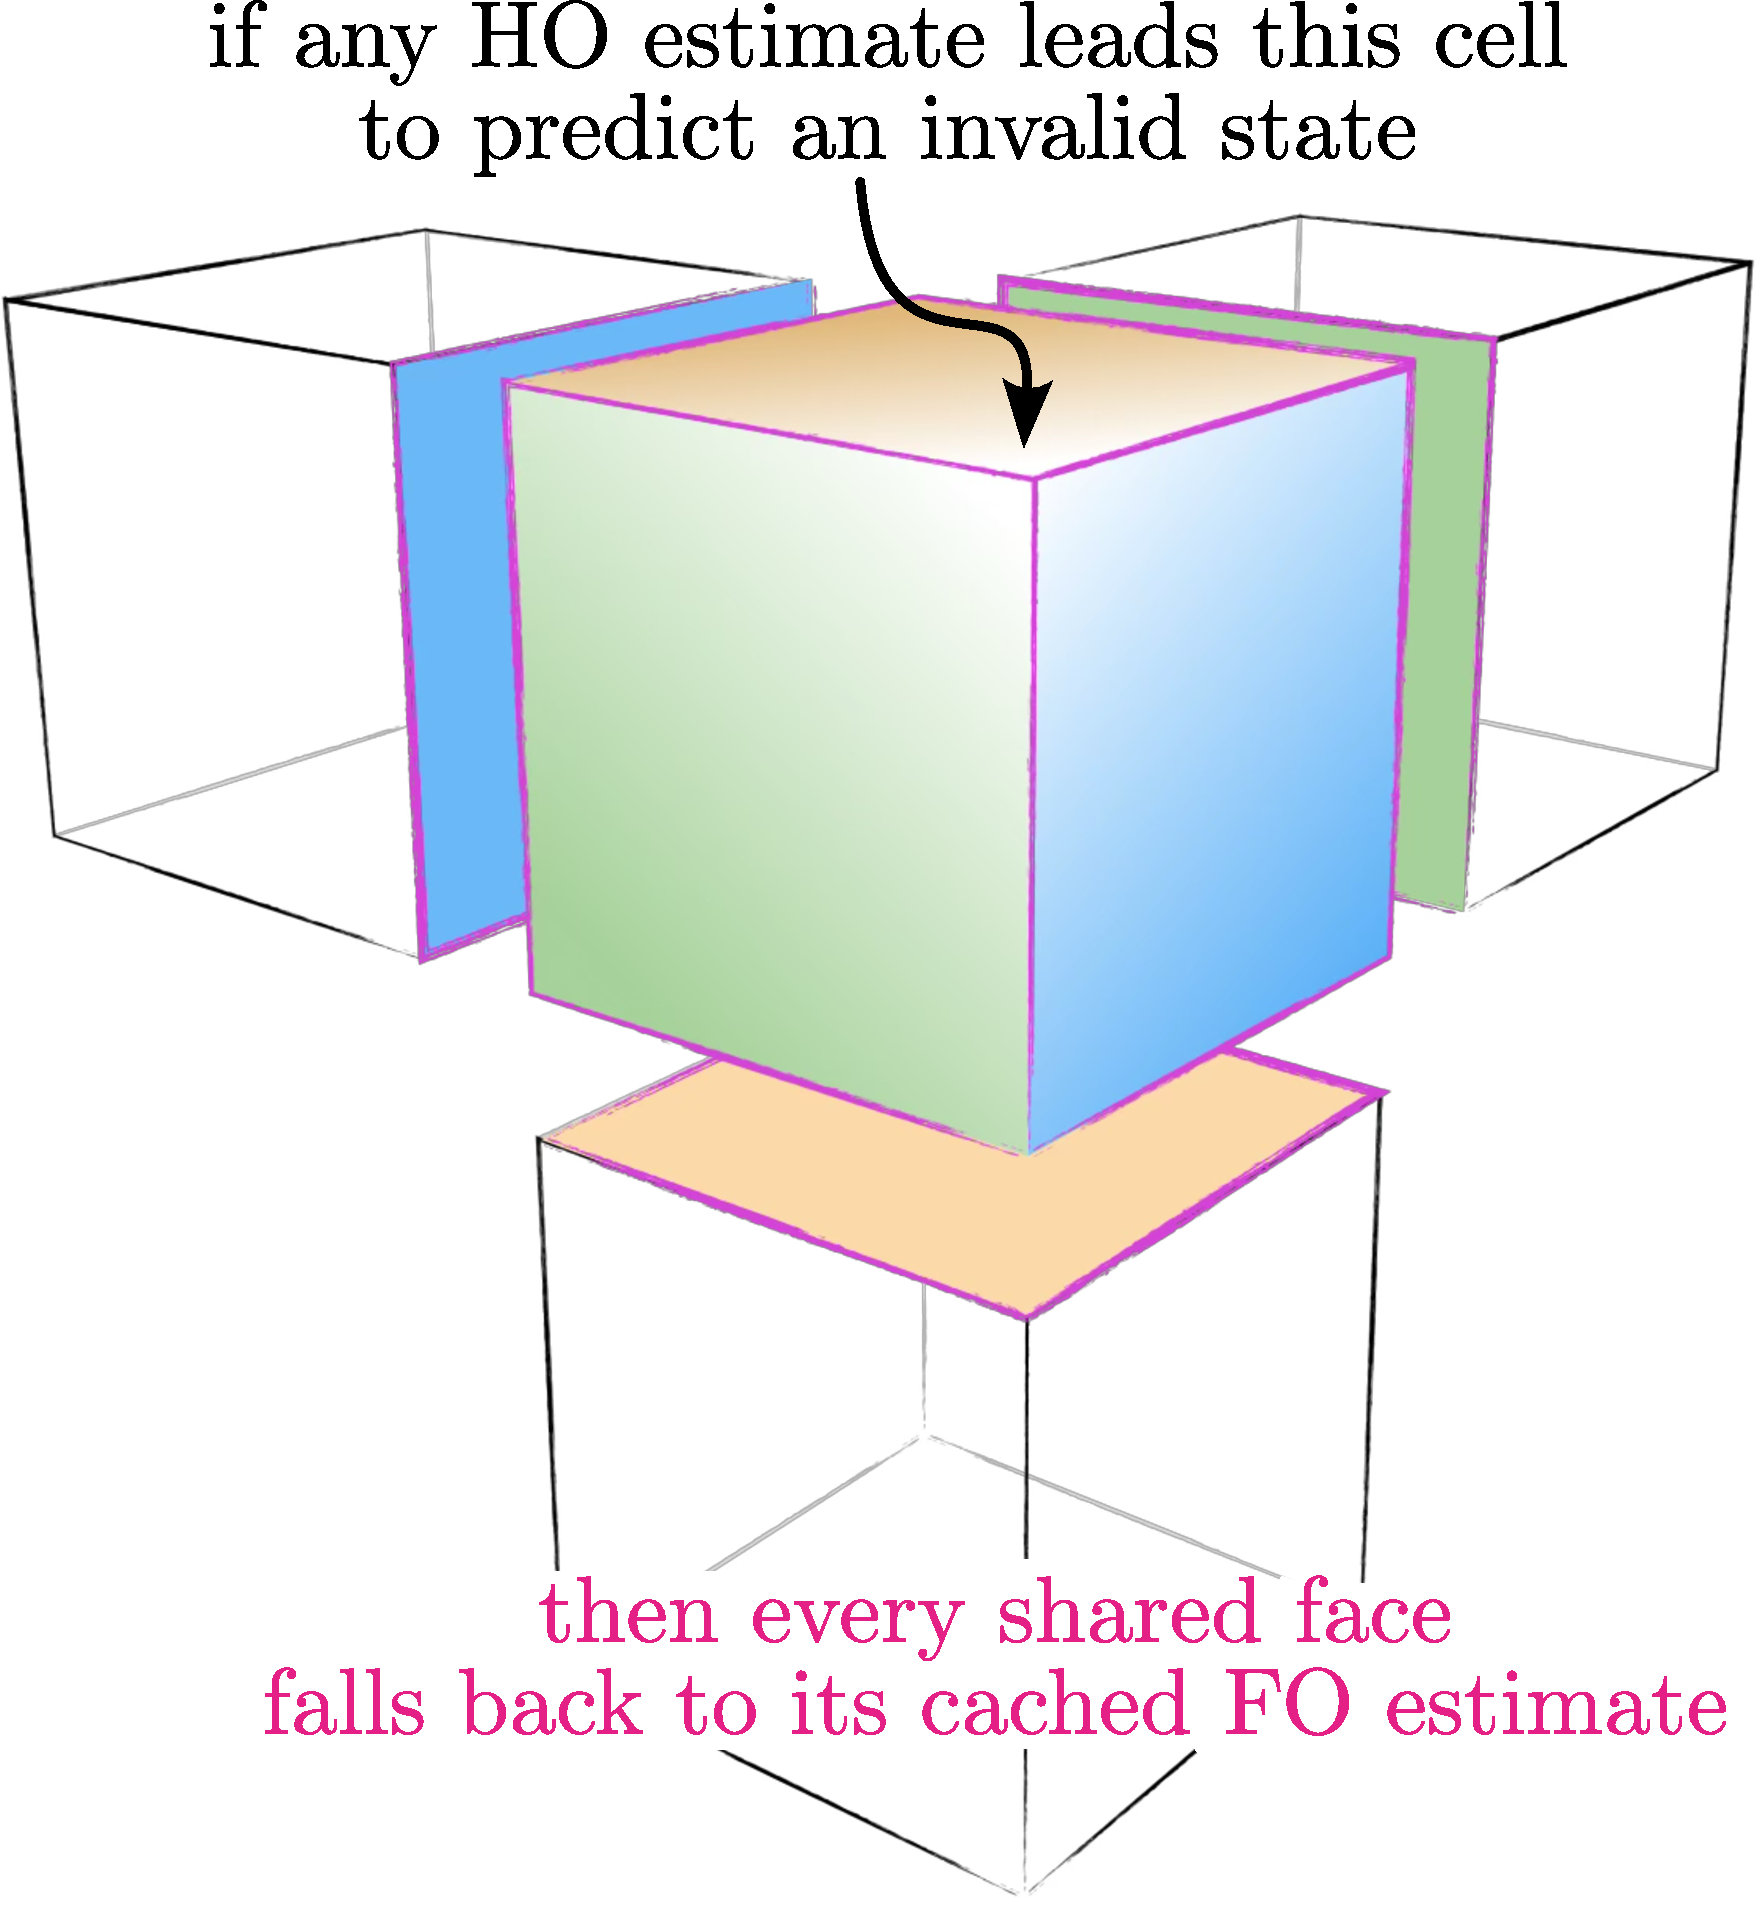
\includegraphics[width=0.55\linewidth]{figures/quokka-mhd/schematics/fofc.pdf}
%DIFDELCMD <     %%%
%DIFDELCMD < \caption{%
{%DIFAUXCMD
\DIFdelFL{Illustration of the first-order flux correction (FOFC) scheme. If the predicted cell-centred state of a cell computed using a high-order method (HO) is flagged as invalid after either the first or second RK stage, the fluxes on each of its faces and the EMFs on each of its edges are replaced by first-order (FO) estimates, and the update is recomputed both the flagged cell, for all of its neighbours that share a face or edge whose flux or EMF has been replaced.}}
    %DIFAUXCMD
%DIFDELCMD < \label{fig:fofc}
%DIFDELCMD < \end{figure}
%DIFDELCMD <

%DIFDELCMD < %%%
\DIFdelend This completes the update cycle. Note that if no flux replacements take place in either of the RK stages, then this update reduces to a standard RK2-SSP \DIFdelbegin \DIFdel{method}\DIFdelend \DIFaddbegin \DIFadd{scheme}\DIFaddend . Conversely, if \DIFdelbegin \DIFdel{we replace }\DIFdelend the HO fluxes \DIFaddbegin \DIFadd{are replaced }\DIFaddend with FO fluxes during both RK stages, \DIFdelbegin \DIFdel{this update procedure }\DIFdelend \DIFaddbegin \DIFadd{the update across the full time step }\DIFaddend reduces to a \DIFdelbegin \DIFdel{simple }\DIFdelend first order in time\DIFaddbegin \DIFadd{, }\DIFaddend forwards Euler update\DIFdelbegin \DIFdel{, with the fluxes and EMFs in turn determined from a first order in space interpolation procedure. Thus the entire scheme consistently falls back to first order if itencounters a bad state, hence our description of the scheme as FOFC . However, our procedure }\DIFdelend \DIFaddbegin \DIFadd{. Importantly, this update only affects the cells that require it, so regions that are well behaved still achieve a higher-order update. Moreover, the benefit of this FOFC strategy is that it }\DIFaddend can also yield an intermediate \DIFdelbegin \DIFdel{approximation if the HO flux is replaced by a FO flux at one but not both of the RK stages. In this case we obtain an estimate that is intermediate in terms of accuracy}\DIFdelend \DIFaddbegin \DIFadd{level of approximation, between a full FO and a full HO update, when only the first RK stage requires correction, since the second stage's HO fluxes still contribute their half-weight to the final update; a cell that instead requires correction at the second stage reverts fully to a first-order update for that step, irrespective of whether its first stage used HO or FO fluxes}\DIFaddend .

%DIF <  Borris correction: MHD eqns make the assumption that
\DIFdelbegin %DIFDELCMD <

%DIFDELCMD < %%%
\DIFdelend \subsection{AMR considerations}
\label{sec:methods:amr}

\DIFdelbegin \DIFdel{The scheme we have just described is naturally extensible to AMR. }\textsc{\DIFdel{Quokka}} %DIFAUXCMD
\DIFdelend \DIFaddbegin \DIFadd{\quokka~}\DIFaddend uses \citet{Berger84a} block-structured AMR with \citet{Berger89a} adaptive time stepping\DIFaddbegin \DIFadd{, }\DIFaddend as implemented in the \textsc{AMReX} library \citep{Zhang19b}\DIFdelbegin \DIFdel{, }\DIFdelend \DIFaddbegin \DIFadd{. Because the cell-centred part of our scheme (reconstruction, the Riemann solve, and the FOFC fallback) is applied entirely locally, on a per-cell }\DIFaddend and \DIFdelbegin \DIFdel{applying this approach to our MHD scheme }\DIFdelend \DIFaddbegin \DIFadd{per-level basis, it extends to AMR exactly as it does for pure hydrodynamics in \mbox{%DIFAUXCMD
\citetalias{Wibking22a}}\hskip0pt%DIFAUXCMD
, and also naturally accommodates adaptive, subcycled time stepping across refinement levels; coarse-fine consistency for the cell-centred quantities is enforced by \quokka's existing flux-register machinery. Supporting the face-centred magnetic field under AMR, however, }\DIFaddend requires two additional ingredients \DIFaddbegin \DIFadd{specific to CT}\DIFaddend : a method to refine or coarsen the face-centred \DIFdelbegin \DIFdel{magnetic field quantities when increasing or decreasing the resolution }\DIFdelend \DIFaddbegin \DIFadd{field when the resolution changes}\DIFaddend , and a method to correct for \DIFdelbegin \DIFdel{mismatches in the flux }\DIFdelend \DIFaddbegin \DIFadd{EMF-driven flux mismatches }\DIFaddend across coarse-fine \DIFdelbegin \DIFdel{level }\DIFdelend boundaries. For refinement and coarsening, \DIFdelbegin \textsc{\DIFdel{Quokka}} %DIFAUXCMD
\DIFdelend \DIFaddbegin \DIFadd{\quokka~}\DIFaddend uses the divergence-preserving interpolator introduced by \citet{Vanella10a}, and implemented as part of \textsc{AMReX}. This guarantees that the discrete magnetic divergence remains zero when we add or remove levels, or when we fill ghost zones. For flux mismatches, we implement the flux-correction scheme described by \citet{Balsara01a}, and also used in the \textsc{orion2} code \citep{Li12a}. Briefly, this scheme corrects the magnetic field estimate on coarse cell faces that lie at coarse-fine boundaries to ensure that they are updated using the same EMFs as were used to update the fine cell faces, thereby maintaining zero divergence across coarse-fine interfaces.


\section{Comparison of Schemes}
\DIFdelbegin %DIFDELCMD < \label{sec:performance}
%DIFDELCMD < %%%
\DIFdelend \DIFaddbegin \label{sec:scheme-comparisons}
\DIFaddend

\DIFdelbegin %DIFDELCMD < \autoref{sec:methods:emf} %%%
\DIFdel{introduces three }\DIFdelend \DIFaddbegin \DIFadd{\sref{sec:methods:emf} introduced three EMF compute schemes and two EMF averaging }\DIFaddend schemes\DIFdelbegin \DIFdel{for extrapolating EMFs to cell edges and two for averaging them together}\DIFdelend , each of which can \DIFdelbegin \DIFdel{be combined with PC, }\DIFdelend \DIFaddbegin \DIFadd{independently be paired with }\DIFaddend PLM, PPM, \DIFdelbegin \DIFdel{and }\DIFdelend \DIFaddbegin \DIFadd{or }\DIFaddend PPM-EP \DIFdelbegin \DIFdel{interpolation. Our next goal is to compare the performance of these schemes.
}\DIFdelend \DIFaddbegin \DIFadd{reconstruction, giving 18 distinct scheme combinations in total. Our main interest is how the choice of EMF compute and averaging scheme affects numerical dissipation, and how the total number of compute steps in each scheme combination affects performance. We therefore systematically validate all 18 combinations against a range of test problems}\footnote{
    \DIFadd{\quokka~is a 3D code, so 1D and 2D test problems are set up to repeat along the remaining trivial axes. We give each of these axes the minimum number of cells needed for ghost-zone exchange. For all test problems, we therefore only state resolutions along the axes where the solution actually varies.
    }\label{note:quokka:3d}
}\DIFadd{, before comparing them directly against one another.
}

\DIFaddend To this end, we first test \DIFdelbegin \DIFdel{their convergence in simulating linear }\DIFdelend \DIFaddbegin \DIFadd{the numerical convergence of each scheme in our suite against }\DIFaddend MHD waves in \DIFdelbegin %DIFDELCMD < \autoref{sec:performance:waves} %%%
\DIFdel{and their }\DIFdelend \DIFaddbegin \DIFadd{\sref{sec:scheme-comparison:waves}, isolating the accuracy of the reconstruction scheme in smooth flow regimes; we then test each scheme's }\DIFaddend ability to capture \DIFdelbegin \DIFdel{magnetised shocks in }%DIFDELCMD < \autoref{sec:performance:brio-wu}%%%
\DIFdel{, followed by }%DIFDELCMD < \autoref{sec:performance:orszag-tang} %%%
\DIFdel{where we test their stability and accuracy in a challengingmultidimensional, }\DIFdelend \DIFaddbegin \DIFadd{and resolve shocks in \sref{sec:scheme-comparison:shocks}, where discontinuities stress the Riemann solver; and finally, we test the full suite against two more challenging, multidimensional }\DIFaddend non-linear \DIFdelbegin \DIFdel{problem. We then evaluate their relative speed in }%DIFDELCMD < \autoref{sec:performance:speed}%%%
\DIFdel{, before making final recommendations in }%DIFDELCMD < \autoref{sec:performance:summary}%%%
\DIFdel{. Unless noted otherwise, all the tests reported in this section and the next one were carried out on the Setonix machine at the Pawsey Supercomputing Centre in Western Australia.
Each node of this machine provides four AMD Instinct MI-250X GPU cards with two logical GPUs per card; nodes are linked with HPE Slingshot interconnects.
}\DIFdelend \DIFaddbegin \DIFadd{problems in \sref{sec:scheme-comparison:orszag-tang} and \sref{sec:scheme-comparison:reconnection}. These problems exercise all aspects of the solver. We then measure the relative performance throughput of each scheme in \sref{sec:scheme-comparison:speed}, before recommending in \sref{sec:scheme-comparison:recommendation} which scheme to use in \quokka.
}\DIFaddend

\subsection{Convergence \DIFdelbegin \DIFdel{for linear }\DIFdelend \DIFaddbegin \DIFadd{of magnetosonic }\DIFaddend waves}
\DIFdelbegin %DIFDELCMD < \label{sec:performance:waves}
%DIFDELCMD < %%%
\DIFdelend \DIFaddbegin \label{sec:scheme-comparison:waves}
\DIFaddend

\DIFdelbegin \DIFdel{We first test the basic accuracy and convergence of our schemes for two simple linear waves: a linearly-polarised }\DIFdelend \DIFaddbegin \DIFadd{For all four waves in the MHD family (linearly and circularly-polarised }\DIFaddend Alfv\'en \DIFdelbegin \DIFdel{wave and a fast wave. For both waves, we consider }\DIFdelend \DIFaddbegin \DIFadd{waves, the fast magnetosonic wave, and the slow magnetosonic wave), we start by considering }\DIFaddend a uniform background state
\DIFdelbegin %DIFDELCMD < \begin{align}
%DIFDELCMD <     \mVector{S}_\mathrm{c}^{\{0\}}
%DIFDELCMD <         = \begin{Bmatrix}
%DIFDELCMD <                 \rho \\
%DIFDELCMD <                 \rho \mVector{u} \\
%DIFDELCMD <                 e_\mathrm{tot} \\
%DIFDELCMD <                 \mVector{b}
%DIFDELCMD <             \end{Bmatrix}
%DIFDELCMD <         = \begin{Bmatrix}
%DIFDELCMD <                 \rho_0 \\
%DIFDELCMD <                 \mVector{0} \\
%DIFDELCMD <                 p_0 / (\gamma-1) + b_0^2/2 \\
%DIFDELCMD <                 b_0 \mVectorUnit{n}_{0}
%DIFDELCMD <             \end{Bmatrix}
%DIFDELCMD < \end{align}%%%
\DIFdelend \DIFaddbegin \begin{align}
    \mVector{S}_\mathrm{c}^{[\mathrm{bg}]}
        = \begin{Bmatrix}
                \rho \\
                \rho \mVector{u} \\
                \mVector{b} \\
                e_\mathrm{tot}
            \end{Bmatrix}
        = \begin{Bmatrix}
                \rho_\mathrm{bg} \\
                \mVector{0} \\
                b_\mathrm{bg} \mVectorUnit{n}_\mathrm{bg} \\
                \dfrac{p_\mathrm{bg}}{\gamma-1} + \dfrac{b_\mathrm{bg}^2}{2}
            \end{Bmatrix}
\end{align}\DIFaddend
where \DIFdelbegin \DIFdel{$\rho_0$, $p_0$, $b_0$, and $\mVectorUnit{n}_{0}$ }\DIFdelend \DIFaddbegin \DIFadd{$\rho_\mathrm{bg}$, $p_\mathrm{bg}$, $b_\mathrm{bg}$, and $\mVectorUnit{n}_\mathrm{bg}$ }\DIFaddend are the background density, pressure, magnetic field magnitude, and magnetic field direction, \DIFdelbegin \DIFdel{and $\gamma$ }\DIFdelend \DIFaddbegin \DIFadd{respectively, and $\gamma = 5/3$ }\DIFaddend is the adiabatic index. \DIFdelbegin \DIFdel{We consider a perturbation with }\DIFdelend \DIFaddbegin \DIFadd{In each wave test, we perturb this background state with a plane wave along $\mVectorUnit{n}_k = \mVector{k}/k$ in a triply-periodic, cubic domain of side length $L = 1$; here $\mVector{k}$ is the }\DIFaddend wave vector\DIFdelbegin \DIFdel{$\mVector{k}$ in a cubical periodic domain of size $L$ on side ; we define $\mVectorUnit{n}_k = \mVector{k}/k$ as the unit vector in the direction of $\mVector{k}$, and $\tilde{\mVector{k}} = \mVector{k}L/2\pi$ as the box-normalised wave vector. Continuity requires that all elements of $\tilde{\mVector{k}}$ be integer-valued. }\DIFdelend \DIFaddbegin \DIFadd{, with wave continuity across the periodic boundaries requiring that every element of $\mVector{k}L/2\pi$ be an integer. Since this section compares all 18 EMF scheme combinations, we restrict here to grid-aligned wave propagation, $\mVector{k}L/2\pi = \{1,0,0\}$; later, in \sref{sec:stress-tests:misaligned-waves}, we verify that waves misaligned with the grid also propagate correctly.
}\DIFaddend

\DIFdelbegin \DIFdel{For the Alfv\'en wave, we then consider a perturbation to the background state
}%DIFDELCMD < \begin{align}
%DIFDELCMD <     \delta \mVector{S}_\mathrm{c}^{\{A\}}
%DIFDELCMD <         = \delta_{a} \cos\sbrac{\omega t - \mVector{k}\cdot\mVector{x}}
%DIFDELCMD <         \begin{Bmatrix}
%DIFDELCMD <             0 \\
%DIFDELCMD <             -c_\mathrm{A} \mVectorUnit{n}_\perp \\
%DIFDELCMD <             \delta_{a} c_\mathrm{A}^2 \\
%DIFDELCMD <             b_0 \mVectorUnit{n}_\perp
%DIFDELCMD <         \end{Bmatrix}
%DIFDELCMD <     ,
%DIFDELCMD < \end{align}%%%
\DIFdelend \DIFaddbegin \subsubsection{\DIFadd{Linearly polarised Alfv\'en wave}}
\label{sec:scheme-comparison:waves:alfven-linear}

\DIFadd{Of the four waves we test, this wave is the simplest. Only $\mVector{u}$ and $\mVector{b}$ are perturbed:
}\begin{align}
    \mVector{S}_\mathrm{c}^{[\delta\mathrm{AL}]}
        = \delta_\mathrm{lin} \cos\sbrac{
                \omega t - \mVector{k}\cdot\mVector{x}
            }
        \begin{Bmatrix}
            0 \\
            -c_\mathrm{A} \mVectorUnit{n}_\perp \\
            b_\mathrm{bg} \mVectorUnit{n}_\perp \\
            \delta_\mathrm{lin} c_\mathrm{A}^2
        \end{Bmatrix}
    ,
\end{align}\DIFaddend
\DIFdelbegin \DIFdel{where $\delta_{a}$ is a small dimensionless number giving }\DIFdelend \DIFaddbegin \DIFadd{with $\delta_\mathrm{lin} = 10^{-6}$ a dimensionless number parameterising }\DIFaddend the amplitude of the perturbation, \DIFdelbegin \DIFdel{$c_\mathrm{A} = b_0 / \sqrt{\rho_0}$ is }\DIFdelend \DIFaddbegin \DIFadd{$c_\mathrm{A} = b_\mathrm{bg} / \sqrt{\rho_\mathrm{bg}}$ }\DIFaddend the Alfv\'en speed, $\mVectorUnit{n}_\perp$ \DIFdelbegin \DIFdel{as }\DIFdelend a unit vector \DIFdelbegin \DIFdel{in the direction $\pm (\mVectorUnit{n}_{0} \times \mVectorUnit{n}_{k})$ (or just }\DIFdelend orthogonal to $\mVectorUnit{n}_{k}$\DIFdelbegin \DIFdel{in the singular case where $\mVectorUnit{n}_{0} \parallel \mVectorUnit{n}_{k}$)}\DIFdelend , $\omega = c_\mathrm{A} k \cos\theta$ \DIFdelbegin \DIFdel{is }\DIFdelend the angular frequency, and \DIFdelbegin \DIFdel{$\theta = \cos^{-1}[\mVectorUnit{n}_{0} \cdot \mVectorUnit{n}_{k}]$ is }\DIFdelend \DIFaddbegin \DIFadd{$\theta = \cos^{-1}\sbrac{\mVectorUnit{n}_\mathrm{bg} \cdot \mVectorUnit{n}_{k}}$ }\DIFaddend the angle between the background magnetic field and wave vector.
\DIFdelbegin \DIFdel{Similarly, for the fast wave, we consider a perturbation
}%DIFDELCMD < \begin{align}
%DIFDELCMD <     \delta\mVector{S}_\mathrm{c}^{\{\mathrm{fm}\}}
%DIFDELCMD <         &= \delta_{a} \cos\sbrac{\omega t - \mVector{k}\cdot\mVector{x}}
%DIFDELCMD <         \nonumber \\
%DIFDELCMD <         &\nquad[2] \begin{Bmatrix}
%DIFDELCMD <             \phi_1 \rho_0 \\
%DIFDELCMD <             c_\mathrm{fm} (
%DIFDELCMD <                     \phi_1 \mVectorUnit{n}_{k} - \phi_2 \mVectorUnit{n}_\perp
%DIFDELCMD <                 ) \\
%DIFDELCMD <             \phi_1 p_0 \gamma / (\gamma-1)
%DIFDELCMD <                 + b_0^2\sin\theta
%DIFDELCMD <                 + \delta_{a} \rbrac{
%DIFDELCMD <                     b_0^2/2
%DIFDELCMD <                     + \rho_0 c_\mathrm{fm}^2 \rbrac{\phi_1^2 + \phi_2^2}
%DIFDELCMD <                 } \\
%DIFDELCMD <             b_0 \mVectorUnit{n}_\perp
%DIFDELCMD <         \end{Bmatrix}
%DIFDELCMD <     ,
%DIFDELCMD < \end{align}%%%
\DIFdelend \DIFaddbegin

\DIFadd{For this test we use $\mVectorUnit{n}_\mathrm{bg} = \{1,0,0\}$ and $\mVectorUnit{n}_\perp = \{0,0,1\}$, corresponding to $\theta = 0$. This wave's restoring force is purely magnetic tension, so $\mVector{u}$ and $\mVector{b}$ oscillate together, in-phase, along the single transverse direction $\mVectorUnit{n}_\perp$.
}

\subsubsection{\DIFadd{Circularly polarised Alfv\'en wave}}
\label{sec:scheme-comparison:waves:alfven-circular}

\DIFadd{Unlike the linearly-polarised Alfv\'en wave, this wave follows from both $\mVector{u}$ and $\mVector{b}$ being simultaneously perturbed along two transverse directions, rather than a single oscillating component, with a $90^\circ$ phase shift between the two directions; as with the linearly-polarised Alfv\'en wave, the restoring force is purely magnetic tension, so $\rho$ and $p$ remain unperturbed:
}\begin{align}
    \mVector{S}_\mathrm{c}^{[\delta\mathrm{AC}]}
        = \begin{Bmatrix}
            0 \\
            -c_\mathrm{A} \delta_\mathrm{circ} \rbrac{
                    \sin\phi\, \mVectorUnit{n}_{\perp,1}
                    + \cos\phi\, \mVectorUnit{n}_{\perp,2}
                } \\
            b_\mathrm{bg} \delta_\mathrm{circ} \rbrac{
                    \sin\phi\, \mVectorUnit{n}_{\perp,1}
                    + \cos\phi\, \mVectorUnit{n}_{\perp,2}
                } \\
            \delta_\mathrm{circ}^2 b_\mathrm{bg}^2
        \end{Bmatrix}
    ,
\end{align}\DIFaddend
\DIFdelbegin \DIFdel{where }\DIFdelend \DIFaddbegin \DIFadd{with $\phi = \omega t - \mVector{k}\cdot\mVector{x}$, $\omega = c_\mathrm{A} k$, and $\mVectorUnit{n}_{\perp,1}$ and $\mVectorUnit{n}_{\perp,2}$ the two mutually-orthogonal directions transverse to $\mVectorUnit{n}_{k}$.
}

\DIFadd{This wave shares the same grid-aligned geometry as the linearly-polarised Alfv\'en wave ($\theta = 0$, so that $\mVectorUnit{n}_\mathrm{bg} \parallel \mVectorUnit{n}_{k}$); for this test we use $\mVectorUnit{n}_{\perp,1} = \{0,1,0\}$ and $\mVectorUnit{n}_{\perp,2} = \{0,0,1\}$. Since the perturbation's transverse displacement has constant magnitude at every phase, unlike the linearly-polarised Alfv\'en, fast, or slow waves, this perturbation is an exact solution of the full non-linear MHD equations, regardless of amplitude $\delta_\mathrm{circ}$. We nonetheless adopt $\delta_\mathrm{circ} = 10^{-6}$, as with the other three waves, so all four convergence tests are directly comparable.
}

\subsubsection{\DIFadd{Fast magnetosonic wave}}
\label{sec:scheme-comparison:waves:fast}

\DIFadd{Unlike both Alfv\'en waves, this wave follows from $\rho$ and $p$ both being perturbed alongside $\mVector{u}$ and $\mVector{b}$:
}\begin{align}
    \mVector{S}_\mathrm{c}^{[\delta\mathrm{fm}]}
        \scalebox{0.925}{%
\mbox{%DIFAUXCMD
$\displaystyle
        = \delta_\mathrm{lin} \cos\sbrac{
                \omega t - \mVector{k}\cdot\mVector{x}
            }
            \begin{Bmatrix}
                \phi_1 \rho_\mathrm{bg} \\
                c_\mathrm{fm} (
                        \phi_1 \mVectorUnit{n}_{k} - \phi_2 \mVectorUnit{n}_\perp
                    ) \\
                b_\mathrm{bg} \mVectorUnit{n}_\perp \\
                \dfrac{\phi_1 p_\mathrm{bg} \gamma}{\gamma-1}
                    + b_\mathrm{bg}^2\sin\theta
                    + \delta_\mathrm{lin} \rbrac{
                        \dfrac{b_\mathrm{bg}^2}{2}
                        + \rho_\mathrm{bg} c_\mathrm{fm}^2 \rbrac{\phi_1^2 + \phi_2^2}
                    }
        \end{Bmatrix}
        $
}%DIFAUXCMD
}
    ,
\end{align}
\DIFadd{with }\DIFaddend $\mVectorUnit{n}_\perp$ \DIFdelbegin \DIFdel{is }\DIFdelend a unit vector orthogonal to $\mVectorUnit{n}_{k}$\DIFdelbegin \DIFdel{and }\DIFdelend \DIFaddbegin \DIFadd{, }\DIFaddend lying in the plane formed by $\mVectorUnit{n}_{k}$ and \DIFdelbegin \DIFdel{$\mVectorUnit{n}_{0}$, }%DIFDELCMD < \begin{align}
%DIFDELCMD <     c_\mathrm{fm}^2
%DIFDELCMD <         = \frac{1}{2} \rbrac{
%DIFDELCMD <             c_\mathrm{s}^2 + c_\mathrm{A}^2 + \rbrac{
%DIFDELCMD <                 \rbrac{c_\mathrm{s}^2 + c_\mathrm{A}^2}^2 - 4 c_\mathrm{s}^2 c_\mathrm{A}^2 \cos^2\theta
%DIFDELCMD <             }^{1/2}
%DIFDELCMD <         }
%DIFDELCMD < \end{align}%%%
\DIFdelend \DIFaddbegin \DIFadd{$\mVectorUnit{n}_\mathrm{bg}$, and
}\begin{align}
    c_\mathrm{fm}^2
        = \frac{1}{2} \rbrac{
            c_\mathrm{s}^2 + c_\mathrm{A}^2 + \rbrac{
                \rbrac{
                    c_\mathrm{s}^2 + c_\mathrm{A}^2
                }^2 - 4 c_\mathrm{s}^2 c_\mathrm{A}^2 \cos^2\theta
            }^{1/2}
        }
    , \label{eqn:waves:fast-speed}
\end{align}\DIFaddend
\DIFdelbegin \DIFdel{is }\DIFdelend the fast magnetosonic speed, \DIFdelbegin \DIFdel{$c_\mathrm{s} = \sqrt{\gamma p_0/\rho_0}$ is }\DIFdelend \DIFaddbegin \DIFadd{$c_\mathrm{s} = \sqrt{\gamma p_\mathrm{bg} / \rho_\mathrm{bg}}$ }\DIFaddend the sound speed, $\omega = c_\mathrm{fm} k$ \DIFdelbegin \DIFdel{is }\DIFdelend the angular frequency, and the geometry factors $\phi_1$ and $\phi_2$ \DIFdelbegin \DIFdel{are }\DIFdelend given by
\begin{align}
    \phi_1
        &= \frac{c_\mathrm{fm}^2 - c_\mathrm{A}^2 \cos^2\theta}{c_\mathrm{fm}^2 \sin\theta} \\
    \phi_2
        &= \rbrac{\frac{c_\mathrm{A}}{c_\mathrm{fm}}}^2 \cos\theta
    .
\end{align}
\DIFdelbegin %DIFDELCMD <

%DIFDELCMD < %%%
\DIFdel{For the tests comparing scheme convergence rates that we carry out in this section, we consider grid-aligned waves described by $\tilde{\mVector{k}} = \{1,0,0\}$; for the Alfv\'en wave }\DIFdelend \DIFaddbegin \DIFadd{For this }\DIFaddend test we use \DIFdelbegin \DIFdel{$\tilde{\mVector{n}}_0 = \{1,0,0\}$ and $\tilde{\mVector{n}}_\perp = \{0,0,1\}$ (corresponding to $\theta = 0$), while }\DIFdelend \DIFaddbegin \DIFadd{$\mVectorUnit{n}_\mathrm{bg} = \{0,1,0\}$ and $\mVectorUnit{n}_\perp = \{0,1,0\}$, so that $\theta = 90^\circ$.
}

\subsubsection{\DIFadd{Slow magnetosonic wave}}
\label{sec:scheme-comparison:waves:slow}

\DIFadd{Like the fast magnetosonic wave, this wave follows from the same combined magnetic and gas pressure restoring force, perturbing $\rho$ and $p$ alongside $\mVector{u}$ and $\mVector{b}$:
}\begin{align}
    \scalebox{0.925}{%
\mbox{%DIFAUXCMD
$\displaystyle
    \mVector{S}_\mathrm{c}^{[\delta\mathrm{sm}]}
        = \delta_\mathrm{lin} \cos\sbrac{
                \omega t - \mVector{k}\cdot\mVector{x}
            }
            \begin{Bmatrix}
                \phi_1 \rho_\mathrm{bg} \\
                c_\mathrm{sm} (
                        -\phi_1 \mVectorUnit{n}_{k}
                        + \phi_2 \mVectorUnit{n}_\perp
                    ) \\
                b_\mathrm{bg} \mVectorUnit{n}_\perp \\
                \dfrac{\phi_1 p_\mathrm{bg} \gamma}{\gamma-1}
                    + b_\mathrm{bg}^2\sin\theta
                    + \delta_\mathrm{lin} \rbrac{
                            \dfrac{b_\mathrm{bg}^2}{2}
                            + \rho_\mathrm{bg} c_\mathrm{sm}^2 (\phi_1^2 + \phi_2^2)
                        }
            \end{Bmatrix}
    $
}%DIFAUXCMD
} ,
\end{align}
\DIFadd{with $\mVectorUnit{n}_\perp$ as defined }\DIFaddend for the fast \DIFdelbegin \DIFdel{wave }\DIFdelend \DIFaddbegin \DIFadd{magnetosonic wave,
}\begin{align}
    c_\mathrm{sm}^2
        = \frac{1}{2}\rbrac{
            c_\mathrm{s}^2
            + c_\mathrm{A}^2
            - \rbrac{
                    \rbrac{c_\mathrm{s}^2
                    + c_\mathrm{A}^2}^2
                    - 4 c_\mathrm{s}^2 c_\mathrm{A}^2 \cos^2\theta
                }^{1/2}
        }
    , \label{eqn:waves:slow-speed}
\end{align}
\DIFadd{the slow magnetosonic wave speed, $\omega = c_\mathrm{sm} k$ the angular frequency, and
}\begin{align}
    \phi_1
        &= \frac{
            c_\mathrm{sm}^2 - c_\mathrm{A}^2\cos^2\theta
        }{
            c_\mathrm{sm}^2 \sin\theta
        } \\
    \phi_2
        &= \rbrac{\frac{c_\mathrm{A}}{c_\mathrm{sm}}}^2 \cos\theta
    .
\end{align}
\DIFadd{For this }\DIFaddend test we use \DIFdelbegin \DIFdel{$\tilde{\mVector{n}}_0 = \{0,1,0\}$ and $\tilde{\mVector{n}}_\perp = \{0,1,0\}$ (so that $\theta = 90^\circ$).
This orientation allows us to use a grid that expands only in a single direction, which is convenient for convergence testing where we wish to go to very high resolution for a large number of code options; we present results showing the accuracy of our code for non-grid-aligned waves in }%DIFDELCMD < \autoref{sec:tests}%%%
\DIFdel{. For all tests we adopt $\rho_0 = b_0 = 1$, $p_0 = 1/\gamma$ (corresponding to }\DIFdelend \DIFaddbegin \DIFadd{$\mVectorUnit{n}_\mathrm{bg} = \{1,1,0\}/\sqrt{2}$ and $\mVectorUnit{n}_\perp = \{0,1,0\}$, so that $\theta = 45^\circ$.
}

\subsubsection{\DIFadd{Analysis of convergence}}

\DIFadd{For all four waves we adopt $\rho_\mathrm{bg} = b_\mathrm{bg} = 1$, $p_\mathrm{bg} = 1/\gamma$ so that }\DIFaddend $c_\mathrm{s} = 1$\DIFdelbegin \DIFdel{), $\gamma = 5/3$, and $\delta_{a} = 10^{-6}$}\DIFdelend \DIFaddbegin \DIFadd{, and $\mathrm{CFL} = 0.3$}\DIFaddend . We initialise \DIFdelbegin \DIFdel{the simulation}\DIFdelend \DIFaddbegin \DIFadd{each simulation}\DIFaddend \footnote{
    Initialising the magnetic field requires some care to ensure \mbox{$\nabla\cdot\mVector{b} = 0$} to machine precision under \DIFdelbegin \DIFdel{our chosen }\DIFdelend \DIFaddbegin \DIFadd{\quokka's }\DIFaddend stencil. \DIFdelbegin \DIFdel{To initialise }\DIFdelend \DIFaddbegin \DIFadd{Rather than set }\DIFaddend the magnetic field \DIFaddbegin \DIFadd{directly, }\DIFaddend we \DIFdelbegin \DIFdel{analytically compute }\DIFdelend \DIFaddbegin \DIFadd{use }\DIFaddend the vector potential corresponding to the magnetic field at \DIFaddbegin \DIFadd{the }\DIFaddend centres of cell edges \DIFdelbegin \DIFdel{-- }\DIFdelend \DIFaddbegin \DIFadd{(}\DIFaddend the same locations at which we store \DIFdelbegin \DIFdel{the }\DIFdelend EMFs\DIFdelbegin \DIFdel{. We }\DIFdelend \DIFaddbegin \DIFadd{), and }\DIFaddend then compute \DIFdelbegin \DIFdel{curl of }\DIFdelend the \DIFdelbegin \DIFdel{vector potential using a centred stencil to generate the }\DIFdelend magnetic field at the face of each cell \DIFaddbegin \DIFadd{by taking the curl of the magnetic vector potential using the same stencil}\DIFaddend .
\DIFdelbegin %DIFDELCMD < \MBLOCKRIGHTBRACE %%%
\DIFdel{to state $\mVector{S}_\mathrm{c}^{\{0\}} + \delta\mVector{S}_\mathrm{c}^{A}$ (for the Alfv\'en wave test) or $\mVector{S}_\mathrm{c}^{\{0\}} + \delta\mVector{S}_\mathrm{c}^{\{\mathrm{fm}\}}$ (for the fast wave test) evaluated }\DIFdelend \DIFaddbegin } \DIFadd{(}\DIFaddend at $t=0$\DIFdelbegin \DIFdel{and simulate to time $t = 2\pi/\omega$, corresponding to }\DIFdelend \DIFaddbegin \DIFadd{) with its perturbation applied to the background state and simulate wave propagation for }\DIFaddend a single wave period, \DIFdelbegin \DIFdel{so that the final and initial states should be identical. We run simulations of both waves in a domain of size $L=1$ using uniform grids of size $\{N, 8, 8\}$, with $N$ varying from 16 to 2048 in factor of 2 steps, using all possible combinationsof EMF reconstruction scheme (}%DIFDELCMD < \autoref{sec:methods:emf:reconstruction}%%%
\DIFdelend \DIFaddbegin \DIFadd{$t = 2\pi/\omega$, before comparing the evolved wave profile with the initial one. Across the convergence study, we test grid resolutions in doublings from $N = 16$ to $2048$ along the wave's propagation direction, repeating this process for each wave, across all 18 scheme combinations: EMF compute schemes (\sref{sec:methods:emf:compute}}\DIFaddend ), EMF averaging \DIFdelbegin \DIFdel{scheme (}%DIFDELCMD < \autoref{sec:methods:emf:averaging}%%%
\DIFdelend \DIFaddbegin \DIFadd{schemes (\sref{sec:methods:emf:averaging}}\DIFaddend ), and \DIFdelbegin \DIFdel{interpolation scheme }\DIFdelend \DIFaddbegin \DIFadd{reconstruction orders }\DIFaddend (PLM, PPM, and PPM-EP)\DIFdelbegin \DIFdel{; we list the full set of tested scheme combinations in }%DIFDELCMD < \autoref{tab:linear_convergence}%%%
\DIFdelend .

\DIFaddbegin \begin{figure}
    \centering
    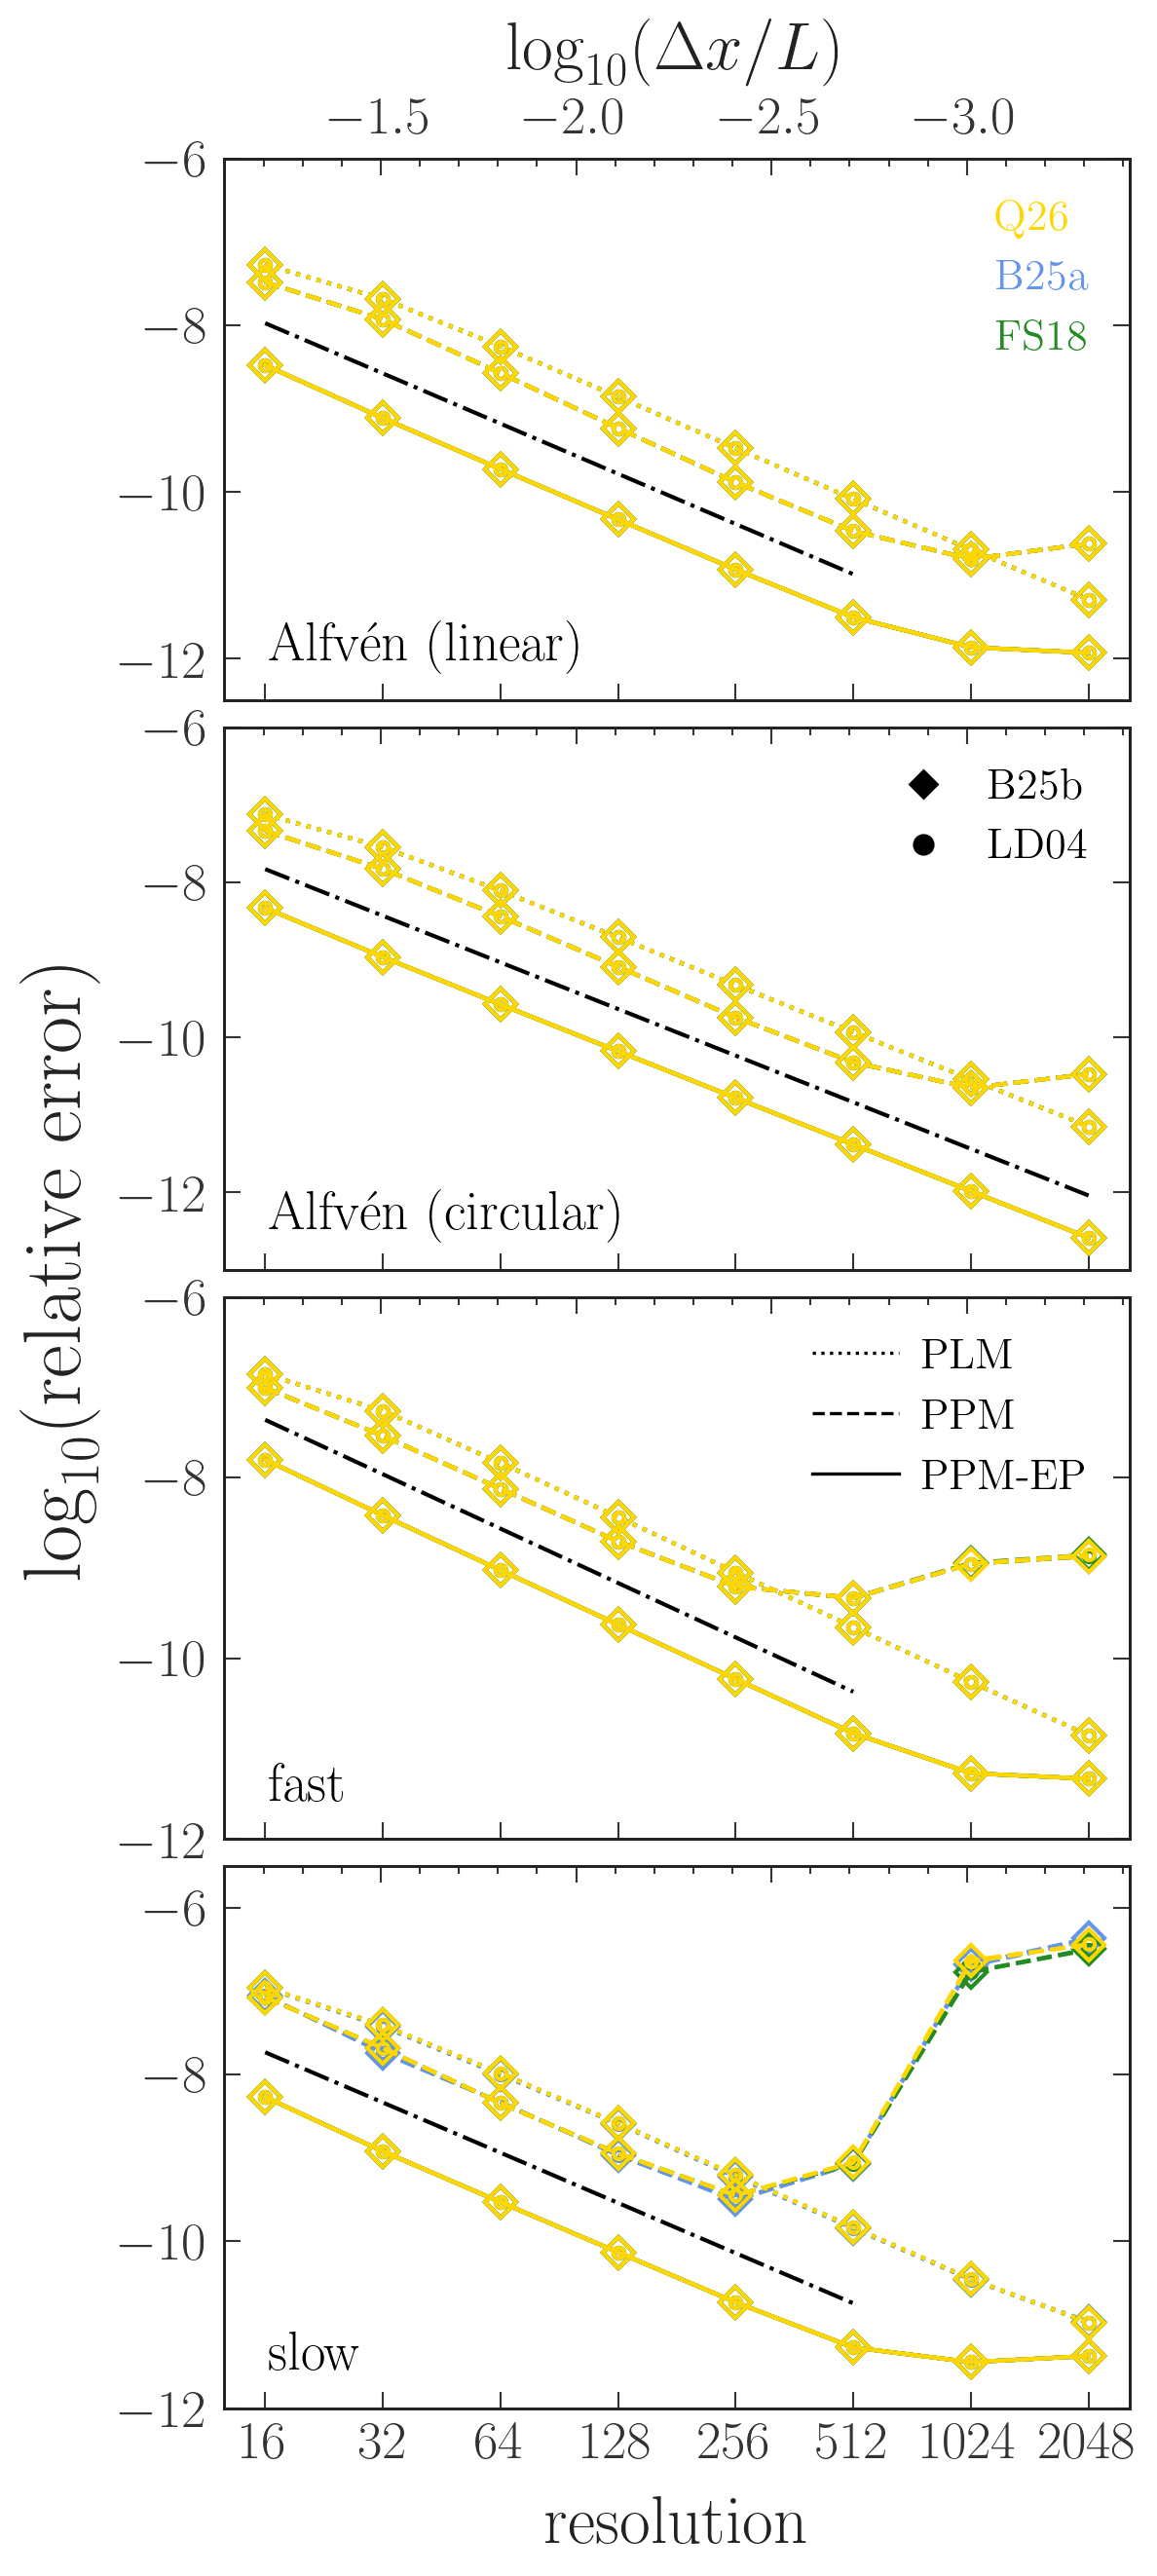
\includegraphics[width=0.55\linewidth]{figures/quokka-mhd/results/wave-convergence-grid-aligned.png}
    \caption{\DIFaddFL{Convergence of all 18 scheme combinations: EMF compute (indicated by colours; \sref{sec:methods:emf:compute}), EMF averaging (indicated by markers; \sref{sec:methods:emf:averaging}), and reconstruction (indicated by line style; \sref{sec:methods:flux}), against four wave-propagation scenarios: linearly-polarised Alfv\'en (first panel;
    \sref{sec:scheme-comparison:waves:alfven-linear}), circularly-polarised Alfv\'en (second panel; \sref{sec:scheme-comparison:waves:alfven-circular}), fast (third panel; \sref{sec:scheme-comparison:waves:fast}), and slow (last panel; \sref{sec:scheme-comparison:waves:slow}) waves. The relative error (\mbox{%DIFAUXCMD
\cref{eqn:error:relative}}\hskip0pt%DIFAUXCMD
) for each scheme combination is plotted against resolution (bottom axis), with the corresponding cell width shown on the top axis. A black dash-dotted line marks second-order convergence.}}
    \label{fig:waves:convergence}
\end{figure}

\DIFaddend For each simulation we measure the relative \DIFdelbegin \DIFdel{$L_1$ error . We define this by first defining the absolute $L_1$ error for each quantity $q$ in }\DIFdelend \DIFaddbegin \DIFadd{mean absolute error between the evolved and initial wave profiles, which we compute as follows: first we compute the mean absolute difference for each element $s$ of }\DIFaddend the state vector $\mVector{S}_\mathrm{c}$ as
\DIFdelbegin %DIFDELCMD < \begin{align}
%DIFDELCMD <     \mbox{error}_q
%DIFDELCMD <         = \frac{1}{N_q} \sum_{\forall i, j, k} \bigg|
%DIFDELCMD <             q_\mathrm{exact}\EvalAtH{i}{j}{k}
%DIFDELCMD <             - q_\mathrm{sim}\EvalAtH{i}{j}{k}
%DIFDELCMD <         \bigg|
%DIFDELCMD <     ,
%DIFDELCMD < \end{align}%%%
\DIFdelend \DIFaddbegin \begin{align}
    \mbox{error}_s
        = \frac{1}{N_s} \sum_{\forall i, j, k} \big|
            s_\mathrm{exact}\EvalAtH{i}{j}{k}
            - s_\mathrm{sim}\EvalAtH{i}{j}{k}
        \big|
    , \label{eqn:error:absolute}
\end{align}\DIFaddend
where \DIFdelbegin \DIFdel{$q_\mathrm{sim}\EvalAtH{i}{j}{k}$ and $q_\mathrm{exact}\EvalAtH{i}{j}{k}$ are the simulation-predicted and exact values at }\DIFdelend \DIFaddbegin \DIFadd{$s_\mathrm{sim}\EvalAtH{i}{j}{k}$ and $s_\mathrm{exact}\EvalAtH{i}{j}{k}$ are the simulated and analytically-exact values at the }\DIFaddend coordinate \DIFdelbegin \DIFdel{$(i, j, k)$ (the indexing is determined by whether $q$ is stored at cell-centres or face-centres), $N_q$ }\DIFdelend \DIFaddbegin \DIFadd{$\EvalAtH{i}{j}{k}$ where $s$ is stored (cell centre or face centre), respectively, $N_s$ }\DIFaddend is the number of cell centres or faces for that \DIFdelbegin \DIFdel{quantity}\DIFdelend \DIFaddbegin \DIFadd{element}\DIFaddend , and the sums run over all centres or faces. We \DIFdelbegin \DIFdel{similarly define }\DIFdelend \DIFaddbegin \DIFadd{then similarly compute }\DIFaddend the normalisation for that \DIFdelbegin \DIFdel{quantity as
}%DIFDELCMD < \begin{align}
%DIFDELCMD <     \mbox{norm}_q
%DIFDELCMD <         = \frac{1}{N_q} \sum_{\forall i, j, k} \bigg|
%DIFDELCMD <             q_\mathrm{exact}\EvalAtH{i}{j}{k}
%DIFDELCMD <         \bigg|
%DIFDELCMD <     ,
%DIFDELCMD < \end{align}%%%
\DIFdelend \DIFaddbegin \DIFadd{element as
}\begin{align}
    \mbox{norm}_s
        = \frac{1}{N_s} \sum_{\forall i, j, k} \big|
            s_\mathrm{exact}\EvalAtH{i}{j}{k}
        \big|
    , \label{eqn:error:normalisation}
\end{align}\DIFaddend
and \DIFdelbegin \DIFdel{then define the relative $L_1$ error as
}%DIFDELCMD < \begin{align}
%DIFDELCMD <     \epsilon
%DIFDELCMD <         = \rbrac{\frac{
%DIFDELCMD <                     \sum_{\forall q} \mbox{error}_q^2 N_q^2
%DIFDELCMD <                 }{
%DIFDELCMD <                     \sum_{\forall q} \mbox{norm}_q^2 N_q^2
%DIFDELCMD <             }}^{1/2}
%DIFDELCMD <     . \label{defn:error}
%DIFDELCMD < \end{align}%%%
\DIFdelend \DIFaddbegin \DIFadd{combine \mbox{%DIFAUXCMD
\cref{eqn:error:absolute} }\hskip0pt%DIFAUXCMD
and \mbox{%DIFAUXCMD
\cref{eqn:error:normalisation} }\hskip0pt%DIFAUXCMD
to compute the relative error across all elements of $\mVector{S}_\mathrm{c}$ as
}\begin{align}
    \mbox{relative error}
        = \rbrac{\frac{
                    \sum_{\forall s} \mbox{error}_s^2 N_s^2
                }{
                    \sum_{\forall s} \mbox{norm}_s^2 N_s^2
            }}^{1/2}
    . \label{eqn:error:relative}
\end{align}\DIFaddend
\DIFdelbegin \DIFdel{We plot this error }\DIFdelend \DIFaddbegin \DIFadd{This relative error is plotted in \mbox{%DIFAUXCMD
\cref{fig:waves:convergence} }\hskip0pt%DIFAUXCMD
for all 18 scheme combinations, }\DIFaddend as a function of resolution \DIFdelbegin \DIFdel{for all schemes in }%DIFDELCMD < \autoref{fig:linear_wave_convergence}%%%
\DIFdel{.
}%DIFDELCMD <

%DIFDELCMD < \begin{figure}
%DIFDELCMD <     \centering
%DIFDELCMD <     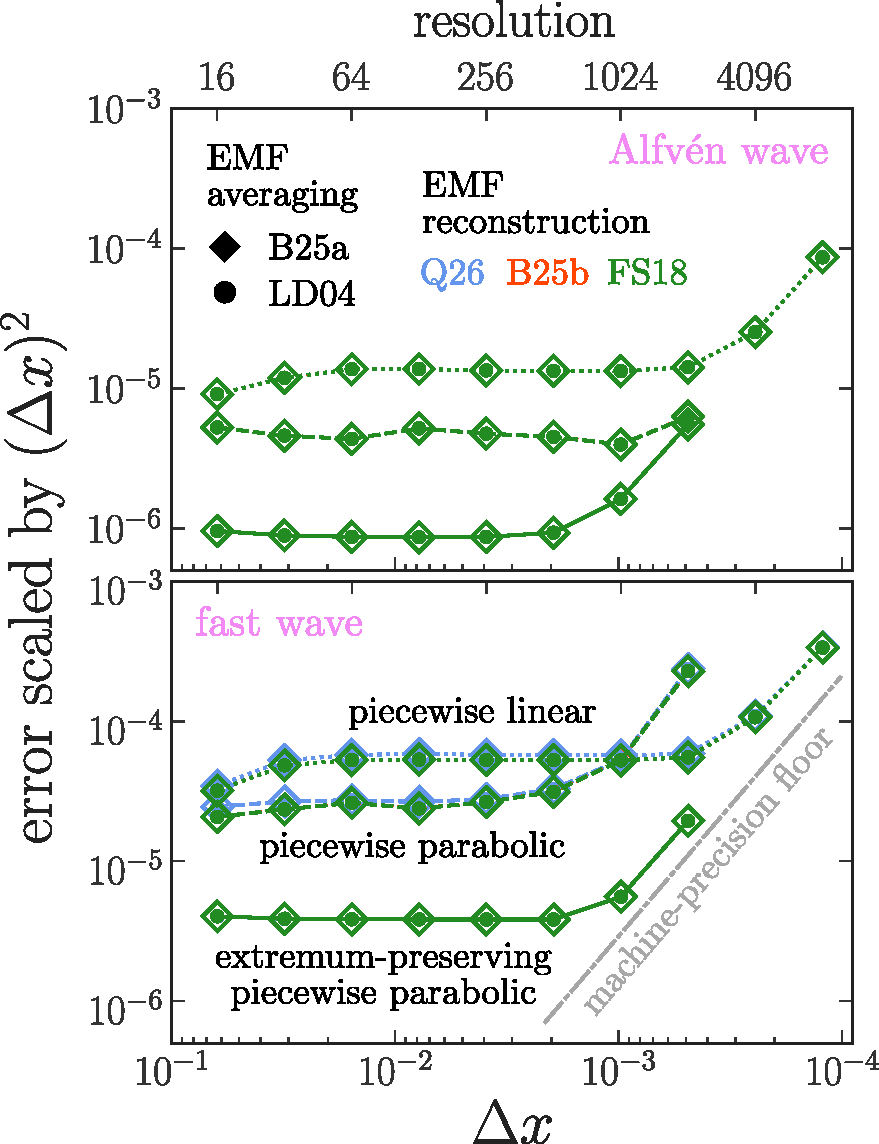
\includegraphics[width=0.65\linewidth]{figures/quokka-mhd/results/wave_convergence.pdf}
%DIFDELCMD <     %%%
%DIFDELCMD < \caption{%
{%DIFAUXCMD
\DIFdelFL{Convergence tests for Alfv\'en waves (top) and fast waves (bottom). In both panels, lines show the $L^1$ error (}%DIFDELCMD < \autoref{defn:error}%%%
\DIFdelFL{) compensated by grid spacing $(\Delta x)^2$, as a function of grid spacing; thus second-order convergence corresponds to a flat line in these plots. Blue, red, and green colours show the Q26, \mbox{%DIFAUXCMD
\citetalias{Balsara25a}}\hskip0pt%DIFAUXCMD
, and \mbox{%DIFAUXCMD
\citetalias{Felker18a} }\hskip0pt%DIFAUXCMD
EMF reconstruction schemes, respectively; diamond and circle markers indicate \mbox{%DIFAUXCMD
\citetalias{Londrillo04a} }\hskip0pt%DIFAUXCMD
and \mbox{%DIFAUXCMD
\citetalias{Balsara25b} }\hskip0pt%DIFAUXCMD
EMF averaging, respectively; dotted, dashed, and solid lines show PLM, PPM, and PPM-EP reconstruction, respectively. Because the results are nearly the same for all EMF averaging and reconstruction schemes, in many cases points are not visible because they are directly under other points. The dashed grey line labelled ``machine precision floor'' indicates where the error deviates from $\mathcal{O}((\Delta x)^{-2})$ scaling because the difference between the numerical and analytic solution is comparable to the numerical precision imposed by machine arithmetic.}}
    %DIFAUXCMD
%DIFDELCMD < \label{fig:linear_wave_convergence}
%DIFDELCMD < \end{figure}
%DIFDELCMD <

%DIFDELCMD < \begin{table}
%DIFDELCMD < \centering
%DIFDELCMD < %%%
%DIFDELCMD < \caption{%
{%DIFAUXCMD
\DIFdelFL{Best-fit parameters for error versus resolution (}%DIFDELCMD < \autoref{eq:err_vs_resolution}%%%
\DIFdelFL{) for different combinations of EMF reconstruction scheme, EMF averaging scheme, interpolation type, and wave type.
}%DIFDELCMD < \label{tab:linear_convergence}%%%
}
%DIFAUXCMD
%DIFDELCMD < \begin{tabular}{llrrr}
%DIFDELCMD < \hline\hline
%DIFDELCMD < %%%
\DIFdelFL{Reconstruction }%DIFDELCMD < & %%%
\DIFdelFL{Averaging }%DIFDELCMD < & %%%
\DIFdelFL{$\log \alpha_0$ }%DIFDELCMD < & %%%
\DIFdelFL{$\alpha_1$ }%DIFDELCMD < & %%%
\DIFdelFL{$\log \alpha_2$ }%DIFDELCMD < \\
%DIFDELCMD < \hline
%DIFDELCMD < %%%
%DIFDELCMD < \multicolumn{5}{c}{%
{%DIFAUXCMD
\DIFdelFL{Alfv\'en waves, PLM interpolation}} %DIFAUXCMD
%DIFDELCMD < \\
%DIFDELCMD < \hline
%DIFDELCMD < %%%
\DIFdelFL{B25 }%DIFDELCMD < & %%%
\DIFdelFL{B25 }%DIFDELCMD < & %%%
\DIFdelFL{$-5.231$ }%DIFDELCMD < & %%%
\DIFdelFL{1.840 }%DIFDELCMD < & %%%
\DIFdelFL{$-11.984$ }%DIFDELCMD < \\
%DIFDELCMD < %%%
\DIFdelFL{B25 }%DIFDELCMD < & %%%
\DIFdelFL{LD04 }%DIFDELCMD < & %%%
\DIFdelFL{$-5.231$ }%DIFDELCMD < & %%%
\DIFdelFL{1.840 }%DIFDELCMD < & %%%
\DIFdelFL{$-11.983$ }%DIFDELCMD < \\
%DIFDELCMD < %%%
\DIFdelFL{FS17 }%DIFDELCMD < & %%%
\DIFdelFL{B25 }%DIFDELCMD < & %%%
\DIFdelFL{$-5.231$ }%DIFDELCMD < & %%%
\DIFdelFL{1.840 }%DIFDELCMD < & %%%
\DIFdelFL{$-11.983$ }%DIFDELCMD < \\
%DIFDELCMD < %%%
\DIFdelFL{FS17 }%DIFDELCMD < & %%%
\DIFdelFL{LD04 }%DIFDELCMD < & %%%
\DIFdelFL{$-5.231$ }%DIFDELCMD < & %%%
\DIFdelFL{1.840 }%DIFDELCMD < & %%%
\DIFdelFL{$-11.983$ }%DIFDELCMD < \\
%DIFDELCMD < %%%
\DIFdelFL{Q26 }%DIFDELCMD < & %%%
\DIFdelFL{B25 }%DIFDELCMD < & %%%
\DIFdelFL{$-5.231$ }%DIFDELCMD < & %%%
\DIFdelFL{1.840 }%DIFDELCMD < & %%%
\DIFdelFL{$-11.983$ }%DIFDELCMD < \\
%DIFDELCMD < %%%
\DIFdelFL{Q26 }%DIFDELCMD < & %%%
\DIFdelFL{LD04 }%DIFDELCMD < & %%%
\DIFdelFL{$-5.231$ }%DIFDELCMD < & %%%
\DIFdelFL{1.840 }%DIFDELCMD < & %%%
\DIFdelFL{$-11.983$ }%DIFDELCMD < \\
%DIFDELCMD < \hline
%DIFDELCMD < %%%
%DIFDELCMD < \multicolumn{5}{c}{%
{%DIFAUXCMD
\DIFdelFL{Fast waves, PLM interpolation}} %DIFAUXCMD
%DIFDELCMD < \\
%DIFDELCMD < \hline
%DIFDELCMD < %%%
\DIFdelFL{B25b }%DIFDELCMD < & %%%
\DIFdelFL{B25a }%DIFDELCMD < & %%%
\DIFdelFL{$-4.742$ }%DIFDELCMD < & %%%
\DIFdelFL{1.791 }%DIFDELCMD < & %%%
\DIFdelFL{$-11.528$ }%DIFDELCMD < \\
%DIFDELCMD < %%%
\DIFdelFL{B25b }%DIFDELCMD < & %%%
\DIFdelFL{LD04 }%DIFDELCMD < & %%%
\DIFdelFL{$-4.742$ }%DIFDELCMD < & %%%
\DIFdelFL{1.791 }%DIFDELCMD < & %%%
\DIFdelFL{$-11.528$ }%DIFDELCMD < \\
%DIFDELCMD < %%%
\DIFdelFL{FS17 }%DIFDELCMD < & %%%
\DIFdelFL{B25a }%DIFDELCMD < & %%%
\DIFdelFL{$-4.742$ }%DIFDELCMD < & %%%
\DIFdelFL{1.791 }%DIFDELCMD < & %%%
\DIFdelFL{$-11.528$ }%DIFDELCMD < \\
%DIFDELCMD < %%%
\DIFdelFL{FS17 }%DIFDELCMD < & %%%
\DIFdelFL{LD04 }%DIFDELCMD < & %%%
\DIFdelFL{$-4.742$ }%DIFDELCMD < & %%%
\DIFdelFL{1.791 }%DIFDELCMD < & %%%
\DIFdelFL{$-11.528$ }%DIFDELCMD < \\
%DIFDELCMD < %%%
\DIFdelFL{Q26 }%DIFDELCMD < & %%%
\DIFdelFL{B25a }%DIFDELCMD < & %%%
\DIFdelFL{$-4.707$ }%DIFDELCMD < & %%%
\DIFdelFL{1.790 }%DIFDELCMD < & %%%
\DIFdelFL{$-11.640$ }%DIFDELCMD < \\
%DIFDELCMD < %%%
\DIFdelFL{Q26 }%DIFDELCMD < & %%%
\DIFdelFL{LD04 }%DIFDELCMD < & %%%
\DIFdelFL{$-4.707$ }%DIFDELCMD < & %%%
\DIFdelFL{1.790 }%DIFDELCMD < & %%%
\DIFdelFL{$-11.640$ }%DIFDELCMD < \\
%DIFDELCMD < \hline
%DIFDELCMD < %%%
%DIFDELCMD < \multicolumn{5}{c}{%
{%DIFAUXCMD
\DIFdelFL{Alfv\'en waves, PPM interpolation}} %DIFAUXCMD
%DIFDELCMD < \\
%DIFDELCMD < \hline
%DIFDELCMD < %%%
\DIFdelFL{B25b }%DIFDELCMD < & %%%
\DIFdelFL{B25a }%DIFDELCMD < & %%%
\DIFdelFL{$-5.197$ }%DIFDELCMD < & %%%
\DIFdelFL{2.070 }%DIFDELCMD < & %%%
\DIFdelFL{$-11.903$ }%DIFDELCMD < \\
%DIFDELCMD < %%%
\DIFdelFL{B25b }%DIFDELCMD < & %%%
\DIFdelFL{LD04 }%DIFDELCMD < & %%%
\DIFdelFL{$-5.197$ }%DIFDELCMD < & %%%
\DIFdelFL{2.070 }%DIFDELCMD < & %%%
\DIFdelFL{$-11.903$ }%DIFDELCMD < \\
%DIFDELCMD < %%%
\DIFdelFL{FS18 }%DIFDELCMD < & %%%
\DIFdelFL{B25a }%DIFDELCMD < & %%%
\DIFdelFL{$-5.197$ }%DIFDELCMD < & %%%
\DIFdelFL{2.070 }%DIFDELCMD < & %%%
\DIFdelFL{$-11.903$ }%DIFDELCMD < \\
%DIFDELCMD < %%%
\DIFdelFL{FS18 }%DIFDELCMD < & %%%
\DIFdelFL{LD04 }%DIFDELCMD < & %%%
\DIFdelFL{$-5.197$ }%DIFDELCMD < & %%%
\DIFdelFL{2.070 }%DIFDELCMD < & %%%
\DIFdelFL{$-11.903$ }%DIFDELCMD < \\
%DIFDELCMD < %%%
\DIFdelFL{Q26 }%DIFDELCMD < & %%%
\DIFdelFL{B25a }%DIFDELCMD < & %%%
\DIFdelFL{$-5.197$ }%DIFDELCMD < & %%%
\DIFdelFL{2.070 }%DIFDELCMD < & %%%
\DIFdelFL{$-11.903$ }%DIFDELCMD < \\
%DIFDELCMD < %%%
\DIFdelFL{Q26 }%DIFDELCMD < & %%%
\DIFdelFL{LD04 }%DIFDELCMD < & %%%
\DIFdelFL{$-5.197$ }%DIFDELCMD < & %%%
\DIFdelFL{2.070 }%DIFDELCMD < & %%%
\DIFdelFL{$-11.903$ }%DIFDELCMD < \\
%DIFDELCMD < \hline
%DIFDELCMD < %%%
%DIFDELCMD < \multicolumn{5}{c}{%
{%DIFAUXCMD
\DIFdelFL{Fast waves, PPM interpolation}} %DIFAUXCMD
%DIFDELCMD < \\
%DIFDELCMD < \hline
%DIFDELCMD < %%%
\DIFdelFL{B25b }%DIFDELCMD < & %%%
\DIFdelFL{B25a }%DIFDELCMD < & %%%
\DIFdelFL{$-4.759$ }%DIFDELCMD < & %%%
\DIFdelFL{1.936 }%DIFDELCMD < & %%%
\DIFdelFL{$-10.303$ }%DIFDELCMD < \\
%DIFDELCMD < %%%
\DIFdelFL{B25b }%DIFDELCMD < & %%%
\DIFdelFL{LD04 }%DIFDELCMD < & %%%
\DIFdelFL{$-4.758$ }%DIFDELCMD < & %%%
\DIFdelFL{1.937 }%DIFDELCMD < & %%%
\DIFdelFL{$-10.303$ }%DIFDELCMD < \\
%DIFDELCMD < %%%
\DIFdelFL{FS18 }%DIFDELCMD < & %%%
\DIFdelFL{B25a }%DIFDELCMD < & %%%
\DIFdelFL{$-4.760$ }%DIFDELCMD < & %%%
\DIFdelFL{1.936 }%DIFDELCMD < & %%%
\DIFdelFL{$-10.303$ }%DIFDELCMD < \\
%DIFDELCMD < %%%
\DIFdelFL{FS18 }%DIFDELCMD < & %%%
\DIFdelFL{LD04 }%DIFDELCMD < & %%%
\DIFdelFL{$-4.760$ }%DIFDELCMD < & %%%
\DIFdelFL{1.936 }%DIFDELCMD < & %%%
\DIFdelFL{$-10.303$ }%DIFDELCMD < \\
%DIFDELCMD < %%%
\DIFdelFL{Q26 }%DIFDELCMD < & %%%
\DIFdelFL{B25a }%DIFDELCMD < & %%%
\DIFdelFL{$-4.614$ }%DIFDELCMD < & %%%
\DIFdelFL{1.997 }%DIFDELCMD < & %%%
\DIFdelFL{$-10.298$ }%DIFDELCMD < \\
%DIFDELCMD < %%%
\DIFdelFL{Q26 }%DIFDELCMD < & %%%
\DIFdelFL{LD04 }%DIFDELCMD < & %%%
\DIFdelFL{$-4.613$ }%DIFDELCMD < & %%%
\DIFdelFL{1.998 }%DIFDELCMD < & %%%
\DIFdelFL{$-10.298$ }%DIFDELCMD < \\
%DIFDELCMD < \hline
%DIFDELCMD < %%%
%DIFDELCMD < \multicolumn{5}{c}{%
{%DIFAUXCMD
\DIFdelFL{Alfv\'en waves, PPM-EP interpolation}} %DIFAUXCMD
%DIFDELCMD < \\
%DIFDELCMD < \hline
%DIFDELCMD < %%%
\DIFdelFL{B25b }%DIFDELCMD < & %%%
\DIFdelFL{B25a }%DIFDELCMD < & %%%
\DIFdelFL{$-5.962$ }%DIFDELCMD < & %%%
\DIFdelFL{2.049 }%DIFDELCMD < & %%%
\DIFdelFL{$-11.883$ }%DIFDELCMD < \\
%DIFDELCMD < %%%
\DIFdelFL{B25b }%DIFDELCMD < & %%%
\DIFdelFL{LD04 }%DIFDELCMD < & %%%
\DIFdelFL{$-5.962$ }%DIFDELCMD < & %%%
\DIFdelFL{2.049 }%DIFDELCMD < & %%%
\DIFdelFL{$-11.883$ }%DIFDELCMD < \\
%DIFDELCMD < %%%
\DIFdelFL{FS17 }%DIFDELCMD < & %%%
\DIFdelFL{B25a }%DIFDELCMD < & %%%
\DIFdelFL{$-5.962$ }%DIFDELCMD < & %%%
\DIFdelFL{2.049 }%DIFDELCMD < & %%%
\DIFdelFL{$-11.883$ }%DIFDELCMD < \\
%DIFDELCMD < %%%
\DIFdelFL{FS17 }%DIFDELCMD < & %%%
\DIFdelFL{LD04 }%DIFDELCMD < & %%%
\DIFdelFL{$-5.962$ }%DIFDELCMD < & %%%
\DIFdelFL{2.049 }%DIFDELCMD < & %%%
\DIFdelFL{$-11.883$ }%DIFDELCMD < \\
%DIFDELCMD < %%%
\DIFdelFL{Q26 }%DIFDELCMD < & %%%
\DIFdelFL{B25a }%DIFDELCMD < & %%%
\DIFdelFL{$-5.962$ }%DIFDELCMD < & %%%
\DIFdelFL{2.049 }%DIFDELCMD < & %%%
\DIFdelFL{$-11.883$ }%DIFDELCMD < \\
%DIFDELCMD < %%%
\DIFdelFL{Q26 }%DIFDELCMD < & %%%
\DIFdelFL{LD04 }%DIFDELCMD < & %%%
\DIFdelFL{$-5.962$ }%DIFDELCMD < & %%%
\DIFdelFL{2.049 }%DIFDELCMD < & %%%
\DIFdelFL{$-11.883$ }%DIFDELCMD < \\
%DIFDELCMD < \hline
%DIFDELCMD < %%%
%DIFDELCMD < \multicolumn{5}{c}{%
{%DIFAUXCMD
\DIFdelFL{Fast waves, PPM-EP interpolation}} %DIFAUXCMD
%DIFDELCMD < \\
%DIFDELCMD < \hline
%DIFDELCMD < %%%
\DIFdelFL{B25b }%DIFDELCMD < & %%%
\DIFdelFL{B25a }%DIFDELCMD < & %%%
\DIFdelFL{$-5.351$ }%DIFDELCMD < & %%%
\DIFdelFL{2.035 }%DIFDELCMD < & %%%
\DIFdelFL{$-11.343$ }%DIFDELCMD < \\
%DIFDELCMD < %%%
\DIFdelFL{B25b }%DIFDELCMD < & %%%
\DIFdelFL{LD04 }%DIFDELCMD < & %%%
\DIFdelFL{$-5.351$ }%DIFDELCMD < & %%%
\DIFdelFL{2.035 }%DIFDELCMD < & %%%
\DIFdelFL{$-11.343$ }%DIFDELCMD < \\
%DIFDELCMD < %%%
\DIFdelFL{FS17 }%DIFDELCMD < & %%%
\DIFdelFL{B25a }%DIFDELCMD < & %%%
\DIFdelFL{$-5.351$ }%DIFDELCMD < & %%%
\DIFdelFL{2.035 }%DIFDELCMD < & %%%
\DIFdelFL{$-11.343$ }%DIFDELCMD < \\
%DIFDELCMD < %%%
\DIFdelFL{FS17 }%DIFDELCMD < & %%%
\DIFdelFL{LD04 }%DIFDELCMD < & %%%
\DIFdelFL{$-5.351$ }%DIFDELCMD < & %%%
\DIFdelFL{2.035 }%DIFDELCMD < & %%%
\DIFdelFL{$-11.343$ }%DIFDELCMD < \\
%DIFDELCMD < %%%
\DIFdelFL{Q26 }%DIFDELCMD < & %%%
\DIFdelFL{B25a }%DIFDELCMD < & %%%
\DIFdelFL{$-5.352$ }%DIFDELCMD < & %%%
\DIFdelFL{2.035 }%DIFDELCMD < & %%%
\DIFdelFL{$-11.343$ }%DIFDELCMD < \\
%DIFDELCMD < %%%
\DIFdelFL{Q26 }%DIFDELCMD < & %%%
\DIFdelFL{LD04 }%DIFDELCMD < & %%%
\DIFdelFL{$-5.352$ }%DIFDELCMD < & %%%
\DIFdelFL{2.035 }%DIFDELCMD < & %%%
\DIFdelFL{$-11.343$ }%DIFDELCMD < \\
%DIFDELCMD < \hline\hline
%DIFDELCMD < \end{tabular}
%DIFDELCMD < \end{table}
%DIFDELCMD <

%DIFDELCMD < %%%
\DIFdel{As the plot shows}\DIFdelend \DIFaddbegin \DIFadd{(on the lower x-axis}\DIFaddend , and as \DIFdelbegin \DIFdel{expected, }\DIFdelend \DIFaddbegin \DIFadd{cell spacing on the upper x-axis). Broadly, for all schemes and waves, }\DIFaddend we find that the error decreases as \DIFdelbegin \DIFdel{a powerlaw in the $N$, for small $N$, before reaching a minimum error imposed by the finite precision of machine arithmetic and / or the fact that the analytic solution is only accurate to first order in the perturbation amplitude $\delta_{a}$. We therefore carry out a simple $\chi^2$ fit for the $L^1$ errors we measure at different resolutions of each scheme, using a functional form
}%DIFDELCMD < \begin{align}
%DIFDELCMD <     \epsilon(N)
%DIFDELCMD <         = \rbrac{\rbrac{\alpha_0 N^{-\alpha_1}}^2 + \alpha_2^2}^{1/2}
%DIFDELCMD <     , \label{eq:err_vs_resolution}
%DIFDELCMD < \end{align}
%DIFDELCMD < %%%
\DIFdel{where the error normalisation $\alpha_0$, floor value $\alpha_2$, and convergence rate $\alpha_1$ are parameter to be fit. We report the best-fit values for all combinations of scheme in }%DIFDELCMD < \autoref{tab:linear_convergence}%%%
\DIFdel{. }%DIFDELCMD <

%DIFDELCMD < %%%
\DIFdel{As the figure and tabulated data show, the error normalisations, floor values, and convergence rates are nearly identical for all combinations of EMF reconstruction and averaging scheme. These quantities depend only on the reconstruction type (PLM, PPM, or }\DIFdelend \DIFaddbegin \DIFadd{resolution increases, at a rate that is second-order. This is expected, since all three reconstruction schemes are second-order in space, or higher, and our time stepping strategy is second-order in time, which bottlenecks PPM and }\DIFaddend PPM-EP \DIFdelbegin \DIFdel{), and all schemes achieving roughly }\DIFdelend \DIFaddbegin \DIFadd{to }\DIFaddend second-order \DIFdelbegin \DIFdel{convergence, $\alpha_1 \approx 2$ -- which is expected behaviour given that we have not implemented the extra interpolation steps that would be required to reach higher-order \mbox{%DIFAUXCMD
\citep[e.g.,][]{Felker18a, Balsara25a}}\hskip0pt%DIFAUXCMD
. The order of interpolation mostly appear to affect the normalisation of the error scaling.
We therefore conclude that all of }\DIFdelend \DIFaddbegin \DIFadd{overall. PPM-EP converges cleanly to the numerical-precision floor, reaching a similar relative error to }\DIFaddend the \DIFdelbegin \DIFdel{reconstruction and averaging schemes perform nearly-identically for linear waves, and that the differences in interpolation scheme behave as expected for each of them}\DIFdelend \DIFaddbegin \DIFadd{more diffusive PLM scheme at roughly $4\times$ lower resolution. Plain PPM sits between these two reconstruction schemes through to moderate resolution, but at higher resolution its relative error departs from smooth convergence.
}

\DIFadd{Rather than converging to the numerical-precision floor, plain PPM's relative error reaches a problem-dependent minimum between $10^{-11}$ and $10^{-9}$, and then grows monotonically with increasing resolution. This effect is mild for both linearly and circularly polarised Alfv\'en waves alike, slightly more apparent in the fast magnetosonic wave, and very pronounced in the slow magnetosonic wave. Despite the degradation, this is not a numerical instability but an accuracy defect of the reconstruction scheme: a genuine instability would show unbounded growth, whereas here the solution remains bounded and conserves energy throughout. This is a well-known result of the Colella-Woodward monotonicity limiter \mbox{%DIFAUXCMD
\citep{Colella84a}}\hskip0pt%DIFAUXCMD
, which cannot distinguish a smooth, well-resolved extremum from a genuine discontinuity, so it clips the wave crests, coherently damping the amplitude once the profile is adequately resolved; this is the same clipping-induced dissipation effect documented for smooth, periodic profiles by \mbox{%DIFAUXCMD
\citet{Felker18a}}\hskip0pt%DIFAUXCMD
. The extremum-preserving version of PPM \mbox{%DIFAUXCMD
\citep[PPM-EP;][]{Rider07a} }\hskip0pt%DIFAUXCMD
relaxes this limiter at smooth extrema and recovers clean convergence to the machine precision.
}

\DIFadd{This pathology is specific to smooth, linear, advection-dominated flows, where extrema of waves accumulate the limiter's clipping. Real problems are rarely as pristine as single-frequency waves: discontinuities and non-linear structures are exactly what the limiter exists to stabilise against. Indeed, of all the tests in this chapter, this convergence study is the only one where this artefact of PPM appears; see \sref{sec:scheme-comparison:shocks} and \sref{sec:scheme-comparison:orszag-tang} for more detailed analysis of plain PPM and PPM-EP}\DIFaddend .

\subsection{\DIFdelbegin \DIFdel{Magnetised }\DIFdelend \DIFaddbegin \DIFadd{Resolving magnetised }\DIFaddend shocks\DIFdelbegin \DIFdel{: the Brio-Wu shock tube}\DIFdelend }
\DIFdelbegin %DIFDELCMD < \label{sec:performance:brio-wu}
%DIFDELCMD < %%%
\DIFdelend \DIFaddbegin \label{sec:scheme-comparison:shocks}
\DIFaddend

\DIFdelbegin \DIFdel{Our second comparison between the schemes is the classic \mbox{%DIFAUXCMD
\citet{Brio88a} }\hskip0pt%DIFAUXCMD
shock tube test. In this test we start with a discontinuity at $x=0$, with the states at $x<0$ and $x>0$ defined by, respectively,
}%DIFDELCMD < \begin{align}
%DIFDELCMD <     \begin{Bmatrix}
%DIFDELCMD <         \rho \\
%DIFDELCMD <         u_1 \\
%DIFDELCMD <         u_2 \\
%DIFDELCMD <         u_3 \\
%DIFDELCMD <         e_\mathrm{tot} \\
%DIFDELCMD <         b_1 \\
%DIFDELCMD <         b_2 \\
%DIFDELCMD <         b_3
%DIFDELCMD <     \end{Bmatrix}_L
%DIFDELCMD <         = \begin{Bmatrix}
%DIFDELCMD <             1 \\
%DIFDELCMD <             0 \\
%DIFDELCMD <             0 \\
%DIFDELCMD <             0 \\
%DIFDELCMD <             1.78125\\
%DIFDELCMD <             0.75 \\
%DIFDELCMD <             1 \\
%DIFDELCMD <             0
%DIFDELCMD <         \end{Bmatrix}
%DIFDELCMD <     \, \, \mbox{and}\, \,
%DIFDELCMD <     \begin{Bmatrix}
%DIFDELCMD <         \rho \\
%DIFDELCMD <         u_1 \\
%DIFDELCMD <         u_2 \\
%DIFDELCMD <         u_3 \\
%DIFDELCMD <         e_\mathrm{tot} \\
%DIFDELCMD <         b_1 \\
%DIFDELCMD <         b_2 \\
%DIFDELCMD <         b_3
%DIFDELCMD <     \end{Bmatrix}_R
%DIFDELCMD <         = \begin{Bmatrix}
%DIFDELCMD <             0.125 \\
%DIFDELCMD <             0 \\
%DIFDELCMD <             0 \\
%DIFDELCMD <             0 \\
%DIFDELCMD <             0.88125\\
%DIFDELCMD <             0.75 \\
%DIFDELCMD <             -1\\
%DIFDELCMD <             0
%DIFDELCMD <         \end{Bmatrix}
%DIFDELCMD < \end{align}
%DIFDELCMD < %%%
\DIFdel{The gas is adiabatic with index $\gamma=2$. We run this problem at a resolution of $512 \times 8 \times 8$ to time $t = 0.1$ over a domain $x_1 \in [0, 1]$ using all six possible }\DIFdelend \DIFaddbegin \DIFadd{Next we compare our suite of schemes against two classical 1D MHD shock tube problems: first, the \mbox{%DIFAUXCMD
\citet{RyuJones95a} }\hskip0pt%DIFAUXCMD
test and then the \mbox{%DIFAUXCMD
\citet{Brio88a} }\hskip0pt%DIFAUXCMD
test. At moderate resolutions, these tests together provide complementary validation of the Riemann solver. The Ryu-Jones shock tube validates that all seven MHD wave families can be resolved, and the Brio-Wu shock tube validates that a compound wave, which is not present in the Ryu-Jones test, can also be resolved by the solver.
}

\DIFadd{In both tests we consider adiabatic flows in a domain spanning $x_0 \in [-0.5, 0.5]$, with an initial discontinuity at $x_\mathrm{shock} = 0$; since the resulting evolution is self-similar (the speed of every wave is constant in time), we are free to compare our schemes at any time, as long as it is before the fastest wave reaches the domain boundary. We therefore choose the final snapshot in our time series that meets this criterion.
}

\DIFadd{We test all six }\DIFaddend combinations of EMF \DIFdelbegin \DIFdel{reconstruction and }\DIFdelend \DIFaddbegin \DIFadd{compute scheme (\sref{sec:methods:emf:compute}) and EMF }\DIFaddend averaging scheme (\DIFdelbegin \DIFdel{\mbox{%DIFAUXCMD
\citetalias{Felker18a}}\hskip0pt%DIFAUXCMD
, \mbox{%DIFAUXCMD
\citetalias{Balsara25a}}\hskip0pt%DIFAUXCMD
, and }\DIFdelend \DIFaddbegin \DIFadd{\sref{sec:methods:emf:averaging}), coupled with PPM-EP reconstruction. We also validate our LLF Riemann solver (which is used in our FOFC strategy; see \sref{sec:methods:time-stepping}) by substituting it in place of HLLD, coupled with the }\DIFaddend Q26 \DIFdelbegin \DIFdel{, together with \mbox{%DIFAUXCMD
\citetalias{Londrillo04a} }\hskip0pt%DIFAUXCMD
and \mbox{%DIFAUXCMD
\citetalias{Balsara25b}}\hskip0pt%DIFAUXCMD
}\DIFdelend \DIFaddbegin \DIFadd{compute, \mbox{%DIFAUXCMD
\citetalias{Balsara25b} }\hskip0pt%DIFAUXCMD
averaging, and PPM-EP reconstruction schemes. Finally, following the findings in \sref{sec:scheme-comparison:waves} (concerning degraded solutions when using PPM reconstruction), we also consider a run with the same EMF scheme combination (Q26 with \mbox{%DIFAUXCMD
\citetalias{Balsara25b}}\hskip0pt%DIFAUXCMD
), this time coupled with PPM (and the default HLLD solver}\DIFaddend ). We \DIFdelbegin \DIFdel{use PPM-EP interpolation }\DIFdelend \DIFaddbegin \DIFadd{discuss the results of both tests, }\DIFaddend for all of these \DIFdelbegin \DIFdel{tests}\DIFdelend \DIFaddbegin \DIFadd{scheme combinations, together in \sref{sec:scheme-comparison:shocks:discussion}}\DIFaddend .

\DIFdelbegin \DIFdel{We show the results in }%DIFDELCMD < \autoref{fig:bw-profiles}%%%
\DIFdel{, comparing to a reference solution from \mbox{%DIFAUXCMD
\citetalias{Felker18a}}\hskip0pt%DIFAUXCMD
.
We find that all schemes reproduce the reference solution extremely well, properly capturing all of the }\DIFdelend \DIFaddbegin \subsubsection{\DIFadd{The Ryu \& Jones (1995) shock tube}}
\label{sec:scheme-comparison:shocks:ryu-jones}

\DIFadd{For this test we set $\gamma=5/3$ and initialise the left ($x_0 \leq x_\mathrm{shock}$) and right ($x_0 > x_\mathrm{shock}$) halves of the domain with the states
}\begin{align}
\scalebox{0.95}{%
\mbox{%DIFAUXCMD
$\displaystyle
    \mVector{S}_\mathrm{c}^{[L]}
        = \begin{Bmatrix}
                \rho \\
                u_0 \\
                u_1 \\
                u_2 \\
                p \\
                b_0 \\
                b_1 \\
                b_2
            \end{Bmatrix}
        = \begin{Bmatrix}
                1.08 \\
                1.2 \\
                0.01 \\
                0.5 \\
                0.95 \\
                2/\sqrt{4\pi} \\
                3.6/\sqrt{4\pi} \\
                2/\sqrt{4\pi}
            \end{Bmatrix}
    , \qquad
    \mVector{S}_\mathrm{c}^{[R]}
        = \begin{Bmatrix}
                \rho \\
                u_0 \\
                u_1 \\
                u_2 \\
                p \\
                b_0 \\
                b_1 \\
                b_2
            \end{Bmatrix}
        = \begin{Bmatrix}
                1 \\
                0 \\
                0 \\
                0 \\
                1 \\
                2/\sqrt{4\pi} \\
                4/\sqrt{4\pi} \\
                2/\sqrt{4\pi}
            \end{Bmatrix}
$
}%DIFAUXCMD
}
    .
\end{align}
\DIFadd{We run this problem at a resolution of $512$ until $t=0.2$; we use a higher resolution than for the Brio-Wu test below, since this test has far richer wave structures and requires high resolution for numerical differences between the schemes to be visually discernible. We then compare every scheme to the exact solution at each cell position, computed using an exact Riemann solver \mbox{%DIFAUXCMD
\citep{Kriel26a}}\hskip0pt%DIFAUXCMD
.
}

\subsubsection{\DIFadd{The Brio \& Wu (1988) shock tube}}
\label{sec:scheme-comparison:shocks:brio-wu}

\DIFadd{For this test we set $\gamma=2$ and initialise the left ($x_0 \leq x_\mathrm{shock}$) and right ($x_0 > x_\mathrm{shock}$) halves of the domain with the states
}\begin{align}
\scalebox{0.95}{%
\mbox{%DIFAUXCMD
$\displaystyle
    \mVector{S}_\mathrm{c}^{[L]}
        = \begin{Bmatrix}
                \rho \\
                u_0 \\
                u_1 \\
                u_2 \\
                p \\
                b_0 \\
                b_1 \\
                b_2
            \end{Bmatrix}
        = \begin{Bmatrix}
                1 \\
                0 \\
                0 \\
                0 \\
                1 \\
                0.75 \\
                1 \\
                0
            \end{Bmatrix}
    , \qquad
    \mVector{S}_\mathrm{c}^{[R]}
        = \begin{Bmatrix}
                \rho \\
                u_0 \\
                u_1 \\
                u_2 \\
                p \\
                b_0 \\
                b_1 \\
                b_2
            \end{Bmatrix}
        = \begin{Bmatrix}
                0.125 \\
                0 \\
                0 \\
                0 \\
                0.1 \\
                0.75 \\
                -1 \\
                0
            \end{Bmatrix}
$
}%DIFAUXCMD
}
    .
\end{align}
\DIFadd{We run this problem at a resolution of $256$ until $t = 0.1$. Unlike the Ryu-Jones test, the transverse magnetic field for this test is coplanar (}\ie \DIFadd{$b_2 = 0$ on both sides of the discontinuity), which means the rotational discontinuities of the exact 7-wave solution are degenerate. Since we do not have an exact solution available, we instead use, as our reference solution, a simulation using Q26 with \mbox{%DIFAUXCMD
\citetalias{Balsara25b} }\hskip0pt%DIFAUXCMD
and PPM-EP, run at a much higher resolution of $8192$.
}

\subsubsection{\DIFadd{Analysis of shock-tube results}}
\label{sec:scheme-comparison:shocks:discussion}

\begin{figure*}
    \centering
    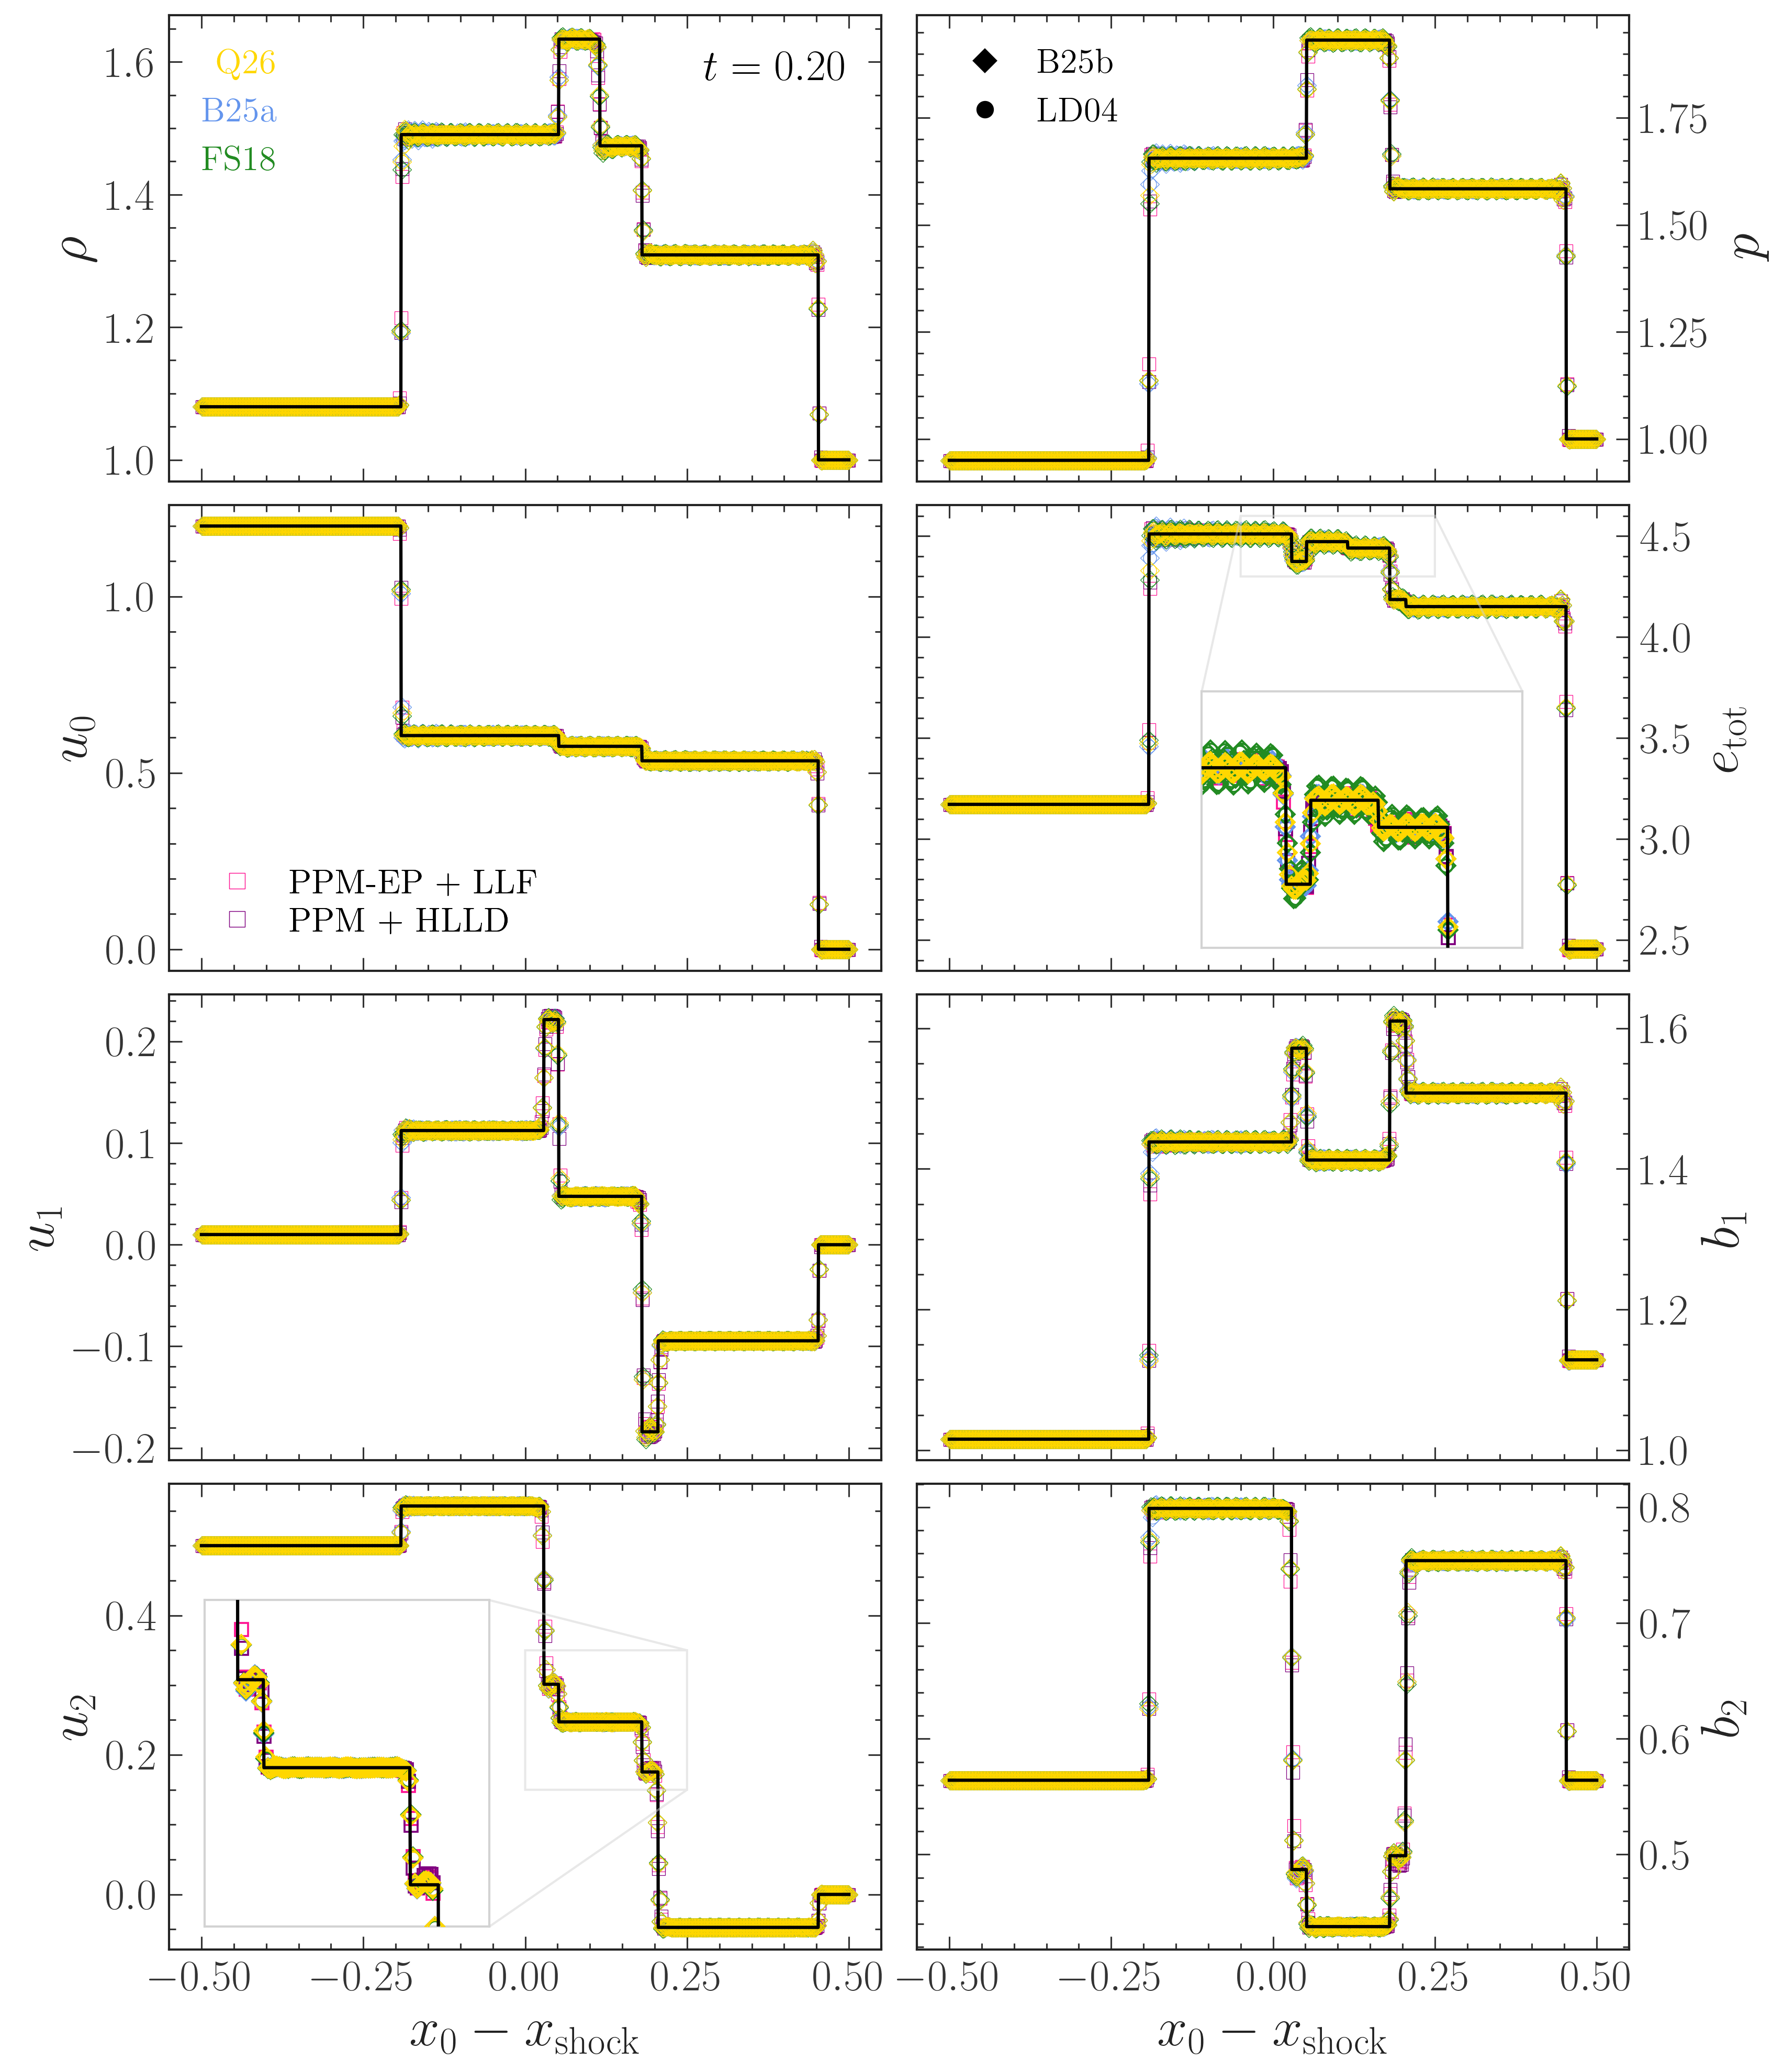
\includegraphics[width=\linewidth]{figures/quokka-mhd/results/ryu-jones-2a-shock-tube-scheme-comparison.png}
    \caption{\DIFaddFL{The \mbox{%DIFAUXCMD
\citet{RyuJones95a} }\hskip0pt%DIFAUXCMD
shock tube test (\sref{sec:scheme-comparison:shocks:ryu-jones}) compared across 6 EMF scheme combinations run at $N = 512$ with PPM-EP reconstruction and our HLLD Riemann solver: EMF compute (indicated by colour; \sref{sec:methods:emf:compute}) and EMF averaging (indicated by marker; \sref{sec:methods:emf:averaging}). We also consider two more scheme combinations, both paired with Q26 compute and \mbox{%DIFAUXCMD
\citetalias{Balsara25b} }\hskip0pt%DIFAUXCMD
averaging: our LLF Riemann solver with PPM-EP reconstruction (pink squares), and HLLD with plain PPM reconstruction (purple squares). Each panel shows the profile of key quantities at $t = 0.20$ along $x_0$, with the exact solution (black line) computed with the Riemann solver of \mbox{%DIFAUXCMD
\citet{Kriel26a}}\hskip0pt%DIFAUXCMD
.}}
    \label{fig:ryu-jones-profiles}
\end{figure*}

\begin{figure*}
    \centering
    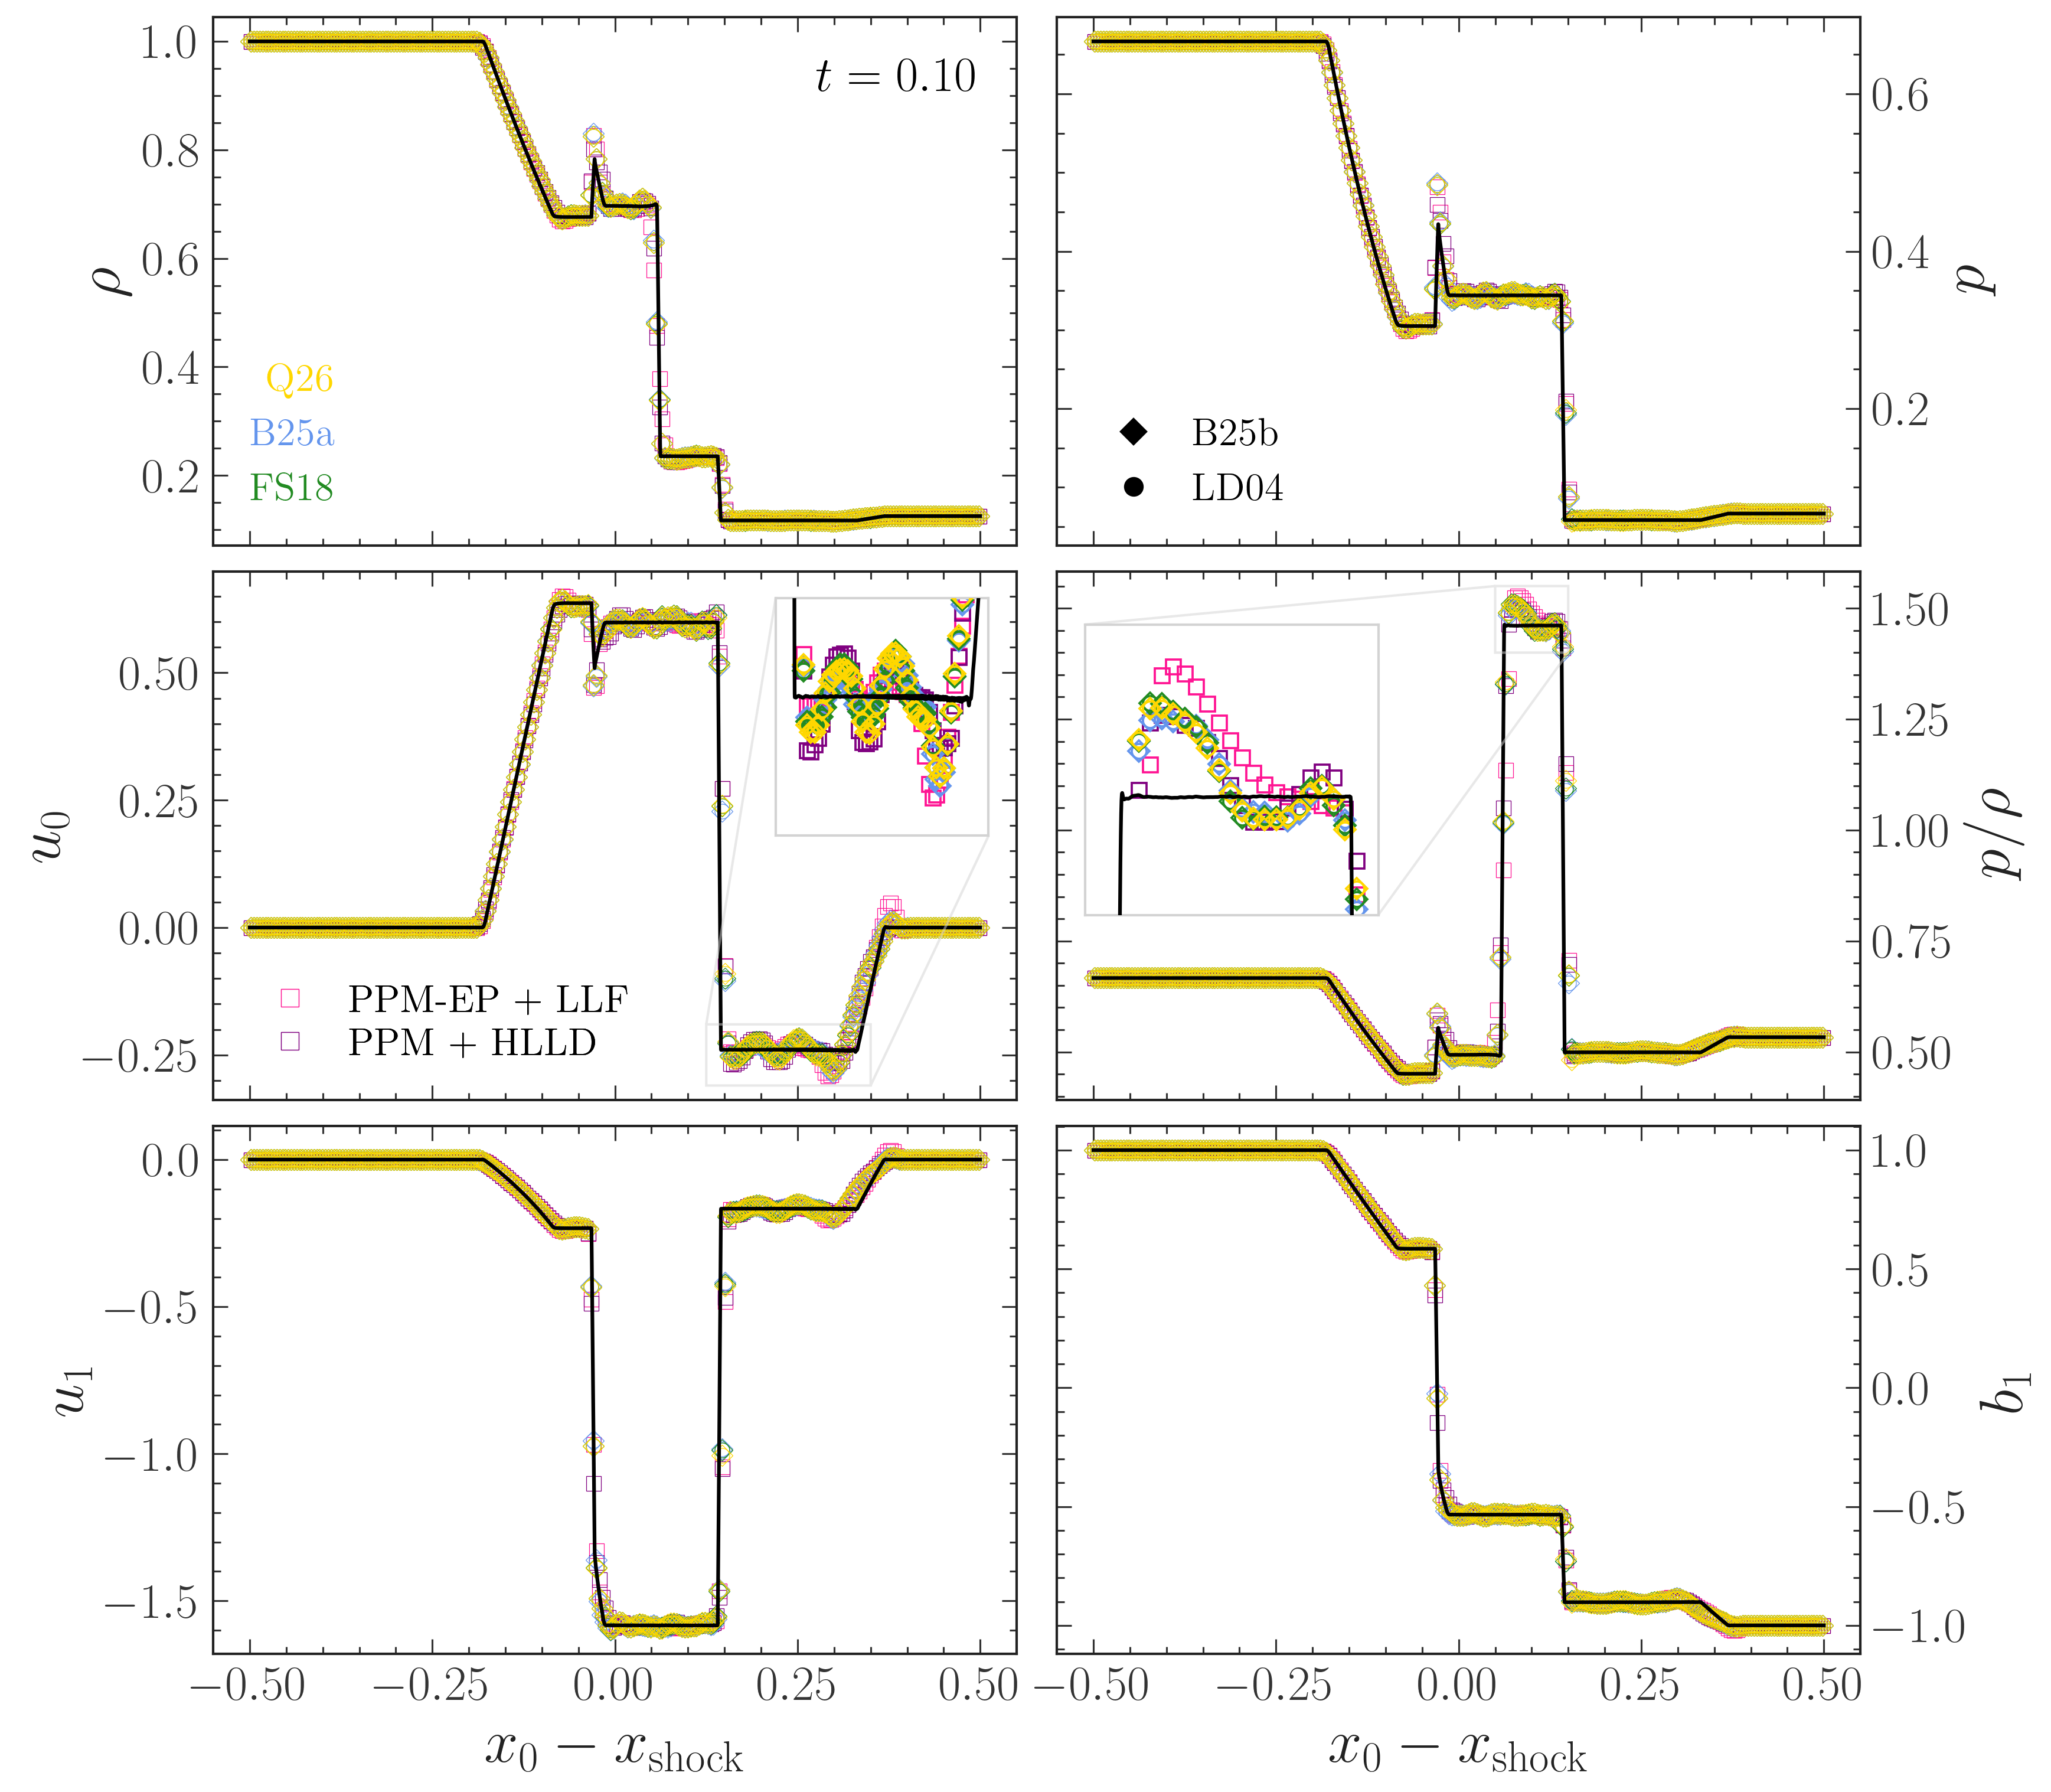
\includegraphics[width=\linewidth]{figures/quokka-mhd/results/brio-wu-shock-tube-scheme-comparison.png}
    \caption{\DIFaddFL{The \mbox{%DIFAUXCMD
\citet{Brio88a} }\hskip0pt%DIFAUXCMD
shock tube test (\sref{sec:scheme-comparison:shocks:brio-wu}) run at $N = 256$, across the same scheme combinations as \mbox{%DIFAUXCMD
\cref{fig:ryu-jones-profiles}}\hskip0pt%DIFAUXCMD
, showing profiles of key quantities at $t = 0.1$. A reference solution (black line) is found by running the problem with Q26 compute, \mbox{%DIFAUXCMD
\citetalias{Balsara25b} }\hskip0pt%DIFAUXCMD
averaging, and PPM-EP reconstruction at $N = 8192$.}}
    \label{fig:brio-wu-profiles}
\end{figure*}

\DIFadd{As in \mbox{%DIFAUXCMD
\cref{sec:scheme-comparison:waves}}\hskip0pt%DIFAUXCMD
, every scheme combination we test agrees closely overall, resolving the same wave structures in both shock tubes (\mbox{%DIFAUXCMD
\cref{fig:ryu-jones-profiles,fig:brio-wu-profiles}}\hskip0pt%DIFAUXCMD
) with no qualitative disagreement or missing wave }\DIFaddend features. The choice of \DIFdelbegin \DIFdel{EMF averaging scheme makes no noticeable difference. The EMF reconstruction scheme matters slightly more, with the Q26 scheme showing somewhat }\DIFdelend \DIFaddbegin \DIFadd{Riemann solver and EMF compute scheme each has only a modest effect on the outcome: LLF (pink squares) does not resolve the contact discontinuity as well as HLLD (all other points), and as a result shows }\DIFaddend more ringing in the \DIFdelbegin \DIFdel{region between the intermediate compound wave and the contact discontinuity (see inset in }%DIFDELCMD < \autoref{fig:bw-profiles}%%%
\DIFdel{). However, the differences are small }\DIFdelend \DIFaddbegin \DIFadd{Brio-Wu $p/\rho$ profile (which is proportional to plasma temperature). Among the EMF compute schemes, Q26 shows the least ringing, which is most visible in the $e_\mathrm{tot}$ profile of the Ryu-Jones test. Similarly, the choice of reconstruction order makes little difference: both PPM and PPM-EP agree closely across all quantities in both tests, with only small ringing-related differences visible in the $u_0$ profile of the Brio-Wu test}\DIFaddend .

\DIFdelbegin %DIFDELCMD < \begin{figure}
%DIFDELCMD <     \centering
%DIFDELCMD <     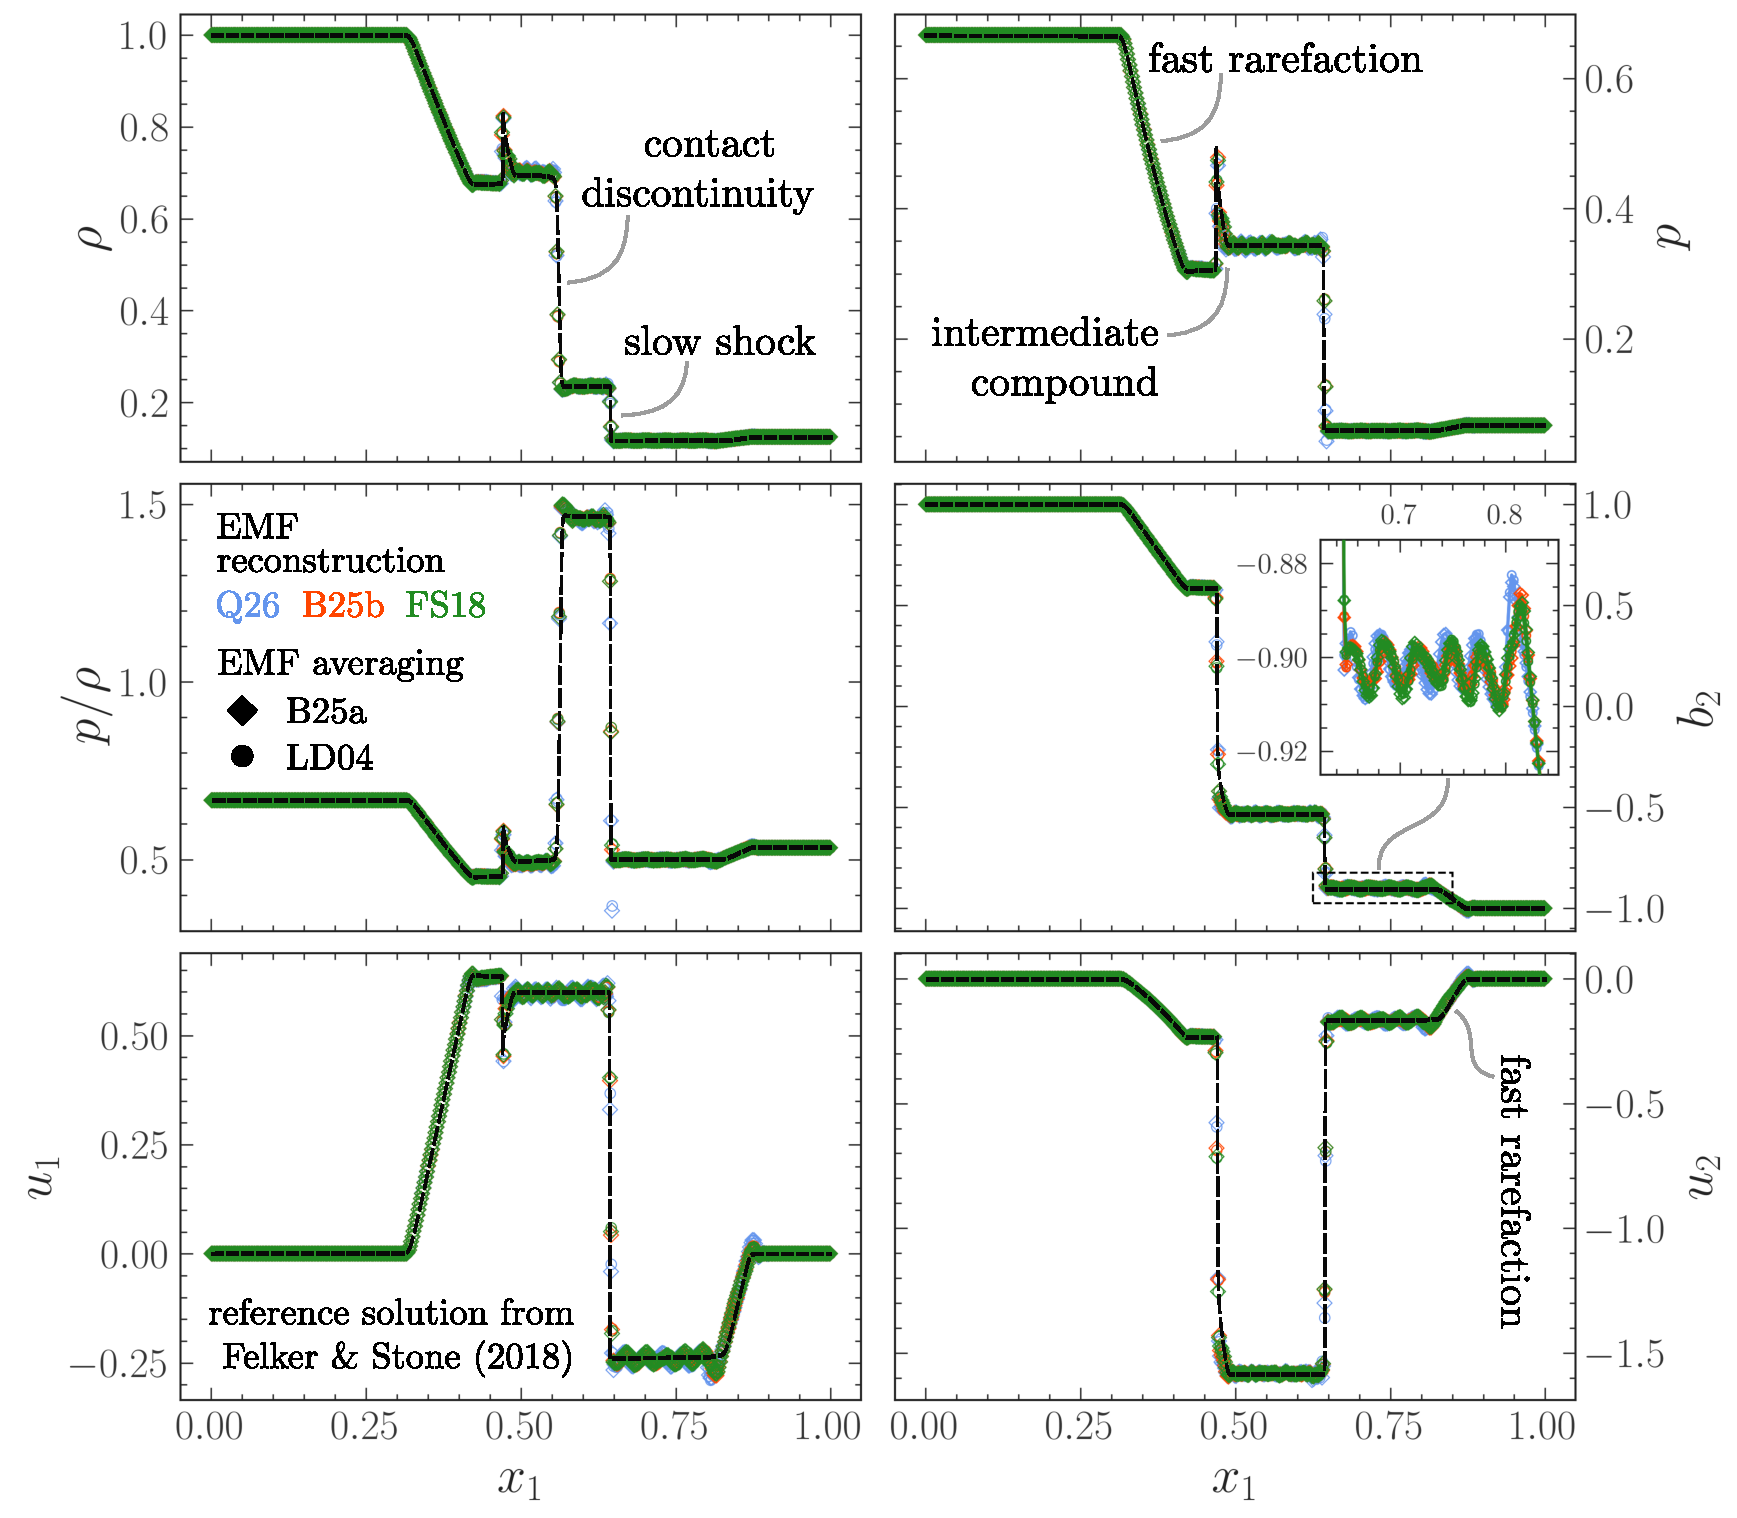
\includegraphics[width=\linewidth]{figures/quokka-mhd/results/bw-profiles.pdf}
%DIFDELCMD <     %%%
%DIFDELCMD < \caption{%
{%DIFAUXCMD
\DIFdelFL{Results for the \mbox{%DIFAUXCMD
\citet{Brio88a} }\hskip0pt%DIFAUXCMD
shock tube test. The panels show, from top left and proceeding across and down, density, pressure, ratio of pressure to density, magnetic field in the $x_2$ direction, and velocity in the $x_1$ and $x_2$ directions. Solutions generated using Q26, \mbox{%DIFAUXCMD
\citetalias{Balsara25a}}\hskip0pt%DIFAUXCMD
, and \mbox{%DIFAUXCMD
\citetalias{Felker18a} }\hskip0pt%DIFAUXCMD
EMF reconstruction are shown in blue, red, and green, respectively, while those using \mbox{%DIFAUXCMD
\citetalias{Balsara25b} }\hskip0pt%DIFAUXCMD
and \mbox{%DIFAUXCMD
\citetalias{Londrillo04a} }\hskip0pt%DIFAUXCMD
EMF averaging are shown by diamond and circular symbols, respectively. The dashed black line show the reference solution, which we take from \mbox{%DIFAUXCMD
\citetalias{Felker18a}}\hskip0pt%DIFAUXCMD
. Annotations indicate the different discontinuities in the solution.}}
    %DIFAUXCMD
%DIFDELCMD < \label{fig:bw-profiles}
%DIFDELCMD < \end{figure}
%DIFDELCMD < %%%
\DIFdelend \DIFaddbegin \subsection{\DIFadd{Resolving turbulent structures}}
\label{sec:scheme-comparison:orszag-tang}
\DIFaddend

\DIFdelbegin \subsection{\DIFdel{Stability and accuracy for non-linear problems}}
%DIFAUXCMD
\addtocounter{subsection}{-1}%DIFAUXCMD
%DIFDELCMD < \label{sec:performance:orszag-tang}
%DIFDELCMD < %%%
\DIFdelend \DIFaddbegin \subsubsection{\DIFadd{The Orszag-Tang vortex}}
\label{sec:scheme-comparison:orszag-tang:setup}
\DIFaddend

\DIFdelbegin \DIFdel{To test the stability }\DIFdelend \DIFaddbegin \DIFadd{We next test each }\DIFaddend of our scheme combinations \DIFdelbegin \DIFdel{, we use }\DIFdelend \DIFaddbegin \DIFadd{on }\DIFaddend the Orszag-Tang \DIFdelbegin \DIFdel{test \mbox{%DIFAUXCMD
\citep{OrszagTang1979}}\hskip0pt%DIFAUXCMD
. This is a two-dimensional }\DIFdelend \DIFaddbegin \DIFadd{vortex \mbox{%DIFAUXCMD
\citep{OrszagTang1979}}\hskip0pt%DIFAUXCMD
, a 2D }\DIFaddend non-linear MHD \DIFdelbegin \DIFdel{vortex that evolves }\DIFdelend \DIFaddbegin \DIFadd{problem that evolves an initially smooth vortex, threaded by a magnetic field, }\DIFaddend into interacting shocks and current sheets\DIFdelbegin \DIFdel{and tests the Riemann solverand the EMF reconstruction schemes. We run all tests at a high resolution of $1024\times 1024 \times 8$ and to time $t=1$, long enough for the system to mix and develop interacting shock waves, in order to test the robustness of the schemes in a high-stress problem.
All our tests for this section use eight GPUs.
}\DIFdelend \DIFaddbegin \DIFadd{. We simulate this flow with $\gamma = 5/3$, on a domain $x_0, x_1 \in [-0.5, 0.5]$, initialised such that
}\begin{align}
    \rho(\mVector{x})
        &= \frac{25}{36\pi} \\
    \mVector{u}(\mVector{x})
        &= \sin\sbrac{2\pi x_1}\, \mVectorUnit{x}_0
        - \sin\sbrac{2\pi x_0}\, \mVectorUnit{x}_1 \\
    p(\mVector{x})
        &= \frac{5}{12\pi} \\
    \mVector{b}(\mVector{x})
        &= \frac{1}{\sqrt{4\pi}} \sin\sbrac{2\pi x_1}\, \mVectorUnit{x}_0
        + \frac{1}{\sqrt{4\pi}} \sin\sbrac{4\pi x_0}\, \mVectorUnit{x}_1
    .
\end{align}
\DIFadd{This test is widely used to exercise all aspects of an MHD solver, so we use it as a stress test of every scheme combination (EMF compute, EMF averaging, and reconstruction scheme), run at a resolution of $1024^2$. We also compare PPM and PPM-EP reconstruction at $4096^2$, run with Q26 compute and \mbox{%DIFAUXCMD
\citetalias{Balsara25b} }\hskip0pt%DIFAUXCMD
averaging, to confirm our conclusions about PPM-clipping hold at higher resolution.
}\DIFaddend

\DIFaddbegin \DIFadd{In this test, the first series of shocks collide at around $t \approx 0.5$, with mixing and shock generation peaking around $t \approx 0.85$; we therefore run every simulation to $t = 1$, to confirm that it completes without failure, and then compare all schemes at $t = 0.85$.
}

\subsubsection{\DIFadd{Analysis of resolved structures}}
\label{sec:scheme-comparison:orszag-tang:discussion}

\begin{figure*}
    \centering
    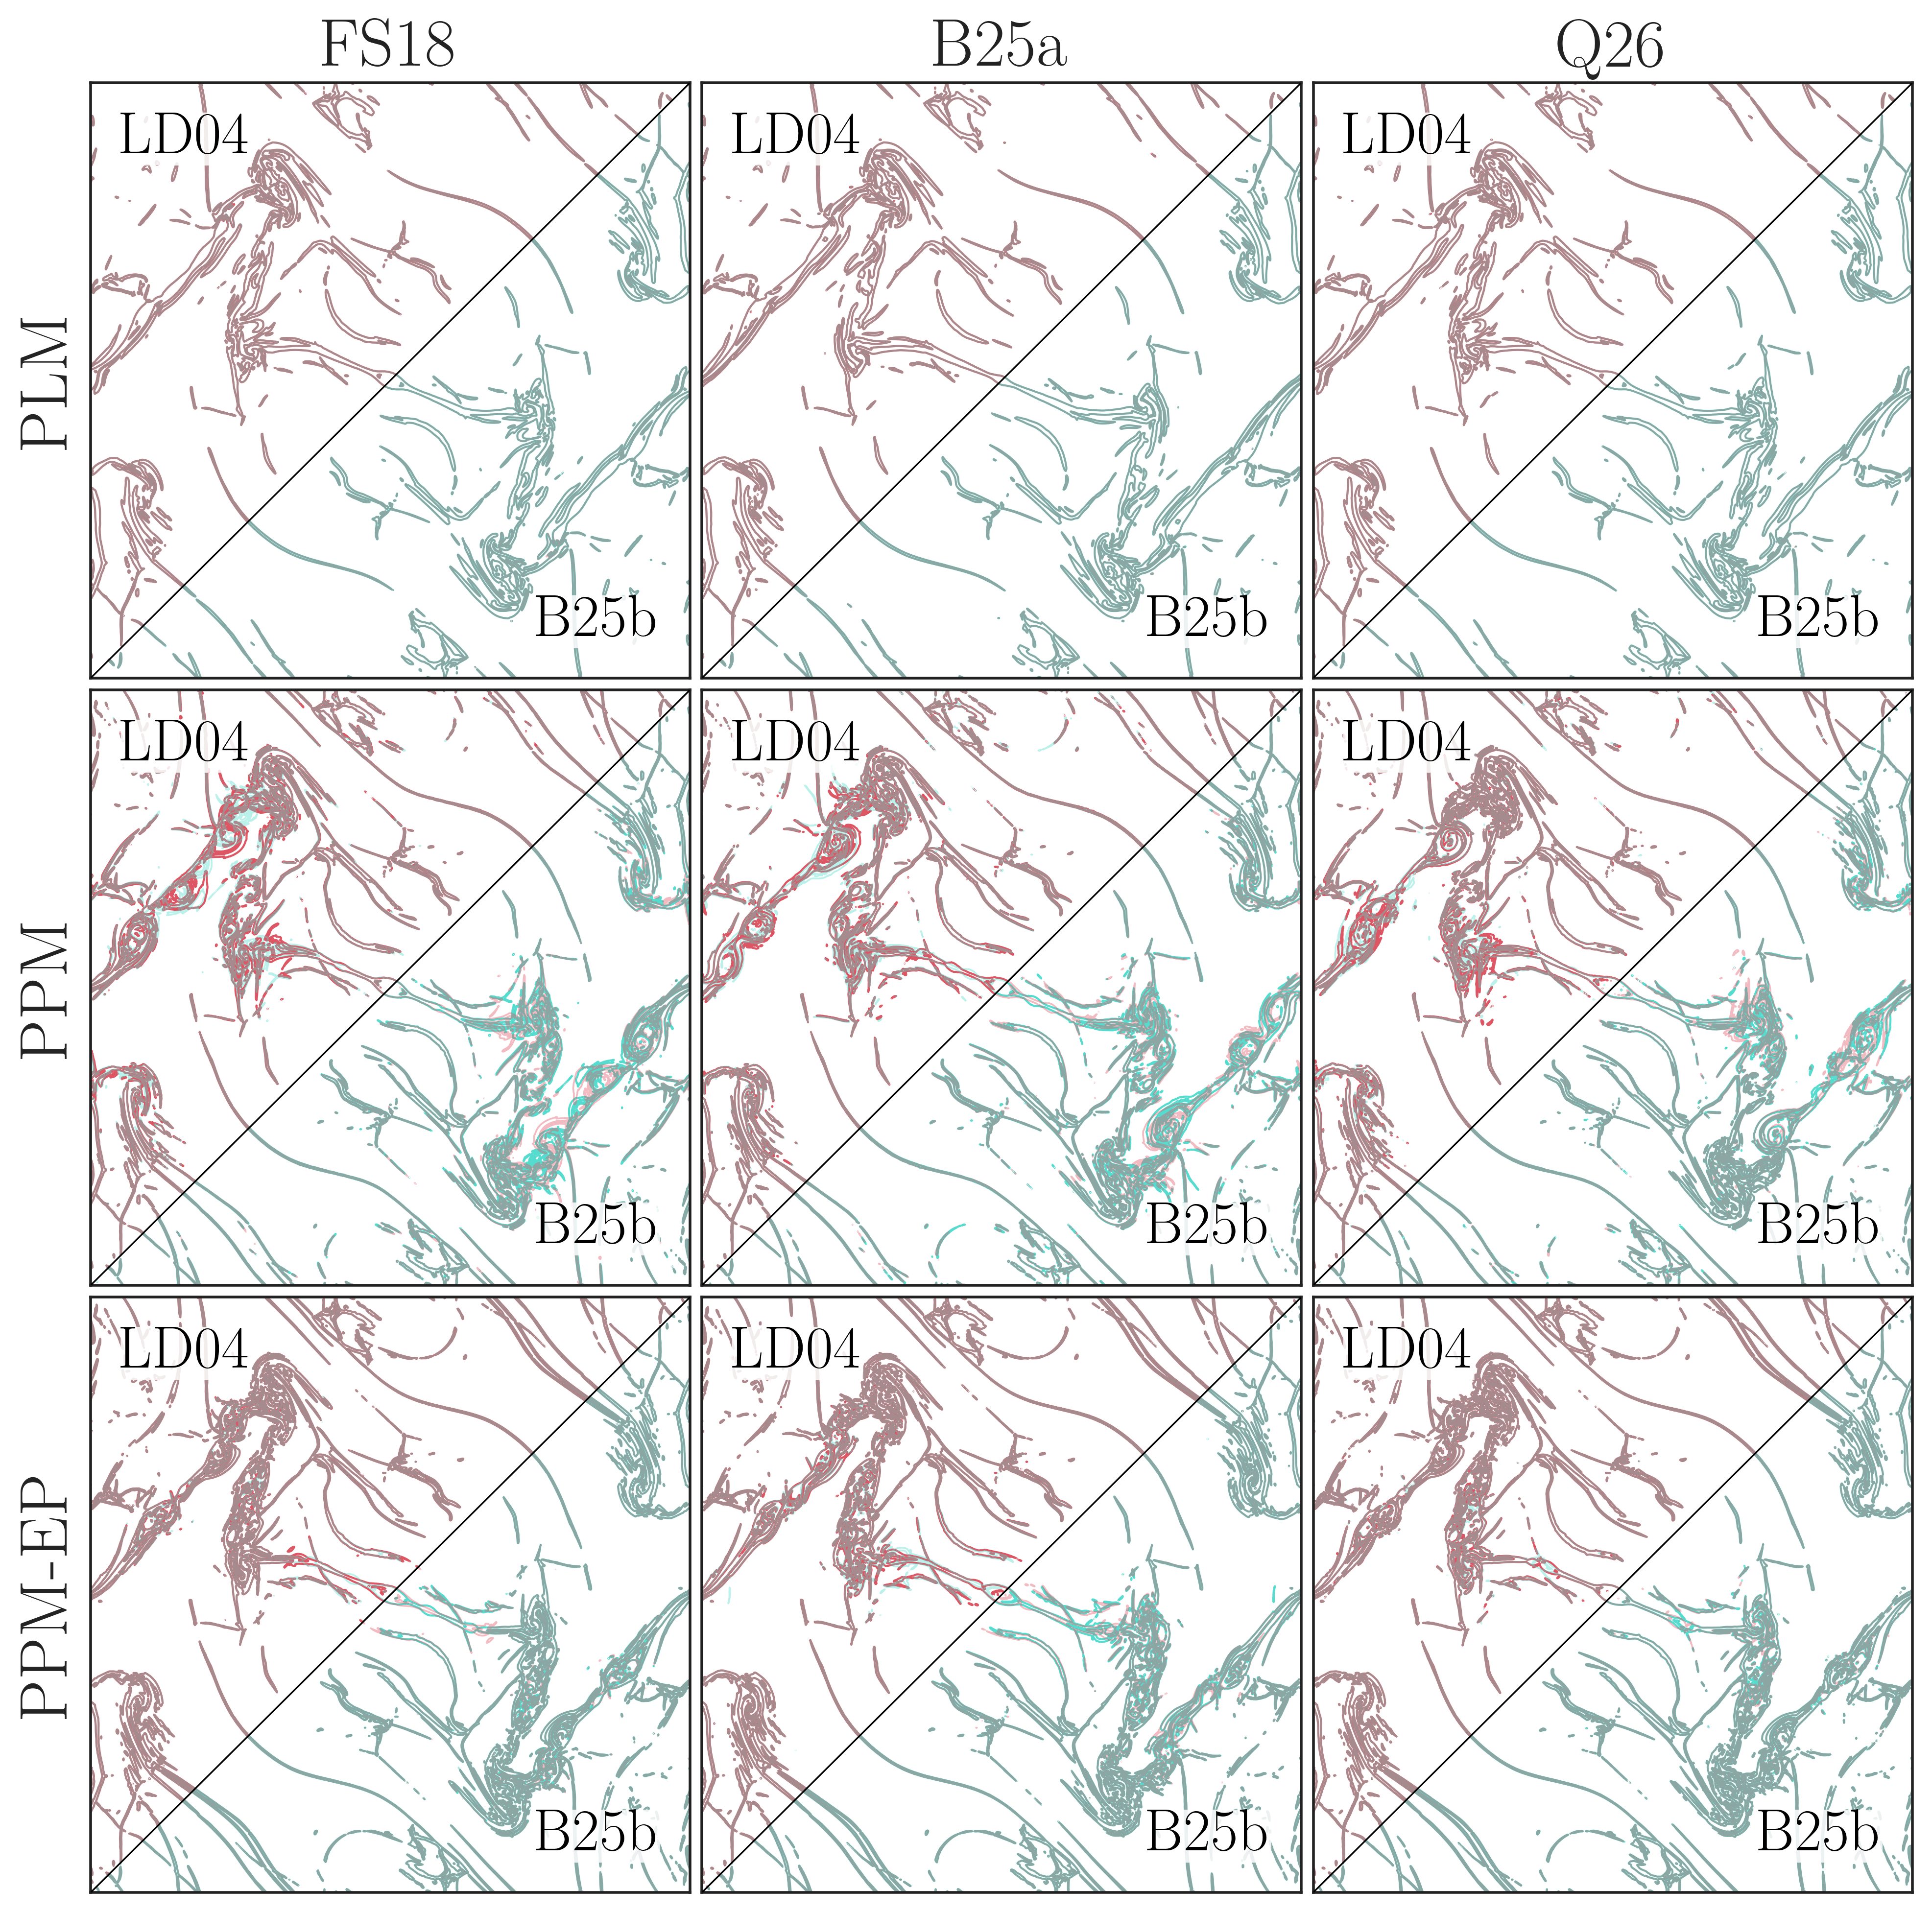
\includegraphics[width=\linewidth]{figures/quokka-mhd/results/orszag-tang-emf-scheme-comparison.png}
    \caption{\DIFaddFL{Comparison of all 18 scheme combinations for the Orszag-Tang vortex (\sref{sec:scheme-comparison:orszag-tang:setup}) run at $1024^2$: reconstruction varies across rows (\sref{sec:methods:flux}), EMF compute across columns (\sref{sec:methods:emf:compute}), and both EMF averaging schemes (\sref{sec:methods:emf:averaging}) are compared in each panel. In each panel we compare snapshots at $t = 0.85$ of \mbox{%DIFAUXCMD
\citetalias{Londrillo04a} }\hskip0pt%DIFAUXCMD
(red) in the top-left corner and \mbox{%DIFAUXCMD
\citetalias{Balsara25b} }\hskip0pt%DIFAUXCMD
(blue) in the bottom-right corner, with contours tracing $\log_{10}\rbrac{\Delta x\, |\nabla\times\mVector{b}|} = -1.6$.}}
    \label{fig:orszag-tang:emf-schemes}
\end{figure*}

\DIFaddend \begin{figure}
    \centering
    \DIFdelbeginFL %DIFDELCMD < 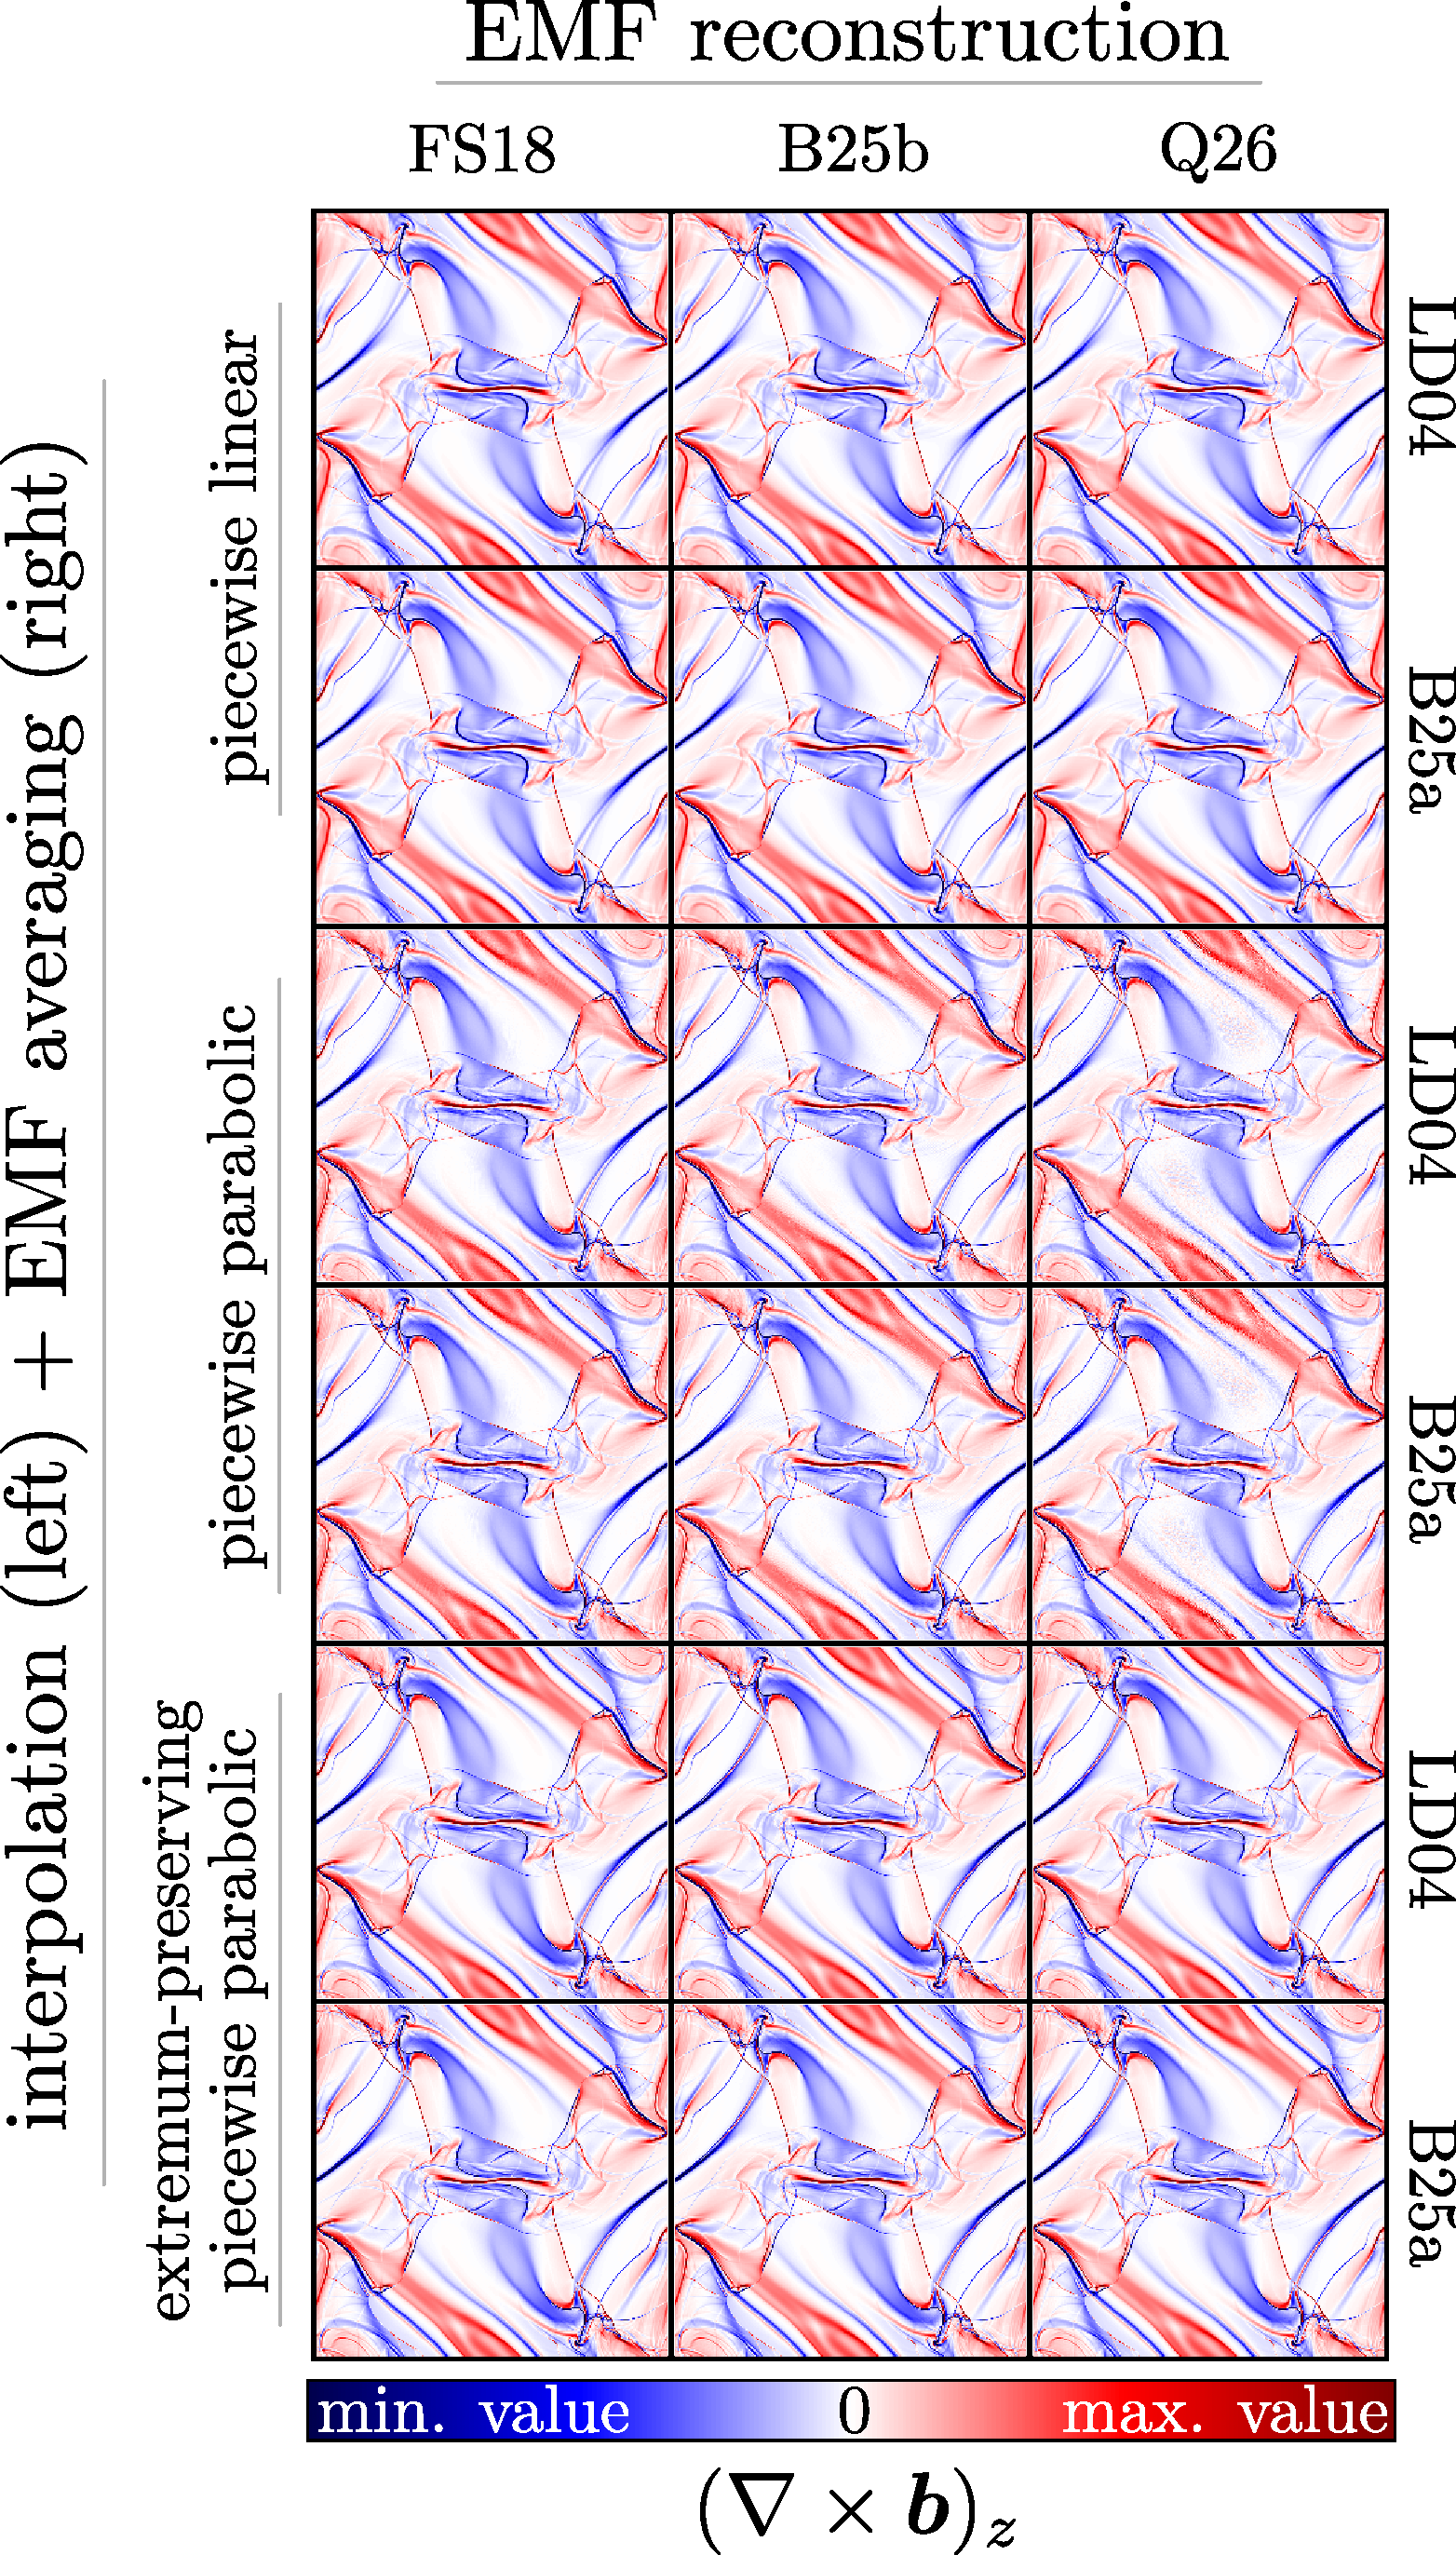
\includegraphics[width=0.75\linewidth]{figures/quokka-mhd/results/ot-schemes-lores.pdf}
%DIFDELCMD <     %%%
\DIFdelendFL \DIFaddbeginFL 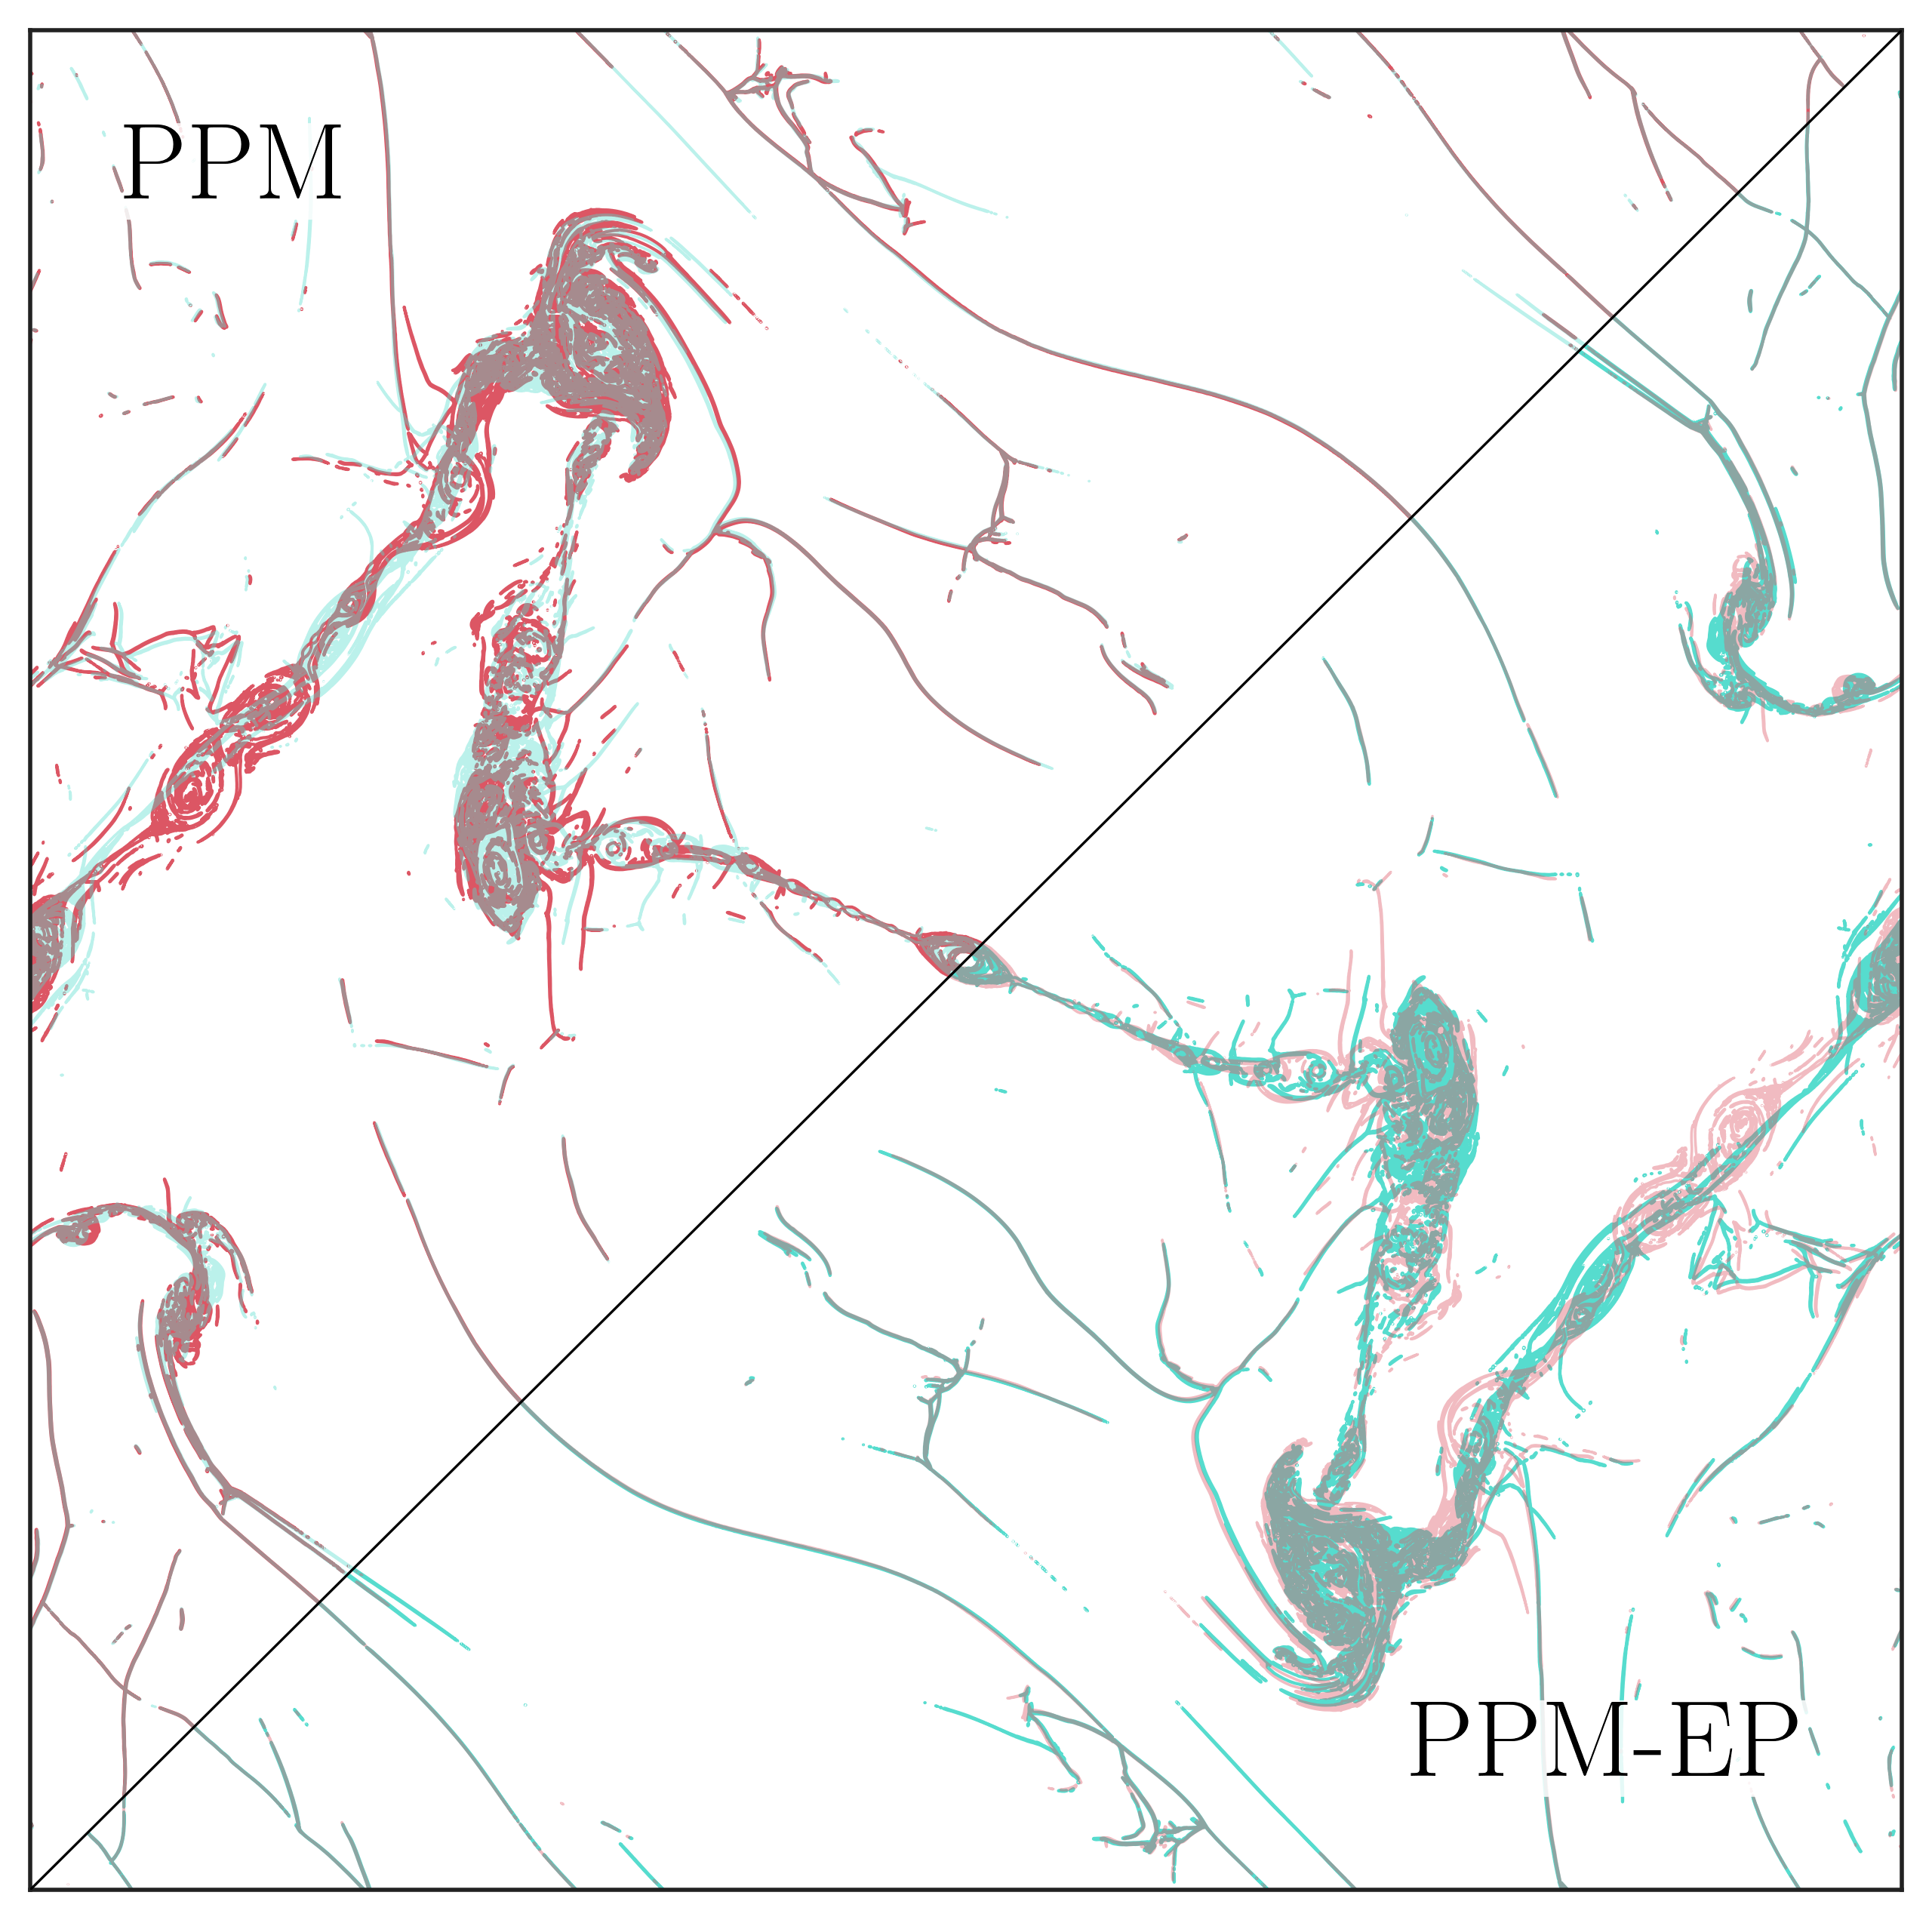
\includegraphics[width=0.65\linewidth]{figures/quokka-mhd/results/orszag-tang-reconstruction-scheme-comparison.png}
    \DIFaddendFL \caption{\DIFdelbeginFL \DIFdelFL{Slice plots taken through the midplane }\DIFdelendFL \DIFaddbeginFL \DIFaddFL{Comparison }\DIFaddendFL of \DIFdelbeginFL \DIFdelFL{the Orszag-Tang problem for each of combination of interpolation (labelled on the left)}\DIFdelendFL \DIFaddbeginFL \DIFaddFL{PPM and PPM-EP reconstruction}\DIFaddendFL , \DIFaddbeginFL \DIFaddFL{using our recommended }\DIFaddendFL EMF \DIFdelbeginFL \DIFdelFL{reconstruction }\DIFdelendFL \DIFaddbeginFL \DIFaddFL{combination }\DIFaddendFL (\DIFdelbeginFL \DIFdelFL{labelled on the top), }\DIFdelendFL \DIFaddbeginFL \DIFaddFL{Q26 compute }\DIFaddendFL and \DIFdelbeginFL \DIFdelFL{EMF }\DIFdelendFL \DIFaddbeginFL \DIFaddFL{\mbox{%DIFAUXCMD
\citetalias{Balsara25b} }\hskip0pt%DIFAUXCMD
}\DIFaddendFL averaging\DIFdelbeginFL \DIFdelFL{(labelled on the right}\DIFdelendFL )\DIFdelbeginFL \DIFdelFL{. The size of the computational domain shown is $1\times 1$ in dimensionless units}\DIFdelendFL , \DIFdelbeginFL \DIFdelFL{and we plot }\DIFdelendFL \DIFaddbeginFL \DIFaddFL{for }\DIFaddendFL the \DIFdelbeginFL \DIFdelFL{out-of-plane component of the current density }\DIFdelendFL \DIFaddbeginFL \DIFaddFL{Orszag-Tang vortex run }\DIFaddendFL at \DIFdelbeginFL \DIFdelFL{$t = 0.5$}\DIFdelendFL \DIFaddbeginFL \DIFaddFL{$4096^2$, following the same format as \mbox{%DIFAUXCMD
\cref{fig:orszag-tang:emf-schemes}}\hskip0pt%DIFAUXCMD
}\DIFaddendFL .}
    \DIFdelbeginFL %DIFDELCMD < \label{fig:OT_current}
%DIFDELCMD < %%%
\DIFdelendFL \DIFaddbeginFL \label{fig:orszag-tang:reconstruction-schemes}
\DIFaddendFL \end{figure}

\DIFdelbegin \DIFdel{We show the current density in the out-of-plane direction at $t=0.5$ that we obtain for this problem in }%DIFDELCMD < \autoref{fig:OT_current}%%%
\DIFdel{, for each combination of EMF reconstruction scheme}\DIFdelend \DIFaddbegin \DIFadd{In this section we exploit the fact that our implementation of our full suite of CT-MHD schemes (across Riemann solvers, EMF compute}\DIFaddend , EMF averaging\DIFdelbegin \DIFdel{scheme, and interpolation type that we tested. From this figure we can make a few observations. First, }\DIFdelend \DIFaddbegin \DIFadd{, and reconstruction order) preserves point-reflection symmetry to bit-level precision. Thus all differences between schemes we identify reflect differences in how each scheme combination resolves the flow, and not an artefact induced by numerical symmetry breaking. With this in mind, we compare two schemes by overlaying their resolved current-density structure at $t = 0.85$. We do this by drawing the contour $\log_{10}\rbrac{\Delta x\, |\nabla\times\mVector{b}|} = -1.6$ for both schemes on a panel, opaque in one half of the domain (split along the off-diagonal) and faint in the other; differences between }\DIFaddend the \DIFdelbegin \DIFdel{most obvious differences are between interpolation methods -- PLM (top two rows) versus PPM (middle two rows) versus PPM-EP (bottom two rows). The PLM results are noticeably smoother and less noisy, while the PPM and PPM-EP results both have some clear ringing, though more for PPM than PPM-EP. Second, the differences between EMF averaging method (\mbox{%DIFAUXCMD
\citetalias{Londrillo04a} }\hskip0pt%DIFAUXCMD
versus \mbox{%DIFAUXCMD
\citetalias{Balsara25b}}\hskip0pt%DIFAUXCMD
) are minimal -- the first and second rows are nearly identical, as are the third and fourth, and fifth and sixth. Finally, the choice of EMF reconstruction method (\mbox{%DIFAUXCMD
\citetalias{Felker18a} }\hskip0pt%DIFAUXCMD
versus \mbox{%DIFAUXCMD
\citetalias{Balsara25a} }\hskip0pt%DIFAUXCMD
versus Q26) makes almost no difference with PLM interpolation (top two rows), and does not change the large scale characteristics of the solution with }\DIFdelend \DIFaddbegin \DIFadd{two schemes are then highlighted by regions where both colours are visible. That is, if two schemes produced exactly identical results we would see only one colour on each side of the diagonal, so any deviation from this is evidence of differences between the schemes.
}

\DIFadd{\mbox{%DIFAUXCMD
\Cref{fig:orszag-tang:emf-schemes} }\hskip0pt%DIFAUXCMD
uses this plotting technique to compare all 18 scheme combinations run at $1024^2$, arranged in a $3\times 3$ grid, with EMF compute scheme varying across columns, reconstruction order across rows, and EMF averaging scheme within each panel. Across all these comparisons, the schemes broadly resolve the same underlying structures, with the clearest differences arising from reconstruction order: PLM resolves substantially less turbulent structure than either }\DIFaddend PPM or PPM-EP, \DIFdelbegin \DIFdel{but does make a difference to the pattern of ringing with these higher-order methods. For example, with PPM interpolation (middle two rows), the \mbox{%DIFAUXCMD
\citetalias{Felker18a} }\hskip0pt%DIFAUXCMD
method (left column) shows less ringing than \mbox{%DIFAUXCMD
\citetalias{Balsara25a}}\hskip0pt%DIFAUXCMD
, which in turn shows less ringing than Q26, and in going between \mbox{%DIFAUXCMD
\citetalias{Balsara25a} }\hskip0pt%DIFAUXCMD
and Q26 (middle and right columns) the orientation of the ringing pattern rotates by $\approx 90^\circ$}\DIFdelend \DIFaddbegin \DIFadd{regardless of the EMF scheme combination. This mirrors the wave-convergence results (\sref{sec:scheme-comparison:waves}), where PLM required roughly $4\times$ higher resolution to achieve the same accuracy as PPM-EP}\DIFaddend .

\DIFdelbegin %DIFDELCMD < \begin{table}
%DIFDELCMD < \centering
%DIFDELCMD < %%%
%DIFDELCMD < \caption{%
{%DIFAUXCMD
\DIFdelFL{Number of time steps required to reach $t=1$ (third column) and number of first-order flux corrections (right column) for the Orszag-Tang test using different schemes for interpolation, EMF reconstruction (first column), and averaging (second column).
}%DIFDELCMD < \label{tab:ot_steps}
%DIFDELCMD < %%%
}
%DIFAUXCMD
%DIFDELCMD < \begin{tabular}{llcr}
%DIFDELCMD < \hline\hline
%DIFDELCMD < %%%
\DIFdelFL{Reconstruction }%DIFDELCMD < & %%%
\DIFdelFL{Averaging }%DIFDELCMD < & %%%
\DIFdelFL{N. time steps }%DIFDELCMD < & %%%
\DIFdelFL{N. FOFC steps  }%DIFDELCMD < \\
%DIFDELCMD < \hline
%DIFDELCMD < %%%
%DIFDELCMD < \multicolumn{4}{c}{%
{%DIFAUXCMD
\DIFdelFL{PLM interpolation}} %DIFAUXCMD
%DIFDELCMD < \\
%DIFDELCMD < \hline
%DIFDELCMD < %%%
\DIFdelFL{FS18 }%DIFDELCMD < & %%%
\DIFdelFL{LD04  }%DIFDELCMD < &  %%%
\DIFdelFL{15985 }%DIFDELCMD < & %%%
\DIFdelFL{0 }%DIFDELCMD < \\
%DIFDELCMD < %%%
\DIFdelFL{FS18 }%DIFDELCMD < & %%%
\DIFdelFL{B25a  }%DIFDELCMD < &  %%%
\DIFdelFL{15989 }%DIFDELCMD < & %%%
\DIFdelFL{0 }%DIFDELCMD < \\
%DIFDELCMD < %%%
\DIFdelFL{B25b }%DIFDELCMD < & %%%
\DIFdelFL{LD04  }%DIFDELCMD < &  %%%
\DIFdelFL{16005 }%DIFDELCMD < & %%%
\DIFdelFL{0 }%DIFDELCMD < \\
%DIFDELCMD < %%%
\DIFdelFL{B25b }%DIFDELCMD < & %%%
\DIFdelFL{B25a  }%DIFDELCMD < &  %%%
\DIFdelFL{15948 }%DIFDELCMD < & %%%
\DIFdelFL{0 }%DIFDELCMD < \\
%DIFDELCMD < %%%
\DIFdelFL{Q26  }%DIFDELCMD < & %%%
\DIFdelFL{LD04  }%DIFDELCMD < & %%%
\DIFdelFL{18335 }%DIFDELCMD < & %%%
\DIFdelFL{0 }%DIFDELCMD < \\
%DIFDELCMD < %%%
\DIFdelFL{Q26  }%DIFDELCMD < & %%%
\DIFdelFL{B25a  }%DIFDELCMD < &  %%%
\DIFdelFL{19339 }%DIFDELCMD < & %%%
\DIFdelFL{0 }%DIFDELCMD < \\
%DIFDELCMD < \hline
%DIFDELCMD < %%%
%DIFDELCMD < \multicolumn{4}{c}{%
{%DIFAUXCMD
\DIFdelFL{PPM interpolation}} %DIFAUXCMD
%DIFDELCMD < \\
%DIFDELCMD < \hline
%DIFDELCMD < %%%
\DIFdelFL{FS18 }%DIFDELCMD < & %%%
\DIFdelFL{LD04  }%DIFDELCMD < &  %%%
\DIFdelFL{16149 }%DIFDELCMD < & %%%
\DIFdelFL{0 }%DIFDELCMD < \\
%DIFDELCMD < %%%
\DIFdelFL{FS18 }%DIFDELCMD < & %%%
\DIFdelFL{B25a  }%DIFDELCMD < &  %%%
\DIFdelFL{16153 }%DIFDELCMD < & %%%
\DIFdelFL{0 }%DIFDELCMD < \\
%DIFDELCMD < %%%
\DIFdelFL{B25b }%DIFDELCMD < & %%%
\DIFdelFL{LD04  }%DIFDELCMD < &  %%%
\DIFdelFL{16210 }%DIFDELCMD < & %%%
\DIFdelFL{0 }%DIFDELCMD < \\
%DIFDELCMD < %%%
\DIFdelFL{B25b }%DIFDELCMD < & %%%
\DIFdelFL{B25a  }%DIFDELCMD < &  %%%
\DIFdelFL{16282 }%DIFDELCMD < & %%%
\DIFdelFL{0 }%DIFDELCMD < \\
%DIFDELCMD < %%%
\DIFdelFL{Q26  }%DIFDELCMD < & %%%
\DIFdelFL{LD04  }%DIFDELCMD < &   %%%
\DIFdelFL{41231 }%DIFDELCMD < & %%%
\DIFdelFL{0 }%DIFDELCMD < \\
%DIFDELCMD < %%%
\DIFdelFL{Q26  }%DIFDELCMD < & %%%
\DIFdelFL{B25a  }%DIFDELCMD < &  %%%
\DIFdelFL{\,$^{\dagger}$ }%DIFDELCMD < & %%%
\DIFdelFL{0 }%DIFDELCMD < \\
%DIFDELCMD < \hline
%DIFDELCMD < %%%
%DIFDELCMD < \multicolumn{4}{c}{%
{%DIFAUXCMD
\DIFdelFL{PPM-EP interpolation}} %DIFAUXCMD
%DIFDELCMD < \\
%DIFDELCMD < \hline
%DIFDELCMD < %%%
\DIFdelFL{FS18 }%DIFDELCMD < & %%%
\DIFdelFL{LD04  }%DIFDELCMD < &  %%%
\DIFdelFL{16295 }%DIFDELCMD < & %%%
\DIFdelFL{0 }%DIFDELCMD < \\
%DIFDELCMD < %%%
\DIFdelFL{FS18 }%DIFDELCMD < & %%%
\DIFdelFL{B25a  }%DIFDELCMD < &  %%%
\DIFdelFL{16286 }%DIFDELCMD < & %%%
\DIFdelFL{0 }%DIFDELCMD < \\
%DIFDELCMD < %%%
\DIFdelFL{B25b }%DIFDELCMD < & %%%
\DIFdelFL{LD04  }%DIFDELCMD < &  %%%
\DIFdelFL{16483 }%DIFDELCMD < & %%%
\DIFdelFL{0 }%DIFDELCMD < \\
%DIFDELCMD < %%%
\DIFdelFL{B25b }%DIFDELCMD < & %%%
\DIFdelFL{B25a  }%DIFDELCMD < &  %%%
\DIFdelFL{16527 }%DIFDELCMD < & %%%
\DIFdelFL{0 }%DIFDELCMD < \\
%DIFDELCMD < %%%
\DIFdelFL{Q26  }%DIFDELCMD < & %%%
\DIFdelFL{LD04  }%DIFDELCMD < & %%%
\DIFdelFL{\,$^{\ddagger}$ }%DIFDELCMD < & %%%
\DIFdelFL{80 }%DIFDELCMD < \\
%DIFDELCMD < %%%
\DIFdelFL{Q26  }%DIFDELCMD < & %%%
\DIFdelFL{B25a  }%DIFDELCMD < & %%%
\DIFdelFL{\,$^{\ddagger}$ }%DIFDELCMD < & %%%
\DIFdelFL{80 }%DIFDELCMD < \\
%DIFDELCMD < \hline\hline
%DIFDELCMD < \end{tabular}
%DIFDELCMD < \vspace{0.5ex}
%DIFDELCMD < \begin{flushleft}
%DIFDELCMD < \footnotesize
%DIFDELCMD < %%%
\DIFdelFL{$^{\dagger}$~Run terminated early because the time step became prohibitively small .}%DIFDELCMD < \\
%DIFDELCMD < %%%
\DIFdelFL{$^{\ddagger}$~Run became numerically unstable and crashed before reaching the final time.
}%DIFDELCMD < \end{flushleft}
%DIFDELCMD < \end{table}
%DIFDELCMD < %%%
\DIFdelend \DIFaddbegin \DIFadd{In contrast to \sref{sec:scheme-comparison:waves}, the differences here between PPM and PPM-EP are much smaller: both reconstruction schemes resolve the same level of structure across every EMF scheme combination. At $1024^2$, however, the flow remains in a dissipation-regulated regime: the effective Lundquist number, $c_\mathrm{A}L/\eta$ (where $\eta$ is the effective resistivity set by the resolution and EMF scheme), is too small for current sheets to fragment into plasmoid chains, so sheets instead remain laminar \mbox{%DIFAUXCMD
\citep{Landi15a}}\hskip0pt%DIFAUXCMD
. We therefore repeat this comparison at $4096^2$ in \mbox{%DIFAUXCMD
\cref{fig:orszag-tang:reconstruction-schemes}}\hskip0pt%DIFAUXCMD
, where, in both solutions, the lower effective numerical dissipation allows thin current sheets along the vortex arms to become tearing unstable and fragment into plasmoids. These plasmoids are advected along the current sheets, with some coalescing into larger magnetic islands; the precise locations of these islands at $t = 0.85$ differ between the two solutions.
}\DIFaddend

These differences in \DIFdelbegin \DIFdel{the amount of ringing manifest at later times as differences in stability. While all schemes run successfully up to the time shown in }%DIFDELCMD < \autoref{fig:OT_current}%%%
\DIFdel{, not all of them are able to continue up to $t=1$, or require the same number of time steps to reach this point.
We report in }%DIFDELCMD < \autoref{tab:ot_steps} %%%
\DIFdel{the number of time steps that each scheme required to reach $t=1$ and the number of first-order flux corrections that occurred; single and double daggers indicate that a given scheme terminated before reaching $t=1$ because the time step became prohibitively small or because the scheme crashed, respectively.
We see that the Q26 scheme behaves comparably to the others for PLM, albeit requiring slightly more time steps, but that it either requires many more time steps or fails altogether for the higher-order interpolation methods.
By contrast, the results for the \mbox{%DIFAUXCMD
\citetalias{Felker18a} }\hskip0pt%DIFAUXCMD
and \mbox{%DIFAUXCMD
\citetalias{Balsara25a} }\hskip0pt%DIFAUXCMD
reconstruction schemes,
and for both \mbox{%DIFAUXCMD
\citetalias{Londrillo04a} }\hskip0pt%DIFAUXCMD
and \mbox{%DIFAUXCMD
\citetalias{Balsara25b} }\hskip0pt%DIFAUXCMD
averaging , are nearly identical.
Thus the Q26 scheme provides comparable quality results to the others, but appears slightly less table at high order}\DIFdelend \DIFaddbegin \DIFadd{placement, however, do not provide a measure of relative accuracy: as \mbox{%DIFAUXCMD
\citet{Lecoanet16a} }\hskip0pt%DIFAUXCMD
demonstrate for the Kelvin-Helmholtz instability, without explicit dissipation, this class of problem (where secondary instabilities are present) has no unique solution as the resolution or numerical scheme changes. The relevant comparison is therefore not the placement of individual plasmoids, but instead whether both schemes recover the same tearing-mediated dynamics: since both do, PPM performs as well as PPM-EP here despite its clipping-induced dissipation.
}

\DIFadd{Finally, among the three EMF compute schemes and two EMF averaging schemes tested here, we find no systematic change in the structures that are resolved in \mbox{%DIFAUXCMD
\cref{fig:orszag-tang:emf-schemes}}\hskip0pt%DIFAUXCMD
. Therefore, even in a demanding non-linear problem like the Orszag-Tang vortex, all six EMF scheme combinations produce comparable results, and so we turn next to numerical stability, and then computational performance, to distinguish between these schemes.
}

\subsection{\DIFadd{Stability under tearing-mediated reconnection}}
\label{sec:scheme-comparison:reconnection}

\DIFadd{Unlike the previous tests that compared the accuracy and resolved structure across different scheme combinations, here we instead test their numerical stability using the \mbox{%DIFAUXCMD
\citet{HawleyStone95a} }\hskip0pt%DIFAUXCMD
and \mbox{%DIFAUXCMD
\citet{Stone08a} }\hskip0pt%DIFAUXCMD
current sheet problem. This test features a strong magnetic field reversal that, when evolved for a long time in low-dissipation flows, grows tearing unstable and produces increasingly larger plasmoids.
}

\DIFadd{We set this test up with $\gamma = 5/3$, and a background state where the magnetic field reverses direction across the domain,
}\begin{align}
    \mVector{S}_\mathrm{c}^{[\mathrm{bg}]}
        = \begin{Bmatrix}
                \rho \\
                \mVector{u} \\
                \mVector{b} \\
                e_\mathrm{tot}
            \end{Bmatrix}
        = \begin{Bmatrix}
                1 \\
                \mVector{0} \\
                b_\mathrm{bg} \, \mathrm{sgn}\sbrac{|x_0| - 0.25} \, \mVectorUnit{x}_1 \\
                \dfrac{p_\mathrm{bg}}{\gamma-1} + \dfrac{b_\mathrm{bg}^2}{2}
            \end{Bmatrix}
    ,
\end{align}
\DIFadd{where $b_\mathrm{bg} = 1$ and $p_\mathrm{bg} = 0.05$; these states are perturbed with,
}\begin{align}
    \mVector{S}_\mathrm{c}^{[\delta]}
        = \begin{Bmatrix}
                \delta\rho \\
                \delta \mVector{u} \\
                \delta \mVector{b} \\
                \delta e_\mathrm{tot}
            \end{Bmatrix}
        = \begin{Bmatrix}
                0 \\
                \delta u \sin\sbrac{2\pi x_1} \, \mVectorUnit{x}_0 \\
                \mVector{0} \\
                \dfrac{1}{2} (\delta u)^2 \sin^2\sbrac{2\pi x_1}
            \end{Bmatrix},
\end{align}
\DIFadd{and $\delta u = 0.1$. We run this at $1024^2$ through to $t = 10$ for all six EMF compute and averaging scheme combinations, coupled with both PPM and PPM-EP reconstruction.
}

\DIFadd{Since we run without explicit resistivity, reconnection is entirely mediated by numerical dissipation, which, at this moderately-high resolution, allows sharp gradients to form around tearing unstable regions. After many small plasmoids have formed, they quickly merge in succession to form larger plasmoids, where each merger produces even sharper, transient gradients in regions of reconnecting plasmoids. This early period ($t \lesssim 1$) of the problem}\footnote{
    \DIFadd{We show the full time evolution of this problem in \sref{sec:stress-tests:current-sheet}.
}} \DIFadd{is the most numerically demanding part, yet we find that all scheme combinations run with plain PPM reconstruction resolve these plasmoid mergers stably all the way through to $t = 10$. With PPM-EP, however, we find that only two scheme combinations complete successfully: Q26 with \mbox{%DIFAUXCMD
\citetalias{Balsara25b}}\hskip0pt%DIFAUXCMD
, and \mbox{%DIFAUXCMD
\citetalias{Balsara25a} }\hskip0pt%DIFAUXCMD
with \mbox{%DIFAUXCMD
\citetalias{Balsara25b}}\hskip0pt%DIFAUXCMD
; every other scheme combination becomes numerically unstable during early plasmoid growth ($t < 1$)}\DIFaddend .

\subsection{Performance and scaling}
\DIFdelbegin %DIFDELCMD < \label{sec:performance:speed}
%DIFDELCMD < %%%
\DIFdelend \DIFaddbegin \label{sec:scheme-comparison:speed}
\DIFaddend

\DIFdelbegin %DIFDELCMD < \begin{table}
%DIFDELCMD < %%%
\DIFdelendFL \DIFaddbeginFL \begin{figure*}
    \DIFaddendFL \centering
    \DIFaddbeginFL 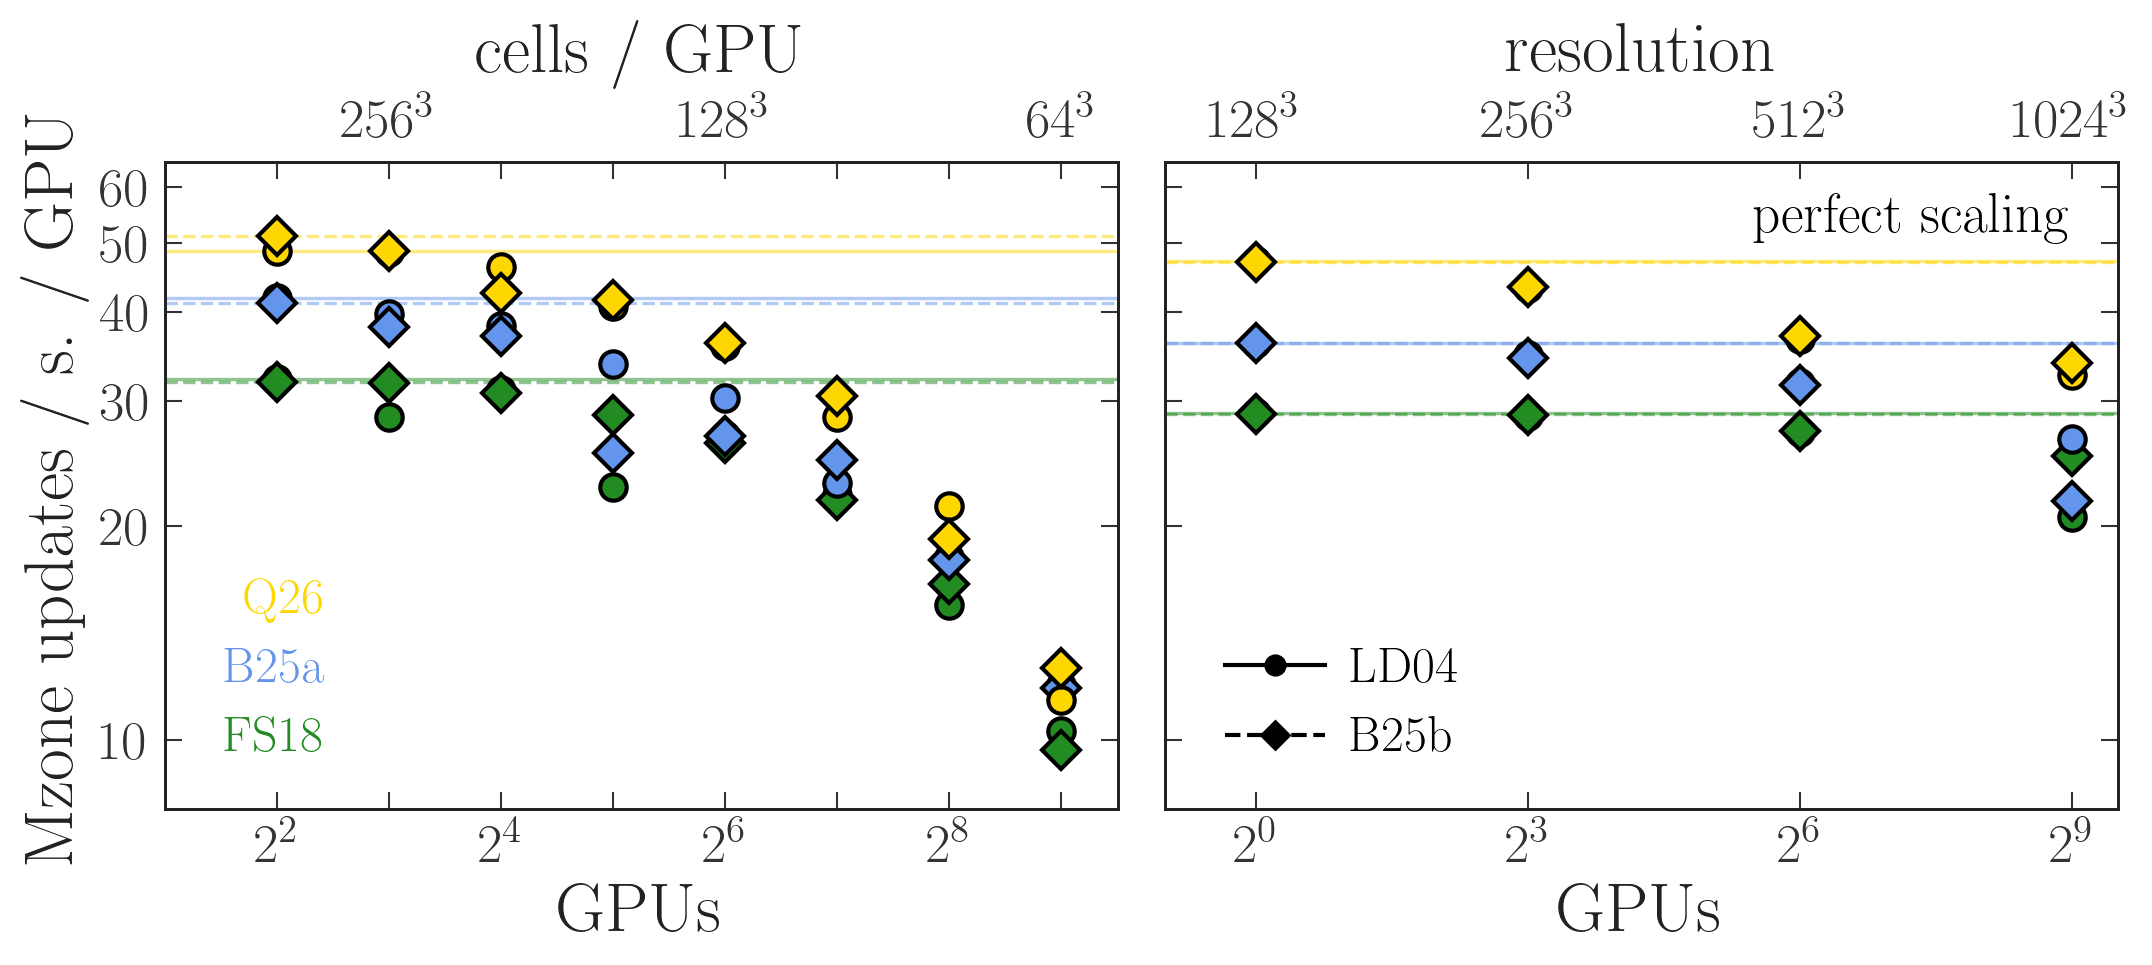
\includegraphics[width=\linewidth]{figures/quokka-mhd/results/performance-gpu-scaling.png}
    \DIFaddendFL \caption{\DIFdelbeginFL \DIFdelFL{Weak scaling test results }\DIFdelendFL \DIFaddbeginFL \DIFaddFL{Comparison of 6 EMF scheme combinations }\DIFaddendFL for \DIFdelbeginFL \DIFdelFL{different schemes and }\DIFdelendFL GPU \DIFdelbeginFL \DIFdelFL{counts in a test }\DIFdelendFL \DIFaddbeginFL \DIFaddFL{throughput and scaling (\sref{sec:scheme-comparison:speed}), all paired }\DIFaddendFL with \DIFdelbeginFL \DIFdelFL{$128^3$ cells per GPU. The first two columns indicate the EMF }\DIFdelendFL \DIFaddbeginFL \DIFaddFL{PPM-EP }\DIFaddendFL reconstruction\DIFaddbeginFL \DIFaddFL{: EMF compute (indicated by colour; \sref{sec:methods:emf:compute}) }\DIFaddendFL and \DIFaddbeginFL \DIFaddFL{EMF }\DIFaddendFL averaging \DIFdelbeginFL \DIFdelFL{schemes, and the remaining columns show results as a function of GPU count}\DIFdelendFL \DIFaddbeginFL \DIFaddFL{(indicated by marker; \sref{sec:methods:emf:averaging})}\DIFaddendFL . \DIFdelbeginFL \DIFdelFL{Entries in the remaining columns report the cell advance time $t_\mathrm{adv}$ in units of ns, defined as the amount of }\DIFdelendFL \DIFaddbeginFL \DIFaddFL{Cell updates per second per }\DIFaddendFL GPU \DIFdelbeginFL \DIFdelFL{time required to advance }\DIFdelendFL \DIFaddbeginFL \DIFaddFL{are shown for strong scaling at }\DIFaddendFL a \DIFdelbeginFL \DIFdelFL{single cell through one time step, }\DIFdelendFL \DIFaddbeginFL \DIFaddFL{fixed problem size of $512^3$ cells (left panel) }\DIFaddendFL and \DIFdelbeginFL \DIFdelFL{different }\DIFdelendFL \DIFaddbeginFL \DIFaddFL{weak scaling at $128^3$ cells per }\DIFaddendFL GPU \DIFdelbeginFL \DIFdelFL{counts $N_\mathrm{GPU}$}\DIFdelendFL \DIFaddbeginFL \DIFaddFL{(right panel); lines indicate perfect scaling for each scheme combination}\DIFaddendFL .}
    \DIFdelbeginFL %DIFDELCMD < \label{tab:weak_scaling_zone_update_times_ngpu}
%DIFDELCMD < \begin{tabular}{llrrrr}
%DIFDELCMD < \hline\hline
%DIFDELCMD < & & %%%
%DIFDELCMD < \multicolumn{4}{c}{%
{%DIFAUXCMD
\DIFdelFL{$t_\mathrm{adv}/\mathrm{ns}$ at $N_\mathrm{GPU}=\cdots$}} %DIFAUXCMD
%DIFDELCMD < \\
%DIFDELCMD < %%%
\DIFdelFL{Reconstruction }%DIFDELCMD < & %%%
\DIFdelFL{Averaging }%DIFDELCMD < & %%%
\DIFdelFL{1 }%DIFDELCMD < & %%%
\DIFdelFL{8 }%DIFDELCMD < & %%%
\DIFdelFL{64 }%DIFDELCMD < & %%%
\DIFdelFL{512 }%DIFDELCMD < \\
%DIFDELCMD < \hline
%DIFDELCMD < %%%
\DIFdelFL{FS18 }%DIFDELCMD < & %%%
\DIFdelFL{LD04  }%DIFDELCMD < & %%%
\DIFdelFL{34.65 }%DIFDELCMD < & %%%
\DIFdelFL{34.94 }%DIFDELCMD < & %%%
\DIFdelFL{36.84 }%DIFDELCMD < & %%%
\DIFdelFL{48.51 }%DIFDELCMD < \\
%DIFDELCMD < %%%
\DIFdelFL{FS18 }%DIFDELCMD < & %%%
\DIFdelFL{B25a  }%DIFDELCMD < & %%%
\DIFdelFL{34.76 }%DIFDELCMD < & %%%
\DIFdelFL{34.88 }%DIFDELCMD < & %%%
\DIFdelFL{36.74 }%DIFDELCMD < & %%%
\DIFdelFL{39.83 }%DIFDELCMD < \\
%DIFDELCMD < %%%
\DIFdelFL{B25b }%DIFDELCMD < & %%%
\DIFdelFL{LD04  }%DIFDELCMD < & %%%
\DIFdelFL{27.58 }%DIFDELCMD < & %%%
\DIFdelFL{28.71 }%DIFDELCMD < & %%%
\DIFdelFL{31.44 }%DIFDELCMD < & %%%
\DIFdelFL{37.69 }%DIFDELCMD < \\
%DIFDELCMD < %%%
\DIFdelFL{B25b }%DIFDELCMD < & %%%
\DIFdelFL{B25a  }%DIFDELCMD < & %%%
\DIFdelFL{27.65 }%DIFDELCMD < & %%%
\DIFdelFL{28.94 }%DIFDELCMD < & %%%
\DIFdelFL{31.58 }%DIFDELCMD < & %%%
\DIFdelFL{46.07 }%DIFDELCMD < \\
%DIFDELCMD < %%%
\DIFdelFL{Q26  }%DIFDELCMD < & %%%
\DIFdelFL{LD04  }%DIFDELCMD < & %%%
\DIFdelFL{21.19 }%DIFDELCMD < & %%%
\DIFdelFL{23.12 }%DIFDELCMD < & %%%
\DIFdelFL{27.24 }%DIFDELCMD < & %%%
\DIFdelFL{30.58 }%DIFDELCMD < \\
%DIFDELCMD < %%%
\DIFdelFL{Q26  }%DIFDELCMD < & %%%
\DIFdelFL{B25a  }%DIFDELCMD < & %%%
\DIFdelFL{21.23 }%DIFDELCMD < & %%%
\DIFdelFL{23.02 }%DIFDELCMD < & %%%
\DIFdelFL{27.01 }%DIFDELCMD < & %%%
\DIFdelFL{29.44 }%DIFDELCMD < \\
%DIFDELCMD < \hline\hline
%DIFDELCMD < \end{tabular}
%DIFDELCMD < \end{table}
%DIFDELCMD < \begin{table*}
%DIFDELCMD < \centering
%DIFDELCMD < %%%
%DIFDELCMD < \caption{%
{%DIFAUXCMD
\DIFdelFL{Same as }%DIFDELCMD < \autoref{tab:weak_scaling_zone_update_times_ngpu}%%%
\DIFdelFL{, but now showing the advance times measured for strong scaling in a test with a fixed $512^3$ cells.}}
%DIFAUXCMD
%DIFDELCMD < \label{tab:strong_scaling_zone_update_times_ngpu}
%DIFDELCMD < \begin{tabular}{llrrrrrrrr}
%DIFDELCMD < \hline\hline
%DIFDELCMD < & & %%%
%DIFDELCMD < \multicolumn{8}{c}{%
{%DIFAUXCMD
\DIFdelFL{$t_\mathrm{adv}/\mathrm{ns}$ at $N_\mathrm{GPU}=\cdots$}} %DIFAUXCMD
%DIFDELCMD < \\
%DIFDELCMD < %%%
\DIFdelFL{Recon. }%DIFDELCMD < & %%%
\DIFdelFL{Ave. }%DIFDELCMD < &
%DIFDELCMD < %%%
\DIFdelFL{4 }%DIFDELCMD < & %%%
\DIFdelFL{8 }%DIFDELCMD < & %%%
\DIFdelFL{16 }%DIFDELCMD < & %%%
\DIFdelFL{32 }%DIFDELCMD < & %%%
\DIFdelFL{64 }%DIFDELCMD < & %%%
\DIFdelFL{128 }%DIFDELCMD < & %%%
\DIFdelFL{256 }%DIFDELCMD < & %%%
\DIFdelFL{512 }%DIFDELCMD < \\
%DIFDELCMD < \hline
%DIFDELCMD < %%%
\DIFdelFL{FS18 }%DIFDELCMD < & %%%
\DIFdelFL{LD04
}%DIFDELCMD < & %%%
\DIFdelFL{31.03 }%DIFDELCMD < & %%%
\DIFdelFL{35.10 }%DIFDELCMD < & %%%
\DIFdelFL{32.16 }%DIFDELCMD < & %%%
\DIFdelFL{43.94 }%DIFDELCMD < & %%%
\DIFdelFL{37.22 }%DIFDELCMD < & %%%
\DIFdelFL{45.12 }%DIFDELCMD < & %%%
\DIFdelFL{64.55 }%DIFDELCMD < & %%%
\DIFdelFL{96.98 }%DIFDELCMD < \\
%DIFDELCMD < %%%
\DIFdelFL{FS18 }%DIFDELCMD < & %%%
\DIFdelFL{B25a
}%DIFDELCMD < & %%%
\DIFdelFL{31.37 }%DIFDELCMD < & %%%
\DIFdelFL{31.43 }%DIFDELCMD < & %%%
\DIFdelFL{32.43 }%DIFDELCMD < & %%%
\DIFdelFL{34.81 }%DIFDELCMD < & %%%
\DIFdelFL{38.21 }%DIFDELCMD < & %%%
\DIFdelFL{45.84 }%DIFDELCMD < & %%%
\DIFdelFL{60.32 }%DIFDELCMD < & %%%
\DIFdelFL{103.29 }%DIFDELCMD < \\
%DIFDELCMD < %%%
\DIFdelendFL \DIFaddbeginFL \label{fig:gpu-scaling}
\end{figure*}
\DIFaddendFL

\DIFdelbeginFL \DIFdelFL{B25b }%DIFDELCMD < & %%%
\DIFdelFL{LD04
}%DIFDELCMD < & %%%
\DIFdelFL{23.89 }%DIFDELCMD < & %%%
\DIFdelFL{25.12 }%DIFDELCMD < & %%%
\DIFdelFL{26.11 }%DIFDELCMD < & %%%
\DIFdelFL{29.56 }%DIFDELCMD < & %%%
\DIFdelFL{32.96 }%DIFDELCMD < & %%%
\DIFdelFL{43.43 }%DIFDELCMD < & %%%
\DIFdelFL{55.27 }%DIFDELCMD < & %%%
\DIFdelFL{83.47 }%DIFDELCMD < \\
%DIFDELCMD < %%%
\DIFdelFL{B25b }%DIFDELCMD < & %%%
\DIFdelFL{B25a
}%DIFDELCMD < & %%%
\DIFdelFL{24.23 }%DIFDELCMD < & %%%
\DIFdelFL{26.23 }%DIFDELCMD < & %%%
\DIFdelFL{27.01 }%DIFDELCMD < & %%%
\DIFdelFL{39.40 }%DIFDELCMD < & %%%
\DIFdelFL{37.28 }%DIFDELCMD < & %%%
\DIFdelFL{40.31 }%DIFDELCMD < & %%%
\DIFdelFL{55.69 }%DIFDELCMD < & %%%
\DIFdelFL{84.38 }%DIFDELCMD < \\
%DIFDELCMD < %%%
\DIFdelendFL \DIFaddbeginFL \DIFaddFL{Next we measure the relative throughput and scaling of all six combinations of the EMF compute and averaging schemes described in \sref{sec:methods:emf:compute} and \sref{sec:methods:emf:averaging}, each paired with PPM-EP. To do so, we first use strong scaling to determine how the throughput of each scheme depends on the GPU decomposition. We then use weak scaling, at a common local problem size, to test how well this throughput is maintained for larger problems.
}\DIFaddendFL

\DIFdelbeginFL \DIFdelFL{Q26 }%DIFDELCMD < & %%%
\DIFdelFL{LD04
}%DIFDELCMD < & %%%
\DIFdelFL{20.52 }%DIFDELCMD < & %%%
\DIFdelFL{20.57 }%DIFDELCMD < & %%%
\DIFdelFL{21.62 }%DIFDELCMD < & %%%
\DIFdelFL{24.49 }%DIFDELCMD < & %%%
\DIFdelFL{27.92 }%DIFDELCMD < & %%%
\DIFdelFL{35.13 }%DIFDELCMD < & %%%
\DIFdelFL{46.03 }%DIFDELCMD < & %%%
\DIFdelFL{87.59 }%DIFDELCMD < \\
%DIFDELCMD < %%%
\DIFdelFL{Q26 }%DIFDELCMD < & %%%
\DIFdelFL{B25a
}%DIFDELCMD < & %%%
\DIFdelFL{19.52 }%DIFDELCMD < & %%%
\DIFdelFL{20.48 }%DIFDELCMD < & %%%
\DIFdelFL{23.45 }%DIFDELCMD < & %%%
\DIFdelFL{24.01 }%DIFDELCMD < & %%%
\DIFdelFL{27.60 }%DIFDELCMD < & %%%
\DIFdelFL{32.79 }%DIFDELCMD < & %%%
\DIFdelFL{52.05 }%DIFDELCMD < & %%%
\DIFdelFL{79.10 }%DIFDELCMD < \\
%DIFDELCMD < \hline\hline
%DIFDELCMD < \end{tabular}
%DIFDELCMD < \end{table*}
%DIFDELCMD <

%DIFDELCMD < \begin{figure}
%DIFDELCMD <     \centering
%DIFDELCMD <     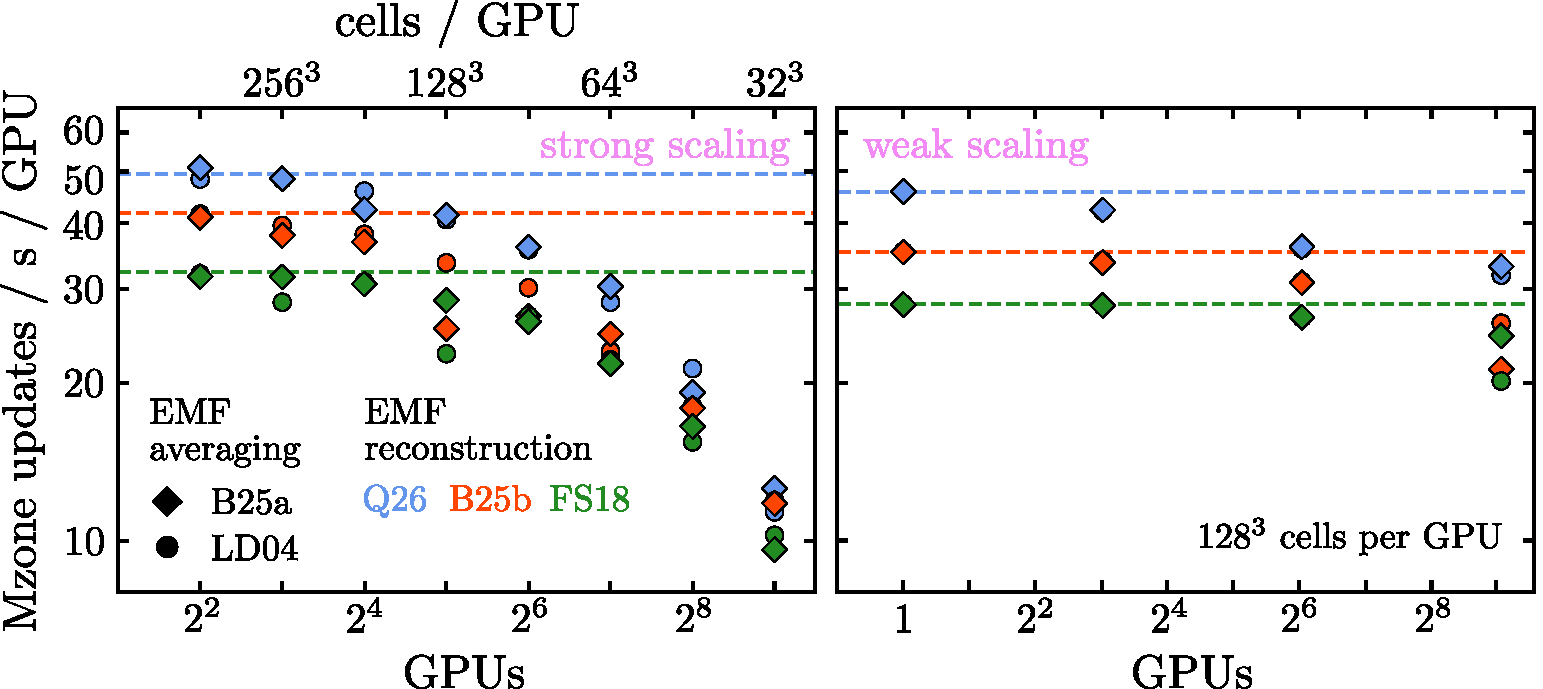
\includegraphics[width=\linewidth]{figures/quokka-mhd/results/scalings.pdf}
%DIFDELCMD <     %%%
%DIFDELCMD < \caption{%
{%DIFAUXCMD
\DIFdelFL{Measured number of zone updates per second per GPU for all schemes as a function of GPU count, for strong scaling at fixed problem size of $512^3$ cells (left) and weak scaling at $128^3$ cells per GPU (right). Blue, green, and red points show the Q26, \mbox{%DIFAUXCMD
\citetalias{Balsara25a}}\hskip0pt%DIFAUXCMD
, and \mbox{%DIFAUXCMD
\citetalias{Felker18a} }\hskip0pt%DIFAUXCMD
EMF reconstruction schemes, while circles and squares show \mbox{%DIFAUXCMD
\citetalias{Londrillo04a} }\hskip0pt%DIFAUXCMD
and \mbox{%DIFAUXCMD
\citetalias{Balsara25b} }\hskip0pt%DIFAUXCMD
EMF averaging, respectively. Dashed horizontal lines indicate perfect scaling for each scheme.}}
    %DIFAUXCMD
%DIFDELCMD < \label{fig:scalings}
%DIFDELCMD < \end{figure}
%DIFDELCMD <

%DIFDELCMD < %%%
\DIFdel{To evaluate the speed of the MHD schemes , we carry out tests of both weak and strong scaling . The test problem we use is a non-grid aligned linear }\DIFdelend \DIFaddbegin \DIFadd{Since the choice of problem for strong and weak scaling is arbitrary, we use the linearly-polarised }\DIFaddend Alfv\'en \DIFdelbegin \DIFdel{wave with $\tilde{\mVector{k}} = \{1,2,3\}$ and $\theta = \pi / 4$, and we solve this problem using the same combinations of reconstruction scheme, averaging scheme, and interpolation method as in }%DIFDELCMD < \autoref{sec:performance:waves}%%%
\DIFdel{. In all cases we evolve the initial configuration }\DIFdelend \DIFaddbegin \DIFadd{wave defined in \sref{sec:scheme-comparison:waves:alfven-linear}, with $\mVector{k} L / 2\pi = \{1, 2, 3\}$ and $\theta = \pi/4$. We evolve each simulation }\DIFaddend for 100 time steps \DIFdelbegin \DIFdel{and measure the speed }\DIFdelend \DIFaddbegin \DIFadd{on the Setonix machine at the Pawsey Supercomputing Centre in Western Australia}\footnote{
    \DIFadd{Each compute node carries four AMD Instinct MI250X GPU cards (two logical GPUs per card), with nodes linked by HPE Slingshot interconnects (allowing direct GPU-to-GPU communication).
}}\DIFadd{, }\DIFaddend excluding startup and I/O \DIFdelbegin \DIFdel{. For the weak scaling test we use a domain of size $(128 \times N_\mathrm{GPU}^{1/3})^3$ for GPU counts of $N_\mathrm{GPU} \in \{1, 8, 64, 512\}$, so that the number of cells per GPU is fixed at $128^3$.
}\DIFdelend \DIFaddbegin \DIFadd{overheads from the measured time.
}

\DIFaddend For strong scaling we \DIFdelbegin \DIFdel{use a fixed problem size of }\DIFdelend \DIFaddbegin \DIFadd{hold the problem size fixed at }\DIFaddend $512^3$ cells \DIFdelbegin \DIFdel{, and test performance at GPU counts of $N_\mathrm{GPU} = 4$ }\DIFdelend \DIFaddbegin \DIFadd{and increase the GPU count from $4$ }\DIFaddend to $512$ in \DIFdelbegin \DIFdel{factor of two steps; we do not carry out strong scaling tests on fewer than four GPUs due to memory size limitations. Thus our strong scaling test uses counts of cells per GPU ranging from $\approx 323^3$ at 4 GPUs to $64^3$ at 512 GPUs.
}%DIFDELCMD <

%DIFDELCMD < %%%
\DIFdel{We report the results of our weak scalingtests in }%DIFDELCMD < \autoref{tab:weak_scaling_zone_update_times_ngpu} %%%
\DIFdel{and our strong scaling tests in }%DIFDELCMD < \autoref{tab:strong_scaling_zone_update_times_ngpu}%%%
\DIFdel{, and plot both results together in }%DIFDELCMD < \autoref{fig:scalings}%%%
\DIFdel{. Our figure of merit for these tests is the cell advance time $t_\mathrm{adv}$, defined as the amount of GPU compute time required to advance one cell for one time step, and its inverse the advance rate }\DIFdelend \DIFaddbegin \DIFadd{doublings. For weak scaling, we use a common local problem size of $128^3$ cells }\DIFaddend per GPU, \DIFdelbegin \DIFdel{$\Gamma = 1/t_\mathrm{adv}$ -- smaller $t_\mathrm{adv}$ and larger $\Gamma_\mathrm{adv}$ are better.
These results enable us to make a few observations.
}\DIFdelend \DIFaddbegin \DIFadd{increasing $N_\mathrm{GPU}$ through $\{1, 8, 64, 512\}$.
}\DIFaddend

\DIFdelbegin \DIFdel{First, the }\DIFdelend \DIFaddbegin \DIFadd{\mbox{%DIFAUXCMD
\Cref{fig:gpu-scaling} }\hskip0pt%DIFAUXCMD
shows that }\DIFaddend Q26 \DIFdelbegin \DIFdel{EMF reconstruction scheme }\DIFdelend is consistently the fastest \DIFdelbegin \DIFdel{across all tests, followed by \mbox{%DIFAUXCMD
\citetalias{Balsara25a} }\hskip0pt%DIFAUXCMD
and then \mbox{%DIFAUXCMD
\citetalias{Felker18a}}\hskip0pt%DIFAUXCMD
. The speed advantage is significant: }\DIFdelend \DIFaddbegin \DIFadd{EMF compute scheme, with a throughput roughly $30\%$ higher than \mbox{%DIFAUXCMD
\citetalias{Balsara25a} }\hskip0pt%DIFAUXCMD
and $60\%$ higher than \mbox{%DIFAUXCMD
\citetalias{Felker18a}}\hskip0pt%DIFAUXCMD
, reaching over $50$ million cell updates per second per GPU at $N_\mathrm{GPU} = 4$. The strong-scaling trends, however, differ between these schemes, following from the different number of ghost zones each requires (\sref{sec:methods:emf:compute}). Although }\DIFaddend Q26 \DIFdelbegin \DIFdel{is $\approx 1.3\times$ faster than the \mbox{%DIFAUXCMD
\citetalias{Balsara25a} }\hskip0pt%DIFAUXCMD
scheme and $\approx 1.6\times$ faster than the \mbox{%DIFAUXCMD
\citetalias{Felker18a} }\hskip0pt%DIFAUXCMD
scheme. These differences persist across node count for both weak and strong scaling, with the exception of strong scaling at the largest node count, where the number of cells per GPU is well below our optimal count (see below). }%DIFDELCMD <

%DIFDELCMD < %%%
\DIFdel{Second, the }\DIFdelend \DIFaddbegin \DIFadd{requires fewer reconstruction steps and temporary variables, evaluating the face velocity in \mbox{%DIFAUXCMD
\cref{eqn:emf:q26-facevel} }\hskip0pt%DIFAUXCMD
requires fluxes over more ghost zones; as a result, the additional work across this larger shell occupies a greater fraction of the update, and its throughput falls off more quickly than for the other schemes, but remains higher than both throughout. By contrast, the choice of }\DIFaddend EMF averaging scheme has almost no effect on \DIFdelbegin \DIFdel{the speed. the reconstruction scheme and reconstruction order are important, but the way that the EMFs are combined at cell corners is not. Again, this is true at all GPU counts and for both weak and strong scaling}\DIFdelend \DIFaddbegin \DIFadd{throughput, since the averaging step changes neither the memory footprint nor the number of GPU kernel launches}\DIFaddend .

\DIFdelbegin \DIFdel{Third, regardless of scheme , the code shows good scaling. Almost all schemes }\DIFdelend \DIFaddbegin \DIFadd{Despite the differences in absolute throughput, most scheme combinations }\DIFaddend achieve better than \DIFdelbegin \DIFdel{70\% weak scaling efficiency }\footnote{\DIFdel{Here we use the usual definition of scaling efficiency, $\epsilon(N_\mathrm{GPU}) = t_\mathrm{adv,min} / t_\mathrm{adv}(N_\mathrm{GPU})$, where $t_\mathrm{adv,min}$ is the advance time on the minimum number of GPUs tested.
}} %DIFAUXCMD
\addtocounter{footnote}{-1}%DIFAUXCMD
\DIFdel{going from 1 to 512 GPUs. The strong scaling efficiency is similarly better than 70\% as long as the number of cells per GPU is }\DIFdelend \DIFaddbegin \DIFadd{$70$\% weak-scaling efficiency from $1$ to $512$ GPUs, and better than $70$\% strong-scaling efficiency when each GPU is assigned at least }\DIFaddend $128^3$ \DIFdelbegin \DIFdel{or more (corresponding to $N_\mathrm{GPU}=64$ for our test setup).
We only see significant scaling efficiency loss at smaller cell counts.
}\DIFdelend \DIFaddbegin \DIFadd{cells.
}\DIFaddend

\subsection{Summary and recommendations}
\DIFdelbegin %DIFDELCMD < \label{sec:performance:summary}
%DIFDELCMD < %%%
\DIFdelend \DIFaddbegin \label{sec:scheme-comparison:recommendation}
\DIFaddend

\DIFdelbegin \DIFdel{For EMF reconstruction, our tests show that our newly-introduced }\DIFdelend \DIFaddbegin \DIFadd{Across all tests, our new }\DIFaddend Q26 scheme \DIFdelbegin \DIFdel{offers the highest speeds and }\DIFdelend \DIFaddbegin \DIFadd{(\sref{sec:methods:emf:compute}) }\DIFaddend produces results in both linear and non-linear problems that are \DIFdelbegin \DIFdel{as good as }\DIFdelend \DIFaddbegin \DIFadd{comparable to those of }\DIFaddend the existing \citetalias{Felker18a} and \citetalias{Balsara25a} schemes\DIFdelbegin \DIFdel{. Its only downside is that it appears to be slightly less stable when combined with higher-order reconstruction methods such as PPM or PPM-EP, and thus may prove unusable for very challenging problems at high order. By contrast the choice of EMF averaging scheme -- \mbox{%DIFAUXCMD
\citetalias{Londrillo04a} }\hskip0pt%DIFAUXCMD
versus \mbox{%DIFAUXCMD
\citetalias{Balsara25b} }\hskip0pt%DIFAUXCMD
-- appears to make little difference to speed, accuracy, or stability. All our comparisons of averaging scheme produce nearly identical results.
}\DIFdelend \DIFaddbegin \DIFadd{, while achieving substantially higher throughput (\sref{sec:scheme-comparison:speed}). Moreover, \mbox{%DIFAUXCMD
\citetalias{Balsara25b} }\hskip0pt%DIFAUXCMD
averaging proved the most stable in reconnection-dominated flows (\sref{sec:scheme-comparison:reconnection}). We therefore adopt Q26 compute with \mbox{%DIFAUXCMD
\citetalias{Balsara25b} }\hskip0pt%DIFAUXCMD
averaging as the default EMF scheme combination in \quokka.
}\DIFaddend

\DIFdelbegin \DIFdel{Based on these findings, our recommendation, which we adopt }\DIFdelend \DIFaddbegin \DIFadd{As for reconstruction order, we broadly find that both PPM and PPM-EP resolve structures in non-linear flows comparably well (\mbox{%DIFAUXCMD
\cref{fig:orszag-tang:reconstruction-schemes}}\hskip0pt%DIFAUXCMD
); however, PPM-EP's extrema-preserving limiter avoids the clipping-induced degradation we found in plain PPM (for some smooth, low-$\mathcal{M}$ waves; \sref{sec:scheme-comparison:waves}). This accuracy comes at a stability cost: PPM-EP remains stable with only two of the six EMF scheme combinations we test in reconnection-dominated flows, compared to all six with plain PPM (\sref{sec:scheme-comparison:reconnection}). We accept this trade-off because one of the two stable combinations is our recommended EMF pairing (Q26 compute with \mbox{%DIFAUXCMD
\citetalias{Balsara25b} }\hskip0pt%DIFAUXCMD
averaging), for which PPM-EP remains stable even in this demanding regime; we therefore recommend PPM-EP }\DIFaddend as the default \DIFdelbegin \DIFdel{in }\textsc{\DIFdel{Quokka}}%DIFAUXCMD
\DIFdel{, is to use Q26 EMF reconstruction together with \mbox{%DIFAUXCMD
\citetalias{Balsara25a} }\hskip0pt%DIFAUXCMD
EMF averaging as the first line method. This is the fastest option by a substantial margin. If this proves to be unstable, one can fall back on \mbox{%DIFAUXCMD
\citetalias{Balsara25b} }\hskip0pt%DIFAUXCMD
EMF reconstruction instead , which is the second-fastest, and is more stable }\DIFdelend \DIFaddbegin \DIFadd{reconstruction scheme specifically alongside this EMF pairing. If a user instead adopts a different EMF combination, plain PPM is the more stable choice, since, unlike PPM-EP, its stability does not depend on which EMF scheme it is paired with}\DIFaddend .


\section{Tests for the recommended scheme}
\DIFdelbegin %DIFDELCMD < \label{sec:tests}
%DIFDELCMD < %%%
\DIFdelend \DIFaddbegin \label{sec:stress-tests}
\DIFaddend

\DIFdelbegin \DIFdel{In this Section we subject or recommended scheme to a series of additional teststhat stress various parts of the algorithm. We use }\DIFdelend \DIFaddbegin \DIFadd{Following the systematic comparison of all three EMF compute schemes (\sref{sec:methods:emf:compute}), both EMF averaging schemes (\sref{sec:methods:emf:averaging}), and three reconstruction schemes (PLM, PPM, PPM-EP) presented in \sref{sec:scheme-comparisons}, we arrive at a recommended combination: Q26 compute with \mbox{%DIFAUXCMD
\citetalias{Balsara25b} }\hskip0pt%DIFAUXCMD
averaging and PPM-EP reconstruction. Because the comparison that supported this conclusion spanned a large number of scheme combinations, it necessarily relied on a core, reduced subset of tests, each chosen to probe differences between schemes rather than to exhaustively validate correctness; this section presents the remainder of that fuller validation suite, run against }\DIFaddend our recommended combination \DIFdelbegin \DIFdel{of Q26 reconstruction plus \mbox{%DIFAUXCMD
\citetalias{Balsara25a} }\hskip0pt%DIFAUXCMD
averaging with PPM-EP interpolation for all the tests presented here unless otherwise noted}\DIFdelend \DIFaddbegin \DIFadd{throughout}\DIFaddend .

\subsection{\DIFdelbegin \DIFdel{Non-grid aligned linear }\DIFdelend \DIFaddbegin \DIFadd{Directional bias in grid-misaligned }\DIFaddend waves}
\DIFdelbegin %DIFDELCMD < \label{sec:tests:misaligned-waves}
%DIFDELCMD < %%%
\DIFdelend \DIFaddbegin \label{sec:stress-tests:misaligned-waves}
\DIFaddend

\DIFdelbegin \DIFdel{We start by demonstrating that our recommended scheme accurately evolves linear waves when they are not aligned with the grid. To this end}\DIFdelend \DIFaddbegin \DIFadd{To test that our solver does not introduce directional bias when waves propagate misaligned, rather than along the grid}\DIFaddend , we simulate \DIFdelbegin \DIFdel{Alfv\'en, fast, and slow MHD waves. The first two of these use the same framework introduced in }%DIFDELCMD < \autoref{sec:performance:waves}%%%
\DIFdel{, where the slow wave was not previously tested, and has an analogous setup, where the perturbed state is of }\DIFdelend the \DIFdelbegin \DIFdel{form
}%DIFDELCMD < \begin{align}
%DIFDELCMD <     &\delta\mVector{S}_\mathrm{c}^{\{\mathrm{sm}\}}
%DIFDELCMD <         = \delta_{a} \cos\sbrac{\omega t - \mVector{k}\cdot\mVector{x}}
%DIFDELCMD <         \nonumber \\
%DIFDELCMD <         &\nquad[1] \begin{Bmatrix}
%DIFDELCMD <             \phi_1 \rho_0 \\
%DIFDELCMD <             c_\mathrm{sm} (
%DIFDELCMD <                     -\phi_1 \mVectorUnit{n}_{k}
%DIFDELCMD <                     + \phi_2 \mVectorUnit{n}_\perp
%DIFDELCMD <                 ) \\
%DIFDELCMD <             \phi_1 p_0 \gamma / (\gamma-1)
%DIFDELCMD <                 + b_0^2\sin\theta
%DIFDELCMD <                 + \delta_{a} \rbrac{
%DIFDELCMD <                         b_0^2 / 2
%DIFDELCMD <                         + \rho_0 c_\mathrm{sm}^2 (\phi_1^2 + \phi_2^2)
%DIFDELCMD <                     } \\
%DIFDELCMD <             b_0 \mVectorUnit{n}_\perp
%DIFDELCMD <         \end{Bmatrix}
%DIFDELCMD <     ,
%DIFDELCMD < \end{align}
%DIFDELCMD < %%%
\DIFdel{where $\mVectorUnit{n}_\perp$ is a unit vector orthogonal to $\mVectorUnit{n}_{k}$ and lying in the plane formed by $\mVectorUnit{n}_{k}$ and $\mVectorUnit{n}_{0}$, }%DIFDELCMD < \begin{align}
%DIFDELCMD <     c_\mathrm{sm}^2
%DIFDELCMD <         = \frac{1}{2}\rbrac{
%DIFDELCMD <             c_\mathrm{s}^2
%DIFDELCMD <             + c_\mathrm{A}^2
%DIFDELCMD <             - \rbrac{
%DIFDELCMD <                     \rbrac{c_\mathrm{s}^2
%DIFDELCMD <                     + c_\mathrm{A}^2}^2
%DIFDELCMD <                     - 4 c_\mathrm{s}^2 c_\mathrm{A}^2 \cos^2\theta
%DIFDELCMD <                 }^{1/2}
%DIFDELCMD <         }
%DIFDELCMD < \end{align}
%DIFDELCMD < %%%
\DIFdel{is the slow magnetosonic wave speed and the geometric factors $\phi_1$ and $\phi_2$ are
}%DIFDELCMD < \begin{align}
%DIFDELCMD <     \phi_1
%DIFDELCMD <         &= \frac{
%DIFDELCMD <             c_\mathrm{sm}^2 - c_\mathrm{A}^2\cos^2\theta
%DIFDELCMD <         }{
%DIFDELCMD <             c_\mathrm{sm}^2 \sin\theta
%DIFDELCMD <         } \\
%DIFDELCMD <     \phi_2
%DIFDELCMD <         &= \rbrac{\frac{c_\mathrm{A}}{c_\mathrm{sm}}}^2 \cos\theta
%DIFDELCMD <     .
%DIFDELCMD < \end{align}
%DIFDELCMD < %%%
\DIFdelend \DIFaddbegin \DIFadd{same slow magnetosonic wave introduced in \sref{sec:scheme-comparison:waves}. We choose this wave because its coupled, compressive perturbations to $\mVector{u}$ and $\mVector{b}$ make it the most stringent test of directional bias among the four waves we test. To probe this, we run it propagating obliquely at $128^3$ and $512^3$, checking whether any directional-bias artefact grows or shrinks with resolution.
}\DIFaddend

\DIFdelbegin \DIFdel{For our tests of non-grid aligned waves, we choose $\tilde{\mVector{k}} = \{1,2,3\}$ and $\theta = \pi / 4$ for all wave types, and simulate for a time }\DIFdelend \DIFaddbegin \DIFadd{We choose $\mVector{k}L/2\pi = \{1, 2, 3\}$ and $\theta \equiv \cos^{-1}\sbrac{\mVectorUnit{n}_\mathrm{bg}\cdot\mVectorUnit{n}_k} = 45^\circ$, so that neither $\mVectorUnit{n}_k$ nor $\mVectorUnit{n}_\mathrm{bg}$ is aligned with any axis of the grid, and simulate until }\DIFaddend $t = 4\pi/\omega$ (\ie two wave periods \DIFdelbegin \DIFdel{) in a domain of }\DIFdelend \DIFaddbegin \DIFadd{$T = 2\pi/\omega$) in domains of $128^3$ and }\DIFaddend $512^3$ cells. \DIFdelbegin \DIFdel{Thus neither the wave vector nor the background magnetic field are aligned with any of the cardinal axes. }\DIFdelend All other parameters are identical to those used in \DIFdelbegin %DIFDELCMD < \autoref{sec:performance:waves}%%%
\DIFdel{, and we also measure the $L_1$ error for our solutions exactly as in that Section. }%DIFDELCMD <

%DIFDELCMD < %%%
\DIFdel{As a representative example, we plot the pencil profiles of the $b_1$ }\DIFdelend \DIFaddbegin \DIFadd{\sref{sec:scheme-comparison:waves}. For this configuration, $\mVectorUnit{n}_\perp = \{-2,1,0\}/\sqrt{5}$, built (as for every wave test) orthogonal to both $\mVectorUnit{n}_k$ and the grid's $x_2$ axis, so it carries no $x_2$ component by construction. With this setup, the wave's magnetic perturbation lies entirely along $\mVectorUnit{n}_\perp$, so $b_0$ carries the dominant share of the wave's magnetic perturbation; since no }\DIFaddend component of the \DIFdelbegin \DIFdel{magnetic field for the slow wave , in }%DIFDELCMD < \autoref{fig:slow-waves}%%%
\DIFdel{.
The slow wave is the most stringent of the three linear wave modes, since its velocity and magnetic perturbations are oblique, compressive, and coupled, so any directional bias in the numerical fluxes would manifest as phase drift or errors in the wave-amplitude. As we show in the pencil profiles, however, after two wave periods, the solution maintains excellent conservation of the amplitude and phase, with an $L_1 = 4.6 \times 10^{-11}$ (at the level of floating-point precision) between the final and initial profiles, which is consistent with the errors we measured for the grid-aligned linear wave tests in }%DIFDELCMD < \autoref{sec:performance:waves}%%%
\DIFdel{.
}\DIFdelend \DIFaddbegin \DIFadd{perturbation contributes to $b_2$, it should remain unperturbed from its background value. In practice, however, this is not guaranteed numerically, so we use growth in $b_2$ as a metric for numerical artefacts: directional bias, seeded when the wave is reconstructed along grid directions it no longer shares. What matters is not $b_2$'s absolute growth, but growth relative to the wave's real signal, carried by $b_0$.
}\DIFaddend

\DIFaddbegin \DIFadd{\mbox{%DIFAUXCMD
\Cref{fig:oblique-slow-wave} }\hskip0pt%DIFAUXCMD
shows the evolution of $b_2$ compared to $b_0$ over the two wave periods, at both resolutions. Since $b_0$ is not constant in space, we do not compare the two fields directly, but rather their total energy (see the figure's y-axis label). Because $b_0$'s total energy is conserved to within $0.3\%$ at both resolutions, changes in the ratio directly follow from growth of $b_2$. At each resolution, the ratio grows over the first wave period as the wave sweeps over cells it has not yet sampled, polluting each with a small numerical deviation from the background state, then saturates once the wave returns to these already-polluted phases on its second period. This saturated ratio shrinks with resolution, as expected, and remains many orders of magnitude below the primary wave throughout, which confirms that the directional bias is not a dynamically significant artefact.
}

\DIFaddend \begin{figure}
    \centering
    \DIFdelbeginFL %DIFDELCMD < 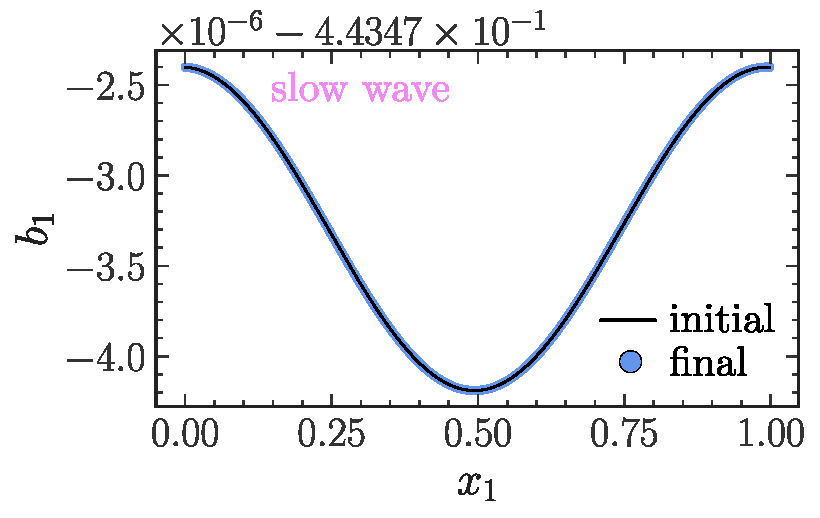
\includegraphics[width=0.65\linewidth]{figures/quokka-mhd/results/slow-Bx-along-x.pdf}
%DIFDELCMD <     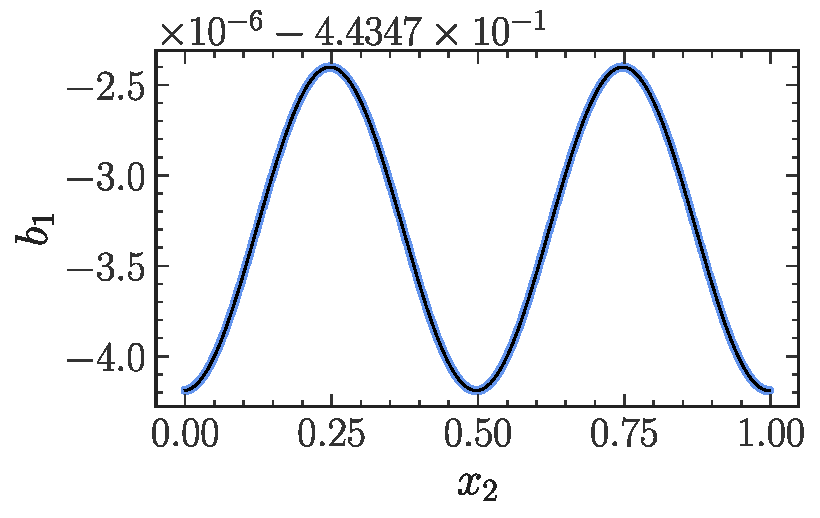
\includegraphics[width=0.65\linewidth]{figures/quokka-mhd/results/slow-Bx-along-y.pdf}
%DIFDELCMD <     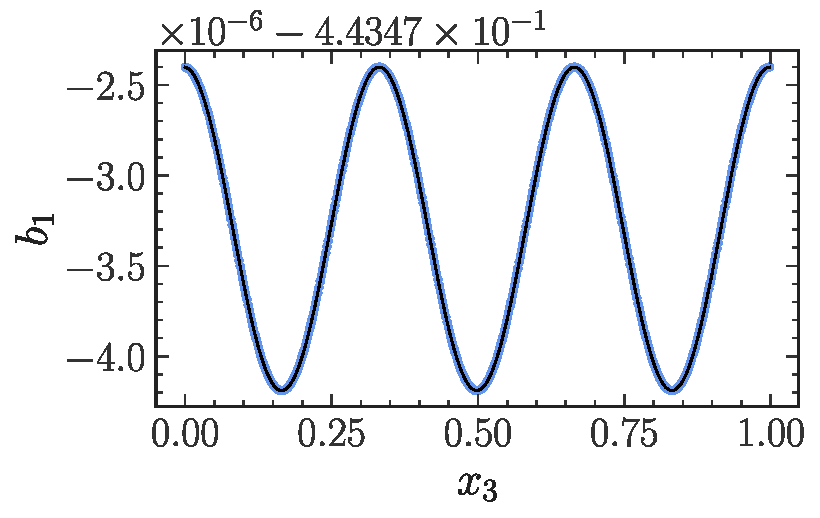
\includegraphics[width=0.65\linewidth]{figures/quokka-mhd/results/slow-Bx-along-z.pdf}
%DIFDELCMD <     %%%
%DIFDELCMD < \caption{%
{%DIFAUXCMD
\DIFdelFL{Representative pencil profiles of the slow wave solution run with $512^3$ cells, comparing the initial profile (black line) against the solution after two wave periods (blue points). We show how the $b_1$ component of the magnetic field varies along the $x_1$ (top), $x_2$ (middle), and $x_3$ (bottom) cardinal axis.}}
    %DIFAUXCMD
%DIFDELCMD < \label{fig:slow-waves}
%DIFDELCMD < %%%
\DIFdelendFL \DIFaddbeginFL 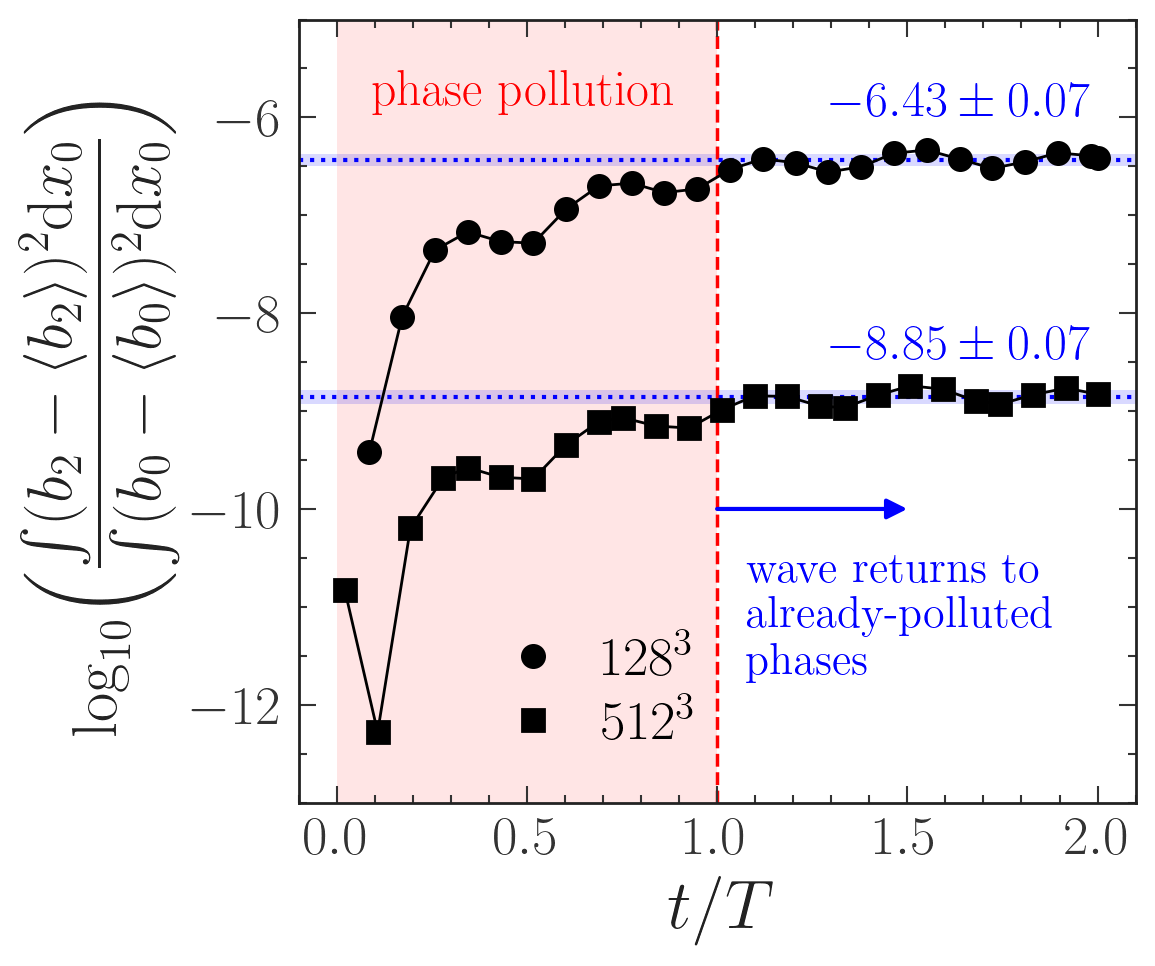
\includegraphics[width=0.65\linewidth]{figures/quokka-mhd/results/slow-wave-polarisation-leakage.png}
    \caption{\DIFaddFL{The oblique slow magnetosonic wave's time-evolving, line-integrated energy ratio of the out-of-plane component, $b_2$, to the component that primarily carries the signal, $b_0$. Both runs use our recommended scheme (Q26 compute, \mbox{%DIFAUXCMD
\citetalias{Balsara25b} }\hskip0pt%DIFAUXCMD
averaging, and PPM-EP reconstruction), at $128^3$ (circles) and $512^3$ (squares). We report the statistically saturated ratio computed over the second wave period, $t/T \geq 1$, where $T$ is the wave period.}}
    \label{fig:oblique-slow-wave}
\DIFaddendFL \end{figure}

%DIF <  \subsection{Current sheet}
\DIFaddbegin \subsection{\DIFadd{Stability of odd-even decoupling}}
\label{sec:stress-tests:quirk}
\DIFaddend

\DIFdelbegin \subsection{\DIFdel{Balsara vortex}}
%DIFAUXCMD
\addtocounter{subsection}{-1}%DIFAUXCMD
%DIFDELCMD < \label{sec:tests:balsara-vortex}
%DIFDELCMD < %%%
\DIFdelend \DIFaddbegin \begin{figure}
    \centering
    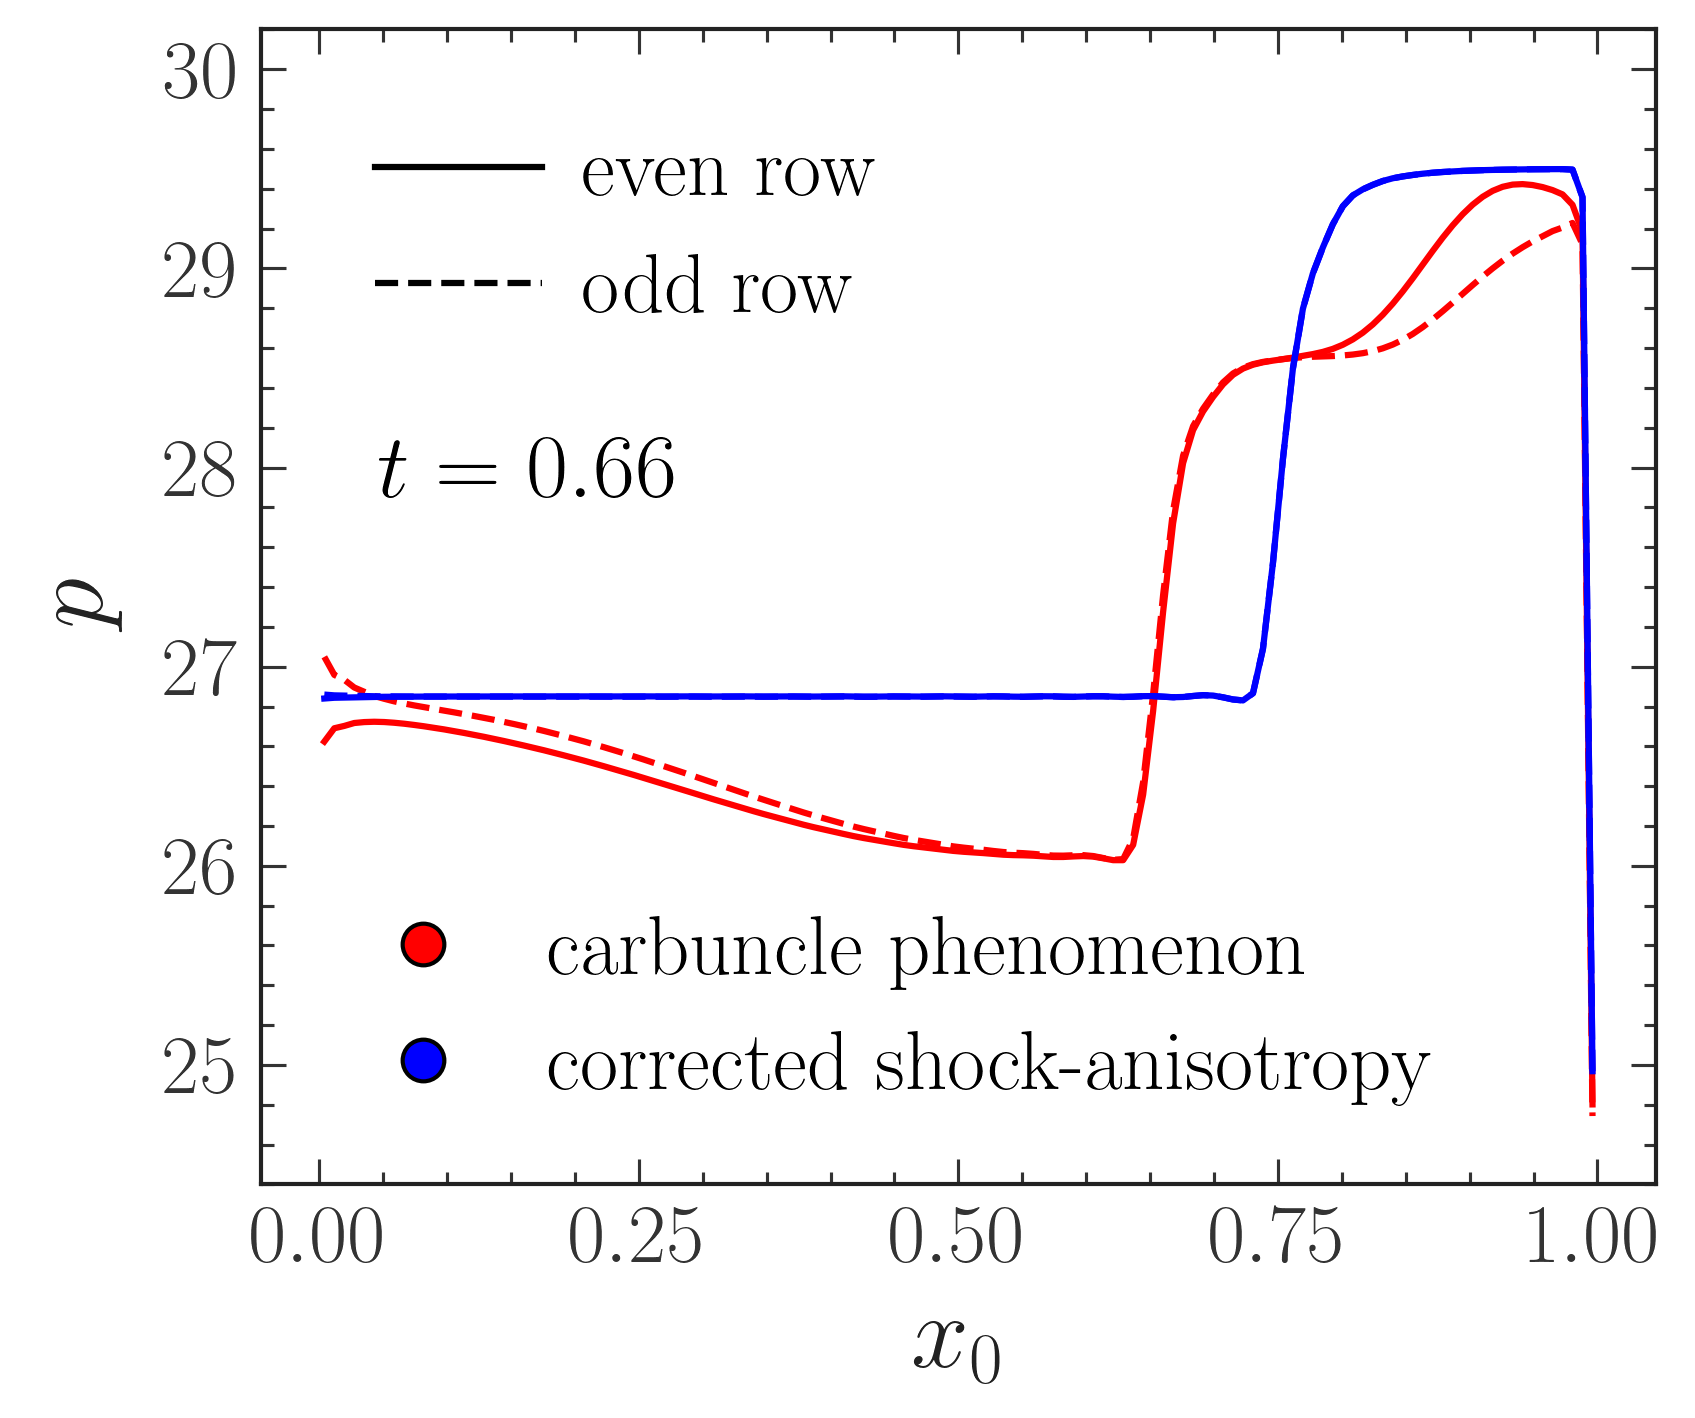
\includegraphics[width=0.65\linewidth]{figures/quokka-mhd/results/quirk-odd-even-split.png}
    \caption{\DIFaddFL{The \mbox{%DIFAUXCMD
\citet{Quirk94a} }\hskip0pt%DIFAUXCMD
odd-even decoupling test (\sref{sec:stress-tests:quirk}), run with our recommended scheme (Q26 compute, \mbox{%DIFAUXCMD
\citetalias{Balsara25b} }\hskip0pt%DIFAUXCMD
averaging, and PPM-EP reconstruction) at $128^2$ resolution, at $t \approx 0.66$. We show profiles of pressure along the $x_0$-axis for one of the perturbed rows (solid line; even $x_1$-index) and one unperturbed row (dashed line; odd $x_1$-index), with the \mbox{%DIFAUXCMD
\citet{Minoshima21a} }\hskip0pt%DIFAUXCMD
shock-anisotropy correction disabled (red) and enabled (blue).}}
    \label{fig:quirk-carbuncle}
\end{figure}
\DIFaddend

\DIFdelbegin \DIFdel{Our next test is the \mbox{%DIFAUXCMD
\citet{Balsara04a} }\hskip0pt%DIFAUXCMD
vortex}\DIFdelend \DIFaddbegin \DIFadd{Next we test a complementary regime to \sref{sec:stress-tests:misaligned-waves}: rather than a wave misaligned with the grid, we now consider a shock deliberately aligned with it. This is because, in low-dissipation Riemann solvers applied dimension-by-dimension (like our HLLD solver), pressure perturbations transverse to the direction being solved are dissipated less than those aligned with it. When this is left unaddressed, even small perturbations at shock fronts can grow into corrugated, non-planar instabilities \mbox{%DIFAUXCMD
\citep{Quirk94a, Minoshima21a}}\hskip0pt%DIFAUXCMD
. Fortunately, a solution exists: a shock-anisotropy correction \mbox{%DIFAUXCMD
\citep{Minoshima21a} }\hskip0pt%DIFAUXCMD
(\sref{sec:methods:flux}), which we have extended our HLLD solver to include. Here we verify, using the \mbox{%DIFAUXCMD
\citet{Quirk94a} }\hskip0pt%DIFAUXCMD
test problem, that our Riemann solver with this correction avoids forming this }\emph{\DIFadd{carbuncle}} \DIFadd{instability.
}

\DIFadd{The test we use is a strong, planar shock initialised at $x_0 = 0.4$ within a domain $x_0, x_1 \in [0,1]$, with $\gamma = 5/3$, and run with $128^2$ cells. We use outflowing (Dirichlet) boundary conditions in $x_0$ and periodic boundary conditions in $x_1$ (and $x_2$; see \mbox{%DIFAUXCMD
\cref{note:quokka:3d}}\hskip0pt%DIFAUXCMD
). We initialise the post-shock region, $x_0 \leq 0.4$, as:
}\begin{align}
    \mVector{S}_\mathrm{c}^{[L; \mathrm{bg}]}
        = \begin{Bmatrix}
                \rho \\
                u_0 \\
                p
            \end{Bmatrix}
        = \begin{Bmatrix}
                3.692 \\
                -0.625 \\
                26.85
            \end{Bmatrix}
    ,
\end{align}
\DIFadd{and the pre-shock region, $x_0 > 0.4$, as:
}\begin{align}
    \mVector{S}_\mathrm{c}^{[R]}
        = \begin{Bmatrix}
                \rho \\
                u_0 \\
                p
            \end{Bmatrix}
        = \begin{Bmatrix}
                1 \\
                -5 \\
                0.6
            \end{Bmatrix}
    ,
\end{align}
\DIFadd{with $\mVector{b} = \mVector{0}$ and $u_1 = u_2 = 0$; this corresponds with a pre-shock sonic Mach number $\mathcal{M} = 5$. Following \mbox{%DIFAUXCMD
\citet{Quirk94a}}\hskip0pt%DIFAUXCMD
, we perturb the post-shock state in every even $x_1$-index cell, at $x_0 = 0.4$ as:
}\begin{align}
    \mVector{S}_\mathrm{c}^{[L; \delta]}
        = \begin{Bmatrix}
                \delta\rho \\
                \delta u_0 \\
                \delta p
            \end{Bmatrix}
        = \begin{Bmatrix}
                -0.135 \\
                0.219 \\
                -1.31
            \end{Bmatrix}
    ,
\end{align}
\DIFadd{where odd $x_1$-index cells remain unperturbed. The complete post-shock state is then $\mVector{S}_\mathrm{c}^{[L]} = \mVector{S}_\mathrm{c}^{[L; \mathrm{bg}]} + \mVector{S}_\mathrm{c}^{[L; \delta]}$}\DIFaddend .
\DIFaddbegin

\DIFadd{We run this test using $\mathrm{CFL} = 0.2$, and compare our recommended scheme with a version of this same scheme where the correction of \mbox{%DIFAUXCMD
\citet{Minoshima21a} }\hskip0pt%DIFAUXCMD
is not included. In \mbox{%DIFAUXCMD
\cref{fig:quirk-carbuncle} }\hskip0pt%DIFAUXCMD
we plot pressure profiles at $t \approx 0.66$, along $x_0$ for both an even $x_1$-index (where the perturbation was applied; solid line) and an odd $x_1$-index (unperturbed; dashed line); we show the run without the correction in red, and the run with the correction in blue. Without the correction, the even and odd rows drift apart, and the shock itself deforms, becoming broader and less sharp. The run with the correction shows neither of these two features: the \mbox{%DIFAUXCMD
\citet{Minoshima21a} }\hskip0pt%DIFAUXCMD
shock-anisotropy correction is both necessary and effective at suppressing the carbuncle instability.
}

\subsection{\DIFadd{Energy conservation at low Mach number}}
\label{sec:stress-tests:balsara-vortex}

\DIFadd{At low $\mathcal{M}$, approximate Riemann solvers get the pressure scaling wrong \mbox{%DIFAUXCMD
\citep{GuillardMurrone04a, watt2025mitigating}}\hskip0pt%DIFAUXCMD
: the dissipation needed for upwind stability, set by the fast magnetosonic wave speed, scales as $\bigO{\mathcal{M}}$, while the true pressure signal scales as $\bigO{\mathcal{M}^2}$. At typical astrophysical $\mathcal{M}$, this dissipation is sufficient, but as $\mathcal{M} \to 0$, it comes to dominate and dynamics can misbehave. As with the carbuncle fix in \sref{sec:stress-tests:quirk}, \mbox{%DIFAUXCMD
\citet{Minoshima21a} }\hskip0pt%DIFAUXCMD
provide a fix here too: a low-$\mathcal{M}$ pressure rescaling. We have implemented this correction, and here validate it against the \mbox{%DIFAUXCMD
\citet{Balsara04a} }\hskip0pt%DIFAUXCMD
vortex; we deliberately do not test at higher resolution, since resolution alone is also a way to resolve away this kind of issue.
}

\DIFaddend We initialise a \DIFdelbegin \DIFdel{steady-state flow field centred }\DIFdelend \DIFaddbegin \DIFadd{stable equilibrium vortex }\DIFaddend in a periodic domain \DIFdelbegin \DIFdel{$\mVector{x} \in [(-5, -5, -\Delta x/2), (5, 5, \Delta x/2)]$, and advect it diagonally by adding a uniform drift velocity,
}%DIFDELCMD < \begin{align}
%DIFDELCMD <     \mVector{u}(\mVector{x})
%DIFDELCMD <         &= \mVector{u}_\mathrm{drift} + \mVector{u}_\mathrm{vortex} \\
%DIFDELCMD <     \mVector{u}_\mathrm{drift}(\mVector{x})
%DIFDELCMD <         &= \frac{\tilde{u}}{\sqrt{2}} \rbrac{\mVectorUnit{x}_1 + \mVectorUnit{x}_2} \\
%DIFDELCMD <     \mVector{u}_\mathrm{vortex}(\mVector{x})
%DIFDELCMD <         &= \tilde{u} \rbrac{x_1 \mVectorUnit{x}_2 - x_2 \mVectorUnit{x}_1} \exp\sbrac{\frac{1 - r^2}{2}} \\
%DIFDELCMD <     \mVector{b}(\mVector{x})
%DIFDELCMD <         &= \tilde{b} \rbrac{x_1 \mVectorUnit{x}_2 - x_2 \mVectorUnit{x}_1} \exp\sbrac{\frac{1 - r^2}{2}} \\
%DIFDELCMD <     p(\mVector{x})
%DIFDELCMD <         &= p_0 + \rbrac{
%DIFDELCMD <                 \frac{\tilde{b}^2}{2} (1 - r^2) - \frac{\rho_0 \tilde{u}^2}{2}
%DIFDELCMD <             } \exp\sbrac{1 - r^2} \\
%DIFDELCMD <     \rho(\mVector{x})
%DIFDELCMD <         &= \rho_0
%DIFDELCMD <     ,
%DIFDELCMD < \end{align}%%%
\DIFdelend \DIFaddbegin \DIFadd{spanning $x_0, x_1 \in [-5, 5]$, with $\gamma = 5/3$, and, to further stress the solver, advect the vortex diagonally along the grid,
}\begin{align}
    \rho(\mVector{x})
        &= \rho_\mathrm{bg} \\
    \mVector{u}(\mVector{x})
        &= \mVector{u}_\mathrm{drift}
            + \mVector{u}_\mathrm{vortex} \\
    p(\mVector{x})
        &= p_\mathrm{bg} + \frac{1}{2} \rbrac{
                \delta b^2 (1 - r^2)
                - \rho_\mathrm{bg} (\delta u)^2
            } \exp\sbrac{1 - r^2} \\
    \mVector{b}(\mVector{x})
        &= \delta b \rbrac{
                x_0 \mVectorUnit{x}_1
                - x_1 \mVectorUnit{x}_0
            } \exp\sbrac{\frac{1 - r^2}{2}}
    ,
\end{align}\DIFaddend
where\DIFdelbegin \DIFdel{$r^2 = x_1^2 + x_2^2$}\DIFdelend \DIFaddbegin \DIFadd{,
}\begin{align}
    \mVector{u}_\mathrm{drift}(\mVector{x})
        &= \frac{\delta u}{\sqrt{2}} \rbrac{
                \mVectorUnit{x}_0
                + \mVectorUnit{x}_1
            } \\
    \mVector{u}_\mathrm{vortex}(\mVector{x})
        &= \delta u \rbrac{
                x_0 \mVectorUnit{x}_1
                - x_1 \mVectorUnit{x}_0
            } \exp\sbrac{\frac{1 - r^2}{2}}
        ,
\end{align}
\DIFadd{with $r^2 = x_0^2 + x_1^2$}\DIFaddend . In our implementation, we adopt a background state \DIFdelbegin \DIFdel{$\rho_0 = 1$, $p_0 = 1$, and $\gamma = 5/3$, so $c_\mathrm{s} = \sqrt{\gamma p_0 / \rho_0} = \sqrt{5/3}$}\DIFdelend \DIFaddbegin \DIFadd{$\rho_\mathrm{bg} = 1$ and $p_\mathrm{bg} = 1$, so $c_\mathrm{s} = \sqrt{\gamma p_\mathrm{bg} / \rho_\mathrm{bg}} = \sqrt{5/3}$}\DIFaddend . We parametrise the vortex velocity amplitude as \DIFdelbegin \DIFdel{$\tilde{u} = \mathcal{M} c_\mathrm{s}$, and choose $\mathcal{M} = 0.01$.
We set $\tilde{b} = \tilde{u}$ to ensure MHD force balance (}%DIFDELCMD < \ie %%%
\DIFdel{magnetic tension exactly balances the centrifugal force associated with the vortex).
}\DIFdelend \DIFaddbegin \DIFadd{$\delta u = \mathcal{M} c_\mathrm{s}$, choosing $\mathcal{M} = \delta b = 0.01$.
}\DIFaddend

Under these conditions, \ie \DIFdelbegin \DIFdel{$p_0 - \rho_0 \tilde{u}^2 / 2 > 0$}\DIFdelend \DIFaddbegin \DIFadd{$p_\mathrm{bg} - \rho_\mathrm{bg} (\delta u)^2 / 2 > 0$}\DIFaddend , or equivalently $\mathcal{M} < \sqrt{2 / \gamma} = \sqrt{6/5}$, the vortex is an exact equilibrium solution \DIFdelbegin \DIFdel{of }\DIFdelend \DIFaddbegin \DIFadd{to }\DIFaddend the ideal MHD equations. Thus the \DIFaddbegin \DIFadd{flow's }\DIFaddend total kinetic, magnetic, and internal energy \DIFdelbegin \DIFdel{of the flow }\DIFdelend should remain constant\DIFdelbegin \DIFdel{over time. Checking the }\DIFdelend \DIFaddbegin \DIFadd{. The }\DIFaddend extent to which \DIFdelbegin \DIFdel{each of these energies is }\DIFdelend \DIFaddbegin \DIFadd{these quantities are }\DIFaddend conserved is therefore a very strong diagnostic of \DIFdelbegin \DIFdel{the level of }\DIFdelend numerically induced dissipation as the vortex advects relative to the grid.
\DIFdelbegin \DIFdel{It is particularly effective for testing dissipation at low $\mathcal{M}$, and thus for checking the effectiveness of the low-Mach pressure rescaling fix \mbox{%DIFAUXCMD
\citep{Minoshima21a} }\hskip0pt%DIFAUXCMD
described in }%DIFDELCMD < \autoref{sec:methods:flux}%%%
\DIFdel{.
}\DIFdelend

We run the test at two resolutions, \DIFdelbegin \DIFdel{$64 \times 64 \times 8$ and $128 \times 128 \times 8$, and run to time $t = 30\sqrt{2}/\tilde{u}$, }\DIFdelend \DIFaddbegin \DIFadd{$64^2$ and $128^2$, to $t = 30\sqrt{2}/\delta u$, which is }\DIFaddend long enough for the vortex to advect diagonally across the periodic domain three times. \DIFdelbegin \DIFdel{We find that our recommended scheme -- Q26 reconstruction, \mbox{%DIFAUXCMD
\citetalias{Balsara25a} }\hskip0pt%DIFAUXCMD
averaging, and PPM-EP interpolation -- performs exceptionally well. }\DIFdelend At \DIFdelbegin \DIFdel{$64 \times 64 \times 8$ resolution, we find that the magnetic energy at the end of the simulation is $92.5\%$ of its initial value; at $128 \times 128 \times 8$ resolution this increases to $99.5\%$. }%DIFDELCMD < \autoref{fig:balsara-vortex} %%%
\DIFdel{shows that the vortex maintains its shape extremely well, as well, even for the lower of our two tested resolutions.
The level of energy conservation we achieve is comparable to that achieved by \mbox{%DIFAUXCMD
\citet{watt2025mitigating} }\hskip0pt%DIFAUXCMD
using a customised MHD solver optimised for conservation in the }\DIFdelend \DIFaddbegin \DIFadd{$64^2$, we find that the magnetic energy retains $92.0\%$ of its energy per orbit, and at $128^2$ it retains $99.6\%$ per orbit; this is comparable to what \mbox{%DIFAUXCMD
\citet{watt2025mitigating} }\hskip0pt%DIFAUXCMD
achieved using a custom MHD solver optimised specifically for this }\DIFaddend low-$\mathcal{M}$ \DIFdelbegin \DIFdel{regime. }\DIFdelend \DIFaddbegin \DIFadd{regime. This is summarised in \mbox{%DIFAUXCMD
\cref{fig:balsara-vortex}}\hskip0pt%DIFAUXCMD
, where we show the vortex for both resolutions ($64^2$ on the left, and $128^2$ on the right), comparing the initial profile (top panels) to the final (bottom panels). The profiles retain both their amplitude and shape extremely well; we needed to take the $\log_{10}$ of the amplitude to reveal the warping effect at $64^2$, which is completely gone at $128^2$, confirming that the \mbox{%DIFAUXCMD
\citet{Minoshima21a} }\hskip0pt%DIFAUXCMD
low-Mach pressure rescaling fix works as intended.
}\DIFaddend

\begin{figure}
    \centering
    \DIFdelbeginFL %DIFDELCMD < 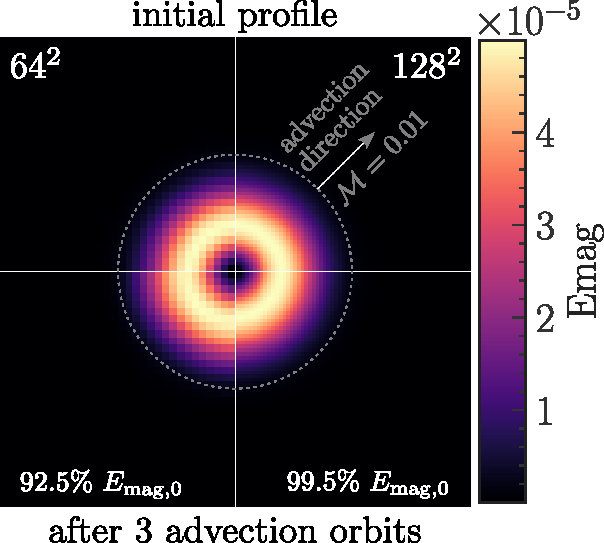
\includegraphics[width=0.65\linewidth]{figures/quokka-mhd/results/balsara-vortex.pdf}
%DIFDELCMD <     \caption{%%%
\DIFdelFL{Slices of magnetic energy density in the Balsara vortex problem run }\DIFdelendFL \DIFaddbeginFL 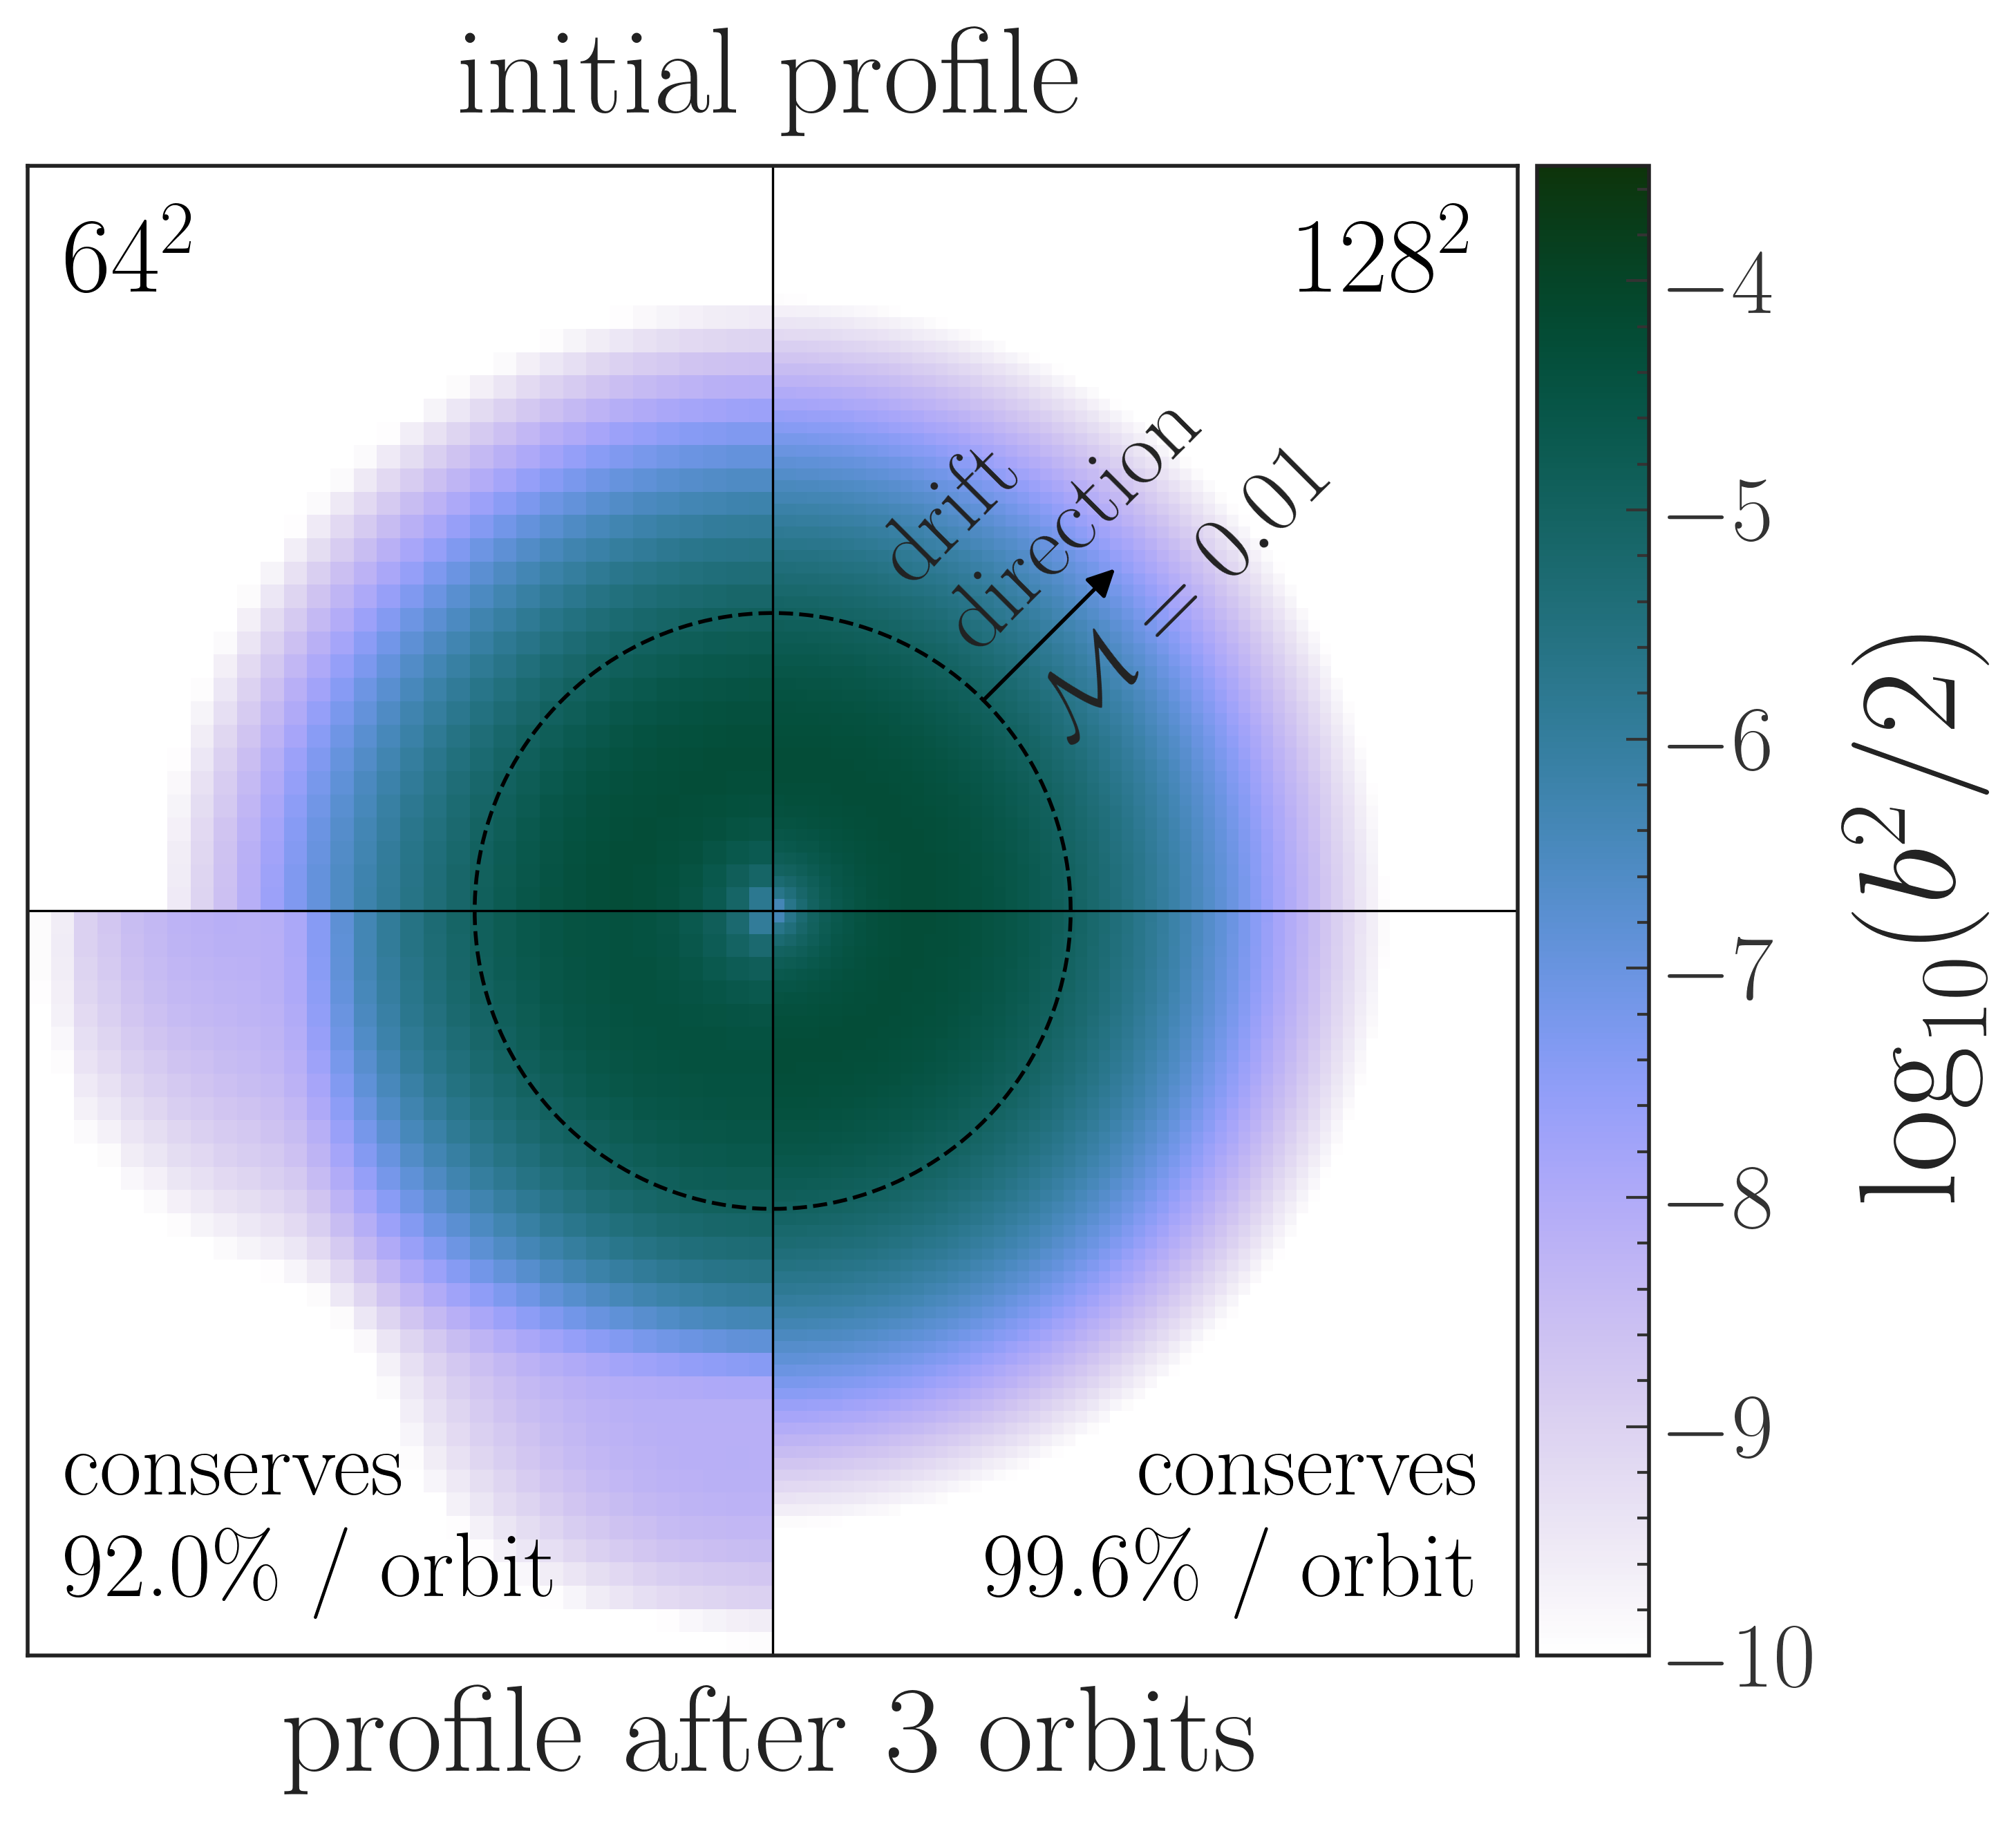
\includegraphics[width=0.65\linewidth]{figures/quokka-mhd/results/balsara-vortex-resolution-comparison.png}
    \caption{\DIFaddFL{Slices of magnetic energy density in the \mbox{%DIFAUXCMD
\citet{Balsara04a} }\hskip0pt%DIFAUXCMD
vortex (\sref{sec:stress-tests:balsara-vortex}), run with $\mathcal{M} = 0.01$ using our recommended scheme (Q26 compute, \mbox{%DIFAUXCMD
\citetalias{Balsara25b} }\hskip0pt%DIFAUXCMD
averaging, and PPM-EP reconstruction). Each quadrant of the domain reveals a different solution: $64^2$ on the left and $128^2$ on the right, the initial condition on top and the final state after $3$ completed advection periods on the bottom. A reference circle (radius $=2$) shows the energy containing portion of the vortex; we indicate the measured fraction of magnetic energy retained per orbit.}}
    \label{fig:balsara-vortex}
\end{figure}

\subsection{\DIFadd{3D shock robustness}}
\label{sec:stress-tests:blast-wave}

\DIFadd{Our next test is a 3D magnetised blast wave \mbox{%DIFAUXCMD
\citep{BalsaraSpicer99a}}\hskip0pt%DIFAUXCMD
, }\DIFaddend with \DIFdelbegin \DIFdel{$\mathcal{M} = 0.01$ using Q26 reconstruction coupled with \mbox{%DIFAUXCMD
\citetalias{Balsara25a} }\hskip0pt%DIFAUXCMD
averaging }\DIFdelend \DIFaddbegin \DIFadd{$\gamma = 5/3$ in a periodic domain $x_0,x_1,x_2 \in [-0.5,0.5]$. We initialise an overpressured spherical region, threaded by a strong background magnetic field oriented obliquely to the grid, to stress shock propagation across a range of angles to both the mesh and the field,
}\begin{align}
    \rho(\mVector{x})
        &= 1 \\
    \mVector{u}(\mVector{x})
        &= 0 \\
    p(\mVector{x})
        &= \begin{cases}
                100
                    & , \qquad r < R \\
                1
                    & , \qquad r \geq R
            \end{cases} \\
    \mVector{b}(\mVector{x})
        &= \frac{10}{\sqrt{2}} \rbrac{\mVectorUnit{x}_0 + \mVectorUnit{x}_1}
    ,
\end{align}
\DIFadd{where $r = \rbrac{x_0^2 + x_1^2 + x_2^2}^{1/2}$ }\DIFaddend and \DIFdelbegin \DIFdel{PPM-EP reconstruction}\DIFdelend \DIFaddbegin \DIFadd{$R = 0.125$}\DIFaddend .
\DIFdelbegin \DIFdel{We show the simulation run at $64 \times 64 \times 8$ on the left }\DIFdelend \DIFaddbegin

\begin{figure}
    \centering
    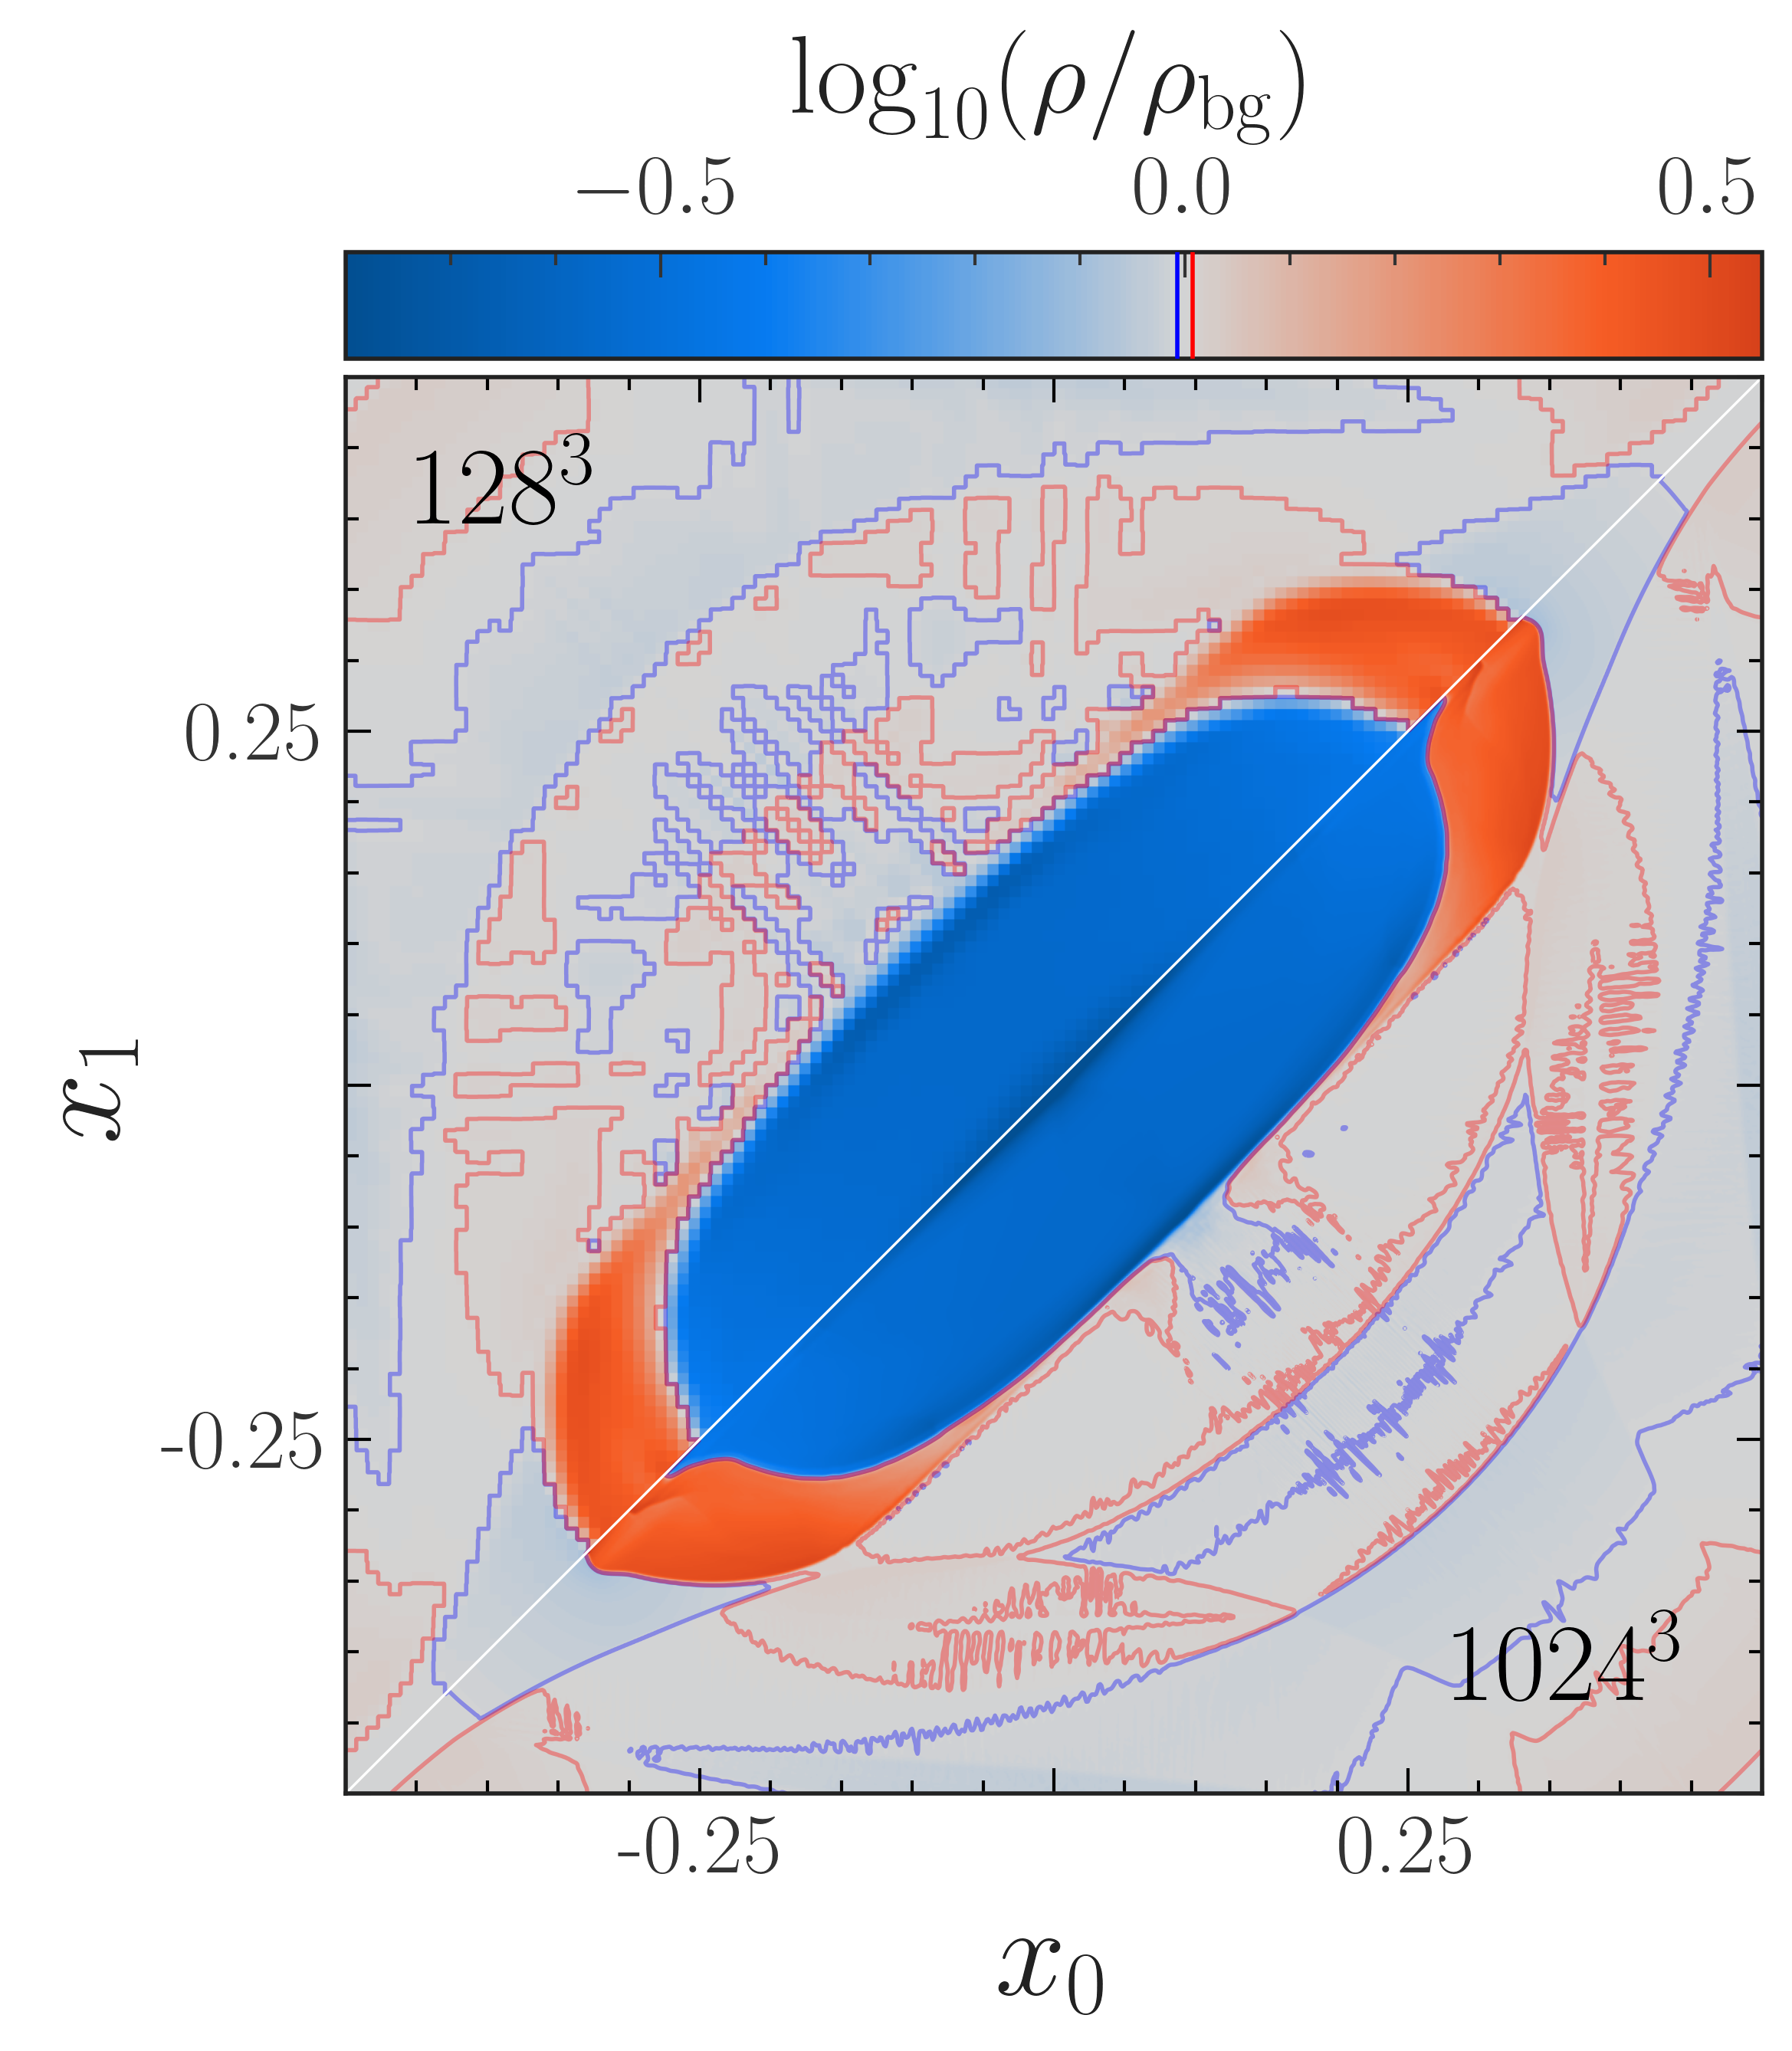
\includegraphics[width=0.65\linewidth]{figures/quokka-mhd/results/blast-wave-resolution-comparison.png}
    \caption{\DIFaddFL{Density slices for the \mbox{%DIFAUXCMD
\citet{BalsaraSpicer99a} }\hskip0pt%DIFAUXCMD
blast wave (\sref{sec:stress-tests:blast-wave}) through the mid-plane at $t = 0.05$, normalised by the ambient background value; run with our recommended scheme (Q26 compute, \mbox{%DIFAUXCMD
\citetalias{Balsara25b} }\hskip0pt%DIFAUXCMD
averaging, and PPM-EP reconstruction). We compare $128^3$ (upper-left half) with $1024^3$ (in the lower-right), and show contours at $\log_{10}(\rho/\rho_\mathrm{bg}) = \pm 0.0075$.}}
    \label{fig:blast-wave}
\end{figure}

\DIFadd{We run this test to $t = 0.05$ both at $128^3$ }\DIFaddend and \DIFaddbegin \DIFadd{$1024^3$, and find that both runs remain stable at full high-order accuracy, even in the $1024^3$ run where substantially sharper gradients are resolved than in $128^3$. \mbox{%DIFAUXCMD
\Cref{fig:blast-wave} }\hskip0pt%DIFAUXCMD
shows both resolutions side by side, with contours overlaid to trace faint ($\lesssim 2\%$) density perturbations left by fast magnetosonic waves, the only visible imprint of the shock's passage at either resolution.
}

\subsection{\DIFadd{Resolved tearing-mediated reconnection}}
\label{sec:stress-tests:current-sheet}

\DIFadd{We validate our recommended scheme's ability to resolve tearing-mediated reconnection in two settings: the current sheet problem introduced in \sref{sec:scheme-comparison:reconnection}, and a higher-resolution repeat of the Orszag-Tang vortex from \sref{sec:scheme-comparison:orszag-tang}.
}

\begin{figure}
    \centering
    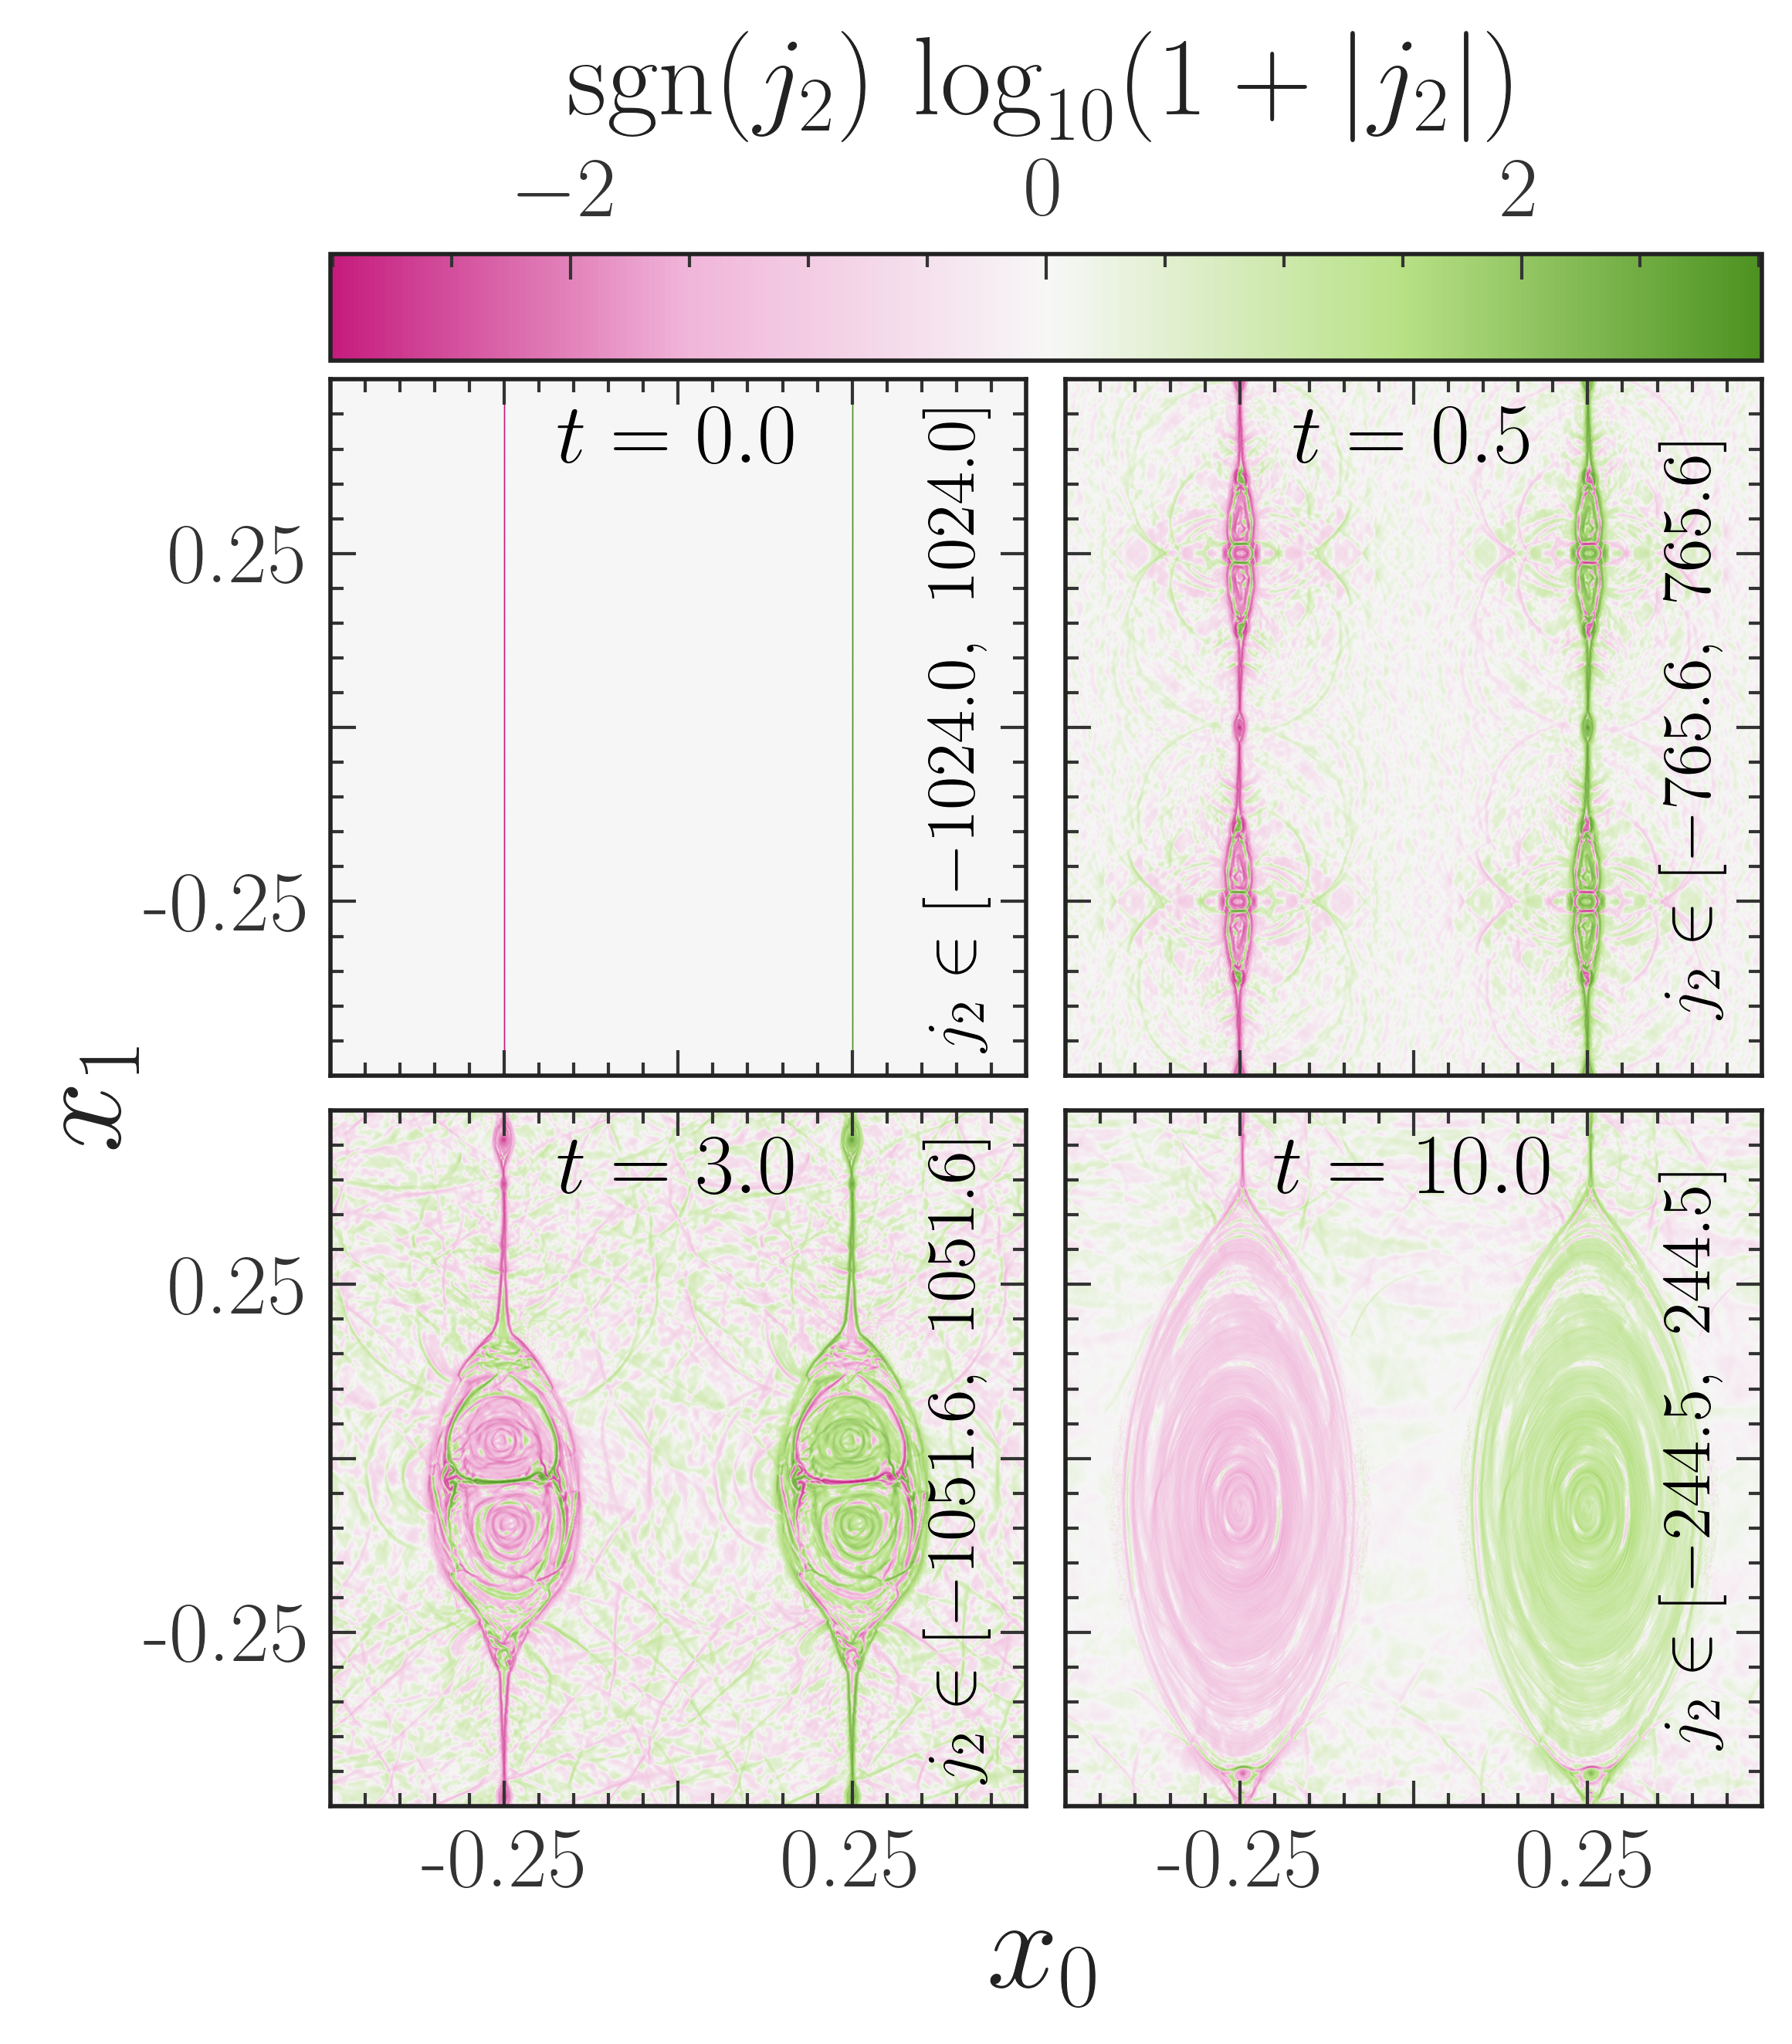
\includegraphics[width=0.65\linewidth]{figures/quokka-mhd/results/current-sheet-current-density-evolution.png}
    \caption{\DIFaddFL{Evolution of the out-of-plane current density component $j_2 = \rbrac{\nabla \times \mVector{b}}_2$ for the \mbox{%DIFAUXCMD
\citet{HawleyStone95a} }\hskip0pt%DIFAUXCMD
current sheet problem (\sref{sec:stress-tests:current-sheet}), run at $1024^2$ with our recommended scheme (Q26 compute, \mbox{%DIFAUXCMD
\citetalias{Balsara25b} }\hskip0pt%DIFAUXCMD
averaging, and PPM-EP reconstruction). We show slices at $t = 0$, $0.5$, $3$, and $10$. Colours show the signed-logarithmic value of $j_2$; the annotation along the right edge of each panel shows the minimum and maximum $j_2$ in each snapshot.}}
    \label{fig:current-sheet}
\end{figure}

\begin{sidewaysfigure}
    \centering
    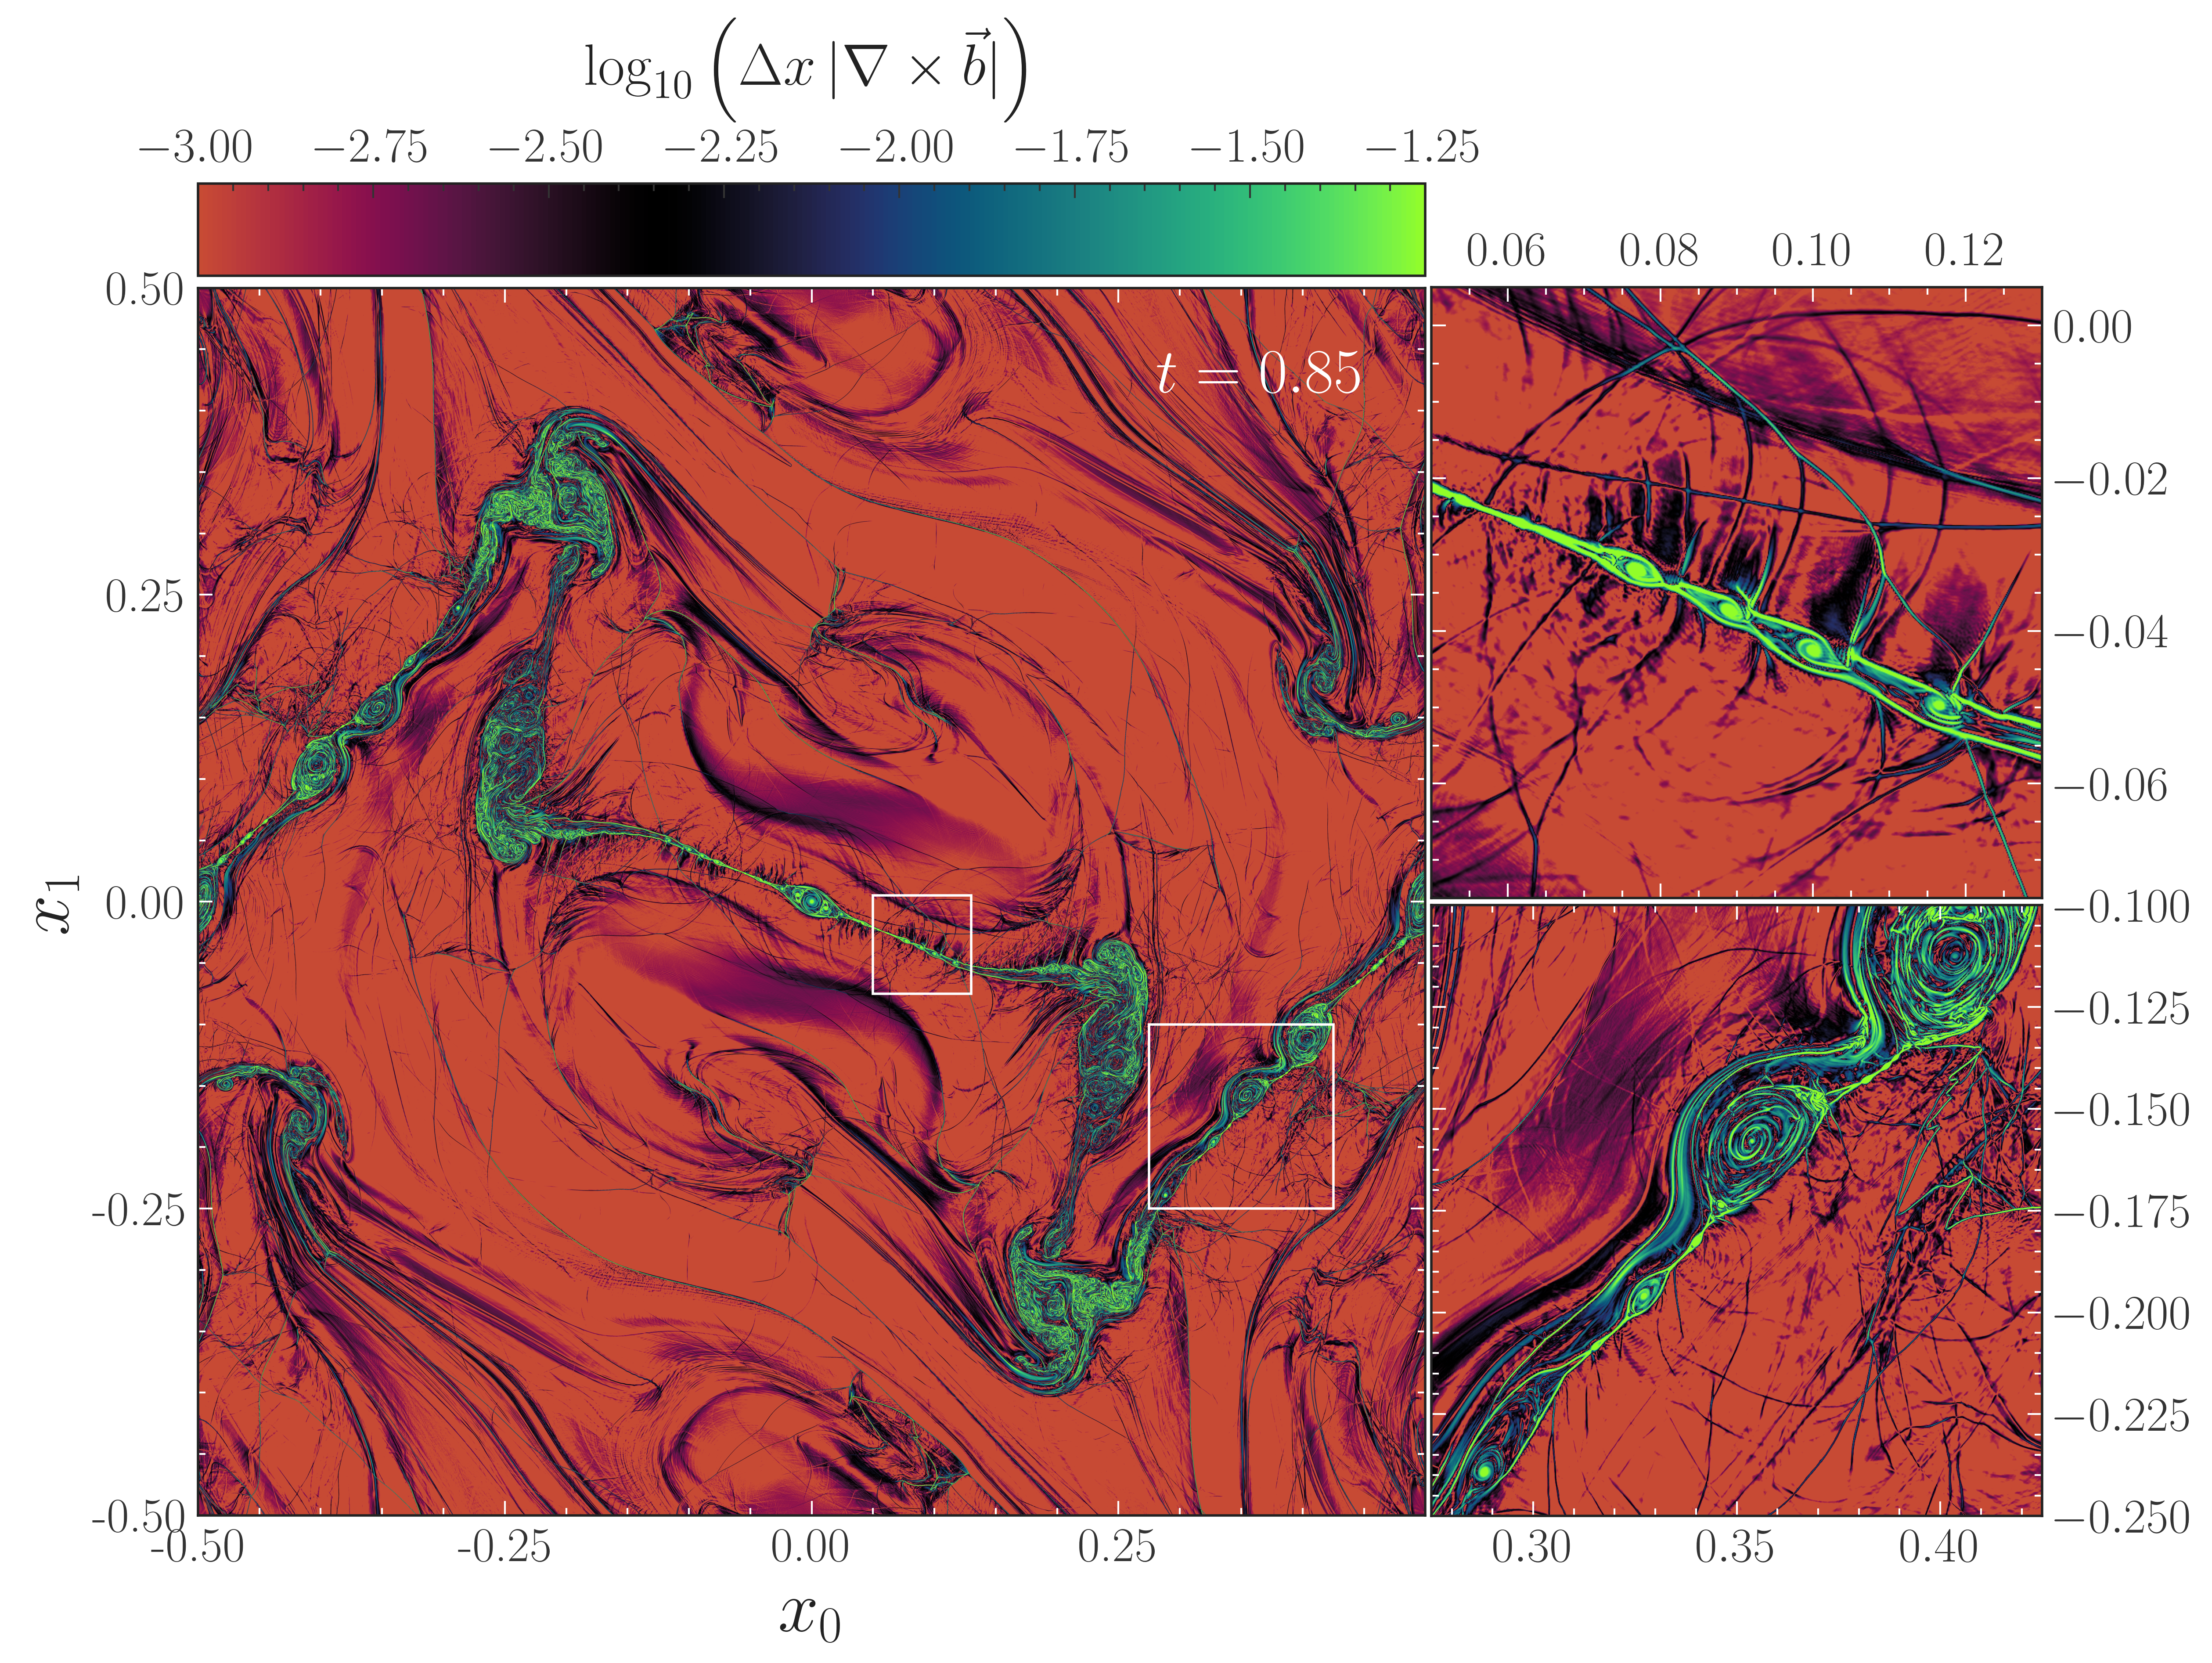
\includegraphics[width=0.8\textheight]{figures/quokka-mhd/results/orszag-tang-structure-zoomins.png}
    \caption{\DIFadd{Current density magnitude, $\log_{10}\rbrac{\Delta x\, |\nabla\times\mVector{b}|}$, for the Orszag-Tang vortex (\sref{sec:scheme-comparison:orszag-tang:setup}) at $8192^2$ and $t=0.85$, run with our recommended scheme (Q26 compute, \mbox{%DIFAUXCMD
\citetalias{Balsara25b} }\hskip0pt%DIFAUXCMD
averaging, and PPM-EP reconstruction). White boxes on the full-domain panel (left) mark the two regions showing zoomed insets (right).}}
    \label{fig:orszag-tang:zoomins}
\end{sidewaysfigure}

\DIFadd{Having shown in \sref{sec:scheme-comparison:reconnection} that our recommended scheme is one of only two EMF scheme combinations that remain stable with PPM-EP reconstruction for the \mbox{%DIFAUXCMD
\citet{HawleyStone95a} }\hskip0pt%DIFAUXCMD
and \mbox{%DIFAUXCMD
\citet{Stone08a} }\hskip0pt%DIFAUXCMD
current sheet problem, we now explore its resolved dynamics, using the same setup described there. We run this }\DIFaddend at \DIFdelbegin \DIFdel{$128 \times 128 \times 8$ on the right; we show the initial condition in the top two panels}\DIFdelend \DIFaddbegin \DIFadd{$1024^2$ through to $t = 10$, with \mbox{%DIFAUXCMD
\cref{fig:current-sheet} }\hskip0pt%DIFAUXCMD
showing the evolution of the out-of-plane current density across four snapshots. Initially, the magnetic field points along $x_1$ and reverses sign at $|x_0| = 0.25$, forming two thin, oppositely-signed current sheets (top-left panel); the velocity perturbation seeds the tearing instability that fragments these sheets into plasmoids (top-right panel). These rapidly merge and grow as the flow evolves, until, by $t = 10$ (bottom-right panel), only a single, larger island remains at each of the two reconnection sites.
}

\DIFadd{Current sheets in this test span the full domain, and thus tearing actually sets in comparatively more easily than in the Orszag-Tang vortex test from earlier in this chapter (\sref{sec:scheme-comparison:orszag-tang}). There, current sheets are much thinner, with tearing only starting to appear at $4096^2$ (\mbox{%DIFAUXCMD
\cref{fig:orszag-tang:reconstruction-schemes}}\hskip0pt%DIFAUXCMD
), so here we repeat the setup at $8192^2$ to confirm that with higher resolution, tearing modes are fully resolved. \mbox{%DIFAUXCMD
\Cref{fig:orszag-tang:zoomins} }\hskip0pt%DIFAUXCMD
shows a snapshot of current density for this run at $t = 0.85$, with two zoom-in regions highlighting the rich structures resolved on small scales: first, the current sheet along the arm of the vortex that connects the central, long-lived plasmoid fragments into a chain of four plasmoids (top-right panel); further out, larger plasmoids sit intertwined with smaller ones (bottom-right panel). In both tests, our recommended scheme correctly resolves the expected tearing-mediated dynamics entirely at high order.
}

\subsection{\DIFadd{Divergence preservation under adaptive mesh refinement}}
\label{sec:stress-tests:field-loop}

\begin{figure*}
    \centering
    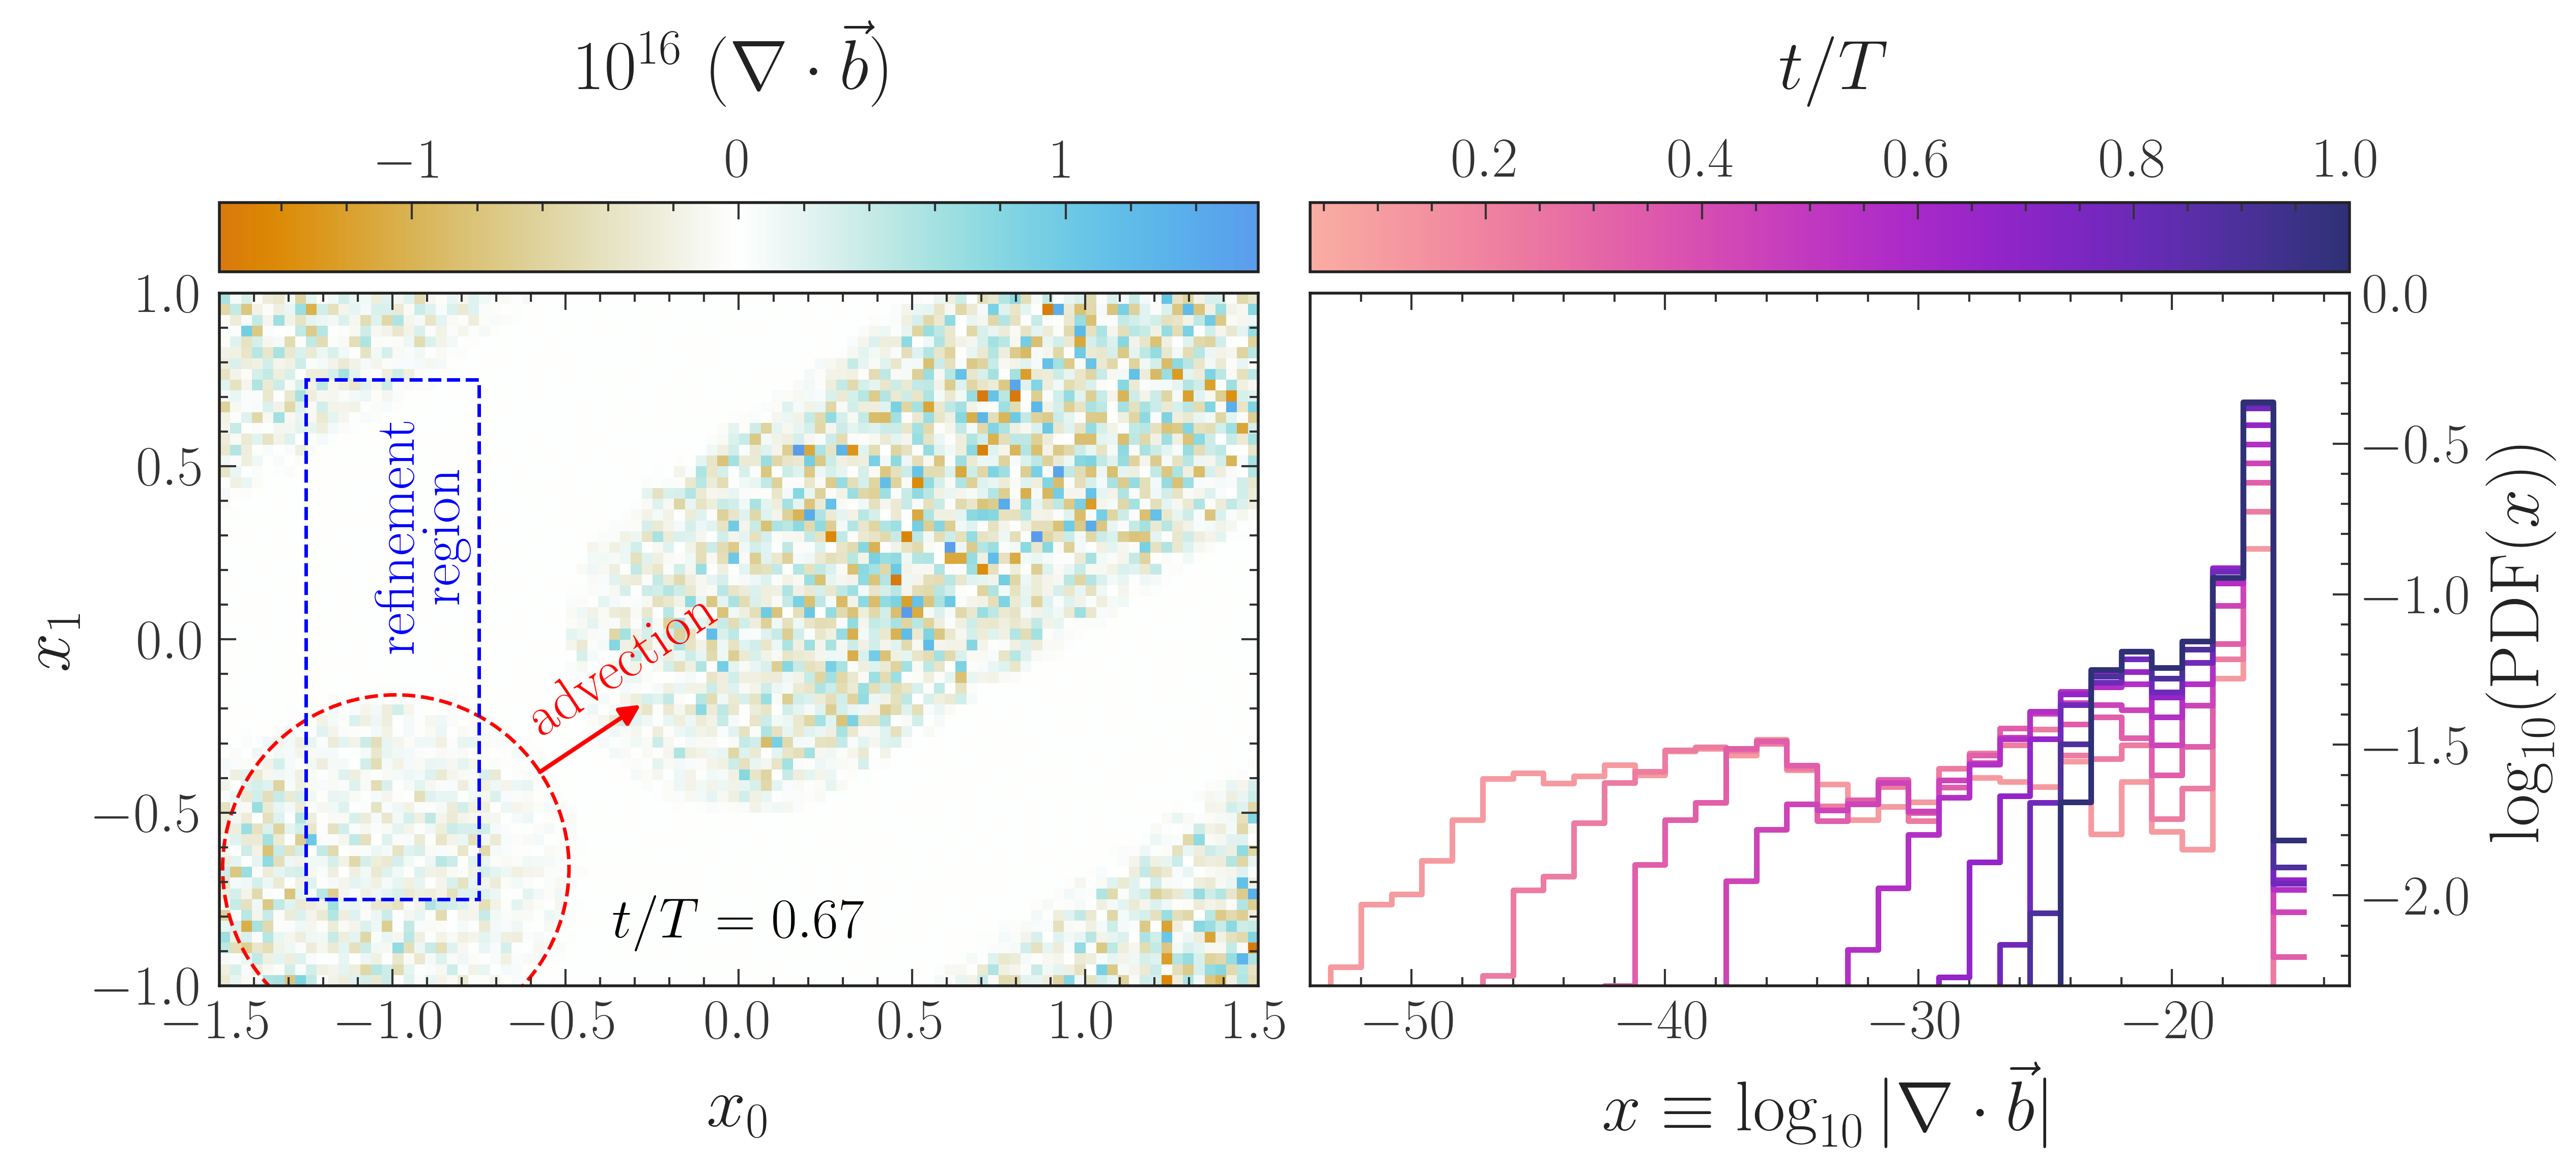
\includegraphics[width=\linewidth]{figures/quokka-mhd/results/field-loop-div-b.png}
    \caption{\DIFaddFL{Field loop advection (\mbox{%DIFAUXCMD
\citet{Gardiner08a}}\hskip0pt%DIFAUXCMD
; \sref{sec:stress-tests:field-loop}) with one level of static mesh refinement, run for a full period with our recommended scheme (Q26 compute, \mbox{%DIFAUXCMD
\citetalias{Balsara25b} }\hskip0pt%DIFAUXCMD
averaging, and PPM-EP reconstruction). The left panel shows a slice of $\nabla\cdot\mVector{b}$, at a time $t / T \approx 0.67$ where the loop is partially embedded within the refined region. The right panel shows the distribution of $\nabla\cdot\mVector{b}$ values evolving throughout the run, with colours showing time in units of the advection period $T$.}}
    \label{fig:stress-tests:field-loop}
\end{figure*}

\DIFadd{One of the most important constraints of any MHD simulation is satisfying $\nabla\cdot\mVector{b} = 0$. The CT formalism (\sref{sec:methods:mesh}) does so by construction, however, only up to numerical precision. In the presence of AMR (\mbox{%DIFAUXCMD
\cref{sec:methods:amr}}\hskip0pt%DIFAUXCMD
), interpolation and flux correction between coarse and fine levels have the potential to create regions where spurious, finite-precision-level $\nabla\cdot\mVector{b}$ could, in principle, form. Here we confirm that our implementation maintains $\nabla\cdot\mVector{b} = 0$ to numerical precision under these conditions.
}

\DIFadd{Following \mbox{%DIFAUXCMD
\citet{Gardiner08a}}\hskip0pt%DIFAUXCMD
, we set up a closed, magnetic field loop advecting across a periodic domain spanning $x_0 \in [-1.5, 1.5]$}\DIFaddend , \DIFaddbegin \DIFadd{$x_1 \in [-1, 1]$, and $x_2 \in [-0.5, 0.5]$, with a refined region offset from the loop's initial position (\mbox{%DIFAUXCMD
\cref{fig:stress-tests:field-loop} }\hskip0pt%DIFAUXCMD
annotates its location). With $\gamma = 5/3$, we initialise,
}\begin{align}
    \mVector{S}_\mathrm{c}
        = \begin{Bmatrix}
                \rho \\
                \mVector{u} \\
                p \\
                \mVector{b}
            \end{Bmatrix}
        = \begin{Bmatrix}
                1 \\
                \dfrac{1}{\sqrt{13}}\rbrac{3\,\mVectorUnit{x}_0 + 2\,\mVectorUnit{x}_1 + \mVectorUnit{x}_2} \\
                1 \\
                \dfrac{\delta b}{r}\rbrac{x_0\,\mVectorUnit{x}_1 - x_1\,\mVectorUnit{x}_0}
            \end{Bmatrix}
    ,
\end{align}
\DIFadd{where $r = \rbrac{x_0^2 + x_1^2}^{1/2}$ }\DIFaddend and
\DIFaddbegin \begin{align}
    \delta b
        = \begin{cases}
                10^{-3}
                    & , \qquad r < R \\
                0
                    & , \qquad r \geq R
            \end{cases}
    ,
\end{align}
\DIFadd{Since $\delta b \ll 1$ (magnetic pressure is far smaller than the background pressure), and $\mVector{u}$ is spatially uniform, the magnetic field loop is dynamically passive, and purely advects with the flow. We evolve this setup with radius $R = 0.5$ for one full advection period across the triply-periodic domain, $t / T = 1$. We choose to simulate at a low resolution of $96 \times 64 \times 32$ cells, and one additional AMR level, so that grid effects would be visually apparent.
}

\DIFadd{\mbox{%DIFAUXCMD
\Cref{fig:stress-tests:field-loop} }\hskip0pt%DIFAUXCMD
shows that no spurious $\nabla\cdot\mVector{b}$ is produced once the loop has entered the refined region, with $\nabla\cdot\mVector{b} \sim 10^{-16}$ (close to machine precision) both in the portion of the advection that took place on the base resolution (upper-right region of the slice panel) and once it crosses the refined region (bottom-left region). Beyond this single slice, we also show that the time-evolution of the distribution of $\nabla\cdot\mVector{b}$ values remains concentrated at the level of finite precision, rather than systematically shifting to increasingly larger values.
}

\subsection{\DIFadd{Ohmic resistivity}}
\label{sec:stress-tests:resistivity}

\begin{figure}
    \centering
    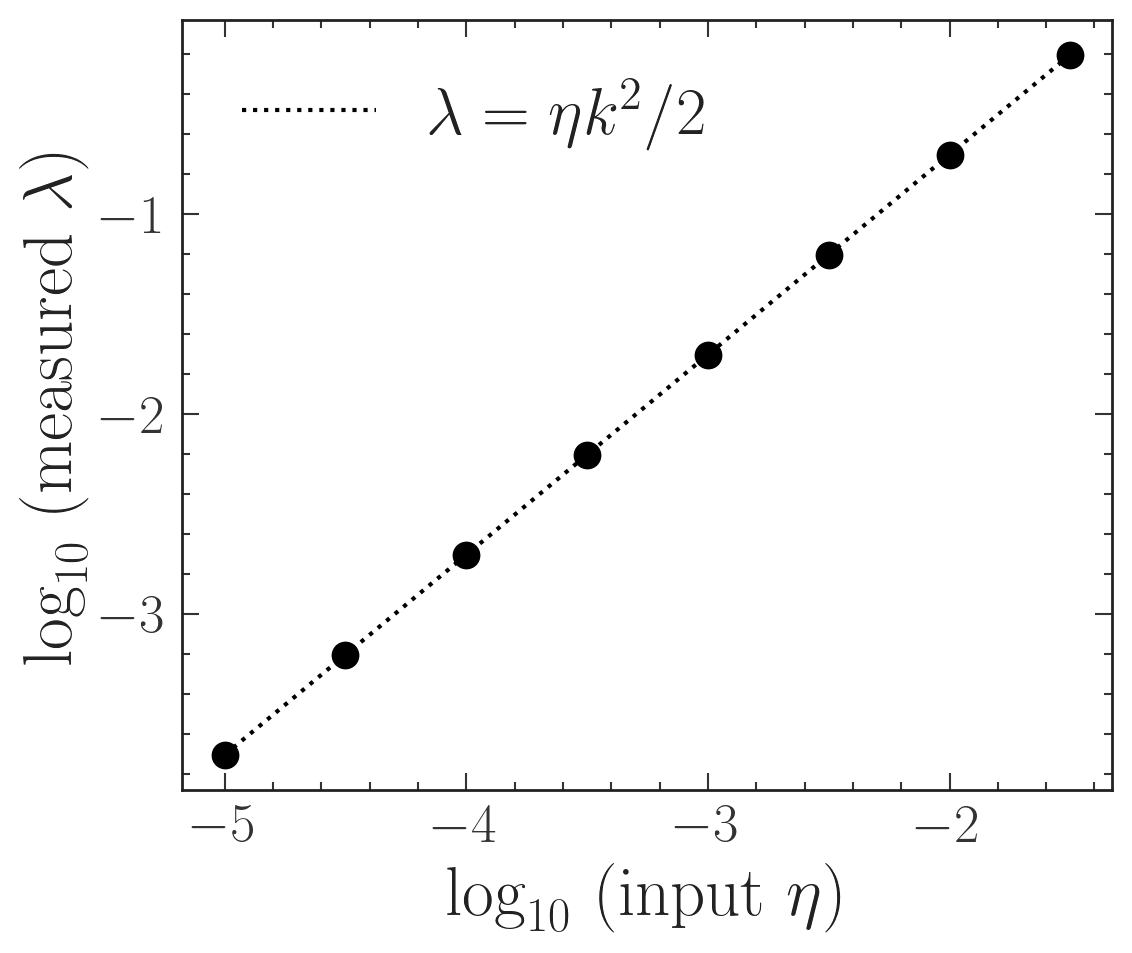
\includegraphics[width=0.65\linewidth]{figures/quokka-mhd/results/alfven-wave-linear-resistive-decay-rate.png}
    \caption{\DIFaddFL{Measured decay rate of }\DIFaddendFL the \DIFdelbeginFL \DIFdelFL{state after $3$ advection periods in }\DIFdelendFL \DIFaddbeginFL \DIFaddFL{resistively-damped Alfv\'en wave (\sref{sec:stress-tests:resistivity}) compared with }\DIFaddendFL the \DIFdelbeginFL \DIFdelFL{bottom panels. The direction of advection is shown }\DIFdelendFL \DIFaddbeginFL \DIFaddFL{input resistivity $\eta$, run }\DIFaddendFL with \DIFdelbeginFL \DIFdelFL{an arrow}\DIFdelendFL \DIFaddbeginFL \DIFaddFL{our recommended scheme (Q26 compute}\DIFaddendFL , \DIFaddbeginFL \DIFaddFL{\mbox{%DIFAUXCMD
\citetalias{Balsara25b} }\hskip0pt%DIFAUXCMD
averaging, }\DIFaddendFL and \DIFaddbeginFL \DIFaddFL{PPM-EP reconstruction) at }\DIFaddendFL a \DIFdelbeginFL \DIFdelFL{reference circle to highlight how well the vortex maintains its shape}\DIFdelendFL \DIFaddbeginFL \DIFaddFL{fixed resolution of $N=256$}\DIFaddendFL . \DIFdelbeginFL \DIFdelFL{We also indicate }\DIFdelendFL \DIFaddbeginFL \DIFaddFL{The dotted line shows }\DIFaddendFL the \DIFdelbeginFL \DIFdelFL{fraction of magnetic energy that is conserved}\DIFdelendFL \DIFaddbeginFL \DIFaddFL{analytic prediction $\lambda = \eta k^2/2$}\DIFaddendFL .}
    \DIFdelbeginFL %DIFDELCMD < \label{fig:balsara-vortex}
%DIFDELCMD < %%%
\DIFdelendFL \DIFaddbeginFL \label{fig:resistive-alfven-decay}
\DIFaddendFL \end{figure}

%DIF <  \subsection{Small-scale dynamo}
    \DIFaddbegin \DIFadd{Having thoroughly validated our recommended scheme against ideal MHD, we now validate our implementation of constant Ohmic resistivity (\sref{sec:methods:resistivity}), which makes two additions to the ideal update: a resistive correction to the EMF components (\mbox{%DIFAUXCMD
\cref{eqn:resistivity:emf-update}}\hskip0pt%DIFAUXCMD
) and a corresponding Joule-heating term that is added to the total-energy flux. We validate these steps separately.
}\DIFaddend

\DIFaddbegin \DIFadd{First, we check that a resistively-damped, linearly-polarised Alfv\'en wave decays as the analytic solution predicts. Substituting the resistive Ohm's law (\mbox{%DIFAUXCMD
\cref{eqn:resistivity:ohms-law}}\hskip0pt%DIFAUXCMD
) into the induction equation (\mbox{%DIFAUXCMD
\cref{eqn:induction:continuous}}\hskip0pt%DIFAUXCMD
) means that a wave that would ideally oscillate at $\omega_\mathrm{ideal} = c_\mathrm{A} k \cos\theta$ instead decays as $\exp\sbrac{-\lambda t}$, where
}\begin{align}
    \lambda
        = \frac{\eta k^2}{2}
    , \label{eqn:resistivity:alfven-decay}
\end{align}
\DIFadd{and oscillates at $\omega_\mathrm{real}$ (the real part of the complex frequency), where
}\begin{align}
    \omega_\mathrm{real}
        = \sqrt{\omega_\mathrm{ideal}^2 - \lambda^2}
    . \label{eqn:resistivity:alfven-frequency}
\end{align}
\DIFadd{We use the same linearly-polarised Alfv\'en wave setup as in \sref{sec:scheme-comparison:waves:alfven-linear}, run with the wave propagating grid-aligned, $\mVector{k}L/2\pi = \{1,0,0\}$, and a constant resistivity $\eta$ introduced. We run $8$ instances of this test at a fixed resolution $N = 256$, varying $\eta \in [10^{-5}, 3.16 \times 10^{-2}]$ between each simulation, using $\mathrm{CFL} = 0.3$ throughout, consistent with the 3D stability requirement discussed in \sref{sec:methods:resistivity}. \mbox{%DIFAUXCMD
\Cref{fig:resistive-alfven-decay} }\hskip0pt%DIFAUXCMD
shows that the measured decay rate matches the analytic $\lambda = \eta k^2/2$ (\mbox{%DIFAUXCMD
\cref{eqn:resistivity:alfven-decay}}\hskip0pt%DIFAUXCMD
) across the full range, confirming that the resistive EMF correction performs as expected.
}

\DIFadd{This test, however, cannot validate the Joule-heating term: a periodic domain conserves total energy regardless of whether this term is implemented correctly, so a global energy check cannot distinguish a correct implementation from a broken, or missing, one. We separately confirm that the Joule-heating term is implemented correctly, matching \mbox{%DIFAUXCMD
\cref{eqn:resistivity:current-stencil} }\hskip0pt%DIFAUXCMD
to machine precision.
}


\DIFaddend \section{Chapter Conclusions}
\label{sec:conclusions}

In this \DIFdelbegin \DIFdel{paper }\DIFdelend \DIFaddbegin \DIFadd{chapter }\DIFaddend we have implemented \DIFdelbegin \DIFdel{ideal MHD into }\textsc{\DIFdel{Quokka}}%DIFAUXCMD
\DIFdelend \DIFaddbegin \DIFadd{an MHD module, supporting both ideal and resistive (constant Ohmic) regimes, into the open-source code \quokka}\DIFaddend , extending its GPU-native radiation-hydrodynamic framework to magnetised flows. Our implementation couples to the existing Godunov finite-volume update of cell-centred state variables via a constrained transport (CT) update that stores magnetic fields on cell faces, using a staggered mesh
(see \DIFdelbegin %DIFDELCMD < \autoref{fig:schematic:grid}%%%
\DIFdelend \DIFaddbegin \DIFadd{\mbox{%DIFAUXCMD
\cref{fig:schematic:grid}}\hskip0pt%DIFAUXCMD
}\DIFaddend ) that ensures $\nabla\cdot\mVector{b} = 0$ (to numerical precision) by construction. For the fluxes on these faces, we use a\DIFaddbegin \DIFadd{n}\DIFaddend  HLLD Riemann solver with stability and low-$\mathcal{M}$ pressure fixes based on \citet{Minoshima21a} (see \DIFdelbegin %DIFDELCMD < \autoref{sec:methods:flux}%%%
\DIFdelend \DIFaddbegin \DIFadd{\sref{sec:methods:flux}}\DIFaddend ), and develop a first-order flux correction (FOFC) strategy that improves stability by detecting cells whose high-order update would produce an unphysical state and locally falling back to a more dissipative first-order update (see \DIFdelbegin %DIFDELCMD < \autoref{sec:methods:time-stepping}%%%
\DIFdelend \DIFaddbegin \DIFadd{\sref{sec:methods:time-stepping}}\DIFaddend ).

We \DIFdelbegin \DIFdel{break }\DIFdelend \DIFaddbegin \DIFadd{divide }\DIFaddend our CT scheme (see \DIFdelbegin %DIFDELCMD < \autoref{sec:methods:emf}%%%
\DIFdelend \DIFaddbegin \DIFadd{\sref{sec:methods:emf}}\DIFaddend ) up into two modular parts: (i) how the edge-centred EMFs are \DIFdelbegin \DIFdel{reconstructed }\DIFdelend \DIFaddbegin \DIFadd{computed }\DIFaddend from neighbouring face- and cell-centred data (see \DIFdelbegin %DIFDELCMD < \autoref{sec:methods:emf:reconstruction}%%%
\DIFdelend \DIFaddbegin \DIFadd{\sref{sec:methods:emf:compute}}\DIFaddend ), and (ii) how the four\DIFaddbegin \DIFadd{-quadrant}\DIFaddend  estimates for the EMF around each edge are combined into a single upwinded value (see \DIFdelbegin %DIFDELCMD < \autoref{sec:methods:emf:averaging}%%%
\DIFdelend \DIFaddbegin \DIFadd{\sref{sec:methods:emf:averaging}}\DIFaddend ). For the EMF \DIFdelbegin \DIFdel{reconstruction }\DIFdelend \DIFaddbegin \DIFadd{compute }\DIFaddend step we implemented \DIFdelbegin \DIFdel{the algorithms proposed by both }\DIFdelend \DIFaddbegin \DIFadd{two recent, state-of-the-art EMF compute schemes produced by }\DIFaddend \citetalias{Felker18a} and \citetalias{Balsara25a} (see \DIFdelbegin \DIFdel{Schematics~\ref{fig:schematic:fs18} }\DIFdelend \DIFaddbegin \DIFadd{\mbox{%DIFAUXCMD
\cref{fig:schematic:fs18} }\hskip0pt%DIFAUXCMD
}\DIFaddend and \ref{fig:schematic:b25}, respectively), \DIFdelbegin \DIFdel{alongside a new strategy introduced in this paper }\DIFdelend \DIFaddbegin \DIFadd{and, in this chapter, we also introduce a new scheme }\DIFaddend (Q26; see \DIFdelbegin \DIFdel{Schematic~\ref{fig:schematic:q26})that reconstructs EMFs from the velocities on cell faces deduced }\DIFdelend \DIFaddbegin \DIFadd{\mbox{%DIFAUXCMD
\cref{fig:schematic:q26}}\hskip0pt%DIFAUXCMD
). Our new scheme computes EMFs from face-normal velocities obtained }\DIFaddend directly from the \DIFdelbegin \DIFdel{Riemann problem solution on those faces; this }\DIFdelend \DIFaddbegin \DIFadd{flux calculation, rather than reconstructing them separately from cell centres, which }\DIFaddend reduces the number of \DIFdelbegin \DIFdel{interpolation }\DIFdelend \DIFaddbegin \DIFadd{reconstruction }\DIFaddend operations and temporary variables required \DIFdelbegin \DIFdel{to reconstruct EMFs on cell-edges}\DIFdelend \DIFaddbegin \DIFadd{for this step}\DIFaddend . We also implemented two EMF averaging \DIFdelbegin \DIFdel{strategies}\DIFdelend \DIFaddbegin \DIFadd{schemes}\DIFaddend , namely those of \citetalias{Londrillo04a} and \citetalias{Balsara25b}.

To determine which combination of these EMF \DIFdelbegin \DIFdel{reconstruction }\DIFdelend \DIFaddbegin \DIFadd{compute }\DIFaddend and EMF averaging schemes best \DIFdelbegin \DIFdel{align with }\textsc{\DIFdel{Quokka}}%DIFAUXCMD
\DIFdelend \DIFaddbegin \DIFadd{aligns with \quokka}\DIFaddend 's performance goals (see \DIFdelbegin %DIFDELCMD < \autoref{sec:intro:goals} %%%
\DIFdelend \DIFaddbegin \DIFadd{\sref{sec:intro:goals} }\DIFaddend for a discussion), we perform a rigorous and systematic comparison (\DIFdelbegin %DIFDELCMD < \autoref{sec:performance}%%%
\DIFdelend \DIFaddbegin \DIFadd{\sref{sec:scheme-comparisons}}\DIFaddend ) of the accuracy and efficiency of every combination of EMF \DIFdelbegin \DIFdel{reconstruction }\DIFdelend \DIFaddbegin \DIFadd{compute }\DIFaddend and averaging together with three \DIFdelbegin \DIFdel{interpolation }\DIFdelend \DIFaddbegin \DIFadd{reconstruction }\DIFaddend methods: piecewise linear (PLM), piecewise parabolic (PPM), and extrema-preserving PPM (PPM-EP). We test \DIFdelbegin \DIFdel{the schemes }\DIFdelend \DIFaddbegin \DIFadd{all scheme combinations of EMF compute, EMF averaging, and reconstruction method }\DIFaddend against both linear and highly-non\DIFaddbegin \DIFadd{-}\DIFaddend linear problems, and compare not only accuracy \DIFdelbegin \DIFdel{and stability but also speed }\DIFdelend \DIFaddbegin \DIFadd{but also GPU throughput }\DIFaddend and scaling. Based on \DIFdelbegin \DIFdel{this }\DIFdelend \DIFaddbegin \DIFadd{our }\DIFaddend systematic comparison, we recommend our Q26 EMF \DIFdelbegin \DIFdel{reconstruction }\DIFdelend \DIFaddbegin \DIFadd{compute }\DIFaddend scheme coupled with \DIFdelbegin \DIFdel{\mbox{%DIFAUXCMD
\citetalias{Balsara25a} }\hskip0pt%DIFAUXCMD
}\DIFdelend \DIFaddbegin \DIFadd{\mbox{%DIFAUXCMD
\citetalias{Balsara25b} }\hskip0pt%DIFAUXCMD
}\DIFaddend and PPM-EP as the default \DIFdelbegin \DIFdel{configuration for }\textsc{\DIFdel{Quokka}}%DIFAUXCMD
\DIFdel{. This combination provides the best overall balance of accuracy, stability, and GPU-efficiency across flow conditions from simple and smooth to turbulent and instability driven, and is noticeably faster than any alternatives . If better robustness is required, we recommend exchanging Q26 with \mbox{%DIFAUXCMD
\citetalias{Balsara25b}}\hskip0pt%DIFAUXCMD
, which provides improved stability at the price of being $\approx 1.3\times$ slower. We show that }\DIFdelend \DIFaddbegin \DIFadd{scheme combination for \quokka, since it provides roughly $30$--$60\%$ higher GPU throughput than the alternatives we test (\sref{sec:scheme-comparison:speed}; \mbox{%DIFAUXCMD
\cref{fig:gpu-scaling}}\hskip0pt%DIFAUXCMD
), resolves equally accurate flow dynamics as the alternatives we considered, and was one of the most stable scheme combinations at this accuracy in reconnection-dominated flows (\sref{sec:scheme-comparison:reconnection}). Finally, we further validate }\DIFaddend our recommended scheme \DIFdelbegin \DIFdel{passes a number of other standard tests , with excellent performance (see }%DIFDELCMD < \autoref{sec:tests}%%%
\DIFdelend \DIFaddbegin \DIFadd{against a broader suite of tests (\sref{sec:stress-tests}}\DIFaddend ).

\DIFdelbegin \DIFdel{The ideal MHD framework implemented in this paper provides a robust and efficient module ready for scientific use, }\DIFdelend \DIFaddbegin \DIFadd{In future work we intend to expand these capabilities further into the non-ideal MHD regime, by adding treatments of ion-neutral drift and the Hall effect.
}


\section*{\DIFadd{Chapter Acknowledgements}}

\DIFadd{We thank James R. Beattie and James Watt for many fruitful discussions that have greatly benefited this work.
}

\DIFadd{N.~K. acknowledges financial support from the Australian Government via the Australian Government Research Training Program Fee-Offset Scholarship. This work was supported by the Australian Research Council through award FL220100020 (to M.~R.~K.), }\DIFaddend and \DIFdelbegin \DIFdel{provides a platform for future extensions.
A natural next step is to incorporate explicit physical dissipation into }\textsc{\DIFdel{Quokka}}%DIFAUXCMD
\DIFdel{, including both shear and bulk viscosity in the momentum equation (as was done in \mbox{%DIFAUXCMD
\citealt{beattie2025taking}}\hskip0pt%DIFAUXCMD
)and Ohmic dissipation in the induction equation. These extensions would allow for controlled simulations of MHD turbulence, where dissipation effects directly affect the transport of energy and coupling of magnetic and velocity fields. In addition to this, we plan to implement a slow-shock stability fix in the HLLD Riemann solverto improve the stability of the Q26 reconstruction scheme when coupled to higher-order interpolation}\DIFdelend \DIFaddbegin \DIFadd{by computing resources supported by the Australian Government's National Collaborative Research Infrastructure Strategy (NCRIS), with access to Gadi at the National Computational Infrastructure and Setonix at the Pawsey Supercomputing Centre, through the National Computational Merit Allocation Scheme (award jh2). N.~K. also gratefully acknowledges access to the Marvin cluster and support from the HPC@HRZ Team and the High Performance Computing \& Analytics Lab at the University of Bonn.
}

\DIFadd{This work made use of the }\textsc{\DIFadd{AMReX}} \DIFadd{framework \mbox{%DIFAUXCMD
\citep{Zhang19b}}\hskip0pt%DIFAUXCMD
, on which \quokka~is built. We also relied on the following programming languages and software packages to analyse and produce visualisations of our simulation data: }\textsc{\DIFadd{C++}} \DIFadd{\mbox{%DIFAUXCMD
\citep{stroustrup2013cpp}}\hskip0pt%DIFAUXCMD
, }\textsc{\DIFadd{python}} \DIFadd{along with }\textsc{\DIFadd{numpy}} \DIFadd{\mbox{%DIFAUXCMD
\citep{oliphant2006guide, van2011numpy, harris2020array}}\hskip0pt%DIFAUXCMD
, }\textsc{\DIFadd{matplotlib}} \DIFadd{\mbox{%DIFAUXCMD
\citep{hunter2007matplotlib, bisong2019matplotlib}}\hskip0pt%DIFAUXCMD
, and }\textsc{\DIFadd{cython}} \DIFadd{\mbox{%DIFAUXCMD
\citep{behnel2010cython, smith2015cython}}\hskip0pt%DIFAUXCMD
. The exact MHD Riemann solver, }\textsc{\DIFadd{MHDRiemannSolver}} \DIFadd{\mbox{%DIFAUXCMD
\citep{Kriel26a}}\hskip0pt%DIFAUXCMD
, was developed by N.~K. to compute reference solutions of the shock-tube test in \mbox{%DIFAUXCMD
\cref{sec:scheme-comparison:shocks:ryu-jones}}\hskip0pt%DIFAUXCMD
}\DIFaddend .

\section{Chapter End Matter}

\subsection{A Note on Notation}
\label{sec:notation}

\DIFaddbegin \DIFadd{Throughout this chapter we work with quantities that have many different variants, are stored on different stencils, and are evaluated at different times. To express all of this information consistently, we adopt a few notational conventions that depart from standard practice, so we describe them below.
}

\DIFaddend \paragraph*{Field and index conventions.}
\DIFaddbegin

\DIFaddend We use lower-case symbols for scalar and vector fields, and upper-case symbols for collections (\eg\DIFaddbegin \DIFadd{~}\DIFaddend the state vector; see \DIFdelbegin %DIFDELCMD < \autoref{defn:state-vector}%%%
\DIFdelend \DIFaddbegin \DIFadd{\mbox{%DIFAUXCMD
\cref{eqn:state:conserved}}\hskip0pt%DIFAUXCMD
}\DIFaddend ) and for rank-2 tensors. Spatial indices $i$, $j$, and $k$ denote mesh positions: integers refer to cell centres, and half-integers to faces or edges (see \DIFdelbegin %DIFDELCMD < \autoref{fig:schematic:grid}%%%
\DIFdelend \DIFaddbegin \DIFadd{\mbox{%DIFAUXCMD
\cref{fig:schematic:grid}}\hskip0pt%DIFAUXCMD
}\DIFaddend ). Numbered subscripts indicate vector components aligned with coordinate axes\DIFdelbegin \DIFdel{; in three dimensions these }\DIFdelend \DIFaddbegin \DIFadd{, which }\DIFaddend correspond to the \DIFaddbegin \DIFadd{$x_0$, }\DIFaddend $x_1$, \DIFdelbegin \DIFdel{$x_2$, and $x_3$ directions , which follow }\DIFdelend \DIFaddbegin \DIFadd{and $x_2$ directions (following }\DIFaddend the usual right-hand rule\DIFdelbegin \DIFdel{. Sub- and superscripts are also used to indicate context-specific information.
}\DIFdelend \DIFaddbegin \DIFadd{).
}\DIFaddend

\paragraph*{Brackets and superscripts.}
\DIFaddbegin

\DIFaddend Round brackets denote grouping, \eg~$a(b+c)$. Square brackets \DIFdelbegin \DIFdel{indicate evaluation at a discrete time level}\DIFdelend \DIFaddbegin \DIFadd{serve three roles: to group a set of arguments of a function or operator, }\eg\DIFadd{~$\exp\sbrac{1 - r^2}$; grouping the indices at which a quantity is sampled, }\eg\DIFadd{~$b_0\EvalAtH{i+1/2}{j}{k}$ (see \mbox{%DIFAUXCMD
\cref{fig:schematic:grid}}\hskip0pt%DIFAUXCMD
); or, as a superscript, indicating a discrete case or instance of a quantity, either a time step}\DIFaddend , $\mVector{S}^{[n]}$ \DIFdelbegin \DIFdel{, $\mVector{S}^{[n+1/2]}$, and $\mVector{S}^{[n+1]}$}\DIFdelend \DIFaddbegin \DIFadd{(see \mbox{%DIFAUXCMD
\cref{eqn:rk1:update,eqn:rk2:update}}\hskip0pt%DIFAUXCMD
), or a specific reconstructed variant or wave type, $\varepsilon_2^{[LB]}$ and $\varepsilon_2^{[RT]}$ (see \mbox{%DIFAUXCMD
\cref{eqn:emf:ld04}}\hskip0pt%DIFAUXCMD
)}\DIFaddend . Curly brackets \DIFdelbegin \DIFdel{denote collections, such as the components of a vector}\DIFdelend \DIFaddbegin \DIFadd{serve two roles: standard mathematical set membership, }\eg\DIFadd{~$S_\mathrm{I} \in \{L, R\}$ (see \sref{sec:methods:emf:compute}); or, as a subscript, a set of quantities that are jointly referenced or combined by the enclosing operator, }\eg\DIFadd{~$\bar{u}_{\cbrac{0,1}}$ for the average of $u_0$ and $u_1$ (see \mbox{%DIFAUXCMD
\cref{eqn:emf:fs18-average}}\hskip0pt%DIFAUXCMD
)}\DIFaddend . Superscripts are \DIFdelbegin \DIFdel{used in three }\DIFdelend \DIFaddbegin \DIFadd{therefore used in two }\DIFaddend ways: (i) \DIFdelbegin \DIFdel{to indicate time levels, as above; }\DIFdelend \DIFaddbegin \DIFadd{in square brackets, to indicate either a time step or a variant, and }\DIFaddend (ii) \DIFdelbegin \DIFdel{to distinguish reconstructed variants, in which case contextual information is enclosed in curly brackets, $\varepsilon_{3}^{\cbrac{TL}}\EvalAtH{i + 1/2}{j + 1/2}{k}$ and $\varepsilon_{3}^{\cbrac{BR}}\EvalAtH{i + 1/2}{j + 1/2}{k}$ and (iii) in }\DIFdelend \DIFaddbegin \DIFadd{in }\DIFaddend the usual sense to denote powers (\DIFdelbegin \DIFdel{though this usage is rare in this paper}\DIFdelend \DIFaddbegin \DIFadd{when not enclosed by square brackets}\DIFaddend ).

\paragraph*{Directional \DIFdelbegin \DIFdel{splitting }\DIFdelend \DIFaddbegin \DIFadd{notation }\DIFaddend and interface \DIFdelbegin \DIFdel{notation}\DIFdelend \DIFaddbegin \DIFadd{labels}\DIFaddend .\DIFdelbegin %DIFDELCMD < \MBLOCKRIGHTBRACE
%DIFDELCMD < %%%
\DIFdel{Because our update is directionally split}\DIFdelend \DIFaddbegin }

\DIFadd{Because the same procedure is applied independently along each direction}\DIFaddend , we describe the \DIFdelbegin \DIFdel{algorithm }\DIFdelend \DIFaddbegin \DIFadd{scheme }\DIFaddend through the flux across the \DIFdelbegin \DIFdel{$x_1$}\DIFdelend \DIFaddbegin \DIFadd{$x_0$}\DIFaddend -oriented face; the corresponding expressions for the \DIFdelbegin \DIFdel{$x_2$}\DIFdelend \DIFaddbegin \DIFadd{$x_1$}\DIFaddend - and \DIFdelbegin \DIFdel{$x_3$}\DIFdelend \DIFaddbegin \DIFadd{$x_2$}\DIFaddend -faces follow by cyclic permutation of the $i$, $j$, and $k$ indices \DIFdelbegin \DIFdel{. For clarity}\DIFdelend \DIFaddbegin \DIFadd{(see \mbox{%DIFAUXCMD
\cref{fig:schematic:grid}}\hskip0pt%DIFAUXCMD
). For simplicity}\DIFaddend , we therefore \DIFdelbegin \DIFdel{work locally in the two-dimensional }\DIFdelend \DIFaddbegin \DIFadd{describe all schemes in the local, 2D }\DIFaddend plane spanned by \DIFdelbegin \DIFdel{$x_1$ and $x_2$}\DIFdelend \DIFaddbegin \DIFadd{$x_0$ and $x_1$}\DIFaddend .

\DIFdelbegin \DIFdel{In reconstruction, interface states are labelled as }\DIFdelend \DIFaddbegin \DIFadd{The interface states that are produced by reconstruction are labelled: }\DIFaddend left ($L$) and right ($R$), or top ($T$) and bottom ($B$). We denote side-based states by $S_\mathrm{I} \in \{L, R\}$ and $S_\mathrm{II} \in \{T, B\}$ \DIFaddbegin \DIFadd{(see \mbox{%DIFAUXCMD
\cref{fig:schematic:b-common}}\hskip0pt%DIFAUXCMD
)}\DIFaddend , and quadrant-based states either as single-sided labels $Q_\mathrm{I} \in \{T, R, B, L\}$ (\DIFdelbegin \DIFdel{for example, face-centred quantities reconstructed to a cell edge; see }%DIFDELCMD < \autoref{fig:schematic:q26}%%%
\DIFdelend \DIFaddbegin \DIFadd{see \mbox{%DIFAUXCMD
\cref{fig:schematic:q26}}\hskip0pt%DIFAUXCMD
}\DIFaddend ), or as corner combinations \DIFdelbegin \DIFdel{$Q_\mathrm{II} \in \{TL, TR, BR, BL\}$ (for example, cell-centred quantities reconstructed to a cell edge; see }%DIFDELCMD < \autoref{fig:schematic:fs18}%%%
\DIFdelend \DIFaddbegin \DIFadd{$Q_\mathrm{II} \in \{LB, RB, LT, RT\}$ (see \mbox{%DIFAUXCMD
\cref{fig:schematic:fs18}}\hskip0pt%DIFAUXCMD
}\DIFaddend ). When necessary, we explicitly indicate \DIFdelbegin \DIFdel{reconstruction order or direction, for example $u_1^{\{Q_\mathrm{II}: x_1 x_2\}}$ and $u_1^{\{Q_\mathrm{II}: x_2 x_1\}}$}\DIFdelend \DIFaddbegin \DIFadd{the order of reconstruction steps, }\eg\DIFadd{~$u_0^{[Q_\mathrm{II}: x_0 x_1]}$ and $u_0^{[Q_\mathrm{II}: x_1 x_0]}$}\DIFaddend .

    \chapter{Conclusion}

\section{Thesis Summary}

In this thesis I have used direct numerical simulations to study the attractor states of small-scale dynamos (SSDs), and quantified how compressibility shifts attractor properties. While the results in \S\ref{chapter:ssd-exp} and \S\ref{chapter:ssd-nl} have broader implications for SSDs in $\mathrm{Pm} \geq 1$ plasmas, I use galactic magnetism as the lens for this summary, and refer the reader back to the concluding sections of each paper-chapter for a wider-scope discussion and summary of results.

In \S\ref{chapter:ssd-exp}, I explored how large-scale magnetic structure could be generated in young galaxies, long before large-scale coherence is usually expected to develop. Using periodic-box simulations of controlled and isolated SSD amplification, I quantified how compressive turbulence modifies the magnetic structures produced by SSD action. A key challenge of this process was that several measurements of field-line morphology are sensitive to dissipation and therefore to numerical resolution. To overcome this, I developed a statistical framework to extract attractor properties that give a robust, resolution-independent picture of the kinematic phase. Using this framework, I ran the most comprehensive suite of $ \mathrm{Pm} \geq 1 $ SSD simulations to date, spanning a wide range of plasma conditions, from viscous and smooth subsonic flows through to turbulent, highly supersonic, shock-dominated flow regimes. This allowed me to isolate how shocks and compressive modes modify the characteristic magnetic length scales. For galactic magnetism, the key takeaway is that while compressibility can shift the magnetic correlation scale to much larger values than incompressible SSD theory predicts, it does not by itself explain the $\sim \mathrm{kpc}$ coherence inferred in young galaxies. Instead, compressive turbulence provides a natural pathway to generate $\sim \mathrm{pc}$ fields, which must be further organised to system scales by other system-level processes.

In \S\ref{chapter:ssd-nl}, I turned to the more dynamically relevant, nonlinear stage of SSD evolution. In this regime I showed that magnetic amplification, which is intrinsically transient\footnote{
    This phase mediates the transition from the kinematic SSD attractor, where the flow is effectively quasi-hydrodynamic (only kinetic stresses affect the dynamics), to a maintained MHD regime in which the dynamics are regulated by both magnetic and kinetic stresses.
}, becomes liberated from dissipation regulated effects. In highly compressible turbulence this transient phase is difficult to identify because stochastic fluctuations obfuscate the underlying trend. To separate the underlying evolution from this variability, I developed a hierarchical Bayesian framework that couples many repeated experiments of the same setup. With this approach, I showed that the fraction of the turbulent energy injection converted into magnetic energy is approximately constant across all turbulent regimes, and is consistent with the efficiency during the kinematic phase. An immediate consequence of this is an as-yet unexplained universality in the duration of nonlinear growth when measured in turbulent eddy turnover times. In the context of galaxy evolution, this implies that even the nonlinear SSD can re-establish a maintained magneto-hydrodynamic (MHD) state on a relatively short dynamical timescale following merger- or fly-by-driven disruption.

In both \S\ref{chapter:ssd-exp} and \S\ref{chapter:ssd-nl}, I have deliberately explored SSD physics in isolation. This was necessary to concentrate numerical resolution on the inertial and resistive scales that control SSD amplification, and to develop statistical tools that extract robust measurements from the stochastic processes at play. Galactic magnetism, however, ultimately requires system-scale dynamics. If compressive turbulence in young, rapidly evolving galaxies provides a natural route to generating a larger-scale seed field early, then the remaining step is to identify which global processes subsequently act on that seed to build the $\sim \mathrm{kpc}$ coherence we see. Answering this requires simulations that resolve \textit{both} the SSD-scale physics and \textit{also} the larger-scale environment that organises the field. This is challenging with current CPU-based codes, but becomes increasingly feasible on modern GPU-accelerated supercomputers, especially using codes like \textsc{Quokka}, which were designed architecturally from the outset for these hardware capabilities. To this end, in \S\ref{chapter:quokka} I contributed to the development of the new radiation-MHD code \textsc{Quokka}, and implemented a new constrained-transport ideal-MHD module that maintains $\nabla\cdot\mVector{b} = 0$ to numerical precision by construction. I both implemented a number of existing state-of-the-art schemes and introduced a new approach in the paper, which proved to be the best scheme for the performance requirements of \textsc{Quokka}. The MHD module in \textsc{Quokka} now enables me and others to explore the next questions about galactic magnetism, which will require resolution sufficient to capture SSD amplification while simultaneously resolving the system-scale mechanisms that can organise the resulting seed field. In the following section I will highlight some of these questions.

\section{Future Work}

The ideal-MHD module that I implemented in \textsc{Quokka} has already been put to work in two projects I am involved with. One was recently awarded over a million node hours on \textsc{Frontier} and will run one of the highest-resolution isolated galaxy simulations to-date, with the goal of exploring the phase structure and properties of galactic winds. The other project focuses on determining what sets the magnetic field reversal scale in Milky Way-like galaxies. Moreover, building on the work in this thesis, I plan to use \textsc{Quokka} both to pursue scientific questions and to extend its MHD capabilities. Below I briefly outline these directions and the code developments required to enable them.

\subsection{The Saturation of the Small Scale Dynamo}

The simulations in \S\ref{chapter:ssd-exp} and \S\ref{chapter:ssd-nl} established robust attractor properties of the kinematic and nonlinear SSD, including resolution-independent morphology and a universal nonlinear growth efficiency (through the lens of turbulent eddy turnover times). Across the parameter space explored, I did not find evidence that magnetic dissipation altered the qualitative flow regime; however, my simulations were confined to modest $\mathrm{Re}$ and $\mathrm{Rm}$, where dissipation remained dynamically important and the kinematic phase was explicitly Ohmic-limited. Most astrophysical plasmas are in the $\mathrm{Rm} \gg 1$ regime, though, where dissipation is expected to become confined to increasingly thin current sheets, with magnetic energy redistributed through intermittent structures that can become unstable to tearing \citep{loureiro2017role, galishnikova2022tearing, beattie2025spectrum}. It therefore remains unclear whether the SSD approaches a dissipation-independent attractor in this $\mathrm{Rm}$ limit, or whether the maintained MHD state continues to depend on microphysical scales. To address this, I will extend \textsc{Quokka} beyond the ideal-MHD regime by implementing explicit (shear and bulk) viscosity together with Ohmic resistivity, enabling controlled variation of $\mathrm{Pm}$ and allowing the physical dissipation scale to be set and systematically pushed to smaller values while remaining resolved (as was done in this thesis). Combined with the GPU-native performance of \textsc{Quokka}, this will make substantially higher effective $\mathrm{Re}$ and $\mathrm{Rm}$ attainable than were accessible in this thesis \citep{ji2022magnetic}, and will allow a direct test of whether tearing-mediated dynamics begin to regulate saturation as current sheets become sufficiently thin. The goal is to determine how the magnetic and kinetic energy spectra, and the maintained field geometry, evolve through this transition, and whether the nonlinear SSD converges toward an asymptotic configuration.

\subsection{Magnetic Field Line Curvature}

High-energy cosmic rays (CRs) are observed to isotropise efficiently, and this has been hypothesised to be a consequence of the geometry of the magnetic field lines that thread the ISM. In these environments, CRs stream along field lines and scatter when they encounter curvature events on scales comparable to their gyroradius \citep{kempski2023cosmic, Lemoine2023_field_reversal_CR_transport}. A simple criterion for this process relies on the empirical relation $\kappa \propto b^{1/2}$ between magnetic field strength $b \equiv (\mVector{b}\cdot\mVector{b})^{1/2}$ and line curvature $\kappa = |(\mVectorUnit{b}\cdot\nabla)\mVectorUnit{b}|$. In \S\ref{chapter:ssd-exp}, I showed that this scaling emerges naturally during the kinematic phase of the SSD, consistent with earlier theoretical arguments by \citet{schekochihin2004simulations}, which showed that the quantity $b \kappa^{\alpha}$ evolves according to
\begin{align}
    \mDDFrac{\ln(b \kappa^\alpha)}{t}
        = \frac{1}{b}\mDDFrac{b}{t} + \frac{\alpha}{\kappa}\mDDFrac{\kappa}{t}
        = \rbrac{
                \alpha (\mVectorUnit{\kappa}\otimes\mVectorUnit{\kappa})
                + (1 - 2\alpha) (\mVectorUnit{b}\otimes\mVectorUnit{b})
                - \mTensor{I}
            }:\nabla\otimes\mVector{u},
\end{align}
with turbulent plasmas organising toward $\alpha = 1/2$. This behaviour has been seen across a wide range of magnetised systems: from incompressible SSDs \citep{schekochihin2004simulations}, mildly compressible maintained MHD states \citep{yuen2020curvature}, the Solar wind \citep{huang2020observations, bandyopadhyay2020situ, hu2025interplanetary}, and the Earth's magnetosheath \citep{ji2022curvature}. The ubiquity of this result suggests that the curvature distribution reflects a universal geometric constraint of magnetised flows. However, its origin remains unclear, and it is not known how robust the $\kappa \propto b^{1/2}$ coupling is once compressibility is important. In \S\ref{chapter:ssd-exp}, I found that increasing compressibility weakens this dependence, indicating that shocks and compressive modes modify the geometric relationship between field strength and curvature even during the kinematic phase. Understanding what sets this deviation requires a more detailed investigation of the curvature statistics and their connection to the underlying flow structures. I therefore plan to quantify the curvature distribution and its coupling to field strength in the nonlinear and high-$\mathrm{Rm}$ regimes accessible with \textsc{Quokka}, and to assess how these changes in magnetic geometry impact CR scattering and transport.

\subsection{The Journey From Small to Large Scale Dynamos During Galaxy Mergers}

Galaxy mergers are a setting in which SSDs and large-scale dynamos can operate in sequence. Merger-driven turbulence rapidly amplifies magnetic energy through SSD action, while the post-merger remnant introduces rotation, shear, and stratification that can organise fluctuating fields into large-scale coherence. Existing numerical studies already explore aspects of this scenario, but they largely capture different parts of the problem. Tall-box simulations \citep[\eg][]{gent2023transition} follow mean-field growth in controlled domains and show that stochastic fluctuations can slow the emergence of coherence, but their restricted geometry limits the large-scale modes that can grow, and necessarily ignore topological constraints that can only be captured in simulations including full galactic discs. Conversely, full galaxy merger simulations \citep[\eg][]{whittingham2021impact, whittingham2023impact} resolve efficient SSD amplification in the dense, turbulent central remnant, and show that differential rotation spreads magnetic energy across the disc post-merger, but their resolution is insufficient to follow the subsequent organisation into a true large-scale dynamo. My goal is to bridge these approaches using \textsc{Quokka} in an intermediate setup: two isolated galaxies (free of cluster-scale forcing) simulated at sufficient resolution to capture SSD amplification while retaining the full galactic dynamics required for large-scale organisation. This class of setup has been used extensively to study galaxy formation, but, to the best of my knowledge, has not been used to quantify dynamo action across the transition from SSD to LSD dominated dynamics. With GPU-accelerated performance, this becomes a tractable route to measure how quickly, and by which mechanisms, merger-driven SSD fields transition into coherent, system-scale structure in the post-merger remnant.


    \clearpage
    \renewcommand{\bibsection}{%
      \chapter*{References}%
      \addcontentsline{toc}{chapter}{References}%
    }
    \bibliographystyle{header/mnras}
    \begin{thebibliography}{}
\makeatletter
\relax
\def\mn@urlcharsother{\let\do\@makeother \do\$\do\&\do\#\do\^\do\_\do\%\do\~}
\def\mn@doi{\begingroup\mn@urlcharsother \@ifnextchar [ {\mn@doi@}
  {\mn@doi@[]}}
\def\mn@doi@[#1]#2{\def\@tempa{#1}\ifx\@tempa\@empty \href
  {http://dx.doi.org/#2} {doi:#2}\else \href {http://dx.doi.org/#2} {#1}\fi
  \endgroup}
\def\mn@eprint#1#2{\mn@eprint@#1:#2::\@nil}
\def\mn@eprint@arXiv#1{\href {http://arxiv.org/abs/#1} {{\tt arXiv:#1}}}
\def\mn@eprint@dblp#1{\href {http://dblp.uni-trier.de/rec/bibtex/#1.xml}
  {dblp:#1}}
\def\mn@eprint@#1:#2:#3:#4\@nil{\def\@tempa {#1}\def\@tempb {#2}\def\@tempc
  {#3}\ifx \@tempc \@empty \let \@tempc \@tempb \let \@tempb \@tempa \fi \ifx
  \@tempb \@empty \def\@tempb {arXiv}\fi \@ifundefined
  {mn@eprint@\@tempb}{\@tempb:\@tempc}{\expandafter \expandafter \csname
  mn@eprint@\@tempb\endcsname \expandafter{\@tempc}}}

\bibitem[\protect\citeauthoryear{{Alves}, {Combes}, {Ferrara}, {Forveille}  \&
  {Shore}}{{Alves} et~al.}{2016}]{collaboration2015planck}
{Alves} J.,  {Combes} F.,  {Ferrara} A.,  {Forveille} T.,   {Shore} S.,  2016,
  \mn@doi [\aap] {10.1051/0004-6361/201629543}, \href
  {https://ui.adsabs.harvard.edu/abs/2016A&A...594E...1A} {594, E1}

\bibitem[\protect\citeauthoryear{Andersson, Lazarian  \&
  Vaillancourt}{Andersson et~al.}{2015}]{andersson2015interstellar}
Andersson B.,  Lazarian A.,   Vaillancourt J.~E.,  2015, Annual Review of
  Astronomy and Astrophysics, 53, 501

\bibitem[\protect\citeauthoryear{Archontis, Dorch  \& Nordlund}{Archontis
  et~al.}{2003}]{archontis2003numerical}
Archontis V.,  Dorch S. B.~F.,   Nordlund {\AA}.,  2003, Astronomy \&
  Astrophysics, 397, 393

\bibitem[\protect\citeauthoryear{Attia, Teyssier, Katz, Kimm, Martin-Alvarez,
  Ocvirk  \& Rosdahl}{Attia et~al.}{2021}]{attia2021cosmological}
Attia M.,  Teyssier R.,  Katz H.,  Kimm T.,  Martin-Alvarez S.,  Ocvirk P.,
  Rosdahl J.,  2021, Monthly Notices of the Royal Astronomical Society, 504,
  2346

\bibitem[\protect\citeauthoryear{Bacchini, Fraternali, Iorio, Pezzulli, Marasco
   \& Nipoti}{Bacchini et~al.}{2020}]{bacchini2020evidence}
Bacchini C.,  Fraternali F.,  Iorio G.,  Pezzulli G.,  Marasco A.,   Nipoti C.,
   2020, Astronomy \& Astrophysics, 641, A70

\bibitem[\protect\citeauthoryear{{Balsara}}{{Balsara}}{2001}]{Balsara01a}
{Balsara} D.~S.,  2001, \mn@doi [\jcp] {10.1006/jcph.2001.6917}, \href
  {https://ui.adsabs.harvard.edu/abs/2001JCoPh.174..614B} {174, 614}

\bibitem[\protect\citeauthoryear{{Balsara}}{{Balsara}}{2004}]{Balsara04a}
{Balsara} D.~S.,  2004, \mn@doi [\apjs] {10.1086/381377}, \href
  {https://ui.adsabs.harvard.edu/abs/2004ApJS..151..149B} {151, 149}

\DIFaddbegin \bibitem[\protect\citeauthoryear{Balsara \& Spicer}{Balsara \&
  Spicer}{1999}]{BalsaraSpicer99a}
\DIFadd{Balsara D.~S.,  Spicer D.~S.,  1999, }\mn@doi [Journal of Computational Physics] {10.1006/jcph.1998.6153}\DIFadd{, 149, 270
}

\DIFaddend \bibitem[\protect\citeauthoryear{{Balsara}, {Bhoriya}  \& {Shu}}{{Balsara}
  et~al.}{2025a}]{Balsara25b}
{Balsara} D.~S.,  {Bhoriya} D.,   {Shu} C.-W.,  2025a, \mn@doi [Communications
  on Applied Mathematics and Computation] {10.1007/s42967-025-00517-y}, \href
  {https://ui.adsabs.harvard.edu/abs/2025arXiv250622312B/abstract} {7,
  Balsara2025}

\bibitem[\protect\citeauthoryear{{Balsara}, {Bhoriya}, {Singh}, {Kumar},
  {K{\"a}ppeli}  \& {Gatti}}{{Balsara} et~al.}{2025b}]{Balsara25a}
{Balsara} D.~S.,  {Bhoriya} D.,  {Singh} C.,  {Kumar} H.,  {K{\"a}ppeli} R.,
  {Gatti} F.,  2025b, \mn@doi [\apj] {10.3847/1538-4357/ade397}, \href
  {https://ui.adsabs.harvard.edu/abs/2025ApJ...988..134B} {988, 134}

\bibitem[\protect\citeauthoryear{Bandyopadhyay et~al.,}{Bandyopadhyay
  et~al.}{2020}]{bandyopadhyay2020situ}
Bandyopadhyay R.,  et~al., 2020, The Astrophysical Journal Letters, 893, L25

\bibitem[\protect\citeauthoryear{Barenblatt, Chorin  \&
  Prostokishin}{Barenblatt et~al.}{1997}]{barenblatt1997scaling}
Barenblatt G.,  Chorin A.,   Prostokishin V.,  1997, \mn@doi [Applied Mechanics
  Reviews] {10.1115/1.3101726}, 50, 413

\bibitem[\protect\citeauthoryear{Basu, Mao, Kepley, Robishaw, Zweibel  \&
  Gallagher~III}{Basu et~al.}{2017}]{basu2017detection}
Basu A.,  Mao S.,  Kepley A.~A.,  Robishaw T.,  Zweibel E.~G.,   Gallagher~III
  J.~S.,  2017, Monthly Notices of the Royal Astronomical Society, 464, 1003

\bibitem[\protect\citeauthoryear{Beattie \& Federrath}{Beattie \&
  Federrath}{2020}]{beattie2020filaments}
Beattie J.~R.,  Federrath C.,  2020, Monthly Notices of the Royal Astronomical
  Society, 492, 668

\bibitem[\protect\citeauthoryear{{Beattie}, {Federrath}  \& {Seta}}{{Beattie}
  et~al.}{2020}]{Beattie2020_ansotropic_shocks}
{Beattie} J.~R.,  {Federrath} C.,   {Seta} A.,  2020, \mn@doi [\mnras] {10.1093/mnras/staa2257}, \href
  {https://ui.adsabs.harvard.edu/abs/2020MNRAS.498.1593B} {498, 1593}

\bibitem[\protect\citeauthoryear{{Beattie}, {Mocz}, {Federrath}  \&
  {Klessen}}{{Beattie} et~al.}{2021}]{Beattie2021_multi_shock_model}
{Beattie} J.~R.,  {Mocz} P.,  {Federrath} C.,   {Klessen} R.~S.,  2021, \mn@doi [\mnras] {10.1093/mnras/stab1037}, \href
  {https://ui.adsabs.harvard.edu/abs/2021MNRAS.504.4354B} {504, 4354}

\bibitem[\protect\citeauthoryear{{Beattie}, {Mocz}, {Federrath}  \&
  {Klessen}}{{Beattie} et~al.}{2022}]{Beattie2022_spdf}
{Beattie} J.~R.,  {Mocz} P.,  {Federrath} C.,   {Klessen} R.~S.,  2022, \mn@doi [\mnras] {10.1093/mnras/stac3005}, \href
  {https://ui.adsabs.harvard.edu/abs/2022MNRAS.517.5003B} {517, 5003}

\bibitem[\protect\citeauthoryear{{Beattie}, {Federrath}, {Kriel}, {Hew}  \&
  {Bhattacharjee}}{{Beattie} et~al.}{2023a}]{beattie2023bulk}
{Beattie} J.~R.,  {Federrath} C.,  {Kriel} N.,  {Hew} J. K.~J.,
  {Bhattacharjee} A.,  2023a, \mn@doi [arXiv e-prints] {10.48550/arXiv.2312.03984}, \href
  {https://ui.adsabs.harvard.edu/abs/2023arXiv231203984B} {p. arXiv:2312.03984}

\bibitem[\protect\citeauthoryear{{Beattie}, {Federrath}, {Kriel}, {Mocz}  \&
  {Seta}}{{Beattie} et~al.}{2023b}]{beattie2022growth}
{Beattie} J.~R.,  {Federrath} C.,  {Kriel} N.,  {Mocz} P.,   {Seta} A.,  2023b,
  \mn@doi [\mnras] {10.1093/mnras/stad1863}, \href
  {https://ui.adsabs.harvard.edu/abs/2023MNRAS.524.3201B} {524, 3201}

\bibitem[\protect\citeauthoryear{{Beattie}, {Federrath}, {Klessen}, {Cielo}  \&
  {Bhattacharjee}}{{Beattie} et~al.}{2024}]{Beattie2024_10k_MHD}
{Beattie} J.~R.,  {Federrath} C.,  {Klessen} R.~S.,  {Cielo} S.,
  {Bhattacharjee} A.,  2024, \mn@doi [arXiv e-prints] {10.48550/arXiv.2405.16626}, \href
  {https://ui.adsabs.harvard.edu/abs/2024arXiv240516626B} {p. arXiv:2405.16626}

\bibitem[\protect\citeauthoryear{{Beattie}, {Federrath}, {Klessen}, {Cielo}  \&
  {Bhattacharjee}}{{Beattie} et~al.}{2025a}]{Beattie2025_nature_astronomy}
{Beattie} J.~R.,  {Federrath} C.,  {Klessen} R.~S.,  {Cielo} S.,
  {Bhattacharjee} A.,  2025a, \mn@doi [Nature Astronomy] {10.1038/s41550-025-02551-5}, \href
  {https://ui.adsabs.harvard.edu/abs/2025NatAs.tmp..114B} {}

\bibitem[\protect\citeauthoryear{Beattie, Federrath, Klessen, Cielo  \&
  Bhattacharjee}{Beattie et~al.}{2025b}]{beattie2025spectrum}
Beattie J.~R.,  Federrath C.,  Klessen R.~S.,  Cielo S.,   Bhattacharjee A.,
  2025b, Nature Astronomy, pp 1--11

\bibitem[\protect\citeauthoryear{Beattie, Federrath, Kriel, Hew  \&
  Bhattacharjee}{Beattie et~al.}{2025c}]{beattie2025taking}
Beattie J.~R.,  Federrath C.,  Kriel N.,  Hew J. K.~J.,   Bhattacharjee A.,
  2025c, Monthly Notices of the Royal Astronomical Society, p. staf1318

\bibitem[\protect\citeauthoryear{Beck \& Krause}{Beck \&
  Krause}{2005}]{beck2005revised}
Beck R.,  Krause M.,  2005, Astronomische Nachrichten: Astronomical Notes, 326,
  414

\bibitem[\protect\citeauthoryear{Beck, Chamandy, Elson  \& Blackman}{Beck
  et~al.}{2019}]{beck2019synthesizing}
Beck R.,  Chamandy L.,  Elson E.,   Blackman E.~G.,  2019, Galaxies, 8, 4

\bibitem[\protect\citeauthoryear{Behnel, Bradshaw, Citro, Dalcin, Seljebotn  \&
  Smith}{Behnel et~al.}{2010}]{behnel2010cython}
Behnel S.,  Bradshaw R.,  Citro C.,  Dalcin L.,  Seljebotn D.~S.,   Smith K.,
  2010, Computing in Science \& Engineering, 13, 31

\bibitem[\protect\citeauthoryear{Belfiori et~al.,}{Belfiori
  et~al.}{2025}]{belfiori2025dust}
Belfiori D.,  et~al., 2025, Astronomy \& Astrophysics, 697, A24

\bibitem[\protect\citeauthoryear{Beresnyak}{Beresnyak}{2012}]{beresnyak2012universal}
Beresnyak A.,  2012, Physical Review Letters, 108, 035002

\bibitem[\protect\citeauthoryear{{Berger} \& {Colella}}{{Berger} \&
  {Colella}}{1989}]{Berger89a}
{Berger} M.~J.,  {Colella} P.,  1989, \mn@doi [\jcp] {10.1016/0021-9991(89)90035-1}, \href
  {https://ui.adsabs.harvard.edu/abs/1989JCoPh..82...64B} {82, 64}

\bibitem[\protect\citeauthoryear{{Berger} \& {Oliger}}{{Berger} \&
  {Oliger}}{1984}]{Berger84a}
{Berger} M.~J.,  {Oliger} J.,  1984, \mn@doi [\jcp] {10.1016/0021-9991(84)90073-1}, \href
  {https://ui.adsabs.harvard.edu/abs/1984JCoPh..53..484B} {53, 484}

\bibitem[\protect\citeauthoryear{Berlok \& Pfrommer}{Berlok \&
  Pfrommer}{2019}]{berlok2019impact}
Berlok T.,  Pfrommer C.,  2019, Monthly Notices of the Royal Astronomical
  Society, 489, 3368

\bibitem[\protect\citeauthoryear{Bernet, Miniati, Lilly, Kronberg  \&
  Dessauges-Zavadsky}{Bernet et~al.}{2008}]{bernet2008strong}
Bernet M.~L.,  Miniati F.,  Lilly S.~J.,  Kronberg P.~P.,   Dessauges-Zavadsky
  M.,  2008, Nature, 454, 302

\bibitem[\protect\citeauthoryear{Bhat, Subramanian  \& Brandenburg}{Bhat
  et~al.}{2016}]{bhat2016unified}
Bhat P.,  Subramanian K.,   Brandenburg A.,  2016, Monthly Notices of the Royal
  Astronomical Society, 461, 240

\bibitem[\protect\citeauthoryear{Bian \& Aluie}{Bian \&
  Aluie}{2019}]{bian2019decoupled}
Bian X.,  Aluie H.,  2019, Physical review letters, 122, 135101

\bibitem[\protect\citeauthoryear{Biermann}{Biermann}{1950}]{biermann1950ursprung}
Biermann L.,  1950, Zeitschrift Naturforschung Teil A, 5, 65

\bibitem[\protect\citeauthoryear{Birnboim \& Dekel}{Birnboim \&
  Dekel}{2003}]{birnboim2003virial}
Birnboim Y.,  Dekel A.,  2003, Monthly Notices of the Royal Astronomical
  Society, 345, 349

\bibitem[\protect\citeauthoryear{Bisong \& Bisong}{Bisong \&
  Bisong}{2019}]{bisong2019matplotlib}
Bisong E.,  Bisong E.,  2019, Building Machine Learning and Deep Learning
  Models on Google Cloud Platform: A Comprehensive Guide for Beginners, pp
  151--165

\bibitem[\protect\citeauthoryear{Boldyrev \& Cattaneo}{Boldyrev \&
  Cattaneo}{2004}]{boldyrev2004magnetic}
Boldyrev S.,  Cattaneo F.,  2004, Physical Review Letters, 92, 144501

\bibitem[\protect\citeauthoryear{Borlaff et~al.,}{Borlaff
  et~al.}{2021}]{borlaff2021extragalactic}
Borlaff A.~S.,  et~al., 2021, The Astrophysical Journal, 921, 128

\bibitem[\protect\citeauthoryear{Bott et~al.,}{Bott
  et~al.}{2021a}]{bott2021time}
Bott A.~F.,  et~al., 2021a, Proceedings of the National Academy of Sciences,
  118

\bibitem[\protect\citeauthoryear{{Bott} et~al.,}{{Bott}
  et~al.}{2021b}]{Bott2021_time_resolved_lab_dynamo}
{Bott} A. F.~A.,  et~al., 2021b, \mn@doi [Proceedings of the National Academy
  of Science] {10.1073/pnas.2015729118}, \href
  {https://ui.adsabs.harvard.edu/abs/2021PNAS..11815729B} {118, e2015729118}

\bibitem[\protect\citeauthoryear{{Bott} et~al.,}{{Bott}
  et~al.}{2021c}]{Bott2021_supersonic_dynamo_in_lab}
{Bott} A.~F.~A.,  et~al., 2021c, \mn@doi [\prl] {10.1103/PhysRevLett.127.175002}, \href
  {https://ui.adsabs.harvard.edu/abs/2021PhRvL.127q5002B} {127, 175002}

\bibitem[\protect\citeauthoryear{Bott et~al.,}{Bott
  et~al.}{2022}]{bott2022insensitivity}
Bott A.,  et~al., 2022, Matter and Radiation at Extremes, 7

\bibitem[\protect\citeauthoryear{Bouchut, Klingenberg  \& Waagan}{Bouchut
  et~al.}{2007}]{bouchut2007multiwave}
Bouchut F.,  Klingenberg C.,   Waagan K.,  2007, Numerische Mathematik, 108, 7

\bibitem[\protect\citeauthoryear{Bouchut, Klingenberg  \& Waagan}{Bouchut
  et~al.}{2010}]{bouchut2010multiwave}
Bouchut F.,  Klingenberg C.,   Waagan K.,  2010, Numerische Mathematik, 115,
  647

\bibitem[\protect\citeauthoryear{Bovino, Schleicher  \& Schober}{Bovino
  et~al.}{2013}]{bovino2013turbulent}
Bovino S.,  Schleicher D.~R.,   Schober J.,  2013, New Journal of Physics, 15,
  013055

\DIFaddbegin \bibitem[\protect\citeauthoryear{Braginskii}{Braginskii}{1965}]{braginskii1965transport}
\DIFadd{Braginskii S.~I.,  1965, Reviews of Plasma Physics, 1, 205
}

\DIFaddend \bibitem[\protect\citeauthoryear{Brandenburg \& Banerjee}{Brandenburg \&
  Banerjee}{2025}]{brandenburg2025turbulent}
Brandenburg A.,  Banerjee A.,  2025, Journal of Plasma Physics, 91, E5

\bibitem[\protect\citeauthoryear{{Brandenburg} \& {Dobler}}{{Brandenburg} \&
  {Dobler}}{2002}]{Brandenburg02a}
{Brandenburg} A.,  {Dobler} W.,  2002, \mn@doi [Computer Physics
  Communications] {10.1016/S0010-4655(02)00334-X}, \href
  {http://adsabs.harvard.edu/abs/2002CoPhC.147..471B} {147, 471}

\bibitem[\protect\citeauthoryear{Brandenburg \& Ntormousi}{Brandenburg \&
  Ntormousi}{2023}]{brandenburg2023galactic}
Brandenburg A.,  Ntormousi E.,  2023, Annual Review of Astronomy and
  Astrophysics, 61, 561

\bibitem[\protect\citeauthoryear{Brandenburg \& Rempel}{Brandenburg \&
  Rempel}{2019}]{brandenburg2019reversed}
Brandenburg A.,  Rempel M.,  2019, The Astrophysical Journal, 879, 57

\bibitem[\protect\citeauthoryear{Brandenburg, Procaccia  \& Segel}{Brandenburg
  et~al.}{1995}]{brandenburg1995size}
Brandenburg A.,  Procaccia I.,   Segel D.,  1995, Physics of Plasmas, 2, 1148

\bibitem[\protect\citeauthoryear{Brandenburg, Sokoloff  \&
  Subramanian}{Brandenburg et~al.}{2012}]{brandenburg2012current}
Brandenburg A.,  Sokoloff D.,   Subramanian K.,  2012, Space Science Reviews,
  169, 123

\bibitem[\protect\citeauthoryear{Brandenburg, Kahniashvili, Mandal, Pol,
  Tevzadze  \& Vachaspati}{Brandenburg et~al.}{2017}]{brandenburg2017evolution}
Brandenburg A.,  Kahniashvili T.,  Mandal S.,  Pol A.~R.,  Tevzadze A.~G.,
  Vachaspati T.,  2017, Physical Review D, 96, 123528

\bibitem[\protect\citeauthoryear{Brandenburg, Rogachevskii  \&
  Schober}{Brandenburg et~al.}{2023}]{brandenburg2023dissipative}
Brandenburg A.,  Rogachevskii I.,   Schober J.,  2023, Monthly Notices of the
  Royal Astronomical Society, 518, 6367

\bibitem[\protect\citeauthoryear{Brauer, Wolf, Reissl  \& Ober}{Brauer
  et~al.}{2017}]{brauer2017magnetic}
Brauer R.,  Wolf S.,  Reissl S.,   Ober F.,  2017, Astronomy \& Astrophysics,
  601, A90

\bibitem[\protect\citeauthoryear{{Brecht}, {Lyon}, {Fedder}  \&
  {Hain}}{{Brecht} et~al.}{1981}]{Brecht81a}
{Brecht} S.~H.,  {Lyon} J.,  {Fedder} J.~A.,   {Hain} K.,  1981, \mn@doi [\grl] {10.1029/GL008i004p00397}, \href
  {https://ui.adsabs.harvard.edu/abs/1981GeoRL...8..397B} {8, 397}

\bibitem[\protect\citeauthoryear{Brentjens \& De~Bruyn}{Brentjens \&
  De~Bruyn}{2005}]{brentjens2005faraday}
Brentjens M.~A.,  De~Bruyn A.~G.,  2005, Astronomy \& Astrophysics, 441, 1217

\bibitem[\protect\citeauthoryear{{Brio} \& {Wu}}{{Brio} \&
  {Wu}}{1988}]{Brio88a}
{Brio} M.,  {Wu} C.~C.,  1988, \mn@doi [Journal of Computational Physics] {10.1016/0021-9991(88)90120-9}, \href
  {https://ui.adsabs.harvard.edu/abs/1988JCoPh..75..400B} {75, 400}

\bibitem[\protect\citeauthoryear{Brunt \& Heyer}{Brunt \&
  Heyer}{2002}]{brunt2002interstellar}
Brunt C.~M.,  Heyer M.~H.,  2002, The Astrophysical Journal, 566, 289

\bibitem[\protect\citeauthoryear{{Bryan} et~al.,}{{Bryan}
  et~al.}{2014}]{Bryan14a}
{Bryan} G.~L.,  et~al., 2014, \mn@doi [\apjs] {10.1088/0067-0049/211/2/19},
  \href {http://adsabs.harvard.edu/abs/2014ApJS..211...19B} {211, 19}

\bibitem[\protect\citeauthoryear{Brzycki \& ZuHone}{Brzycki \&
  ZuHone}{2019}]{brzycki2019parameter}
Brzycki B.,  ZuHone J.,  2019, The Astrophysical Journal, 883, 118

\bibitem[\protect\citeauthoryear{Burgers}{Burgers}{1948}]{burgers1948_turbulence_model}
Burgers J.,  1948, \mn@doi [Advances in Applied Mechanics] {http://dx.doi.org/10.1016/S0065-2156(08)70100-5}, 1, 171

\bibitem[\protect\citeauthoryear{Butsky, Hopkins, Kempski, Ponnada, Quataert
  \& Squire}{Butsky et~al.}{2023}]{butsky2023galactic}
Butsky I.~S.,  Hopkins P.~F.,  Kempski P.,  Ponnada S.~B.,  Quataert E.,
  Squire J.,  2023, arXiv preprint arXiv:2308.06316

\bibitem[\protect\citeauthoryear{Camacho, V{\'a}zquez-Semadeni, Palau  \&
  Zamora-Avil{\'e}s}{Camacho et~al.}{2023}]{camacho2023kinetic}
Camacho V.,  V{\'a}zquez-Semadeni E.,  Palau A.,   Zamora-Avil{\'e}s M.,  2023,
  Monthly Notices of the Royal Astronomical Society, 523, 3376

\bibitem[\protect\citeauthoryear{Cattaneo \& Hughes}{Cattaneo \&
  Hughes}{1996}]{cattaneo1996nonlinear}
Cattaneo F.,  Hughes D.~W.,  1996, Physical Review E, 54, R4532

\bibitem[\protect\citeauthoryear{Chandrasekhar \& Fermi}{Chandrasekhar \&
  Fermi}{1953}]{chandrasekhar1953magnetic}
Chandrasekhar S.,  Fermi E.,  1953, Astrophysical Journal, 118, 113

\bibitem[\protect\citeauthoryear{Chen, Doolen, Herring, Kraichnan, Orszag  \&
  She}{Chen et~al.}{1993}]{chen1993far}
Chen S.,  Doolen G.,  Herring J.~R.,  Kraichnan R.~H.,  Orszag S.~A.,   She
  Z.~S.,  1993, Physical review letters, 70, 3051

\bibitem[\protect\citeauthoryear{Chen, Lopez-Rodriguez, Ivison, Geach, Dye, Liu
   \& Bendo}{Chen et~al.}{2024}]{chen2024kiloparsec}
Chen J.,  Lopez-Rodriguez E.,  Ivison R.,  Geach J.~E.,  Dye S.,  Liu X.,
  Bendo G.,  2024, Astronomy \& Astrophysics, 692, A34

\bibitem[\protect\citeauthoryear{Childs et~al.,}{Childs
  et~al.}{2012}]{childs2012visit}
Childs H.,  et~al., 2012, in , High Performance Visualization: Enabling
  Extreme-Scale Scientific Insight.
Taylor \& Francis, pp 357--372

\bibitem[\protect\citeauthoryear{Chirakkara, Federrath, Trivedi  \&
  Banerjee}{Chirakkara et~al.}{2021}]{chirakkara2021efficient}
Chirakkara R.~A.,  Federrath C.,  Trivedi P.,   Banerjee R.,  2021, Physical
  Review Letters, 126, 091103

\bibitem[\protect\citeauthoryear{Cho, Vishniac, Beresnyak, Lazarian  \&
  Ryu}{Cho et~al.}{2009}]{cho2009growth}
Cho J.,  Vishniac E.~T.,  Beresnyak A.,  Lazarian A.,   Ryu D.,  2009, The
  Astrophysical Journal, 693, 1449

\bibitem[\protect\citeauthoryear{Choudhuri}{Choudhuri}{1998}]{choudhuri1998physics}
Choudhuri A.~R.,  1998, The physics of fluids and plasmas: an introduction for
  astrophysicists.
Cambridge University Press

\bibitem[\protect\citeauthoryear{{Chu}, {Endeve}, {Hauck}  \&
  {Mezzacappa}}{{Chu} et~al.}{2019}]{Chu19a}
{Chu} R.,  {Endeve} E.,  {Hauck} C.~D.,   {Mezzacappa} A.,  2019, \mn@doi [Journal of Computational Physics] {10.1016/j.jcp.2019.03.037}, \href
  {https://ui.adsabs.harvard.edu/abs/2019JCoPh.389...62C} {389, 62}

\bibitem[\protect\citeauthoryear{{Colella} \& {Woodward}}{{Colella} \&
  {Woodward}}{1984}]{Colella84a}
{Colella} P.,  {Woodward} P.~R.,  1984, \mn@doi [Journal of Computational
  Physics] {10.1016/0021-9991(84)90143-8}, \href
  {http://adsabs.harvard.edu/abs/1984JCoPh..54..174C} {54, 174}

\bibitem[\protect\citeauthoryear{Cowling}{Cowling}{1933}]{cowling1933magnetic}
Cowling T.~G.,  1933, Monthly Notices of the Royal Astronomical Society, Vol.
  94, p. 39-48, 94, 39

\bibitem[\protect\citeauthoryear{Cox, Dutta, Di~Matteo, Hernquist, Hopkins,
  Robertson  \& Springel}{Cox et~al.}{2006}]{cox2006kinematic}
Cox T.,  Dutta S.~N.,  Di~Matteo T.,  Hernquist L.,  Hopkins P.~F.,  Robertson
  B.,   Springel V.,  2006, The Astrophysical Journal, 650, 791

\bibitem[\protect\citeauthoryear{Crutcher}{Crutcher}{2012}]{crutcher2012magnetic}
Crutcher R.~M.,  2012, Annual Review of Astronomy and Astrophysics, 50, 29

\bibitem[\protect\citeauthoryear{Crutcher \& Kemball}{Crutcher \&
  Kemball}{2019}]{crutcher2019review}
Crutcher R.~M.,  Kemball A.~J.,  2019, Frontiers in Astronomy and Space
  Sciences, 6, 66

\bibitem[\protect\citeauthoryear{Das \& Gronke}{Das \&
  Gronke}{2024}]{das2024magnetic}
Das H.~K.,  Gronke M.,  2024, Monthly Notices of the Royal Astronomical
  Society, 527, 991

\bibitem[\protect\citeauthoryear{Davis~Jr \& Greenstein}{Davis~Jr \&
  Greenstein}{1951}]{davis1951polarization}
Davis~Jr L.,  Greenstein J.~L.,  1951, Astrophysical Journal, vol. 114, p. 206,
  114, 206

\bibitem[\protect\citeauthoryear{De~Roo, Vegetti, Powell, Ndiritu, Pakmor  \&
  McKean}{De~Roo et~al.}{2025}]{de2025grand}
De~Roo W.,  Vegetti S.,  Powell D.,  Ndiritu S.,  Pakmor R.,   McKean J.,
  2025, Monthly Notices of the Royal Astronomical Society: Letters, 540, L78

\bibitem[\protect\citeauthoryear{Del~Sordo, Guerrero  \& Brandenburg}{Del~Sordo
  et~al.}{2013}]{del2013turbulent}
Del~Sordo F.,  Guerrero G.,   Brandenburg A.,  2013, Monthly Notices of the
  Royal Astronomical Society, 429, 1686

\bibitem[\protect\citeauthoryear{Donzis}{Donzis}{2012}]{donzis2012shock}
Donzis D.~A.,  2012, Physics of Fluids, 24

\bibitem[\protect\citeauthoryear{{Dubey} et~al.,}{{Dubey}
  et~al.}{2008a}]{Dubey2008}
{Dubey} A.,  et~al., 2008a, in {Pogorelov} N.~V.,  {Audit} E.,   {Zank} G.~P.,
  eds,  Astronomical Society of the Pacific Conference Series Vol. 385,
  Numerical Modeling of Space Plasma Flows. p.~145

\bibitem[\protect\citeauthoryear{Dubey, Reid  \& Fisher}{Dubey
  et~al.}{2008b}]{dubey2008introduction}
Dubey A.,  Reid L.,   Fisher R.,  2008b, Physica Scripta, 2008, 014046

\DIFaddbegin \bibitem[\protect\citeauthoryear{Durrive \& Langer}{Durrive \&
  Langer}{2015}]{durrive2015intergalactic}
\DIFadd{Durrive J.-B.,  Langer M.,  2015, Monthly Notices of the Royal Astronomical
  Society, 453, 345
}

\DIFaddend \bibitem[\protect\citeauthoryear{Eswaran \& Pope}{Eswaran \&
  Pope}{1988}]{eswaran1988examination}
Eswaran V.,  Pope S.~B.,  1988, Computers \& Fluids, 16, 257

\bibitem[\protect\citeauthoryear{{Evans} \& {Hawley}}{{Evans} \&
  {Hawley}}{1988}]{Evans88a}
{Evans} C.~R.,  {Hawley} J.~F.,  1988, \mn@doi [\apj] {10.1086/166684}, \href
  {https://ui.adsabs.harvard.edu/abs/1988ApJ...332..659E} {332, 659}

\bibitem[\protect\citeauthoryear{Federrath}{Federrath}{2013a}]{federrath2013universality}
Federrath C.,  2013a, Monthly Notices of the Royal Astronomical Society, 436,
  1245

\bibitem[\protect\citeauthoryear{{Federrath}}{{Federrath}}{2013b}]{Federrath2013_universality}
{Federrath} C.,  2013b, \mn@doi [\mnras] {10.1093/mnras/stt1644}, \href
  {https://ui.adsabs.harvard.edu/abs/2013MNRAS.436.1245F} {436, 1245}

\bibitem[\protect\citeauthoryear{Federrath}{Federrath}{2016}]{federrath2016magnetic}
Federrath C.,  2016, Journal of Plasma Physics, 82, 535820601

\bibitem[\protect\citeauthoryear{Federrath, Klessen  \& Schmidt}{Federrath
  et~al.}{2008}]{federrath2008density}
Federrath C.,  Klessen R.~S.,   Schmidt W.,  2008, The Astrophysical Journal,
  688, L79

\bibitem[\protect\citeauthoryear{Federrath, Roman-Duval, Klessen, Schmidt  \&
  Mac~Low}{Federrath et~al.}{2010}]{federrath2010comparing}
Federrath C.,  Roman-Duval J.,  Klessen R.,  Schmidt W.,   Mac~Low M.-M.,
  2010, Astronomy \& Astrophysics, 512, A81

\bibitem[\protect\citeauthoryear{Federrath, Chabrier, Schober, Banerjee,
  Klessen  \& Schleicher}{Federrath et~al.}{2011a}]{federrath2011mach}
Federrath C.,  Chabrier G.,  Schober J.,  Banerjee R.,  Klessen R.~S.,
  Schleicher D.~R.,  2011a, Physical Review Letters, 107, 114504

\bibitem[\protect\citeauthoryear{{Federrath}, {Chabrier}, {Schober},
  {Banerjee}, {Klessen}  \& {Schleicher}}{{Federrath}
  et~al.}{2011b}]{Federrath2011_supersonic_dynamo}
{Federrath} C.,  {Chabrier} G.,  {Schober} J.,  {Banerjee} R.,  {Klessen}
  R.~S.,   {Schleicher} D.~R.~G.,  2011b, \mn@doi [\prl] {10.1103/PhysRevLett.107.114504}, \href
  {https://ui.adsabs.harvard.edu/abs/2011PhRvL.107k4504F} {107, 114504}

\bibitem[\protect\citeauthoryear{{Federrath}, {Schober}, {Bovino}  \&
  {Schleicher}}{{Federrath} et~al.}{2014b}]{Federrath2014_supersonic_dynamo}
{Federrath} C.,  {Schober} J.,  {Bovino} S.,   {Schleicher} D. R.~G.,  2014b,
  \mn@doi [\apjl] {10.1088/2041-8205/797/2/L19}, \href
  {https://ui.adsabs.harvard.edu/abs/2014ApJ...797L..19F} {797, L19}

\bibitem[\protect\citeauthoryear{Federrath, Schober, Bovino  \&
  Schleicher}{Federrath et~al.}{2014a}]{federrath2014turbulent}
Federrath C.,  Schober J.,  Bovino S.,   Schleicher D.~R.,  2014a, The
  Astrophysical Journal Letters, 797, L19

\bibitem[\protect\citeauthoryear{Federrath, Klessen, Iapichino  \&
  Beattie}{Federrath et~al.}{2021a}]{Federrath2021_sonic_scale}
Federrath C.,  Klessen R.~S.,  Iapichino L.,   Beattie J.~R.,  2021a, \mn@doi [Nature Astronomy] {10.1038/s41550-020-01282-z}

\bibitem[\protect\citeauthoryear{{Federrath}, {Klessen}, {Iapichino}  \&
  {Beattie}}{{Federrath} et~al.}{2021b}]{Federrath2021_the_sonic_scale}
{Federrath} C.,  {Klessen} R.~S.,  {Iapichino} L.,   {Beattie} J.~R.,  2021b,
  \mn@doi [Nature Astronomy] {10.1038/s41550-020-01282-z}, \href
  {https://ui.adsabs.harvard.edu/abs/2021NatAs...5..365F} {5, 365}

\bibitem[\protect\citeauthoryear{{Federrath}, {Roman-Duval}, {Klessen},
  {Schmidt}  \& {Mac Low}}{{Federrath} et~al.}{2022}]{Federrath2022_TurbGen}
{Federrath} C.,  {Roman-Duval} J.,  {Klessen} R.~S.,  {Schmidt} W.,   {Mac Low}
  M.~M.,  2022, {TG: Turbulence Generator}, Astrophysics Source Code Library,
  record ascl:2204.001 (\mn@eprint {ascl} {2204.001})

\bibitem[\protect\citeauthoryear{{Felker} \& {Stone}}{{Felker} \&
  {Stone}}{2018}]{Felker18a}
{Felker} K.~G.,  {Stone} J.~M.,  2018, \mn@doi [Journal of Computational
  Physics] {10.1016/j.jcp.2018.08.025}, \href
  {https://ui.adsabs.harvard.edu/abs/2018JCoPh.375.1365F} {375, 1365}

\bibitem[\protect\citeauthoryear{Ferri{\`e}re}{Ferri{\`e}re}{2019}]{ferriere2019plasma}
Ferri{\`e}re K.,  2019, Plasma Physics and Controlled Fusion, 62, 014014

\bibitem[\protect\citeauthoryear{Fissel et~al.,}{Fissel
  et~al.}{2016}]{fissel2016balloon}
Fissel L.~M.,  et~al., 2016, The Astrophysical Journal, 824, 134

\bibitem[\protect\citeauthoryear{Fletcher, Beck, Shukurov, Berkhuijsen  \&
  Horellou}{Fletcher et~al.}{2011}]{fletcher2011magnetic}
Fletcher A.,  Beck R.,  Shukurov A.,  Berkhuijsen E.,   Horellou C.,  2011,
  Monthly Notices of the Royal Astronomical Society, 412, 2396

\bibitem[\protect\citeauthoryear{{Foreman-Mackey}, {Hogg}, {Lang}  \&
  {Goodman}}{{Foreman-Mackey} et~al.}{2013}]{Foreman-Mackey13a}
{Foreman-Mackey} D.,  {Hogg} D.~W.,  {Lang} D.,   {Goodman} J.,  2013, \mn@doi [\pasp] {10.1086/670067}, \href
  {http://adsabs.harvard.edu/abs/2013PASP..125..306F} {125, 306}

\bibitem[\protect\citeauthoryear{Frisch \& Vergassola}{Frisch \&
  Vergassola}{1991}]{frisch1991prediction}
Frisch U.,  Vergassola M.,  1991, Europhysics Letters, 14, 439

\bibitem[\protect\citeauthoryear{{Fromang}, {Hennebelle}  \&
  {Teyssier}}{{Fromang} et~al.}{2006}]{Fromang06a}
{Fromang} S.,  {Hennebelle} P.,   {Teyssier} R.,  2006, \mn@doi [\aap] {10.1051/0004-6361:20065371}, \href
  {http://adsabs.harvard.edu/abs/2006A\\%26A...457..371F} {457, 371}

\bibitem[\protect\citeauthoryear{{Fryxell} et~al.,}{{Fryxell}
  et~al.}{2000a}]{Fryxell2000}
{Fryxell} B.,  et~al., 2000a, \mn@doi [The Astrophysical Journal Supplement] {10.1086/317361}, \href
  {https://ui.adsabs.harvard.edu/abs/2000ApJS..131..273F} {131, 273}

\bibitem[\protect\citeauthoryear{{Fryxell} et~al.,}{{Fryxell}
  et~al.}{2000b}]{Fryxell00a}
{Fryxell} B.,  et~al., 2000b, \mn@doi [\apjs] {10.1086/317361}, \href
  {http://adsabs.harvard.edu/abs/2000ApJS..131..273F} {131, 273}

\bibitem[\protect\citeauthoryear{Fryxell et~al.,}{Fryxell
  et~al.}{2000c}]{fryxell2000flash}
Fryxell B.,  et~al., 2000c, The Astrophysical Journal Supplement Series, 131,
  273

\bibitem[\protect\citeauthoryear{Galishnikova, Kunz  \&
  Schekochihin}{Galishnikova et~al.}{2022}]{galishnikova2022tearing}
Galishnikova A.~K.,  Kunz M.~W.,   Schekochihin A.~A.,  2022, Physical Review
  X, 12, 041027

\bibitem[\protect\citeauthoryear{Garaldi, Pakmor  \& Springel}{Garaldi
  et~al.}{2021}]{garaldi2021magnetogenesis}
Garaldi E.,  Pakmor R.,   Springel V.,  2021, Monthly Notices of the Royal
  Astronomical Society, 502, 5726

\bibitem[\protect\citeauthoryear{{Gardiner} \& {Stone}}{{Gardiner} \&
  {Stone}}{2008}]{Gardiner08a}
{Gardiner} T.~A.,  {Stone} J.~M.,  2008, \mn@doi [JCP] {10.1016/j.jcp.2007.12.017}, \href
  {http://adsabs.harvard.edu/abs/2008JCoPh.227.4123G} {227, 4123}

\bibitem[\protect\citeauthoryear{Geach, Lopez-Rodriguez, Doherty, Chen, Ivison,
  Bendo, Dye  \& Coppin}{Geach et~al.}{2023}]{geach2023polarized}
Geach J.,  Lopez-Rodriguez E.,  Doherty M.,  Chen J.,  Ivison R.,  Bendo G.,
  Dye S.,   Coppin K.,  2023, Nature, pp~1--4

\bibitem[\protect\citeauthoryear{Geng, Kotarba, B{\"u}rzle, Dolag, Stasyszyn,
  Beck  \& Nielaba}{Geng et~al.}{2012}]{geng2012magnetic}
Geng A.,  Kotarba H.,  B{\"u}rzle F.,  Dolag K.,  Stasyszyn F.,  Beck A.,
  Nielaba P.,  2012, Monthly Notices of the Royal Astronomical Society, 419,
  3571

\bibitem[\protect\citeauthoryear{Gent, Mac~Low  \& Korpi-Lagg}{Gent
  et~al.}{2023}]{gent2023transition}
Gent F.~A.,  Mac~Low M.-M.,   Korpi-Lagg M.~J.,  2023, arXiv preprint
  arXiv:2306.07051

\bibitem[\protect\citeauthoryear{Gerrard et~al.,}{Gerrard
  et~al.}{2023}]{gerrard2023new}
Gerrard I.~A.,  et~al., 2023, Monthly Notices of the Royal Astronomical
  Society, p. stad2718

\bibitem[\protect\citeauthoryear{Gnedin, Ferrara  \& Zweibel}{Gnedin
  et~al.}{2000}]{gnedin2000generation}
Gnedin N.~Y.,  Ferrara A.,   Zweibel E.~G.,  2000, The Astrophysical Journal,
  539, 505

\DIFaddbegin \bibitem[\protect\citeauthoryear{{Godunov}}{{Godunov}}{1959}]{Godunov59a}
{\DIFadd{Godunov}} \DIFadd{S.~K.,  1959, Matematicheskii Sbornik, 47(89), 271
}

\DIFaddend \bibitem[\protect\citeauthoryear{Grete, O’Shea  \& Beckwith}{Grete
  et~al.}{2021}]{grete2021matter}
Grete P.,  O’Shea B.~W.,   Beckwith K.,  2021, The Astrophysical Journal,
  909, 148

\bibitem[\protect\citeauthoryear{Grete, O’Shea  \& Beckwith}{Grete
  et~al.}{2023}]{grete2023matter}
Grete P.,  O’Shea B.~W.,   Beckwith K.,  2023, The Astrophysical Journal
  Letters, 942, L34

\DIFaddbegin \bibitem[\protect\citeauthoryear{Guillard \& Murrone}{Guillard \&
  Murrone}{2004}]{GuillardMurrone04a}
\DIFadd{Guillard H.,  Murrone A.,  2004, }\mn@doi [Computers \& Fluids] {10.1016/j.compfluid.2003.07.001}\DIFadd{, 33, 655
}

\DIFaddend \bibitem[\protect\citeauthoryear{Hanasz, Kowal, Otmianowska-Mazur  \&
  Lesch}{Hanasz et~al.}{2004}]{hanasz2004amplification}
Hanasz M.,  Kowal G.,  Otmianowska-Mazur K.,   Lesch H.,  2004, The
  Astrophysical Journal, 605, L33

\bibitem[\protect\citeauthoryear{Hardcastle \& Croston}{Hardcastle \&
  Croston}{2020}]{hardcastle2020radio}
Hardcastle M.,  Croston J.,  2020, New Astronomy Reviews, 88, 101539

\bibitem[\protect\citeauthoryear{Harris et~al.,}{Harris
  et~al.}{2020}]{harris2020array}
Harris C.~R.,  et~al., 2020, Nature, 585, 357

\DIFaddbegin \bibitem[\protect\citeauthoryear{Haugen, Brandenburg  \& Dobler}{Haugen
  et~al.}{2004}]{haugen2004simulations}
\DIFadd{Haugen N. E.~L.,  Brandenburg A.,   Dobler W.,  2004, Physical Review
  E—Statistical, Nonlinear, and Soft Matter Physics, 70, 016308
}

\DIFaddend \bibitem[\protect\citeauthoryear{Haverkorn}{Haverkorn}{2014}]{haverkorn2014magnetic}
Haverkorn M.,  2014, in , Magnetic fields in diffuse media.
Springer, pp 483--506

\DIFaddbegin \bibitem[\protect\citeauthoryear{Hawley \& Stone}{Hawley \&
  Stone}{1995}]{HawleyStone95a}
\DIFadd{Hawley J.~F.,  Stone J.~M.,  1995, }\mn@doi [Computer Physics Communications] {10.1016/0010-4655(95)00190-Q}\DIFadd{, 89, 127
}

\DIFaddend \bibitem[\protect\citeauthoryear{{He}, {Wibking}  \& {Krumholz}}{{He}
  et~al.}{2024a}]{He24a}
{He} C.-C.,  {Wibking} B.~D.,   {Krumholz} M.~R.,  2024a, \mn@doi [\mnras] {10.1093/mnras/stae1244}, \href
  {https://ui.adsabs.harvard.edu/abs/2024MNRAS.531.1228H} {531, 1228}

\bibitem[\protect\citeauthoryear{{He}, {Wibking}  \& {Krumholz}}{{He}
  et~al.}{2024b}]{He24b}
{He} C.-C.,  {Wibking} B.~D.,   {Krumholz} M.~R.,  2024b, \mn@doi [\mnras] {10.1093/mnras/stae2580}, \href
  {https://ui.adsabs.harvard.edu/abs/2024MNRAS.535.3059H} {535, 3059}

\bibitem[\protect\citeauthoryear{{He}, {Wibking}, {Vijayan}, {Krumholz}  \&
  {Li}}{{He} et~al.}{2025}]{He25a}
{He} C.-C.,  {Wibking} B.~D.,  {Vijayan} A.,  {Krumholz} M.~R.,   {Li} P.~S.,
  2025, \mn@doi [\mnras~in review] {10.48550/arXiv.2509.18261}, \href
  {https://ui.adsabs.harvard.edu/abs/2025arXiv250918261H} {p. arXiv:2509.18261}

\bibitem[\protect\citeauthoryear{Hew \& Federrath}{Hew \&
  Federrath}{2023}]{hew2023lagrangian}
Hew J. K.~J.,  Federrath C.,  2023, Monthly Notices of the Royal Astronomical
  Society, 520, 6268

\bibitem[\protect\citeauthoryear{{Hopkins}}{{Hopkins}}{2013}]{Hopkins2013_s_pdf}
{Hopkins} P.~F.,  2013, \mn@doi [\mnras] {10.1093/mnras/stt010}, \href
  {https://ui.adsabs.harvard.edu/abs/2013MNRAS.430.1880H} {430, 1880}

\bibitem[\protect\citeauthoryear{Hosking \& Schekochihin}{Hosking \&
  Schekochihin}{2021}]{hosking2021reconnection}
Hosking D.~N.,  Schekochihin A.~A.,  2021, Physical Review X, 11, 041005

\bibitem[\protect\citeauthoryear{Hosking \& Schekochihin}{Hosking \&
  Schekochihin}{2022}]{hosking2022cosmic}
Hosking D.~N.,  Schekochihin A.~A.,  2022, arXiv preprint arXiv:2203.03573

\bibitem[\protect\citeauthoryear{{Hosking} \& {Schekochihin}}{{Hosking} \&
  {Schekochihin}}{2023}]{Hosking2023_cosmic_voids_nature}
{Hosking} D.~N.,  {Schekochihin} A.~A.,  2023, \mn@doi [Nature Communications] {10.1038/s41467-023-43258-3}, \href
  {https://ui.adsabs.harvard.edu/abs/2023NatCo..14.7523H} {14, 7523}

\bibitem[\protect\citeauthoryear{Hu, Wibking  \& Krumholz}{Hu
  et~al.}{2023}]{hu2023sub}
Hu Z.,  Wibking B.~D.,   Krumholz M.~R.,  2023, Monthly Notices of the Royal
  Astronomical Society, 521, 5604

\bibitem[\protect\citeauthoryear{Hu, Liu, Cao, Liu  \& Song}{Hu
  et~al.}{2025}]{hu2025interplanetary}
Hu D.,  Liu Y.,  Cao J.,  Liu C.,   Song Y.,  2025, The Astrophysical Journal,
  983, 180

\bibitem[\protect\citeauthoryear{Huang et~al.,}{Huang
  et~al.}{2020}]{huang2020observations}
Huang S.,  et~al., 2020, The Astrophysical Journal Letters, 898, L18

\DIFaddbegin \bibitem[\protect\citeauthoryear{Huang, Vijayan  \& Krumholz}{Huang
  et~al.}{2026}]{huang2026quokka}
\DIFadd{Huang R.,  Vijayan A.,   Krumholz M.~R.,  2026, Monthly Notices of the Royal
  Astronomical Society, 546, stag185
}

\DIFaddend \bibitem[\protect\citeauthoryear{Hubbard \& Brandenburg}{Hubbard \&
  Brandenburg}{2012}]{hubbard2012catastrophic}
Hubbard A.,  Brandenburg A.,  2012, The Astrophysical Journal, 748, 51

\bibitem[\protect\citeauthoryear{Hunter}{Hunter}{2007}]{hunter2007matplotlib}
Hunter J.~D.,  2007, Computing in science \& engineering, 9, 90

\bibitem[\protect\citeauthoryear{Ji, Daughton, Jara-Almonte, Le, Stanier  \&
  Yoo}{Ji et~al.}{2022a}]{ji2022magnetic}
Ji H.,  Daughton W.,  Jara-Almonte J.,  Le A.,  Stanier A.,   Yoo J.,  2022a,
  Nature Reviews Physics, 4, 263

\bibitem[\protect\citeauthoryear{Ji, Shen, Ren, Ma, Ma  \& Chen}{Ji
  et~al.}{2022b}]{ji2022curvature}
Ji Y.,  Shen C.,  Ren N.,  Ma L.,  Ma Y.~H.,   Chen X.,  2022b, The
  Astrophysical Journal, 941, 67

\bibitem[\protect\citeauthoryear{Johansen \& Levin}{Johansen \&
  Levin}{2008}]{johansen2008high}
Johansen A.,  Levin Y.,  2008, Astronomy \& Astrophysics, 490, 501

\bibitem[\protect\citeauthoryear{Kahniashvili, Tevzadze, Brandenburg  \&
  Neronov}{Kahniashvili et~al.}{2013}]{kahniashvili2013evolution}
Kahniashvili T.,  Tevzadze A.~G.,  Brandenburg A.,   Neronov A.,  2013,
  Physical Review D, 87, 083007

\bibitem[\protect\citeauthoryear{Kalberla \& Haud}{Kalberla \&
  Haud}{2019}]{kalberla2019turbulent}
Kalberla P.,  Haud U.,  2019, Astronomy \& Astrophysics, 627, A112

\bibitem[\protect\citeauthoryear{K{\"a}pyl{\"a}, Korpi  \&
  Brandenburg}{K{\"a}pyl{\"a} et~al.}{2008}]{kapyla2008large}
K{\"a}pyl{\"a} P.,  Korpi M.,   Brandenburg A.,  2008, Astronomy \&
  Astrophysics, 491, 353

\bibitem[\protect\citeauthoryear{{Kazantsev}}{{Kazantsev}}{1968}]{kazantsev1968}
{Kazantsev} A.~P.,  1968, Soviet Journal of Experimental and Theoretical
  Physics, \href {https://ui.adsabs.harvard.edu/abs/1968JETP...26.1031K} {26,
  1031}

\bibitem[\protect\citeauthoryear{Kempski, Fielding, Quataert, Galishnikova,
  Kunz, Philippov  \& Ripperda}{Kempski et~al.}{2023}]{kempski2023cosmic}
Kempski P.,  Fielding D.~B.,  Quataert E.,  Galishnikova A.~K.,  Kunz M.~W.,
  Philippov A.~A.,   Ripperda B.,  2023, arXiv preprint arXiv:2304.12335

\bibitem[\protect\citeauthoryear{Kida \& Orszag}{Kida \&
  Orszag}{1990}]{kida1990energy}
Kida S.,  Orszag S.~A.,  1990, Journal of Scientific Computing, 5, 85

\bibitem[\protect\citeauthoryear{Klein \& Fletcher}{Klein \&
  Fletcher}{2014}]{klein2014galactic}
Klein U.,  Fletcher A.,  2014, Galactic and intergalactic magnetic fields.
Springer

\bibitem[\protect\citeauthoryear{Kolmogorov}{Kolmogorov}{1941}]{kolmogorov1941dissipation}
Kolmogorov A.~N.,  1941, in Dokl. Akad. Nauk. SSSR. pp 19--21

\bibitem[\protect\citeauthoryear{K{\"o}rtgen, Pingel  \&
  Killerby-Smith}{K{\"o}rtgen
  et~al.}{2021}]{Kortgen2021_power_spectrum_of_isolated_galaxies}
K{\"o}rtgen B.,  Pingel N.,   Killerby-Smith N.,  2021, Monthly Notices of the
  Royal Astronomical Society, 505, 1972

\bibitem[\protect\citeauthoryear{Kriel}{Kriel}{2025}]{mydata}
Kriel N.,  2025, GitHub: Datasets, Fitting Procedures, and Analysis,
  \url{https://github.com/AstroKriel/Kriel2025_ssd_nl/}

\DIFaddbegin \bibitem[\protect\citeauthoryear{Kriel}{Kriel}{2026}]{Kriel26a}
\DIFadd{Kriel N.,  2026, MHDRiemannSolver, GitHub repository, }\url
  {https://github.com/AstroKriel/MHDRiemannSolver}

\DIFaddend \bibitem[\protect\citeauthoryear{Kriel, Beattie, Seta  \& Federrath}{Kriel
  et~al.}{2022}]{kriel2022fundamental}
Kriel N.,  Beattie J.~R.,  Seta A.,   Federrath C.,  2022, Monthly Notices of
  the Royal Astronomical Society, 513, 2457

\bibitem[\protect\citeauthoryear{Kriel, Beattie, Federrath, Krumholz  \&
  Hew}{Kriel et~al.}{2025}]{kriel2025fundamental}
Kriel N.,  Beattie J.~R.,  Federrath C.,  Krumholz M.~R.,   Hew J. K.~J.,
  2025, Monthly Notices of the Royal Astronomical Society, 537, 2602

\bibitem[\protect\citeauthoryear{Kritsuk et~al.,}{Kritsuk
  et~al.}{2011}]{kritsuk2011comparing}
Kritsuk A.~G.,  et~al., 2011, The Astrophysical Journal, 737, 13

\bibitem[\protect\citeauthoryear{Krumholz \& Burkhart}{Krumholz \&
  Burkhart}{2016}]{krumholz2016turbulence}
Krumholz M.~R.,  Burkhart B.,  2016, Monthly Notices of the Royal Astronomical
  Society, 458, 1671

\bibitem[\protect\citeauthoryear{Krumholz \& Federrath}{Krumholz \&
  Federrath}{2019}]{krumholz2019role}
Krumholz M.~R.,  Federrath C.,  2019, Frontiers in Astronomy and Space
  Sciences, 6, 7

\bibitem[\protect\citeauthoryear{Krumholz, McKee  \& Tumlinson}{Krumholz
  et~al.}{2009}]{krumholz2009star}
Krumholz M.~R.,  McKee C.~F.,   Tumlinson J.,  2009, The Astrophysical Journal,
  699, 850

\bibitem[\protect\citeauthoryear{{Krumholz}, {Crocker}, {Xu}, {Lazarian},
  {Rosevear}  \& {Bedwell-Wilson}}{{Krumholz}
  et~al.}{2020}]{Krumholz2020_cr_transport_starburst}
{Krumholz} M.~R.,  {Crocker} R.~M.,  {Xu} S.,  {Lazarian} A.,  {Rosevear}
  M.~T.,   {Bedwell-Wilson} J.,  2020, \mn@doi [\mnras] {10.1093/mnras/staa493}, \href
  {https://ui.adsabs.harvard.edu/abs/2020MNRAS.493.2817K} {493, 2817}

\bibitem[\protect\citeauthoryear{Kulsrud \& Anderson}{Kulsrud \&
  Anderson}{1992}]{kulsrud1992spectrum}
Kulsrud R.~M.,  Anderson S.~W.,  1992, Astrophysical Journal, Part 1 (ISSN
  0004-637X), vol. 396, no. 2, Sept. 10, 1992, p. 606-630., 396, 606

\bibitem[\protect\citeauthoryear{Kulsrud, Cen, Ostriker  \& Ryu}{Kulsrud
  et~al.}{1997}]{kulsrud1997protogalactic}
Kulsrud R.~M.,  Cen R.,  Ostriker J.~P.,   Ryu D.,  1997, The Astrophysical
  Journal, 480, 481

\DIFaddbegin \bibitem[\protect\citeauthoryear{{Landi}, {Del Zanna}, {Papini}, {Pucci}  \&
  {Velli}}{{Landi} et~al.}{2015}]{Landi15a}
{\DIFadd{Landi}} \DIFadd{S.,  }{\DIFadd{Del Zanna}} \DIFadd{L.,  }{\DIFadd{Papini}} \DIFadd{E.,  }{\DIFadd{Pucci}} \DIFadd{F.,   }{\DIFadd{Velli}} \DIFadd{M.,  2015,
  }\mn@doi [The Astrophysical Journal] {10.1088/0004-637X/806/1/131}\DIFadd{, }\href
  {https://ui.adsabs.harvard.edu/abs/2015ApJ...806..131L} {\DIFadd{806, 131}}

\DIFaddend \bibitem[\protect\citeauthoryear{Latif, Schleicher, Schmidt  \& Niemeyer}{Latif
  et~al.}{2013}]{latif2013small}
Latif M.,  Schleicher D.~R.,  Schmidt W.,   Niemeyer J.,  2013, Monthly Notices
  of the Royal Astronomical Society, 432, 668

\DIFaddbegin \bibitem[\protect\citeauthoryear{{Lecoanet} et~al.,}{{Lecoanet}
  et~al.}{2016}]{Lecoanet16a}
{\DIFadd{Lecoanet}} \DIFadd{D.,  et~al., 2016, }\mn@doi [Monthly Notices of the Royal
  Astronomical Society] {10.1093/mnras/stv2564}\DIFadd{, }\href
  {https://ui.adsabs.harvard.edu/abs/2016MNRAS.455.4274L} {\DIFadd{455, 4274}}

\DIFaddend \bibitem[\protect\citeauthoryear{{Lemoine}}{{Lemoine}}{2023}]{Lemoine2023_field_reversal_CR_transport}
{Lemoine} M.,  2023, \mn@doi [Journal of Plasma Physics] {10.1017/S0022377823000946}, \href
  {https://ui.adsabs.harvard.edu/abs/2023JPlPh..89e1701L} {89, 175890501}

\bibitem[\protect\citeauthoryear{Lesaffre, Des~For{\^e}ts, Godard, Guillard,
  Boulanger  \& Falgarone}{Lesaffre et~al.}{2013}]{lesaffre2013low}
Lesaffre P.,  Des~For{\^e}ts G.~P.,  Godard B.,  Guillard P.,  Boulanger F.,
  Falgarone E.,  2013, Astronomy \& Astrophysics, 550, A106

\bibitem[\protect\citeauthoryear{{Li}, {Martin}, {Klein}  \& {McKee}}{{Li}
  et~al.}{2012}]{Li12a}
{Li} P.~S.,  {Martin} D.~F.,  {Klein} R.~I.,   {McKee} C.~F.,  2012, \mn@doi [\apj] {10.1088/0004-637X/745/2/139}, \href
  {http://adsabs.harvard.edu/abs/2012ApJ...745..139L} {745, 139}

\bibitem[\protect\citeauthoryear{Li, Li, Bryan, Ostriker  \& Quataert}{Li
  et~al.}{2020}]{li2020impact}
Li M.,  Li Y.,  Bryan G.~L.,  Ostriker E.~C.,   Quataert E.,  2020, The
  Astrophysical Journal, 894, 44

\bibitem[\protect\citeauthoryear{{Li} et~al.,}{{Li} et~al.}{2021}]{Li21b}
{Li} P.,  et~al., 2021, \mn@doi [The Journal of Open Source Software] {10.21105/joss.03771}, \href
  {https://ui.adsabs.harvard.edu/abs/2021JOSS....6.3771L} {6, 3771}

\bibitem[\protect\citeauthoryear{Liu et~al.,}{Liu et~al.}{2025}]{liu2025tiny}
Liu M.,  et~al., 2025, The Astrophysical Journal Supplement Series, 278, 13

\bibitem[\protect\citeauthoryear{{Londrillo} \& {del Zanna}}{{Londrillo} \&
  {del Zanna}}{2004}]{Londrillo04a}
{Londrillo} P.,  {del Zanna} L.,  2004, \mn@doi [Journal of Computational
  Physics] {10.1016/j.jcp.2003.09.016}, \href
  {https://ui.adsabs.harvard.edu/abs/2004JCoPh.195...17L} {195, 17}

\bibitem[\protect\citeauthoryear{Lopez-Rodriguez et~al.,}{Lopez-Rodriguez
  et~al.}{2020}]{lopez2020sofia}
Lopez-Rodriguez E.,  et~al., 2020, The Astrophysical Journal, 888, 66

\bibitem[\protect\citeauthoryear{Lopez-Rodriguez et~al.,}{Lopez-Rodriguez
  et~al.}{2022}]{lopez2022extragalactic}
Lopez-Rodriguez E.,  et~al., 2022, The Astrophysical Journal Letters, 942, L13

\bibitem[\protect\citeauthoryear{Loureiro \& Boldyrev}{Loureiro \&
  Boldyrev}{2017}]{loureiro2017role}
Loureiro N.~F.,  Boldyrev S.,  2017, Physical Review Letters, 118, 245101

\bibitem[\protect\citeauthoryear{Maio, Koopmans  \& Ciardi}{Maio
  et~al.}{2011}]{maio2011impact}
Maio U.,  Koopmans L.~V.,   Ciardi B.,  2011, Monthly Notices of the Royal
  Astronomical Society: Letters, 412, L40

\bibitem[\protect\citeauthoryear{Mandelker, Nagai, Aung, Dekel, Birnboim  \&
  van~den Bosch}{Mandelker et~al.}{2020}]{mandelker2020instability}
Mandelker N.,  Nagai D.,  Aung H.,  Dekel A.,  Birnboim Y.,   van~den Bosch
  F.~C.,  2020, Monthly Notices of the Royal Astronomical Society, 494, 2641

\bibitem[\protect\citeauthoryear{Marchand, Masson, Chabrier, Hennebelle,
  Commer{\c{c}}on  \& Vaytet}{Marchand et~al.}{2016}]{marchand2016chemical}
Marchand P.,  Masson J.,  Chabrier G.,  Hennebelle P.,  Commer{\c{c}}on B.,
  Vaytet N.,  2016, Astronomy \& astrophysics, 592, A18

\bibitem[\protect\citeauthoryear{Marder}{Marder}{1987}]{Marder1987_fluxcleaning}
Marder B.,  1987, \mn@doi [Journal of Computational Physics] {https://doi.org/10.1016/0021-9991(87)90043-X}, 68, 48

\bibitem[\protect\citeauthoryear{Maron, Cowley  \& McWilliams}{Maron
  et~al.}{2004}]{maron2004nonlinear}
Maron J.,  Cowley S.,   McWilliams J.,  2004, The Astrophysical Journal, 603,
  569

\bibitem[\protect\citeauthoryear{Martin-Alvarez, Devriendt, Slyz  \&
  Teyssier}{Martin-Alvarez et~al.}{2018}]{martin2018three}
Martin-Alvarez S.,  Devriendt J.,  Slyz A.,   Teyssier R.,  2018, Monthly
  Notices of the Royal Astronomical Society, 479, 3343

\bibitem[\protect\citeauthoryear{Martin-Alvarez, Devriendt, Slyz, Sijacki,
  Richardson  \& Katz}{Martin-Alvarez et~al.}{2022}]{martin2022towards}
Martin-Alvarez S.,  Devriendt J.,  Slyz A.,  Sijacki D.,  Richardson M.~L.,
  Katz H.,  2022, Monthly Notices of the Royal Astronomical Society, 513, 3326

\bibitem[\protect\citeauthoryear{Martins~Afonso, Mitra  \&
  Vincenzi}{Martins~Afonso et~al.}{2019}]{martins2019kazantsev}
Martins~Afonso M.,  Mitra D.,   Vincenzi D.,  2019, Proceedings of the Royal
  Society A, 475, 20180591

\bibitem[\protect\citeauthoryear{{Meinecke} et~al.,}{{Meinecke}
  et~al.}{2014}]{Meinecke2014_SSD_lab_Nature}
{Meinecke} J.,  et~al., 2014, \mn@doi [Nature Physics] {10.1038/nphys2978},
  \href {https://ui.adsabs.harvard.edu/abs/2014NatPh..10..520M} {10, 520}

\bibitem[\protect\citeauthoryear{{Mignone} \& {Del Zanna}}{{Mignone} \& {Del
  Zanna}}{2021}]{Mignone21a}
{Mignone} A.,  {Del Zanna} L.,  2021, \mn@doi [Journal of Computational
  Physics] {10.1016/j.jcp.2020.109748}, \href
  {https://ui.adsabs.harvard.edu/abs/2021JCoPh.42409748M} {424, 109748}

\bibitem[\protect\citeauthoryear{{Minoshima} \& {Miyoshi}}{{Minoshima} \&
  {Miyoshi}}{2021}]{Minoshima21a}
{Minoshima} T.,  {Miyoshi} T.,  2021, \mn@doi [Journal of Computational
  Physics] {10.1016/j.jcp.2021.110639}, \href
  {https://ui.adsabs.harvard.edu/abs/2021JCoPh.44610639M} {446, 110639}

\bibitem[\protect\citeauthoryear{{Miyoshi} \& {Kusano}}{{Miyoshi} \&
  {Kusano}}{2005}]{Miyoshi05a}
{Miyoshi} T.,  {Kusano} K.,  2005, \mn@doi [Journal of Computational Physics] {10.1016/j.jcp.2005.02.017}, \href
  {https://ui.adsabs.harvard.edu/abs/2005JCoPh.208..315M} {208, 315}

\bibitem[\protect\citeauthoryear{{Mocz} \& {Burkhart}}{{Mocz} \&
  {Burkhart}}{2019}]{Mocz2019_s_pdf}
{Mocz} P.,  {Burkhart} B.,  2019, \mn@doi [\apjl] {10.3847/2041-8213/ab48f6},
  \href {https://ui.adsabs.harvard.edu/abs/2019ApJ...884L..35M} {884, L35}

\bibitem[\protect\citeauthoryear{Moffatt}{Moffatt}{1961}]{moffatt1961amplification}
Moffatt K.,  1961, Journal of Fluid Mechanics, 11, 625

\bibitem[\protect\citeauthoryear{Moffatt}{Moffatt}{1970}]{moffatt1970dynamo}
Moffatt H.,  1970, Journal of Fluid Mechanics, 44, 705

\bibitem[\protect\citeauthoryear{Mtchedlidze, Dom{\'\i}nguez-Fern{\'a}ndez, Du,
  Brandenburg, Kahniashvili, O’Sullivan, Schmidt  \& Br{\"u}ggen}{Mtchedlidze
  et~al.}{2022}]{mtchedlidze2022evolution}
Mtchedlidze S.,  Dom{\'\i}nguez-Fern{\'a}ndez P.,  Du X.,  Brandenburg A.,
  Kahniashvili T.,  O’Sullivan S.,  Schmidt W.,   Br{\"u}ggen M.,  2022, The
  Astrophysical Journal, 929, 127

\bibitem[\protect\citeauthoryear{Mtchedlidze, Dom{\'\i}nguez-Fern{\'a}ndez, Du,
  Schmidt, Brandenburg, Niemeyer  \& Kahniashvili}{Mtchedlidze
  et~al.}{2023}]{mtchedlidze2023inflationary}
Mtchedlidze S.,  Dom{\'\i}nguez-Fern{\'a}ndez P.,  Du X.,  Schmidt W.,
  Brandenburg A.,  Niemeyer J.,   Kahniashvili T.,  2023, The Astrophysical
  Journal, 944, 100

\bibitem[\protect\citeauthoryear{Nandakumar \& Dutta}{Nandakumar \&
  Dutta}{2023}]{nandakumar2023large}
Nandakumar M.,  Dutta P.,  2023, Monthly Notices of the Royal Astronomical
  Society, p. stad3042

\bibitem[\protect\citeauthoryear{Naoz \& Narayan}{Naoz \&
  Narayan}{2013}]{naoz2013generation}
Naoz S.,  Narayan R.,  2013, Physical review letters, 111, 051303

\bibitem[\protect\citeauthoryear{Ntormousi, Tassis, Del~Sordo, Fragkoudi  \&
  Pakmor}{Ntormousi et~al.}{2020}]{ntormousi2020dynamo}
Ntormousi E.,  Tassis K.,  Del~Sordo F.,  Fragkoudi F.,   Pakmor R.,  2020,
  Astronomy \& Astrophysics, 641, A165

\bibitem[\protect\citeauthoryear{Oliphant et~al.}{Oliphant
  et~al.}{2006}]{oliphant2006guide}
Oliphant T.~E.,  et~al., 2006, A guide to NumPy.
Trelgol Publishing USA

\bibitem[\protect\citeauthoryear{{Orszag} \& {Tang}}{{Orszag} \&
  {Tang}}{1979}]{OrszagTang1979}
{Orszag} S.~A.,  {Tang} C.-M.,  1979, \mn@doi [Journal of Fluid Mechanics] {10.1017/S002211207900210X}, \href
  {https://ui.adsabs.harvard.edu/abs/1979JFM....90..129O} {90, 129}

\bibitem[\protect\citeauthoryear{Ostriker, Stone  \& Gammie}{Ostriker
  et~al.}{2001}]{ostriker2001density}
Ostriker E.~C.,  Stone J.~M.,   Gammie C.~F.,  2001, The Astrophysical Journal,
  546, 980

\bibitem[\protect\citeauthoryear{Padoan, Jones  \& Nordlund}{Padoan
  et~al.}{1997}]{padoan1997supersonic}
Padoan P.,  Jones B.~J.,   Nordlund {\AA}.~P.,  1997, The Astrophysical
  Journal, 474, 730

\bibitem[\protect\citeauthoryear{Pakmor, Marinacci  \& Springel}{Pakmor
  et~al.}{2014}]{pakmor2014magnetic}
Pakmor R.,  Marinacci F.,   Springel V.,  2014, The Astrophysical Journal
  Letters, 783, L20

\bibitem[\protect\citeauthoryear{Pakmor et~al.,}{Pakmor
  et~al.}{2017}]{pakmor2017magnetic}
Pakmor R.,  et~al., 2017, Monthly Notices of the Royal Astronomical Society,
  469, 3185

\bibitem[\protect\citeauthoryear{Palenzuela, Aguilera-Miret, Carrasco, Ciolfi,
  Kalinani, Kastaun, Mi{\~n}ano  \& Vigan{\`o}}{Palenzuela
  et~al.}{2022}]{palenzuela2022turbulent}
Palenzuela C.,  Aguilera-Miret R.,  Carrasco F.,  Ciolfi R.,  Kalinani J.~V.,
  Kastaun W.,  Mi{\~n}ano B.,   Vigan{\`o} D.,  2022, Physical Review D, 106,
  023013

\bibitem[\protect\citeauthoryear{{Park} \& {Ryu}}{{Park} \&
  {Ryu}}{2019}]{Park2019_pops_MHD_shocks}
{Park} J.,  {Ryu} D.,  2019, \mn@doi [\apj] {10.3847/1538-4357/ab0d7e}, \href
  {https://ui.adsabs.harvard.edu/abs/2019ApJ...875....2P} {875, 2}

\bibitem[\protect\citeauthoryear{Parker}{Parker}{1992}]{parker1992fast}
Parker E.~N.,  1992, The Astrophysical Journal, 401, 137

\bibitem[\protect\citeauthoryear{Passot \& V{\'a}zquez-Semadeni}{Passot \&
  V{\'a}zquez-Semadeni}{2003}]{passot2003correlation}
Passot T.,  V{\'a}zquez-Semadeni E.,  2003, Astronomy \& Astrophysics, 398, 845

\bibitem[\protect\citeauthoryear{Pattle, Fissel, Tahani, Liu  \&
  Ntormousi}{Pattle et~al.}{2022}]{pattle2022magnetic}
Pattle K.,  Fissel L.,  Tahani M.,  Liu T.,   Ntormousi E.,  2022, arXiv
  preprint arXiv:2203.11179

\bibitem[\protect\citeauthoryear{Pfrommer, Werhahn, Pakmor, Girichidis  \&
  Simpson}{Pfrommer et~al.}{2022}]{pfrommer2022simulating}
Pfrommer C.,  Werhahn M.,  Pakmor R.,  Girichidis P.,   Simpson C.~M.,  2022,
  Monthly Notices of the Royal Astronomical Society, 515, 4229

\bibitem[\protect\citeauthoryear{Popping, Somerville  \& Trager}{Popping
  et~al.}{2014}]{popping2014evolution}
Popping G.,  Somerville R.~S.,   Trager S.~C.,  2014, Monthly Notices of the
  Royal Astronomical Society, 442, 2398

\bibitem[\protect\citeauthoryear{Price, Federrath  \& Brunt}{Price
  et~al.}{2010}]{price2010density}
Price D.~J.,  Federrath C.,   Brunt C.~M.,  2010, The Astrophysical Journal
  Letters, 727, L21

\bibitem[\protect\citeauthoryear{Qazi, Shukurov, Tharakkal  \& Gent}{Qazi
  et~al.}{2023}]{qazi2023nonlinear}
Qazi Y.,  Shukurov A.,  Tharakkal D.,   Gent F.~A.,  2023, arXiv preprint
  arXiv:2310.08354

\bibitem[\protect\citeauthoryear{Quashnock, Loeb  \& Spergel}{Quashnock
  et~al.}{1989}]{quashnock1989magnetic}
Quashnock J.~M.,  Loeb A.,   Spergel D.~N.,  1989, Astrophysical Journal, Part
  2-Letters (ISSN 0004-637X), vol. 344, Sept. 15, 1989, p. L49-L51., 344, L49

\DIFaddbegin \bibitem[\protect\citeauthoryear{Quirk}{Quirk}{1994}]{Quirk94a}
\DIFadd{Quirk J.~J.,  1994, }\mn@doi [International Journal for Numerical Methods in
  Fluids] {10.1002/fld.1650180603}\DIFadd{, 18, 555
}

\DIFaddend \bibitem[\protect\citeauthoryear{Rees \& Ostriker}{Rees \&
  Ostriker}{1977}]{rees1977cooling}
Rees M.~J.,  Ostriker J.,  1977, Monthly Notices of the Royal Astronomical
  Society, 179, 541

\bibitem[\protect\citeauthoryear{Rempel, Bhatia, Bellot~Rubio  \&
  Korpi-Lagg}{Rempel et~al.}{2023}]{rempel2023small}
Rempel M.,  Bhatia T.,  Bellot~Rubio L.,   Korpi-Lagg M.~J.,  2023, Space
  Science Reviews, 219, 36

\bibitem[\protect\citeauthoryear{{Rider}, {Greenough}  \& {Kamm}}{{Rider}
  et~al.}{2007}]{Rider07a}
{Rider} W.~J.,  {Greenough} J.~A.,   {Kamm} J.~R.,  2007, \mn@doi [Journal of
  Computational Physics] {10.1016/j.jcp.2007.02.023}, \href
  {https://ui.adsabs.harvard.edu/abs/2007JCoPh.225.1827R} {225, 1827}

\bibitem[\protect\citeauthoryear{Rieder \& Teyssier}{Rieder \&
  Teyssier}{2016}]{rieder2016dynamo1}
Rieder M.,  Teyssier R.,  2016, Monthly Notices of the Royal Astronomical
  Society, 457, 1722

\bibitem[\protect\citeauthoryear{Rieder \& Teyssier}{Rieder \&
  Teyssier}{2017a}]{rieder2017dynamo2}
Rieder M.,  Teyssier R.,  2017a, Monthly Notices of the Royal Astronomical
  Society, 471, 2674

\bibitem[\protect\citeauthoryear{Rieder \& Teyssier}{Rieder \&
  Teyssier}{2017b}]{rieder2017dynamo3}
Rieder M.,  Teyssier R.,  2017b, Monthly Notices of the Royal Astronomical
  Society, 472, 4368

\bibitem[\protect\citeauthoryear{Rincon}{Rincon}{2019}]{rincon2019dynamo}
Rincon F.,  2019, Journal of Plasma Physics, 85, 205850401

\bibitem[\protect\citeauthoryear{Rincon}{Rincon}{2021}]{rincon2021helical}
Rincon F.,  2021, Physical Review Fluids, 6, L121701

\bibitem[\protect\citeauthoryear{{Robertson} \& {Goldreich}}{{Robertson} \&
  {Goldreich}}{2018}]{Robertson2018_dense_regions}
{Robertson} B.,  {Goldreich} P.,  2018, \mn@doi [\apj] {10.3847/1538-4357/aaa89e}, \href
  {https://ui.adsabs.harvard.edu/abs/2018ApJ...854...88R} {854, 88}

\bibitem[\protect\citeauthoryear{Rodenbeck \& Schleicher}{Rodenbeck \&
  Schleicher}{2016}]{rodenbeck2016magnetic}
Rodenbeck K.,  Schleicher D.~R.,  2016, Astronomy \& Astrophysics, 593, A89

\bibitem[\protect\citeauthoryear{{Roh}, {Ryu}, {Kang}, {Ha}  \& {Jang}}{{Roh}
  et~al.}{2019}]{Roh2019_galaxy_clusters}
{Roh} S.,  {Ryu} D.,  {Kang} H.,  {Ha} S.,   {Jang} H.,  2019, \mn@doi [\apj] {10.3847/1538-4357/ab3aff}, \href
  {https://ui.adsabs.harvard.edu/abs/2019ApJ...883..138R} {883, 138}

\bibitem[\protect\citeauthoryear{Rohatgi}{Rohatgi}{2022}]{Rohatgi2022}
Rohatgi A.,  2022, Webplotdigitizer: Version 4.6, \url
  {https://automeris.io/WebPlotDigitizer}

\bibitem[\protect\citeauthoryear{{Rusanov}}{{Rusanov}}{1962}]{Rusanov62a}
{Rusanov} V.~V.,  1962, \mn@doi [USSR Computational Mathematics and
  Mathematical Physics] {https://doi.org/10.1016/0041-5553(62)90062-9}, 1, 304

\bibitem[\protect\citeauthoryear{Ruzmaikin, Sokoloff  \& Shukurov}{Ruzmaikin
  et~al.}{1988}]{ruzmaikin1988magnetism}
Ruzmaikin A.,  Sokoloff D.,   Shukurov A.,  1988, Nature, 336, 341

\DIFaddbegin \bibitem[\protect\citeauthoryear{{Ryu} \& {Jones}}{{Ryu} \&
  {Jones}}{1995}]{RyuJones95a}
{\DIFadd{Ryu}} \DIFadd{D.,  }{\DIFadd{Jones}} \DIFadd{T.~W.,  1995, }\mn@doi [The Astrophysical Journal] {10.1086/175437}\DIFadd{, }\href
  {https://ui.adsabs.harvard.edu/abs/1995ApJ...442..228R} {\DIFadd{442, 228}}

\DIFaddend \bibitem[\protect\citeauthoryear{Ryu, Sills, Pakmor, de Mink  \& Mathieu}{Ryu
  et~al.}{2025}]{ryu2025magnetic}
Ryu T.,  Sills A.,  Pakmor R.,  de Mink S.,   Mathieu R.,  2025, The
  Astrophysical Journal Letters, 980, L38

\bibitem[\protect\citeauthoryear{Sarma, Brogan, Bourke, Eftimova  \&
  Troland}{Sarma et~al.}{2013}]{sarma2013very}
Sarma A.,  Brogan C.,  Bourke T.,  Eftimova M.,   Troland T.,  2013, The
  Astrophysical Journal, 767, 24

\bibitem[\protect\citeauthoryear{Schekochihin}{Schekochihin}{2022}]{schekochihin2022mhd}
Schekochihin A.~A.,  2022, Journal of Plasma Physics, 88, 155880501

\bibitem[\protect\citeauthoryear{{Schekochihin} \& {Cowley}}{{Schekochihin} \&
  {Cowley}}{2006}]{Schekochihin2006_ICM}
{Schekochihin} A.~A.,  {Cowley} S.~C.,  2006, \mn@doi [Physics of Plasmas] {10.1063/1.2179053}, \href
  {https://ui.adsabs.harvard.edu/abs/2006PhPl...13e6501S} {13, 056501}

\bibitem[\protect\citeauthoryear{Schekochihin, Cowley, Maron  \&
  Malyshkin}{Schekochihin et~al.}{2001}]{schekochihin2001structure}
Schekochihin A.,  Cowley S.,  Maron J.,   Malyshkin L.,  2001, Physical Review
  E, 65, 016305

\bibitem[\protect\citeauthoryear{Schekochihin, Cowley, Hammett, Maron  \&
  McWilliams}{Schekochihin et~al.}{2002a}]{schekochihin2002model}
Schekochihin A.,  Cowley S.,  Hammett G.,  Maron J.,   McWilliams J.,  2002a,
  New Journal of Physics, 4, 84

\bibitem[\protect\citeauthoryear{Schekochihin, Boldyrev  \&
  Kulsrud}{Schekochihin et~al.}{2002b}]{schekochihin2002spectra}
Schekochihin A.~A.,  Boldyrev S.~A.,   Kulsrud R.~M.,  2002b, The Astrophysical
  Journal, 567, 828

\bibitem[\protect\citeauthoryear{Schekochihin, Maron, Cowley  \&
  McWilliams}{Schekochihin et~al.}{2002c}]{schekochihin2002small}
Schekochihin A.~A.,  Maron J.~L.,  Cowley S.~C.,   McWilliams J.~C.,  2002c,
  The Astrophysical Journal, 576, 806

\bibitem[\protect\citeauthoryear{Schekochihin, Cowley, Taylor, Maron  \&
  McWilliams}{Schekochihin et~al.}{2004}]{schekochihin2004simulations}
Schekochihin A.~A.,  Cowley S.~C.,  Taylor S.~F.,  Maron J.~L.,   McWilliams
  J.~C.,  2004, The Astrophysical Journal, 612, 276

\bibitem[\protect\citeauthoryear{Schekochihin, Iskakov, Cowley, McWilliams,
  Proctor  \& Yousef}{Schekochihin et~al.}{2007}]{schekochihin2007fluctuation}
Schekochihin A.,  Iskakov A.,  Cowley S.,  McWilliams J.,  Proctor M.,   Yousef
  T.,  2007, New Journal of Physics, 9, 300

\bibitem[\protect\citeauthoryear{Schleicher, Schober, Federrath, Bovino  \&
  Schmidt}{Schleicher et~al.}{2013b}]{schleicher2013small}
Schleicher D.~R.,  Schober J.,  Federrath C.,  Bovino S.,   Schmidt W.,  2013b,
  New Journal of Physics, 15, 023017

\bibitem[\protect\citeauthoryear{{Schleicher}, {Schober}, {Federrath}, {Bovino}
   \& {Schmidt}}{{Schleicher} et~al.}{2013a}]{Schleicher2013_quadratic_growth}
{Schleicher} D. R.~G.,  {Schober} J.,  {Federrath} C.,  {Bovino} S.,
  {Schmidt} W.,  2013a, \mn@doi [New Journal of Physics] {10.1088/1367-2630/15/2/023017}, \href
  {https://ui.adsabs.harvard.edu/abs/2013NJPh...15b3017S} {15, 023017}

\bibitem[\protect\citeauthoryear{Schmidt \& Grete}{Schmidt \&
  Grete}{2019}]{schmidt2019kinetic}
Schmidt W.,  Grete P.,  2019, Physical Review E, 100, 043116

\bibitem[\protect\citeauthoryear{Schmidt, Hillebrandt  \& Niemeyer}{Schmidt
  et~al.}{2006}]{schmidt2006numerical}
Schmidt W.,  Hillebrandt W.,   Niemeyer J.~C.,  2006, Computers \& Fluids, 35,
  353

\bibitem[\protect\citeauthoryear{Schmidt, Federrath, Hupp, Kern  \&
  Niemeyer}{Schmidt et~al.}{2009}]{schmidt2009numerical}
Schmidt W.,  Federrath C.,  Hupp M.,  Kern S.,   Niemeyer J.~C.,  2009,
  Astronomy \& Astrophysics, 494, 127

\bibitem[\protect\citeauthoryear{{Schneider} \& {Robertson}}{{Schneider} \&
  {Robertson}}{2015}]{Schneider15a}
{Schneider} E.~E.,  {Robertson} B.~E.,  2015, \mn@doi [\apjs] {10.1088/0067-0049/217/2/24}, \href
  {https://ui.adsabs.harvard.edu/abs/2015ApJS..217...24S} {217, 24}

\bibitem[\protect\citeauthoryear{Schober, Schleicher, Federrath, Klessen  \&
  Banerjee}{Schober et~al.}{2012a}]{schober2012magnetic}
Schober J.,  Schleicher D.,  Federrath C.,  Klessen R.,   Banerjee R.,  2012a,
  Physical Review E, 85, 026303

\bibitem[\protect\citeauthoryear{Schober, Schleicher, Bovino  \&
  Klessen}{Schober et~al.}{2012b}]{schober2012small}
Schober J.,  Schleicher D.,  Bovino S.,   Klessen R.~S.,  2012b, Physical
  Review E—Statistical, Nonlinear, and Soft Matter Physics, 86, 066412

\bibitem[\protect\citeauthoryear{{Schober}, {Schleicher}, {Federrath}, {Bovino}
   \& {Klessen}}{{Schober} et~al.}{2015a}]{Schober2015_dynamo_saturation}
{Schober} J.,  {Schleicher} D.~R.~G.,  {Federrath} C.,  {Bovino} S.,
  {Klessen} R.~S.,  2015a, \mn@doi [\pre] {10.1103/PhysRevE.92.023010}, \href
  {https://ui.adsabs.harvard.edu/abs/2015PhRvE..92b3010S} {92, 023010}

\bibitem[\protect\citeauthoryear{Schober, Schleicher, Federrath, Bovino  \&
  Klessen}{Schober et~al.}{2015b}]{schober2015saturation}
Schober J.,  Schleicher D.~R.,  Federrath C.,  Bovino S.,   Klessen R.~S.,
  2015b, Physical Review E, 92, 023010

\bibitem[\protect\citeauthoryear{Schumacher}{Schumacher}{2007}]{schumacher2007sub}
Schumacher J.,  2007, Europhysics Letters, 80, 54001

\bibitem[\protect\citeauthoryear{Schumacher, Scheel, Krasnov, Donzis, Yakhot
  \& Sreenivasan}{Schumacher et~al.}{2014}]{schumacher2014small}
Schumacher J.,  Scheel J.~D.,  Krasnov D.,  Donzis D.~A.,  Yakhot V.,
  Sreenivasan K.~R.,  2014, Proceedings of the National Academy of Sciences,
  111, 10961

\bibitem[\protect\citeauthoryear{Seta \& Beck}{Seta \&
  Beck}{2019}]{seta2019revisiting}
Seta A.,  Beck R.,  2019, Galaxies, 7, 45

\bibitem[\protect\citeauthoryear{Seta \& Federrath}{Seta \&
  Federrath}{2020}]{seta2020seed}
Seta A.,  Federrath C.,  2020, Monthly Notices of the Royal Astronomical
  Society, 499, 2076

\bibitem[\protect\citeauthoryear{Seta \& Federrath}{Seta \&
  Federrath}{2021}]{seta2021saturation}
Seta A.,  Federrath C.,  2021, Physical Review Fluids, 6, 103701

\bibitem[\protect\citeauthoryear{Seta \& Federrath}{Seta \&
  Federrath}{2022}]{seta2022turbulent}
Seta A.,  Federrath C.,  2022, Monthly Notices of the Royal Astronomical
  Society, 514, 957

\bibitem[\protect\citeauthoryear{Seta \& McClure-Griffiths}{Seta \&
  McClure-Griffiths}{2025}]{seta2025magnetic}
Seta A.,  McClure-Griffiths N.,  2025, Monthly Notices of the Royal
  Astronomical Society, 539, 1024

\bibitem[\protect\citeauthoryear{Seta, Bushby, Shukurov  \& Wood}{Seta
  et~al.}{2020a}]{seta2020saturation}
Seta A.,  Bushby P.~J.,  Shukurov A.,   Wood T.~S.,  2020a, Physical Review
  Fluids, 5, 043702

\bibitem[\protect\citeauthoryear{{Seta}, {Bushby}, {Shukurov}  \&
  {Wood}}{{Seta} et~al.}{2020b}]{Seta2020_critical_Rm}
{Seta} A.,  {Bushby} P.~J.,  {Shukurov} A.,   {Wood} T.~S.,  2020b, \mn@doi [Physical Review Fluids] {10.1103/PhysRevFluids.5.043702}, \href
  {https://ui.adsabs.harvard.edu/abs/2020PhRvF...5d3702S} {5, 043702}

\bibitem[\protect\citeauthoryear{Shah \& Seta}{Shah \&
  Seta}{2021}]{shah2021magnetic}
Shah H.,  Seta A.,  2021, Monthly Notices of the Royal Astronomical Society,
  508, 1371

\bibitem[\protect\citeauthoryear{Shivakumar \& Federrath}{Shivakumar \&
  Federrath}{2025}]{shivakumar2025numerical}
Shivakumar L.~M.,  Federrath C.,  2025, Monthly Notices of the Royal
  Astronomical Society, 537, 2961

\bibitem[\protect\citeauthoryear{Shu}{Shu}{2010}]{shu2010physics}
Shu F.,  2010, Physics Of Astrophysics: Gas Dynamics.
MIT Press

\bibitem[\protect\citeauthoryear{{Shu} \& {Osher}}{{Shu} \&
  {Osher}}{1988}]{Shu88a}
{Shu} C.-W.,  {Osher} S.,  1988, \mn@doi [Journal of Computational Physics] {https://doi.org/10.1016/0021-9991(88)90177-5}, 77, 439

\bibitem[\protect\citeauthoryear{{Shukurov} \& {Subramanian}}{{Shukurov} \&
  {Subramanian}}{2021}]{shukurov2021astrophysical}
{Shukurov} A.~M.,  {Subramanian} K.,  2021, {Astrophysical Magnetic Fields:
  From Galaxies to the Early Universe}.
Cambridge University Press, \mn@doi{10.1017/9781139046657}

\bibitem[\protect\citeauthoryear{Sigl, Olinto  \& Jedamzik}{Sigl
  et~al.}{1997}]{sigl1997primordial}
Sigl G.,  Olinto A.~V.,   Jedamzik K.,  1997, Physical Review D, 55, 4582

\bibitem[\protect\citeauthoryear{Smith}{Smith}{2015}]{smith2015cython}
Smith K.~W.,  2015, Cython: A Guide for Python Programmers.
O'Reilly Media, Inc.

\bibitem[\protect\citeauthoryear{Smith, Mac~Low  \& Heitsch}{Smith
  et~al.}{2000}]{smith2000distribution}
Smith M.~D.,  Mac~Low M.-M.,   Heitsch F.,  2000, arXiv preprint
  astro-ph/0008125

\bibitem[\protect\citeauthoryear{Sparre, Whittingham, Damle, Hani, Richter,
  Ellison, Pfrommer  \& Vogelsberger}{Sparre et~al.}{2022}]{sparre2022gas}
Sparre M.,  Whittingham J.,  Damle M.,  Hani M.~H.,  Richter P.,  Ellison
  S.~L.,  Pfrommer C.,   Vogelsberger M.,  2022, Monthly Notices of the Royal
  Astronomical Society, 509, 2720

\bibitem[\protect\citeauthoryear{Squire \& Bhattacharjee}{Squire \&
  Bhattacharjee}{2015}]{squire2015generation}
Squire J.,  Bhattacharjee A.,  2015, Physical review letters, 115, 175003

\bibitem[\protect\citeauthoryear{Squire \& Hopkins}{Squire \&
  Hopkins}{2017}]{squire2017distribution}
Squire J.,  Hopkins P.~F.,  2017, Monthly Notices of the Royal Astronomical
  Society, 471, 3753

\bibitem[\protect\citeauthoryear{{St-Onge}, {Kunz}, {Squire}  \&
  {Schekochihin}}{{St-Onge}
  et~al.}{2020}]{StOnge2020_weakly_collisional_dynamo}
{St-Onge} D.~A.,  {Kunz} M.~W.,  {Squire} J.,   {Schekochihin} A.~A.,  2020,
  \mn@doi [Journal of Plasma Physics] {10.1017/S0022377820000860}, \href
  {https://ui.adsabs.harvard.edu/abs/2020JPlPh..86e9003S} {86, 905860503}

\bibitem[\protect\citeauthoryear{Steinwandel, Dolag, B{\"o}ss  \&
  Marin-Gilabert}{Steinwandel et~al.}{2023}]{steinwandel2023towards}
Steinwandel U.~P.,  Dolag K.,  B{\"o}ss L.,   Marin-Gilabert T.,  2023, arXiv
  preprint arXiv:2306.04692
\DIFaddbegin

\bibitem[\protect\citeauthoryear{{Stone}, {Gardiner}, {Teuben}, {Hawley}  \&
  {Simon}}{{Stone} et~al.}{2008}]{Stone08a}
{\DIFadd{Stone}} \DIFadd{J.~M.,  }{\DIFadd{Gardiner}} \DIFadd{T.~A.,  }{\DIFadd{Teuben}} \DIFadd{P.,  }{\DIFadd{Hawley}} \DIFadd{J.~F.,   }{\DIFadd{Simon}}
  \DIFadd{J.~B.,  2008, }\mn@doi [\apjs] {10.1086/588755}\DIFadd{, }\href
  {http://adsabs.harvard.edu/abs/2008ApJS..178..137S} {\DIFadd{178, 137}}
\DIFaddend

\bibitem[\protect\citeauthoryear{{Stone}, {Tomida}, {White}  \&
  {Felker}}{{Stone} et~al.}{2020}]{Stone20a}
{Stone} J.~M.,  {Tomida} K.,  {White} C.~J.,   {Felker} K.~G.,  2020, \mn@doi [\apjs] {10.3847/1538-4365/ab929b}, \href
  {https://ui.adsabs.harvard.edu/abs/2020ApJS..249....4S} {249, 4}

\bibitem[\protect\citeauthoryear{{Stone} et~al.,}{{Stone}
  et~al.}{2024}]{Stone24a}
{Stone} J.~M.,  et~al., 2024, \mn@doi [arXiv e-prints] {10.48550/arXiv.2409.16053}, \href
  {https://ui.adsabs.harvard.edu/abs/2024arXiv240916053S} {p. arXiv:2409.16053}

\bibitem[\protect\citeauthoryear{Stroustrup}{Stroustrup}{2013}]{stroustrup2013cpp}
Stroustrup B.,  2013, The C++ programming language.
Pearson Education

\bibitem[\protect\citeauthoryear{Subramanian}{Subramanian}{2016}]{subramanian2016origin}
Subramanian K.,  2016, Reports on Progress in Physics, 79, 076901

\bibitem[\protect\citeauthoryear{Sur \& Subramanian}{Sur \&
  Subramanian}{2024}]{sur2024role}
Sur S.,  Subramanian K.,  2024, Monthly Notices of the Royal Astronomical
  Society, 527, 3968

\bibitem[\protect\citeauthoryear{Sur, Shukurov  \& Subramanian}{Sur
  et~al.}{2007}]{sur2007galactic}
Sur S.,  Shukurov A.,   Subramanian K.,  2007, Monthly Notices of the Royal
  Astronomical Society, 377, 874

\bibitem[\protect\citeauthoryear{Sur, Bhat  \& Subramanian}{Sur
  et~al.}{2018}]{sur2018faraday}
Sur S.,  Bhat P.,   Subramanian K.,  2018, Monthly Notices of the Royal
  Astronomical Society: Letters, 475, L72

\bibitem[\protect\citeauthoryear{Tahani, Plume, Brown  \& Kainulainen}{Tahani
  et~al.}{2018}]{tahani2018helical}
Tahani M.,  Plume R.,  Brown J.,   Kainulainen J.,  2018, Astronomy \&
  Astrophysics, 614, A100

\bibitem[\protect\citeauthoryear{Tevlin et~al.,}{Tevlin
  et~al.}{2025}]{tevlin2025magnetic}
Tevlin L.,  et~al., 2025, Astronomy \& Astrophysics, 701, A114

\bibitem[\protect\citeauthoryear{{Teyssier}}{{Teyssier}}{2002}]{Teyssier02a}
{Teyssier} R.,  2002, \mn@doi [\aap] {10.1051/0004-6361:20011817}, \href
  {http://adsabs.harvard.edu/abs/2002A\%26A...385..337T} {385, 337}

\bibitem[\protect\citeauthoryear{{Toro}}{{Toro}}{1997}]{Toro97a}
{Toro} E.,  1997, Riemann Solvers and Numerical Methods for Fluid Dynamics: A
  Practical Introduction.
Springer, Berlin

\bibitem[\protect\citeauthoryear{Tzeferacos et~al.,}{Tzeferacos
  et~al.}{2018}]{tzeferacos2018laboratory}
Tzeferacos P.,  et~al., 2018, Nature communications, 9, 1

\bibitem[\protect\citeauthoryear{Vachaspati}{Vachaspati}{2021}]{vachaspati2021progress}
Vachaspati T.,  2021, Reports on progress in physics, 84, 074901

\bibitem[\protect\citeauthoryear{Vainshtein}{Vainshtein}{1982}]{vainshtein1982theory}
Vainshtein S.,  1982, Zhurnal Eksperimental'noi i Teoreticheskoi Fiziki, 83,
  161

\bibitem[\protect\citeauthoryear{Vainshtein, Zel’dovich  et~al.}{Vainshtein
  et~al.}{1972}]{vainshtein1972origin}
Vainshtein S.,  Zel’dovich Y.~B.,   et~al., 1972, Physics-Uspekhi, 15, 159

\bibitem[\protect\citeauthoryear{Vall{\'e}e}{Vall{\'e}e}{2011}]{vallee2011magnetic}
Vall{\'e}e J.~P.,  2011, New Astronomy Reviews, 55, 91

\bibitem[\protect\citeauthoryear{Van Der~Walt, Colbert  \& Varoquaux}{Van
  Der~Walt et~al.}{2011}]{van2011numpy}
Van Der~Walt S.,  Colbert S.~C.,   Varoquaux G.,  2011, Computing in science \&
  engineering, 13, 22

\bibitem[\protect\citeauthoryear{{Vanella}, {Rabenold}  \& {Balaras}}{{Vanella}
  et~al.}{2010}]{Vanella10a}
{Vanella} M.,  {Rabenold} P.,   {Balaras} E.,  2010, \mn@doi [\jcp] {10.1016/j.jcp.2010.05.003}, \href
  {https://ui.adsabs.harvard.edu/abs/2010JCoPh.229.6427V} {229, 6427}

\bibitem[\protect\citeauthoryear{Verma}{Verma}{2003}]{verma2003energy}
Verma M.~K.,  2003, Pramana, 61, 707

\bibitem[\protect\citeauthoryear{{Vijayan}, {Krumholz}  \& {Wibking}}{{Vijayan}
  et~al.}{2024}]{Vijayan24a}
{Vijayan} A.,  {Krumholz} M.~R.,   {Wibking} B.~D.,  2024, \mn@doi [\mnras] {10.1093/mnras/stad3816}, \href
  {https://ui.adsabs.harvard.edu/abs/2024MNRAS.52710095V} {527, 10095}

\bibitem[\protect\citeauthoryear{{Vijayan}, {Krumholz}  \& {Wibking}}{{Vijayan}
  et~al.}{2025}]{Vijayan25a}
{Vijayan} A.,  {Krumholz} M.~R.,   {Wibking} B.~D.,  2025, \mn@doi [\mnras] {10.1093/mnras/staf136}, \href
  {https://ui.adsabs.harvard.edu/abs/2025MNRAS.539.1706V} {539, 1706}

\bibitem[\protect\citeauthoryear{Vincenzi}{Vincenzi}{2002}]{vincenzi2002kraichnan}
Vincenzi D.,  2002, Journal of statistical physics, 106, 1073

\bibitem[\protect\citeauthoryear{Vishniac \& Brandenburg}{Vishniac \&
  Brandenburg}{1997}]{vishniac1997incoherent}
Vishniac E.~T.,  Brandenburg A.,  1997, The Astrophysical Journal, 475, 263

\bibitem[\protect\citeauthoryear{Vishniac \& Cho}{Vishniac \&
  Cho}{2001}]{vishniac2001magnetic}
Vishniac E.~T.,  Cho J.,  2001, The Astrophysical Journal, 550, 752

\bibitem[\protect\citeauthoryear{Voros et~al.,}{Voros
  et~al.}{2025}]{voros2025turbulent}
Voros Z.,  et~al., 2025, Nature

\bibitem[\protect\citeauthoryear{{Waagan}, {Federrath}  \&
  {Klingenberg}}{{Waagan} et~al.}{2011b}]{Waagan2011}
{Waagan} K.,  {Federrath} C.,   {Klingenberg} C.,  2011b, \mn@doi [Journal of
  Computational Physics] {10.1016/j.jcp.2011.01.026}, \href
  {https://ui.adsabs.harvard.edu/abs/2011JCoPh.230.3331W} {230, 3331}

\bibitem[\protect\citeauthoryear{Waagan, Federrath  \& Klingenberg}{Waagan
  et~al.}{2011a}]{waagan2011robust}
Waagan K.,  Federrath C.,   Klingenberg C.,  2011a, Journal of Computational
  Physics, 230, 3331

\bibitem[\protect\citeauthoryear{Watt, Federrath, Birke  \& Klingenberg}{Watt
  et~al.}{2025}]{watt2025mitigating}
Watt J.,  Federrath C.,  Birke C.,   Klingenberg C.,  2025, Monthly Notices of
  the Royal Astronomical Society, 544, 4256

\bibitem[\protect\citeauthoryear{White \& Rees}{White \&
  Rees}{1978}]{white1978core}
White S.~D.,  Rees M.~J.,  1978, Monthly Notices of the Royal Astronomical
  Society, 183, 341

\bibitem[\protect\citeauthoryear{Whittingham, Sparre, Pfrommer  \&
  Pakmor}{Whittingham et~al.}{2021}]{whittingham2021impact}
Whittingham J.,  Sparre M.,  Pfrommer C.,   Pakmor R.,  2021, Monthly Notices
  of the Royal Astronomical Society, 506, 229

\bibitem[\protect\citeauthoryear{Whittingham, Sparre, Pfrommer  \&
  Pakmor}{Whittingham et~al.}{2023}]{whittingham2023impact}
Whittingham J.,  Sparre M.,  Pfrommer C.,   Pakmor R.,  2023, arXiv preprint
  arXiv:2301.13208

\bibitem[\protect\citeauthoryear{{Wibking} \& {Krumholz}}{{Wibking} \&
  {Krumholz}}{2022}]{Wibking22a}
{Wibking} B.~D.,  {Krumholz} M.~R.,  2022, \mn@doi [\mnras] {10.1093/mnras/stac439}, \href
  {https://ui.adsabs.harvard.edu/abs/2022MNRAS.512.1430W} {512, 1430}

\bibitem[\protect\citeauthoryear{Widrow, Ryu, Schleicher, Subramanian, Tsagas
  \& Treumann}{Widrow et~al.}{2012}]{widrow2012first}
Widrow L.~M.,  Ryu D.,  Schleicher D.~R.,  Subramanian K.,  Tsagas C.~G.,
  Treumann R.~A.,  2012, Space Science Reviews, 166, 37

\bibitem[\protect\citeauthoryear{Worrall}{Worrall}{2002}]{worrall2002gaseous}
Worrall D.,  2002, New Astronomy Reviews, 46, 121

\bibitem[\protect\citeauthoryear{Xu \& Lazarian}{Xu \&
  Lazarian}{2016a}]{xu2016turbulent}
Xu S.,  Lazarian A.,  2016a, The Astrophysical Journal, 833, 215

\bibitem[\protect\citeauthoryear{{Xu} \& {Lazarian}}{{Xu} \&
  {Lazarian}}{2016b}]{Xu2016_dynamo}
{Xu} S.,  {Lazarian} A.,  2016b, \mn@doi [\apj] {10.3847/1538-4357/833/2/215},
  \href {https://ui.adsabs.harvard.edu/abs/2016ApJ...833..215X} {833, 215}

\bibitem[\protect\citeauthoryear{Yang, Wan, Matthaeus, Shi, Parashar, Lu  \&
  Chen}{Yang et~al.}{2019}]{yang2019role}
Yang Y.,  Wan M.,  Matthaeus W.~H.,  Shi Y.,  Parashar T.~N.,  Lu Q.,   Chen
  S.,  2019, Physics of Plasmas, 26

\bibitem[\protect\citeauthoryear{{Yee}}{{Yee}}{1966}]{Yee66a}
{Yee} K.,  1966, \mn@doi [IEEE Transactions on Antennas and Propagation] {10.1109/TAP.1966.1138693}, \href
  {https://ui.adsabs.harvard.edu/abs/1966ITAP...14..302Y} {14, 302}

\bibitem[\protect\citeauthoryear{Yeung \& Zhou}{Yeung \&
  Zhou}{1997}]{yeung1997universality}
Yeung P.,  Zhou Y.,  1997, Physical Review E, 56, 1746

\bibitem[\protect\citeauthoryear{Yuen \& Lazarian}{Yuen \&
  Lazarian}{2020}]{yuen2020curvature}
Yuen K.~H.,  Lazarian A.,  2020, The Astrophysical Journal, 898, 66

\bibitem[\protect\citeauthoryear{Zel'dovich, Ruzmaikin, Molchanov  \&
  Sokoloff}{Zel'dovich et~al.}{1984}]{zel1984kinematic}
Zel'dovich Y.~B.,  Ruzmaikin A.,  Molchanov S.,   Sokoloff D.,  1984, Journal
  of Fluid Mechanics, 144, 1

\bibitem[\protect\citeauthoryear{{Zhang} et~al.,}{{Zhang}
  et~al.}{2019}]{Zhang19b}
{Zhang} W.,  et~al., 2019, \mn@doi [JOSS] {10.21105/joss.01370}, 4, 1370

\bibitem[\protect\citeauthoryear{{Zhou}, {Zhdankin}, {Kunz}, {Loureiro}  \&
  {Uzdensky}}{{Zhou} et~al.}{2024}]{Muni2024_seed_field_to_dynamo}
{Zhou} M.,  {Zhdankin} V.,  {Kunz} M.~W.,  {Loureiro} N.~F.,   {Uzdensky}
  D.~A.,  2024, \mn@doi [\apj] {10.3847/1538-4357/ad0b0f}, \href
  {https://ui.adsabs.harvard.edu/abs/2024ApJ...960...12Z} {960, 12}

\bibitem[\protect\citeauthoryear{Zil’dovich}{Zil’dovich}{1957}]{zil1957magnetic}
Zil’dovich I.,  1957, J Exp Theor Phys, 31, 460

\bibitem[\protect\citeauthoryear{{van Leer}}{{van Leer}}{1974}]{van-Leer74a}
{van Leer} B.,  1974, \mn@doi [Journal of Computational Physics] {10.1016/0021-9991(74)90019-9}, \href
  {http://adsabs.harvard.edu/abs/1974JCoPh..14..361V} {14, 361}

\makeatother
\end{thebibliography}

\end{document}
